\documentclass[a4paper]{book}
\usepackage{a4wide}
\usepackage{makeidx}
\usepackage{graphicx}
\usepackage{multicol}
\usepackage{float}
\usepackage{listings}
\usepackage{color}
\usepackage{textcomp}
\usepackage{alltt}
\usepackage{times}
\usepackage{ifpdf}
\ifpdf
\usepackage[pdftex,
            pagebackref=true,
            colorlinks=true,
            linkcolor=blue,
            unicode
           ]{hyperref}
\else
\usepackage[ps2pdf,
            pagebackref=true,
            colorlinks=true,
            linkcolor=blue,
            unicode
           ]{hyperref}
\usepackage{pspicture}
\fi
\usepackage[utf8]{inputenc}
\usepackage{doxygen}
\lstset{language=C++,inputencoding=utf8,basicstyle=\footnotesize,breaklines=true,breakatwhitespace=true,tabsize=8,numbers=left }
\usepackage{amssymb}
\makeindex
\setcounter{tocdepth}{3}
\renewcommand{\footrulewidth}{0.4pt}
\begin{document}
\hypersetup{pageanchor=false}
\begin{titlepage}
\vspace*{7cm}
\begin{center}
{\Large JK Builder \\[1ex]\large 1.0 }\\
\vspace*{1cm}
{\large Generated by Doxygen 1.6.1}\\
\vspace*{0.5cm}
{\small Mon Mar 24 16:07:14 2014}\\
\end{center}
\end{titlepage}
\clearemptydoublepage
\pagenumbering{roman}
\tableofcontents
\clearemptydoublepage
\pagenumbering{arabic}
\hypersetup{pageanchor=true}
\chapter{The Home of the JK Builder Library}
\label{index}\hypertarget{index}{}Hi 
\chapter{Directory Hierarchy}
\section{Directories}
This directory hierarchy is sorted roughly, but not completely, alphabetically:\begin{DoxyCompactList}
\item \contentsline{section}{src}{\pageref{dir_0681a30da95a860a3541948d69fecf16}}{}
\end{DoxyCompactList}

\chapter{Namespace Index}
\section{Namespace List}
Here is a list of all namespaces with brief descriptions:\begin{DoxyCompactList}
\item\contentsline{section}{\hyperlink{namespaceGTFock}{GTFock} (The class that implements distributed arrays with the \hyperlink{namespaceGTFock}{GTFock} library )}{\pageref{namespaceGTFock}}{}
\item\contentsline{section}{\hyperlink{namespaceJKBuilder}{JKBuilder} }{\pageref{namespaceJKBuilder}}{}
\item\contentsline{section}{\hyperlink{namespacepsi}{psi} }{\pageref{namespacepsi}}{}
\item\contentsline{section}{\hyperlink{namespacepsi_1_1scf}{psi::scf} }{\pageref{namespacepsi_1_1scf}}{}
\end{DoxyCompactList}

\chapter{Class Index}
\section{Class Hierarchy}
This inheritance list is sorted roughly, but not completely, alphabetically:\begin{DoxyCompactList}
\item \contentsline{section}{atom}{\pageref{classJKBuilder_1_1atom}}{}
\item \contentsline{section}{BasisSet}{\pageref{classJKBuilder_1_1BasisSet}}{}
\begin{DoxyCompactList}
\item \contentsline{section}{AOBasisSet}{\pageref{classJKBuilder_1_1AOBasisSet}}{}
\item \contentsline{section}{AtomicBasisSet}{\pageref{classJKBuilder_1_1AtomicBasisSet}}{}
\end{DoxyCompactList}
\item \contentsline{section}{Integrals}{\pageref{classJKBuilder_1_1Integrals}}{}
\item \contentsline{section}{IOManager}{\pageref{classJKBuilder_1_1IOManager}}{}
\begin{DoxyCompactList}
\item \contentsline{section}{FileManager}{\pageref{classJKBuilder_1_1FileManager}}{}
\item \contentsline{section}{printer}{\pageref{classJKBuilder_1_1printer}}{}
\begin{DoxyCompactList}
\item \contentsline{section}{error}{\pageref{classJKBuilder_1_1error}}{}
\end{DoxyCompactList}
\end{DoxyCompactList}
\item \contentsline{section}{Iterator}{\pageref{classJKBuilder_1_1Iterator}}{}
\begin{DoxyCompactList}
\item \contentsline{section}{BasisQuartetIterator}{\pageref{classJKBuilder_1_1BasisQuartetIterator}}{}
\item \contentsline{section}{PairIterator}{\pageref{classJKBuilder_1_1PairIterator}}{}
\begin{DoxyCompactList}
\item \contentsline{section}{AtomPairIterator}{\pageref{classJKBuilder_1_1AtomPairIterator}}{}
\item \contentsline{section}{ShellPairIterator}{\pageref{classJKBuilder_1_1ShellPairIterator}}{}
\end{DoxyCompactList}
\item \contentsline{section}{QuartetIterator}{\pageref{classJKBuilder_1_1QuartetIterator}}{}
\begin{DoxyCompactList}
\item \contentsline{section}{AtomQuartetIterator}{\pageref{classJKBuilder_1_1AtomQuartetIterator}}{}
\item \contentsline{section}{ShellQuartetIterator}{\pageref{classJKBuilder_1_1ShellQuartetIterator}}{}
\end{DoxyCompactList}
\item \contentsline{section}{SymmMatItr}{\pageref{classJKBuilder_1_1SymmMatItr}}{}
\end{DoxyCompactList}
\item \contentsline{section}{IteratorRules}{\pageref{classJKBuilder_1_1IteratorRules}}{}
\item \contentsline{section}{JK}{\pageref{classJKBuilder_1_1JK}}{}
\begin{DoxyCompactList}
\item \contentsline{section}{Psi4JK}{\pageref{classpsi_1_1scf_1_1Psi4JK}}{}
\end{DoxyCompactList}
\item \contentsline{section}{JKFactory}{\pageref{classJKBuilder_1_1JKFactory}}{}
\begin{DoxyCompactList}
\item \contentsline{section}{DistributionCenter}{\pageref{classJKBuilder_1_1DistributionCenter}}{}
\begin{DoxyCompactList}
\item \contentsline{section}{DistGTFock}{\pageref{classGTFock_1_1DistGTFock}}{}
\end{DoxyCompactList}
\item \contentsline{section}{SharedFactory}{\pageref{classJKBuilder_1_1SharedFactory}}{}
\begin{DoxyCompactList}
\item \contentsline{section}{PsiShared}{\pageref{classJKBuilder_1_1PsiShared}}{}
\end{DoxyCompactList}
\end{DoxyCompactList}
\item \contentsline{section}{Mathmatician}{\pageref{classJKBuilder_1_1Mathmatician}}{}
\item \contentsline{section}{molecule\_\-class}{\pageref{classJKBuilder_1_1molecule__class}}{}
\item \contentsline{section}{MPIManager}{\pageref{classJKBuilder_1_1MPIManager}}{}
\item \contentsline{section}{Primitive}{\pageref{classJKBuilder_1_1Primitive}}{}
\item \contentsline{section}{PsiIntManager}{\pageref{classJKBuilder_1_1PsiIntManager}}{}
\item \contentsline{section}{Shell}{\pageref{classJKBuilder_1_1Shell}}{}
\begin{DoxyCompactList}
\item \contentsline{section}{CartShell}{\pageref{classJKBuilder_1_1CartShell}}{}
\item \contentsline{section}{SphereShell}{\pageref{classJKBuilder_1_1SphereShell}}{}
\end{DoxyCompactList}
\item \contentsline{section}{tensor}{\pageref{classJKBuilder_1_1tensor}}{}
\begin{DoxyCompactList}
\item \contentsline{section}{matrix}{\pageref{classJKBuilder_1_1matrix}}{}
\begin{DoxyCompactList}
\item \contentsline{section}{CG2SG}{\pageref{classJKBuilder_1_1CG2SG}}{}
\item \contentsline{section}{DistributedMatrix}{\pageref{classJKBuilder_1_1DistributedMatrix}}{}
\item \contentsline{section}{SharedMatrix}{\pageref{classJKBuilder_1_1SharedMatrix}}{}
\item \contentsline{section}{SquareMatrix}{\pageref{classJKBuilder_1_1SquareMatrix}}{}
\begin{DoxyCompactList}
\item \contentsline{section}{SymmMatrix}{\pageref{classJKBuilder_1_1SymmMatrix}}{}
\end{DoxyCompactList}
\end{DoxyCompactList}
\end{DoxyCompactList}
\end{DoxyCompactList}

\chapter{Class Index}
\section{Class List}
Here are the classes, structs, unions and interfaces with brief descriptions:\begin{DoxyCompactList}
\item\contentsline{section}{\hyperlink{classJKBuilder_1_1AOBasisSet}{AOBasisSet} (The top-\/level basis set object for the \hyperlink{namespaceJKBuilder}{JKBuilder} library )}{\pageref{classJKBuilder_1_1AOBasisSet}}{}
\item\contentsline{section}{\hyperlink{classJKBuilder_1_1atom}{atom} }{\pageref{classJKBuilder_1_1atom}}{}
\item\contentsline{section}{\hyperlink{classJKBuilder_1_1AtomicBasisSet}{AtomicBasisSet} }{\pageref{classJKBuilder_1_1AtomicBasisSet}}{}
\item\contentsline{section}{\hyperlink{classJKBuilder_1_1AtomPairIterator}{AtomPairIterator} (Class to iterate over \hyperlink{classJKBuilder_1_1atom}{atom} pairs in the ERI \hyperlink{classJKBuilder_1_1tensor}{tensor} )}{\pageref{classJKBuilder_1_1AtomPairIterator}}{}
\item\contentsline{section}{\hyperlink{classJKBuilder_1_1AtomQuartetIterator}{AtomQuartetIterator} (Iterates over pairs of Atom pairs )}{\pageref{classJKBuilder_1_1AtomQuartetIterator}}{}
\item\contentsline{section}{\hyperlink{classJKBuilder_1_1BasisQuartetIterator}{BasisQuartetIterator} (Iterates over the BasisPairs )}{\pageref{classJKBuilder_1_1BasisQuartetIterator}}{}
\item\contentsline{section}{\hyperlink{classJKBuilder_1_1BasisSet}{BasisSet} (An abstract base class for Gaussian basis sets )}{\pageref{classJKBuilder_1_1BasisSet}}{}
\item\contentsline{section}{\hyperlink{classJKBuilder_1_1CartShell}{CartShell} (Specialization of \hyperlink{classJKBuilder_1_1Shell}{Shell} to Cartesian Gaussians )}{\pageref{classJKBuilder_1_1CartShell}}{}
\item\contentsline{section}{\hyperlink{classJKBuilder_1_1CG2SG}{CG2SG} (This class handles the transformation from Cartesian Gaussians to Spherical Gaussians )}{\pageref{classJKBuilder_1_1CG2SG}}{}
\item\contentsline{section}{\hyperlink{classGTFock_1_1DistGTFock}{DistGTFock} }{\pageref{classGTFock_1_1DistGTFock}}{}
\item\contentsline{section}{\hyperlink{classJKBuilder_1_1DistributedMatrix}{DistributedMatrix} }{\pageref{classJKBuilder_1_1DistributedMatrix}}{}
\item\contentsline{section}{\hyperlink{classJKBuilder_1_1DistributionCenter}{DistributionCenter} (A distribution center is a \hyperlink{classJKBuilder_1_1JKFactory}{JKFactory} that makes distributed objects )}{\pageref{classJKBuilder_1_1DistributionCenter}}{}
\item\contentsline{section}{\hyperlink{classJKBuilder_1_1error}{error} (This is my \hyperlink{classJKBuilder_1_1error}{error} class, kills the program when EoL is called )}{\pageref{classJKBuilder_1_1error}}{}
\item\contentsline{section}{\hyperlink{classJKBuilder_1_1FileManager}{FileManager} }{\pageref{classJKBuilder_1_1FileManager}}{}
\item\contentsline{section}{\hyperlink{classJKBuilder_1_1Integrals}{Integrals} (API to the various integral packages that may be used )}{\pageref{classJKBuilder_1_1Integrals}}{}
\item\contentsline{section}{\hyperlink{classJKBuilder_1_1IOManager}{IOManager} (The class that controls the input and output (streams) of this library )}{\pageref{classJKBuilder_1_1IOManager}}{}
\item\contentsline{section}{\hyperlink{classJKBuilder_1_1Iterator}{Iterator} }{\pageref{classJKBuilder_1_1Iterator}}{}
\item\contentsline{section}{\hyperlink{classJKBuilder_1_1IteratorRules}{IteratorRules} (A set of rules governing how an iterator works )}{\pageref{classJKBuilder_1_1IteratorRules}}{}
\item\contentsline{section}{\hyperlink{classJKBuilder_1_1JK}{JK} (The main API to the \hyperlink{classJKBuilder_1_1JK}{JK} Builder Library )}{\pageref{classJKBuilder_1_1JK}}{}
\item\contentsline{section}{\hyperlink{classJKBuilder_1_1JKFactory}{JKFactory} (Abstract base class that is responsible for building the J and K matrices )}{\pageref{classJKBuilder_1_1JKFactory}}{}
\item\contentsline{section}{\hyperlink{classJKBuilder_1_1Mathmatician}{Mathmatician} (Mathmatician's are responsible for doing math-\/y things (basically class is the interface to the math library) )}{\pageref{classJKBuilder_1_1Mathmatician}}{}
\item\contentsline{section}{\hyperlink{classJKBuilder_1_1matrix}{matrix} }{\pageref{classJKBuilder_1_1matrix}}{}
\item\contentsline{section}{\hyperlink{classJKBuilder_1_1molecule__class}{molecule\_\-class} (The top level class in charge of holding molecular details )}{\pageref{classJKBuilder_1_1molecule__class}}{}
\item\contentsline{section}{\hyperlink{classJKBuilder_1_1MPIManager}{MPIManager} }{\pageref{classJKBuilder_1_1MPIManager}}{}
\item\contentsline{section}{\hyperlink{classJKBuilder_1_1PairIterator}{PairIterator} (Generalization of \hyperlink{classJKBuilder_1_1Iterator}{Iterator} to a pair iterator that demands that index 0$>$=index 1, as is needed for many pairs )}{\pageref{classJKBuilder_1_1PairIterator}}{}
\item\contentsline{section}{\hyperlink{classJKBuilder_1_1Primitive}{Primitive} (A Gaussian primitive )}{\pageref{classJKBuilder_1_1Primitive}}{}
\item\contentsline{section}{\hyperlink{classJKBuilder_1_1printer}{printer} (The class in charge of printing to std::cout )}{\pageref{classJKBuilder_1_1printer}}{}
\item\contentsline{section}{\hyperlink{classpsi_1_1scf_1_1Psi4JK}{Psi4JK} }{\pageref{classpsi_1_1scf_1_1Psi4JK}}{}
\item\contentsline{section}{\hyperlink{classJKBuilder_1_1PsiIntManager}{PsiIntManager} }{\pageref{classJKBuilder_1_1PsiIntManager}}{}
\item\contentsline{section}{\hyperlink{classJKBuilder_1_1PsiShared}{PsiShared} }{\pageref{classJKBuilder_1_1PsiShared}}{}
\item\contentsline{section}{\hyperlink{classJKBuilder_1_1QuartetIterator}{QuartetIterator} (Generalization to an iterator that iterates over two pairs of pairs )}{\pageref{classJKBuilder_1_1QuartetIterator}}{}
\item\contentsline{section}{\hyperlink{classJKBuilder_1_1SharedFactory}{SharedFactory} }{\pageref{classJKBuilder_1_1SharedFactory}}{}
\item\contentsline{section}{\hyperlink{classJKBuilder_1_1SharedMatrix}{SharedMatrix} }{\pageref{classJKBuilder_1_1SharedMatrix}}{}
\item\contentsline{section}{\hyperlink{classJKBuilder_1_1Shell}{Shell} (A shell of Gaussian primitives )}{\pageref{classJKBuilder_1_1Shell}}{}
\item\contentsline{section}{\hyperlink{classJKBuilder_1_1ShellPairIterator}{ShellPairIterator} (Iterates over a pair of shells )}{\pageref{classJKBuilder_1_1ShellPairIterator}}{}
\item\contentsline{section}{\hyperlink{classJKBuilder_1_1ShellQuartetIterator}{ShellQuartetIterator} (An iterator that takes advantage of symmetry of the shells )}{\pageref{classJKBuilder_1_1ShellQuartetIterator}}{}
\item\contentsline{section}{\hyperlink{classJKBuilder_1_1SphereShell}{SphereShell} (Specialization of \hyperlink{classJKBuilder_1_1Shell}{Shell} to Spherical Gaussians )}{\pageref{classJKBuilder_1_1SphereShell}}{}
\item\contentsline{section}{\hyperlink{classJKBuilder_1_1SquareMatrix}{SquareMatrix} (A generalization of the \hyperlink{classJKBuilder_1_1matrix}{matrix} class to square matrices )}{\pageref{classJKBuilder_1_1SquareMatrix}}{}
\item\contentsline{section}{\hyperlink{classJKBuilder_1_1SymmMatItr}{SymmMatItr} }{\pageref{classJKBuilder_1_1SymmMatItr}}{}
\item\contentsline{section}{\hyperlink{classJKBuilder_1_1SymmMatrix}{SymmMatrix} (Generalization of a square \hyperlink{classJKBuilder_1_1matrix}{matrix} to a symmetric \hyperlink{classJKBuilder_1_1matrix}{matrix} )}{\pageref{classJKBuilder_1_1SymmMatrix}}{}
\item\contentsline{section}{\hyperlink{classJKBuilder_1_1tensor}{tensor} (Meant to serve as a base class for matrices, at some point it is intended to be the base class for other ranks than 2 )}{\pageref{classJKBuilder_1_1tensor}}{}
\end{DoxyCompactList}

\chapter{File Index}
\section{File List}
Here is a list of all files with brief descriptions:\begin{DoxyCompactList}
\item\contentsline{section}{src/\hyperlink{BasisSet_8cpp}{BasisSet.cpp} }{\pageref{BasisSet_8cpp}}{}
\item\contentsline{section}{src/\hyperlink{BasisSet_8h}{BasisSet.h} }{\pageref{BasisSet_8h}}{}
\item\contentsline{section}{src/\hyperlink{CG2SG_8cpp}{CG2SG.cpp} }{\pageref{CG2SG_8cpp}}{}
\item\contentsline{section}{src/\hyperlink{CG2SG_8h}{CG2SG.h} }{\pageref{CG2SG_8h}}{}
\item\contentsline{section}{src/\hyperlink{DistGTFock_8cpp}{DistGTFock.cpp} }{\pageref{DistGTFock_8cpp}}{}
\item\contentsline{section}{src/\hyperlink{DistGTFock_8h}{DistGTFock.h} }{\pageref{DistGTFock_8h}}{}
\item\contentsline{section}{src/\hyperlink{DistributedMatrix_8cpp}{DistributedMatrix.cpp} }{\pageref{DistributedMatrix_8cpp}}{}
\item\contentsline{section}{src/\hyperlink{DistributedMatrix_8h}{DistributedMatrix.h} }{\pageref{DistributedMatrix_8h}}{}
\item\contentsline{section}{src/\hyperlink{DistributionCenter_8cpp}{DistributionCenter.cpp} }{\pageref{DistributionCenter_8cpp}}{}
\item\contentsline{section}{src/\hyperlink{DistributionCenter_8h}{DistributionCenter.h} }{\pageref{DistributionCenter_8h}}{}
\item\contentsline{section}{src/\hyperlink{EigenMatrixAPI_8h}{EigenMatrixAPI.h} }{\pageref{EigenMatrixAPI_8h}}{}
\item\contentsline{section}{src/\hyperlink{FileManager_8cpp}{FileManager.cpp} }{\pageref{FileManager_8cpp}}{}
\item\contentsline{section}{src/\hyperlink{FileManager_8h}{FileManager.h} }{\pageref{FileManager_8h}}{}
\item\contentsline{section}{src/\hyperlink{Integrals_8cpp}{Integrals.cpp} }{\pageref{Integrals_8cpp}}{}
\item\contentsline{section}{src/\hyperlink{Integrals_8h}{Integrals.h} }{\pageref{Integrals_8h}}{}
\item\contentsline{section}{src/\hyperlink{IOManager_8cpp}{IOManager.cpp} }{\pageref{IOManager_8cpp}}{}
\item\contentsline{section}{src/\hyperlink{IOManager_8h}{IOManager.h} }{\pageref{IOManager_8h}}{}
\item\contentsline{section}{src/\hyperlink{Iterator_8cpp}{Iterator.cpp} }{\pageref{Iterator_8cpp}}{}
\item\contentsline{section}{src/\hyperlink{IteratorRules_8cpp}{IteratorRules.cpp} }{\pageref{IteratorRules_8cpp}}{}
\item\contentsline{section}{src/\hyperlink{IteratorRules_8h}{IteratorRules.h} }{\pageref{IteratorRules_8h}}{}
\item\contentsline{section}{src/\hyperlink{Iterators_8h}{Iterators.h} }{\pageref{Iterators_8h}}{}
\item\contentsline{section}{src/\hyperlink{JK_8cpp}{JK.cpp} }{\pageref{JK_8cpp}}{}
\item\contentsline{section}{src/\hyperlink{JK_8h}{JK.h} }{\pageref{JK_8h}}{}
\item\contentsline{section}{src/\hyperlink{JKBuilder_8cpp}{JKBuilder.cpp} }{\pageref{JKBuilder_8cpp}}{}
\item\contentsline{section}{src/\hyperlink{JKBuilder_8h}{JKBuilder.h} }{\pageref{JKBuilder_8h}}{}
\item\contentsline{section}{src/\hyperlink{JKFactory_8cpp}{JKFactory.cpp} }{\pageref{JKFactory_8cpp}}{}
\item\contentsline{section}{src/\hyperlink{JKFactory_8h}{JKFactory.h} }{\pageref{JKFactory_8h}}{}
\item\contentsline{section}{src/\hyperlink{Mathmatician_8cpp}{Mathmatician.cpp} }{\pageref{Mathmatician_8cpp}}{}
\item\contentsline{section}{src/\hyperlink{Mathmatician_8h}{Mathmatician.h} }{\pageref{Mathmatician_8h}}{}
\item\contentsline{section}{src/\hyperlink{matrix_8cpp}{matrix.cpp} }{\pageref{matrix_8cpp}}{}
\item\contentsline{section}{src/\hyperlink{matrix_8h}{matrix.h} }{\pageref{matrix_8h}}{}
\item\contentsline{section}{src/\hyperlink{molecule_8cpp}{molecule.cpp} }{\pageref{molecule_8cpp}}{}
\item\contentsline{section}{src/\hyperlink{molecule_8h}{molecule.h} }{\pageref{molecule_8h}}{}
\item\contentsline{section}{src/\hyperlink{MPIManager_8cpp}{MPIManager.cpp} }{\pageref{MPIManager_8cpp}}{}
\item\contentsline{section}{src/\hyperlink{MPIManager_8h}{MPIManager.h} }{\pageref{MPIManager_8h}}{}
\item\contentsline{section}{src/\hyperlink{printer_8cpp}{printer.cpp} }{\pageref{printer_8cpp}}{}
\item\contentsline{section}{src/\hyperlink{printer_8h}{printer.h} }{\pageref{printer_8h}}{}
\item\contentsline{section}{src/\hyperlink{Psi4JK_8cpp}{Psi4JK.cpp} }{\pageref{Psi4JK_8cpp}}{}
\item\contentsline{section}{src/\hyperlink{Psi4JK_8h}{Psi4JK.h} }{\pageref{Psi4JK_8h}}{}
\item\contentsline{section}{src/\hyperlink{PsiShared_8cpp}{PsiShared.cpp} }{\pageref{PsiShared_8cpp}}{}
\item\contentsline{section}{src/\hyperlink{PsiShared_8h}{PsiShared.h} }{\pageref{PsiShared_8h}}{}
\item\contentsline{section}{src/\hyperlink{SharedFactory_8cpp}{SharedFactory.cpp} }{\pageref{SharedFactory_8cpp}}{}
\item\contentsline{section}{src/\hyperlink{SharedFactory_8h}{SharedFactory.h} }{\pageref{SharedFactory_8h}}{}
\item\contentsline{section}{src/\hyperlink{SharedMatrix_8cpp}{SharedMatrix.cpp} }{\pageref{SharedMatrix_8cpp}}{}
\item\contentsline{section}{src/\hyperlink{SharedMatrix_8h}{SharedMatrix.h} }{\pageref{SharedMatrix_8h}}{}
\item\contentsline{section}{src/\hyperlink{SymmMatrix_8cpp}{SymmMatrix.cpp} }{\pageref{SymmMatrix_8cpp}}{}
\item\contentsline{section}{src/\hyperlink{SymmMatrix_8h}{SymmMatrix.h} }{\pageref{SymmMatrix_8h}}{}
\item\contentsline{section}{src/\hyperlink{tensor_8cpp}{tensor.cpp} }{\pageref{tensor_8cpp}}{}
\item\contentsline{section}{src/\hyperlink{tensor_8h}{tensor.h} }{\pageref{tensor_8h}}{}
\end{DoxyCompactList}

\chapter{Directory Documentation}
\hypertarget{dir_0681a30da95a860a3541948d69fecf16}{
\section{src/ Directory Reference}
\label{dir_0681a30da95a860a3541948d69fecf16}\index{src/ Directory Reference@{src/ Directory Reference}}
}
\subsection*{Files}
\begin{DoxyCompactItemize}
\item 
file \hyperlink{BasisSet_8cpp}{BasisSet.cpp}
\item 
file \hyperlink{BasisSet_8h}{BasisSet.h}
\item 
file \hyperlink{CG2SG_8cpp}{CG2SG.cpp}
\item 
file \hyperlink{CG2SG_8h}{CG2SG.h}
\item 
file \hyperlink{DistGTFock_8cpp}{DistGTFock.cpp}
\item 
file \hyperlink{DistGTFock_8h}{DistGTFock.h}
\item 
file \hyperlink{DistributedMatrix_8cpp}{DistributedMatrix.cpp}
\item 
file \hyperlink{DistributedMatrix_8h}{DistributedMatrix.h}
\item 
file \hyperlink{DistributionCenter_8cpp}{DistributionCenter.cpp}
\item 
file \hyperlink{DistributionCenter_8h}{DistributionCenter.h}
\item 
file \hyperlink{EigenMatrixAPI_8h}{EigenMatrixAPI.h}
\item 
file \hyperlink{FileManager_8cpp}{FileManager.cpp}
\item 
file \hyperlink{FileManager_8h}{FileManager.h}
\item 
file \hyperlink{Integrals_8cpp}{Integrals.cpp}
\item 
file \hyperlink{Integrals_8h}{Integrals.h}
\item 
file \hyperlink{IOManager_8cpp}{IOManager.cpp}
\item 
file \hyperlink{IOManager_8h}{IOManager.h}
\item 
file \hyperlink{Iterator_8cpp}{Iterator.cpp}
\item 
file \hyperlink{IteratorRules_8cpp}{IteratorRules.cpp}
\item 
file \hyperlink{IteratorRules_8h}{IteratorRules.h}
\item 
file \hyperlink{Iterators_8h}{Iterators.h}
\item 
file \hyperlink{JK_8cpp}{JK.cpp}
\item 
file \hyperlink{JK_8h}{JK.h}
\item 
file \hyperlink{JKBuilder_8cpp}{JKBuilder.cpp}
\item 
file \hyperlink{JKBuilder_8h}{JKBuilder.h}
\item 
file \hyperlink{JKFactory_8cpp}{JKFactory.cpp}
\item 
file \hyperlink{JKFactory_8h}{JKFactory.h}
\item 
file \hyperlink{Mathmatician_8cpp}{Mathmatician.cpp}
\item 
file \hyperlink{Mathmatician_8h}{Mathmatician.h}
\item 
file \hyperlink{matrix_8cpp}{matrix.cpp}
\item 
file \hyperlink{matrix_8h}{matrix.h}
\item 
file \hyperlink{molecule_8cpp}{molecule.cpp}
\item 
file \hyperlink{molecule_8h}{molecule.h}
\item 
file \hyperlink{MPIManager_8cpp}{MPIManager.cpp}
\item 
file \hyperlink{MPIManager_8h}{MPIManager.h}
\item 
file \hyperlink{printer_8cpp}{printer.cpp}
\item 
file \hyperlink{printer_8h}{printer.h}
\item 
file \hyperlink{Psi4JK_8cpp}{Psi4JK.cpp}
\item 
file \hyperlink{Psi4JK_8h}{Psi4JK.h}
\item 
file \hyperlink{PsiShared_8cpp}{PsiShared.cpp}
\item 
file \hyperlink{PsiShared_8h}{PsiShared.h}
\item 
file \hyperlink{SharedFactory_8cpp}{SharedFactory.cpp}
\item 
file \hyperlink{SharedFactory_8h}{SharedFactory.h}
\item 
file \hyperlink{SharedMatrix_8cpp}{SharedMatrix.cpp}
\item 
file \hyperlink{SharedMatrix_8h}{SharedMatrix.h}
\item 
file \hyperlink{SymmMatrix_8cpp}{SymmMatrix.cpp}
\item 
file \hyperlink{SymmMatrix_8h}{SymmMatrix.h}
\item 
file \hyperlink{tensor_8cpp}{tensor.cpp}
\item 
file \hyperlink{tensor_8h}{tensor.h}
\end{DoxyCompactItemize}

\chapter{Namespace Documentation}
\hypertarget{namespaceGTFock}{
\section{GTFock Namespace Reference}
\label{namespaceGTFock}\index{GTFock@{GTFock}}
}


The class that implements distributed arrays with the \hyperlink{namespaceGTFock}{GTFock} library.  
\subsection*{Classes}
\begin{DoxyCompactItemize}
\item 
class \hyperlink{classGTFock_1_1DistGTFock}{DistGTFock}
\end{DoxyCompactItemize}
\subsection*{Functions}
\begin{DoxyCompactItemize}
\item 
void \hyperlink{namespaceGTFock_a9e4cb27d603e3109b98e47f38bc7e3a2}{DebugBasis} (BasisSet $\ast$GTbasis)
\end{DoxyCompactItemize}


\subsection{Detailed Description}
The class that implements distributed arrays with the \hyperlink{namespaceGTFock}{GTFock} library. This class is tasked with taking our generalized objects and putting them in the places appropriate for the \hyperlink{namespaceGTFock}{GTFock} library. Then it has to take the results from \hyperlink{namespaceGTFock}{GTFock} library and put them back into our objects. Due to naming conflicts, this class exists outside the \hyperlink{namespaceJKBuilder}{JKBuilder} namespace in the \hyperlink{namespaceGTFock}{GTFock} namespace. 

\subsection{Function Documentation}
\hypertarget{namespaceGTFock_a9e4cb27d603e3109b98e47f38bc7e3a2}{
\index{GTFock@{GTFock}!DebugBasis@{DebugBasis}}
\index{DebugBasis@{DebugBasis}!GTFock@{GTFock}}
\subsubsection[{DebugBasis}]{\setlength{\rightskip}{0pt plus 5cm}void GTFock::DebugBasis (BasisSet $\ast$ {\em GTbasis})}}
\label{namespaceGTFock_a9e4cb27d603e3109b98e47f38bc7e3a2}

\hypertarget{namespaceJKBuilder}{
\section{JKBuilder Namespace Reference}
\label{namespaceJKBuilder}\index{JKBuilder@{JKBuilder}}
}
\subsection*{Classes}
\begin{DoxyCompactItemize}
\item 
class \hyperlink{classJKBuilder_1_1Primitive}{Primitive}
\begin{DoxyCompactList}\small\item\em A Gaussian primitive. \item\end{DoxyCompactList}\item 
class \hyperlink{classJKBuilder_1_1Shell}{Shell}
\begin{DoxyCompactList}\small\item\em A shell of Gaussian primitives. \item\end{DoxyCompactList}\item 
class \hyperlink{classJKBuilder_1_1CartShell}{CartShell}
\begin{DoxyCompactList}\small\item\em Specialization of \hyperlink{classJKBuilder_1_1Shell}{Shell} to Cartesian Gaussians. \item\end{DoxyCompactList}\item 
class \hyperlink{classJKBuilder_1_1SphereShell}{SphereShell}
\begin{DoxyCompactList}\small\item\em Specialization of \hyperlink{classJKBuilder_1_1Shell}{Shell} to Spherical Gaussians. \item\end{DoxyCompactList}\item 
class \hyperlink{classJKBuilder_1_1BasisSet}{BasisSet}
\begin{DoxyCompactList}\small\item\em An abstract base class for Gaussian basis sets. \item\end{DoxyCompactList}\item 
class \hyperlink{classJKBuilder_1_1AtomicBasisSet}{AtomicBasisSet}
\item 
class \hyperlink{classJKBuilder_1_1AOBasisSet}{AOBasisSet}
\begin{DoxyCompactList}\small\item\em The top-\/level basis set object for the \hyperlink{namespaceJKBuilder}{JKBuilder} library. \item\end{DoxyCompactList}\item 
class \hyperlink{classJKBuilder_1_1CG2SG}{CG2SG}
\begin{DoxyCompactList}\small\item\em This class handles the transformation from Cartesian Gaussians to Spherical Gaussians. \item\end{DoxyCompactList}\item 
class \hyperlink{classJKBuilder_1_1DistributedMatrix}{DistributedMatrix}
\item 
class \hyperlink{classJKBuilder_1_1DistributionCenter}{DistributionCenter}
\begin{DoxyCompactList}\small\item\em A distribution center is a \hyperlink{classJKBuilder_1_1JKFactory}{JKFactory} that makes distributed objects. \item\end{DoxyCompactList}\item 
class \hyperlink{classJKBuilder_1_1FileManager}{FileManager}
\item 
class \hyperlink{classJKBuilder_1_1Integrals}{Integrals}
\begin{DoxyCompactList}\small\item\em The \hyperlink{classJKBuilder_1_1Integrals}{Integrals} class is an API to the various integral packages that may be used. \item\end{DoxyCompactList}\item 
class \hyperlink{classJKBuilder_1_1IOManager}{IOManager}
\begin{DoxyCompactList}\small\item\em The class that controls the input and output (streams) of this library. \item\end{DoxyCompactList}\item 
class \hyperlink{classJKBuilder_1_1IteratorRules}{IteratorRules}
\begin{DoxyCompactList}\small\item\em A set of rules governing how an iterator works. \item\end{DoxyCompactList}\item 
class \hyperlink{classJKBuilder_1_1Iterator}{Iterator}
\item 
class \hyperlink{classJKBuilder_1_1PairIterator}{PairIterator}
\begin{DoxyCompactList}\small\item\em Generalization of \hyperlink{classJKBuilder_1_1Iterator}{Iterator} to a pair iterator that demands that index 0$>$=index 1, as is needed for many pairs. \item\end{DoxyCompactList}\item 
class \hyperlink{classJKBuilder_1_1QuartetIterator}{QuartetIterator}
\begin{DoxyCompactList}\small\item\em Generalization to an iterator that iterates over two pairs of pairs. \item\end{DoxyCompactList}\item 
class \hyperlink{classJKBuilder_1_1AtomPairIterator}{AtomPairIterator}
\begin{DoxyCompactList}\small\item\em Class to iterate over \hyperlink{classJKBuilder_1_1atom}{atom} pairs in the ERI \hyperlink{classJKBuilder_1_1tensor}{tensor}. \item\end{DoxyCompactList}\item 
class \hyperlink{classJKBuilder_1_1AtomQuartetIterator}{AtomQuartetIterator}
\begin{DoxyCompactList}\small\item\em Iterates over pairs of Atom pairs. \item\end{DoxyCompactList}\item 
class \hyperlink{classJKBuilder_1_1ShellPairIterator}{ShellPairIterator}
\begin{DoxyCompactList}\small\item\em Iterates over a pair of shells. \item\end{DoxyCompactList}\item 
class \hyperlink{classJKBuilder_1_1ShellQuartetIterator}{ShellQuartetIterator}
\begin{DoxyCompactList}\small\item\em An iterator that takes advantage of symmetry of the shells. \item\end{DoxyCompactList}\item 
class \hyperlink{classJKBuilder_1_1BasisQuartetIterator}{BasisQuartetIterator}
\begin{DoxyCompactList}\small\item\em Iterates over the BasisPairs. \item\end{DoxyCompactList}\item 
class \hyperlink{classJKBuilder_1_1JK}{JK}
\begin{DoxyCompactList}\small\item\em The main API to the \hyperlink{classJKBuilder_1_1JK}{JK} Builder Library. \item\end{DoxyCompactList}\item 
class \hyperlink{classJKBuilder_1_1error}{error}
\begin{DoxyCompactList}\small\item\em This is my \hyperlink{classJKBuilder_1_1error}{error} class, kills the program when EoL is called. \item\end{DoxyCompactList}\item 
class \hyperlink{classJKBuilder_1_1JKFactory}{JKFactory}
\begin{DoxyCompactList}\small\item\em The \hyperlink{classJKBuilder_1_1JKFactory}{JKFactory} class is an abstract base class that is responsible for building the J and K matrices. \item\end{DoxyCompactList}\item 
class \hyperlink{classJKBuilder_1_1Mathmatician}{Mathmatician}
\begin{DoxyCompactList}\small\item\em Mathmatician's are responsible for doing math-\/y things (basically class is the interface to the math library). \item\end{DoxyCompactList}\item 
class \hyperlink{classJKBuilder_1_1matrix}{matrix}
\item 
class \hyperlink{classJKBuilder_1_1atom}{atom}
\item 
class \hyperlink{classJKBuilder_1_1molecule__class}{molecule\_\-class}
\begin{DoxyCompactList}\small\item\em The top level class in charge of holding molecular details. \item\end{DoxyCompactList}\item 
class \hyperlink{classJKBuilder_1_1MPIManager}{MPIManager}
\item 
class \hyperlink{classJKBuilder_1_1printer}{printer}
\begin{DoxyCompactList}\small\item\em The class in charge of printing to std::cout. \item\end{DoxyCompactList}\item 
class \hyperlink{classJKBuilder_1_1PsiIntManager}{PsiIntManager}
\item 
class \hyperlink{classJKBuilder_1_1PsiShared}{PsiShared}
\item 
class \hyperlink{classJKBuilder_1_1SharedFactory}{SharedFactory}
\item 
class \hyperlink{classJKBuilder_1_1SharedMatrix}{SharedMatrix}
\item 
class \hyperlink{classJKBuilder_1_1SquareMatrix}{SquareMatrix}
\begin{DoxyCompactList}\small\item\em A generalization of the \hyperlink{classJKBuilder_1_1matrix}{matrix} class to square matrices. \item\end{DoxyCompactList}\item 
class \hyperlink{classJKBuilder_1_1SymmMatItr}{SymmMatItr}
\item 
class \hyperlink{classJKBuilder_1_1SymmMatrix}{SymmMatrix}
\begin{DoxyCompactList}\small\item\em Generalization of a square \hyperlink{classJKBuilder_1_1matrix}{matrix} to a symmetric \hyperlink{classJKBuilder_1_1matrix}{matrix}. \item\end{DoxyCompactList}\item 
class \hyperlink{classJKBuilder_1_1tensor}{tensor}
\begin{DoxyCompactList}\small\item\em The \hyperlink{classJKBuilder_1_1tensor}{tensor} class is meant to serve as a base class for matrices, at some point it is intended to be the base class for other ranks than 2. \item\end{DoxyCompactList}\end{DoxyCompactItemize}
\subsection*{Typedefs}
\begin{DoxyCompactItemize}
\item 
typedef unsigned long \hyperlink{namespaceJKBuilder_af632da489ebc3708ec3ab6791ee53fa4}{ULONG}
\item 
typedef boost::shared\_\-ptr$<$ \hyperlink{classJKBuilder_1_1DistributedMatrix}{DistributedMatrix} $>$ \hyperlink{namespaceJKBuilder_a3b337e72f5cb0686ec93e063dda09c70}{SharedDistMatrix}
\item 
typedef Eigen::MatrixXd \hyperlink{namespaceJKBuilder_adfecb398197e2c871cba88a5f9f3c5fe}{Matrix}
\item 
typedef Eigen::Map$<$ \hyperlink{namespaceJKBuilder_adfecb398197e2c871cba88a5f9f3c5fe}{Matrix}, Eigen::Unaligned, Eigen::RowMajor $>$ \hyperlink{namespaceJKBuilder_a3f2825245708c24ccca9ddcadca9754d}{MatrixWrapper}
\item 
typedef boost::shared\_\-ptr$<$ \hyperlink{namespaceJKBuilder_adfecb398197e2c871cba88a5f9f3c5fe}{Matrix} $>$ \hyperlink{namespaceJKBuilder_a36fdf7f9a8c81e7ddac62fddb1996ab3}{SharedEigenMatrix}
\item 
typedef boost::shared\_\-ptr$<$ \hyperlink{namespaceJKBuilder_a3f2825245708c24ccca9ddcadca9754d}{MatrixWrapper} $>$ \hyperlink{namespaceJKBuilder_ad018675eed9ebe499b95822286a7e912}{SharedEigenWrapper}
\item 
typedef boost::shared\_\-ptr$<$ \hyperlink{classJKBuilder_1_1matrix}{matrix} $>$ \hyperlink{namespaceJKBuilder_ad6c4232cd3938548f4ad3a91fbc5a2e8}{SharedJKMatrix}
\item 
typedef boost::shared\_\-ptr$<$ \hyperlink{classJKBuilder_1_1SymmMatrix}{SymmMatrix} $>$ \hyperlink{namespaceJKBuilder_aef21bc37b7cf7bc5ebb5a48628db8d0f}{SharedSymJKMatrix}
\item 
typedef boost::shared\_\-ptr$<$ \hyperlink{classJKBuilder_1_1SharedMatrix}{SharedMatrix} $>$ \hyperlink{namespaceJKBuilder_a490b0a0cd0b0f8f0e280e29b03eb51a3}{Shared2Matrix}
\item 
typedef boost::shared\_\-ptr$<$ \hyperlink{classJKBuilder_1_1Integrals}{Integrals} $>$ \hyperlink{namespaceJKBuilder_a5f21cc1a0cc795f1cb9aceca0400dcd0}{SharedInts}
\item 
typedef boost::shared\_\-ptr$<$ \hyperlink{classJKBuilder_1_1AOBasisSet}{AOBasisSet} $>$ \hyperlink{namespaceJKBuilder_aa50d645c83645be7de5fa94937abf1f3}{SharedBasis}
\end{DoxyCompactItemize}
\subsection*{Functions}
\begin{DoxyCompactItemize}
\item 
\hyperlink{namespaceJKBuilder_af632da489ebc3708ec3ab6791ee53fa4}{ULONG} \hyperlink{namespaceJKBuilder_aa1788c8c311e8c98d9db3c6b8094570c}{binomial} (\hyperlink{namespaceJKBuilder_af632da489ebc3708ec3ab6791ee53fa4}{ULONG} n, \hyperlink{namespaceJKBuilder_af632da489ebc3708ec3ab6791ee53fa4}{ULONG} k)
\item 
\hyperlink{namespaceJKBuilder_af632da489ebc3708ec3ab6791ee53fa4}{ULONG} \hyperlink{namespaceJKBuilder_a0abd753c6677358f15ae5ef2bc41dd4f}{factorial} (\hyperlink{namespaceJKBuilder_af632da489ebc3708ec3ab6791ee53fa4}{ULONG} m)
\item 
void \hyperlink{namespaceJKBuilder_aafc94332505e33cee00dd5ace182d2ee}{PrintBlock} (double $\ast$block, int host, int startrow, int startcol, int endrow, int endcol)
\item 
void \hyperlink{namespaceJKBuilder_a6935fce10a29a2d7c6ebcdb26fded20f}{error} (string EMessage)
\item 
void \hyperlink{namespaceJKBuilder_afeb5f113e0e9c0ed41051e80f2f92271}{JandKprint} (double $\ast$J1p, int dPsize, int dQsize)
\end{DoxyCompactItemize}
\subsection*{Variables}
\begin{DoxyCompactItemize}
\item 
static \hyperlink{classJKBuilder_1_1error}{error} \hyperlink{namespaceJKBuilder_aad24947c8da52c249281295b850dec83}{EMess}
\item 
static \hyperlink{classJKBuilder_1_1printer}{printer} \hyperlink{namespaceJKBuilder_a7ee4aa020c4d01e7c8355be5805e47a9}{hp}
\item 
static double \hyperlink{namespaceJKBuilder_a37aaee68153498610114658cc91dab66}{a2b} = 1.889725989
\end{DoxyCompactItemize}


\subsection{Detailed Description}
This is the top-\/level header file for the \hyperlink{namespaceJKBuilder}{JKBuilder} library. Users of this library should only have to include \hyperlink{JK_8h}{JK.h}, this header file is more for the library itself, not the API. 

\subsection{Typedef Documentation}
\hypertarget{namespaceJKBuilder_af632da489ebc3708ec3ab6791ee53fa4}{
\index{JKBuilder@{JKBuilder}!ULONG@{ULONG}}
\index{ULONG@{ULONG}!JKBuilder@{JKBuilder}}
\subsubsection[{ULONG}]{\setlength{\rightskip}{0pt plus 5cm}typedef unsigned long {\bf ULONG}}}
\label{namespaceJKBuilder_af632da489ebc3708ec3ab6791ee53fa4}
\hypertarget{namespaceJKBuilder_a3b337e72f5cb0686ec93e063dda09c70}{
\index{JKBuilder@{JKBuilder}!SharedDistMatrix@{SharedDistMatrix}}
\index{SharedDistMatrix@{SharedDistMatrix}!JKBuilder@{JKBuilder}}
\subsubsection[{SharedDistMatrix}]{\setlength{\rightskip}{0pt plus 5cm}typedef boost::shared\_\-ptr$<$ {\bf DistributedMatrix} $>$ {\bf SharedDistMatrix}}}
\label{namespaceJKBuilder_a3b337e72f5cb0686ec93e063dda09c70}
\hypertarget{namespaceJKBuilder_adfecb398197e2c871cba88a5f9f3c5fe}{
\index{JKBuilder@{JKBuilder}!Matrix@{Matrix}}
\index{Matrix@{Matrix}!JKBuilder@{JKBuilder}}
\subsubsection[{Matrix}]{\setlength{\rightskip}{0pt plus 5cm}typedef Eigen::MatrixXd {\bf Matrix}}}
\label{namespaceJKBuilder_adfecb398197e2c871cba88a5f9f3c5fe}
\hypertarget{namespaceJKBuilder_a3f2825245708c24ccca9ddcadca9754d}{
\index{JKBuilder@{JKBuilder}!MatrixWrapper@{MatrixWrapper}}
\index{MatrixWrapper@{MatrixWrapper}!JKBuilder@{JKBuilder}}
\subsubsection[{MatrixWrapper}]{\setlength{\rightskip}{0pt plus 5cm}typedef Eigen::Map$<${\bf Matrix},Eigen::Unaligned,Eigen::RowMajor$>$ {\bf MatrixWrapper}}}
\label{namespaceJKBuilder_a3f2825245708c24ccca9ddcadca9754d}
\hypertarget{namespaceJKBuilder_a36fdf7f9a8c81e7ddac62fddb1996ab3}{
\index{JKBuilder@{JKBuilder}!SharedEigenMatrix@{SharedEigenMatrix}}
\index{SharedEigenMatrix@{SharedEigenMatrix}!JKBuilder@{JKBuilder}}
\subsubsection[{SharedEigenMatrix}]{\setlength{\rightskip}{0pt plus 5cm}typedef boost::shared\_\-ptr$<${\bf Matrix}$>$ {\bf SharedEigenMatrix}}}
\label{namespaceJKBuilder_a36fdf7f9a8c81e7ddac62fddb1996ab3}
\hypertarget{namespaceJKBuilder_ad018675eed9ebe499b95822286a7e912}{
\index{JKBuilder@{JKBuilder}!SharedEigenWrapper@{SharedEigenWrapper}}
\index{SharedEigenWrapper@{SharedEigenWrapper}!JKBuilder@{JKBuilder}}
\subsubsection[{SharedEigenWrapper}]{\setlength{\rightskip}{0pt plus 5cm}typedef boost::shared\_\-ptr$<${\bf MatrixWrapper}$>$ {\bf SharedEigenWrapper}}}
\label{namespaceJKBuilder_ad018675eed9ebe499b95822286a7e912}
\hypertarget{namespaceJKBuilder_ad6c4232cd3938548f4ad3a91fbc5a2e8}{
\index{JKBuilder@{JKBuilder}!SharedJKMatrix@{SharedJKMatrix}}
\index{SharedJKMatrix@{SharedJKMatrix}!JKBuilder@{JKBuilder}}
\subsubsection[{SharedJKMatrix}]{\setlength{\rightskip}{0pt plus 5cm}typedef boost::shared\_\-ptr$<${\bf matrix}$>$ {\bf SharedJKMatrix}}}
\label{namespaceJKBuilder_ad6c4232cd3938548f4ad3a91fbc5a2e8}
\hypertarget{namespaceJKBuilder_aef21bc37b7cf7bc5ebb5a48628db8d0f}{
\index{JKBuilder@{JKBuilder}!SharedSymJKMatrix@{SharedSymJKMatrix}}
\index{SharedSymJKMatrix@{SharedSymJKMatrix}!JKBuilder@{JKBuilder}}
\subsubsection[{SharedSymJKMatrix}]{\setlength{\rightskip}{0pt plus 5cm}typedef boost::shared\_\-ptr$<${\bf SymmMatrix}$>$ {\bf SharedSymJKMatrix}}}
\label{namespaceJKBuilder_aef21bc37b7cf7bc5ebb5a48628db8d0f}
\hypertarget{namespaceJKBuilder_a490b0a0cd0b0f8f0e280e29b03eb51a3}{
\index{JKBuilder@{JKBuilder}!Shared2Matrix@{Shared2Matrix}}
\index{Shared2Matrix@{Shared2Matrix}!JKBuilder@{JKBuilder}}
\subsubsection[{Shared2Matrix}]{\setlength{\rightskip}{0pt plus 5cm}typedef boost::shared\_\-ptr$<${\bf SharedMatrix}$>$ {\bf Shared2Matrix}}}
\label{namespaceJKBuilder_a490b0a0cd0b0f8f0e280e29b03eb51a3}
\hypertarget{namespaceJKBuilder_a5f21cc1a0cc795f1cb9aceca0400dcd0}{
\index{JKBuilder@{JKBuilder}!SharedInts@{SharedInts}}
\index{SharedInts@{SharedInts}!JKBuilder@{JKBuilder}}
\subsubsection[{SharedInts}]{\setlength{\rightskip}{0pt plus 5cm}typedef boost::shared\_\-ptr$<${\bf Integrals}$>$ {\bf SharedInts}}}
\label{namespaceJKBuilder_a5f21cc1a0cc795f1cb9aceca0400dcd0}
\hypertarget{namespaceJKBuilder_aa50d645c83645be7de5fa94937abf1f3}{
\index{JKBuilder@{JKBuilder}!SharedBasis@{SharedBasis}}
\index{SharedBasis@{SharedBasis}!JKBuilder@{JKBuilder}}
\subsubsection[{SharedBasis}]{\setlength{\rightskip}{0pt plus 5cm}typedef boost::shared\_\-ptr$<${\bf AOBasisSet}$>$ {\bf SharedBasis}}}
\label{namespaceJKBuilder_aa50d645c83645be7de5fa94937abf1f3}


\subsection{Function Documentation}
\hypertarget{namespaceJKBuilder_aa1788c8c311e8c98d9db3c6b8094570c}{
\index{JKBuilder@{JKBuilder}!binomial@{binomial}}
\index{binomial@{binomial}!JKBuilder@{JKBuilder}}
\subsubsection[{binomial}]{\setlength{\rightskip}{0pt plus 5cm}{\bf ULONG} JKBuilder::binomial (ULONG {\em n}, \/  ULONG {\em k})}}
\label{namespaceJKBuilder_aa1788c8c311e8c98d9db3c6b8094570c}
\hypertarget{namespaceJKBuilder_a0abd753c6677358f15ae5ef2bc41dd4f}{
\index{JKBuilder@{JKBuilder}!factorial@{factorial}}
\index{factorial@{factorial}!JKBuilder@{JKBuilder}}
\subsubsection[{factorial}]{\setlength{\rightskip}{0pt plus 5cm}{\bf ULONG} JKBuilder::factorial (ULONG {\em m})}}
\label{namespaceJKBuilder_a0abd753c6677358f15ae5ef2bc41dd4f}
\hypertarget{namespaceJKBuilder_aafc94332505e33cee00dd5ace182d2ee}{
\index{JKBuilder@{JKBuilder}!PrintBlock@{PrintBlock}}
\index{PrintBlock@{PrintBlock}!JKBuilder@{JKBuilder}}
\subsubsection[{PrintBlock}]{\setlength{\rightskip}{0pt plus 5cm}void JKBuilder::PrintBlock (double $\ast$ {\em block}, \/  int {\em host}, \/  int {\em startrow}, \/  int {\em startcol}, \/  int {\em endrow}, \/  int {\em endcol})}}
\label{namespaceJKBuilder_aafc94332505e33cee00dd5ace182d2ee}
\hypertarget{namespaceJKBuilder_a6935fce10a29a2d7c6ebcdb26fded20f}{
\index{JKBuilder@{JKBuilder}!error@{error}}
\index{error@{error}!JKBuilder@{JKBuilder}}
\subsubsection[{error}]{\setlength{\rightskip}{0pt plus 5cm}void {\bf error} (string {\em EMessage})}}
\label{namespaceJKBuilder_a6935fce10a29a2d7c6ebcdb26fded20f}
\hypertarget{namespaceJKBuilder_afeb5f113e0e9c0ed41051e80f2f92271}{
\index{JKBuilder@{JKBuilder}!JandKprint@{JandKprint}}
\index{JandKprint@{JandKprint}!JKBuilder@{JKBuilder}}
\subsubsection[{JandKprint}]{\setlength{\rightskip}{0pt plus 5cm}void JKBuilder::JandKprint (double $\ast$ {\em J1p}, \/  int {\em dPsize}, \/  int {\em dQsize})}}
\label{namespaceJKBuilder_afeb5f113e0e9c0ed41051e80f2f92271}


\subsection{Variable Documentation}
\hypertarget{namespaceJKBuilder_aad24947c8da52c249281295b850dec83}{
\index{JKBuilder@{JKBuilder}!EMess@{EMess}}
\index{EMess@{EMess}!JKBuilder@{JKBuilder}}
\subsubsection[{EMess}]{\setlength{\rightskip}{0pt plus 5cm}{\bf error} {\bf EMess}\hspace{0.3cm}{\ttfamily  \mbox{[}static\mbox{]}}}}
\label{namespaceJKBuilder_aad24947c8da52c249281295b850dec83}
\hypertarget{namespaceJKBuilder_a7ee4aa020c4d01e7c8355be5805e47a9}{
\index{JKBuilder@{JKBuilder}!hp@{hp}}
\index{hp@{hp}!JKBuilder@{JKBuilder}}
\subsubsection[{hp}]{\setlength{\rightskip}{0pt plus 5cm}{\bf printer} {\bf hp}\hspace{0.3cm}{\ttfamily  \mbox{[}static\mbox{]}}}}
\label{namespaceJKBuilder_a7ee4aa020c4d01e7c8355be5805e47a9}
\hypertarget{namespaceJKBuilder_a37aaee68153498610114658cc91dab66}{
\index{JKBuilder@{JKBuilder}!a2b@{a2b}}
\index{a2b@{a2b}!JKBuilder@{JKBuilder}}
\subsubsection[{a2b}]{\setlength{\rightskip}{0pt plus 5cm}double {\bf a2b} = 1.889725989\hspace{0.3cm}{\ttfamily  \mbox{[}static\mbox{]}}}}
\label{namespaceJKBuilder_a37aaee68153498610114658cc91dab66}

\hypertarget{namespacepsi}{
\section{psi Namespace Reference}
\label{namespacepsi}\index{psi@{psi}}
}
\subsection*{Namespaces}
\begin{DoxyCompactItemize}
\item 
namespace \hyperlink{namespacepsi_1_1scf}{scf}
\end{DoxyCompactItemize}
\subsection*{Typedefs}
\begin{DoxyCompactItemize}
\item 
typedef boost::shared\_\-ptr$<$ Matrix $>$ \hyperlink{namespacepsi_a672173d36fd5e5d06c17ff19c3bacb9d}{SharedMatrix}
\item 
typedef boost::shared\_\-ptr$<$ psi::TwoBodyAOInt $>$ \hyperlink{namespacepsi_a7b2115040860b8011075023be6fbeb9a}{SharedInts}
\item 
typedef boost::shared\_\-ptr$<$ IntegralFactory $>$ \hyperlink{namespacepsi_a3b03bcb6d101bc7caa7ea1a26b9e1f50}{SharedIntFact}
\item 
typedef boost::shared\_\-ptr$<$ BasisSet $>$ \hyperlink{namespacepsi_a00b3104f9d454b5adfe2d16e5f8d1e14}{SharedPsiBasis}
\end{DoxyCompactItemize}


\subsection{Typedef Documentation}
\hypertarget{namespacepsi_a672173d36fd5e5d06c17ff19c3bacb9d}{
\index{psi@{psi}!SharedMatrix@{SharedMatrix}}
\index{SharedMatrix@{SharedMatrix}!psi@{psi}}
\subsubsection[{SharedMatrix}]{\setlength{\rightskip}{0pt plus 5cm}typedef boost::shared\_\-ptr$<$Matrix$>$ {\bf SharedMatrix}}}
\label{namespacepsi_a672173d36fd5e5d06c17ff19c3bacb9d}
\hypertarget{namespacepsi_a7b2115040860b8011075023be6fbeb9a}{
\index{psi@{psi}!SharedInts@{SharedInts}}
\index{SharedInts@{SharedInts}!psi@{psi}}
\subsubsection[{SharedInts}]{\setlength{\rightskip}{0pt plus 5cm}typedef boost::shared\_\-ptr$<$psi::TwoBodyAOInt$>$ {\bf SharedInts}}}
\label{namespacepsi_a7b2115040860b8011075023be6fbeb9a}
\hypertarget{namespacepsi_a3b03bcb6d101bc7caa7ea1a26b9e1f50}{
\index{psi@{psi}!SharedIntFact@{SharedIntFact}}
\index{SharedIntFact@{SharedIntFact}!psi@{psi}}
\subsubsection[{SharedIntFact}]{\setlength{\rightskip}{0pt plus 5cm}typedef boost::shared\_\-ptr$<$IntegralFactory$>$ {\bf SharedIntFact}}}
\label{namespacepsi_a3b03bcb6d101bc7caa7ea1a26b9e1f50}
\hypertarget{namespacepsi_a00b3104f9d454b5adfe2d16e5f8d1e14}{
\index{psi@{psi}!SharedPsiBasis@{SharedPsiBasis}}
\index{SharedPsiBasis@{SharedPsiBasis}!psi@{psi}}
\subsubsection[{SharedPsiBasis}]{\setlength{\rightskip}{0pt plus 5cm}typedef boost::shared\_\-ptr$<$BasisSet$>$ {\bf SharedPsiBasis}}}
\label{namespacepsi_a00b3104f9d454b5adfe2d16e5f8d1e14}

\hypertarget{namespacepsi_1_1scf}{
\section{psi::scf Namespace Reference}
\label{namespacepsi_1_1scf}\index{psi::scf@{psi::scf}}
}
\subsection*{Classes}
\begin{DoxyCompactItemize}
\item 
class \hyperlink{classpsi_1_1scf_1_1Psi4JK}{Psi4JK}
\end{DoxyCompactItemize}

\chapter{Class Documentation}
\hypertarget{classJKBuilder_1_1AOBasisSet}{
\section{AOBasisSet Class Reference}
\label{classJKBuilder_1_1AOBasisSet}\index{JKBuilder::AOBasisSet@{JKBuilder::AOBasisSet}}
}


The top-\/level basis set object for the \hyperlink{namespaceJKBuilder}{JKBuilder} library.  


{\ttfamily \#include $<$BasisSet.h$>$}Inheritance diagram for AOBasisSet::\begin{figure}[H]
\begin{center}
\leavevmode
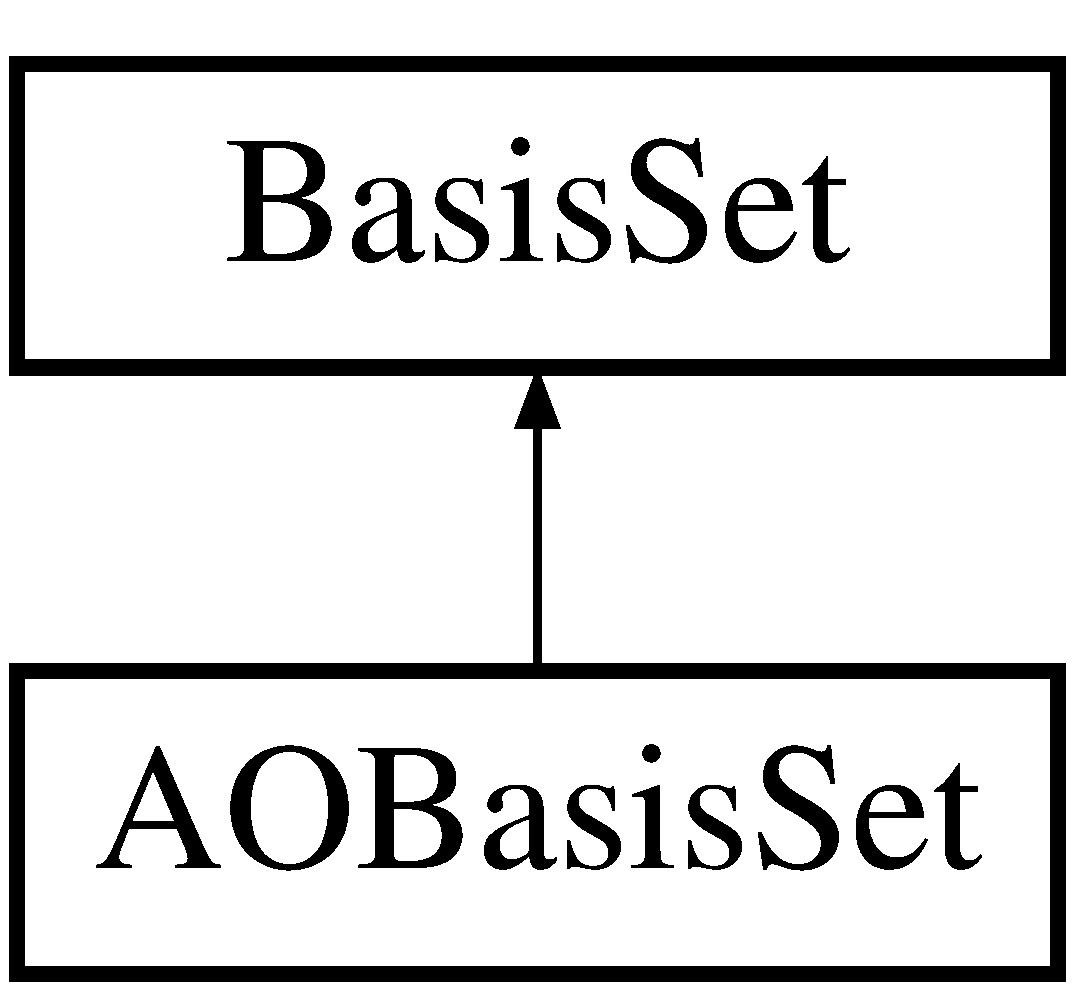
\includegraphics[height=2cm]{classJKBuilder_1_1AOBasisSet}
\end{center}
\end{figure}
\subsection*{Public Member Functions}
\begin{DoxyCompactItemize}
\item 
\hyperlink{classJKBuilder_1_1AOBasisSet_ae37ea5df793e15317b741ddef3065f3a}{AOBasisSet} (\hyperlink{classJKBuilder_1_1molecule__class}{molecule\_\-class} $\ast$molecule)
\begin{DoxyCompactList}\small\item\em Sets up a basis set for the given molecule. \item\end{DoxyCompactList}\item 
\hyperlink{classJKBuilder_1_1AOBasisSet_addb5212a040850c3a3816eb2ef9c2483}{$\sim$AOBasisSet} ()
\begin{DoxyCompactList}\small\item\em Frees memory. \item\end{DoxyCompactList}\item 
int \hyperlink{classJKBuilder_1_1AOBasisSet_aa62be7e63d0f2b5828ab72cec3ce8590}{GetNShells} ()
\begin{DoxyCompactList}\small\item\em Returns the number of shells in the AObasis. \item\end{DoxyCompactList}\item 
int \hyperlink{classJKBuilder_1_1AOBasisSet_a297c144fb990284ac5973c99cdd55f91}{GetNBasis} ()
\begin{DoxyCompactList}\small\item\em Returns the total number of basis functions in the AObasis. \item\end{DoxyCompactList}\item 
int \hyperlink{classJKBuilder_1_1AOBasisSet_af6694a93cc5d86a8f3cd1aa984a0cdc3}{GetMaxL} ()
\begin{DoxyCompactList}\small\item\em Returns the maximum momentum contained in any \hyperlink{classJKBuilder_1_1AtomicBasisSet}{JKBuilder::AtomicBasisSet}. \item\end{DoxyCompactList}\item 
int \hyperlink{classJKBuilder_1_1AOBasisSet_a6a6c8b94fb293123b918605d0507ebbf}{GetNAtoms} ()
\begin{DoxyCompactList}\small\item\em Returns the number of atoms this basis is for. \item\end{DoxyCompactList}\item 
int \hyperlink{classJKBuilder_1_1AOBasisSet_a03191bf41d6e3a2445dd3eb8640305be}{GetMaxPrim} (int \&ID)
\begin{DoxyCompactList}\small\item\em Returns the maximum number of primitives in a shell and sets ID to the ID of that shell. \item\end{DoxyCompactList}\item 
int \hyperlink{classJKBuilder_1_1AOBasisSet_adcda37af511d6b4f8d305fcba2da5c4a}{GetMaxBasis} ()
\begin{DoxyCompactList}\small\item\em Returns the maximum number of basis functions in a shell. \item\end{DoxyCompactList}\item 
\hyperlink{classJKBuilder_1_1AtomicBasisSet}{AtomicBasisSet} $\ast$ \hyperlink{classJKBuilder_1_1AOBasisSet_a1d366290bc84106b0a92c61156a4fa80}{operator\mbox{[}$\,$\mbox{]}} (const int i)
\begin{DoxyCompactList}\small\item\em Returns a pointer to the i-\/th atom's basis set. \item\end{DoxyCompactList}\item 
void \hyperlink{classJKBuilder_1_1AOBasisSet_a388f572c62279f839ee138a9afbdeeb5}{print} ()
\begin{DoxyCompactList}\small\item\em Prints the AO basis set. \item\end{DoxyCompactList}\item 
int \hyperlink{classJKBuilder_1_1AOBasisSet_aa1fc6892f227f640de8bc2d6aa127d5f}{AbsShellNum} (int x, int y)
\begin{DoxyCompactList}\small\item\em Converts shell y, on \hyperlink{classJKBuilder_1_1atom}{atom} x to an absolute number. \item\end{DoxyCompactList}\item 
int \hyperlink{classJKBuilder_1_1AOBasisSet_a23219e59060d6ef915e6146114f52ddd}{AbsBasisNum} (int x, int y, int z)
\begin{DoxyCompactList}\small\item\em Converts basis fxn z, in shell y, on \hyperlink{classJKBuilder_1_1atom}{atom} x to an absolute number by means of AbsShellNum. \item\end{DoxyCompactList}\item 
virtual int \hyperlink{classJKBuilder_1_1BasisSet_abc886cd4e35d3c56a0250b7d06986f61}{GetNPrims} ()
\begin{DoxyCompactList}\small\item\em Returns the number of primitives. \item\end{DoxyCompactList}\end{DoxyCompactItemize}
\subsection*{Protected Attributes}
\begin{DoxyCompactItemize}
\item 
int \hyperlink{classJKBuilder_1_1BasisSet_a41e2bc1e52da2859eabe6586e4451663}{NBasis}
\begin{DoxyCompactList}\small\item\em The number of basis functions in this basis. \item\end{DoxyCompactList}\item 
int \hyperlink{classJKBuilder_1_1BasisSet_a9f13901f058284051a35aabd9d69c6d5}{NShells}
\begin{DoxyCompactList}\small\item\em The number of shells in this basis set. \item\end{DoxyCompactList}\item 
int \hyperlink{classJKBuilder_1_1BasisSet_ad30990632a28f27018d2b497e263caf1}{NPrims}
\begin{DoxyCompactList}\small\item\em The number of primitives in this basis set. \item\end{DoxyCompactList}\item 
int \hyperlink{classJKBuilder_1_1BasisSet_a8fce14d0246c865eea79bf2869b02997}{max\_\-momentum}
\begin{DoxyCompactList}\small\item\em The maximum momentum. \item\end{DoxyCompactList}\item 
int \hyperlink{classJKBuilder_1_1BasisSet_aeb188680b23f4d32ea9a65468e5ba71d}{max\_\-prims}
\begin{DoxyCompactList}\small\item\em The maximum number of primitives. \item\end{DoxyCompactList}\item 
int \hyperlink{classJKBuilder_1_1BasisSet_acdabb925780e7292114dfa2ace8b9d8e}{max\_\-prims\_\-ID}
\begin{DoxyCompactList}\small\item\em The ID of the shell with the maximum number of primitives,counting from 0. \item\end{DoxyCompactList}\item 
int \hyperlink{classJKBuilder_1_1BasisSet_af29e85e56ea63952fc7a1ede8d10426f}{max\_\-basis}
\begin{DoxyCompactList}\small\item\em The maximum number of basis functions in this basis. \item\end{DoxyCompactList}\end{DoxyCompactItemize}
\subsection*{Private Attributes}
\begin{DoxyCompactItemize}
\item 
std::vector$<$ \hyperlink{classJKBuilder_1_1AtomicBasisSet}{AtomicBasisSet} $\ast$ $>$ \hyperlink{classJKBuilder_1_1AOBasisSet_a872dee545656a5acc39da552c8e5137f}{AOBasis}
\begin{DoxyCompactList}\small\item\em The AO basis. \item\end{DoxyCompactList}\item 
std::vector$<$ int $>$ \hyperlink{classJKBuilder_1_1AOBasisSet_a82f86f036166d7d52ed2aea14bfe8510}{ShellsPerAtom}
\item 
std::vector$<$ int $>$ \hyperlink{classJKBuilder_1_1AOBasisSet_a8d80fa437dbb830552ffe2a6b07630fb}{BFsPerShell}
\end{DoxyCompactItemize}


\subsection{Detailed Description}
The top-\/level basis set object for the \hyperlink{namespaceJKBuilder}{JKBuilder} library. ERD and OED integrals are run by shell, so we need details per shell; however each of those shells retains some properties of the atoms they reside on. I have made the decision to store the shells for each \hyperlink{classJKBuilder_1_1atom}{atom} together as objects. The set of all shells for an \hyperlink{classJKBuilder_1_1atom}{atom} is a basis set for that \hyperlink{classJKBuilder_1_1atom}{atom}, an \hyperlink{classJKBuilder_1_1AtomicBasisSet}{JKBuilder::AtomicBasisSet} object. The set of these basis sets for each \hyperlink{classJKBuilder_1_1atom}{atom} in a molecular system is then the \hyperlink{classJKBuilder_1_1AOBasisSet}{AOBasisSet}. That is what is stored in this object. 

\subsection{Constructor \& Destructor Documentation}
\hypertarget{classJKBuilder_1_1AOBasisSet_ae37ea5df793e15317b741ddef3065f3a}{
\index{JKBuilder::AOBasisSet@{JKBuilder::AOBasisSet}!AOBasisSet@{AOBasisSet}}
\index{AOBasisSet@{AOBasisSet}!JKBuilder::AOBasisSet@{JKBuilder::AOBasisSet}}
\subsubsection[{AOBasisSet}]{\setlength{\rightskip}{0pt plus 5cm}{\bf AOBasisSet} ({\bf molecule\_\-class} $\ast$ {\em molecule})}}
\label{classJKBuilder_1_1AOBasisSet_ae37ea5df793e15317b741ddef3065f3a}


Sets up a basis set for the given molecule. 
\begin{DoxyParams}{Parameters}
\item[\mbox{$\leftarrow$} {\em molecule}]The system we are setting up a basis set for \end{DoxyParams}
\hypertarget{classJKBuilder_1_1AOBasisSet_addb5212a040850c3a3816eb2ef9c2483}{
\index{JKBuilder::AOBasisSet@{JKBuilder::AOBasisSet}!$\sim$AOBasisSet@{$\sim$AOBasisSet}}
\index{$\sim$AOBasisSet@{$\sim$AOBasisSet}!JKBuilder::AOBasisSet@{JKBuilder::AOBasisSet}}
\subsubsection[{$\sim$AOBasisSet}]{\setlength{\rightskip}{0pt plus 5cm}$\sim${\bf AOBasisSet} ()}}
\label{classJKBuilder_1_1AOBasisSet_addb5212a040850c3a3816eb2ef9c2483}


Frees memory. 

\subsection{Member Function Documentation}
\hypertarget{classJKBuilder_1_1AOBasisSet_aa62be7e63d0f2b5828ab72cec3ce8590}{
\index{JKBuilder::AOBasisSet@{JKBuilder::AOBasisSet}!GetNShells@{GetNShells}}
\index{GetNShells@{GetNShells}!JKBuilder::AOBasisSet@{JKBuilder::AOBasisSet}}
\subsubsection[{GetNShells}]{\setlength{\rightskip}{0pt plus 5cm}int GetNShells ()\hspace{0.3cm}{\ttfamily  \mbox{[}virtual\mbox{]}}}}
\label{classJKBuilder_1_1AOBasisSet_aa62be7e63d0f2b5828ab72cec3ce8590}


Returns the number of shells in the AObasis. 

Implements \hyperlink{classJKBuilder_1_1BasisSet_a0eb3b46d258dffcfbc3e4db91f60f4f8}{BasisSet}.\hypertarget{classJKBuilder_1_1AOBasisSet_a297c144fb990284ac5973c99cdd55f91}{
\index{JKBuilder::AOBasisSet@{JKBuilder::AOBasisSet}!GetNBasis@{GetNBasis}}
\index{GetNBasis@{GetNBasis}!JKBuilder::AOBasisSet@{JKBuilder::AOBasisSet}}
\subsubsection[{GetNBasis}]{\setlength{\rightskip}{0pt plus 5cm}int GetNBasis ()\hspace{0.3cm}{\ttfamily  \mbox{[}virtual\mbox{]}}}}
\label{classJKBuilder_1_1AOBasisSet_a297c144fb990284ac5973c99cdd55f91}


Returns the total number of basis functions in the AObasis. 

Implements \hyperlink{classJKBuilder_1_1BasisSet_a1167cdb6f1e1ba08ba6cbffa0b32ca77}{BasisSet}.\hypertarget{classJKBuilder_1_1AOBasisSet_af6694a93cc5d86a8f3cd1aa984a0cdc3}{
\index{JKBuilder::AOBasisSet@{JKBuilder::AOBasisSet}!GetMaxL@{GetMaxL}}
\index{GetMaxL@{GetMaxL}!JKBuilder::AOBasisSet@{JKBuilder::AOBasisSet}}
\subsubsection[{GetMaxL}]{\setlength{\rightskip}{0pt plus 5cm}int GetMaxL ()\hspace{0.3cm}{\ttfamily  \mbox{[}virtual\mbox{]}}}}
\label{classJKBuilder_1_1AOBasisSet_af6694a93cc5d86a8f3cd1aa984a0cdc3}


Returns the maximum momentum contained in any \hyperlink{classJKBuilder_1_1AtomicBasisSet}{JKBuilder::AtomicBasisSet}. 

Implements \hyperlink{classJKBuilder_1_1BasisSet_a5580c8eff6cb4242a298c15da2292fa4}{BasisSet}.\hypertarget{classJKBuilder_1_1AOBasisSet_a6a6c8b94fb293123b918605d0507ebbf}{
\index{JKBuilder::AOBasisSet@{JKBuilder::AOBasisSet}!GetNAtoms@{GetNAtoms}}
\index{GetNAtoms@{GetNAtoms}!JKBuilder::AOBasisSet@{JKBuilder::AOBasisSet}}
\subsubsection[{GetNAtoms}]{\setlength{\rightskip}{0pt plus 5cm}int GetNAtoms ()}}
\label{classJKBuilder_1_1AOBasisSet_a6a6c8b94fb293123b918605d0507ebbf}


Returns the number of atoms this basis is for. \hypertarget{classJKBuilder_1_1AOBasisSet_a03191bf41d6e3a2445dd3eb8640305be}{
\index{JKBuilder::AOBasisSet@{JKBuilder::AOBasisSet}!GetMaxPrim@{GetMaxPrim}}
\index{GetMaxPrim@{GetMaxPrim}!JKBuilder::AOBasisSet@{JKBuilder::AOBasisSet}}
\subsubsection[{GetMaxPrim}]{\setlength{\rightskip}{0pt plus 5cm}int GetMaxPrim (int \& {\em ID})\hspace{0.3cm}{\ttfamily  \mbox{[}virtual\mbox{]}}}}
\label{classJKBuilder_1_1AOBasisSet_a03191bf41d6e3a2445dd3eb8640305be}


Returns the maximum number of primitives in a shell and sets ID to the ID of that shell. 

Implements \hyperlink{classJKBuilder_1_1BasisSet_a4e5f8295f4fe1ecf1a910ae2fcb46c1f}{BasisSet}.\hypertarget{classJKBuilder_1_1AOBasisSet_adcda37af511d6b4f8d305fcba2da5c4a}{
\index{JKBuilder::AOBasisSet@{JKBuilder::AOBasisSet}!GetMaxBasis@{GetMaxBasis}}
\index{GetMaxBasis@{GetMaxBasis}!JKBuilder::AOBasisSet@{JKBuilder::AOBasisSet}}
\subsubsection[{GetMaxBasis}]{\setlength{\rightskip}{0pt plus 5cm}int GetMaxBasis ()\hspace{0.3cm}{\ttfamily  \mbox{[}virtual\mbox{]}}}}
\label{classJKBuilder_1_1AOBasisSet_adcda37af511d6b4f8d305fcba2da5c4a}


Returns the maximum number of basis functions in a shell. 

Implements \hyperlink{classJKBuilder_1_1BasisSet_a7c12871050e478f6a22c4c1c46bd4b21}{BasisSet}.\hypertarget{classJKBuilder_1_1AOBasisSet_a1d366290bc84106b0a92c61156a4fa80}{
\index{JKBuilder::AOBasisSet@{JKBuilder::AOBasisSet}!operator\mbox{[}\mbox{]}@{operator[]}}
\index{operator\mbox{[}\mbox{]}@{operator[]}!JKBuilder::AOBasisSet@{JKBuilder::AOBasisSet}}
\subsubsection[{operator[]}]{\setlength{\rightskip}{0pt plus 5cm}{\bf AtomicBasisSet} $\ast$ operator\mbox{[}$\,$\mbox{]} (const int {\em i})}}
\label{classJKBuilder_1_1AOBasisSet_a1d366290bc84106b0a92c61156a4fa80}


Returns a pointer to the i-\/th atom's basis set. \hypertarget{classJKBuilder_1_1AOBasisSet_a388f572c62279f839ee138a9afbdeeb5}{
\index{JKBuilder::AOBasisSet@{JKBuilder::AOBasisSet}!print@{print}}
\index{print@{print}!JKBuilder::AOBasisSet@{JKBuilder::AOBasisSet}}
\subsubsection[{print}]{\setlength{\rightskip}{0pt plus 5cm}void print ()\hspace{0.3cm}{\ttfamily  \mbox{[}virtual\mbox{]}}}}
\label{classJKBuilder_1_1AOBasisSet_a388f572c62279f839ee138a9afbdeeb5}


Prints the AO basis set. 

Reimplemented from \hyperlink{classJKBuilder_1_1BasisSet_a388f572c62279f839ee138a9afbdeeb5}{BasisSet}.\hypertarget{classJKBuilder_1_1AOBasisSet_aa1fc6892f227f640de8bc2d6aa127d5f}{
\index{JKBuilder::AOBasisSet@{JKBuilder::AOBasisSet}!AbsShellNum@{AbsShellNum}}
\index{AbsShellNum@{AbsShellNum}!JKBuilder::AOBasisSet@{JKBuilder::AOBasisSet}}
\subsubsection[{AbsShellNum}]{\setlength{\rightskip}{0pt plus 5cm}int AbsShellNum (int {\em x}, \/  int {\em y})}}
\label{classJKBuilder_1_1AOBasisSet_aa1fc6892f227f640de8bc2d6aa127d5f}


Converts shell y, on \hyperlink{classJKBuilder_1_1atom}{atom} x to an absolute number. \hypertarget{classJKBuilder_1_1AOBasisSet_a23219e59060d6ef915e6146114f52ddd}{
\index{JKBuilder::AOBasisSet@{JKBuilder::AOBasisSet}!AbsBasisNum@{AbsBasisNum}}
\index{AbsBasisNum@{AbsBasisNum}!JKBuilder::AOBasisSet@{JKBuilder::AOBasisSet}}
\subsubsection[{AbsBasisNum}]{\setlength{\rightskip}{0pt plus 5cm}int AbsBasisNum (int {\em x}, \/  int {\em y}, \/  int {\em z})}}
\label{classJKBuilder_1_1AOBasisSet_a23219e59060d6ef915e6146114f52ddd}


Converts basis fxn z, in shell y, on \hyperlink{classJKBuilder_1_1atom}{atom} x to an absolute number by means of AbsShellNum. \hypertarget{classJKBuilder_1_1BasisSet_abc886cd4e35d3c56a0250b7d06986f61}{
\index{JKBuilder::AOBasisSet@{JKBuilder::AOBasisSet}!GetNPrims@{GetNPrims}}
\index{GetNPrims@{GetNPrims}!JKBuilder::AOBasisSet@{JKBuilder::AOBasisSet}}
\subsubsection[{GetNPrims}]{\setlength{\rightskip}{0pt plus 5cm}int GetNPrims ()\hspace{0.3cm}{\ttfamily  \mbox{[}virtual, inherited\mbox{]}}}}
\label{classJKBuilder_1_1BasisSet_abc886cd4e35d3c56a0250b7d06986f61}


Returns the number of primitives. 

\subsection{Member Data Documentation}
\hypertarget{classJKBuilder_1_1AOBasisSet_a872dee545656a5acc39da552c8e5137f}{
\index{JKBuilder::AOBasisSet@{JKBuilder::AOBasisSet}!AOBasis@{AOBasis}}
\index{AOBasis@{AOBasis}!JKBuilder::AOBasisSet@{JKBuilder::AOBasisSet}}
\subsubsection[{AOBasis}]{\setlength{\rightskip}{0pt plus 5cm}std::vector$<${\bf AtomicBasisSet}$\ast$$>$ {\bf AOBasis}\hspace{0.3cm}{\ttfamily  \mbox{[}private\mbox{]}}}}
\label{classJKBuilder_1_1AOBasisSet_a872dee545656a5acc39da552c8e5137f}


The AO basis. A vector of the basis sets for each \hyperlink{classJKBuilder_1_1atom}{atom}, this is the AO basis. The order of the AtomicBasisSets that are on it is expected to correspond to the order the atoms are in the input file. That is AOBasis\mbox{[}i\mbox{]} should be the basis set of \hyperlink{classJKBuilder_1_1atom}{atom} i,counting from 0. \hypertarget{classJKBuilder_1_1AOBasisSet_a82f86f036166d7d52ed2aea14bfe8510}{
\index{JKBuilder::AOBasisSet@{JKBuilder::AOBasisSet}!ShellsPerAtom@{ShellsPerAtom}}
\index{ShellsPerAtom@{ShellsPerAtom}!JKBuilder::AOBasisSet@{JKBuilder::AOBasisSet}}
\subsubsection[{ShellsPerAtom}]{\setlength{\rightskip}{0pt plus 5cm}std::vector$<$int$>$ {\bf ShellsPerAtom}\hspace{0.3cm}{\ttfamily  \mbox{[}private\mbox{]}}}}
\label{classJKBuilder_1_1AOBasisSet_a82f86f036166d7d52ed2aea14bfe8510}
\hypertarget{classJKBuilder_1_1AOBasisSet_a8d80fa437dbb830552ffe2a6b07630fb}{
\index{JKBuilder::AOBasisSet@{JKBuilder::AOBasisSet}!BFsPerShell@{BFsPerShell}}
\index{BFsPerShell@{BFsPerShell}!JKBuilder::AOBasisSet@{JKBuilder::AOBasisSet}}
\subsubsection[{BFsPerShell}]{\setlength{\rightskip}{0pt plus 5cm}std::vector$<$int$>$ {\bf BFsPerShell}\hspace{0.3cm}{\ttfamily  \mbox{[}private\mbox{]}}}}
\label{classJKBuilder_1_1AOBasisSet_a8d80fa437dbb830552ffe2a6b07630fb}
\hypertarget{classJKBuilder_1_1BasisSet_a41e2bc1e52da2859eabe6586e4451663}{
\index{JKBuilder::AOBasisSet@{JKBuilder::AOBasisSet}!NBasis@{NBasis}}
\index{NBasis@{NBasis}!JKBuilder::AOBasisSet@{JKBuilder::AOBasisSet}}
\subsubsection[{NBasis}]{\setlength{\rightskip}{0pt plus 5cm}int {\bf NBasis}\hspace{0.3cm}{\ttfamily  \mbox{[}protected, inherited\mbox{]}}}}
\label{classJKBuilder_1_1BasisSet_a41e2bc1e52da2859eabe6586e4451663}


The number of basis functions in this basis. \hypertarget{classJKBuilder_1_1BasisSet_a9f13901f058284051a35aabd9d69c6d5}{
\index{JKBuilder::AOBasisSet@{JKBuilder::AOBasisSet}!NShells@{NShells}}
\index{NShells@{NShells}!JKBuilder::AOBasisSet@{JKBuilder::AOBasisSet}}
\subsubsection[{NShells}]{\setlength{\rightskip}{0pt plus 5cm}int {\bf NShells}\hspace{0.3cm}{\ttfamily  \mbox{[}protected, inherited\mbox{]}}}}
\label{classJKBuilder_1_1BasisSet_a9f13901f058284051a35aabd9d69c6d5}


The number of shells in this basis set. \hypertarget{classJKBuilder_1_1BasisSet_ad30990632a28f27018d2b497e263caf1}{
\index{JKBuilder::AOBasisSet@{JKBuilder::AOBasisSet}!NPrims@{NPrims}}
\index{NPrims@{NPrims}!JKBuilder::AOBasisSet@{JKBuilder::AOBasisSet}}
\subsubsection[{NPrims}]{\setlength{\rightskip}{0pt plus 5cm}int {\bf NPrims}\hspace{0.3cm}{\ttfamily  \mbox{[}protected, inherited\mbox{]}}}}
\label{classJKBuilder_1_1BasisSet_ad30990632a28f27018d2b497e263caf1}


The number of primitives in this basis set. \hypertarget{classJKBuilder_1_1BasisSet_a8fce14d0246c865eea79bf2869b02997}{
\index{JKBuilder::AOBasisSet@{JKBuilder::AOBasisSet}!max\_\-momentum@{max\_\-momentum}}
\index{max\_\-momentum@{max\_\-momentum}!JKBuilder::AOBasisSet@{JKBuilder::AOBasisSet}}
\subsubsection[{max\_\-momentum}]{\setlength{\rightskip}{0pt plus 5cm}int {\bf max\_\-momentum}\hspace{0.3cm}{\ttfamily  \mbox{[}protected, inherited\mbox{]}}}}
\label{classJKBuilder_1_1BasisSet_a8fce14d0246c865eea79bf2869b02997}


The maximum momentum. \hypertarget{classJKBuilder_1_1BasisSet_aeb188680b23f4d32ea9a65468e5ba71d}{
\index{JKBuilder::AOBasisSet@{JKBuilder::AOBasisSet}!max\_\-prims@{max\_\-prims}}
\index{max\_\-prims@{max\_\-prims}!JKBuilder::AOBasisSet@{JKBuilder::AOBasisSet}}
\subsubsection[{max\_\-prims}]{\setlength{\rightskip}{0pt plus 5cm}int {\bf max\_\-prims}\hspace{0.3cm}{\ttfamily  \mbox{[}protected, inherited\mbox{]}}}}
\label{classJKBuilder_1_1BasisSet_aeb188680b23f4d32ea9a65468e5ba71d}


The maximum number of primitives. \hypertarget{classJKBuilder_1_1BasisSet_acdabb925780e7292114dfa2ace8b9d8e}{
\index{JKBuilder::AOBasisSet@{JKBuilder::AOBasisSet}!max\_\-prims\_\-ID@{max\_\-prims\_\-ID}}
\index{max\_\-prims\_\-ID@{max\_\-prims\_\-ID}!JKBuilder::AOBasisSet@{JKBuilder::AOBasisSet}}
\subsubsection[{max\_\-prims\_\-ID}]{\setlength{\rightskip}{0pt plus 5cm}int {\bf max\_\-prims\_\-ID}\hspace{0.3cm}{\ttfamily  \mbox{[}protected, inherited\mbox{]}}}}
\label{classJKBuilder_1_1BasisSet_acdabb925780e7292114dfa2ace8b9d8e}


The ID of the shell with the maximum number of primitives,counting from 0. \hypertarget{classJKBuilder_1_1BasisSet_af29e85e56ea63952fc7a1ede8d10426f}{
\index{JKBuilder::AOBasisSet@{JKBuilder::AOBasisSet}!max\_\-basis@{max\_\-basis}}
\index{max\_\-basis@{max\_\-basis}!JKBuilder::AOBasisSet@{JKBuilder::AOBasisSet}}
\subsubsection[{max\_\-basis}]{\setlength{\rightskip}{0pt plus 5cm}int {\bf max\_\-basis}\hspace{0.3cm}{\ttfamily  \mbox{[}protected, inherited\mbox{]}}}}
\label{classJKBuilder_1_1BasisSet_af29e85e56ea63952fc7a1ede8d10426f}


The maximum number of basis functions in this basis. 

The documentation for this class was generated from the following files:\begin{DoxyCompactItemize}
\item 
src/\hyperlink{BasisSet_8h}{BasisSet.h}\item 
src/\hyperlink{BasisSet_8cpp}{BasisSet.cpp}\end{DoxyCompactItemize}

\hypertarget{classJKBuilder_1_1atom}{
\section{atom Class Reference}
\label{classJKBuilder_1_1atom}\index{JKBuilder::atom@{JKBuilder::atom}}
}


{\ttfamily \#include $<$molecule.h$>$}\subsection*{Public Member Functions}
\begin{DoxyCompactItemize}
\item 
\hyperlink{classJKBuilder_1_1atom_a093b616ad3671037f440a6fa34ab6355}{atom} (const int Z\_\-, const double $\ast$carts\_\-, bool bohr=false)
\begin{DoxyCompactList}\small\item\em Creates an \hyperlink{classJKBuilder_1_1atom}{atom}. \item\end{DoxyCompactList}\item 
const double \& \hyperlink{classJKBuilder_1_1atom_a4f0dc1b84b580cec49500c70f87e084a}{operator\mbox{[}$\,$\mbox{]}} (const int i) const 
\begin{DoxyCompactList}\small\item\em Returns the i-\/th coordinate of the \hyperlink{classJKBuilder_1_1atom}{atom} (x=0,y=1,z=2). \item\end{DoxyCompactList}\item 
int \hyperlink{classJKBuilder_1_1atom_a57becd9a69927a5ba8ae251a7790dc2a}{GetZ} () const 
\begin{DoxyCompactList}\small\item\em Returns the atomic number. \item\end{DoxyCompactList}\item 
std::string \hyperlink{classJKBuilder_1_1atom_a41d45f22912b0c077a76b7a4234599b6}{print} () const 
\begin{DoxyCompactList}\small\item\em returns the chemical symbol and carts suitable for printing \item\end{DoxyCompactList}\item 
int \hyperlink{classJKBuilder_1_1atom_aeb29d9144c99d302f7b43d5398929ea5}{GetNelec} () const 
\begin{DoxyCompactList}\small\item\em Returns the number of electrons (calls GetZ). \item\end{DoxyCompactList}\end{DoxyCompactItemize}
\subsection*{Private Member Functions}
\begin{DoxyCompactItemize}
\item 
std::string \hyperlink{classJKBuilder_1_1atom_a163d1d4c84461da513e1d1346cb1b407}{ZtoAt} (const int \hyperlink{classJKBuilder_1_1atom_a5ed5bfe6933ed8cba853237650cc041b}{Z}) const 
\begin{DoxyCompactList}\small\item\em Function that returns the chemical symbol of atomic number Z in all uppercase letters. \item\end{DoxyCompactList}\end{DoxyCompactItemize}
\subsection*{Private Attributes}
\begin{DoxyCompactItemize}
\item 
int \hyperlink{classJKBuilder_1_1atom_a5ed5bfe6933ed8cba853237650cc041b}{Z}
\begin{DoxyCompactList}\small\item\em Atomic number (between 1 and 36 for now). \item\end{DoxyCompactList}\item 
int \hyperlink{classJKBuilder_1_1atom_a849e4a1d5fee0c024e42b658d3babd02}{Nelec}
\begin{DoxyCompactList}\small\item\em The number of electrons. \item\end{DoxyCompactList}\item 
double \hyperlink{classJKBuilder_1_1atom_a6b5adb6f3635311b52c7a7a35dcb01b4}{carts} \mbox{[}3\mbox{]}
\begin{DoxyCompactList}\small\item\em Carts in bohr. \item\end{DoxyCompactList}\end{DoxyCompactItemize}


\subsection{Constructor \& Destructor Documentation}
\hypertarget{classJKBuilder_1_1atom_a093b616ad3671037f440a6fa34ab6355}{
\index{JKBuilder::atom@{JKBuilder::atom}!atom@{atom}}
\index{atom@{atom}!JKBuilder::atom@{JKBuilder::atom}}
\subsubsection[{atom}]{\setlength{\rightskip}{0pt plus 5cm}{\bf atom} (const int {\em Z\_\-}, \/  const double $\ast$ {\em carts\_\-}, \/  bool {\em bohr} = {\ttfamily false})}}
\label{classJKBuilder_1_1atom_a093b616ad3671037f440a6fa34ab6355}


Creates an \hyperlink{classJKBuilder_1_1atom}{atom}. 
\begin{DoxyParams}{Parameters}
\item[\mbox{$\leftarrow$} {\em Z\_\-}]is the atomic number \item[\mbox{$\leftarrow$} {\em carts\_\-}]is a 3 element array where carts\_\-\mbox{[}0\mbox{]},carts\mbox{[}1\mbox{]}, and carts\mbox{[}2\mbox{]} are the x,y, and z coordinates of the \hyperlink{classJKBuilder_1_1atom}{atom} \item[\mbox{$\leftarrow$} {\em bohr}]True means the carts that are passed in are in atomic units, false means they are in Angstroms, default is false \end{DoxyParams}


\subsection{Member Function Documentation}
\hypertarget{classJKBuilder_1_1atom_a163d1d4c84461da513e1d1346cb1b407}{
\index{JKBuilder::atom@{JKBuilder::atom}!ZtoAt@{ZtoAt}}
\index{ZtoAt@{ZtoAt}!JKBuilder::atom@{JKBuilder::atom}}
\subsubsection[{ZtoAt}]{\setlength{\rightskip}{0pt plus 5cm}string ZtoAt (const int {\em Z}) const\hspace{0.3cm}{\ttfamily  \mbox{[}private\mbox{]}}}}
\label{classJKBuilder_1_1atom_a163d1d4c84461da513e1d1346cb1b407}


Function that returns the chemical symbol of atomic number Z in all uppercase letters. \hypertarget{classJKBuilder_1_1atom_a4f0dc1b84b580cec49500c70f87e084a}{
\index{JKBuilder::atom@{JKBuilder::atom}!operator\mbox{[}\mbox{]}@{operator[]}}
\index{operator\mbox{[}\mbox{]}@{operator[]}!JKBuilder::atom@{JKBuilder::atom}}
\subsubsection[{operator[]}]{\setlength{\rightskip}{0pt plus 5cm}const double \& operator\mbox{[}$\,$\mbox{]} (const int {\em i}) const}}
\label{classJKBuilder_1_1atom_a4f0dc1b84b580cec49500c70f87e084a}


Returns the i-\/th coordinate of the \hyperlink{classJKBuilder_1_1atom}{atom} (x=0,y=1,z=2). \hypertarget{classJKBuilder_1_1atom_a57becd9a69927a5ba8ae251a7790dc2a}{
\index{JKBuilder::atom@{JKBuilder::atom}!GetZ@{GetZ}}
\index{GetZ@{GetZ}!JKBuilder::atom@{JKBuilder::atom}}
\subsubsection[{GetZ}]{\setlength{\rightskip}{0pt plus 5cm}int GetZ () const}}
\label{classJKBuilder_1_1atom_a57becd9a69927a5ba8ae251a7790dc2a}


Returns the atomic number. \hypertarget{classJKBuilder_1_1atom_a41d45f22912b0c077a76b7a4234599b6}{
\index{JKBuilder::atom@{JKBuilder::atom}!print@{print}}
\index{print@{print}!JKBuilder::atom@{JKBuilder::atom}}
\subsubsection[{print}]{\setlength{\rightskip}{0pt plus 5cm}string print () const}}
\label{classJKBuilder_1_1atom_a41d45f22912b0c077a76b7a4234599b6}


returns the chemical symbol and carts suitable for printing \hypertarget{classJKBuilder_1_1atom_aeb29d9144c99d302f7b43d5398929ea5}{
\index{JKBuilder::atom@{JKBuilder::atom}!GetNelec@{GetNelec}}
\index{GetNelec@{GetNelec}!JKBuilder::atom@{JKBuilder::atom}}
\subsubsection[{GetNelec}]{\setlength{\rightskip}{0pt plus 5cm}int GetNelec () const}}
\label{classJKBuilder_1_1atom_aeb29d9144c99d302f7b43d5398929ea5}


Returns the number of electrons (calls GetZ). 

\subsection{Member Data Documentation}
\hypertarget{classJKBuilder_1_1atom_a5ed5bfe6933ed8cba853237650cc041b}{
\index{JKBuilder::atom@{JKBuilder::atom}!Z@{Z}}
\index{Z@{Z}!JKBuilder::atom@{JKBuilder::atom}}
\subsubsection[{Z}]{\setlength{\rightskip}{0pt plus 5cm}int {\bf Z}\hspace{0.3cm}{\ttfamily  \mbox{[}private\mbox{]}}}}
\label{classJKBuilder_1_1atom_a5ed5bfe6933ed8cba853237650cc041b}


Atomic number (between 1 and 36 for now). \hypertarget{classJKBuilder_1_1atom_a849e4a1d5fee0c024e42b658d3babd02}{
\index{JKBuilder::atom@{JKBuilder::atom}!Nelec@{Nelec}}
\index{Nelec@{Nelec}!JKBuilder::atom@{JKBuilder::atom}}
\subsubsection[{Nelec}]{\setlength{\rightskip}{0pt plus 5cm}int {\bf Nelec}\hspace{0.3cm}{\ttfamily  \mbox{[}private\mbox{]}}}}
\label{classJKBuilder_1_1atom_a849e4a1d5fee0c024e42b658d3babd02}


The number of electrons. \hypertarget{classJKBuilder_1_1atom_a6b5adb6f3635311b52c7a7a35dcb01b4}{
\index{JKBuilder::atom@{JKBuilder::atom}!carts@{carts}}
\index{carts@{carts}!JKBuilder::atom@{JKBuilder::atom}}
\subsubsection[{carts}]{\setlength{\rightskip}{0pt plus 5cm}double {\bf carts}\mbox{[}3\mbox{]}\hspace{0.3cm}{\ttfamily  \mbox{[}private\mbox{]}}}}
\label{classJKBuilder_1_1atom_a6b5adb6f3635311b52c7a7a35dcb01b4}


Carts in bohr. 

The documentation for this class was generated from the following files:\begin{DoxyCompactItemize}
\item 
src/\hyperlink{molecule_8h}{molecule.h}\item 
src/\hyperlink{molecule_8cpp}{molecule.cpp}\end{DoxyCompactItemize}

\hypertarget{classJKBuilder_1_1AtomicBasisSet}{
\section{AtomicBasisSet Class Reference}
\label{classJKBuilder_1_1AtomicBasisSet}\index{JKBuilder::AtomicBasisSet@{JKBuilder::AtomicBasisSet}}
}


{\ttfamily \#include $<$BasisSet.h$>$}Inheritance diagram for AtomicBasisSet::\begin{figure}[H]
\begin{center}
\leavevmode
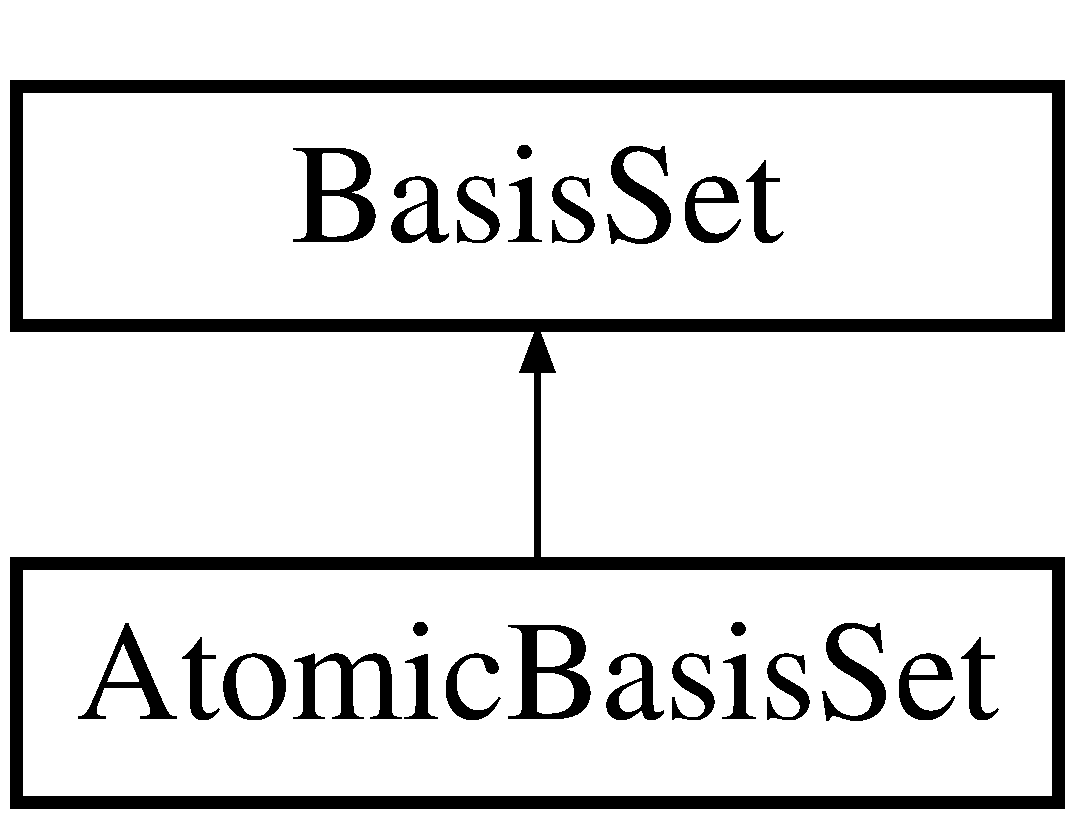
\includegraphics[height=2cm]{classJKBuilder_1_1AtomicBasisSet}
\end{center}
\end{figure}
\subsection*{Public Member Functions}
\begin{DoxyCompactItemize}
\item 
\hyperlink{classJKBuilder_1_1AtomicBasisSet_aba418bbf95a1242f52a30da3bfd01b8c}{AtomicBasisSet} (const double $\ast$Carts)
\begin{DoxyCompactList}\small\item\em Creates a basis set for an \hyperlink{classJKBuilder_1_1atom}{atom}. \item\end{DoxyCompactList}\item 
\hyperlink{classJKBuilder_1_1AtomicBasisSet_a7c7450d3b14d5416225a628fbdff0a1a}{$\sim$AtomicBasisSet} ()
\begin{DoxyCompactList}\small\item\em Frees the memory associated with the shells. \item\end{DoxyCompactList}\item 
void \hyperlink{classJKBuilder_1_1AtomicBasisSet_aad8da23b7ac00a4855a0eed27e9af7cd}{AddShell} (int l, bool isCart)
\begin{DoxyCompactList}\small\item\em Creates a new shell. \item\end{DoxyCompactList}\item 
int \hyperlink{classJKBuilder_1_1AtomicBasisSet_aa62be7e63d0f2b5828ab72cec3ce8590}{GetNShells} ()
\begin{DoxyCompactList}\small\item\em Returns the number of shells. \item\end{DoxyCompactList}\item 
int \hyperlink{classJKBuilder_1_1AtomicBasisSet_a297c144fb990284ac5973c99cdd55f91}{GetNBasis} ()
\begin{DoxyCompactList}\small\item\em Returns the number of basis functions. \item\end{DoxyCompactList}\item 
int \hyperlink{classJKBuilder_1_1AtomicBasisSet_af6694a93cc5d86a8f3cd1aa984a0cdc3}{GetMaxL} ()
\begin{DoxyCompactList}\small\item\em Returns the maximum angular momentum. \item\end{DoxyCompactList}\item 
int \hyperlink{classJKBuilder_1_1AtomicBasisSet_a03191bf41d6e3a2445dd3eb8640305be}{GetMaxPrim} (int \&ID)
\begin{DoxyCompactList}\small\item\em Returns the maximum number of primitives. \item\end{DoxyCompactList}\item 
int \hyperlink{classJKBuilder_1_1AtomicBasisSet_adcda37af511d6b4f8d305fcba2da5c4a}{GetMaxBasis} ()
\begin{DoxyCompactList}\small\item\em Returns the maximum number of basis functions in a shell. \item\end{DoxyCompactList}\item 
\hyperlink{classJKBuilder_1_1Shell}{Shell} $\ast$ \hyperlink{classJKBuilder_1_1AtomicBasisSet_a6da2f2341be7b61c7221afb16fdd72db}{operator\mbox{[}$\,$\mbox{]}} (const int i)
\begin{DoxyCompactList}\small\item\em Returns the i-\/th shell of this basis set. \item\end{DoxyCompactList}\item 
void \hyperlink{classJKBuilder_1_1AtomicBasisSet_a388f572c62279f839ee138a9afbdeeb5}{print} ()
\begin{DoxyCompactList}\small\item\em Prints the basis set. \item\end{DoxyCompactList}\item 
virtual int \hyperlink{classJKBuilder_1_1BasisSet_abc886cd4e35d3c56a0250b7d06986f61}{GetNPrims} ()
\begin{DoxyCompactList}\small\item\em Returns the number of primitives. \item\end{DoxyCompactList}\end{DoxyCompactItemize}
\subsection*{Protected Attributes}
\begin{DoxyCompactItemize}
\item 
int \hyperlink{classJKBuilder_1_1BasisSet_a41e2bc1e52da2859eabe6586e4451663}{NBasis}
\begin{DoxyCompactList}\small\item\em The number of basis functions in this basis. \item\end{DoxyCompactList}\item 
int \hyperlink{classJKBuilder_1_1BasisSet_a9f13901f058284051a35aabd9d69c6d5}{NShells}
\begin{DoxyCompactList}\small\item\em The number of shells in this basis set. \item\end{DoxyCompactList}\item 
int \hyperlink{classJKBuilder_1_1BasisSet_ad30990632a28f27018d2b497e263caf1}{NPrims}
\begin{DoxyCompactList}\small\item\em The number of primitives in this basis set. \item\end{DoxyCompactList}\item 
int \hyperlink{classJKBuilder_1_1BasisSet_a8fce14d0246c865eea79bf2869b02997}{max\_\-momentum}
\begin{DoxyCompactList}\small\item\em The maximum momentum. \item\end{DoxyCompactList}\item 
int \hyperlink{classJKBuilder_1_1BasisSet_aeb188680b23f4d32ea9a65468e5ba71d}{max\_\-prims}
\begin{DoxyCompactList}\small\item\em The maximum number of primitives. \item\end{DoxyCompactList}\item 
int \hyperlink{classJKBuilder_1_1BasisSet_acdabb925780e7292114dfa2ace8b9d8e}{max\_\-prims\_\-ID}
\begin{DoxyCompactList}\small\item\em The ID of the shell with the maximum number of primitives,counting from 0. \item\end{DoxyCompactList}\item 
int \hyperlink{classJKBuilder_1_1BasisSet_af29e85e56ea63952fc7a1ede8d10426f}{max\_\-basis}
\begin{DoxyCompactList}\small\item\em The maximum number of basis functions in this basis. \item\end{DoxyCompactList}\end{DoxyCompactItemize}
\subsection*{Private Attributes}
\begin{DoxyCompactItemize}
\item 
double \hyperlink{classJKBuilder_1_1AtomicBasisSet_a6b5adb6f3635311b52c7a7a35dcb01b4}{carts} \mbox{[}3\mbox{]}
\begin{DoxyCompactList}\small\item\em The coordinates (bohr) of this \hyperlink{classJKBuilder_1_1atom}{atom}, and therefore the coordinates of the center of each of its shells. \item\end{DoxyCompactList}\item 
std::vector$<$ \hyperlink{classJKBuilder_1_1Shell}{Shell} $\ast$ $>$ \hyperlink{classJKBuilder_1_1AtomicBasisSet_a26a4de72845629b10ccfa84bf3b27790}{shells}
\begin{DoxyCompactList}\small\item\em The shells of this atom's basis set. \item\end{DoxyCompactList}\end{DoxyCompactItemize}


\subsection{Constructor \& Destructor Documentation}
\hypertarget{classJKBuilder_1_1AtomicBasisSet_aba418bbf95a1242f52a30da3bfd01b8c}{
\index{JKBuilder::AtomicBasisSet@{JKBuilder::AtomicBasisSet}!AtomicBasisSet@{AtomicBasisSet}}
\index{AtomicBasisSet@{AtomicBasisSet}!JKBuilder::AtomicBasisSet@{JKBuilder::AtomicBasisSet}}
\subsubsection[{AtomicBasisSet}]{\setlength{\rightskip}{0pt plus 5cm}{\bf AtomicBasisSet} (const double $\ast$ {\em Carts})}}
\label{classJKBuilder_1_1AtomicBasisSet_aba418bbf95a1242f52a30da3bfd01b8c}


Creates a basis set for an \hyperlink{classJKBuilder_1_1atom}{atom}. 
\begin{DoxyParams}{Parameters}
\item[\mbox{$\leftarrow$} {\em Carts}]The coordinates of the point in space upon which this shell is centered \end{DoxyParams}
\hypertarget{classJKBuilder_1_1AtomicBasisSet_a7c7450d3b14d5416225a628fbdff0a1a}{
\index{JKBuilder::AtomicBasisSet@{JKBuilder::AtomicBasisSet}!$\sim$AtomicBasisSet@{$\sim$AtomicBasisSet}}
\index{$\sim$AtomicBasisSet@{$\sim$AtomicBasisSet}!JKBuilder::AtomicBasisSet@{JKBuilder::AtomicBasisSet}}
\subsubsection[{$\sim$AtomicBasisSet}]{\setlength{\rightskip}{0pt plus 5cm}$\sim${\bf AtomicBasisSet} ()}}
\label{classJKBuilder_1_1AtomicBasisSet_a7c7450d3b14d5416225a628fbdff0a1a}


Frees the memory associated with the shells. 

\subsection{Member Function Documentation}
\hypertarget{classJKBuilder_1_1AtomicBasisSet_aad8da23b7ac00a4855a0eed27e9af7cd}{
\index{JKBuilder::AtomicBasisSet@{JKBuilder::AtomicBasisSet}!AddShell@{AddShell}}
\index{AddShell@{AddShell}!JKBuilder::AtomicBasisSet@{JKBuilder::AtomicBasisSet}}
\subsubsection[{AddShell}]{\setlength{\rightskip}{0pt plus 5cm}void AddShell (int {\em l}, \/  bool {\em isCart})}}
\label{classJKBuilder_1_1AtomicBasisSet_aad8da23b7ac00a4855a0eed27e9af7cd}


Creates a new shell. This function creates new shells. It also keeps track of the angular momentum and the number of shells 
\begin{DoxyParams}{Parameters}
\item[\mbox{$\leftarrow$} {\em l}]The angular momentum of the shell \item[\mbox{$\leftarrow$} {\em isCart}]True if the orbitals in this shell are Cartesian-\/like, for spherical-\/like use false \end{DoxyParams}
\hypertarget{classJKBuilder_1_1AtomicBasisSet_aa62be7e63d0f2b5828ab72cec3ce8590}{
\index{JKBuilder::AtomicBasisSet@{JKBuilder::AtomicBasisSet}!GetNShells@{GetNShells}}
\index{GetNShells@{GetNShells}!JKBuilder::AtomicBasisSet@{JKBuilder::AtomicBasisSet}}
\subsubsection[{GetNShells}]{\setlength{\rightskip}{0pt plus 5cm}int GetNShells ()\hspace{0.3cm}{\ttfamily  \mbox{[}virtual\mbox{]}}}}
\label{classJKBuilder_1_1AtomicBasisSet_aa62be7e63d0f2b5828ab72cec3ce8590}


Returns the number of shells. 

Implements \hyperlink{classJKBuilder_1_1BasisSet_a0eb3b46d258dffcfbc3e4db91f60f4f8}{BasisSet}.\hypertarget{classJKBuilder_1_1AtomicBasisSet_a297c144fb990284ac5973c99cdd55f91}{
\index{JKBuilder::AtomicBasisSet@{JKBuilder::AtomicBasisSet}!GetNBasis@{GetNBasis}}
\index{GetNBasis@{GetNBasis}!JKBuilder::AtomicBasisSet@{JKBuilder::AtomicBasisSet}}
\subsubsection[{GetNBasis}]{\setlength{\rightskip}{0pt plus 5cm}int GetNBasis ()\hspace{0.3cm}{\ttfamily  \mbox{[}virtual\mbox{]}}}}
\label{classJKBuilder_1_1AtomicBasisSet_a297c144fb990284ac5973c99cdd55f91}


Returns the number of basis functions. 

Implements \hyperlink{classJKBuilder_1_1BasisSet_a1167cdb6f1e1ba08ba6cbffa0b32ca77}{BasisSet}.\hypertarget{classJKBuilder_1_1AtomicBasisSet_af6694a93cc5d86a8f3cd1aa984a0cdc3}{
\index{JKBuilder::AtomicBasisSet@{JKBuilder::AtomicBasisSet}!GetMaxL@{GetMaxL}}
\index{GetMaxL@{GetMaxL}!JKBuilder::AtomicBasisSet@{JKBuilder::AtomicBasisSet}}
\subsubsection[{GetMaxL}]{\setlength{\rightskip}{0pt plus 5cm}int GetMaxL ()\hspace{0.3cm}{\ttfamily  \mbox{[}virtual\mbox{]}}}}
\label{classJKBuilder_1_1AtomicBasisSet_af6694a93cc5d86a8f3cd1aa984a0cdc3}


Returns the maximum angular momentum. 

Implements \hyperlink{classJKBuilder_1_1BasisSet_a5580c8eff6cb4242a298c15da2292fa4}{BasisSet}.\hypertarget{classJKBuilder_1_1AtomicBasisSet_a03191bf41d6e3a2445dd3eb8640305be}{
\index{JKBuilder::AtomicBasisSet@{JKBuilder::AtomicBasisSet}!GetMaxPrim@{GetMaxPrim}}
\index{GetMaxPrim@{GetMaxPrim}!JKBuilder::AtomicBasisSet@{JKBuilder::AtomicBasisSet}}
\subsubsection[{GetMaxPrim}]{\setlength{\rightskip}{0pt plus 5cm}int GetMaxPrim (int \& {\em ID})\hspace{0.3cm}{\ttfamily  \mbox{[}virtual\mbox{]}}}}
\label{classJKBuilder_1_1AtomicBasisSet_a03191bf41d6e3a2445dd3eb8640305be}


Returns the maximum number of primitives. 

Implements \hyperlink{classJKBuilder_1_1BasisSet_a4e5f8295f4fe1ecf1a910ae2fcb46c1f}{BasisSet}.\hypertarget{classJKBuilder_1_1AtomicBasisSet_adcda37af511d6b4f8d305fcba2da5c4a}{
\index{JKBuilder::AtomicBasisSet@{JKBuilder::AtomicBasisSet}!GetMaxBasis@{GetMaxBasis}}
\index{GetMaxBasis@{GetMaxBasis}!JKBuilder::AtomicBasisSet@{JKBuilder::AtomicBasisSet}}
\subsubsection[{GetMaxBasis}]{\setlength{\rightskip}{0pt plus 5cm}int GetMaxBasis ()\hspace{0.3cm}{\ttfamily  \mbox{[}virtual\mbox{]}}}}
\label{classJKBuilder_1_1AtomicBasisSet_adcda37af511d6b4f8d305fcba2da5c4a}


Returns the maximum number of basis functions in a shell. 

Implements \hyperlink{classJKBuilder_1_1BasisSet_a7c12871050e478f6a22c4c1c46bd4b21}{BasisSet}.\hypertarget{classJKBuilder_1_1AtomicBasisSet_a6da2f2341be7b61c7221afb16fdd72db}{
\index{JKBuilder::AtomicBasisSet@{JKBuilder::AtomicBasisSet}!operator\mbox{[}\mbox{]}@{operator[]}}
\index{operator\mbox{[}\mbox{]}@{operator[]}!JKBuilder::AtomicBasisSet@{JKBuilder::AtomicBasisSet}}
\subsubsection[{operator[]}]{\setlength{\rightskip}{0pt plus 5cm}{\bf Shell} $\ast$ operator\mbox{[}$\,$\mbox{]} (const int {\em i})}}
\label{classJKBuilder_1_1AtomicBasisSet_a6da2f2341be7b61c7221afb16fdd72db}


Returns the i-\/th shell of this basis set. \hypertarget{classJKBuilder_1_1AtomicBasisSet_a388f572c62279f839ee138a9afbdeeb5}{
\index{JKBuilder::AtomicBasisSet@{JKBuilder::AtomicBasisSet}!print@{print}}
\index{print@{print}!JKBuilder::AtomicBasisSet@{JKBuilder::AtomicBasisSet}}
\subsubsection[{print}]{\setlength{\rightskip}{0pt plus 5cm}void print ()\hspace{0.3cm}{\ttfamily  \mbox{[}virtual\mbox{]}}}}
\label{classJKBuilder_1_1AtomicBasisSet_a388f572c62279f839ee138a9afbdeeb5}


Prints the basis set. 

Reimplemented from \hyperlink{classJKBuilder_1_1BasisSet_a388f572c62279f839ee138a9afbdeeb5}{BasisSet}.\hypertarget{classJKBuilder_1_1BasisSet_abc886cd4e35d3c56a0250b7d06986f61}{
\index{JKBuilder::AtomicBasisSet@{JKBuilder::AtomicBasisSet}!GetNPrims@{GetNPrims}}
\index{GetNPrims@{GetNPrims}!JKBuilder::AtomicBasisSet@{JKBuilder::AtomicBasisSet}}
\subsubsection[{GetNPrims}]{\setlength{\rightskip}{0pt plus 5cm}int GetNPrims ()\hspace{0.3cm}{\ttfamily  \mbox{[}virtual, inherited\mbox{]}}}}
\label{classJKBuilder_1_1BasisSet_abc886cd4e35d3c56a0250b7d06986f61}


Returns the number of primitives. 

\subsection{Member Data Documentation}
\hypertarget{classJKBuilder_1_1AtomicBasisSet_a6b5adb6f3635311b52c7a7a35dcb01b4}{
\index{JKBuilder::AtomicBasisSet@{JKBuilder::AtomicBasisSet}!carts@{carts}}
\index{carts@{carts}!JKBuilder::AtomicBasisSet@{JKBuilder::AtomicBasisSet}}
\subsubsection[{carts}]{\setlength{\rightskip}{0pt plus 5cm}double {\bf carts}\mbox{[}3\mbox{]}\hspace{0.3cm}{\ttfamily  \mbox{[}private\mbox{]}}}}
\label{classJKBuilder_1_1AtomicBasisSet_a6b5adb6f3635311b52c7a7a35dcb01b4}


The coordinates (bohr) of this \hyperlink{classJKBuilder_1_1atom}{atom}, and therefore the coordinates of the center of each of its shells. \hypertarget{classJKBuilder_1_1AtomicBasisSet_a26a4de72845629b10ccfa84bf3b27790}{
\index{JKBuilder::AtomicBasisSet@{JKBuilder::AtomicBasisSet}!shells@{shells}}
\index{shells@{shells}!JKBuilder::AtomicBasisSet@{JKBuilder::AtomicBasisSet}}
\subsubsection[{shells}]{\setlength{\rightskip}{0pt plus 5cm}std::vector$<${\bf Shell}$\ast$$>$ {\bf shells}\hspace{0.3cm}{\ttfamily  \mbox{[}private\mbox{]}}}}
\label{classJKBuilder_1_1AtomicBasisSet_a26a4de72845629b10ccfa84bf3b27790}


The shells of this atom's basis set. \hypertarget{classJKBuilder_1_1BasisSet_a41e2bc1e52da2859eabe6586e4451663}{
\index{JKBuilder::AtomicBasisSet@{JKBuilder::AtomicBasisSet}!NBasis@{NBasis}}
\index{NBasis@{NBasis}!JKBuilder::AtomicBasisSet@{JKBuilder::AtomicBasisSet}}
\subsubsection[{NBasis}]{\setlength{\rightskip}{0pt plus 5cm}int {\bf NBasis}\hspace{0.3cm}{\ttfamily  \mbox{[}protected, inherited\mbox{]}}}}
\label{classJKBuilder_1_1BasisSet_a41e2bc1e52da2859eabe6586e4451663}


The number of basis functions in this basis. \hypertarget{classJKBuilder_1_1BasisSet_a9f13901f058284051a35aabd9d69c6d5}{
\index{JKBuilder::AtomicBasisSet@{JKBuilder::AtomicBasisSet}!NShells@{NShells}}
\index{NShells@{NShells}!JKBuilder::AtomicBasisSet@{JKBuilder::AtomicBasisSet}}
\subsubsection[{NShells}]{\setlength{\rightskip}{0pt plus 5cm}int {\bf NShells}\hspace{0.3cm}{\ttfamily  \mbox{[}protected, inherited\mbox{]}}}}
\label{classJKBuilder_1_1BasisSet_a9f13901f058284051a35aabd9d69c6d5}


The number of shells in this basis set. \hypertarget{classJKBuilder_1_1BasisSet_ad30990632a28f27018d2b497e263caf1}{
\index{JKBuilder::AtomicBasisSet@{JKBuilder::AtomicBasisSet}!NPrims@{NPrims}}
\index{NPrims@{NPrims}!JKBuilder::AtomicBasisSet@{JKBuilder::AtomicBasisSet}}
\subsubsection[{NPrims}]{\setlength{\rightskip}{0pt plus 5cm}int {\bf NPrims}\hspace{0.3cm}{\ttfamily  \mbox{[}protected, inherited\mbox{]}}}}
\label{classJKBuilder_1_1BasisSet_ad30990632a28f27018d2b497e263caf1}


The number of primitives in this basis set. \hypertarget{classJKBuilder_1_1BasisSet_a8fce14d0246c865eea79bf2869b02997}{
\index{JKBuilder::AtomicBasisSet@{JKBuilder::AtomicBasisSet}!max\_\-momentum@{max\_\-momentum}}
\index{max\_\-momentum@{max\_\-momentum}!JKBuilder::AtomicBasisSet@{JKBuilder::AtomicBasisSet}}
\subsubsection[{max\_\-momentum}]{\setlength{\rightskip}{0pt plus 5cm}int {\bf max\_\-momentum}\hspace{0.3cm}{\ttfamily  \mbox{[}protected, inherited\mbox{]}}}}
\label{classJKBuilder_1_1BasisSet_a8fce14d0246c865eea79bf2869b02997}


The maximum momentum. \hypertarget{classJKBuilder_1_1BasisSet_aeb188680b23f4d32ea9a65468e5ba71d}{
\index{JKBuilder::AtomicBasisSet@{JKBuilder::AtomicBasisSet}!max\_\-prims@{max\_\-prims}}
\index{max\_\-prims@{max\_\-prims}!JKBuilder::AtomicBasisSet@{JKBuilder::AtomicBasisSet}}
\subsubsection[{max\_\-prims}]{\setlength{\rightskip}{0pt plus 5cm}int {\bf max\_\-prims}\hspace{0.3cm}{\ttfamily  \mbox{[}protected, inherited\mbox{]}}}}
\label{classJKBuilder_1_1BasisSet_aeb188680b23f4d32ea9a65468e5ba71d}


The maximum number of primitives. \hypertarget{classJKBuilder_1_1BasisSet_acdabb925780e7292114dfa2ace8b9d8e}{
\index{JKBuilder::AtomicBasisSet@{JKBuilder::AtomicBasisSet}!max\_\-prims\_\-ID@{max\_\-prims\_\-ID}}
\index{max\_\-prims\_\-ID@{max\_\-prims\_\-ID}!JKBuilder::AtomicBasisSet@{JKBuilder::AtomicBasisSet}}
\subsubsection[{max\_\-prims\_\-ID}]{\setlength{\rightskip}{0pt plus 5cm}int {\bf max\_\-prims\_\-ID}\hspace{0.3cm}{\ttfamily  \mbox{[}protected, inherited\mbox{]}}}}
\label{classJKBuilder_1_1BasisSet_acdabb925780e7292114dfa2ace8b9d8e}


The ID of the shell with the maximum number of primitives,counting from 0. \hypertarget{classJKBuilder_1_1BasisSet_af29e85e56ea63952fc7a1ede8d10426f}{
\index{JKBuilder::AtomicBasisSet@{JKBuilder::AtomicBasisSet}!max\_\-basis@{max\_\-basis}}
\index{max\_\-basis@{max\_\-basis}!JKBuilder::AtomicBasisSet@{JKBuilder::AtomicBasisSet}}
\subsubsection[{max\_\-basis}]{\setlength{\rightskip}{0pt plus 5cm}int {\bf max\_\-basis}\hspace{0.3cm}{\ttfamily  \mbox{[}protected, inherited\mbox{]}}}}
\label{classJKBuilder_1_1BasisSet_af29e85e56ea63952fc7a1ede8d10426f}


The maximum number of basis functions in this basis. 

The documentation for this class was generated from the following files:\begin{DoxyCompactItemize}
\item 
src/\hyperlink{BasisSet_8h}{BasisSet.h}\item 
src/\hyperlink{BasisSet_8cpp}{BasisSet.cpp}\end{DoxyCompactItemize}

\hypertarget{classJKBuilder_1_1AtomPairIterator}{
\section{AtomPairIterator Class Reference}
\label{classJKBuilder_1_1AtomPairIterator}\index{JKBuilder::AtomPairIterator@{JKBuilder::AtomPairIterator}}
}


Class to iterate over \hyperlink{classJKBuilder_1_1atom}{atom} pairs in the ERI \hyperlink{classJKBuilder_1_1tensor}{tensor}.  


{\ttfamily \#include $<$Iterators.h$>$}Inheritance diagram for AtomPairIterator::\begin{figure}[H]
\begin{center}
\leavevmode
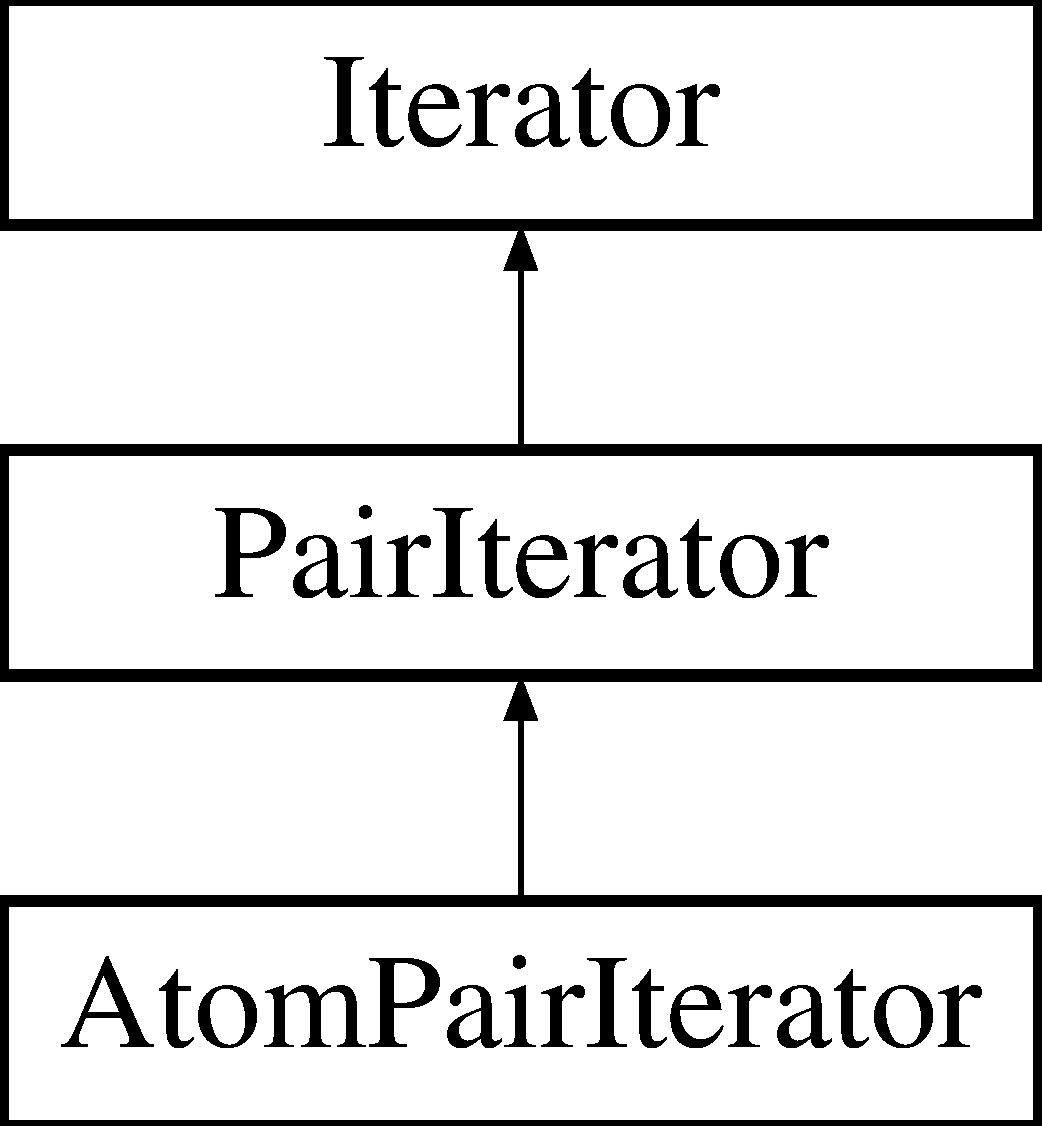
\includegraphics[height=3cm]{classJKBuilder_1_1AtomPairIterator}
\end{center}
\end{figure}
\subsection*{Public Member Functions}
\begin{DoxyCompactItemize}
\item 
\hyperlink{classJKBuilder_1_1AtomPairIterator_a696744d82a9bb3feee21a96f450a510b}{AtomPairIterator} (\hyperlink{classJKBuilder_1_1AtomPairIterator}{AtomPairIterator} const \&other)
\begin{DoxyCompactList}\small\item\em Makes this \hyperlink{classJKBuilder_1_1atom}{atom} pair iterator a copy of other. \item\end{DoxyCompactList}\item 
\hyperlink{classJKBuilder_1_1AtomPairIterator_ad5df59ed812804b6371f17eabeb7d261}{AtomPairIterator} (int NAtoms, bool start)
\begin{DoxyCompactList}\small\item\em if start, makes a new \hyperlink{classJKBuilder_1_1atom}{atom} pair iterator that is ready to iterate, otherwise this is suitable for comparison \item\end{DoxyCompactList}\item 
virtual \hyperlink{classJKBuilder_1_1AtomPairIterator_aa26e88e305008d272c920bf0b959e96b}{$\sim$AtomPairIterator} ()
\item 
bool \hyperlink{classJKBuilder_1_1AtomPairIterator_a1984297ca1081efc0513ec2f5e6a6177}{operator$<$} (\hyperlink{classJKBuilder_1_1PairIterator}{PairIterator} const \&other)
\item 
\hyperlink{classJKBuilder_1_1AtomPairIterator}{AtomPairIterator} \& \hyperlink{classJKBuilder_1_1AtomPairIterator_aefda578091b26523e72740cec884aa45}{operator=} (\hyperlink{classJKBuilder_1_1AtomPairIterator}{AtomPairIterator} const \&other)
\item 
int \hyperlink{classJKBuilder_1_1PairIterator_a370ad37c854fbbf6421ebf9ab35cd027}{ID} (const int i) const 
\begin{DoxyCompactList}\small\item\em Returns the ID of element i of the pair. \item\end{DoxyCompactList}\item 
virtual bool \hyperlink{classJKBuilder_1_1PairIterator_a1984297ca1081efc0513ec2f5e6a6177}{operator$<$} (\hyperlink{classJKBuilder_1_1PairIterator}{PairIterator} const \&other)
\item 
bool \hyperlink{classJKBuilder_1_1PairIterator_a9c95b8dd7929cb34336a944ce96e88a7}{operator$<$=} (\hyperlink{classJKBuilder_1_1PairIterator}{PairIterator} const \&other)
\begin{DoxyCompactList}\small\item\em Returns true if operator$<$ is true or operator== is true. \item\end{DoxyCompactList}\item 
bool \hyperlink{classJKBuilder_1_1PairIterator_ab37a738406950a5e19931f4c09b41f29}{operator$>$} (\hyperlink{classJKBuilder_1_1PairIterator}{PairIterator} const \&other)
\begin{DoxyCompactList}\small\item\em Returns true if operator$<$= is false. \item\end{DoxyCompactList}\item 
bool \hyperlink{classJKBuilder_1_1PairIterator_a0064337d38b8f97d0367be2e9bd31d62}{operator$>$=} (\hyperlink{classJKBuilder_1_1PairIterator}{PairIterator} const \&other)
\begin{DoxyCompactList}\small\item\em Returns true if operator$>$ or operator== is true. \item\end{DoxyCompactList}\item 
bool \hyperlink{classJKBuilder_1_1PairIterator_a6b4e430066f478e5e400edd39ef93968}{operator==} (\hyperlink{classJKBuilder_1_1PairIterator}{PairIterator} const \&other) const 
\item 
virtual void \hyperlink{classJKBuilder_1_1Iterator_a34ca36a99b20ae3170babadaffe51ed2}{Start} (int n=0)
\begin{DoxyCompactList}\small\item\em Returns an iterator suitable for starting on iteration n. \item\end{DoxyCompactList}\item 
virtual void \hyperlink{classJKBuilder_1_1Iterator_a5f692b73d2e160450f4617bb75825e11}{End} (int n=-\/1)
\begin{DoxyCompactList}\small\item\em Returns an iterator representing the state of the iterator after n iterations have occured. \item\end{DoxyCompactList}\item 
\hyperlink{classJKBuilder_1_1Iterator}{Iterator} \hyperlink{classJKBuilder_1_1Iterator_ac1702aedba13b4112b891b58dfd78eba}{operator++} (int)
\begin{DoxyCompactList}\small\item\em Increments the iterator after returning it's value. \item\end{DoxyCompactList}\item 
\hyperlink{classJKBuilder_1_1Iterator}{Iterator} \& \hyperlink{classJKBuilder_1_1Iterator_ae1f21c74128a5ef5d1b9de72ceb09be8}{operator++} ()
\begin{DoxyCompactList}\small\item\em Increments the iterator before returning it's value. \item\end{DoxyCompactList}\item 
bool \hyperlink{classJKBuilder_1_1Iterator_a8c06af8ae0d9d1614ae9f81629275926}{operator!=} (const \hyperlink{classJKBuilder_1_1Iterator}{Iterator} \&other)
\begin{DoxyCompactList}\small\item\em Returns the opposite of operator==. \item\end{DoxyCompactList}\item 
void \hyperlink{classJKBuilder_1_1Iterator_aa83de505e29125c1d3ac7bb1b13ca15a}{SetStart} (std::vector$<$ int $>$ const \&other)
\begin{DoxyCompactList}\small\item\em Sets the N Indices to the N given in other. \item\end{DoxyCompactList}\item 
void \hyperlink{classJKBuilder_1_1Iterator_aad84ec668b5f41210db34c540aaa31fc}{SetEnd} (std::vector$<$ int $>$ const \&other)
\begin{DoxyCompactList}\small\item\em Sets the N MaxInd in other. \item\end{DoxyCompactList}\item 
int \hyperlink{classJKBuilder_1_1Iterator_a74247cf730a06b23fcb1ec64e5596b25}{operator\mbox{[}$\,$\mbox{]}} (const int i) const 
\begin{DoxyCompactList}\small\item\em Returns index i. \item\end{DoxyCompactList}\end{DoxyCompactItemize}
\subsection*{Protected Member Functions}
\begin{DoxyCompactItemize}
\item 
virtual void \hyperlink{classJKBuilder_1_1PairIterator_a7874a07e98b52f4f147cde6f39353bae}{Iterate} ()
\begin{DoxyCompactList}\small\item\em Returns the next valid pair. \item\end{DoxyCompactList}\end{DoxyCompactItemize}
\subsection*{Protected Attributes}
\begin{DoxyCompactItemize}
\item 
int \hyperlink{classJKBuilder_1_1PairIterator_a5c96d22e39dea8044c7caf8c1213e813}{AbsoluteIDs} \mbox{[}2\mbox{]}
\begin{DoxyCompactList}\small\item\em The absolute identity of the system this pair is part of. \item\end{DoxyCompactList}\item 
std::vector$<$ int $>$ \hyperlink{classJKBuilder_1_1Iterator_a20ca24f6d827aba144bb087c4bcb74a0}{CurrentValue}
\begin{DoxyCompactList}\small\item\em The current value. \item\end{DoxyCompactList}\item 
std::vector$<$ int $>$ \hyperlink{classJKBuilder_1_1Iterator_ab6b56d3c4e9353bc938dd6249cde9ca0}{MaxInd}
\begin{DoxyCompactList}\small\item\em This is a vector of length N containing the maximum each index can be. \item\end{DoxyCompactList}\end{DoxyCompactItemize}


\subsection{Detailed Description}
Class to iterate over \hyperlink{classJKBuilder_1_1atom}{atom} pairs in the ERI \hyperlink{classJKBuilder_1_1tensor}{tensor}. 

\subsection{Constructor \& Destructor Documentation}
\hypertarget{classJKBuilder_1_1AtomPairIterator_a696744d82a9bb3feee21a96f450a510b}{
\index{JKBuilder::AtomPairIterator@{JKBuilder::AtomPairIterator}!AtomPairIterator@{AtomPairIterator}}
\index{AtomPairIterator@{AtomPairIterator}!JKBuilder::AtomPairIterator@{JKBuilder::AtomPairIterator}}
\subsubsection[{AtomPairIterator}]{\setlength{\rightskip}{0pt plus 5cm}{\bf AtomPairIterator} ({\bf AtomPairIterator} const \& {\em other})}}
\label{classJKBuilder_1_1AtomPairIterator_a696744d82a9bb3feee21a96f450a510b}


Makes this \hyperlink{classJKBuilder_1_1atom}{atom} pair iterator a copy of other. \hypertarget{classJKBuilder_1_1AtomPairIterator_ad5df59ed812804b6371f17eabeb7d261}{
\index{JKBuilder::AtomPairIterator@{JKBuilder::AtomPairIterator}!AtomPairIterator@{AtomPairIterator}}
\index{AtomPairIterator@{AtomPairIterator}!JKBuilder::AtomPairIterator@{JKBuilder::AtomPairIterator}}
\subsubsection[{AtomPairIterator}]{\setlength{\rightskip}{0pt plus 5cm}{\bf AtomPairIterator} (int {\em NAtoms}, \/  bool {\em start})}}
\label{classJKBuilder_1_1AtomPairIterator_ad5df59ed812804b6371f17eabeb7d261}


if start, makes a new \hyperlink{classJKBuilder_1_1atom}{atom} pair iterator that is ready to iterate, otherwise this is suitable for comparison \hypertarget{classJKBuilder_1_1AtomPairIterator_aa26e88e305008d272c920bf0b959e96b}{
\index{JKBuilder::AtomPairIterator@{JKBuilder::AtomPairIterator}!$\sim$AtomPairIterator@{$\sim$AtomPairIterator}}
\index{$\sim$AtomPairIterator@{$\sim$AtomPairIterator}!JKBuilder::AtomPairIterator@{JKBuilder::AtomPairIterator}}
\subsubsection[{$\sim$AtomPairIterator}]{\setlength{\rightskip}{0pt plus 5cm}$\sim${\bf AtomPairIterator} ()\hspace{0.3cm}{\ttfamily  \mbox{[}virtual\mbox{]}}}}
\label{classJKBuilder_1_1AtomPairIterator_aa26e88e305008d272c920bf0b959e96b}


\subsection{Member Function Documentation}
\hypertarget{classJKBuilder_1_1AtomPairIterator_a1984297ca1081efc0513ec2f5e6a6177}{
\index{JKBuilder::AtomPairIterator@{JKBuilder::AtomPairIterator}!operator$<$@{operator$<$}}
\index{operator$<$@{operator$<$}!JKBuilder::AtomPairIterator@{JKBuilder::AtomPairIterator}}
\subsubsection[{operator$<$}]{\setlength{\rightskip}{0pt plus 5cm}bool operator$<$ ({\bf PairIterator} const \& {\em other})}}
\label{classJKBuilder_1_1AtomPairIterator_a1984297ca1081efc0513ec2f5e6a6177}
\hypertarget{classJKBuilder_1_1AtomPairIterator_aefda578091b26523e72740cec884aa45}{
\index{JKBuilder::AtomPairIterator@{JKBuilder::AtomPairIterator}!operator=@{operator=}}
\index{operator=@{operator=}!JKBuilder::AtomPairIterator@{JKBuilder::AtomPairIterator}}
\subsubsection[{operator=}]{\setlength{\rightskip}{0pt plus 5cm}{\bf AtomPairIterator} \& operator= ({\bf AtomPairIterator} const \& {\em other})}}
\label{classJKBuilder_1_1AtomPairIterator_aefda578091b26523e72740cec884aa45}


Reimplemented from \hyperlink{classJKBuilder_1_1PairIterator_a698aa7b3d6495bd74dcff5b93be868a8}{PairIterator}.\hypertarget{classJKBuilder_1_1PairIterator_a7874a07e98b52f4f147cde6f39353bae}{
\index{JKBuilder::AtomPairIterator@{JKBuilder::AtomPairIterator}!Iterate@{Iterate}}
\index{Iterate@{Iterate}!JKBuilder::AtomPairIterator@{JKBuilder::AtomPairIterator}}
\subsubsection[{Iterate}]{\setlength{\rightskip}{0pt plus 5cm}void Iterate ()\hspace{0.3cm}{\ttfamily  \mbox{[}protected, virtual, inherited\mbox{]}}}}
\label{classJKBuilder_1_1PairIterator_a7874a07e98b52f4f147cde6f39353bae}


Returns the next valid pair. Letting the indices in this pair be P and Q. This returns the next pair that satisfies Q$<$=P 

Reimplemented from \hyperlink{classJKBuilder_1_1Iterator_a7874a07e98b52f4f147cde6f39353bae}{Iterator}.

Reimplemented in \hyperlink{classJKBuilder_1_1ShellPairIterator_a7874a07e98b52f4f147cde6f39353bae}{ShellPairIterator}.\hypertarget{classJKBuilder_1_1PairIterator_a370ad37c854fbbf6421ebf9ab35cd027}{
\index{JKBuilder::AtomPairIterator@{JKBuilder::AtomPairIterator}!ID@{ID}}
\index{ID@{ID}!JKBuilder::AtomPairIterator@{JKBuilder::AtomPairIterator}}
\subsubsection[{ID}]{\setlength{\rightskip}{0pt plus 5cm}int ID (const int {\em i}) const\hspace{0.3cm}{\ttfamily  \mbox{[}inherited\mbox{]}}}}
\label{classJKBuilder_1_1PairIterator_a370ad37c854fbbf6421ebf9ab35cd027}


Returns the ID of element i of the pair. \hypertarget{classJKBuilder_1_1PairIterator_a1984297ca1081efc0513ec2f5e6a6177}{
\index{JKBuilder::AtomPairIterator@{JKBuilder::AtomPairIterator}!operator$<$@{operator$<$}}
\index{operator$<$@{operator$<$}!JKBuilder::AtomPairIterator@{JKBuilder::AtomPairIterator}}
\subsubsection[{operator$<$}]{\setlength{\rightskip}{0pt plus 5cm}bool operator$<$ ({\bf PairIterator} const \& {\em other})\hspace{0.3cm}{\ttfamily  \mbox{[}virtual, inherited\mbox{]}}}}
\label{classJKBuilder_1_1PairIterator_a1984297ca1081efc0513ec2f5e6a6177}
\hypertarget{classJKBuilder_1_1PairIterator_a9c95b8dd7929cb34336a944ce96e88a7}{
\index{JKBuilder::AtomPairIterator@{JKBuilder::AtomPairIterator}!operator$<$=@{operator$<$=}}
\index{operator$<$=@{operator$<$=}!JKBuilder::AtomPairIterator@{JKBuilder::AtomPairIterator}}
\subsubsection[{operator$<$=}]{\setlength{\rightskip}{0pt plus 5cm}bool operator$<$= ({\bf PairIterator} const \& {\em other})\hspace{0.3cm}{\ttfamily  \mbox{[}inherited\mbox{]}}}}
\label{classJKBuilder_1_1PairIterator_a9c95b8dd7929cb34336a944ce96e88a7}


Returns true if operator$<$ is true or operator== is true. \hypertarget{classJKBuilder_1_1PairIterator_ab37a738406950a5e19931f4c09b41f29}{
\index{JKBuilder::AtomPairIterator@{JKBuilder::AtomPairIterator}!operator$>$@{operator$>$}}
\index{operator$>$@{operator$>$}!JKBuilder::AtomPairIterator@{JKBuilder::AtomPairIterator}}
\subsubsection[{operator$>$}]{\setlength{\rightskip}{0pt plus 5cm}bool operator$>$ ({\bf PairIterator} const \& {\em other})\hspace{0.3cm}{\ttfamily  \mbox{[}inherited\mbox{]}}}}
\label{classJKBuilder_1_1PairIterator_ab37a738406950a5e19931f4c09b41f29}


Returns true if operator$<$= is false. \hypertarget{classJKBuilder_1_1PairIterator_a0064337d38b8f97d0367be2e9bd31d62}{
\index{JKBuilder::AtomPairIterator@{JKBuilder::AtomPairIterator}!operator$>$=@{operator$>$=}}
\index{operator$>$=@{operator$>$=}!JKBuilder::AtomPairIterator@{JKBuilder::AtomPairIterator}}
\subsubsection[{operator$>$=}]{\setlength{\rightskip}{0pt plus 5cm}bool operator$>$= ({\bf PairIterator} const \& {\em other})\hspace{0.3cm}{\ttfamily  \mbox{[}inherited\mbox{]}}}}
\label{classJKBuilder_1_1PairIterator_a0064337d38b8f97d0367be2e9bd31d62}


Returns true if operator$>$ or operator== is true. \hypertarget{classJKBuilder_1_1PairIterator_a6b4e430066f478e5e400edd39ef93968}{
\index{JKBuilder::AtomPairIterator@{JKBuilder::AtomPairIterator}!operator==@{operator==}}
\index{operator==@{operator==}!JKBuilder::AtomPairIterator@{JKBuilder::AtomPairIterator}}
\subsubsection[{operator==}]{\setlength{\rightskip}{0pt plus 5cm}bool operator== ({\bf PairIterator} const \& {\em other}) const\hspace{0.3cm}{\ttfamily  \mbox{[}inherited\mbox{]}}}}
\label{classJKBuilder_1_1PairIterator_a6b4e430066f478e5e400edd39ef93968}


Reimplemented from \hyperlink{classJKBuilder_1_1Iterator_a1ea001976a5bc8ae8dc365e2a912b59a}{Iterator}.\hypertarget{classJKBuilder_1_1Iterator_a34ca36a99b20ae3170babadaffe51ed2}{
\index{JKBuilder::AtomPairIterator@{JKBuilder::AtomPairIterator}!Start@{Start}}
\index{Start@{Start}!JKBuilder::AtomPairIterator@{JKBuilder::AtomPairIterator}}
\subsubsection[{Start}]{\setlength{\rightskip}{0pt plus 5cm}void Start (int {\em n} = {\ttfamily 0})\hspace{0.3cm}{\ttfamily  \mbox{[}virtual, inherited\mbox{]}}}}
\label{classJKBuilder_1_1Iterator_a34ca36a99b20ae3170babadaffe51ed2}


Returns an iterator suitable for starting on iteration n. 

Reimplemented in \hyperlink{classJKBuilder_1_1QuartetIterator_a34ca36a99b20ae3170babadaffe51ed2}{QuartetIterator}.\hypertarget{classJKBuilder_1_1Iterator_a5f692b73d2e160450f4617bb75825e11}{
\index{JKBuilder::AtomPairIterator@{JKBuilder::AtomPairIterator}!End@{End}}
\index{End@{End}!JKBuilder::AtomPairIterator@{JKBuilder::AtomPairIterator}}
\subsubsection[{End}]{\setlength{\rightskip}{0pt plus 5cm}void End (int {\em n} = {\ttfamily -\/1})\hspace{0.3cm}{\ttfamily  \mbox{[}virtual, inherited\mbox{]}}}}
\label{classJKBuilder_1_1Iterator_a5f692b73d2e160450f4617bb75825e11}


Returns an iterator representing the state of the iterator after n iterations have occured. The default argument is n=-\/1, which is a flag corresponding to the last iteration of the iterator 

Reimplemented in \hyperlink{classJKBuilder_1_1QuartetIterator_a5f692b73d2e160450f4617bb75825e11}{QuartetIterator}.\hypertarget{classJKBuilder_1_1Iterator_ac1702aedba13b4112b891b58dfd78eba}{
\index{JKBuilder::AtomPairIterator@{JKBuilder::AtomPairIterator}!operator++@{operator++}}
\index{operator++@{operator++}!JKBuilder::AtomPairIterator@{JKBuilder::AtomPairIterator}}
\subsubsection[{operator++}]{\setlength{\rightskip}{0pt plus 5cm}{\bf Iterator} operator++ (int)\hspace{0.3cm}{\ttfamily  \mbox{[}inherited\mbox{]}}}}
\label{classJKBuilder_1_1Iterator_ac1702aedba13b4112b891b58dfd78eba}


Increments the iterator after returning it's value. \hypertarget{classJKBuilder_1_1Iterator_ae1f21c74128a5ef5d1b9de72ceb09be8}{
\index{JKBuilder::AtomPairIterator@{JKBuilder::AtomPairIterator}!operator++@{operator++}}
\index{operator++@{operator++}!JKBuilder::AtomPairIterator@{JKBuilder::AtomPairIterator}}
\subsubsection[{operator++}]{\setlength{\rightskip}{0pt plus 5cm}{\bf Iterator} \& operator++ ()\hspace{0.3cm}{\ttfamily  \mbox{[}inherited\mbox{]}}}}
\label{classJKBuilder_1_1Iterator_ae1f21c74128a5ef5d1b9de72ceb09be8}


Increments the iterator before returning it's value. \hypertarget{classJKBuilder_1_1Iterator_a8c06af8ae0d9d1614ae9f81629275926}{
\index{JKBuilder::AtomPairIterator@{JKBuilder::AtomPairIterator}!operator!=@{operator!=}}
\index{operator!=@{operator!=}!JKBuilder::AtomPairIterator@{JKBuilder::AtomPairIterator}}
\subsubsection[{operator!=}]{\setlength{\rightskip}{0pt plus 5cm}bool operator!= (const {\bf Iterator} \& {\em other})\hspace{0.3cm}{\ttfamily  \mbox{[}inherited\mbox{]}}}}
\label{classJKBuilder_1_1Iterator_a8c06af8ae0d9d1614ae9f81629275926}


Returns the opposite of operator==. \hypertarget{classJKBuilder_1_1Iterator_aa83de505e29125c1d3ac7bb1b13ca15a}{
\index{JKBuilder::AtomPairIterator@{JKBuilder::AtomPairIterator}!SetStart@{SetStart}}
\index{SetStart@{SetStart}!JKBuilder::AtomPairIterator@{JKBuilder::AtomPairIterator}}
\subsubsection[{SetStart}]{\setlength{\rightskip}{0pt plus 5cm}void SetStart (std::vector$<$ int $>$ const \& {\em other})\hspace{0.3cm}{\ttfamily  \mbox{[}inherited\mbox{]}}}}
\label{classJKBuilder_1_1Iterator_aa83de505e29125c1d3ac7bb1b13ca15a}


Sets the N Indices to the N given in other. \hypertarget{classJKBuilder_1_1Iterator_aad84ec668b5f41210db34c540aaa31fc}{
\index{JKBuilder::AtomPairIterator@{JKBuilder::AtomPairIterator}!SetEnd@{SetEnd}}
\index{SetEnd@{SetEnd}!JKBuilder::AtomPairIterator@{JKBuilder::AtomPairIterator}}
\subsubsection[{SetEnd}]{\setlength{\rightskip}{0pt plus 5cm}void SetEnd (std::vector$<$ int $>$ const \& {\em other})\hspace{0.3cm}{\ttfamily  \mbox{[}inherited\mbox{]}}}}
\label{classJKBuilder_1_1Iterator_aad84ec668b5f41210db34c540aaa31fc}


Sets the N MaxInd in other. \hypertarget{classJKBuilder_1_1Iterator_a74247cf730a06b23fcb1ec64e5596b25}{
\index{JKBuilder::AtomPairIterator@{JKBuilder::AtomPairIterator}!operator\mbox{[}\mbox{]}@{operator[]}}
\index{operator\mbox{[}\mbox{]}@{operator[]}!JKBuilder::AtomPairIterator@{JKBuilder::AtomPairIterator}}
\subsubsection[{operator[]}]{\setlength{\rightskip}{0pt plus 5cm}int operator\mbox{[}$\,$\mbox{]} (const int {\em i}) const\hspace{0.3cm}{\ttfamily  \mbox{[}inherited\mbox{]}}}}
\label{classJKBuilder_1_1Iterator_a74247cf730a06b23fcb1ec64e5596b25}


Returns index i. 

\subsection{Member Data Documentation}
\hypertarget{classJKBuilder_1_1PairIterator_a5c96d22e39dea8044c7caf8c1213e813}{
\index{JKBuilder::AtomPairIterator@{JKBuilder::AtomPairIterator}!AbsoluteIDs@{AbsoluteIDs}}
\index{AbsoluteIDs@{AbsoluteIDs}!JKBuilder::AtomPairIterator@{JKBuilder::AtomPairIterator}}
\subsubsection[{AbsoluteIDs}]{\setlength{\rightskip}{0pt plus 5cm}int {\bf AbsoluteIDs}\mbox{[}2\mbox{]}\hspace{0.3cm}{\ttfamily  \mbox{[}protected, inherited\mbox{]}}}}
\label{classJKBuilder_1_1PairIterator_a5c96d22e39dea8044c7caf8c1213e813}


The absolute identity of the system this pair is part of. If this is a pair of atoms set all elements of this to 0 (all atoms are part of the same molecule. If this is a pair of shells set it to the identity of the \hyperlink{classJKBuilder_1_1atom}{atom} the shell is on. \hypertarget{classJKBuilder_1_1Iterator_a20ca24f6d827aba144bb087c4bcb74a0}{
\index{JKBuilder::AtomPairIterator@{JKBuilder::AtomPairIterator}!CurrentValue@{CurrentValue}}
\index{CurrentValue@{CurrentValue}!JKBuilder::AtomPairIterator@{JKBuilder::AtomPairIterator}}
\subsubsection[{CurrentValue}]{\setlength{\rightskip}{0pt plus 5cm}std::vector$<$int$>$ {\bf CurrentValue}\hspace{0.3cm}{\ttfamily  \mbox{[}protected, inherited\mbox{]}}}}
\label{classJKBuilder_1_1Iterator_a20ca24f6d827aba144bb087c4bcb74a0}


The current value. \hypertarget{classJKBuilder_1_1Iterator_ab6b56d3c4e9353bc938dd6249cde9ca0}{
\index{JKBuilder::AtomPairIterator@{JKBuilder::AtomPairIterator}!MaxInd@{MaxInd}}
\index{MaxInd@{MaxInd}!JKBuilder::AtomPairIterator@{JKBuilder::AtomPairIterator}}
\subsubsection[{MaxInd}]{\setlength{\rightskip}{0pt plus 5cm}std::vector$<$int$>$ {\bf MaxInd}\hspace{0.3cm}{\ttfamily  \mbox{[}protected, inherited\mbox{]}}}}
\label{classJKBuilder_1_1Iterator_ab6b56d3c4e9353bc938dd6249cde9ca0}


This is a vector of length N containing the maximum each index can be. 

The documentation for this class was generated from the following files:\begin{DoxyCompactItemize}
\item 
src/\hyperlink{Iterators_8h}{Iterators.h}\item 
src/\hyperlink{Iterator_8cpp}{Iterator.cpp}\end{DoxyCompactItemize}

\hypertarget{classJKBuilder_1_1AtomQuartetIterator}{
\section{AtomQuartetIterator Class Reference}
\label{classJKBuilder_1_1AtomQuartetIterator}\index{JKBuilder::AtomQuartetIterator@{JKBuilder::AtomQuartetIterator}}
}


Iterates over pairs of Atom pairs.  


{\ttfamily \#include $<$Iterators.h$>$}Inheritance diagram for AtomQuartetIterator::\begin{figure}[H]
\begin{center}
\leavevmode
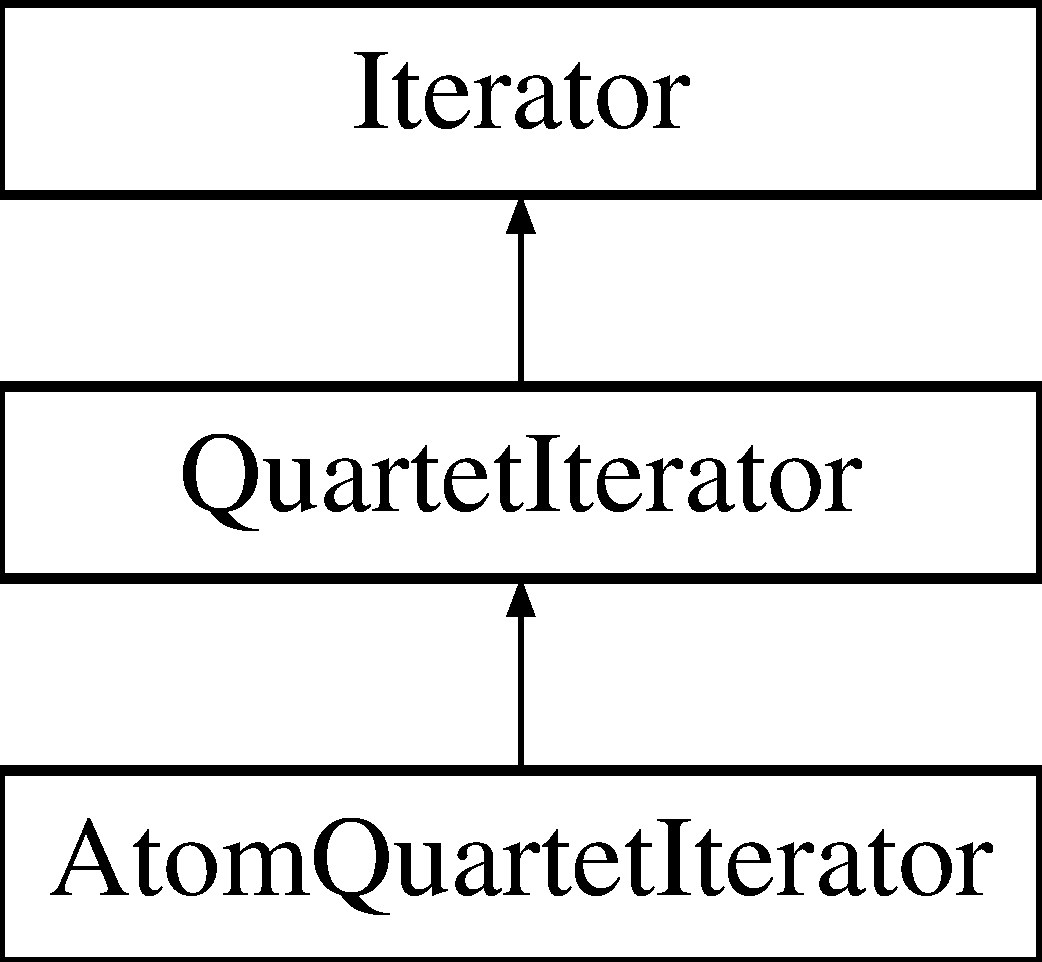
\includegraphics[height=3cm]{classJKBuilder_1_1AtomQuartetIterator}
\end{center}
\end{figure}
\subsection*{Public Member Functions}
\begin{DoxyCompactItemize}
\item 
\hyperlink{classJKBuilder_1_1AtomQuartetIterator_ab6c4f20fcdd55b5e65bd25fd0ffa6aab}{AtomQuartetIterator} (\hyperlink{classJKBuilder_1_1AtomQuartetIterator}{AtomQuartetIterator} const \&other)
\begin{DoxyCompactList}\small\item\em Makes this iterator a copy of another one. \item\end{DoxyCompactList}\item 
\hyperlink{classJKBuilder_1_1AtomQuartetIterator_a9cf8914af3c8623ae212e03307e27195}{AtomQuartetIterator} (int NAtoms, bool start)
\begin{DoxyCompactList}\small\item\em Makes an iterator for pairs of pairs of atoms, chosen from NAtoms (if start==true) or the end condition (start==false). \item\end{DoxyCompactList}\item 
\hyperlink{classJKBuilder_1_1AtomQuartetIterator}{AtomQuartetIterator} \& \hyperlink{classJKBuilder_1_1AtomQuartetIterator_a39f50a07009d2e9e81e1d64da594084f}{operator=} (\hyperlink{classJKBuilder_1_1AtomQuartetIterator}{AtomQuartetIterator} const \&other)
\item 
void \hyperlink{classJKBuilder_1_1QuartetIterator_a34ca36a99b20ae3170babadaffe51ed2}{Start} (int n=0)
\begin{DoxyCompactList}\small\item\em Returns an iterator suitable for starting on iteration n. \item\end{DoxyCompactList}\item 
void \hyperlink{classJKBuilder_1_1QuartetIterator_a5f692b73d2e160450f4617bb75825e11}{End} (int n=-\/1)
\begin{DoxyCompactList}\small\item\em Returns an iterator representing the state of the iterator after n iterations have occured. \item\end{DoxyCompactList}\item 
\hyperlink{classJKBuilder_1_1Iterator}{Iterator} \hyperlink{classJKBuilder_1_1Iterator_ac1702aedba13b4112b891b58dfd78eba}{operator++} (int)
\begin{DoxyCompactList}\small\item\em Increments the iterator after returning it's value. \item\end{DoxyCompactList}\item 
\hyperlink{classJKBuilder_1_1Iterator}{Iterator} \& \hyperlink{classJKBuilder_1_1Iterator_ae1f21c74128a5ef5d1b9de72ceb09be8}{operator++} ()
\begin{DoxyCompactList}\small\item\em Increments the iterator before returning it's value. \item\end{DoxyCompactList}\item 
bool \hyperlink{classJKBuilder_1_1Iterator_a1ea001976a5bc8ae8dc365e2a912b59a}{operator==} (const \hyperlink{classJKBuilder_1_1Iterator}{Iterator} \&other) const 
\item 
bool \hyperlink{classJKBuilder_1_1Iterator_a8c06af8ae0d9d1614ae9f81629275926}{operator!=} (const \hyperlink{classJKBuilder_1_1Iterator}{Iterator} \&other)
\begin{DoxyCompactList}\small\item\em Returns the opposite of operator==. \item\end{DoxyCompactList}\item 
void \hyperlink{classJKBuilder_1_1Iterator_aa83de505e29125c1d3ac7bb1b13ca15a}{SetStart} (std::vector$<$ int $>$ const \&other)
\begin{DoxyCompactList}\small\item\em Sets the N Indices to the N given in other. \item\end{DoxyCompactList}\item 
void \hyperlink{classJKBuilder_1_1Iterator_aad84ec668b5f41210db34c540aaa31fc}{SetEnd} (std::vector$<$ int $>$ const \&other)
\begin{DoxyCompactList}\small\item\em Sets the N MaxInd in other. \item\end{DoxyCompactList}\item 
int \hyperlink{classJKBuilder_1_1Iterator_a74247cf730a06b23fcb1ec64e5596b25}{operator\mbox{[}$\,$\mbox{]}} (const int i) const 
\begin{DoxyCompactList}\small\item\em Returns index i. \item\end{DoxyCompactList}\end{DoxyCompactItemize}
\subsection*{Protected Member Functions}
\begin{DoxyCompactItemize}
\item 
bool \hyperlink{classJKBuilder_1_1AtomQuartetIterator_a458dcf49c4c4bbb1e3d3d39d3dc086c9}{RSIsMaxed} ()
\begin{DoxyCompactList}\small\item\em The definition of what it means for RS to be maxed. \item\end{DoxyCompactList}\item 
bool \hyperlink{classJKBuilder_1_1AtomQuartetIterator_a13e657ea529c0566a0bf48e9c5a488d7}{RSIsOK} ()
\begin{DoxyCompactList}\small\item\em A check to see if the iterated RS value is acceptable. \item\end{DoxyCompactList}\item 
virtual void \hyperlink{classJKBuilder_1_1QuartetIterator_a7874a07e98b52f4f147cde6f39353bae}{Iterate} ()
\item 
void \hyperlink{classJKBuilder_1_1QuartetIterator_a1af5c865d6e9cfe63d0dedc53bdc13ba}{UpdateCurrentValue} ()
\begin{DoxyCompactList}\small\item\em Copies PQ and RS into CurrentValue. \item\end{DoxyCompactList}\end{DoxyCompactItemize}
\subsection*{Protected Attributes}
\begin{DoxyCompactItemize}
\item 
\hyperlink{classJKBuilder_1_1PairIterator}{PairIterator} $\ast$ \hyperlink{classJKBuilder_1_1QuartetIterator_a84f5c3632fba19d3bb85e1cffb9e51f7}{PQ}
\item 
\hyperlink{classJKBuilder_1_1PairIterator}{PairIterator} $\ast$ \hyperlink{classJKBuilder_1_1QuartetIterator_a26b777bf7ea22524f1cc725020ee2082}{RS}
\item 
std::vector$<$ int $>$ \hyperlink{classJKBuilder_1_1Iterator_a20ca24f6d827aba144bb087c4bcb74a0}{CurrentValue}
\begin{DoxyCompactList}\small\item\em The current value. \item\end{DoxyCompactList}\item 
std::vector$<$ int $>$ \hyperlink{classJKBuilder_1_1Iterator_ab6b56d3c4e9353bc938dd6249cde9ca0}{MaxInd}
\begin{DoxyCompactList}\small\item\em This is a vector of length N containing the maximum each index can be. \item\end{DoxyCompactList}\end{DoxyCompactItemize}


\subsection{Detailed Description}
Iterates over pairs of Atom pairs. 

\subsection{Constructor \& Destructor Documentation}
\hypertarget{classJKBuilder_1_1AtomQuartetIterator_ab6c4f20fcdd55b5e65bd25fd0ffa6aab}{
\index{JKBuilder::AtomQuartetIterator@{JKBuilder::AtomQuartetIterator}!AtomQuartetIterator@{AtomQuartetIterator}}
\index{AtomQuartetIterator@{AtomQuartetIterator}!JKBuilder::AtomQuartetIterator@{JKBuilder::AtomQuartetIterator}}
\subsubsection[{AtomQuartetIterator}]{\setlength{\rightskip}{0pt plus 5cm}{\bf AtomQuartetIterator} ({\bf AtomQuartetIterator} const \& {\em other})}}
\label{classJKBuilder_1_1AtomQuartetIterator_ab6c4f20fcdd55b5e65bd25fd0ffa6aab}


Makes this iterator a copy of another one. \hypertarget{classJKBuilder_1_1AtomQuartetIterator_a9cf8914af3c8623ae212e03307e27195}{
\index{JKBuilder::AtomQuartetIterator@{JKBuilder::AtomQuartetIterator}!AtomQuartetIterator@{AtomQuartetIterator}}
\index{AtomQuartetIterator@{AtomQuartetIterator}!JKBuilder::AtomQuartetIterator@{JKBuilder::AtomQuartetIterator}}
\subsubsection[{AtomQuartetIterator}]{\setlength{\rightskip}{0pt plus 5cm}{\bf AtomQuartetIterator} (int {\em NAtoms}, \/  bool {\em start})}}
\label{classJKBuilder_1_1AtomQuartetIterator_a9cf8914af3c8623ae212e03307e27195}


Makes an iterator for pairs of pairs of atoms, chosen from NAtoms (if start==true) or the end condition (start==false). 

\subsection{Member Function Documentation}
\hypertarget{classJKBuilder_1_1AtomQuartetIterator_a458dcf49c4c4bbb1e3d3d39d3dc086c9}{
\index{JKBuilder::AtomQuartetIterator@{JKBuilder::AtomQuartetIterator}!RSIsMaxed@{RSIsMaxed}}
\index{RSIsMaxed@{RSIsMaxed}!JKBuilder::AtomQuartetIterator@{JKBuilder::AtomQuartetIterator}}
\subsubsection[{RSIsMaxed}]{\setlength{\rightskip}{0pt plus 5cm}bool RSIsMaxed ()\hspace{0.3cm}{\ttfamily  \mbox{[}protected, virtual\mbox{]}}}}
\label{classJKBuilder_1_1AtomQuartetIterator_a458dcf49c4c4bbb1e3d3d39d3dc086c9}


The definition of what it means for RS to be maxed. 

Implements \hyperlink{classJKBuilder_1_1QuartetIterator_af88c46759ac710bbd36c17601dc62d55}{QuartetIterator}.\hypertarget{classJKBuilder_1_1AtomQuartetIterator_a13e657ea529c0566a0bf48e9c5a488d7}{
\index{JKBuilder::AtomQuartetIterator@{JKBuilder::AtomQuartetIterator}!RSIsOK@{RSIsOK}}
\index{RSIsOK@{RSIsOK}!JKBuilder::AtomQuartetIterator@{JKBuilder::AtomQuartetIterator}}
\subsubsection[{RSIsOK}]{\setlength{\rightskip}{0pt plus 5cm}bool RSIsOK ()\hspace{0.3cm}{\ttfamily  \mbox{[}protected, virtual\mbox{]}}}}
\label{classJKBuilder_1_1AtomQuartetIterator_a13e657ea529c0566a0bf48e9c5a488d7}


A check to see if the iterated RS value is acceptable. 

Implements \hyperlink{classJKBuilder_1_1QuartetIterator_ac51ff9a02f4a201598f7820476c52faf}{QuartetIterator}.\hypertarget{classJKBuilder_1_1AtomQuartetIterator_a39f50a07009d2e9e81e1d64da594084f}{
\index{JKBuilder::AtomQuartetIterator@{JKBuilder::AtomQuartetIterator}!operator=@{operator=}}
\index{operator=@{operator=}!JKBuilder::AtomQuartetIterator@{JKBuilder::AtomQuartetIterator}}
\subsubsection[{operator=}]{\setlength{\rightskip}{0pt plus 5cm}{\bf AtomQuartetIterator} \& operator= ({\bf AtomQuartetIterator} const \& {\em other})}}
\label{classJKBuilder_1_1AtomQuartetIterator_a39f50a07009d2e9e81e1d64da594084f}


Reimplemented from \hyperlink{classJKBuilder_1_1QuartetIterator_ab3cd17222545586596dbbc6aa3ca7046}{QuartetIterator}.\hypertarget{classJKBuilder_1_1QuartetIterator_a7874a07e98b52f4f147cde6f39353bae}{
\index{JKBuilder::AtomQuartetIterator@{JKBuilder::AtomQuartetIterator}!Iterate@{Iterate}}
\index{Iterate@{Iterate}!JKBuilder::AtomQuartetIterator@{JKBuilder::AtomQuartetIterator}}
\subsubsection[{Iterate}]{\setlength{\rightskip}{0pt plus 5cm}void Iterate ()\hspace{0.3cm}{\ttfamily  \mbox{[}protected, virtual, inherited\mbox{]}}}}
\label{classJKBuilder_1_1QuartetIterator_a7874a07e98b52f4f147cde6f39353bae}


Reimplemented from \hyperlink{classJKBuilder_1_1Iterator_a7874a07e98b52f4f147cde6f39353bae}{Iterator}.\hypertarget{classJKBuilder_1_1QuartetIterator_a1af5c865d6e9cfe63d0dedc53bdc13ba}{
\index{JKBuilder::AtomQuartetIterator@{JKBuilder::AtomQuartetIterator}!UpdateCurrentValue@{UpdateCurrentValue}}
\index{UpdateCurrentValue@{UpdateCurrentValue}!JKBuilder::AtomQuartetIterator@{JKBuilder::AtomQuartetIterator}}
\subsubsection[{UpdateCurrentValue}]{\setlength{\rightskip}{0pt plus 5cm}void UpdateCurrentValue ()\hspace{0.3cm}{\ttfamily  \mbox{[}protected, inherited\mbox{]}}}}
\label{classJKBuilder_1_1QuartetIterator_a1af5c865d6e9cfe63d0dedc53bdc13ba}


Copies PQ and RS into CurrentValue. \hypertarget{classJKBuilder_1_1QuartetIterator_a34ca36a99b20ae3170babadaffe51ed2}{
\index{JKBuilder::AtomQuartetIterator@{JKBuilder::AtomQuartetIterator}!Start@{Start}}
\index{Start@{Start}!JKBuilder::AtomQuartetIterator@{JKBuilder::AtomQuartetIterator}}
\subsubsection[{Start}]{\setlength{\rightskip}{0pt plus 5cm}void Start (int {\em n} = {\ttfamily 0})\hspace{0.3cm}{\ttfamily  \mbox{[}virtual, inherited\mbox{]}}}}
\label{classJKBuilder_1_1QuartetIterator_a34ca36a99b20ae3170babadaffe51ed2}


Returns an iterator suitable for starting on iteration n. 

Reimplemented from \hyperlink{classJKBuilder_1_1Iterator_a34ca36a99b20ae3170babadaffe51ed2}{Iterator}.\hypertarget{classJKBuilder_1_1QuartetIterator_a5f692b73d2e160450f4617bb75825e11}{
\index{JKBuilder::AtomQuartetIterator@{JKBuilder::AtomQuartetIterator}!End@{End}}
\index{End@{End}!JKBuilder::AtomQuartetIterator@{JKBuilder::AtomQuartetIterator}}
\subsubsection[{End}]{\setlength{\rightskip}{0pt plus 5cm}void End (int {\em n} = {\ttfamily -\/1})\hspace{0.3cm}{\ttfamily  \mbox{[}virtual, inherited\mbox{]}}}}
\label{classJKBuilder_1_1QuartetIterator_a5f692b73d2e160450f4617bb75825e11}


Returns an iterator representing the state of the iterator after n iterations have occured. The default argument is n=-\/1, which is a flag corresponding to the last iteration of the iterator 

Reimplemented from \hyperlink{classJKBuilder_1_1Iterator_a5f692b73d2e160450f4617bb75825e11}{Iterator}.\hypertarget{classJKBuilder_1_1Iterator_ac1702aedba13b4112b891b58dfd78eba}{
\index{JKBuilder::AtomQuartetIterator@{JKBuilder::AtomQuartetIterator}!operator++@{operator++}}
\index{operator++@{operator++}!JKBuilder::AtomQuartetIterator@{JKBuilder::AtomQuartetIterator}}
\subsubsection[{operator++}]{\setlength{\rightskip}{0pt plus 5cm}{\bf Iterator} operator++ (int)\hspace{0.3cm}{\ttfamily  \mbox{[}inherited\mbox{]}}}}
\label{classJKBuilder_1_1Iterator_ac1702aedba13b4112b891b58dfd78eba}


Increments the iterator after returning it's value. \hypertarget{classJKBuilder_1_1Iterator_ae1f21c74128a5ef5d1b9de72ceb09be8}{
\index{JKBuilder::AtomQuartetIterator@{JKBuilder::AtomQuartetIterator}!operator++@{operator++}}
\index{operator++@{operator++}!JKBuilder::AtomQuartetIterator@{JKBuilder::AtomQuartetIterator}}
\subsubsection[{operator++}]{\setlength{\rightskip}{0pt plus 5cm}{\bf Iterator} \& operator++ ()\hspace{0.3cm}{\ttfamily  \mbox{[}inherited\mbox{]}}}}
\label{classJKBuilder_1_1Iterator_ae1f21c74128a5ef5d1b9de72ceb09be8}


Increments the iterator before returning it's value. \hypertarget{classJKBuilder_1_1Iterator_a1ea001976a5bc8ae8dc365e2a912b59a}{
\index{JKBuilder::AtomQuartetIterator@{JKBuilder::AtomQuartetIterator}!operator==@{operator==}}
\index{operator==@{operator==}!JKBuilder::AtomQuartetIterator@{JKBuilder::AtomQuartetIterator}}
\subsubsection[{operator==}]{\setlength{\rightskip}{0pt plus 5cm}bool operator== (const {\bf Iterator} \& {\em other}) const\hspace{0.3cm}{\ttfamily  \mbox{[}inherited\mbox{]}}}}
\label{classJKBuilder_1_1Iterator_a1ea001976a5bc8ae8dc365e2a912b59a}


Reimplemented in \hyperlink{classJKBuilder_1_1PairIterator_a6b4e430066f478e5e400edd39ef93968}{PairIterator}.\hypertarget{classJKBuilder_1_1Iterator_a8c06af8ae0d9d1614ae9f81629275926}{
\index{JKBuilder::AtomQuartetIterator@{JKBuilder::AtomQuartetIterator}!operator!=@{operator!=}}
\index{operator!=@{operator!=}!JKBuilder::AtomQuartetIterator@{JKBuilder::AtomQuartetIterator}}
\subsubsection[{operator!=}]{\setlength{\rightskip}{0pt plus 5cm}bool operator!= (const {\bf Iterator} \& {\em other})\hspace{0.3cm}{\ttfamily  \mbox{[}inherited\mbox{]}}}}
\label{classJKBuilder_1_1Iterator_a8c06af8ae0d9d1614ae9f81629275926}


Returns the opposite of operator==. \hypertarget{classJKBuilder_1_1Iterator_aa83de505e29125c1d3ac7bb1b13ca15a}{
\index{JKBuilder::AtomQuartetIterator@{JKBuilder::AtomQuartetIterator}!SetStart@{SetStart}}
\index{SetStart@{SetStart}!JKBuilder::AtomQuartetIterator@{JKBuilder::AtomQuartetIterator}}
\subsubsection[{SetStart}]{\setlength{\rightskip}{0pt plus 5cm}void SetStart (std::vector$<$ int $>$ const \& {\em other})\hspace{0.3cm}{\ttfamily  \mbox{[}inherited\mbox{]}}}}
\label{classJKBuilder_1_1Iterator_aa83de505e29125c1d3ac7bb1b13ca15a}


Sets the N Indices to the N given in other. \hypertarget{classJKBuilder_1_1Iterator_aad84ec668b5f41210db34c540aaa31fc}{
\index{JKBuilder::AtomQuartetIterator@{JKBuilder::AtomQuartetIterator}!SetEnd@{SetEnd}}
\index{SetEnd@{SetEnd}!JKBuilder::AtomQuartetIterator@{JKBuilder::AtomQuartetIterator}}
\subsubsection[{SetEnd}]{\setlength{\rightskip}{0pt plus 5cm}void SetEnd (std::vector$<$ int $>$ const \& {\em other})\hspace{0.3cm}{\ttfamily  \mbox{[}inherited\mbox{]}}}}
\label{classJKBuilder_1_1Iterator_aad84ec668b5f41210db34c540aaa31fc}


Sets the N MaxInd in other. \hypertarget{classJKBuilder_1_1Iterator_a74247cf730a06b23fcb1ec64e5596b25}{
\index{JKBuilder::AtomQuartetIterator@{JKBuilder::AtomQuartetIterator}!operator\mbox{[}\mbox{]}@{operator[]}}
\index{operator\mbox{[}\mbox{]}@{operator[]}!JKBuilder::AtomQuartetIterator@{JKBuilder::AtomQuartetIterator}}
\subsubsection[{operator[]}]{\setlength{\rightskip}{0pt plus 5cm}int operator\mbox{[}$\,$\mbox{]} (const int {\em i}) const\hspace{0.3cm}{\ttfamily  \mbox{[}inherited\mbox{]}}}}
\label{classJKBuilder_1_1Iterator_a74247cf730a06b23fcb1ec64e5596b25}


Returns index i. 

\subsection{Member Data Documentation}
\hypertarget{classJKBuilder_1_1QuartetIterator_a84f5c3632fba19d3bb85e1cffb9e51f7}{
\index{JKBuilder::AtomQuartetIterator@{JKBuilder::AtomQuartetIterator}!PQ@{PQ}}
\index{PQ@{PQ}!JKBuilder::AtomQuartetIterator@{JKBuilder::AtomQuartetIterator}}
\subsubsection[{PQ}]{\setlength{\rightskip}{0pt plus 5cm}{\bf PairIterator}$\ast$ {\bf PQ}\hspace{0.3cm}{\ttfamily  \mbox{[}protected, inherited\mbox{]}}}}
\label{classJKBuilder_1_1QuartetIterator_a84f5c3632fba19d3bb85e1cffb9e51f7}
\hypertarget{classJKBuilder_1_1QuartetIterator_a26b777bf7ea22524f1cc725020ee2082}{
\index{JKBuilder::AtomQuartetIterator@{JKBuilder::AtomQuartetIterator}!RS@{RS}}
\index{RS@{RS}!JKBuilder::AtomQuartetIterator@{JKBuilder::AtomQuartetIterator}}
\subsubsection[{RS}]{\setlength{\rightskip}{0pt plus 5cm}{\bf PairIterator}$\ast$ {\bf RS}\hspace{0.3cm}{\ttfamily  \mbox{[}protected, inherited\mbox{]}}}}
\label{classJKBuilder_1_1QuartetIterator_a26b777bf7ea22524f1cc725020ee2082}
\hypertarget{classJKBuilder_1_1Iterator_a20ca24f6d827aba144bb087c4bcb74a0}{
\index{JKBuilder::AtomQuartetIterator@{JKBuilder::AtomQuartetIterator}!CurrentValue@{CurrentValue}}
\index{CurrentValue@{CurrentValue}!JKBuilder::AtomQuartetIterator@{JKBuilder::AtomQuartetIterator}}
\subsubsection[{CurrentValue}]{\setlength{\rightskip}{0pt plus 5cm}std::vector$<$int$>$ {\bf CurrentValue}\hspace{0.3cm}{\ttfamily  \mbox{[}protected, inherited\mbox{]}}}}
\label{classJKBuilder_1_1Iterator_a20ca24f6d827aba144bb087c4bcb74a0}


The current value. \hypertarget{classJKBuilder_1_1Iterator_ab6b56d3c4e9353bc938dd6249cde9ca0}{
\index{JKBuilder::AtomQuartetIterator@{JKBuilder::AtomQuartetIterator}!MaxInd@{MaxInd}}
\index{MaxInd@{MaxInd}!JKBuilder::AtomQuartetIterator@{JKBuilder::AtomQuartetIterator}}
\subsubsection[{MaxInd}]{\setlength{\rightskip}{0pt plus 5cm}std::vector$<$int$>$ {\bf MaxInd}\hspace{0.3cm}{\ttfamily  \mbox{[}protected, inherited\mbox{]}}}}
\label{classJKBuilder_1_1Iterator_ab6b56d3c4e9353bc938dd6249cde9ca0}


This is a vector of length N containing the maximum each index can be. 

The documentation for this class was generated from the following files:\begin{DoxyCompactItemize}
\item 
src/\hyperlink{Iterators_8h}{Iterators.h}\item 
src/\hyperlink{Iterator_8cpp}{Iterator.cpp}\end{DoxyCompactItemize}

\hypertarget{classJKBuilder_1_1BasisQuartetIterator}{
\section{BasisQuartetIterator Class Reference}
\label{classJKBuilder_1_1BasisQuartetIterator}\index{JKBuilder::BasisQuartetIterator@{JKBuilder::BasisQuartetIterator}}
}


Iterates over the BasisPairs.  


{\ttfamily \#include $<$Iterators.h$>$}Inheritance diagram for BasisQuartetIterator::\begin{figure}[H]
\begin{center}
\leavevmode
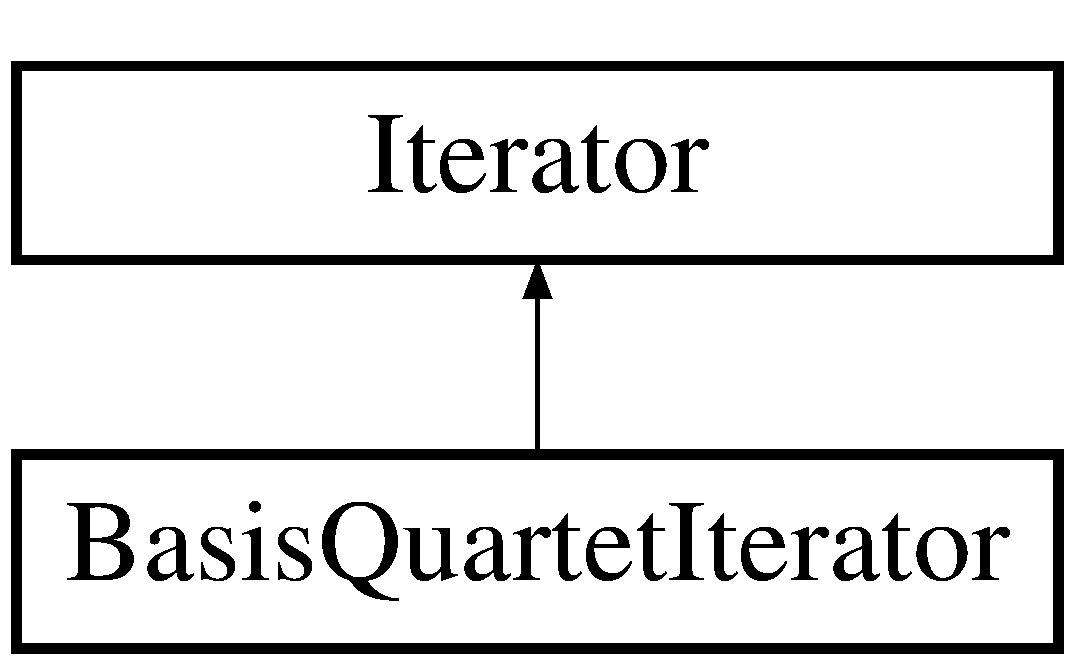
\includegraphics[height=2cm]{classJKBuilder_1_1BasisQuartetIterator}
\end{center}
\end{figure}
\subsection*{Public Member Functions}
\begin{DoxyCompactItemize}
\item 
\hyperlink{classJKBuilder_1_1BasisQuartetIterator_afac9e1e5415c1d0b7359faa353f6b86d}{BasisQuartetIterator} (const std::vector$<$ \hyperlink{classJKBuilder_1_1Shell}{Shell} $\ast$ $>$ \&ABS, bool start)
\item 
virtual void \hyperlink{classJKBuilder_1_1Iterator_a34ca36a99b20ae3170babadaffe51ed2}{Start} (int n=0)
\begin{DoxyCompactList}\small\item\em Returns an iterator suitable for starting on iteration n. \item\end{DoxyCompactList}\item 
virtual void \hyperlink{classJKBuilder_1_1Iterator_a5f692b73d2e160450f4617bb75825e11}{End} (int n=-\/1)
\begin{DoxyCompactList}\small\item\em Returns an iterator representing the state of the iterator after n iterations have occured. \item\end{DoxyCompactList}\item 
\hyperlink{classJKBuilder_1_1Iterator}{Iterator} \hyperlink{classJKBuilder_1_1Iterator_ac1702aedba13b4112b891b58dfd78eba}{operator++} (int)
\begin{DoxyCompactList}\small\item\em Increments the iterator after returning it's value. \item\end{DoxyCompactList}\item 
\hyperlink{classJKBuilder_1_1Iterator}{Iterator} \& \hyperlink{classJKBuilder_1_1Iterator_ae1f21c74128a5ef5d1b9de72ceb09be8}{operator++} ()
\begin{DoxyCompactList}\small\item\em Increments the iterator before returning it's value. \item\end{DoxyCompactList}\item 
bool \hyperlink{classJKBuilder_1_1Iterator_a1ea001976a5bc8ae8dc365e2a912b59a}{operator==} (const \hyperlink{classJKBuilder_1_1Iterator}{Iterator} \&other) const 
\item 
bool \hyperlink{classJKBuilder_1_1Iterator_a8c06af8ae0d9d1614ae9f81629275926}{operator!=} (const \hyperlink{classJKBuilder_1_1Iterator}{Iterator} \&other)
\begin{DoxyCompactList}\small\item\em Returns the opposite of operator==. \item\end{DoxyCompactList}\item 
void \hyperlink{classJKBuilder_1_1Iterator_aa83de505e29125c1d3ac7bb1b13ca15a}{SetStart} (std::vector$<$ int $>$ const \&other)
\begin{DoxyCompactList}\small\item\em Sets the N Indices to the N given in other. \item\end{DoxyCompactList}\item 
void \hyperlink{classJKBuilder_1_1Iterator_aad84ec668b5f41210db34c540aaa31fc}{SetEnd} (std::vector$<$ int $>$ const \&other)
\begin{DoxyCompactList}\small\item\em Sets the N MaxInd in other. \item\end{DoxyCompactList}\item 
int \hyperlink{classJKBuilder_1_1Iterator_a74247cf730a06b23fcb1ec64e5596b25}{operator\mbox{[}$\,$\mbox{]}} (const int i) const 
\begin{DoxyCompactList}\small\item\em Returns index i. \item\end{DoxyCompactList}\end{DoxyCompactItemize}
\subsection*{Protected Member Functions}
\begin{DoxyCompactItemize}
\item 
virtual void \hyperlink{classJKBuilder_1_1Iterator_a7874a07e98b52f4f147cde6f39353bae}{Iterate} ()
\end{DoxyCompactItemize}
\subsection*{Protected Attributes}
\begin{DoxyCompactItemize}
\item 
std::vector$<$ int $>$ \hyperlink{classJKBuilder_1_1Iterator_a20ca24f6d827aba144bb087c4bcb74a0}{CurrentValue}
\begin{DoxyCompactList}\small\item\em The current value. \item\end{DoxyCompactList}\item 
std::vector$<$ int $>$ \hyperlink{classJKBuilder_1_1Iterator_ab6b56d3c4e9353bc938dd6249cde9ca0}{MaxInd}
\begin{DoxyCompactList}\small\item\em This is a vector of length N containing the maximum each index can be. \item\end{DoxyCompactList}\end{DoxyCompactItemize}


\subsection{Detailed Description}
Iterates over the BasisPairs. 

\subsection{Constructor \& Destructor Documentation}
\hypertarget{classJKBuilder_1_1BasisQuartetIterator_afac9e1e5415c1d0b7359faa353f6b86d}{
\index{JKBuilder::BasisQuartetIterator@{JKBuilder::BasisQuartetIterator}!BasisQuartetIterator@{BasisQuartetIterator}}
\index{BasisQuartetIterator@{BasisQuartetIterator}!JKBuilder::BasisQuartetIterator@{JKBuilder::BasisQuartetIterator}}
\subsubsection[{BasisQuartetIterator}]{\setlength{\rightskip}{0pt plus 5cm}{\bf BasisQuartetIterator} (const std::vector$<$ {\bf Shell} $\ast$ $>$ \& {\em ABS}, \/  bool {\em start})}}
\label{classJKBuilder_1_1BasisQuartetIterator_afac9e1e5415c1d0b7359faa353f6b86d}


\subsection{Member Function Documentation}
\hypertarget{classJKBuilder_1_1Iterator_a7874a07e98b52f4f147cde6f39353bae}{
\index{JKBuilder::BasisQuartetIterator@{JKBuilder::BasisQuartetIterator}!Iterate@{Iterate}}
\index{Iterate@{Iterate}!JKBuilder::BasisQuartetIterator@{JKBuilder::BasisQuartetIterator}}
\subsubsection[{Iterate}]{\setlength{\rightskip}{0pt plus 5cm}void Iterate ()\hspace{0.3cm}{\ttfamily  \mbox{[}protected, virtual, inherited\mbox{]}}}}
\label{classJKBuilder_1_1Iterator_a7874a07e98b52f4f147cde6f39353bae}


Reimplemented in \hyperlink{classJKBuilder_1_1PairIterator_a7874a07e98b52f4f147cde6f39353bae}{PairIterator}, \hyperlink{classJKBuilder_1_1QuartetIterator_a7874a07e98b52f4f147cde6f39353bae}{QuartetIterator}, \hyperlink{classJKBuilder_1_1ShellPairIterator_a7874a07e98b52f4f147cde6f39353bae}{ShellPairIterator}, and \hyperlink{classJKBuilder_1_1SymmMatItr_a7874a07e98b52f4f147cde6f39353bae}{SymmMatItr}.\hypertarget{classJKBuilder_1_1Iterator_a34ca36a99b20ae3170babadaffe51ed2}{
\index{JKBuilder::BasisQuartetIterator@{JKBuilder::BasisQuartetIterator}!Start@{Start}}
\index{Start@{Start}!JKBuilder::BasisQuartetIterator@{JKBuilder::BasisQuartetIterator}}
\subsubsection[{Start}]{\setlength{\rightskip}{0pt plus 5cm}void Start (int {\em n} = {\ttfamily 0})\hspace{0.3cm}{\ttfamily  \mbox{[}virtual, inherited\mbox{]}}}}
\label{classJKBuilder_1_1Iterator_a34ca36a99b20ae3170babadaffe51ed2}


Returns an iterator suitable for starting on iteration n. 

Reimplemented in \hyperlink{classJKBuilder_1_1QuartetIterator_a34ca36a99b20ae3170babadaffe51ed2}{QuartetIterator}.\hypertarget{classJKBuilder_1_1Iterator_a5f692b73d2e160450f4617bb75825e11}{
\index{JKBuilder::BasisQuartetIterator@{JKBuilder::BasisQuartetIterator}!End@{End}}
\index{End@{End}!JKBuilder::BasisQuartetIterator@{JKBuilder::BasisQuartetIterator}}
\subsubsection[{End}]{\setlength{\rightskip}{0pt plus 5cm}void End (int {\em n} = {\ttfamily -\/1})\hspace{0.3cm}{\ttfamily  \mbox{[}virtual, inherited\mbox{]}}}}
\label{classJKBuilder_1_1Iterator_a5f692b73d2e160450f4617bb75825e11}


Returns an iterator representing the state of the iterator after n iterations have occured. The default argument is n=-\/1, which is a flag corresponding to the last iteration of the iterator 

Reimplemented in \hyperlink{classJKBuilder_1_1QuartetIterator_a5f692b73d2e160450f4617bb75825e11}{QuartetIterator}.\hypertarget{classJKBuilder_1_1Iterator_ac1702aedba13b4112b891b58dfd78eba}{
\index{JKBuilder::BasisQuartetIterator@{JKBuilder::BasisQuartetIterator}!operator++@{operator++}}
\index{operator++@{operator++}!JKBuilder::BasisQuartetIterator@{JKBuilder::BasisQuartetIterator}}
\subsubsection[{operator++}]{\setlength{\rightskip}{0pt plus 5cm}{\bf Iterator} operator++ (int)\hspace{0.3cm}{\ttfamily  \mbox{[}inherited\mbox{]}}}}
\label{classJKBuilder_1_1Iterator_ac1702aedba13b4112b891b58dfd78eba}


Increments the iterator after returning it's value. \hypertarget{classJKBuilder_1_1Iterator_ae1f21c74128a5ef5d1b9de72ceb09be8}{
\index{JKBuilder::BasisQuartetIterator@{JKBuilder::BasisQuartetIterator}!operator++@{operator++}}
\index{operator++@{operator++}!JKBuilder::BasisQuartetIterator@{JKBuilder::BasisQuartetIterator}}
\subsubsection[{operator++}]{\setlength{\rightskip}{0pt plus 5cm}{\bf Iterator} \& operator++ ()\hspace{0.3cm}{\ttfamily  \mbox{[}inherited\mbox{]}}}}
\label{classJKBuilder_1_1Iterator_ae1f21c74128a5ef5d1b9de72ceb09be8}


Increments the iterator before returning it's value. \hypertarget{classJKBuilder_1_1Iterator_a1ea001976a5bc8ae8dc365e2a912b59a}{
\index{JKBuilder::BasisQuartetIterator@{JKBuilder::BasisQuartetIterator}!operator==@{operator==}}
\index{operator==@{operator==}!JKBuilder::BasisQuartetIterator@{JKBuilder::BasisQuartetIterator}}
\subsubsection[{operator==}]{\setlength{\rightskip}{0pt plus 5cm}bool operator== (const {\bf Iterator} \& {\em other}) const\hspace{0.3cm}{\ttfamily  \mbox{[}inherited\mbox{]}}}}
\label{classJKBuilder_1_1Iterator_a1ea001976a5bc8ae8dc365e2a912b59a}


Reimplemented in \hyperlink{classJKBuilder_1_1PairIterator_a6b4e430066f478e5e400edd39ef93968}{PairIterator}.\hypertarget{classJKBuilder_1_1Iterator_a8c06af8ae0d9d1614ae9f81629275926}{
\index{JKBuilder::BasisQuartetIterator@{JKBuilder::BasisQuartetIterator}!operator!=@{operator!=}}
\index{operator!=@{operator!=}!JKBuilder::BasisQuartetIterator@{JKBuilder::BasisQuartetIterator}}
\subsubsection[{operator!=}]{\setlength{\rightskip}{0pt plus 5cm}bool operator!= (const {\bf Iterator} \& {\em other})\hspace{0.3cm}{\ttfamily  \mbox{[}inherited\mbox{]}}}}
\label{classJKBuilder_1_1Iterator_a8c06af8ae0d9d1614ae9f81629275926}


Returns the opposite of operator==. \hypertarget{classJKBuilder_1_1Iterator_aa83de505e29125c1d3ac7bb1b13ca15a}{
\index{JKBuilder::BasisQuartetIterator@{JKBuilder::BasisQuartetIterator}!SetStart@{SetStart}}
\index{SetStart@{SetStart}!JKBuilder::BasisQuartetIterator@{JKBuilder::BasisQuartetIterator}}
\subsubsection[{SetStart}]{\setlength{\rightskip}{0pt plus 5cm}void SetStart (std::vector$<$ int $>$ const \& {\em other})\hspace{0.3cm}{\ttfamily  \mbox{[}inherited\mbox{]}}}}
\label{classJKBuilder_1_1Iterator_aa83de505e29125c1d3ac7bb1b13ca15a}


Sets the N Indices to the N given in other. \hypertarget{classJKBuilder_1_1Iterator_aad84ec668b5f41210db34c540aaa31fc}{
\index{JKBuilder::BasisQuartetIterator@{JKBuilder::BasisQuartetIterator}!SetEnd@{SetEnd}}
\index{SetEnd@{SetEnd}!JKBuilder::BasisQuartetIterator@{JKBuilder::BasisQuartetIterator}}
\subsubsection[{SetEnd}]{\setlength{\rightskip}{0pt plus 5cm}void SetEnd (std::vector$<$ int $>$ const \& {\em other})\hspace{0.3cm}{\ttfamily  \mbox{[}inherited\mbox{]}}}}
\label{classJKBuilder_1_1Iterator_aad84ec668b5f41210db34c540aaa31fc}


Sets the N MaxInd in other. \hypertarget{classJKBuilder_1_1Iterator_a74247cf730a06b23fcb1ec64e5596b25}{
\index{JKBuilder::BasisQuartetIterator@{JKBuilder::BasisQuartetIterator}!operator\mbox{[}\mbox{]}@{operator[]}}
\index{operator\mbox{[}\mbox{]}@{operator[]}!JKBuilder::BasisQuartetIterator@{JKBuilder::BasisQuartetIterator}}
\subsubsection[{operator[]}]{\setlength{\rightskip}{0pt plus 5cm}int operator\mbox{[}$\,$\mbox{]} (const int {\em i}) const\hspace{0.3cm}{\ttfamily  \mbox{[}inherited\mbox{]}}}}
\label{classJKBuilder_1_1Iterator_a74247cf730a06b23fcb1ec64e5596b25}


Returns index i. 

\subsection{Member Data Documentation}
\hypertarget{classJKBuilder_1_1Iterator_a20ca24f6d827aba144bb087c4bcb74a0}{
\index{JKBuilder::BasisQuartetIterator@{JKBuilder::BasisQuartetIterator}!CurrentValue@{CurrentValue}}
\index{CurrentValue@{CurrentValue}!JKBuilder::BasisQuartetIterator@{JKBuilder::BasisQuartetIterator}}
\subsubsection[{CurrentValue}]{\setlength{\rightskip}{0pt plus 5cm}std::vector$<$int$>$ {\bf CurrentValue}\hspace{0.3cm}{\ttfamily  \mbox{[}protected, inherited\mbox{]}}}}
\label{classJKBuilder_1_1Iterator_a20ca24f6d827aba144bb087c4bcb74a0}


The current value. \hypertarget{classJKBuilder_1_1Iterator_ab6b56d3c4e9353bc938dd6249cde9ca0}{
\index{JKBuilder::BasisQuartetIterator@{JKBuilder::BasisQuartetIterator}!MaxInd@{MaxInd}}
\index{MaxInd@{MaxInd}!JKBuilder::BasisQuartetIterator@{JKBuilder::BasisQuartetIterator}}
\subsubsection[{MaxInd}]{\setlength{\rightskip}{0pt plus 5cm}std::vector$<$int$>$ {\bf MaxInd}\hspace{0.3cm}{\ttfamily  \mbox{[}protected, inherited\mbox{]}}}}
\label{classJKBuilder_1_1Iterator_ab6b56d3c4e9353bc938dd6249cde9ca0}


This is a vector of length N containing the maximum each index can be. 

The documentation for this class was generated from the following files:\begin{DoxyCompactItemize}
\item 
src/\hyperlink{Iterators_8h}{Iterators.h}\item 
src/\hyperlink{Iterator_8cpp}{Iterator.cpp}\end{DoxyCompactItemize}

\hypertarget{classJKBuilder_1_1BasisSet}{
\section{BasisSet Class Reference}
\label{classJKBuilder_1_1BasisSet}\index{JKBuilder::BasisSet@{JKBuilder::BasisSet}}
}


An abstract base class for Gaussian basis sets.  


{\ttfamily \#include $<$BasisSet.h$>$}Inheritance diagram for BasisSet::\begin{figure}[H]
\begin{center}
\leavevmode
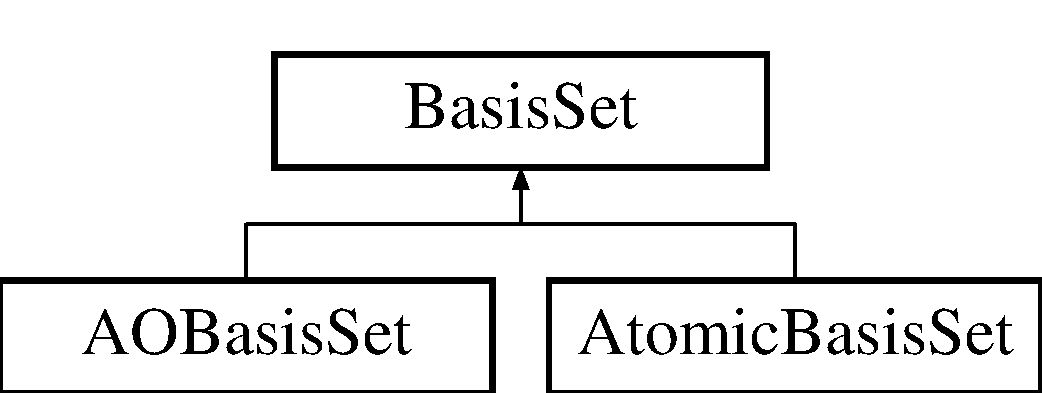
\includegraphics[height=2cm]{classJKBuilder_1_1BasisSet}
\end{center}
\end{figure}
\subsection*{Public Member Functions}
\begin{DoxyCompactItemize}
\item 
\hyperlink{classJKBuilder_1_1BasisSet_a902600fb65d5c4d7f7041316b1845b07}{BasisSet} ()
\begin{DoxyCompactList}\small\item\em Sets everything to 0. \item\end{DoxyCompactList}\item 
virtual \hyperlink{classJKBuilder_1_1BasisSet_acd6bebfe86051930ab0931d7d2486cce}{$\sim$BasisSet} ()
\begin{DoxyCompactList}\small\item\em No memory allocated=nothing done. \item\end{DoxyCompactList}\item 
virtual int \hyperlink{classJKBuilder_1_1BasisSet_a0eb3b46d258dffcfbc3e4db91f60f4f8}{GetNShells} ()=0
\begin{DoxyCompactList}\small\item\em Returns the number of shells in this basis set. \item\end{DoxyCompactList}\item 
virtual int \hyperlink{classJKBuilder_1_1BasisSet_a1167cdb6f1e1ba08ba6cbffa0b32ca77}{GetNBasis} ()=0
\begin{DoxyCompactList}\small\item\em Returns the number of basis functions. \item\end{DoxyCompactList}\item 
virtual int \hyperlink{classJKBuilder_1_1BasisSet_a5580c8eff6cb4242a298c15da2292fa4}{GetMaxL} ()=0
\begin{DoxyCompactList}\small\item\em Returns the maximum momentum. \item\end{DoxyCompactList}\item 
virtual int \hyperlink{classJKBuilder_1_1BasisSet_a4e5f8295f4fe1ecf1a910ae2fcb46c1f}{GetMaxPrim} (int \&ID)=0
\begin{DoxyCompactList}\small\item\em Returns the maximum number of primitives and the ID of the shell with that number. \item\end{DoxyCompactList}\item 
virtual int \hyperlink{classJKBuilder_1_1BasisSet_a7c12871050e478f6a22c4c1c46bd4b21}{GetMaxBasis} ()=0
\begin{DoxyCompactList}\small\item\em Returns the maximum number of basis functions in this basis set;. \item\end{DoxyCompactList}\item 
virtual void \hyperlink{classJKBuilder_1_1BasisSet_a388f572c62279f839ee138a9afbdeeb5}{print} ()
\begin{DoxyCompactList}\small\item\em Prints the basis set. \item\end{DoxyCompactList}\item 
virtual int \hyperlink{classJKBuilder_1_1BasisSet_abc886cd4e35d3c56a0250b7d06986f61}{GetNPrims} ()
\begin{DoxyCompactList}\small\item\em Returns the number of primitives. \item\end{DoxyCompactList}\end{DoxyCompactItemize}
\subsection*{Protected Attributes}
\begin{DoxyCompactItemize}
\item 
int \hyperlink{classJKBuilder_1_1BasisSet_a41e2bc1e52da2859eabe6586e4451663}{NBasis}
\begin{DoxyCompactList}\small\item\em The number of basis functions in this basis. \item\end{DoxyCompactList}\item 
int \hyperlink{classJKBuilder_1_1BasisSet_a9f13901f058284051a35aabd9d69c6d5}{NShells}
\begin{DoxyCompactList}\small\item\em The number of shells in this basis set. \item\end{DoxyCompactList}\item 
int \hyperlink{classJKBuilder_1_1BasisSet_ad30990632a28f27018d2b497e263caf1}{NPrims}
\begin{DoxyCompactList}\small\item\em The number of primitives in this basis set. \item\end{DoxyCompactList}\item 
int \hyperlink{classJKBuilder_1_1BasisSet_a8fce14d0246c865eea79bf2869b02997}{max\_\-momentum}
\begin{DoxyCompactList}\small\item\em The maximum momentum. \item\end{DoxyCompactList}\item 
int \hyperlink{classJKBuilder_1_1BasisSet_aeb188680b23f4d32ea9a65468e5ba71d}{max\_\-prims}
\begin{DoxyCompactList}\small\item\em The maximum number of primitives. \item\end{DoxyCompactList}\item 
int \hyperlink{classJKBuilder_1_1BasisSet_acdabb925780e7292114dfa2ace8b9d8e}{max\_\-prims\_\-ID}
\begin{DoxyCompactList}\small\item\em The ID of the shell with the maximum number of primitives,counting from 0. \item\end{DoxyCompactList}\item 
int \hyperlink{classJKBuilder_1_1BasisSet_af29e85e56ea63952fc7a1ede8d10426f}{max\_\-basis}
\begin{DoxyCompactList}\small\item\em The maximum number of basis functions in this basis. \item\end{DoxyCompactList}\end{DoxyCompactItemize}


\subsection{Detailed Description}
An abstract base class for Gaussian basis sets. The basis set for our system can be thought of as a collection of the basis sets for each \hyperlink{classJKBuilder_1_1atom}{atom}, each of which is a basis set in its own right. This class is intended to provide the common functionality for these two basis sets. 

\subsection{Constructor \& Destructor Documentation}
\hypertarget{classJKBuilder_1_1BasisSet_a902600fb65d5c4d7f7041316b1845b07}{
\index{JKBuilder::BasisSet@{JKBuilder::BasisSet}!BasisSet@{BasisSet}}
\index{BasisSet@{BasisSet}!JKBuilder::BasisSet@{JKBuilder::BasisSet}}
\subsubsection[{BasisSet}]{\setlength{\rightskip}{0pt plus 5cm}{\bf BasisSet} ()}}
\label{classJKBuilder_1_1BasisSet_a902600fb65d5c4d7f7041316b1845b07}


Sets everything to 0. \hypertarget{classJKBuilder_1_1BasisSet_acd6bebfe86051930ab0931d7d2486cce}{
\index{JKBuilder::BasisSet@{JKBuilder::BasisSet}!$\sim$BasisSet@{$\sim$BasisSet}}
\index{$\sim$BasisSet@{$\sim$BasisSet}!JKBuilder::BasisSet@{JKBuilder::BasisSet}}
\subsubsection[{$\sim$BasisSet}]{\setlength{\rightskip}{0pt plus 5cm}$\sim${\bf BasisSet} ()\hspace{0.3cm}{\ttfamily  \mbox{[}virtual\mbox{]}}}}
\label{classJKBuilder_1_1BasisSet_acd6bebfe86051930ab0931d7d2486cce}


No memory allocated=nothing done. 

\subsection{Member Function Documentation}
\hypertarget{classJKBuilder_1_1BasisSet_a0eb3b46d258dffcfbc3e4db91f60f4f8}{
\index{JKBuilder::BasisSet@{JKBuilder::BasisSet}!GetNShells@{GetNShells}}
\index{GetNShells@{GetNShells}!JKBuilder::BasisSet@{JKBuilder::BasisSet}}
\subsubsection[{GetNShells}]{\setlength{\rightskip}{0pt plus 5cm}virtual int GetNShells ()\hspace{0.3cm}{\ttfamily  \mbox{[}pure virtual\mbox{]}}}}
\label{classJKBuilder_1_1BasisSet_a0eb3b46d258dffcfbc3e4db91f60f4f8}


Returns the number of shells in this basis set. 

Implemented in \hyperlink{classJKBuilder_1_1AtomicBasisSet_aa62be7e63d0f2b5828ab72cec3ce8590}{AtomicBasisSet}, and \hyperlink{classJKBuilder_1_1AOBasisSet_aa62be7e63d0f2b5828ab72cec3ce8590}{AOBasisSet}.\hypertarget{classJKBuilder_1_1BasisSet_a1167cdb6f1e1ba08ba6cbffa0b32ca77}{
\index{JKBuilder::BasisSet@{JKBuilder::BasisSet}!GetNBasis@{GetNBasis}}
\index{GetNBasis@{GetNBasis}!JKBuilder::BasisSet@{JKBuilder::BasisSet}}
\subsubsection[{GetNBasis}]{\setlength{\rightskip}{0pt plus 5cm}virtual int GetNBasis ()\hspace{0.3cm}{\ttfamily  \mbox{[}pure virtual\mbox{]}}}}
\label{classJKBuilder_1_1BasisSet_a1167cdb6f1e1ba08ba6cbffa0b32ca77}


Returns the number of basis functions. 

Implemented in \hyperlink{classJKBuilder_1_1AtomicBasisSet_a297c144fb990284ac5973c99cdd55f91}{AtomicBasisSet}, and \hyperlink{classJKBuilder_1_1AOBasisSet_a297c144fb990284ac5973c99cdd55f91}{AOBasisSet}.\hypertarget{classJKBuilder_1_1BasisSet_a5580c8eff6cb4242a298c15da2292fa4}{
\index{JKBuilder::BasisSet@{JKBuilder::BasisSet}!GetMaxL@{GetMaxL}}
\index{GetMaxL@{GetMaxL}!JKBuilder::BasisSet@{JKBuilder::BasisSet}}
\subsubsection[{GetMaxL}]{\setlength{\rightskip}{0pt plus 5cm}virtual int GetMaxL ()\hspace{0.3cm}{\ttfamily  \mbox{[}pure virtual\mbox{]}}}}
\label{classJKBuilder_1_1BasisSet_a5580c8eff6cb4242a298c15da2292fa4}


Returns the maximum momentum. 

Implemented in \hyperlink{classJKBuilder_1_1AtomicBasisSet_af6694a93cc5d86a8f3cd1aa984a0cdc3}{AtomicBasisSet}, and \hyperlink{classJKBuilder_1_1AOBasisSet_af6694a93cc5d86a8f3cd1aa984a0cdc3}{AOBasisSet}.\hypertarget{classJKBuilder_1_1BasisSet_a4e5f8295f4fe1ecf1a910ae2fcb46c1f}{
\index{JKBuilder::BasisSet@{JKBuilder::BasisSet}!GetMaxPrim@{GetMaxPrim}}
\index{GetMaxPrim@{GetMaxPrim}!JKBuilder::BasisSet@{JKBuilder::BasisSet}}
\subsubsection[{GetMaxPrim}]{\setlength{\rightskip}{0pt plus 5cm}virtual int GetMaxPrim (int \& {\em ID})\hspace{0.3cm}{\ttfamily  \mbox{[}pure virtual\mbox{]}}}}
\label{classJKBuilder_1_1BasisSet_a4e5f8295f4fe1ecf1a910ae2fcb46c1f}


Returns the maximum number of primitives and the ID of the shell with that number. 

Implemented in \hyperlink{classJKBuilder_1_1AtomicBasisSet_a03191bf41d6e3a2445dd3eb8640305be}{AtomicBasisSet}, and \hyperlink{classJKBuilder_1_1AOBasisSet_a03191bf41d6e3a2445dd3eb8640305be}{AOBasisSet}.\hypertarget{classJKBuilder_1_1BasisSet_a7c12871050e478f6a22c4c1c46bd4b21}{
\index{JKBuilder::BasisSet@{JKBuilder::BasisSet}!GetMaxBasis@{GetMaxBasis}}
\index{GetMaxBasis@{GetMaxBasis}!JKBuilder::BasisSet@{JKBuilder::BasisSet}}
\subsubsection[{GetMaxBasis}]{\setlength{\rightskip}{0pt plus 5cm}virtual int GetMaxBasis ()\hspace{0.3cm}{\ttfamily  \mbox{[}pure virtual\mbox{]}}}}
\label{classJKBuilder_1_1BasisSet_a7c12871050e478f6a22c4c1c46bd4b21}


Returns the maximum number of basis functions in this basis set;. 

Implemented in \hyperlink{classJKBuilder_1_1AtomicBasisSet_adcda37af511d6b4f8d305fcba2da5c4a}{AtomicBasisSet}, and \hyperlink{classJKBuilder_1_1AOBasisSet_adcda37af511d6b4f8d305fcba2da5c4a}{AOBasisSet}.\hypertarget{classJKBuilder_1_1BasisSet_a388f572c62279f839ee138a9afbdeeb5}{
\index{JKBuilder::BasisSet@{JKBuilder::BasisSet}!print@{print}}
\index{print@{print}!JKBuilder::BasisSet@{JKBuilder::BasisSet}}
\subsubsection[{print}]{\setlength{\rightskip}{0pt plus 5cm}void print ()\hspace{0.3cm}{\ttfamily  \mbox{[}virtual\mbox{]}}}}
\label{classJKBuilder_1_1BasisSet_a388f572c62279f839ee138a9afbdeeb5}


Prints the basis set. 

Reimplemented in \hyperlink{classJKBuilder_1_1AtomicBasisSet_a388f572c62279f839ee138a9afbdeeb5}{AtomicBasisSet}, and \hyperlink{classJKBuilder_1_1AOBasisSet_a388f572c62279f839ee138a9afbdeeb5}{AOBasisSet}.\hypertarget{classJKBuilder_1_1BasisSet_abc886cd4e35d3c56a0250b7d06986f61}{
\index{JKBuilder::BasisSet@{JKBuilder::BasisSet}!GetNPrims@{GetNPrims}}
\index{GetNPrims@{GetNPrims}!JKBuilder::BasisSet@{JKBuilder::BasisSet}}
\subsubsection[{GetNPrims}]{\setlength{\rightskip}{0pt plus 5cm}int GetNPrims ()\hspace{0.3cm}{\ttfamily  \mbox{[}virtual\mbox{]}}}}
\label{classJKBuilder_1_1BasisSet_abc886cd4e35d3c56a0250b7d06986f61}


Returns the number of primitives. 

\subsection{Member Data Documentation}
\hypertarget{classJKBuilder_1_1BasisSet_a41e2bc1e52da2859eabe6586e4451663}{
\index{JKBuilder::BasisSet@{JKBuilder::BasisSet}!NBasis@{NBasis}}
\index{NBasis@{NBasis}!JKBuilder::BasisSet@{JKBuilder::BasisSet}}
\subsubsection[{NBasis}]{\setlength{\rightskip}{0pt plus 5cm}int {\bf NBasis}\hspace{0.3cm}{\ttfamily  \mbox{[}protected\mbox{]}}}}
\label{classJKBuilder_1_1BasisSet_a41e2bc1e52da2859eabe6586e4451663}


The number of basis functions in this basis. \hypertarget{classJKBuilder_1_1BasisSet_a9f13901f058284051a35aabd9d69c6d5}{
\index{JKBuilder::BasisSet@{JKBuilder::BasisSet}!NShells@{NShells}}
\index{NShells@{NShells}!JKBuilder::BasisSet@{JKBuilder::BasisSet}}
\subsubsection[{NShells}]{\setlength{\rightskip}{0pt plus 5cm}int {\bf NShells}\hspace{0.3cm}{\ttfamily  \mbox{[}protected\mbox{]}}}}
\label{classJKBuilder_1_1BasisSet_a9f13901f058284051a35aabd9d69c6d5}


The number of shells in this basis set. \hypertarget{classJKBuilder_1_1BasisSet_ad30990632a28f27018d2b497e263caf1}{
\index{JKBuilder::BasisSet@{JKBuilder::BasisSet}!NPrims@{NPrims}}
\index{NPrims@{NPrims}!JKBuilder::BasisSet@{JKBuilder::BasisSet}}
\subsubsection[{NPrims}]{\setlength{\rightskip}{0pt plus 5cm}int {\bf NPrims}\hspace{0.3cm}{\ttfamily  \mbox{[}protected\mbox{]}}}}
\label{classJKBuilder_1_1BasisSet_ad30990632a28f27018d2b497e263caf1}


The number of primitives in this basis set. \hypertarget{classJKBuilder_1_1BasisSet_a8fce14d0246c865eea79bf2869b02997}{
\index{JKBuilder::BasisSet@{JKBuilder::BasisSet}!max\_\-momentum@{max\_\-momentum}}
\index{max\_\-momentum@{max\_\-momentum}!JKBuilder::BasisSet@{JKBuilder::BasisSet}}
\subsubsection[{max\_\-momentum}]{\setlength{\rightskip}{0pt plus 5cm}int {\bf max\_\-momentum}\hspace{0.3cm}{\ttfamily  \mbox{[}protected\mbox{]}}}}
\label{classJKBuilder_1_1BasisSet_a8fce14d0246c865eea79bf2869b02997}


The maximum momentum. \hypertarget{classJKBuilder_1_1BasisSet_aeb188680b23f4d32ea9a65468e5ba71d}{
\index{JKBuilder::BasisSet@{JKBuilder::BasisSet}!max\_\-prims@{max\_\-prims}}
\index{max\_\-prims@{max\_\-prims}!JKBuilder::BasisSet@{JKBuilder::BasisSet}}
\subsubsection[{max\_\-prims}]{\setlength{\rightskip}{0pt plus 5cm}int {\bf max\_\-prims}\hspace{0.3cm}{\ttfamily  \mbox{[}protected\mbox{]}}}}
\label{classJKBuilder_1_1BasisSet_aeb188680b23f4d32ea9a65468e5ba71d}


The maximum number of primitives. \hypertarget{classJKBuilder_1_1BasisSet_acdabb925780e7292114dfa2ace8b9d8e}{
\index{JKBuilder::BasisSet@{JKBuilder::BasisSet}!max\_\-prims\_\-ID@{max\_\-prims\_\-ID}}
\index{max\_\-prims\_\-ID@{max\_\-prims\_\-ID}!JKBuilder::BasisSet@{JKBuilder::BasisSet}}
\subsubsection[{max\_\-prims\_\-ID}]{\setlength{\rightskip}{0pt plus 5cm}int {\bf max\_\-prims\_\-ID}\hspace{0.3cm}{\ttfamily  \mbox{[}protected\mbox{]}}}}
\label{classJKBuilder_1_1BasisSet_acdabb925780e7292114dfa2ace8b9d8e}


The ID of the shell with the maximum number of primitives,counting from 0. \hypertarget{classJKBuilder_1_1BasisSet_af29e85e56ea63952fc7a1ede8d10426f}{
\index{JKBuilder::BasisSet@{JKBuilder::BasisSet}!max\_\-basis@{max\_\-basis}}
\index{max\_\-basis@{max\_\-basis}!JKBuilder::BasisSet@{JKBuilder::BasisSet}}
\subsubsection[{max\_\-basis}]{\setlength{\rightskip}{0pt plus 5cm}int {\bf max\_\-basis}\hspace{0.3cm}{\ttfamily  \mbox{[}protected\mbox{]}}}}
\label{classJKBuilder_1_1BasisSet_af29e85e56ea63952fc7a1ede8d10426f}


The maximum number of basis functions in this basis. 

The documentation for this class was generated from the following files:\begin{DoxyCompactItemize}
\item 
src/\hyperlink{BasisSet_8h}{BasisSet.h}\item 
src/\hyperlink{BasisSet_8cpp}{BasisSet.cpp}\end{DoxyCompactItemize}

\hypertarget{classJKBuilder_1_1CartShell}{
\section{CartShell Class Reference}
\label{classJKBuilder_1_1CartShell}\index{JKBuilder::CartShell@{JKBuilder::CartShell}}
}


Specialization of \hyperlink{classJKBuilder_1_1Shell}{Shell} to Cartesian Gaussians.  


{\ttfamily \#include $<$BasisSet.h$>$}Inheritance diagram for CartShell::\begin{figure}[H]
\begin{center}
\leavevmode
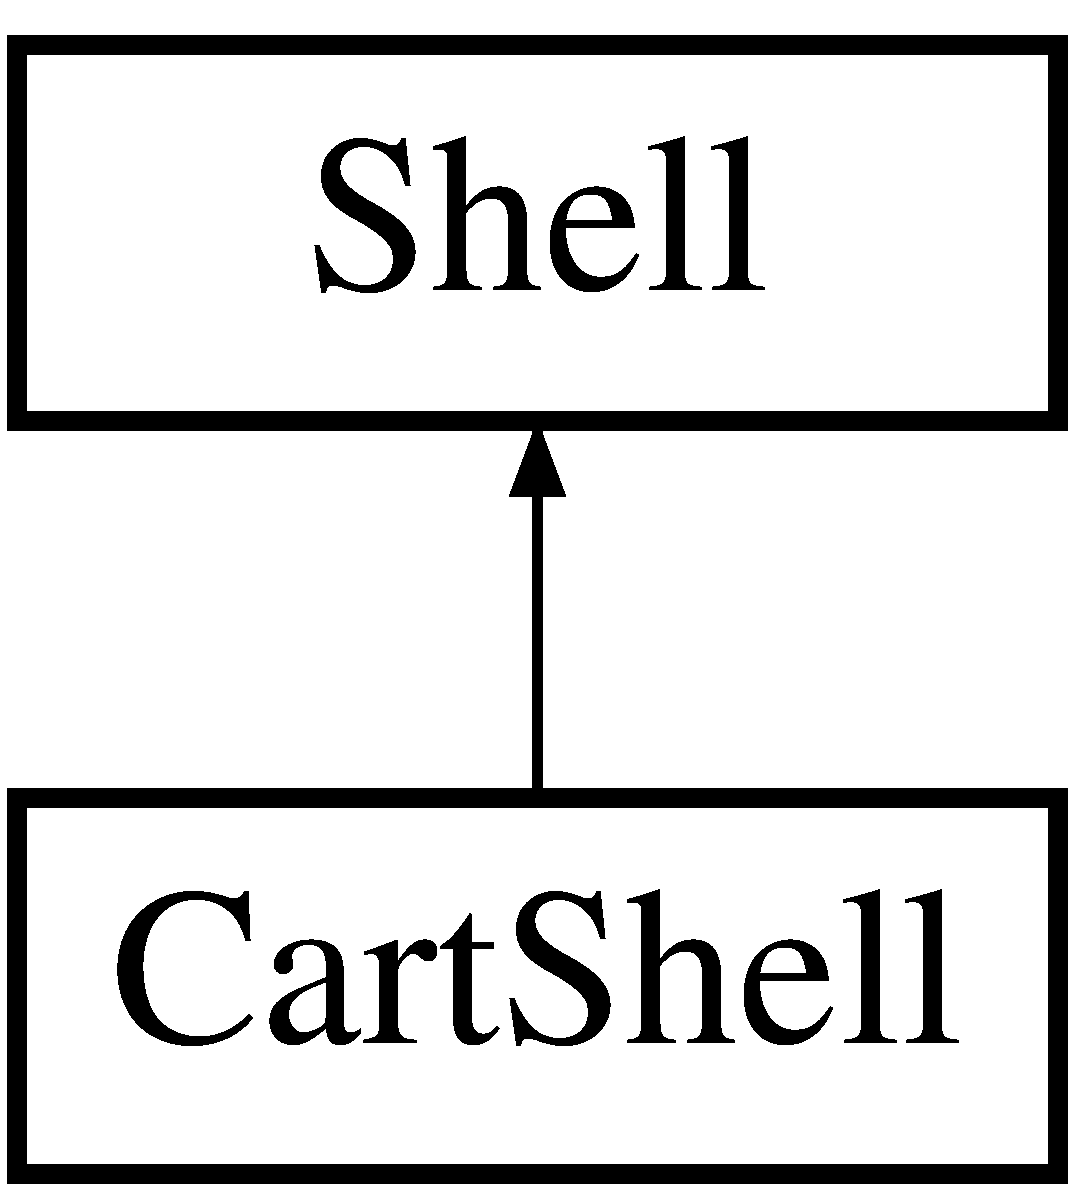
\includegraphics[height=2cm]{classJKBuilder_1_1CartShell}
\end{center}
\end{figure}
\subsection*{Public Member Functions}
\begin{DoxyCompactItemize}
\item 
\hyperlink{classJKBuilder_1_1CartShell_a57fcc9d47cb98edd56f6e2122f15afd6}{CartShell} (int \hyperlink{classJKBuilder_1_1Shell_a89606eca6b563ec68d2da2e84657736f}{l}=0)
\begin{DoxyCompactList}\small\item\em Calls the \hyperlink{classJKBuilder_1_1Shell}{Shell} constructor with IsCart=true. \item\end{DoxyCompactList}\item 
int \hyperlink{classJKBuilder_1_1CartShell_a297c144fb990284ac5973c99cdd55f91}{GetNBasis} ()
\begin{DoxyCompactList}\small\item\em Returns the number of basis functions. \item\end{DoxyCompactList}\item 
int \hyperlink{classJKBuilder_1_1Shell_abc886cd4e35d3c56a0250b7d06986f61}{GetNPrims} ()
\begin{DoxyCompactList}\small\item\em Returns the number of primitives. \item\end{DoxyCompactList}\item 
int \hyperlink{classJKBuilder_1_1Shell_a7cc8fc5bc043267a7b47e69503e0e308}{GetL} ()
\begin{DoxyCompactList}\small\item\em Returns the angular momentum. \item\end{DoxyCompactList}\item 
bool \hyperlink{classJKBuilder_1_1Shell_a75c22d97e837f5c439eb51aa223bed98}{IsCart} ()
\begin{DoxyCompactList}\small\item\em Returns true if this a Cartesian like shell. \item\end{DoxyCompactList}\item 
void \hyperlink{classJKBuilder_1_1Shell_a20ec923cb07d5d3762fffa4501d09924}{AddPrimitive} (double c0, double beta0)
\begin{DoxyCompactList}\small\item\em Creates a primitive with expansion coefficient c0 and exponent scale factor beta0. \item\end{DoxyCompactList}\item 
\hyperlink{classJKBuilder_1_1Primitive}{Primitive} $\ast$ \hyperlink{classJKBuilder_1_1Shell_ae98a68bcb237e53c8c063aded1b34f2e}{operator\mbox{[}$\,$\mbox{]}} (const int i)
\begin{DoxyCompactList}\small\item\em Returns a pointer to the i-\/th primitive. \item\end{DoxyCompactList}\item 
void \hyperlink{classJKBuilder_1_1Shell_a388f572c62279f839ee138a9afbdeeb5}{print} ()
\begin{DoxyCompactList}\small\item\em Prints out the shell. \item\end{DoxyCompactList}\end{DoxyCompactItemize}
\subsection*{Protected Attributes}
\begin{DoxyCompactItemize}
\item 
bool \hyperlink{classJKBuilder_1_1Shell_a8a5f217a40aac0ce092effdd9b6db9f6}{spherical}
\begin{DoxyCompactList}\small\item\em True if spherical, false if Cartesian. \item\end{DoxyCompactList}\item 
int \hyperlink{classJKBuilder_1_1Shell_a89606eca6b563ec68d2da2e84657736f}{l}
\begin{DoxyCompactList}\small\item\em The angular momentum of this shell. \item\end{DoxyCompactList}\item 
std::vector$<$ \hyperlink{classJKBuilder_1_1Primitive}{Primitive} $\ast$ $>$ \hyperlink{classJKBuilder_1_1Shell_afd0049f3a997082e636f4dae72879da2}{gi}
\begin{DoxyCompactList}\small\item\em A vector of the Primitives for this shell. \item\end{DoxyCompactList}\end{DoxyCompactItemize}


\subsection{Detailed Description}
Specialization of \hyperlink{classJKBuilder_1_1Shell}{Shell} to Cartesian Gaussians. In a Cartesian Gaussian of angular momentum $\ell=a+b+c$, we can assign quantum numbers between 0 and $\ell$ to each of the three numbers; however, the value of the third is set once we have choosen the first two. This means we can only really choose two numbers from the possible set. If we let $a=\ell$ then $b=c=0$ necessarily. If we let $a=\ell-1$ then $\lbrace b=1,c=0\rbrace$ or $\lbrace b=0,c=1\rbrace$. It is now apparent that in general if $a=\ell-\theta$, then we have $\theta+1$ choices of pairs of $b$ and $c$, which correspond to the choices for b, which are each value between 0 and $\theta$. This means:

\begin{eqnarray*} \rm{NBasis}=&\sum_{i=0}^\ell\left(i+1\right)\\ =&(\ell+1)+\sum_{i=1}^\ell i\\ =&(\ell+1)+\frac{\ell\left(\ell+1\right)}{2}\\ =&\frac{2\ell+2+\ell^2+\ell}{2}\\ =&\frac{\left(\ell +1\right)\left(\ell +2\right)}{2} \end{eqnarray*} 

\subsection{Constructor \& Destructor Documentation}
\hypertarget{classJKBuilder_1_1CartShell_a57fcc9d47cb98edd56f6e2122f15afd6}{
\index{JKBuilder::CartShell@{JKBuilder::CartShell}!CartShell@{CartShell}}
\index{CartShell@{CartShell}!JKBuilder::CartShell@{JKBuilder::CartShell}}
\subsubsection[{CartShell}]{\setlength{\rightskip}{0pt plus 5cm}{\bf CartShell} (int {\em l} = {\ttfamily 0})}}
\label{classJKBuilder_1_1CartShell_a57fcc9d47cb98edd56f6e2122f15afd6}


Calls the \hyperlink{classJKBuilder_1_1Shell}{Shell} constructor with IsCart=true. 

\subsection{Member Function Documentation}
\hypertarget{classJKBuilder_1_1CartShell_a297c144fb990284ac5973c99cdd55f91}{
\index{JKBuilder::CartShell@{JKBuilder::CartShell}!GetNBasis@{GetNBasis}}
\index{GetNBasis@{GetNBasis}!JKBuilder::CartShell@{JKBuilder::CartShell}}
\subsubsection[{GetNBasis}]{\setlength{\rightskip}{0pt plus 5cm}int GetNBasis ()\hspace{0.3cm}{\ttfamily  \mbox{[}virtual\mbox{]}}}}
\label{classJKBuilder_1_1CartShell_a297c144fb990284ac5973c99cdd55f91}


Returns the number of basis functions. 

Implements \hyperlink{classJKBuilder_1_1Shell_a1167cdb6f1e1ba08ba6cbffa0b32ca77}{Shell}.\hypertarget{classJKBuilder_1_1Shell_abc886cd4e35d3c56a0250b7d06986f61}{
\index{JKBuilder::CartShell@{JKBuilder::CartShell}!GetNPrims@{GetNPrims}}
\index{GetNPrims@{GetNPrims}!JKBuilder::CartShell@{JKBuilder::CartShell}}
\subsubsection[{GetNPrims}]{\setlength{\rightskip}{0pt plus 5cm}int GetNPrims ()\hspace{0.3cm}{\ttfamily  \mbox{[}inherited\mbox{]}}}}
\label{classJKBuilder_1_1Shell_abc886cd4e35d3c56a0250b7d06986f61}


Returns the number of primitives. \hypertarget{classJKBuilder_1_1Shell_a7cc8fc5bc043267a7b47e69503e0e308}{
\index{JKBuilder::CartShell@{JKBuilder::CartShell}!GetL@{GetL}}
\index{GetL@{GetL}!JKBuilder::CartShell@{JKBuilder::CartShell}}
\subsubsection[{GetL}]{\setlength{\rightskip}{0pt plus 5cm}int GetL ()\hspace{0.3cm}{\ttfamily  \mbox{[}inherited\mbox{]}}}}
\label{classJKBuilder_1_1Shell_a7cc8fc5bc043267a7b47e69503e0e308}


Returns the angular momentum. \hypertarget{classJKBuilder_1_1Shell_a75c22d97e837f5c439eb51aa223bed98}{
\index{JKBuilder::CartShell@{JKBuilder::CartShell}!IsCart@{IsCart}}
\index{IsCart@{IsCart}!JKBuilder::CartShell@{JKBuilder::CartShell}}
\subsubsection[{IsCart}]{\setlength{\rightskip}{0pt plus 5cm}bool IsCart ()\hspace{0.3cm}{\ttfamily  \mbox{[}inherited\mbox{]}}}}
\label{classJKBuilder_1_1Shell_a75c22d97e837f5c439eb51aa223bed98}


Returns true if this a Cartesian like shell. \hypertarget{classJKBuilder_1_1Shell_a20ec923cb07d5d3762fffa4501d09924}{
\index{JKBuilder::CartShell@{JKBuilder::CartShell}!AddPrimitive@{AddPrimitive}}
\index{AddPrimitive@{AddPrimitive}!JKBuilder::CartShell@{JKBuilder::CartShell}}
\subsubsection[{AddPrimitive}]{\setlength{\rightskip}{0pt plus 5cm}void AddPrimitive (double {\em c0}, \/  double {\em beta0})\hspace{0.3cm}{\ttfamily  \mbox{[}inherited\mbox{]}}}}
\label{classJKBuilder_1_1Shell_a20ec923cb07d5d3762fffa4501d09924}


Creates a primitive with expansion coefficient c0 and exponent scale factor beta0. \hypertarget{classJKBuilder_1_1Shell_ae98a68bcb237e53c8c063aded1b34f2e}{
\index{JKBuilder::CartShell@{JKBuilder::CartShell}!operator\mbox{[}\mbox{]}@{operator[]}}
\index{operator\mbox{[}\mbox{]}@{operator[]}!JKBuilder::CartShell@{JKBuilder::CartShell}}
\subsubsection[{operator[]}]{\setlength{\rightskip}{0pt plus 5cm}{\bf Primitive} $\ast$ operator\mbox{[}$\,$\mbox{]} (const int {\em i})\hspace{0.3cm}{\ttfamily  \mbox{[}inherited\mbox{]}}}}
\label{classJKBuilder_1_1Shell_ae98a68bcb237e53c8c063aded1b34f2e}


Returns a pointer to the i-\/th primitive. \hypertarget{classJKBuilder_1_1Shell_a388f572c62279f839ee138a9afbdeeb5}{
\index{JKBuilder::CartShell@{JKBuilder::CartShell}!print@{print}}
\index{print@{print}!JKBuilder::CartShell@{JKBuilder::CartShell}}
\subsubsection[{print}]{\setlength{\rightskip}{0pt plus 5cm}void print ()\hspace{0.3cm}{\ttfamily  \mbox{[}inherited\mbox{]}}}}
\label{classJKBuilder_1_1Shell_a388f572c62279f839ee138a9afbdeeb5}


Prints out the shell. 

\subsection{Member Data Documentation}
\hypertarget{classJKBuilder_1_1Shell_a8a5f217a40aac0ce092effdd9b6db9f6}{
\index{JKBuilder::CartShell@{JKBuilder::CartShell}!spherical@{spherical}}
\index{spherical@{spherical}!JKBuilder::CartShell@{JKBuilder::CartShell}}
\subsubsection[{spherical}]{\setlength{\rightskip}{0pt plus 5cm}bool {\bf spherical}\hspace{0.3cm}{\ttfamily  \mbox{[}protected, inherited\mbox{]}}}}
\label{classJKBuilder_1_1Shell_a8a5f217a40aac0ce092effdd9b6db9f6}


True if spherical, false if Cartesian. \hypertarget{classJKBuilder_1_1Shell_a89606eca6b563ec68d2da2e84657736f}{
\index{JKBuilder::CartShell@{JKBuilder::CartShell}!l@{l}}
\index{l@{l}!JKBuilder::CartShell@{JKBuilder::CartShell}}
\subsubsection[{l}]{\setlength{\rightskip}{0pt plus 5cm}int {\bf l}\hspace{0.3cm}{\ttfamily  \mbox{[}protected, inherited\mbox{]}}}}
\label{classJKBuilder_1_1Shell_a89606eca6b563ec68d2da2e84657736f}


The angular momentum of this shell. \hypertarget{classJKBuilder_1_1Shell_afd0049f3a997082e636f4dae72879da2}{
\index{JKBuilder::CartShell@{JKBuilder::CartShell}!gi@{gi}}
\index{gi@{gi}!JKBuilder::CartShell@{JKBuilder::CartShell}}
\subsubsection[{gi}]{\setlength{\rightskip}{0pt plus 5cm}std::vector$<${\bf Primitive}$\ast$$>$ {\bf gi}\hspace{0.3cm}{\ttfamily  \mbox{[}protected, inherited\mbox{]}}}}
\label{classJKBuilder_1_1Shell_afd0049f3a997082e636f4dae72879da2}


A vector of the Primitives for this shell. 

The documentation for this class was generated from the following files:\begin{DoxyCompactItemize}
\item 
src/\hyperlink{BasisSet_8h}{BasisSet.h}\item 
src/\hyperlink{BasisSet_8cpp}{BasisSet.cpp}\end{DoxyCompactItemize}

\hypertarget{classJKBuilder_1_1CG2SG}{
\section{CG2SG Class Reference}
\label{classJKBuilder_1_1CG2SG}\index{JKBuilder::CG2SG@{JKBuilder::CG2SG}}
}


This class handles the transformation from Cartesian Gaussians to Spherical Gaussians.  


{\ttfamily \#include $<$CG2SG.h$>$}Inheritance diagram for CG2SG::\begin{figure}[H]
\begin{center}
\leavevmode
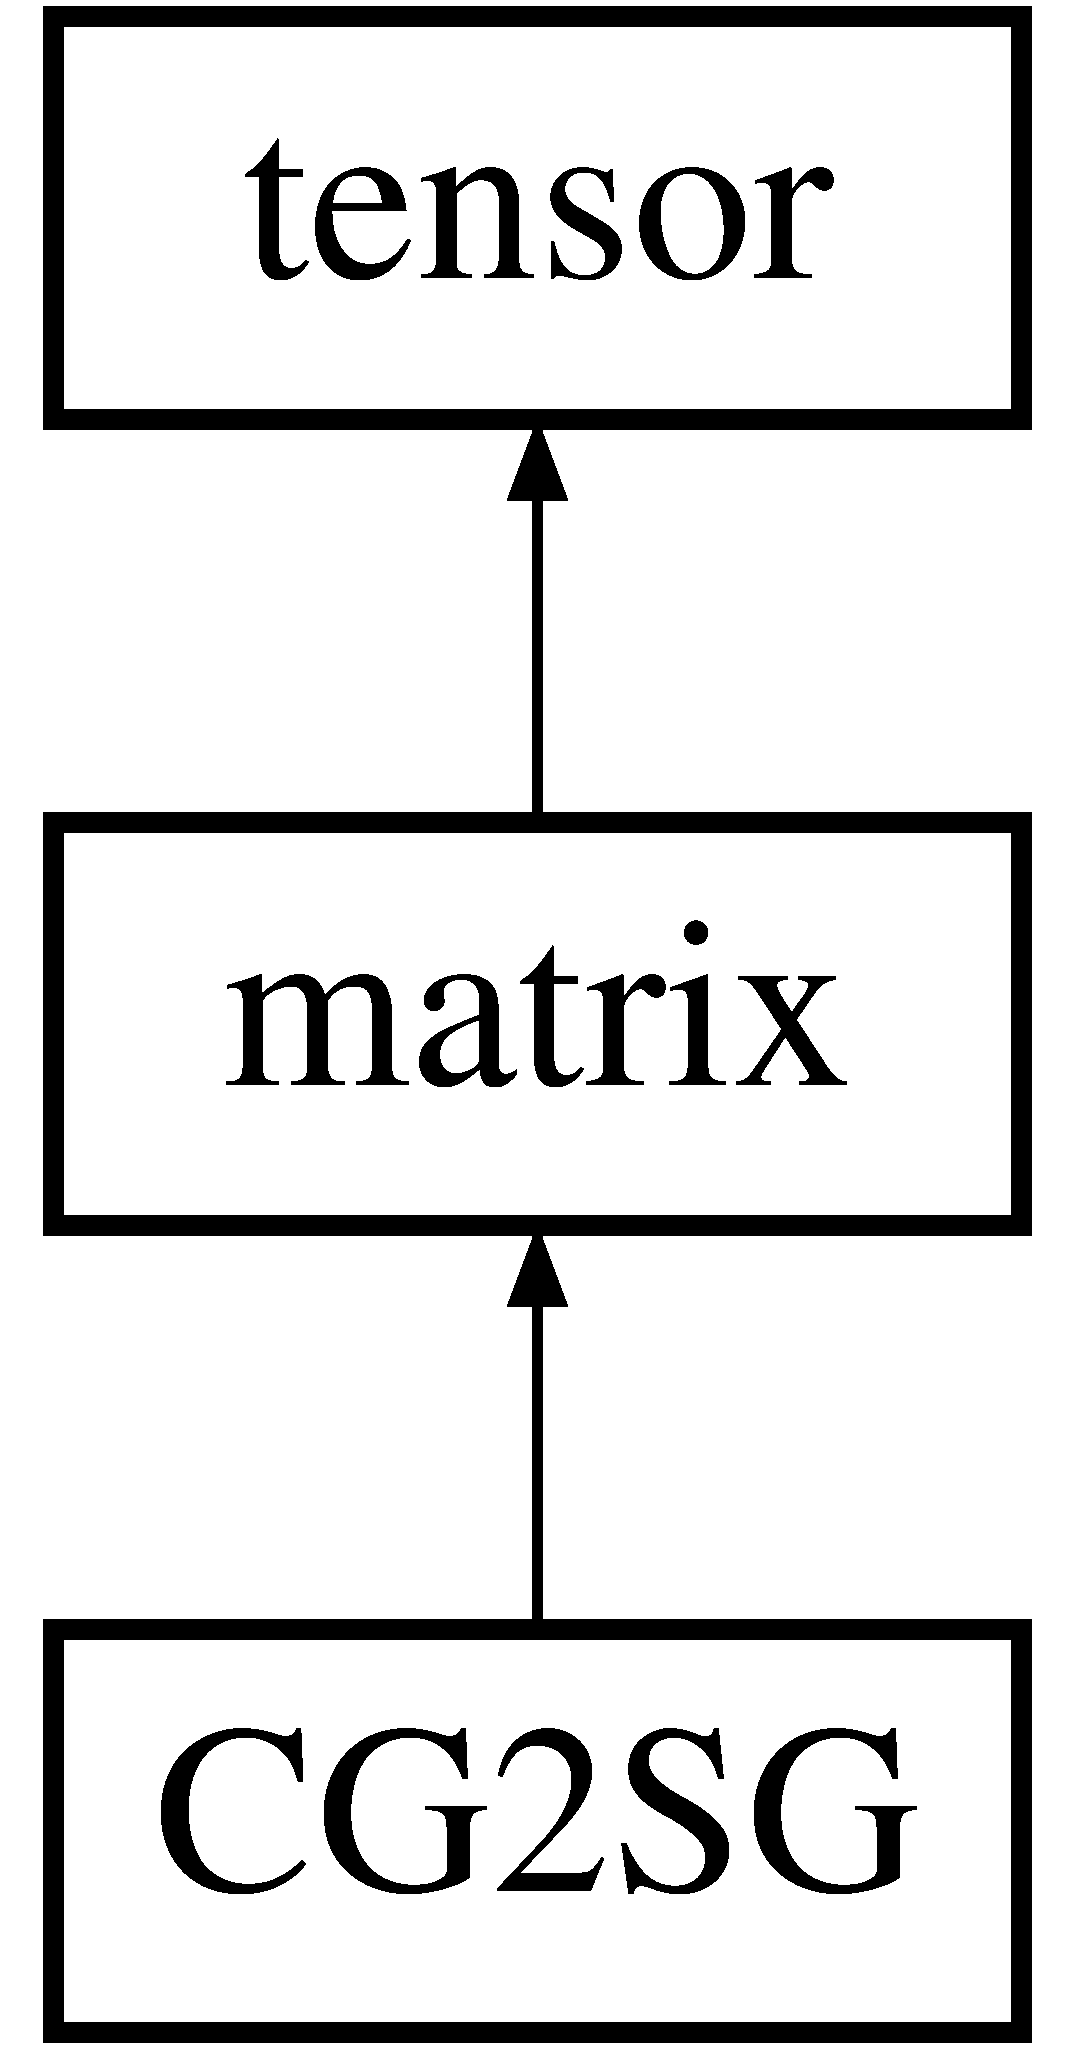
\includegraphics[height=3cm]{classJKBuilder_1_1CG2SG}
\end{center}
\end{figure}
\subsection*{Public Member Functions}
\begin{DoxyCompactItemize}
\item 
\hyperlink{classJKBuilder_1_1CG2SG_a3dd17ea7b07cd7d20b0c21010b56eb04}{CG2SG} (\hyperlink{classJKBuilder_1_1AOBasisSet}{AOBasisSet} $\ast$basis)
\begin{DoxyCompactList}\small\item\em Give an AO basis set, generates the appropriate transformation \hyperlink{classJKBuilder_1_1matrix}{matrix} to go from the CG to SG basis. \item\end{DoxyCompactList}\item 
void \hyperlink{classJKBuilder_1_1matrix_af2563817f6505e9f8a6ee5c5c209a115}{T} ()
\begin{DoxyCompactList}\small\item\em Transposes a \hyperlink{classJKBuilder_1_1matrix}{matrix} by flipping the flag (don't forget to un-\/transpose it). \item\end{DoxyCompactList}\item 
const double \& \hyperlink{classJKBuilder_1_1matrix_a9ccbac42f4eefb704f04886001f4fb3e}{operator()} (const int i, const int j) const 
\begin{DoxyCompactList}\small\item\em Returns a non-\/editable element (i,j). \item\end{DoxyCompactList}\item 
double \& \hyperlink{classJKBuilder_1_1matrix_a3d7fca183ff1c9f4c160218746f2ef31}{operator()} (const int i, const int j)
\begin{DoxyCompactList}\small\item\em Returns an editable element (i,j). \item\end{DoxyCompactList}\item 
\hyperlink{classJKBuilder_1_1matrix}{matrix} \& \hyperlink{classJKBuilder_1_1matrix_ad4799cbe4a5d07c77f41857a3ce914a2}{operator$\ast$} (const double alpha)
\begin{DoxyCompactList}\small\item\em Scales a \hyperlink{classJKBuilder_1_1matrix}{matrix} by alpha. \item\end{DoxyCompactList}\item 
void \hyperlink{classJKBuilder_1_1tensor_a0ca5cbe96d2a61f06ae4b543ef84f166}{Alloc} ()
\item 
bool \hyperlink{classJKBuilder_1_1tensor_a79c9a36acc5dbeab94033ca97971dc09}{IsSet} () const 
\begin{DoxyCompactList}\small\item\em Returns true if this \hyperlink{classJKBuilder_1_1tensor}{tensor} is allocated and DimsGood==true (roughly the equiv to asking if this is NULL). \item\end{DoxyCompactList}\item 
virtual void \hyperlink{classJKBuilder_1_1tensor_a98b1050f09da390896f964fb7a892391}{Initialize} ()
\begin{DoxyCompactList}\small\item\em Sets all elements to zero in the \hyperlink{classJKBuilder_1_1tensor}{tensor}, which obviously overwrites the contents. \item\end{DoxyCompactList}\item 
virtual void \hyperlink{classJKBuilder_1_1tensor_a10ffea2bf428adfa3e8319646c44a3c6}{Update} (const double $\ast$Tensor)
\begin{DoxyCompactList}\small\item\em Updates DaTensor so that it is the same as Tensor. \item\end{DoxyCompactList}\item 
int \hyperlink{classJKBuilder_1_1tensor_a537b2f14296e2f0e62f00e1703c5fa08}{TotalElements} ()
\item 
int \hyperlink{classJKBuilder_1_1tensor_a6bdcfca6493bc217b607317dbceb28b2}{DimI} (const int i) const 
\begin{DoxyCompactList}\small\item\em Returns dimension i (counting from 0). \item\end{DoxyCompactList}\item 
void \hyperlink{classJKBuilder_1_1tensor_ace6bcf62c74395ab9e37abc4935f66e0}{SetDimensions} (const int $\ast$DesiredDimensions)
\begin{DoxyCompactList}\small\item\em Copies the dimensions you want (DesiredDimensions), into the \hyperlink{classJKBuilder_1_1tensor_a2ce1e6e0782ddee097f2c4aa2663d3e9}{tensor::dimensions}. Overwrites the contents. \item\end{DoxyCompactList}\item 
virtual void \hyperlink{classJKBuilder_1_1tensor_a388f572c62279f839ee138a9afbdeeb5}{print} ()
\begin{DoxyCompactList}\small\item\em Debugging function that prints the \hyperlink{classJKBuilder_1_1tensor}{tensor} (current model not appropriate for a distributed \hyperlink{classJKBuilder_1_1tensor}{tensor}) to the \hyperlink{classJKBuilder_1_1printer}{printer}. \item\end{DoxyCompactList}\item 
virtual void \hyperlink{classJKBuilder_1_1tensor_a74b2fe351a5444c1325870dc6162f451}{print} (\hyperlink{classJKBuilder_1_1IOManager}{IOManager} \&output)
\begin{DoxyCompactList}\small\item\em Allows the user to select the destination of the printed \hyperlink{classJKBuilder_1_1tensor}{tensor}. \item\end{DoxyCompactList}\item 
const double \& \hyperlink{classJKBuilder_1_1tensor_a4f0dc1b84b580cec49500c70f87e084a}{operator\mbox{[}$\,$\mbox{]}} (const int i) const 
\begin{DoxyCompactList}\small\item\em Returns a non-\/modifiable element i of the \hyperlink{classJKBuilder_1_1tensor}{tensor}. \item\end{DoxyCompactList}\item 
double \& \hyperlink{classJKBuilder_1_1tensor_a38c9fed6b117f7cf8b76785648d76b62}{operator\mbox{[}$\,$\mbox{]}} (const int i)
\begin{DoxyCompactList}\small\item\em Returns a modifiable element i of the \hyperlink{classJKBuilder_1_1tensor}{tensor}. \item\end{DoxyCompactList}\item 
bool \hyperlink{classJKBuilder_1_1tensor_a10ae0b61e655854d12c6465d2b9e3506}{operator==} (const \hyperlink{classJKBuilder_1_1tensor}{tensor} \&other)
\begin{DoxyCompactList}\small\item\em Returns true iff this \hyperlink{classJKBuilder_1_1tensor}{tensor} is equal to the other one. \item\end{DoxyCompactList}\item 
bool \hyperlink{classJKBuilder_1_1tensor_a9b42dd835ddf2eb1a26b5d525b59b2b8}{operator!=} (const \hyperlink{classJKBuilder_1_1tensor}{tensor} \&other)
\begin{DoxyCompactList}\small\item\em Returns the opposite of operator==. \item\end{DoxyCompactList}\item 
const double $\ast$ \hyperlink{classJKBuilder_1_1tensor_a6a4e024f566d3bf9ba32a349afc5bbcf}{Address} () const 
\begin{DoxyCompactList}\small\item\em Returns the starting address of the actual data so that pointers can just be passed. \item\end{DoxyCompactList}\item 
double $\ast$ \hyperlink{classJKBuilder_1_1tensor_ac982d9eb84092bfc13694448dd824cbc}{Address} ()
\end{DoxyCompactItemize}
\subsection*{Protected Member Functions}
\begin{DoxyCompactItemize}
\item 
bool \hyperlink{classJKBuilder_1_1tensor_a6e72344440b411f433eb50171648c2d0}{DimsGood} () const 
\begin{DoxyCompactList}\small\item\em Returns true if the dimensions appear set (dimensions!=NULL \&\& dimensions\mbox{[}i\mbox{]}$>$0 for all i). \item\end{DoxyCompactList}\end{DoxyCompactItemize}
\subsection*{Protected Attributes}
\begin{DoxyCompactItemize}
\item 
bool \hyperlink{classJKBuilder_1_1matrix_a77fa48e57c519482de2ec7ec182b16ef}{IsTransposed}
\begin{DoxyCompactList}\small\item\em A flag that tells us if our \hyperlink{classJKBuilder_1_1matrix}{matrix} is transposed. \item\end{DoxyCompactList}\item 
int \hyperlink{classJKBuilder_1_1tensor_a6cfd95afd0afebd625b889fb6e58371c}{rank}
\begin{DoxyCompactList}\small\item\em This is the rank of the \hyperlink{classJKBuilder_1_1tensor}{tensor}. \item\end{DoxyCompactList}\item 
double $\ast$ \hyperlink{classJKBuilder_1_1tensor_a91f7b1e58c0e5d1a49ddb8b80ab7790e}{DaTensor}
\begin{DoxyCompactList}\small\item\em Realistically we are going to want to use this for doubles, so I am not declaring this a template. \item\end{DoxyCompactList}\item 
int \hyperlink{classJKBuilder_1_1tensor_a23ae6a00bed19d2ad34d439636e797da}{nelements}
\begin{DoxyCompactList}\small\item\em This is the total number of elements in the \hyperlink{classJKBuilder_1_1tensor}{tensor}. \item\end{DoxyCompactList}\item 
int $\ast$ \hyperlink{classJKBuilder_1_1tensor_a2ce1e6e0782ddee097f2c4aa2663d3e9}{dimensions}
\begin{DoxyCompactList}\small\item\em This is the array of \hyperlink{classJKBuilder_1_1tensor}{tensor} dimensions (row,column). \item\end{DoxyCompactList}\end{DoxyCompactItemize}
\subsection*{Private Member Functions}
\begin{DoxyCompactItemize}
\item 
double \hyperlink{classJKBuilder_1_1CG2SG_a755586288e38b18e91f6e2437f979789}{GetC} (int L, int M, int Lx, int Ly, int Lz)
\begin{DoxyCompactList}\small\item\em Returns the appropriate coefficient. \item\end{DoxyCompactList}\end{DoxyCompactItemize}


\subsection{Detailed Description}
This class handles the transformation from Cartesian Gaussians to Spherical Gaussians. Note: That I use the abbreviations CG=Cartesian Gaussian and SG=Spherical Gaussian regularly throughout this class. 

\subsection{Constructor \& Destructor Documentation}
\hypertarget{classJKBuilder_1_1CG2SG_a3dd17ea7b07cd7d20b0c21010b56eb04}{
\index{JKBuilder::CG2SG@{JKBuilder::CG2SG}!CG2SG@{CG2SG}}
\index{CG2SG@{CG2SG}!JKBuilder::CG2SG@{JKBuilder::CG2SG}}
\subsubsection[{CG2SG}]{\setlength{\rightskip}{0pt plus 5cm}{\bf CG2SG} ({\bf AOBasisSet} $\ast$ {\em basis})}}
\label{classJKBuilder_1_1CG2SG_a3dd17ea7b07cd7d20b0c21010b56eb04}


Give an AO basis set, generates the appropriate transformation \hyperlink{classJKBuilder_1_1matrix}{matrix} to go from the CG to SG basis. 

\subsection{Member Function Documentation}
\hypertarget{classJKBuilder_1_1CG2SG_a755586288e38b18e91f6e2437f979789}{
\index{JKBuilder::CG2SG@{JKBuilder::CG2SG}!GetC@{GetC}}
\index{GetC@{GetC}!JKBuilder::CG2SG@{JKBuilder::CG2SG}}
\subsubsection[{GetC}]{\setlength{\rightskip}{0pt plus 5cm}double GetC (int {\em L}, \/  int {\em M}, \/  int {\em Lx}, \/  int {\em Ly}, \/  int {\em Lz})\hspace{0.3cm}{\ttfamily  \mbox{[}private\mbox{]}}}}
\label{classJKBuilder_1_1CG2SG_a755586288e38b18e91f6e2437f979789}


Returns the appropriate coefficient. This returns the real component, not the complex. I use the convention that +M returns the positive linear combination and -\/M returns the negative combination


\begin{DoxyParams}{Parameters}
\item[\mbox{$\leftarrow$} {\em L}]The total Angular momentum \item[\mbox{$\leftarrow$} {\em M}]The projection of the Angular momentum \item[\mbox{$\leftarrow$} {\em Lx}]The x component of L \item[\mbox{$\leftarrow$} {\em Ly}]The y component of L \item[\mbox{$\leftarrow$} {\em Lz}]The z component of L \end{DoxyParams}
\hypertarget{classJKBuilder_1_1matrix_af2563817f6505e9f8a6ee5c5c209a115}{
\index{JKBuilder::CG2SG@{JKBuilder::CG2SG}!T@{T}}
\index{T@{T}!JKBuilder::CG2SG@{JKBuilder::CG2SG}}
\subsubsection[{T}]{\setlength{\rightskip}{0pt plus 5cm}void T ()\hspace{0.3cm}{\ttfamily  \mbox{[}inherited\mbox{]}}}}
\label{classJKBuilder_1_1matrix_af2563817f6505e9f8a6ee5c5c209a115}


Transposes a \hyperlink{classJKBuilder_1_1matrix}{matrix} by flipping the flag (don't forget to un-\/transpose it). \hypertarget{classJKBuilder_1_1matrix_a9ccbac42f4eefb704f04886001f4fb3e}{
\index{JKBuilder::CG2SG@{JKBuilder::CG2SG}!operator()@{operator()}}
\index{operator()@{operator()}!JKBuilder::CG2SG@{JKBuilder::CG2SG}}
\subsubsection[{operator()}]{\setlength{\rightskip}{0pt plus 5cm}const double \& operator() (const int {\em i}, \/  const int {\em j}) const\hspace{0.3cm}{\ttfamily  \mbox{[}inherited\mbox{]}}}}
\label{classJKBuilder_1_1matrix_a9ccbac42f4eefb704f04886001f4fb3e}


Returns a non-\/editable element (i,j). 

Reimplemented in \hyperlink{classJKBuilder_1_1SymmMatrix_a9ccbac42f4eefb704f04886001f4fb3e}{SymmMatrix}.\hypertarget{classJKBuilder_1_1matrix_a3d7fca183ff1c9f4c160218746f2ef31}{
\index{JKBuilder::CG2SG@{JKBuilder::CG2SG}!operator()@{operator()}}
\index{operator()@{operator()}!JKBuilder::CG2SG@{JKBuilder::CG2SG}}
\subsubsection[{operator()}]{\setlength{\rightskip}{0pt plus 5cm}double \& operator() (const int {\em i}, \/  const int {\em j})\hspace{0.3cm}{\ttfamily  \mbox{[}inherited\mbox{]}}}}
\label{classJKBuilder_1_1matrix_a3d7fca183ff1c9f4c160218746f2ef31}


Returns an editable element (i,j). 

Reimplemented in \hyperlink{classJKBuilder_1_1SymmMatrix_a3d7fca183ff1c9f4c160218746f2ef31}{SymmMatrix}.\hypertarget{classJKBuilder_1_1matrix_ad4799cbe4a5d07c77f41857a3ce914a2}{
\index{JKBuilder::CG2SG@{JKBuilder::CG2SG}!operator$\ast$@{operator$\ast$}}
\index{operator$\ast$@{operator$\ast$}!JKBuilder::CG2SG@{JKBuilder::CG2SG}}
\subsubsection[{operator$\ast$}]{\setlength{\rightskip}{0pt plus 5cm}{\bf matrix} \& operator$\ast$ (const double {\em alpha})\hspace{0.3cm}{\ttfamily  \mbox{[}inherited\mbox{]}}}}
\label{classJKBuilder_1_1matrix_ad4799cbe4a5d07c77f41857a3ce914a2}


Scales a \hyperlink{classJKBuilder_1_1matrix}{matrix} by alpha. \hypertarget{classJKBuilder_1_1tensor_a6e72344440b411f433eb50171648c2d0}{
\index{JKBuilder::CG2SG@{JKBuilder::CG2SG}!DimsGood@{DimsGood}}
\index{DimsGood@{DimsGood}!JKBuilder::CG2SG@{JKBuilder::CG2SG}}
\subsubsection[{DimsGood}]{\setlength{\rightskip}{0pt plus 5cm}bool DimsGood () const\hspace{0.3cm}{\ttfamily  \mbox{[}protected, inherited\mbox{]}}}}
\label{classJKBuilder_1_1tensor_a6e72344440b411f433eb50171648c2d0}


Returns true if the dimensions appear set (dimensions!=NULL \&\& dimensions\mbox{[}i\mbox{]}$>$0 for all i). \hypertarget{classJKBuilder_1_1tensor_a0ca5cbe96d2a61f06ae4b543ef84f166}{
\index{JKBuilder::CG2SG@{JKBuilder::CG2SG}!Alloc@{Alloc}}
\index{Alloc@{Alloc}!JKBuilder::CG2SG@{JKBuilder::CG2SG}}
\subsubsection[{Alloc}]{\setlength{\rightskip}{0pt plus 5cm}void Alloc ()\hspace{0.3cm}{\ttfamily  \mbox{[}inherited\mbox{]}}}}
\label{classJKBuilder_1_1tensor_a0ca5cbe96d2a61f06ae4b543ef84f166}
The following function can never be virtual because base operations of the Tensor depend on them The actual memory allocation call, if DaTensor==NULL allocates the memory \hypertarget{classJKBuilder_1_1tensor_a79c9a36acc5dbeab94033ca97971dc09}{
\index{JKBuilder::CG2SG@{JKBuilder::CG2SG}!IsSet@{IsSet}}
\index{IsSet@{IsSet}!JKBuilder::CG2SG@{JKBuilder::CG2SG}}
\subsubsection[{IsSet}]{\setlength{\rightskip}{0pt plus 5cm}bool IsSet () const\hspace{0.3cm}{\ttfamily  \mbox{[}inherited\mbox{]}}}}
\label{classJKBuilder_1_1tensor_a79c9a36acc5dbeab94033ca97971dc09}


Returns true if this \hyperlink{classJKBuilder_1_1tensor}{tensor} is allocated and DimsGood==true (roughly the equiv to asking if this is NULL). \hypertarget{classJKBuilder_1_1tensor_a98b1050f09da390896f964fb7a892391}{
\index{JKBuilder::CG2SG@{JKBuilder::CG2SG}!Initialize@{Initialize}}
\index{Initialize@{Initialize}!JKBuilder::CG2SG@{JKBuilder::CG2SG}}
\subsubsection[{Initialize}]{\setlength{\rightskip}{0pt plus 5cm}void Initialize ()\hspace{0.3cm}{\ttfamily  \mbox{[}virtual, inherited\mbox{]}}}}
\label{classJKBuilder_1_1tensor_a98b1050f09da390896f964fb7a892391}


Sets all elements to zero in the \hyperlink{classJKBuilder_1_1tensor}{tensor}, which obviously overwrites the contents. 

Reimplemented in \hyperlink{classJKBuilder_1_1DistributedMatrix_a98b1050f09da390896f964fb7a892391}{DistributedMatrix}.\hypertarget{classJKBuilder_1_1tensor_a10ffea2bf428adfa3e8319646c44a3c6}{
\index{JKBuilder::CG2SG@{JKBuilder::CG2SG}!Update@{Update}}
\index{Update@{Update}!JKBuilder::CG2SG@{JKBuilder::CG2SG}}
\subsubsection[{Update}]{\setlength{\rightskip}{0pt plus 5cm}void Update (const double $\ast$ {\em Tensor})\hspace{0.3cm}{\ttfamily  \mbox{[}virtual, inherited\mbox{]}}}}
\label{classJKBuilder_1_1tensor_a10ffea2bf428adfa3e8319646c44a3c6}


Updates DaTensor so that it is the same as Tensor. Update always takes the full Tensor, not a block of it. It is child class's jobs to scatter the data if need be. 

Reimplemented in \hyperlink{classJKBuilder_1_1DistributedMatrix_a6a378face23ba83b2431cb08e8519066}{DistributedMatrix}.\hypertarget{classJKBuilder_1_1tensor_a537b2f14296e2f0e62f00e1703c5fa08}{
\index{JKBuilder::CG2SG@{JKBuilder::CG2SG}!TotalElements@{TotalElements}}
\index{TotalElements@{TotalElements}!JKBuilder::CG2SG@{JKBuilder::CG2SG}}
\subsubsection[{TotalElements}]{\setlength{\rightskip}{0pt plus 5cm}int TotalElements ()\hspace{0.3cm}{\ttfamily  \mbox{[}inherited\mbox{]}}}}
\label{classJKBuilder_1_1tensor_a537b2f14296e2f0e62f00e1703c5fa08}
\hypertarget{classJKBuilder_1_1tensor_a6bdcfca6493bc217b607317dbceb28b2}{
\index{JKBuilder::CG2SG@{JKBuilder::CG2SG}!DimI@{DimI}}
\index{DimI@{DimI}!JKBuilder::CG2SG@{JKBuilder::CG2SG}}
\subsubsection[{DimI}]{\setlength{\rightskip}{0pt plus 5cm}int DimI (const int {\em i}) const\hspace{0.3cm}{\ttfamily  \mbox{[}inherited\mbox{]}}}}
\label{classJKBuilder_1_1tensor_a6bdcfca6493bc217b607317dbceb28b2}


Returns dimension i (counting from 0). \hypertarget{classJKBuilder_1_1tensor_ace6bcf62c74395ab9e37abc4935f66e0}{
\index{JKBuilder::CG2SG@{JKBuilder::CG2SG}!SetDimensions@{SetDimensions}}
\index{SetDimensions@{SetDimensions}!JKBuilder::CG2SG@{JKBuilder::CG2SG}}
\subsubsection[{SetDimensions}]{\setlength{\rightskip}{0pt plus 5cm}void SetDimensions (const int $\ast$ {\em DesiredDimensions})\hspace{0.3cm}{\ttfamily  \mbox{[}inherited\mbox{]}}}}
\label{classJKBuilder_1_1tensor_ace6bcf62c74395ab9e37abc4935f66e0}


Copies the dimensions you want (DesiredDimensions), into the \hyperlink{classJKBuilder_1_1tensor_a2ce1e6e0782ddee097f2c4aa2663d3e9}{tensor::dimensions}. Overwrites the contents. \hypertarget{classJKBuilder_1_1tensor_a388f572c62279f839ee138a9afbdeeb5}{
\index{JKBuilder::CG2SG@{JKBuilder::CG2SG}!print@{print}}
\index{print@{print}!JKBuilder::CG2SG@{JKBuilder::CG2SG}}
\subsubsection[{print}]{\setlength{\rightskip}{0pt plus 5cm}void print ()\hspace{0.3cm}{\ttfamily  \mbox{[}virtual, inherited\mbox{]}}}}
\label{classJKBuilder_1_1tensor_a388f572c62279f839ee138a9afbdeeb5}


Debugging function that prints the \hyperlink{classJKBuilder_1_1tensor}{tensor} (current model not appropriate for a distributed \hyperlink{classJKBuilder_1_1tensor}{tensor}) to the \hyperlink{classJKBuilder_1_1printer}{printer}. 

Reimplemented in \hyperlink{classJKBuilder_1_1DistributedMatrix_a388f572c62279f839ee138a9afbdeeb5}{DistributedMatrix}.\hypertarget{classJKBuilder_1_1tensor_a74b2fe351a5444c1325870dc6162f451}{
\index{JKBuilder::CG2SG@{JKBuilder::CG2SG}!print@{print}}
\index{print@{print}!JKBuilder::CG2SG@{JKBuilder::CG2SG}}
\subsubsection[{print}]{\setlength{\rightskip}{0pt plus 5cm}void print ({\bf IOManager} \& {\em output})\hspace{0.3cm}{\ttfamily  \mbox{[}virtual, inherited\mbox{]}}}}
\label{classJKBuilder_1_1tensor_a74b2fe351a5444c1325870dc6162f451}


Allows the user to select the destination of the printed \hyperlink{classJKBuilder_1_1tensor}{tensor}. 

Reimplemented in \hyperlink{classJKBuilder_1_1DistributedMatrix_a74b2fe351a5444c1325870dc6162f451}{DistributedMatrix}.\hypertarget{classJKBuilder_1_1tensor_a4f0dc1b84b580cec49500c70f87e084a}{
\index{JKBuilder::CG2SG@{JKBuilder::CG2SG}!operator\mbox{[}\mbox{]}@{operator[]}}
\index{operator\mbox{[}\mbox{]}@{operator[]}!JKBuilder::CG2SG@{JKBuilder::CG2SG}}
\subsubsection[{operator[]}]{\setlength{\rightskip}{0pt plus 5cm}const double \& operator\mbox{[}$\,$\mbox{]} (const int {\em i}) const\hspace{0.3cm}{\ttfamily  \mbox{[}inherited\mbox{]}}}}
\label{classJKBuilder_1_1tensor_a4f0dc1b84b580cec49500c70f87e084a}


Returns a non-\/modifiable element i of the \hyperlink{classJKBuilder_1_1tensor}{tensor}. \hypertarget{classJKBuilder_1_1tensor_a38c9fed6b117f7cf8b76785648d76b62}{
\index{JKBuilder::CG2SG@{JKBuilder::CG2SG}!operator\mbox{[}\mbox{]}@{operator[]}}
\index{operator\mbox{[}\mbox{]}@{operator[]}!JKBuilder::CG2SG@{JKBuilder::CG2SG}}
\subsubsection[{operator[]}]{\setlength{\rightskip}{0pt plus 5cm}double \& operator\mbox{[}$\,$\mbox{]} (const int {\em i})\hspace{0.3cm}{\ttfamily  \mbox{[}inherited\mbox{]}}}}
\label{classJKBuilder_1_1tensor_a38c9fed6b117f7cf8b76785648d76b62}


Returns a modifiable element i of the \hyperlink{classJKBuilder_1_1tensor}{tensor}. \hypertarget{classJKBuilder_1_1tensor_a10ae0b61e655854d12c6465d2b9e3506}{
\index{JKBuilder::CG2SG@{JKBuilder::CG2SG}!operator==@{operator==}}
\index{operator==@{operator==}!JKBuilder::CG2SG@{JKBuilder::CG2SG}}
\subsubsection[{operator==}]{\setlength{\rightskip}{0pt plus 5cm}bool operator== (const {\bf tensor} \& {\em other})\hspace{0.3cm}{\ttfamily  \mbox{[}inherited\mbox{]}}}}
\label{classJKBuilder_1_1tensor_a10ae0b61e655854d12c6465d2b9e3506}


Returns true iff this \hyperlink{classJKBuilder_1_1tensor}{tensor} is equal to the other one. \hypertarget{classJKBuilder_1_1tensor_a9b42dd835ddf2eb1a26b5d525b59b2b8}{
\index{JKBuilder::CG2SG@{JKBuilder::CG2SG}!operator!=@{operator!=}}
\index{operator!=@{operator!=}!JKBuilder::CG2SG@{JKBuilder::CG2SG}}
\subsubsection[{operator!=}]{\setlength{\rightskip}{0pt plus 5cm}bool operator!= (const {\bf tensor} \& {\em other})\hspace{0.3cm}{\ttfamily  \mbox{[}inherited\mbox{]}}}}
\label{classJKBuilder_1_1tensor_a9b42dd835ddf2eb1a26b5d525b59b2b8}


Returns the opposite of operator==. \hypertarget{classJKBuilder_1_1tensor_a6a4e024f566d3bf9ba32a349afc5bbcf}{
\index{JKBuilder::CG2SG@{JKBuilder::CG2SG}!Address@{Address}}
\index{Address@{Address}!JKBuilder::CG2SG@{JKBuilder::CG2SG}}
\subsubsection[{Address}]{\setlength{\rightskip}{0pt plus 5cm}const double $\ast$ Address () const\hspace{0.3cm}{\ttfamily  \mbox{[}inherited\mbox{]}}}}
\label{classJKBuilder_1_1tensor_a6a4e024f566d3bf9ba32a349afc5bbcf}


Returns the starting address of the actual data so that pointers can just be passed. \hypertarget{classJKBuilder_1_1tensor_ac982d9eb84092bfc13694448dd824cbc}{
\index{JKBuilder::CG2SG@{JKBuilder::CG2SG}!Address@{Address}}
\index{Address@{Address}!JKBuilder::CG2SG@{JKBuilder::CG2SG}}
\subsubsection[{Address}]{\setlength{\rightskip}{0pt plus 5cm}double $\ast$ Address ()\hspace{0.3cm}{\ttfamily  \mbox{[}inherited\mbox{]}}}}
\label{classJKBuilder_1_1tensor_ac982d9eb84092bfc13694448dd824cbc}


\subsection{Member Data Documentation}
\hypertarget{classJKBuilder_1_1matrix_a77fa48e57c519482de2ec7ec182b16ef}{
\index{JKBuilder::CG2SG@{JKBuilder::CG2SG}!IsTransposed@{IsTransposed}}
\index{IsTransposed@{IsTransposed}!JKBuilder::CG2SG@{JKBuilder::CG2SG}}
\subsubsection[{IsTransposed}]{\setlength{\rightskip}{0pt plus 5cm}bool {\bf IsTransposed}\hspace{0.3cm}{\ttfamily  \mbox{[}protected, inherited\mbox{]}}}}
\label{classJKBuilder_1_1matrix_a77fa48e57c519482de2ec7ec182b16ef}


A flag that tells us if our \hyperlink{classJKBuilder_1_1matrix}{matrix} is transposed. \hypertarget{classJKBuilder_1_1tensor_a6cfd95afd0afebd625b889fb6e58371c}{
\index{JKBuilder::CG2SG@{JKBuilder::CG2SG}!rank@{rank}}
\index{rank@{rank}!JKBuilder::CG2SG@{JKBuilder::CG2SG}}
\subsubsection[{rank}]{\setlength{\rightskip}{0pt plus 5cm}int {\bf rank}\hspace{0.3cm}{\ttfamily  \mbox{[}protected, inherited\mbox{]}}}}
\label{classJKBuilder_1_1tensor_a6cfd95afd0afebd625b889fb6e58371c}


This is the rank of the \hyperlink{classJKBuilder_1_1tensor}{tensor}. \hypertarget{classJKBuilder_1_1tensor_a91f7b1e58c0e5d1a49ddb8b80ab7790e}{
\index{JKBuilder::CG2SG@{JKBuilder::CG2SG}!DaTensor@{DaTensor}}
\index{DaTensor@{DaTensor}!JKBuilder::CG2SG@{JKBuilder::CG2SG}}
\subsubsection[{DaTensor}]{\setlength{\rightskip}{0pt plus 5cm}double$\ast$ {\bf DaTensor}\hspace{0.3cm}{\ttfamily  \mbox{[}protected, inherited\mbox{]}}}}
\label{classJKBuilder_1_1tensor_a91f7b1e58c0e5d1a49ddb8b80ab7790e}


Realistically we are going to want to use this for doubles, so I am not declaring this a template. \hypertarget{classJKBuilder_1_1tensor_a23ae6a00bed19d2ad34d439636e797da}{
\index{JKBuilder::CG2SG@{JKBuilder::CG2SG}!nelements@{nelements}}
\index{nelements@{nelements}!JKBuilder::CG2SG@{JKBuilder::CG2SG}}
\subsubsection[{nelements}]{\setlength{\rightskip}{0pt plus 5cm}int {\bf nelements}\hspace{0.3cm}{\ttfamily  \mbox{[}protected, inherited\mbox{]}}}}
\label{classJKBuilder_1_1tensor_a23ae6a00bed19d2ad34d439636e797da}


This is the total number of elements in the \hyperlink{classJKBuilder_1_1tensor}{tensor}. \hypertarget{classJKBuilder_1_1tensor_a2ce1e6e0782ddee097f2c4aa2663d3e9}{
\index{JKBuilder::CG2SG@{JKBuilder::CG2SG}!dimensions@{dimensions}}
\index{dimensions@{dimensions}!JKBuilder::CG2SG@{JKBuilder::CG2SG}}
\subsubsection[{dimensions}]{\setlength{\rightskip}{0pt plus 5cm}int$\ast$ {\bf dimensions}\hspace{0.3cm}{\ttfamily  \mbox{[}protected, inherited\mbox{]}}}}
\label{classJKBuilder_1_1tensor_a2ce1e6e0782ddee097f2c4aa2663d3e9}


This is the array of \hyperlink{classJKBuilder_1_1tensor}{tensor} dimensions (row,column). These dimensions are for the whole object, not blocks of it or anything else like that. What this means is that for say a 12 by 12 \hyperlink{classJKBuilder_1_1matrix}{matrix} distributed in 6 by 6 blocks these values are 12, not 6. 

The documentation for this class was generated from the following files:\begin{DoxyCompactItemize}
\item 
src/\hyperlink{CG2SG_8h}{CG2SG.h}\item 
src/\hyperlink{CG2SG_8cpp}{CG2SG.cpp}\end{DoxyCompactItemize}

\hypertarget{classGTFock_1_1DistGTFock}{
\section{DistGTFock Class Reference}
\label{classGTFock_1_1DistGTFock}\index{GTFock::DistGTFock@{GTFock::DistGTFock}}
}


{\ttfamily \#include $<$DistGTFock.h$>$}Inheritance diagram for DistGTFock::\begin{figure}[H]
\begin{center}
\leavevmode
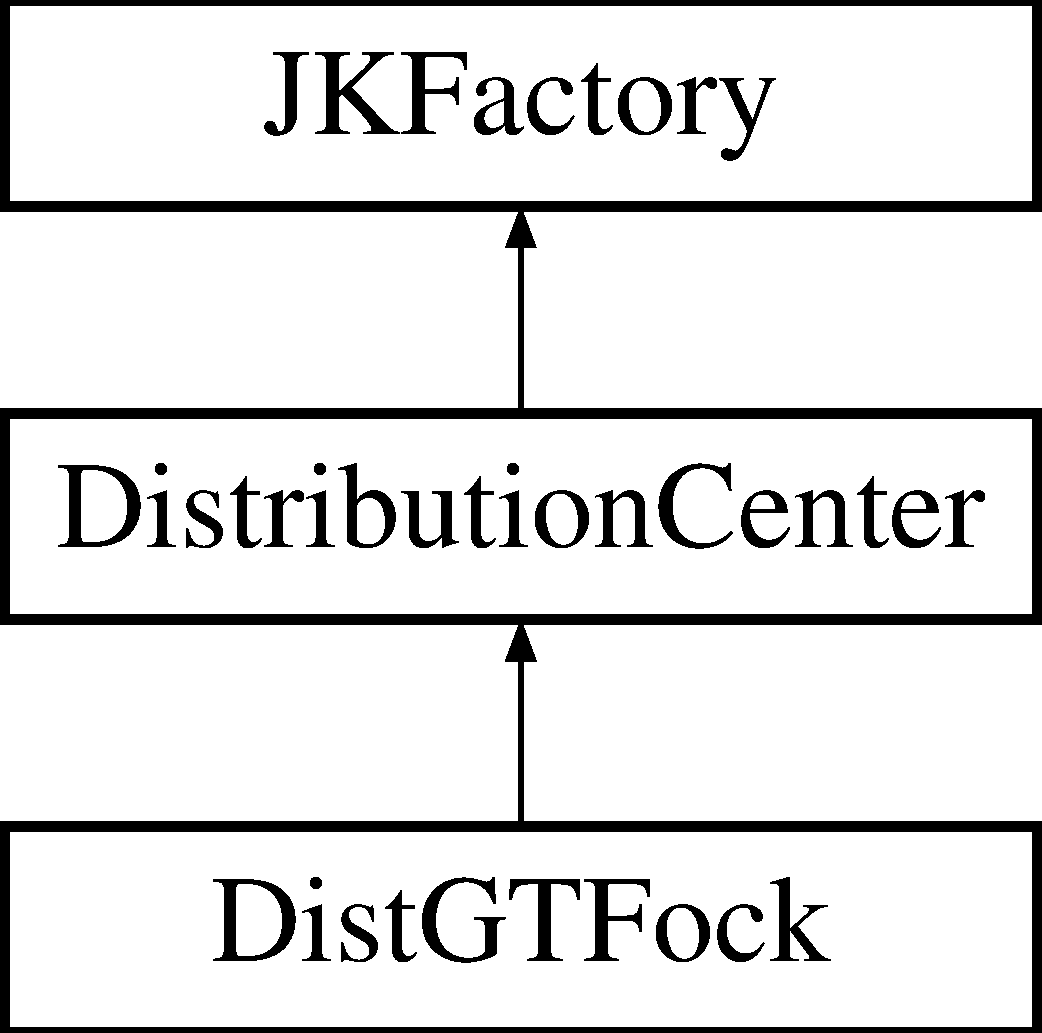
\includegraphics[height=3cm]{classGTFock_1_1DistGTFock}
\end{center}
\end{figure}
\subsection*{Public Member Functions}
\begin{DoxyCompactItemize}
\item 
void \hyperlink{classGTFock_1_1DistGTFock_aea85d0b3d84e8e52819e8a15201e078a}{BuildJK} (const double $\ast$DensityMatrix, \hyperlink{namespaceJKBuilder_aef21bc37b7cf7bc5ebb5a48628db8d0f}{JKBuilder::SharedSymJKMatrix} \&J\_\-Matrix, \hyperlink{namespaceJKBuilder_aef21bc37b7cf7bc5ebb5a48628db8d0f}{JKBuilder::SharedSymJKMatrix} \&K\_\-Matrix)
\begin{DoxyCompactList}\small\item\em The function actually in charge of building the J and K matrices. \item\end{DoxyCompactList}\item 
\hyperlink{classGTFock_1_1DistGTFock_a98b483024f3677552f2fca216363b66d}{DistGTFock} (\hyperlink{classJKBuilder_1_1AOBasisSet}{JKBuilder::AOBasisSet} $\ast$basis, \hyperlink{classJKBuilder_1_1molecule__class}{JKBuilder::molecule\_\-class} $\ast$molecule)
\begin{DoxyCompactList}\small\item\em Allocates memory for MPI. \item\end{DoxyCompactList}\item 
\hyperlink{classGTFock_1_1DistGTFock_aacafefb187ed3acf152e0b2f75cca49b}{$\sim$DistGTFock} ()
\begin{DoxyCompactList}\small\item\em Deletes the memory for MPI. \item\end{DoxyCompactList}\end{DoxyCompactItemize}
\subsection*{Protected Attributes}
\begin{DoxyCompactItemize}
\item 
MPIManager $\ast$ \hyperlink{classJKBuilder_1_1DistributionCenter_a3753afd7c89e077643a274ed7c4e9129}{MPI}
\begin{DoxyCompactList}\small\item\em This is the object in charge of managing the parallelism. \item\end{DoxyCompactList}\item 
std::vector$<$ SharedDistMatrix $>$ \hyperlink{classJKBuilder_1_1DistributionCenter_aea5bfaa6247d7c03edf480fa8ecdd929}{rho}
\begin{DoxyCompactList}\small\item\em The distributed density \hyperlink{classJKBuilder_1_1matrix}{matrix}. \item\end{DoxyCompactList}\item 
std::vector$<$ SharedDistMatrix $>$ \hyperlink{classJKBuilder_1_1DistributionCenter_a83e7fc1320b7071187dce35322e659b2}{J}
\begin{DoxyCompactList}\small\item\em The distributed Coloumb \hyperlink{classJKBuilder_1_1matrix}{matrix}. \item\end{DoxyCompactList}\item 
std::vector$<$ SharedDistMatrix $>$ \hyperlink{classJKBuilder_1_1DistributionCenter_a36d7716ac07910f43805622922c1fb93}{K}
\begin{DoxyCompactList}\small\item\em The distributed Exchange \hyperlink{classJKBuilder_1_1matrix}{matrix}. \item\end{DoxyCompactList}\end{DoxyCompactItemize}
\subsection*{Private Member Functions}
\begin{DoxyCompactItemize}
\item 
void \hyperlink{classGTFock_1_1DistGTFock_af1268d1c5fac4a061b995c267bf9f219}{CopyBasis} (\hyperlink{classJKBuilder_1_1AOBasisSet}{JKBuilder::AOBasisSet} $\ast$basis, const \hyperlink{classJKBuilder_1_1molecule__class}{JKBuilder::molecule\_\-class} $\ast$molecule)
\begin{DoxyCompactList}\small\item\em Copies it's data into a \hyperlink{namespaceGTFock}{GTFock} basis set object. \item\end{DoxyCompactList}\item 
void \hyperlink{classGTFock_1_1DistGTFock_a0da100e6aeb49168e1c88c7cfae6e976}{SetUp} (\hyperlink{classJKBuilder_1_1AOBasisSet}{JKBuilder::AOBasisSet} $\ast$basis, const \hyperlink{classJKBuilder_1_1molecule__class}{JKBuilder::molecule\_\-class} $\ast$molecule)
\begin{DoxyCompactList}\small\item\em The function in charge of establishing our link to the \hyperlink{namespaceGTFock}{GTFock} library. \item\end{DoxyCompactList}\end{DoxyCompactItemize}
\subsection*{Private Attributes}
\begin{DoxyCompactItemize}
\item 
BasisSet $\ast$ \hyperlink{classGTFock_1_1DistGTFock_acf01612812393db2711417ca40f2d629}{GTbasis}
\begin{DoxyCompactList}\small\item\em This sort of BasisSet object is here because it is used by the \hyperlink{namespaceGTFock}{GTFock} Library. \item\end{DoxyCompactList}\item 
PFock $\ast$ \hyperlink{classGTFock_1_1DistGTFock_a4d2250740bf39e3a0f585c264a79f902}{Fock}
\begin{DoxyCompactList}\small\item\em This is the \hyperlink{namespaceGTFock}{GTFock} Fock object. \item\end{DoxyCompactList}\item 
\_\-purf\_\-t $\ast$ \hyperlink{classGTFock_1_1DistGTFock_a67a350742753030caf0b3e66027d6d4b}{purf}
\begin{DoxyCompactList}\small\item\em This is the \hyperlink{namespaceGTFock}{GTFock} Density object. \item\end{DoxyCompactList}\item 
int \hyperlink{classGTFock_1_1DistGTFock_a13c5e6c87e46d3ddac36125f8c824736}{nblks\_\-fock}
\begin{DoxyCompactList}\small\item\em This is some parameter that enters into the routine. I am not sure what it does, but was told to set it to 5. \item\end{DoxyCompactList}\end{DoxyCompactItemize}


\subsection{Constructor \& Destructor Documentation}
\hypertarget{classGTFock_1_1DistGTFock_a98b483024f3677552f2fca216363b66d}{
\index{GTFock::DistGTFock@{GTFock::DistGTFock}!DistGTFock@{DistGTFock}}
\index{DistGTFock@{DistGTFock}!GTFock::DistGTFock@{GTFock::DistGTFock}}
\subsubsection[{DistGTFock}]{\setlength{\rightskip}{0pt plus 5cm}{\bf DistGTFock} ({\bf JKBuilder::AOBasisSet} $\ast$ {\em basis}, \/  {\bf JKBuilder::molecule\_\-class} $\ast$ {\em molecule})}}
\label{classGTFock_1_1DistGTFock_a98b483024f3677552f2fca216363b66d}


Allocates memory for MPI. \hypertarget{classGTFock_1_1DistGTFock_aacafefb187ed3acf152e0b2f75cca49b}{
\index{GTFock::DistGTFock@{GTFock::DistGTFock}!$\sim$DistGTFock@{$\sim$DistGTFock}}
\index{$\sim$DistGTFock@{$\sim$DistGTFock}!GTFock::DistGTFock@{GTFock::DistGTFock}}
\subsubsection[{$\sim$DistGTFock}]{\setlength{\rightskip}{0pt plus 5cm}$\sim${\bf DistGTFock} ()}}
\label{classGTFock_1_1DistGTFock_aacafefb187ed3acf152e0b2f75cca49b}


Deletes the memory for MPI. 

\subsection{Member Function Documentation}
\hypertarget{classGTFock_1_1DistGTFock_af1268d1c5fac4a061b995c267bf9f219}{
\index{GTFock::DistGTFock@{GTFock::DistGTFock}!CopyBasis@{CopyBasis}}
\index{CopyBasis@{CopyBasis}!GTFock::DistGTFock@{GTFock::DistGTFock}}
\subsubsection[{CopyBasis}]{\setlength{\rightskip}{0pt plus 5cm}void CopyBasis ({\bf JKBuilder::AOBasisSet} $\ast$ {\em basis}, \/  const {\bf JKBuilder::molecule\_\-class} $\ast$ {\em molecule})\hspace{0.3cm}{\ttfamily  \mbox{[}private\mbox{]}}}}
\label{classGTFock_1_1DistGTFock_af1268d1c5fac4a061b995c267bf9f219}


Copies it's data into a \hyperlink{namespaceGTFock}{GTFock} basis set object. \hypertarget{classGTFock_1_1DistGTFock_a0da100e6aeb49168e1c88c7cfae6e976}{
\index{GTFock::DistGTFock@{GTFock::DistGTFock}!SetUp@{SetUp}}
\index{SetUp@{SetUp}!GTFock::DistGTFock@{GTFock::DistGTFock}}
\subsubsection[{SetUp}]{\setlength{\rightskip}{0pt plus 5cm}void SetUp ({\bf JKBuilder::AOBasisSet} $\ast$ {\em basis}, \/  const {\bf JKBuilder::molecule\_\-class} $\ast$ {\em molecule})\hspace{0.3cm}{\ttfamily  \mbox{[}private\mbox{]}}}}
\label{classGTFock_1_1DistGTFock_a0da100e6aeb49168e1c88c7cfae6e976}


The function in charge of establishing our link to the \hyperlink{namespaceGTFock}{GTFock} library. The \hyperlink{namespaceGTFock}{GTFock} library needs several things from us to get started: it's basis set object, the number of processors per row and column of the Fock matrix, and some basic info about the problem. This routine takes care of that. \hypertarget{classGTFock_1_1DistGTFock_aea85d0b3d84e8e52819e8a15201e078a}{
\index{GTFock::DistGTFock@{GTFock::DistGTFock}!BuildJK@{BuildJK}}
\index{BuildJK@{BuildJK}!GTFock::DistGTFock@{GTFock::DistGTFock}}
\subsubsection[{BuildJK}]{\setlength{\rightskip}{0pt plus 5cm}void BuildJK (const double $\ast$ {\em DensityMatrix}, \/  {\bf JKBuilder::SharedSymJKMatrix} \& {\em J\_\-Matrix}, \/  {\bf JKBuilder::SharedSymJKMatrix} \& {\em K\_\-Matrix})\hspace{0.3cm}{\ttfamily  \mbox{[}virtual\mbox{]}}}}
\label{classGTFock_1_1DistGTFock_aea85d0b3d84e8e52819e8a15201e078a}


The function actually in charge of building the J and K matrices. This function first updates the density matrix to be the one given to it. Next, it computes J and K and returns them as matrix objects.


\begin{DoxyParams}{Parameters}
\item[\mbox{$\leftarrow$} {\em DensityMatrix}]The density matrix \item[\mbox{$\rightarrow$} {\em J}]The Coulomb matrix corresponding to DensityMatrix \item[\mbox{$\rightarrow$} {\em K}]The Exchange matrix corresponding to DensityMatrix \end{DoxyParams}


Implements \hyperlink{classJKBuilder_1_1JKFactory_ae253b309dafe3ce003fdabfd315318b8}{JKFactory}.

\subsection{Member Data Documentation}
\hypertarget{classGTFock_1_1DistGTFock_acf01612812393db2711417ca40f2d629}{
\index{GTFock::DistGTFock@{GTFock::DistGTFock}!GTbasis@{GTbasis}}
\index{GTbasis@{GTbasis}!GTFock::DistGTFock@{GTFock::DistGTFock}}
\subsubsection[{GTbasis}]{\setlength{\rightskip}{0pt plus 5cm}BasisSet$\ast$ {\bf GTbasis}\hspace{0.3cm}{\ttfamily  \mbox{[}private\mbox{]}}}}
\label{classGTFock_1_1DistGTFock_acf01612812393db2711417ca40f2d629}


This sort of BasisSet object is here because it is used by the \hyperlink{namespaceGTFock}{GTFock} Library. \hypertarget{classGTFock_1_1DistGTFock_a4d2250740bf39e3a0f585c264a79f902}{
\index{GTFock::DistGTFock@{GTFock::DistGTFock}!Fock@{Fock}}
\index{Fock@{Fock}!GTFock::DistGTFock@{GTFock::DistGTFock}}
\subsubsection[{Fock}]{\setlength{\rightskip}{0pt plus 5cm}PFock$\ast$ {\bf Fock}\hspace{0.3cm}{\ttfamily  \mbox{[}private\mbox{]}}}}
\label{classGTFock_1_1DistGTFock_a4d2250740bf39e3a0f585c264a79f902}


This is the \hyperlink{namespaceGTFock}{GTFock} Fock object. \hypertarget{classGTFock_1_1DistGTFock_a67a350742753030caf0b3e66027d6d4b}{
\index{GTFock::DistGTFock@{GTFock::DistGTFock}!purf@{purf}}
\index{purf@{purf}!GTFock::DistGTFock@{GTFock::DistGTFock}}
\subsubsection[{purf}]{\setlength{\rightskip}{0pt plus 5cm}\_\-purf\_\-t$\ast$ {\bf purf}\hspace{0.3cm}{\ttfamily  \mbox{[}private\mbox{]}}}}
\label{classGTFock_1_1DistGTFock_a67a350742753030caf0b3e66027d6d4b}


This is the \hyperlink{namespaceGTFock}{GTFock} Density object. \hypertarget{classGTFock_1_1DistGTFock_a13c5e6c87e46d3ddac36125f8c824736}{
\index{GTFock::DistGTFock@{GTFock::DistGTFock}!nblks\_\-fock@{nblks\_\-fock}}
\index{nblks\_\-fock@{nblks\_\-fock}!GTFock::DistGTFock@{GTFock::DistGTFock}}
\subsubsection[{nblks\_\-fock}]{\setlength{\rightskip}{0pt plus 5cm}int {\bf nblks\_\-fock}\hspace{0.3cm}{\ttfamily  \mbox{[}private\mbox{]}}}}
\label{classGTFock_1_1DistGTFock_a13c5e6c87e46d3ddac36125f8c824736}


This is some parameter that enters into the routine. I am not sure what it does, but was told to set it to 5. \hypertarget{classJKBuilder_1_1DistributionCenter_a3753afd7c89e077643a274ed7c4e9129}{
\index{GTFock::DistGTFock@{GTFock::DistGTFock}!MPI@{MPI}}
\index{MPI@{MPI}!GTFock::DistGTFock@{GTFock::DistGTFock}}
\subsubsection[{MPI}]{\setlength{\rightskip}{0pt plus 5cm}MPIManager$\ast$ {\bf MPI}\hspace{0.3cm}{\ttfamily  \mbox{[}protected, inherited\mbox{]}}}}
\label{classJKBuilder_1_1DistributionCenter_a3753afd7c89e077643a274ed7c4e9129}


This is the object in charge of managing the parallelism. \hypertarget{classJKBuilder_1_1DistributionCenter_aea5bfaa6247d7c03edf480fa8ecdd929}{
\index{GTFock::DistGTFock@{GTFock::DistGTFock}!rho@{rho}}
\index{rho@{rho}!GTFock::DistGTFock@{GTFock::DistGTFock}}
\subsubsection[{rho}]{\setlength{\rightskip}{0pt plus 5cm}std::vector$<$SharedDistMatrix$>$ {\bf rho}\hspace{0.3cm}{\ttfamily  \mbox{[}protected, inherited\mbox{]}}}}
\label{classJKBuilder_1_1DistributionCenter_aea5bfaa6247d7c03edf480fa8ecdd929}


The distributed density \hyperlink{classJKBuilder_1_1matrix}{matrix}. \hypertarget{classJKBuilder_1_1DistributionCenter_a83e7fc1320b7071187dce35322e659b2}{
\index{GTFock::DistGTFock@{GTFock::DistGTFock}!J@{J}}
\index{J@{J}!GTFock::DistGTFock@{GTFock::DistGTFock}}
\subsubsection[{J}]{\setlength{\rightskip}{0pt plus 5cm}std::vector$<$SharedDistMatrix$>$ {\bf J}\hspace{0.3cm}{\ttfamily  \mbox{[}protected, inherited\mbox{]}}}}
\label{classJKBuilder_1_1DistributionCenter_a83e7fc1320b7071187dce35322e659b2}


The distributed Coloumb \hyperlink{classJKBuilder_1_1matrix}{matrix}. \hypertarget{classJKBuilder_1_1DistributionCenter_a36d7716ac07910f43805622922c1fb93}{
\index{GTFock::DistGTFock@{GTFock::DistGTFock}!K@{K}}
\index{K@{K}!GTFock::DistGTFock@{GTFock::DistGTFock}}
\subsubsection[{K}]{\setlength{\rightskip}{0pt plus 5cm}std::vector$<$SharedDistMatrix$>$ {\bf K}\hspace{0.3cm}{\ttfamily  \mbox{[}protected, inherited\mbox{]}}}}
\label{classJKBuilder_1_1DistributionCenter_a36d7716ac07910f43805622922c1fb93}


The distributed Exchange \hyperlink{classJKBuilder_1_1matrix}{matrix}. 

The documentation for this class was generated from the following files:\begin{DoxyCompactItemize}
\item 
src/\hyperlink{DistGTFock_8h}{DistGTFock.h}\item 
src/\hyperlink{DistGTFock_8cpp}{DistGTFock.cpp}\end{DoxyCompactItemize}

\hypertarget{classJKBuilder_1_1DistributedMatrix}{
\section{DistributedMatrix Class Reference}
\label{classJKBuilder_1_1DistributedMatrix}\index{JKBuilder::DistributedMatrix@{JKBuilder::DistributedMatrix}}
}


{\ttfamily \#include $<$DistributedMatrix.h$>$}Inheritance diagram for DistributedMatrix::\begin{figure}[H]
\begin{center}
\leavevmode
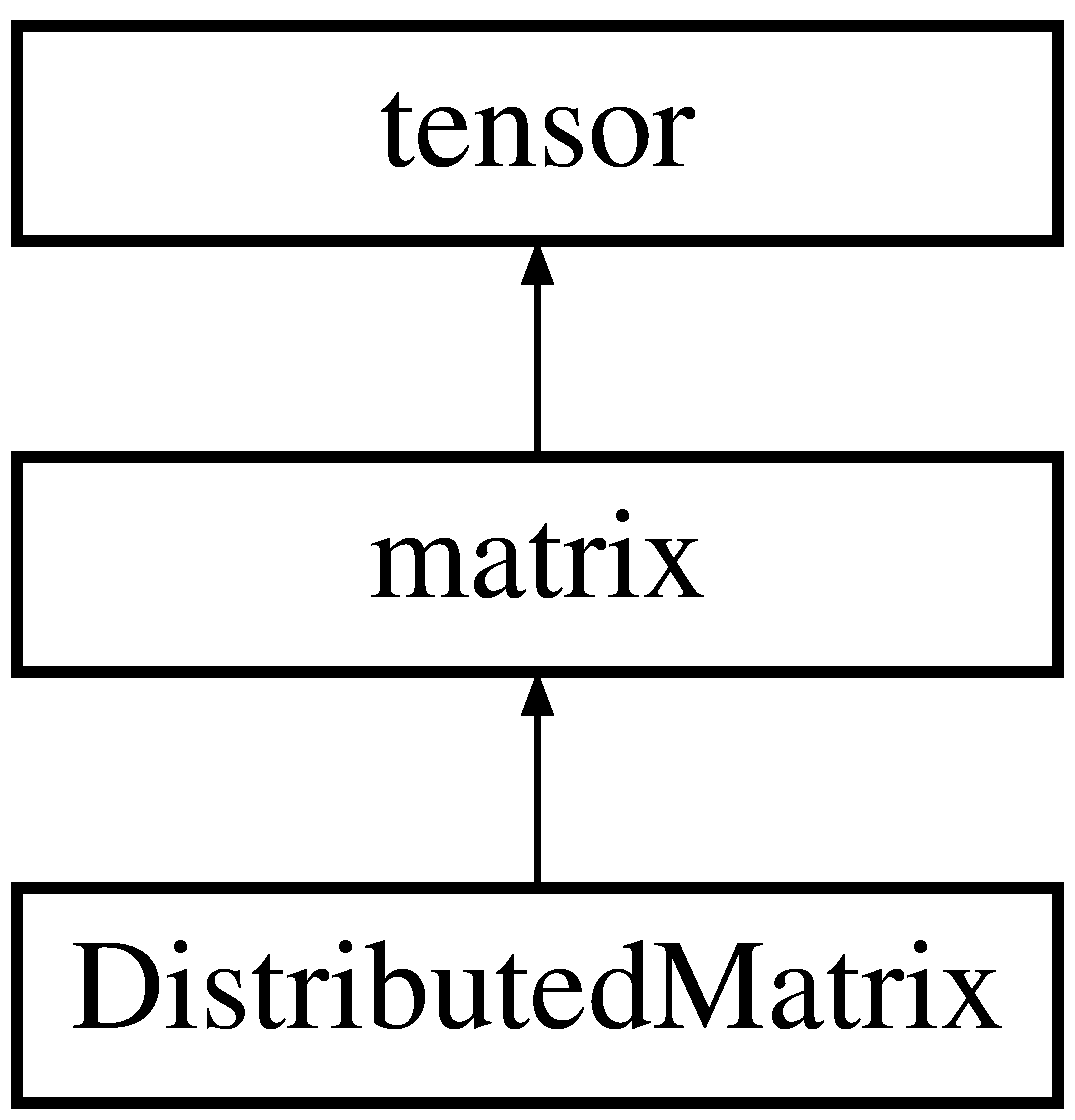
\includegraphics[height=3cm]{classJKBuilder_1_1DistributedMatrix}
\end{center}
\end{figure}
\subsection*{Public Member Functions}
\begin{DoxyCompactItemize}
\item 
void \hyperlink{classJKBuilder_1_1DistributedMatrix_a6a378face23ba83b2431cb08e8519066}{Update} (const double $\ast$DaMatrix)
\begin{DoxyCompactList}\small\item\em Sets the \hyperlink{classJKBuilder_1_1matrix}{matrix} equal to DaMatrix. \item\end{DoxyCompactList}\item 
void \hyperlink{classJKBuilder_1_1DistributedMatrix_a825e549c725b991ad81d4ea25f630d9e}{Gather} (\hyperlink{namespaceJKBuilder_ad6c4232cd3938548f4ad3a91fbc5a2e8}{SharedJKMatrix} DaMatrix)
\begin{DoxyCompactList}\small\item\em Gathers the blocks and returns the entire \hyperlink{classJKBuilder_1_1matrix}{matrix} as DaMatrix. \item\end{DoxyCompactList}\item 
void \hyperlink{classJKBuilder_1_1DistributedMatrix_a388f572c62279f839ee138a9afbdeeb5}{print} ()
\begin{DoxyCompactList}\small\item\em Debugging function that prints the \hyperlink{classJKBuilder_1_1tensor}{tensor} (current model not appropriate for a distributed \hyperlink{classJKBuilder_1_1tensor}{tensor}) to the \hyperlink{classJKBuilder_1_1printer}{printer}. \item\end{DoxyCompactList}\item 
void \hyperlink{classJKBuilder_1_1DistributedMatrix_a74b2fe351a5444c1325870dc6162f451}{print} (\hyperlink{classJKBuilder_1_1IOManager}{IOManager} \&output)
\begin{DoxyCompactList}\small\item\em Right now still calls \hyperlink{classJKBuilder_1_1DistributedMatrix_a388f572c62279f839ee138a9afbdeeb5}{print()};. \item\end{DoxyCompactList}\item 
\hyperlink{classJKBuilder_1_1DistributedMatrix_a8de5bd3fc1dd1dc2869ef78a5e3709ab}{DistributedMatrix} (const double $\ast$DaMatrix, const int n, const int m)
\item 
\hyperlink{classJKBuilder_1_1DistributedMatrix_a2573810932403629148ce0cdbb05003c}{DistributedMatrix} (const int n, const int m)
\item 
\hyperlink{classJKBuilder_1_1DistributedMatrix_a0cfeada932c8873aaea3f86b0528c62a}{$\sim$DistributedMatrix} ()
\item 
void \hyperlink{classJKBuilder_1_1matrix_af2563817f6505e9f8a6ee5c5c209a115}{T} ()
\begin{DoxyCompactList}\small\item\em Transposes a \hyperlink{classJKBuilder_1_1matrix}{matrix} by flipping the flag (don't forget to un-\/transpose it). \item\end{DoxyCompactList}\item 
const double \& \hyperlink{classJKBuilder_1_1matrix_a9ccbac42f4eefb704f04886001f4fb3e}{operator()} (const int i, const int j) const 
\begin{DoxyCompactList}\small\item\em Returns a non-\/editable element (i,j). \item\end{DoxyCompactList}\item 
double \& \hyperlink{classJKBuilder_1_1matrix_a3d7fca183ff1c9f4c160218746f2ef31}{operator()} (const int i, const int j)
\begin{DoxyCompactList}\small\item\em Returns an editable element (i,j). \item\end{DoxyCompactList}\item 
\hyperlink{classJKBuilder_1_1matrix}{matrix} \& \hyperlink{classJKBuilder_1_1matrix_ad4799cbe4a5d07c77f41857a3ce914a2}{operator$\ast$} (const double alpha)
\begin{DoxyCompactList}\small\item\em Scales a \hyperlink{classJKBuilder_1_1matrix}{matrix} by alpha. \item\end{DoxyCompactList}\item 
void \hyperlink{classJKBuilder_1_1tensor_a0ca5cbe96d2a61f06ae4b543ef84f166}{Alloc} ()
\item 
bool \hyperlink{classJKBuilder_1_1tensor_a79c9a36acc5dbeab94033ca97971dc09}{IsSet} () const 
\begin{DoxyCompactList}\small\item\em Returns true if this \hyperlink{classJKBuilder_1_1tensor}{tensor} is allocated and DimsGood==true (roughly the equiv to asking if this is NULL). \item\end{DoxyCompactList}\item 
int \hyperlink{classJKBuilder_1_1tensor_a537b2f14296e2f0e62f00e1703c5fa08}{TotalElements} ()
\item 
int \hyperlink{classJKBuilder_1_1tensor_a6bdcfca6493bc217b607317dbceb28b2}{DimI} (const int i) const 
\begin{DoxyCompactList}\small\item\em Returns dimension i (counting from 0). \item\end{DoxyCompactList}\item 
void \hyperlink{classJKBuilder_1_1tensor_ace6bcf62c74395ab9e37abc4935f66e0}{SetDimensions} (const int $\ast$DesiredDimensions)
\begin{DoxyCompactList}\small\item\em Copies the dimensions you want (DesiredDimensions), into the \hyperlink{classJKBuilder_1_1tensor_a2ce1e6e0782ddee097f2c4aa2663d3e9}{tensor::dimensions}. Overwrites the contents. \item\end{DoxyCompactList}\item 
const double \& \hyperlink{classJKBuilder_1_1tensor_a4f0dc1b84b580cec49500c70f87e084a}{operator\mbox{[}$\,$\mbox{]}} (const int i) const 
\begin{DoxyCompactList}\small\item\em Returns a non-\/modifiable element i of the \hyperlink{classJKBuilder_1_1tensor}{tensor}. \item\end{DoxyCompactList}\item 
double \& \hyperlink{classJKBuilder_1_1tensor_a38c9fed6b117f7cf8b76785648d76b62}{operator\mbox{[}$\,$\mbox{]}} (const int i)
\begin{DoxyCompactList}\small\item\em Returns a modifiable element i of the \hyperlink{classJKBuilder_1_1tensor}{tensor}. \item\end{DoxyCompactList}\item 
bool \hyperlink{classJKBuilder_1_1tensor_a10ae0b61e655854d12c6465d2b9e3506}{operator==} (const \hyperlink{classJKBuilder_1_1tensor}{tensor} \&other)
\begin{DoxyCompactList}\small\item\em Returns true iff this \hyperlink{classJKBuilder_1_1tensor}{tensor} is equal to the other one. \item\end{DoxyCompactList}\item 
bool \hyperlink{classJKBuilder_1_1tensor_a9b42dd835ddf2eb1a26b5d525b59b2b8}{operator!=} (const \hyperlink{classJKBuilder_1_1tensor}{tensor} \&other)
\begin{DoxyCompactList}\small\item\em Returns the opposite of operator==. \item\end{DoxyCompactList}\item 
const double $\ast$ \hyperlink{classJKBuilder_1_1tensor_a6a4e024f566d3bf9ba32a349afc5bbcf}{Address} () const 
\begin{DoxyCompactList}\small\item\em Returns the starting address of the actual data so that pointers can just be passed. \item\end{DoxyCompactList}\item 
double $\ast$ \hyperlink{classJKBuilder_1_1tensor_ac982d9eb84092bfc13694448dd824cbc}{Address} ()
\end{DoxyCompactItemize}
\begin{Indent}{\bf }\par
{\em \label{_amgrpd41d8cd98f00b204e9800998ecf8427e}
 }\begin{DoxyCompactItemize}
\item 
int \hyperlink{classJKBuilder_1_1DistributedMatrix_adb8ed2a17bb3d2cd8a1bb7b0d2c55b3d}{Getnprow} ()
\item 
int \hyperlink{classJKBuilder_1_1DistributedMatrix_a47943671cf60e2d66e45dbb8e83b3f73}{Getnpcol} ()
\item 
int \hyperlink{classJKBuilder_1_1DistributedMatrix_a17ad25aa4ef86883bc294bd1bd9beab2}{Getstartrow} ()
\item 
int \hyperlink{classJKBuilder_1_1DistributedMatrix_a9fe5bf62e51849a77d75cdf03144aa3a}{Getendrow} ()
\item 
int \hyperlink{classJKBuilder_1_1DistributedMatrix_a9b957ebb8465bd874870a302cb9fc1a2}{Getstartcol} ()
\item 
int \hyperlink{classJKBuilder_1_1DistributedMatrix_a800352b707ea98657805568e3c0ed8a7}{Getendcol} ()
\end{DoxyCompactItemize}
\end{Indent}
\subsection*{Protected Member Functions}
\begin{DoxyCompactItemize}
\item 
void \hyperlink{classJKBuilder_1_1DistributedMatrix_a98b1050f09da390896f964fb7a892391}{Initialize} ()
\begin{DoxyCompactList}\small\item\em Sets all elements to zero in the \hyperlink{classJKBuilder_1_1tensor}{tensor}, which obviously overwrites the contents. \item\end{DoxyCompactList}\item 
bool \hyperlink{classJKBuilder_1_1tensor_a6e72344440b411f433eb50171648c2d0}{DimsGood} () const 
\begin{DoxyCompactList}\small\item\em Returns true if the dimensions appear set (dimensions!=NULL \&\& dimensions\mbox{[}i\mbox{]}$>$0 for all i). \item\end{DoxyCompactList}\end{DoxyCompactItemize}
\subsection*{Protected Attributes}
\begin{DoxyCompactItemize}
\item 
bool \hyperlink{classJKBuilder_1_1matrix_a77fa48e57c519482de2ec7ec182b16ef}{IsTransposed}
\begin{DoxyCompactList}\small\item\em A flag that tells us if our \hyperlink{classJKBuilder_1_1matrix}{matrix} is transposed. \item\end{DoxyCompactList}\item 
int \hyperlink{classJKBuilder_1_1tensor_a6cfd95afd0afebd625b889fb6e58371c}{rank}
\begin{DoxyCompactList}\small\item\em This is the rank of the \hyperlink{classJKBuilder_1_1tensor}{tensor}. \item\end{DoxyCompactList}\item 
double $\ast$ \hyperlink{classJKBuilder_1_1tensor_a91f7b1e58c0e5d1a49ddb8b80ab7790e}{DaTensor}
\begin{DoxyCompactList}\small\item\em Realistically we are going to want to use this for doubles, so I am not declaring this a template. \item\end{DoxyCompactList}\item 
int \hyperlink{classJKBuilder_1_1tensor_a23ae6a00bed19d2ad34d439636e797da}{nelements}
\begin{DoxyCompactList}\small\item\em This is the total number of elements in the \hyperlink{classJKBuilder_1_1tensor}{tensor}. \item\end{DoxyCompactList}\item 
int $\ast$ \hyperlink{classJKBuilder_1_1tensor_a2ce1e6e0782ddee097f2c4aa2663d3e9}{dimensions}
\begin{DoxyCompactList}\small\item\em This is the array of \hyperlink{classJKBuilder_1_1tensor}{tensor} dimensions (row,column). \item\end{DoxyCompactList}\end{DoxyCompactItemize}
\subsection*{Private Member Functions}
\begin{DoxyCompactItemize}
\item 
void \hyperlink{classJKBuilder_1_1DistributedMatrix_a83da6054896e4107ab7e0c71fe0067ff}{PrintMyBlock} ()
\item 
void \hyperlink{classJKBuilder_1_1DistributedMatrix_a97f9cb6c12da83dc8006d442247a769a}{SplitProc} (int \&nrows, int \&ncols)
\begin{DoxyCompactList}\small\item\em This function splits the processors between rows and columns. \item\end{DoxyCompactList}\item 
void \hyperlink{classJKBuilder_1_1DistributedMatrix_a425fa9d0b5ab98afbe7233895795060f}{DivvyMatrix} ()
\end{DoxyCompactItemize}
\subsection*{Private Attributes}
\begin{DoxyCompactItemize}
\item 
\hyperlink{classJKBuilder_1_1MPIManager}{MPIManager} $\ast$ \hyperlink{classJKBuilder_1_1DistributedMatrix_a3753afd7c89e077643a274ed7c4e9129}{MPI}
\begin{DoxyCompactList}\small\item\em This is the MPI object managing the distributed nature of this class. \item\end{DoxyCompactList}\item 
int \hyperlink{classJKBuilder_1_1DistributedMatrix_a3580dd419b5547085d094696e5dcc7b7}{nprow}
\begin{DoxyCompactList}\small\item\em This is the number of processors per row. \item\end{DoxyCompactList}\item 
int \hyperlink{classJKBuilder_1_1DistributedMatrix_a9d55bf8e4bef97aaacf79db88a9863cc}{npcol}
\begin{DoxyCompactList}\small\item\em This is the number of processors per column. \item\end{DoxyCompactList}\item 
int $\ast$ \hyperlink{classJKBuilder_1_1DistributedMatrix_a417b5c8d480cf1688e6c403fd29fac12}{RowPerBlock}
\begin{DoxyCompactList}\small\item\em This is an array of the number of rows per row processor. \item\end{DoxyCompactList}\item 
int $\ast$ \hyperlink{classJKBuilder_1_1DistributedMatrix_a19f481b08a628ad2707b1e82bbb88e1d}{ColPerBlock}
\begin{DoxyCompactList}\small\item\em This is an array of the number of columns per column processor. \item\end{DoxyCompactList}\item 
int \hyperlink{classJKBuilder_1_1DistributedMatrix_a0870e21b7fb2685df81b50e80b22ed7b}{startrow}
\begin{DoxyCompactList}\small\item\em This is the starting row of this block. \item\end{DoxyCompactList}\item 
int \hyperlink{classJKBuilder_1_1DistributedMatrix_ac7e765f729497d4e56e0d42c5ed012a5}{endrow}
\begin{DoxyCompactList}\small\item\em This is the ending row of this block. \item\end{DoxyCompactList}\item 
int \hyperlink{classJKBuilder_1_1DistributedMatrix_a5eb542e8d134d383869bad22b844803c}{startcol}
\begin{DoxyCompactList}\small\item\em This is the starting column of this block. \item\end{DoxyCompactList}\item 
int \hyperlink{classJKBuilder_1_1DistributedMatrix_a7e502d765772134f83b51fe10b920003}{endcol}
\begin{DoxyCompactList}\small\item\em This is the ending column of this block. \item\end{DoxyCompactList}\item 
int \hyperlink{classJKBuilder_1_1DistributedMatrix_ab2111652d429fab8c160bfbec8c6b5fb}{nBlkRow}
\begin{DoxyCompactList}\small\item\em The number of rows in the block. \item\end{DoxyCompactList}\item 
int \hyperlink{classJKBuilder_1_1DistributedMatrix_aa66940e3557e3b5bb5f1b3b4b2dbc013}{nBlkCol}
\begin{DoxyCompactList}\small\item\em The number of columns in the block. \item\end{DoxyCompactList}\end{DoxyCompactItemize}


\subsection{Constructor \& Destructor Documentation}
\hypertarget{classJKBuilder_1_1DistributedMatrix_a8de5bd3fc1dd1dc2869ef78a5e3709ab}{
\index{JKBuilder::DistributedMatrix@{JKBuilder::DistributedMatrix}!DistributedMatrix@{DistributedMatrix}}
\index{DistributedMatrix@{DistributedMatrix}!JKBuilder::DistributedMatrix@{JKBuilder::DistributedMatrix}}
\subsubsection[{DistributedMatrix}]{\setlength{\rightskip}{0pt plus 5cm}{\bf DistributedMatrix} (const double $\ast$ {\em DaMatrix}, \/  const int {\em n}, \/  const int {\em m})}}
\label{classJKBuilder_1_1DistributedMatrix_a8de5bd3fc1dd1dc2869ef78a5e3709ab}
\hypertarget{classJKBuilder_1_1DistributedMatrix_a2573810932403629148ce0cdbb05003c}{
\index{JKBuilder::DistributedMatrix@{JKBuilder::DistributedMatrix}!DistributedMatrix@{DistributedMatrix}}
\index{DistributedMatrix@{DistributedMatrix}!JKBuilder::DistributedMatrix@{JKBuilder::DistributedMatrix}}
\subsubsection[{DistributedMatrix}]{\setlength{\rightskip}{0pt plus 5cm}{\bf DistributedMatrix} (const int {\em n}, \/  const int {\em m})}}
\label{classJKBuilder_1_1DistributedMatrix_a2573810932403629148ce0cdbb05003c}
\hypertarget{classJKBuilder_1_1DistributedMatrix_a0cfeada932c8873aaea3f86b0528c62a}{
\index{JKBuilder::DistributedMatrix@{JKBuilder::DistributedMatrix}!$\sim$DistributedMatrix@{$\sim$DistributedMatrix}}
\index{$\sim$DistributedMatrix@{$\sim$DistributedMatrix}!JKBuilder::DistributedMatrix@{JKBuilder::DistributedMatrix}}
\subsubsection[{$\sim$DistributedMatrix}]{\setlength{\rightskip}{0pt plus 5cm}$\sim${\bf DistributedMatrix} ()}}
\label{classJKBuilder_1_1DistributedMatrix_a0cfeada932c8873aaea3f86b0528c62a}


\subsection{Member Function Documentation}
\hypertarget{classJKBuilder_1_1DistributedMatrix_a83da6054896e4107ab7e0c71fe0067ff}{
\index{JKBuilder::DistributedMatrix@{JKBuilder::DistributedMatrix}!PrintMyBlock@{PrintMyBlock}}
\index{PrintMyBlock@{PrintMyBlock}!JKBuilder::DistributedMatrix@{JKBuilder::DistributedMatrix}}
\subsubsection[{PrintMyBlock}]{\setlength{\rightskip}{0pt plus 5cm}void PrintMyBlock ()\hspace{0.3cm}{\ttfamily  \mbox{[}private\mbox{]}}}}
\label{classJKBuilder_1_1DistributedMatrix_a83da6054896e4107ab7e0c71fe0067ff}
\hypertarget{classJKBuilder_1_1DistributedMatrix_a97f9cb6c12da83dc8006d442247a769a}{
\index{JKBuilder::DistributedMatrix@{JKBuilder::DistributedMatrix}!SplitProc@{SplitProc}}
\index{SplitProc@{SplitProc}!JKBuilder::DistributedMatrix@{JKBuilder::DistributedMatrix}}
\subsubsection[{SplitProc}]{\setlength{\rightskip}{0pt plus 5cm}void SplitProc (int \& {\em nrows}, \/  int \& {\em ncols})\hspace{0.3cm}{\ttfamily  \mbox{[}private\mbox{]}}}}
\label{classJKBuilder_1_1DistributedMatrix_a97f9cb6c12da83dc8006d442247a769a}


This function splits the processors between rows and columns. For the \hyperlink{namespaceGTFock}{GTFock} algorithm we must satisfy:

\[ N_{Total}=N_{col}N_{row},\]

where $N_{Total}$ is the number of processors totally available to us, $N_{col}$, $N_{row}$ are the number of processors being used for the columns and the rows of the J and K matrices, respectively. For maximum efficiency we want:

\[N_{col}\approx N_{row}.\]

This is trivially satisfied if $N_{Total}$ is a perfect square. Otherwise, the floor of the square root of $N_{Total}$, $N_{approx}$, is the closest (without going over) integer, approximately satisfying this condition as long as $N_{approx}$ is a factor of $N_{Total}$. If it is not, we subtract one from $N_{approx}$ and see if the result is a factor of $N_{approx}$. This is repeated until a factor is found, which in the worst case will happen by $N_{approx}=1$ if $N_{Total}$ is prime. Even for about a million processors (keyword about, I know: $\sqrt{1,000,000}=1,000$) this amounts to at worst about 1,000 subtraction and integer comparison operations, which should represent minimal computational overhead.

Because I see no reason why $N_{col}$ or $N_{row}$ should be privileged, I have set $N_{row}=N_{approx}$. This in turn means that $N_{col}\ge N_{row}\qquad\forall\ N_{approx},N_{Total}$, a point used in several places.


\begin{DoxyParams}{Parameters}
\item[\mbox{$\leftrightarrow$} {\em nrows}]The value coming in is ignored, going out the value is the number of processors that should be used per row \item[\mbox{$\leftrightarrow$} {\em ncols}]The value coming in is ignored, going out the value is the number of processors that should be used per column \end{DoxyParams}
\hypertarget{classJKBuilder_1_1DistributedMatrix_a425fa9d0b5ab98afbe7233895795060f}{
\index{JKBuilder::DistributedMatrix@{JKBuilder::DistributedMatrix}!DivvyMatrix@{DivvyMatrix}}
\index{DivvyMatrix@{DivvyMatrix}!JKBuilder::DistributedMatrix@{JKBuilder::DistributedMatrix}}
\subsubsection[{DivvyMatrix}]{\setlength{\rightskip}{0pt plus 5cm}void DivvyMatrix ()\hspace{0.3cm}{\ttfamily  \mbox{[}private\mbox{]}}}}
\label{classJKBuilder_1_1DistributedMatrix_a425fa9d0b5ab98afbe7233895795060f}
up the \hyperlink{classJKBuilder_1_1matrix}{matrix}

Given some n by m \hyperlink{classJKBuilder_1_1matrix}{matrix}, N row processors, M column processors this routine: 1. Breaks the n by m \hyperlink{classJKBuilder_1_1matrix}{matrix} into N$\ast$M blocks. -\/Blocks are assigned by process ID: $row=processID/M$ and $col=processIK\% M$ 2. Each row block will contain at most: $\left\lfloor n/N\right\rfloor$ rows and at most: $\left\lfloor m/M\right\rfloor$ columns \hypertarget{classJKBuilder_1_1DistributedMatrix_a98b1050f09da390896f964fb7a892391}{
\index{JKBuilder::DistributedMatrix@{JKBuilder::DistributedMatrix}!Initialize@{Initialize}}
\index{Initialize@{Initialize}!JKBuilder::DistributedMatrix@{JKBuilder::DistributedMatrix}}
\subsubsection[{Initialize}]{\setlength{\rightskip}{0pt plus 5cm}void Initialize ()\hspace{0.3cm}{\ttfamily  \mbox{[}protected, virtual\mbox{]}}}}
\label{classJKBuilder_1_1DistributedMatrix_a98b1050f09da390896f964fb7a892391}


Sets all elements to zero in the \hyperlink{classJKBuilder_1_1tensor}{tensor}, which obviously overwrites the contents. 

Reimplemented from \hyperlink{classJKBuilder_1_1tensor_a98b1050f09da390896f964fb7a892391}{tensor}.\hypertarget{classJKBuilder_1_1DistributedMatrix_a6a378face23ba83b2431cb08e8519066}{
\index{JKBuilder::DistributedMatrix@{JKBuilder::DistributedMatrix}!Update@{Update}}
\index{Update@{Update}!JKBuilder::DistributedMatrix@{JKBuilder::DistributedMatrix}}
\subsubsection[{Update}]{\setlength{\rightskip}{0pt plus 5cm}void Update (const double $\ast$ {\em DaMatrix})\hspace{0.3cm}{\ttfamily  \mbox{[}virtual\mbox{]}}}}
\label{classJKBuilder_1_1DistributedMatrix_a6a378face23ba83b2431cb08e8519066}


Sets the \hyperlink{classJKBuilder_1_1matrix}{matrix} equal to DaMatrix. 

Reimplemented from \hyperlink{classJKBuilder_1_1tensor_a10ffea2bf428adfa3e8319646c44a3c6}{tensor}.\hypertarget{classJKBuilder_1_1DistributedMatrix_a825e549c725b991ad81d4ea25f630d9e}{
\index{JKBuilder::DistributedMatrix@{JKBuilder::DistributedMatrix}!Gather@{Gather}}
\index{Gather@{Gather}!JKBuilder::DistributedMatrix@{JKBuilder::DistributedMatrix}}
\subsubsection[{Gather}]{\setlength{\rightskip}{0pt plus 5cm}void Gather ({\bf SharedJKMatrix} {\em DaMatrix})}}
\label{classJKBuilder_1_1DistributedMatrix_a825e549c725b991ad81d4ea25f630d9e}


Gathers the blocks and returns the entire \hyperlink{classJKBuilder_1_1matrix}{matrix} as DaMatrix. \hypertarget{classJKBuilder_1_1DistributedMatrix_a388f572c62279f839ee138a9afbdeeb5}{
\index{JKBuilder::DistributedMatrix@{JKBuilder::DistributedMatrix}!print@{print}}
\index{print@{print}!JKBuilder::DistributedMatrix@{JKBuilder::DistributedMatrix}}
\subsubsection[{print}]{\setlength{\rightskip}{0pt plus 5cm}void print ()\hspace{0.3cm}{\ttfamily  \mbox{[}virtual\mbox{]}}}}
\label{classJKBuilder_1_1DistributedMatrix_a388f572c62279f839ee138a9afbdeeb5}


Debugging function that prints the \hyperlink{classJKBuilder_1_1tensor}{tensor} (current model not appropriate for a distributed \hyperlink{classJKBuilder_1_1tensor}{tensor}) to the \hyperlink{classJKBuilder_1_1printer}{printer}. 

Reimplemented from \hyperlink{classJKBuilder_1_1tensor_a388f572c62279f839ee138a9afbdeeb5}{tensor}.\hypertarget{classJKBuilder_1_1DistributedMatrix_a74b2fe351a5444c1325870dc6162f451}{
\index{JKBuilder::DistributedMatrix@{JKBuilder::DistributedMatrix}!print@{print}}
\index{print@{print}!JKBuilder::DistributedMatrix@{JKBuilder::DistributedMatrix}}
\subsubsection[{print}]{\setlength{\rightskip}{0pt plus 5cm}void print ({\bf IOManager} \& {\em output})\hspace{0.3cm}{\ttfamily  \mbox{[}virtual\mbox{]}}}}
\label{classJKBuilder_1_1DistributedMatrix_a74b2fe351a5444c1325870dc6162f451}


Right now still calls \hyperlink{classJKBuilder_1_1DistributedMatrix_a388f572c62279f839ee138a9afbdeeb5}{print()};. 

Reimplemented from \hyperlink{classJKBuilder_1_1tensor_a74b2fe351a5444c1325870dc6162f451}{tensor}.\hypertarget{classJKBuilder_1_1DistributedMatrix_adb8ed2a17bb3d2cd8a1bb7b0d2c55b3d}{
\index{JKBuilder::DistributedMatrix@{JKBuilder::DistributedMatrix}!Getnprow@{Getnprow}}
\index{Getnprow@{Getnprow}!JKBuilder::DistributedMatrix@{JKBuilder::DistributedMatrix}}
\subsubsection[{Getnprow}]{\setlength{\rightskip}{0pt plus 5cm}int Getnprow ()}}
\label{classJKBuilder_1_1DistributedMatrix_adb8ed2a17bb3d2cd8a1bb7b0d2c55b3d}
\hypertarget{classJKBuilder_1_1DistributedMatrix_a47943671cf60e2d66e45dbb8e83b3f73}{
\index{JKBuilder::DistributedMatrix@{JKBuilder::DistributedMatrix}!Getnpcol@{Getnpcol}}
\index{Getnpcol@{Getnpcol}!JKBuilder::DistributedMatrix@{JKBuilder::DistributedMatrix}}
\subsubsection[{Getnpcol}]{\setlength{\rightskip}{0pt plus 5cm}int Getnpcol ()}}
\label{classJKBuilder_1_1DistributedMatrix_a47943671cf60e2d66e45dbb8e83b3f73}
\hypertarget{classJKBuilder_1_1DistributedMatrix_a17ad25aa4ef86883bc294bd1bd9beab2}{
\index{JKBuilder::DistributedMatrix@{JKBuilder::DistributedMatrix}!Getstartrow@{Getstartrow}}
\index{Getstartrow@{Getstartrow}!JKBuilder::DistributedMatrix@{JKBuilder::DistributedMatrix}}
\subsubsection[{Getstartrow}]{\setlength{\rightskip}{0pt plus 5cm}int Getstartrow ()}}
\label{classJKBuilder_1_1DistributedMatrix_a17ad25aa4ef86883bc294bd1bd9beab2}
\hypertarget{classJKBuilder_1_1DistributedMatrix_a9fe5bf62e51849a77d75cdf03144aa3a}{
\index{JKBuilder::DistributedMatrix@{JKBuilder::DistributedMatrix}!Getendrow@{Getendrow}}
\index{Getendrow@{Getendrow}!JKBuilder::DistributedMatrix@{JKBuilder::DistributedMatrix}}
\subsubsection[{Getendrow}]{\setlength{\rightskip}{0pt plus 5cm}int Getendrow ()}}
\label{classJKBuilder_1_1DistributedMatrix_a9fe5bf62e51849a77d75cdf03144aa3a}
\hypertarget{classJKBuilder_1_1DistributedMatrix_a9b957ebb8465bd874870a302cb9fc1a2}{
\index{JKBuilder::DistributedMatrix@{JKBuilder::DistributedMatrix}!Getstartcol@{Getstartcol}}
\index{Getstartcol@{Getstartcol}!JKBuilder::DistributedMatrix@{JKBuilder::DistributedMatrix}}
\subsubsection[{Getstartcol}]{\setlength{\rightskip}{0pt plus 5cm}int Getstartcol ()}}
\label{classJKBuilder_1_1DistributedMatrix_a9b957ebb8465bd874870a302cb9fc1a2}
\hypertarget{classJKBuilder_1_1DistributedMatrix_a800352b707ea98657805568e3c0ed8a7}{
\index{JKBuilder::DistributedMatrix@{JKBuilder::DistributedMatrix}!Getendcol@{Getendcol}}
\index{Getendcol@{Getendcol}!JKBuilder::DistributedMatrix@{JKBuilder::DistributedMatrix}}
\subsubsection[{Getendcol}]{\setlength{\rightskip}{0pt plus 5cm}int Getendcol ()}}
\label{classJKBuilder_1_1DistributedMatrix_a800352b707ea98657805568e3c0ed8a7}
\hypertarget{classJKBuilder_1_1matrix_af2563817f6505e9f8a6ee5c5c209a115}{
\index{JKBuilder::DistributedMatrix@{JKBuilder::DistributedMatrix}!T@{T}}
\index{T@{T}!JKBuilder::DistributedMatrix@{JKBuilder::DistributedMatrix}}
\subsubsection[{T}]{\setlength{\rightskip}{0pt plus 5cm}void T ()\hspace{0.3cm}{\ttfamily  \mbox{[}inherited\mbox{]}}}}
\label{classJKBuilder_1_1matrix_af2563817f6505e9f8a6ee5c5c209a115}


Transposes a \hyperlink{classJKBuilder_1_1matrix}{matrix} by flipping the flag (don't forget to un-\/transpose it). \hypertarget{classJKBuilder_1_1matrix_a9ccbac42f4eefb704f04886001f4fb3e}{
\index{JKBuilder::DistributedMatrix@{JKBuilder::DistributedMatrix}!operator()@{operator()}}
\index{operator()@{operator()}!JKBuilder::DistributedMatrix@{JKBuilder::DistributedMatrix}}
\subsubsection[{operator()}]{\setlength{\rightskip}{0pt plus 5cm}const double \& operator() (const int {\em i}, \/  const int {\em j}) const\hspace{0.3cm}{\ttfamily  \mbox{[}inherited\mbox{]}}}}
\label{classJKBuilder_1_1matrix_a9ccbac42f4eefb704f04886001f4fb3e}


Returns a non-\/editable element (i,j). 

Reimplemented in \hyperlink{classJKBuilder_1_1SymmMatrix_a9ccbac42f4eefb704f04886001f4fb3e}{SymmMatrix}.\hypertarget{classJKBuilder_1_1matrix_a3d7fca183ff1c9f4c160218746f2ef31}{
\index{JKBuilder::DistributedMatrix@{JKBuilder::DistributedMatrix}!operator()@{operator()}}
\index{operator()@{operator()}!JKBuilder::DistributedMatrix@{JKBuilder::DistributedMatrix}}
\subsubsection[{operator()}]{\setlength{\rightskip}{0pt plus 5cm}double \& operator() (const int {\em i}, \/  const int {\em j})\hspace{0.3cm}{\ttfamily  \mbox{[}inherited\mbox{]}}}}
\label{classJKBuilder_1_1matrix_a3d7fca183ff1c9f4c160218746f2ef31}


Returns an editable element (i,j). 

Reimplemented in \hyperlink{classJKBuilder_1_1SymmMatrix_a3d7fca183ff1c9f4c160218746f2ef31}{SymmMatrix}.\hypertarget{classJKBuilder_1_1matrix_ad4799cbe4a5d07c77f41857a3ce914a2}{
\index{JKBuilder::DistributedMatrix@{JKBuilder::DistributedMatrix}!operator$\ast$@{operator$\ast$}}
\index{operator$\ast$@{operator$\ast$}!JKBuilder::DistributedMatrix@{JKBuilder::DistributedMatrix}}
\subsubsection[{operator$\ast$}]{\setlength{\rightskip}{0pt plus 5cm}{\bf matrix} \& operator$\ast$ (const double {\em alpha})\hspace{0.3cm}{\ttfamily  \mbox{[}inherited\mbox{]}}}}
\label{classJKBuilder_1_1matrix_ad4799cbe4a5d07c77f41857a3ce914a2}


Scales a \hyperlink{classJKBuilder_1_1matrix}{matrix} by alpha. \hypertarget{classJKBuilder_1_1tensor_a6e72344440b411f433eb50171648c2d0}{
\index{JKBuilder::DistributedMatrix@{JKBuilder::DistributedMatrix}!DimsGood@{DimsGood}}
\index{DimsGood@{DimsGood}!JKBuilder::DistributedMatrix@{JKBuilder::DistributedMatrix}}
\subsubsection[{DimsGood}]{\setlength{\rightskip}{0pt plus 5cm}bool DimsGood () const\hspace{0.3cm}{\ttfamily  \mbox{[}protected, inherited\mbox{]}}}}
\label{classJKBuilder_1_1tensor_a6e72344440b411f433eb50171648c2d0}


Returns true if the dimensions appear set (dimensions!=NULL \&\& dimensions\mbox{[}i\mbox{]}$>$0 for all i). \hypertarget{classJKBuilder_1_1tensor_a0ca5cbe96d2a61f06ae4b543ef84f166}{
\index{JKBuilder::DistributedMatrix@{JKBuilder::DistributedMatrix}!Alloc@{Alloc}}
\index{Alloc@{Alloc}!JKBuilder::DistributedMatrix@{JKBuilder::DistributedMatrix}}
\subsubsection[{Alloc}]{\setlength{\rightskip}{0pt plus 5cm}void Alloc ()\hspace{0.3cm}{\ttfamily  \mbox{[}inherited\mbox{]}}}}
\label{classJKBuilder_1_1tensor_a0ca5cbe96d2a61f06ae4b543ef84f166}
The following function can never be virtual because base operations of the Tensor depend on them The actual memory allocation call, if DaTensor==NULL allocates the memory \hypertarget{classJKBuilder_1_1tensor_a79c9a36acc5dbeab94033ca97971dc09}{
\index{JKBuilder::DistributedMatrix@{JKBuilder::DistributedMatrix}!IsSet@{IsSet}}
\index{IsSet@{IsSet}!JKBuilder::DistributedMatrix@{JKBuilder::DistributedMatrix}}
\subsubsection[{IsSet}]{\setlength{\rightskip}{0pt plus 5cm}bool IsSet () const\hspace{0.3cm}{\ttfamily  \mbox{[}inherited\mbox{]}}}}
\label{classJKBuilder_1_1tensor_a79c9a36acc5dbeab94033ca97971dc09}


Returns true if this \hyperlink{classJKBuilder_1_1tensor}{tensor} is allocated and DimsGood==true (roughly the equiv to asking if this is NULL). \hypertarget{classJKBuilder_1_1tensor_a537b2f14296e2f0e62f00e1703c5fa08}{
\index{JKBuilder::DistributedMatrix@{JKBuilder::DistributedMatrix}!TotalElements@{TotalElements}}
\index{TotalElements@{TotalElements}!JKBuilder::DistributedMatrix@{JKBuilder::DistributedMatrix}}
\subsubsection[{TotalElements}]{\setlength{\rightskip}{0pt plus 5cm}int TotalElements ()\hspace{0.3cm}{\ttfamily  \mbox{[}inherited\mbox{]}}}}
\label{classJKBuilder_1_1tensor_a537b2f14296e2f0e62f00e1703c5fa08}
\hypertarget{classJKBuilder_1_1tensor_a6bdcfca6493bc217b607317dbceb28b2}{
\index{JKBuilder::DistributedMatrix@{JKBuilder::DistributedMatrix}!DimI@{DimI}}
\index{DimI@{DimI}!JKBuilder::DistributedMatrix@{JKBuilder::DistributedMatrix}}
\subsubsection[{DimI}]{\setlength{\rightskip}{0pt plus 5cm}int DimI (const int {\em i}) const\hspace{0.3cm}{\ttfamily  \mbox{[}inherited\mbox{]}}}}
\label{classJKBuilder_1_1tensor_a6bdcfca6493bc217b607317dbceb28b2}


Returns dimension i (counting from 0). \hypertarget{classJKBuilder_1_1tensor_ace6bcf62c74395ab9e37abc4935f66e0}{
\index{JKBuilder::DistributedMatrix@{JKBuilder::DistributedMatrix}!SetDimensions@{SetDimensions}}
\index{SetDimensions@{SetDimensions}!JKBuilder::DistributedMatrix@{JKBuilder::DistributedMatrix}}
\subsubsection[{SetDimensions}]{\setlength{\rightskip}{0pt plus 5cm}void SetDimensions (const int $\ast$ {\em DesiredDimensions})\hspace{0.3cm}{\ttfamily  \mbox{[}inherited\mbox{]}}}}
\label{classJKBuilder_1_1tensor_ace6bcf62c74395ab9e37abc4935f66e0}


Copies the dimensions you want (DesiredDimensions), into the \hyperlink{classJKBuilder_1_1tensor_a2ce1e6e0782ddee097f2c4aa2663d3e9}{tensor::dimensions}. Overwrites the contents. \hypertarget{classJKBuilder_1_1tensor_a4f0dc1b84b580cec49500c70f87e084a}{
\index{JKBuilder::DistributedMatrix@{JKBuilder::DistributedMatrix}!operator\mbox{[}\mbox{]}@{operator[]}}
\index{operator\mbox{[}\mbox{]}@{operator[]}!JKBuilder::DistributedMatrix@{JKBuilder::DistributedMatrix}}
\subsubsection[{operator[]}]{\setlength{\rightskip}{0pt plus 5cm}const double \& operator\mbox{[}$\,$\mbox{]} (const int {\em i}) const\hspace{0.3cm}{\ttfamily  \mbox{[}inherited\mbox{]}}}}
\label{classJKBuilder_1_1tensor_a4f0dc1b84b580cec49500c70f87e084a}


Returns a non-\/modifiable element i of the \hyperlink{classJKBuilder_1_1tensor}{tensor}. \hypertarget{classJKBuilder_1_1tensor_a38c9fed6b117f7cf8b76785648d76b62}{
\index{JKBuilder::DistributedMatrix@{JKBuilder::DistributedMatrix}!operator\mbox{[}\mbox{]}@{operator[]}}
\index{operator\mbox{[}\mbox{]}@{operator[]}!JKBuilder::DistributedMatrix@{JKBuilder::DistributedMatrix}}
\subsubsection[{operator[]}]{\setlength{\rightskip}{0pt plus 5cm}double \& operator\mbox{[}$\,$\mbox{]} (const int {\em i})\hspace{0.3cm}{\ttfamily  \mbox{[}inherited\mbox{]}}}}
\label{classJKBuilder_1_1tensor_a38c9fed6b117f7cf8b76785648d76b62}


Returns a modifiable element i of the \hyperlink{classJKBuilder_1_1tensor}{tensor}. \hypertarget{classJKBuilder_1_1tensor_a10ae0b61e655854d12c6465d2b9e3506}{
\index{JKBuilder::DistributedMatrix@{JKBuilder::DistributedMatrix}!operator==@{operator==}}
\index{operator==@{operator==}!JKBuilder::DistributedMatrix@{JKBuilder::DistributedMatrix}}
\subsubsection[{operator==}]{\setlength{\rightskip}{0pt plus 5cm}bool operator== (const {\bf tensor} \& {\em other})\hspace{0.3cm}{\ttfamily  \mbox{[}inherited\mbox{]}}}}
\label{classJKBuilder_1_1tensor_a10ae0b61e655854d12c6465d2b9e3506}


Returns true iff this \hyperlink{classJKBuilder_1_1tensor}{tensor} is equal to the other one. \hypertarget{classJKBuilder_1_1tensor_a9b42dd835ddf2eb1a26b5d525b59b2b8}{
\index{JKBuilder::DistributedMatrix@{JKBuilder::DistributedMatrix}!operator!=@{operator!=}}
\index{operator!=@{operator!=}!JKBuilder::DistributedMatrix@{JKBuilder::DistributedMatrix}}
\subsubsection[{operator!=}]{\setlength{\rightskip}{0pt plus 5cm}bool operator!= (const {\bf tensor} \& {\em other})\hspace{0.3cm}{\ttfamily  \mbox{[}inherited\mbox{]}}}}
\label{classJKBuilder_1_1tensor_a9b42dd835ddf2eb1a26b5d525b59b2b8}


Returns the opposite of operator==. \hypertarget{classJKBuilder_1_1tensor_a6a4e024f566d3bf9ba32a349afc5bbcf}{
\index{JKBuilder::DistributedMatrix@{JKBuilder::DistributedMatrix}!Address@{Address}}
\index{Address@{Address}!JKBuilder::DistributedMatrix@{JKBuilder::DistributedMatrix}}
\subsubsection[{Address}]{\setlength{\rightskip}{0pt plus 5cm}const double $\ast$ Address () const\hspace{0.3cm}{\ttfamily  \mbox{[}inherited\mbox{]}}}}
\label{classJKBuilder_1_1tensor_a6a4e024f566d3bf9ba32a349afc5bbcf}


Returns the starting address of the actual data so that pointers can just be passed. \hypertarget{classJKBuilder_1_1tensor_ac982d9eb84092bfc13694448dd824cbc}{
\index{JKBuilder::DistributedMatrix@{JKBuilder::DistributedMatrix}!Address@{Address}}
\index{Address@{Address}!JKBuilder::DistributedMatrix@{JKBuilder::DistributedMatrix}}
\subsubsection[{Address}]{\setlength{\rightskip}{0pt plus 5cm}double $\ast$ Address ()\hspace{0.3cm}{\ttfamily  \mbox{[}inherited\mbox{]}}}}
\label{classJKBuilder_1_1tensor_ac982d9eb84092bfc13694448dd824cbc}


\subsection{Member Data Documentation}
\hypertarget{classJKBuilder_1_1DistributedMatrix_a3753afd7c89e077643a274ed7c4e9129}{
\index{JKBuilder::DistributedMatrix@{JKBuilder::DistributedMatrix}!MPI@{MPI}}
\index{MPI@{MPI}!JKBuilder::DistributedMatrix@{JKBuilder::DistributedMatrix}}
\subsubsection[{MPI}]{\setlength{\rightskip}{0pt plus 5cm}{\bf MPIManager}$\ast$ {\bf MPI}\hspace{0.3cm}{\ttfamily  \mbox{[}private\mbox{]}}}}
\label{classJKBuilder_1_1DistributedMatrix_a3753afd7c89e077643a274ed7c4e9129}


This is the MPI object managing the distributed nature of this class. \hypertarget{classJKBuilder_1_1DistributedMatrix_a3580dd419b5547085d094696e5dcc7b7}{
\index{JKBuilder::DistributedMatrix@{JKBuilder::DistributedMatrix}!nprow@{nprow}}
\index{nprow@{nprow}!JKBuilder::DistributedMatrix@{JKBuilder::DistributedMatrix}}
\subsubsection[{nprow}]{\setlength{\rightskip}{0pt plus 5cm}int {\bf nprow}\hspace{0.3cm}{\ttfamily  \mbox{[}private\mbox{]}}}}
\label{classJKBuilder_1_1DistributedMatrix_a3580dd419b5547085d094696e5dcc7b7}


This is the number of processors per row. \hypertarget{classJKBuilder_1_1DistributedMatrix_a9d55bf8e4bef97aaacf79db88a9863cc}{
\index{JKBuilder::DistributedMatrix@{JKBuilder::DistributedMatrix}!npcol@{npcol}}
\index{npcol@{npcol}!JKBuilder::DistributedMatrix@{JKBuilder::DistributedMatrix}}
\subsubsection[{npcol}]{\setlength{\rightskip}{0pt plus 5cm}int {\bf npcol}\hspace{0.3cm}{\ttfamily  \mbox{[}private\mbox{]}}}}
\label{classJKBuilder_1_1DistributedMatrix_a9d55bf8e4bef97aaacf79db88a9863cc}


This is the number of processors per column. \hypertarget{classJKBuilder_1_1DistributedMatrix_a417b5c8d480cf1688e6c403fd29fac12}{
\index{JKBuilder::DistributedMatrix@{JKBuilder::DistributedMatrix}!RowPerBlock@{RowPerBlock}}
\index{RowPerBlock@{RowPerBlock}!JKBuilder::DistributedMatrix@{JKBuilder::DistributedMatrix}}
\subsubsection[{RowPerBlock}]{\setlength{\rightskip}{0pt plus 5cm}int$\ast$ {\bf RowPerBlock}\hspace{0.3cm}{\ttfamily  \mbox{[}private\mbox{]}}}}
\label{classJKBuilder_1_1DistributedMatrix_a417b5c8d480cf1688e6c403fd29fac12}


This is an array of the number of rows per row processor. \hypertarget{classJKBuilder_1_1DistributedMatrix_a19f481b08a628ad2707b1e82bbb88e1d}{
\index{JKBuilder::DistributedMatrix@{JKBuilder::DistributedMatrix}!ColPerBlock@{ColPerBlock}}
\index{ColPerBlock@{ColPerBlock}!JKBuilder::DistributedMatrix@{JKBuilder::DistributedMatrix}}
\subsubsection[{ColPerBlock}]{\setlength{\rightskip}{0pt plus 5cm}int$\ast$ {\bf ColPerBlock}\hspace{0.3cm}{\ttfamily  \mbox{[}private\mbox{]}}}}
\label{classJKBuilder_1_1DistributedMatrix_a19f481b08a628ad2707b1e82bbb88e1d}


This is an array of the number of columns per column processor. \hypertarget{classJKBuilder_1_1DistributedMatrix_a0870e21b7fb2685df81b50e80b22ed7b}{
\index{JKBuilder::DistributedMatrix@{JKBuilder::DistributedMatrix}!startrow@{startrow}}
\index{startrow@{startrow}!JKBuilder::DistributedMatrix@{JKBuilder::DistributedMatrix}}
\subsubsection[{startrow}]{\setlength{\rightskip}{0pt plus 5cm}int {\bf startrow}\hspace{0.3cm}{\ttfamily  \mbox{[}private\mbox{]}}}}
\label{classJKBuilder_1_1DistributedMatrix_a0870e21b7fb2685df81b50e80b22ed7b}


This is the starting row of this block. \hypertarget{classJKBuilder_1_1DistributedMatrix_ac7e765f729497d4e56e0d42c5ed012a5}{
\index{JKBuilder::DistributedMatrix@{JKBuilder::DistributedMatrix}!endrow@{endrow}}
\index{endrow@{endrow}!JKBuilder::DistributedMatrix@{JKBuilder::DistributedMatrix}}
\subsubsection[{endrow}]{\setlength{\rightskip}{0pt plus 5cm}int {\bf endrow}\hspace{0.3cm}{\ttfamily  \mbox{[}private\mbox{]}}}}
\label{classJKBuilder_1_1DistributedMatrix_ac7e765f729497d4e56e0d42c5ed012a5}


This is the ending row of this block. \hypertarget{classJKBuilder_1_1DistributedMatrix_a5eb542e8d134d383869bad22b844803c}{
\index{JKBuilder::DistributedMatrix@{JKBuilder::DistributedMatrix}!startcol@{startcol}}
\index{startcol@{startcol}!JKBuilder::DistributedMatrix@{JKBuilder::DistributedMatrix}}
\subsubsection[{startcol}]{\setlength{\rightskip}{0pt plus 5cm}int {\bf startcol}\hspace{0.3cm}{\ttfamily  \mbox{[}private\mbox{]}}}}
\label{classJKBuilder_1_1DistributedMatrix_a5eb542e8d134d383869bad22b844803c}


This is the starting column of this block. \hypertarget{classJKBuilder_1_1DistributedMatrix_a7e502d765772134f83b51fe10b920003}{
\index{JKBuilder::DistributedMatrix@{JKBuilder::DistributedMatrix}!endcol@{endcol}}
\index{endcol@{endcol}!JKBuilder::DistributedMatrix@{JKBuilder::DistributedMatrix}}
\subsubsection[{endcol}]{\setlength{\rightskip}{0pt plus 5cm}int {\bf endcol}\hspace{0.3cm}{\ttfamily  \mbox{[}private\mbox{]}}}}
\label{classJKBuilder_1_1DistributedMatrix_a7e502d765772134f83b51fe10b920003}


This is the ending column of this block. \hypertarget{classJKBuilder_1_1DistributedMatrix_ab2111652d429fab8c160bfbec8c6b5fb}{
\index{JKBuilder::DistributedMatrix@{JKBuilder::DistributedMatrix}!nBlkRow@{nBlkRow}}
\index{nBlkRow@{nBlkRow}!JKBuilder::DistributedMatrix@{JKBuilder::DistributedMatrix}}
\subsubsection[{nBlkRow}]{\setlength{\rightskip}{0pt plus 5cm}int {\bf nBlkRow}\hspace{0.3cm}{\ttfamily  \mbox{[}private\mbox{]}}}}
\label{classJKBuilder_1_1DistributedMatrix_ab2111652d429fab8c160bfbec8c6b5fb}


The number of rows in the block. \hypertarget{classJKBuilder_1_1DistributedMatrix_aa66940e3557e3b5bb5f1b3b4b2dbc013}{
\index{JKBuilder::DistributedMatrix@{JKBuilder::DistributedMatrix}!nBlkCol@{nBlkCol}}
\index{nBlkCol@{nBlkCol}!JKBuilder::DistributedMatrix@{JKBuilder::DistributedMatrix}}
\subsubsection[{nBlkCol}]{\setlength{\rightskip}{0pt plus 5cm}int {\bf nBlkCol}\hspace{0.3cm}{\ttfamily  \mbox{[}private\mbox{]}}}}
\label{classJKBuilder_1_1DistributedMatrix_aa66940e3557e3b5bb5f1b3b4b2dbc013}


The number of columns in the block. \hypertarget{classJKBuilder_1_1matrix_a77fa48e57c519482de2ec7ec182b16ef}{
\index{JKBuilder::DistributedMatrix@{JKBuilder::DistributedMatrix}!IsTransposed@{IsTransposed}}
\index{IsTransposed@{IsTransposed}!JKBuilder::DistributedMatrix@{JKBuilder::DistributedMatrix}}
\subsubsection[{IsTransposed}]{\setlength{\rightskip}{0pt plus 5cm}bool {\bf IsTransposed}\hspace{0.3cm}{\ttfamily  \mbox{[}protected, inherited\mbox{]}}}}
\label{classJKBuilder_1_1matrix_a77fa48e57c519482de2ec7ec182b16ef}


A flag that tells us if our \hyperlink{classJKBuilder_1_1matrix}{matrix} is transposed. \hypertarget{classJKBuilder_1_1tensor_a6cfd95afd0afebd625b889fb6e58371c}{
\index{JKBuilder::DistributedMatrix@{JKBuilder::DistributedMatrix}!rank@{rank}}
\index{rank@{rank}!JKBuilder::DistributedMatrix@{JKBuilder::DistributedMatrix}}
\subsubsection[{rank}]{\setlength{\rightskip}{0pt plus 5cm}int {\bf rank}\hspace{0.3cm}{\ttfamily  \mbox{[}protected, inherited\mbox{]}}}}
\label{classJKBuilder_1_1tensor_a6cfd95afd0afebd625b889fb6e58371c}


This is the rank of the \hyperlink{classJKBuilder_1_1tensor}{tensor}. \hypertarget{classJKBuilder_1_1tensor_a91f7b1e58c0e5d1a49ddb8b80ab7790e}{
\index{JKBuilder::DistributedMatrix@{JKBuilder::DistributedMatrix}!DaTensor@{DaTensor}}
\index{DaTensor@{DaTensor}!JKBuilder::DistributedMatrix@{JKBuilder::DistributedMatrix}}
\subsubsection[{DaTensor}]{\setlength{\rightskip}{0pt plus 5cm}double$\ast$ {\bf DaTensor}\hspace{0.3cm}{\ttfamily  \mbox{[}protected, inherited\mbox{]}}}}
\label{classJKBuilder_1_1tensor_a91f7b1e58c0e5d1a49ddb8b80ab7790e}


Realistically we are going to want to use this for doubles, so I am not declaring this a template. \hypertarget{classJKBuilder_1_1tensor_a23ae6a00bed19d2ad34d439636e797da}{
\index{JKBuilder::DistributedMatrix@{JKBuilder::DistributedMatrix}!nelements@{nelements}}
\index{nelements@{nelements}!JKBuilder::DistributedMatrix@{JKBuilder::DistributedMatrix}}
\subsubsection[{nelements}]{\setlength{\rightskip}{0pt plus 5cm}int {\bf nelements}\hspace{0.3cm}{\ttfamily  \mbox{[}protected, inherited\mbox{]}}}}
\label{classJKBuilder_1_1tensor_a23ae6a00bed19d2ad34d439636e797da}


This is the total number of elements in the \hyperlink{classJKBuilder_1_1tensor}{tensor}. \hypertarget{classJKBuilder_1_1tensor_a2ce1e6e0782ddee097f2c4aa2663d3e9}{
\index{JKBuilder::DistributedMatrix@{JKBuilder::DistributedMatrix}!dimensions@{dimensions}}
\index{dimensions@{dimensions}!JKBuilder::DistributedMatrix@{JKBuilder::DistributedMatrix}}
\subsubsection[{dimensions}]{\setlength{\rightskip}{0pt plus 5cm}int$\ast$ {\bf dimensions}\hspace{0.3cm}{\ttfamily  \mbox{[}protected, inherited\mbox{]}}}}
\label{classJKBuilder_1_1tensor_a2ce1e6e0782ddee097f2c4aa2663d3e9}


This is the array of \hyperlink{classJKBuilder_1_1tensor}{tensor} dimensions (row,column). These dimensions are for the whole object, not blocks of it or anything else like that. What this means is that for say a 12 by 12 \hyperlink{classJKBuilder_1_1matrix}{matrix} distributed in 6 by 6 blocks these values are 12, not 6. 

The documentation for this class was generated from the following files:\begin{DoxyCompactItemize}
\item 
src/\hyperlink{DistributedMatrix_8h}{DistributedMatrix.h}\item 
src/\hyperlink{DistributedMatrix_8cpp}{DistributedMatrix.cpp}\end{DoxyCompactItemize}

\hypertarget{classJKBuilder_1_1DistributionCenter}{
\section{DistributionCenter Class Reference}
\label{classJKBuilder_1_1DistributionCenter}\index{JKBuilder::DistributionCenter@{JKBuilder::DistributionCenter}}
}


A distribution center is a \hyperlink{classJKBuilder_1_1JKFactory}{JKFactory} that makes distributed objects.  


{\ttfamily \#include $<$DistributionCenter.h$>$}Inheritance diagram for DistributionCenter::\begin{figure}[H]
\begin{center}
\leavevmode
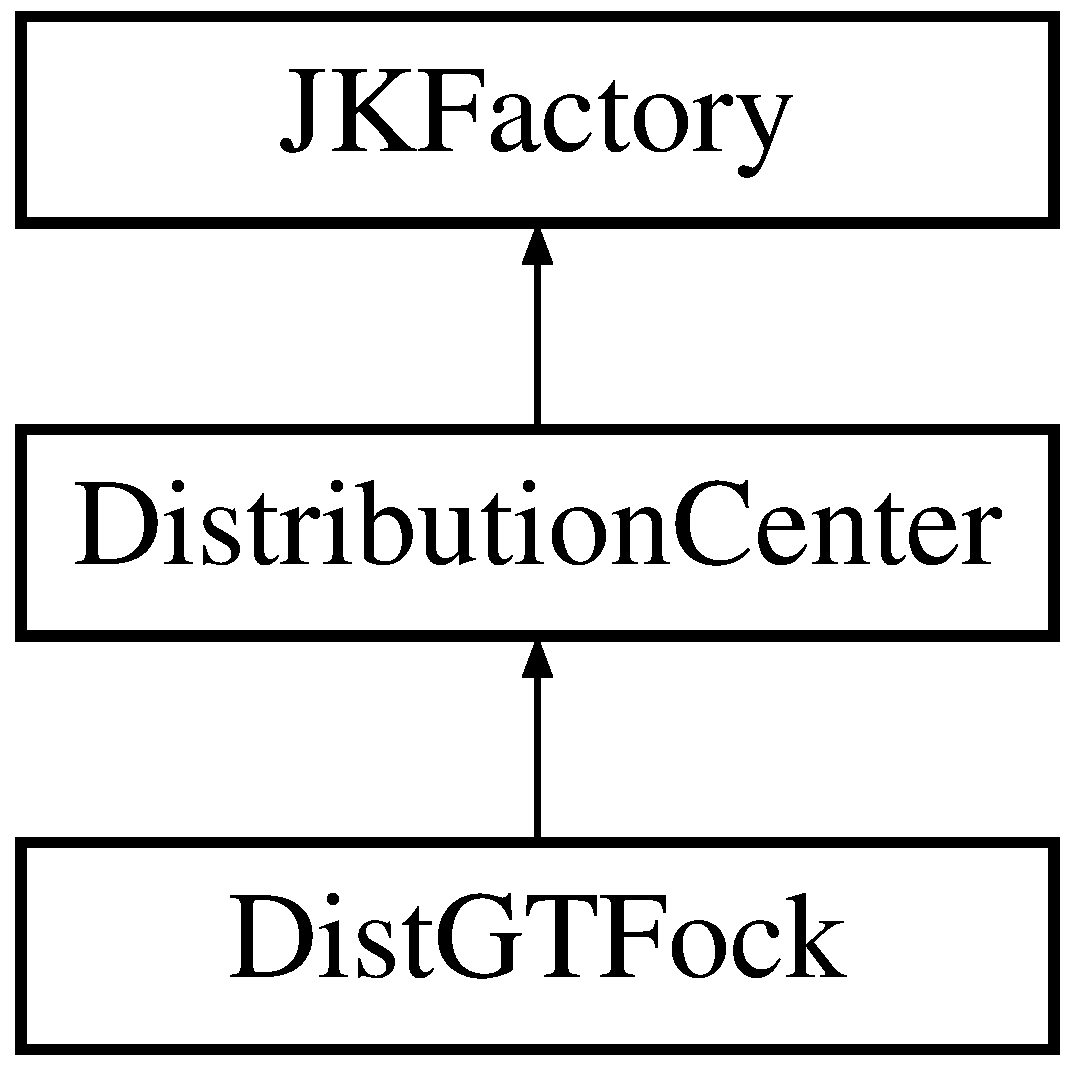
\includegraphics[height=3cm]{classJKBuilder_1_1DistributionCenter}
\end{center}
\end{figure}
\subsection*{Public Member Functions}
\begin{DoxyCompactItemize}
\item 
\hyperlink{classJKBuilder_1_1DistributionCenter_a188ebdd377e09a6e048a5e3f0b47a3ec}{DistributionCenter} (\hyperlink{classJKBuilder_1_1AOBasisSet}{AOBasisSet} $\ast$basis)
\begin{DoxyCompactList}\small\item\em Sets everything to NULL for the time being. \item\end{DoxyCompactList}\item 
virtual \hyperlink{classJKBuilder_1_1DistributionCenter_a2e0afd90ae098233a728d3c384196de2}{$\sim$DistributionCenter} ()
\begin{DoxyCompactList}\small\item\em Frees up memory associated with rho, J, and K. \item\end{DoxyCompactList}\item 
virtual void \hyperlink{classJKBuilder_1_1JKFactory_ae253b309dafe3ce003fdabfd315318b8}{BuildJK} (const double $\ast$DensityMatrix, \hyperlink{namespaceJKBuilder_aef21bc37b7cf7bc5ebb5a48628db8d0f}{SharedSymJKMatrix} \&J\_\-Matrix, \hyperlink{namespaceJKBuilder_aef21bc37b7cf7bc5ebb5a48628db8d0f}{SharedSymJKMatrix} \&K\_\-Matrix)=0
\begin{DoxyCompactList}\small\item\em The function actually in charge of building the J and K matrices. \item\end{DoxyCompactList}\end{DoxyCompactItemize}
\subsection*{Protected Attributes}
\begin{DoxyCompactItemize}
\item 
\hyperlink{classJKBuilder_1_1MPIManager}{MPIManager} $\ast$ \hyperlink{classJKBuilder_1_1DistributionCenter_a3753afd7c89e077643a274ed7c4e9129}{MPI}
\begin{DoxyCompactList}\small\item\em This is the object in charge of managing the parallelism. \item\end{DoxyCompactList}\item 
std::vector$<$ \hyperlink{namespaceJKBuilder_a3b337e72f5cb0686ec93e063dda09c70}{SharedDistMatrix} $>$ \hyperlink{classJKBuilder_1_1DistributionCenter_aea5bfaa6247d7c03edf480fa8ecdd929}{rho}
\begin{DoxyCompactList}\small\item\em The distributed density \hyperlink{classJKBuilder_1_1matrix}{matrix}. \item\end{DoxyCompactList}\item 
std::vector$<$ \hyperlink{namespaceJKBuilder_a3b337e72f5cb0686ec93e063dda09c70}{SharedDistMatrix} $>$ \hyperlink{classJKBuilder_1_1DistributionCenter_a83e7fc1320b7071187dce35322e659b2}{J}
\begin{DoxyCompactList}\small\item\em The distributed Coloumb \hyperlink{classJKBuilder_1_1matrix}{matrix}. \item\end{DoxyCompactList}\item 
std::vector$<$ \hyperlink{namespaceJKBuilder_a3b337e72f5cb0686ec93e063dda09c70}{SharedDistMatrix} $>$ \hyperlink{classJKBuilder_1_1DistributionCenter_a36d7716ac07910f43805622922c1fb93}{K}
\begin{DoxyCompactList}\small\item\em The distributed Exchange \hyperlink{classJKBuilder_1_1matrix}{matrix}. \item\end{DoxyCompactList}\end{DoxyCompactItemize}


\subsection{Detailed Description}
A distribution center is a \hyperlink{classJKBuilder_1_1JKFactory}{JKFactory} that makes distributed objects. The name distribution center is supposed to be a pun related to the name \char`\"{}factory\char`\"{}. It is a lame one, but I like it, so it stays. Either way, this is an abstract base class that actual Distributed routines derive from. For example the \hyperlink{namespaceGTFock}{GTFock} library is a derived class of this class. 

\subsection{Constructor \& Destructor Documentation}
\hypertarget{classJKBuilder_1_1DistributionCenter_a188ebdd377e09a6e048a5e3f0b47a3ec}{
\index{JKBuilder::DistributionCenter@{JKBuilder::DistributionCenter}!DistributionCenter@{DistributionCenter}}
\index{DistributionCenter@{DistributionCenter}!JKBuilder::DistributionCenter@{JKBuilder::DistributionCenter}}
\subsubsection[{DistributionCenter}]{\setlength{\rightskip}{0pt plus 5cm}{\bf DistributionCenter} ({\bf AOBasisSet} $\ast$ {\em basis})}}
\label{classJKBuilder_1_1DistributionCenter_a188ebdd377e09a6e048a5e3f0b47a3ec}


Sets everything to NULL for the time being. \hypertarget{classJKBuilder_1_1DistributionCenter_a2e0afd90ae098233a728d3c384196de2}{
\index{JKBuilder::DistributionCenter@{JKBuilder::DistributionCenter}!$\sim$DistributionCenter@{$\sim$DistributionCenter}}
\index{$\sim$DistributionCenter@{$\sim$DistributionCenter}!JKBuilder::DistributionCenter@{JKBuilder::DistributionCenter}}
\subsubsection[{$\sim$DistributionCenter}]{\setlength{\rightskip}{0pt plus 5cm}$\sim${\bf DistributionCenter} ()\hspace{0.3cm}{\ttfamily  \mbox{[}virtual\mbox{]}}}}
\label{classJKBuilder_1_1DistributionCenter_a2e0afd90ae098233a728d3c384196de2}


Frees up memory associated with rho, J, and K. 

\subsection{Member Function Documentation}
\hypertarget{classJKBuilder_1_1JKFactory_ae253b309dafe3ce003fdabfd315318b8}{
\index{JKBuilder::DistributionCenter@{JKBuilder::DistributionCenter}!BuildJK@{BuildJK}}
\index{BuildJK@{BuildJK}!JKBuilder::DistributionCenter@{JKBuilder::DistributionCenter}}
\subsubsection[{BuildJK}]{\setlength{\rightskip}{0pt plus 5cm}virtual void BuildJK (const double $\ast$ {\em DensityMatrix}, \/  {\bf SharedSymJKMatrix} \& {\em J\_\-Matrix}, \/  {\bf SharedSymJKMatrix} \& {\em K\_\-Matrix})\hspace{0.3cm}{\ttfamily  \mbox{[}pure virtual, inherited\mbox{]}}}}
\label{classJKBuilder_1_1JKFactory_ae253b309dafe3ce003fdabfd315318b8}


The function actually in charge of building the J and K matrices. This function first updates the density \hyperlink{classJKBuilder_1_1matrix}{matrix} to be the one given to it. Next, it computes J and K and returns them as \hyperlink{classJKBuilder_1_1matrix}{matrix} objects.


\begin{DoxyParams}{Parameters}
\item[\mbox{$\leftarrow$} {\em DensityMatrix}]The density \hyperlink{classJKBuilder_1_1matrix}{matrix} \item[\mbox{$\rightarrow$} {\em J}]The Coulomb \hyperlink{classJKBuilder_1_1matrix}{matrix} corresponding to DensityMatrix \item[\mbox{$\rightarrow$} {\em K}]The Exchange \hyperlink{classJKBuilder_1_1matrix}{matrix} corresponding to DensityMatrix \end{DoxyParams}


Implemented in \hyperlink{classGTFock_1_1DistGTFock_aea85d0b3d84e8e52819e8a15201e078a}{DistGTFock}, and \hyperlink{classJKBuilder_1_1PsiShared_aa5f73a8109ec88464262262164feda1e}{PsiShared}.

\subsection{Member Data Documentation}
\hypertarget{classJKBuilder_1_1DistributionCenter_a3753afd7c89e077643a274ed7c4e9129}{
\index{JKBuilder::DistributionCenter@{JKBuilder::DistributionCenter}!MPI@{MPI}}
\index{MPI@{MPI}!JKBuilder::DistributionCenter@{JKBuilder::DistributionCenter}}
\subsubsection[{MPI}]{\setlength{\rightskip}{0pt plus 5cm}{\bf MPIManager}$\ast$ {\bf MPI}\hspace{0.3cm}{\ttfamily  \mbox{[}protected\mbox{]}}}}
\label{classJKBuilder_1_1DistributionCenter_a3753afd7c89e077643a274ed7c4e9129}


This is the object in charge of managing the parallelism. \hypertarget{classJKBuilder_1_1DistributionCenter_aea5bfaa6247d7c03edf480fa8ecdd929}{
\index{JKBuilder::DistributionCenter@{JKBuilder::DistributionCenter}!rho@{rho}}
\index{rho@{rho}!JKBuilder::DistributionCenter@{JKBuilder::DistributionCenter}}
\subsubsection[{rho}]{\setlength{\rightskip}{0pt plus 5cm}std::vector$<${\bf SharedDistMatrix}$>$ {\bf rho}\hspace{0.3cm}{\ttfamily  \mbox{[}protected\mbox{]}}}}
\label{classJKBuilder_1_1DistributionCenter_aea5bfaa6247d7c03edf480fa8ecdd929}


The distributed density \hyperlink{classJKBuilder_1_1matrix}{matrix}. \hypertarget{classJKBuilder_1_1DistributionCenter_a83e7fc1320b7071187dce35322e659b2}{
\index{JKBuilder::DistributionCenter@{JKBuilder::DistributionCenter}!J@{J}}
\index{J@{J}!JKBuilder::DistributionCenter@{JKBuilder::DistributionCenter}}
\subsubsection[{J}]{\setlength{\rightskip}{0pt plus 5cm}std::vector$<${\bf SharedDistMatrix}$>$ {\bf J}\hspace{0.3cm}{\ttfamily  \mbox{[}protected\mbox{]}}}}
\label{classJKBuilder_1_1DistributionCenter_a83e7fc1320b7071187dce35322e659b2}


The distributed Coloumb \hyperlink{classJKBuilder_1_1matrix}{matrix}. \hypertarget{classJKBuilder_1_1DistributionCenter_a36d7716ac07910f43805622922c1fb93}{
\index{JKBuilder::DistributionCenter@{JKBuilder::DistributionCenter}!K@{K}}
\index{K@{K}!JKBuilder::DistributionCenter@{JKBuilder::DistributionCenter}}
\subsubsection[{K}]{\setlength{\rightskip}{0pt plus 5cm}std::vector$<${\bf SharedDistMatrix}$>$ {\bf K}\hspace{0.3cm}{\ttfamily  \mbox{[}protected\mbox{]}}}}
\label{classJKBuilder_1_1DistributionCenter_a36d7716ac07910f43805622922c1fb93}


The distributed Exchange \hyperlink{classJKBuilder_1_1matrix}{matrix}. 

The documentation for this class was generated from the following files:\begin{DoxyCompactItemize}
\item 
src/\hyperlink{DistributionCenter_8h}{DistributionCenter.h}\item 
src/\hyperlink{DistributionCenter_8cpp}{DistributionCenter.cpp}\end{DoxyCompactItemize}

\hypertarget{classJKBuilder_1_1error}{
\section{error Class Reference}
\label{classJKBuilder_1_1error}\index{JKBuilder::error@{JKBuilder::error}}
}


This is my \hyperlink{classJKBuilder_1_1error}{error} class, kills the program when EoL is called.  


{\ttfamily \#include $<$JKBuilder.h$>$}Inheritance diagram for error::\begin{figure}[H]
\begin{center}
\leavevmode
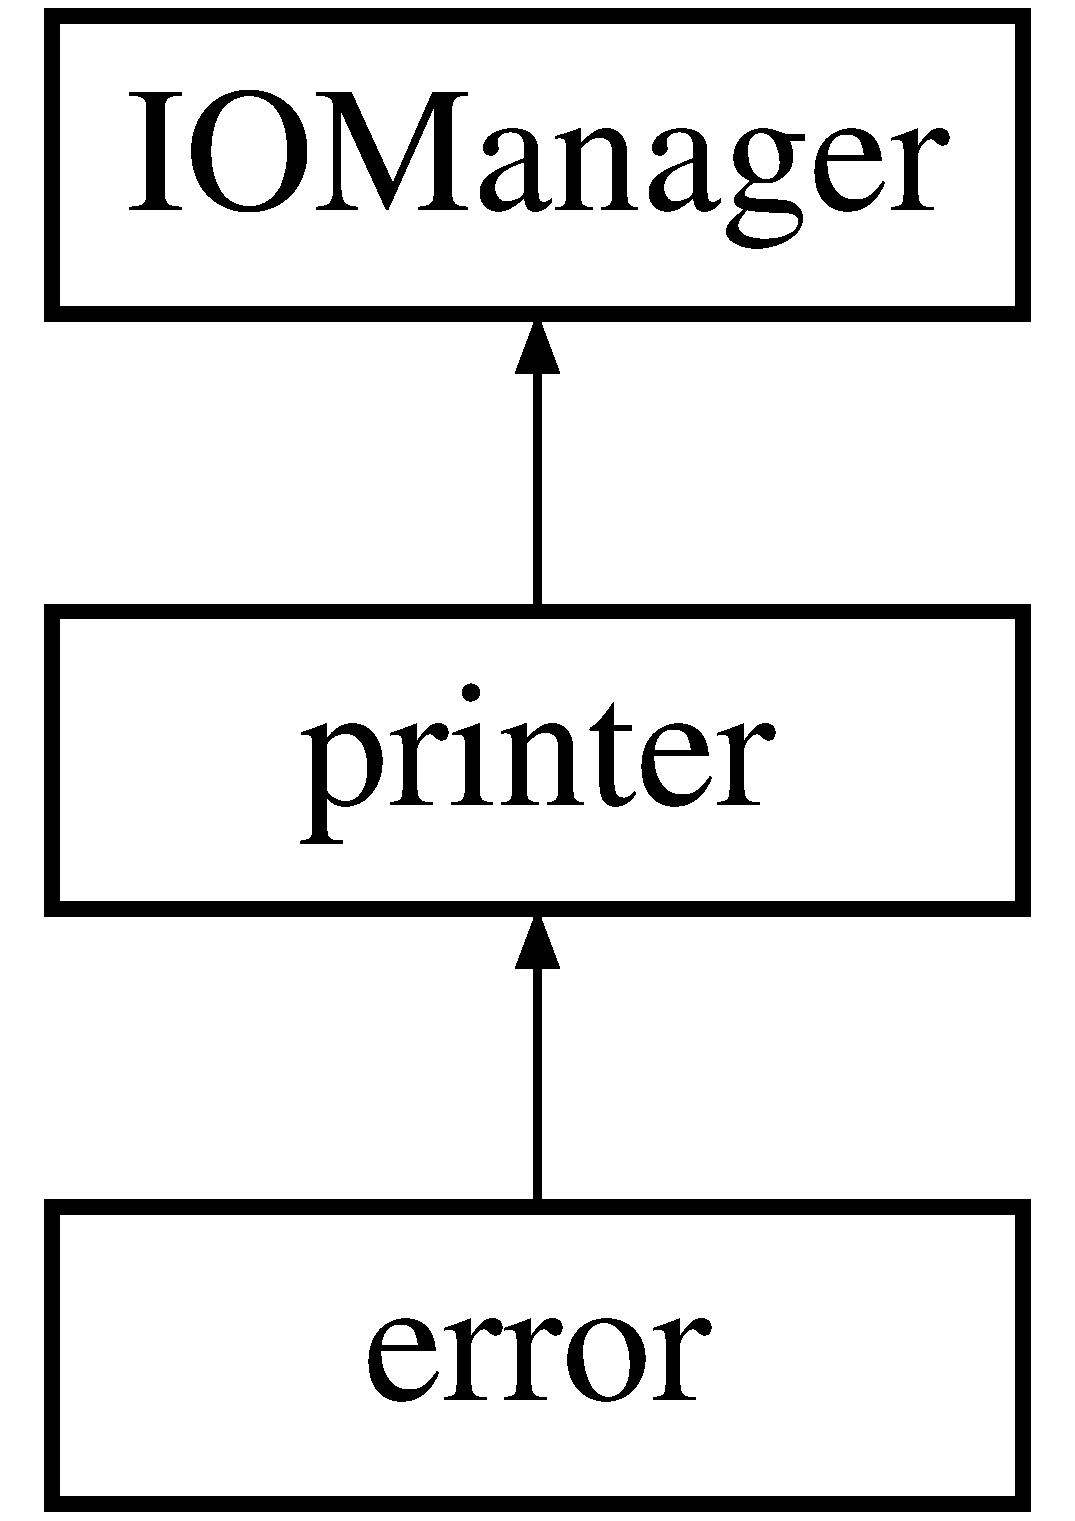
\includegraphics[height=3cm]{classJKBuilder_1_1error}
\end{center}
\end{figure}
\subsection*{Public Member Functions}
\begin{DoxyCompactItemize}
\item 
\hyperlink{classJKBuilder_1_1error_a43b8d30b879d4f09ceb059b02af2bc02}{error} ()
\item 
{\footnotesize template$<$class T $>$ }\\\hyperlink{classJKBuilder_1_1IOManager}{IOManager} \& \hyperlink{classJKBuilder_1_1IOManager_a505a35212a21e4884ed24b021c0add4b}{operator$<$$<$} (const T \&message)
\begin{DoxyCompactList}\small\item\em This is the call that prints our messages, unless it is a double... \item\end{DoxyCompactList}\item 
\hyperlink{classJKBuilder_1_1IOManager}{IOManager} \& \hyperlink{classJKBuilder_1_1IOManager_a127779d1803b6ffe9e44a3a36e46910e}{operator$<$$<$} (const double \&message)
\begin{DoxyCompactList}\small\item\em Then it is this call, because we want to control the precision then. \item\end{DoxyCompactList}\item 
\hyperlink{classJKBuilder_1_1IOManager}{IOManager} \& \hyperlink{classJKBuilder_1_1IOManager_a4ab394f377d37c6598659317320ec38c}{operator$<$$<$} (std::ostream \&($\ast$fn)(std::ostream \&))
\begin{DoxyCompactList}\small\item\em This function is used for the endl character. \item\end{DoxyCompactList}\end{DoxyCompactItemize}
\subsection*{Static Public Attributes}
\begin{DoxyCompactItemize}
\item 
static bool \hyperlink{classJKBuilder_1_1IOManager_aababa9aef0d20ddcfce2d78f41ae1dd8}{power} = true
\begin{DoxyCompactList}\small\item\em The state of the printer's power. \item\end{DoxyCompactList}\end{DoxyCompactItemize}
\subsection*{Protected Member Functions}
\begin{DoxyCompactItemize}
\item 
void \hyperlink{classJKBuilder_1_1error_a7f207ac705d33a0cd9794a9f0b4a1fa0}{EoL} ()
\begin{DoxyCompactList}\small\item\em This call kills the program, so only send endl, when you are done with the \hyperlink{classJKBuilder_1_1error}{error} message. \item\end{DoxyCompactList}\item 
void \hyperlink{classJKBuilder_1_1printer_aa32ee0a81ade611982bfc9861c5a05bb}{print} (const string message)
\begin{DoxyCompactList}\small\item\em This is the function that actually does the printing. \item\end{DoxyCompactList}\end{DoxyCompactItemize}
\subsection*{Protected Attributes}
\begin{DoxyCompactItemize}
\item 
std::stringstream \hyperlink{classJKBuilder_1_1IOManager_adbf6a7492c6521b38c1510aebe307770}{buffer}
\begin{DoxyCompactList}\small\item\em This is the line/data we want to print out. \item\end{DoxyCompactList}\item 
std::ostream $\ast$ \hyperlink{classJKBuilder_1_1IOManager_aafe3b1218427d92a689d147f74e74f4b}{Output}
\begin{DoxyCompactList}\small\item\em Returns the current output, defaults to cout. \item\end{DoxyCompactList}\item 
int \hyperlink{classJKBuilder_1_1IOManager_aa95455ed52a8459fad69509a4a0411b5}{precision}
\begin{DoxyCompactList}\small\item\em The precision a double will be printed to. \item\end{DoxyCompactList}\end{DoxyCompactItemize}


\subsection{Detailed Description}
This is my \hyperlink{classJKBuilder_1_1error}{error} class, kills the program when EoL is called. 

\subsection{Constructor \& Destructor Documentation}
\hypertarget{classJKBuilder_1_1error_a43b8d30b879d4f09ceb059b02af2bc02}{
\index{JKBuilder::error@{JKBuilder::error}!error@{error}}
\index{error@{error}!JKBuilder::error@{JKBuilder::error}}
\subsubsection[{error}]{\setlength{\rightskip}{0pt plus 5cm}{\bf error} ()}}
\label{classJKBuilder_1_1error_a43b8d30b879d4f09ceb059b02af2bc02}


\subsection{Member Function Documentation}
\hypertarget{classJKBuilder_1_1error_a7f207ac705d33a0cd9794a9f0b4a1fa0}{
\index{JKBuilder::error@{JKBuilder::error}!EoL@{EoL}}
\index{EoL@{EoL}!JKBuilder::error@{JKBuilder::error}}
\subsubsection[{EoL}]{\setlength{\rightskip}{0pt plus 5cm}void EoL ()\hspace{0.3cm}{\ttfamily  \mbox{[}protected, virtual\mbox{]}}}}
\label{classJKBuilder_1_1error_a7f207ac705d33a0cd9794a9f0b4a1fa0}


This call kills the program, so only send endl, when you are done with the \hyperlink{classJKBuilder_1_1error}{error} message. 

Reimplemented from \hyperlink{classJKBuilder_1_1printer_a7f207ac705d33a0cd9794a9f0b4a1fa0}{printer}.\hypertarget{classJKBuilder_1_1printer_aa32ee0a81ade611982bfc9861c5a05bb}{
\index{JKBuilder::error@{JKBuilder::error}!print@{print}}
\index{print@{print}!JKBuilder::error@{JKBuilder::error}}
\subsubsection[{print}]{\setlength{\rightskip}{0pt plus 5cm}void print (const string {\em message})\hspace{0.3cm}{\ttfamily  \mbox{[}protected, virtual, inherited\mbox{]}}}}
\label{classJKBuilder_1_1printer_aa32ee0a81ade611982bfc9861c5a05bb}


This is the function that actually does the printing. 

Reimplemented from \hyperlink{classJKBuilder_1_1IOManager_a3abc9519dd5220ecb1154daa25f557fe}{IOManager}.\hypertarget{classJKBuilder_1_1IOManager_a505a35212a21e4884ed24b021c0add4b}{
\index{JKBuilder::error@{JKBuilder::error}!operator$<$$<$@{operator$<$$<$}}
\index{operator$<$$<$@{operator$<$$<$}!JKBuilder::error@{JKBuilder::error}}
\subsubsection[{operator$<$$<$}]{\setlength{\rightskip}{0pt plus 5cm}{\bf IOManager} \& operator$<$$<$ (const T \& {\em message})\hspace{0.3cm}{\ttfamily  \mbox{[}inline, inherited\mbox{]}}}}
\label{classJKBuilder_1_1IOManager_a505a35212a21e4884ed24b021c0add4b}


This is the call that prints our messages, unless it is a double... \hypertarget{classJKBuilder_1_1IOManager_a127779d1803b6ffe9e44a3a36e46910e}{
\index{JKBuilder::error@{JKBuilder::error}!operator$<$$<$@{operator$<$$<$}}
\index{operator$<$$<$@{operator$<$$<$}!JKBuilder::error@{JKBuilder::error}}
\subsubsection[{operator$<$$<$}]{\setlength{\rightskip}{0pt plus 5cm}{\bf IOManager} \& operator$<$$<$ (const double \& {\em message})\hspace{0.3cm}{\ttfamily  \mbox{[}inherited\mbox{]}}}}
\label{classJKBuilder_1_1IOManager_a127779d1803b6ffe9e44a3a36e46910e}


Then it is this call, because we want to control the precision then. \hypertarget{classJKBuilder_1_1IOManager_a4ab394f377d37c6598659317320ec38c}{
\index{JKBuilder::error@{JKBuilder::error}!operator$<$$<$@{operator$<$$<$}}
\index{operator$<$$<$@{operator$<$$<$}!JKBuilder::error@{JKBuilder::error}}
\subsubsection[{operator$<$$<$}]{\setlength{\rightskip}{0pt plus 5cm}{\bf IOManager} \& operator$<$$<$ (std::ostream \&($\ast$)(std::ostream \&) {\em fn})\hspace{0.3cm}{\ttfamily  \mbox{[}inherited\mbox{]}}}}
\label{classJKBuilder_1_1IOManager_a4ab394f377d37c6598659317320ec38c}


This function is used for the endl character. When invoked with \char`\"{}endl\char`\"{} prints the content of the stringstream and clears it. Supports multiple endl's in a stream. The weird function signature is due to the signature of endl. 

\subsection{Member Data Documentation}
\hypertarget{classJKBuilder_1_1IOManager_adbf6a7492c6521b38c1510aebe307770}{
\index{JKBuilder::error@{JKBuilder::error}!buffer@{buffer}}
\index{buffer@{buffer}!JKBuilder::error@{JKBuilder::error}}
\subsubsection[{buffer}]{\setlength{\rightskip}{0pt plus 5cm}std::stringstream {\bf buffer}\hspace{0.3cm}{\ttfamily  \mbox{[}protected, inherited\mbox{]}}}}
\label{classJKBuilder_1_1IOManager_adbf6a7492c6521b38c1510aebe307770}


This is the line/data we want to print out. \hypertarget{classJKBuilder_1_1IOManager_aafe3b1218427d92a689d147f74e74f4b}{
\index{JKBuilder::error@{JKBuilder::error}!Output@{Output}}
\index{Output@{Output}!JKBuilder::error@{JKBuilder::error}}
\subsubsection[{Output}]{\setlength{\rightskip}{0pt plus 5cm}std::ostream$\ast$ {\bf Output}\hspace{0.3cm}{\ttfamily  \mbox{[}protected, inherited\mbox{]}}}}
\label{classJKBuilder_1_1IOManager_aafe3b1218427d92a689d147f74e74f4b}


Returns the current output, defaults to cout. \hypertarget{classJKBuilder_1_1IOManager_aa95455ed52a8459fad69509a4a0411b5}{
\index{JKBuilder::error@{JKBuilder::error}!precision@{precision}}
\index{precision@{precision}!JKBuilder::error@{JKBuilder::error}}
\subsubsection[{precision}]{\setlength{\rightskip}{0pt plus 5cm}int {\bf precision}\hspace{0.3cm}{\ttfamily  \mbox{[}protected, inherited\mbox{]}}}}
\label{classJKBuilder_1_1IOManager_aa95455ed52a8459fad69509a4a0411b5}


The precision a double will be printed to. \hypertarget{classJKBuilder_1_1IOManager_aababa9aef0d20ddcfce2d78f41ae1dd8}{
\index{JKBuilder::error@{JKBuilder::error}!power@{power}}
\index{power@{power}!JKBuilder::error@{JKBuilder::error}}
\subsubsection[{power}]{\setlength{\rightskip}{0pt plus 5cm}bool {\bf power} = true\hspace{0.3cm}{\ttfamily  \mbox{[}static, inherited\mbox{]}}}}
\label{classJKBuilder_1_1IOManager_aababa9aef0d20ddcfce2d78f41ae1dd8}


The state of the printer's power. If true then we are printing data to the output. If false then we are not. Note the static keyword. Turning off power for one \hyperlink{classJKBuilder_1_1printer}{printer} turns off the power for all of them. You flipped the breaker if you will. 

The documentation for this class was generated from the following files:\begin{DoxyCompactItemize}
\item 
src/\hyperlink{JKBuilder_8h}{JKBuilder.h}\item 
src/\hyperlink{JKBuilder_8cpp}{JKBuilder.cpp}\end{DoxyCompactItemize}

\hypertarget{classJKBuilder_1_1FileManager}{
\section{FileManager Class Reference}
\label{classJKBuilder_1_1FileManager}\index{JKBuilder::FileManager@{JKBuilder::FileManager}}
}


{\ttfamily \#include $<$FileManager.h$>$}Inheritance diagram for FileManager::\begin{figure}[H]
\begin{center}
\leavevmode
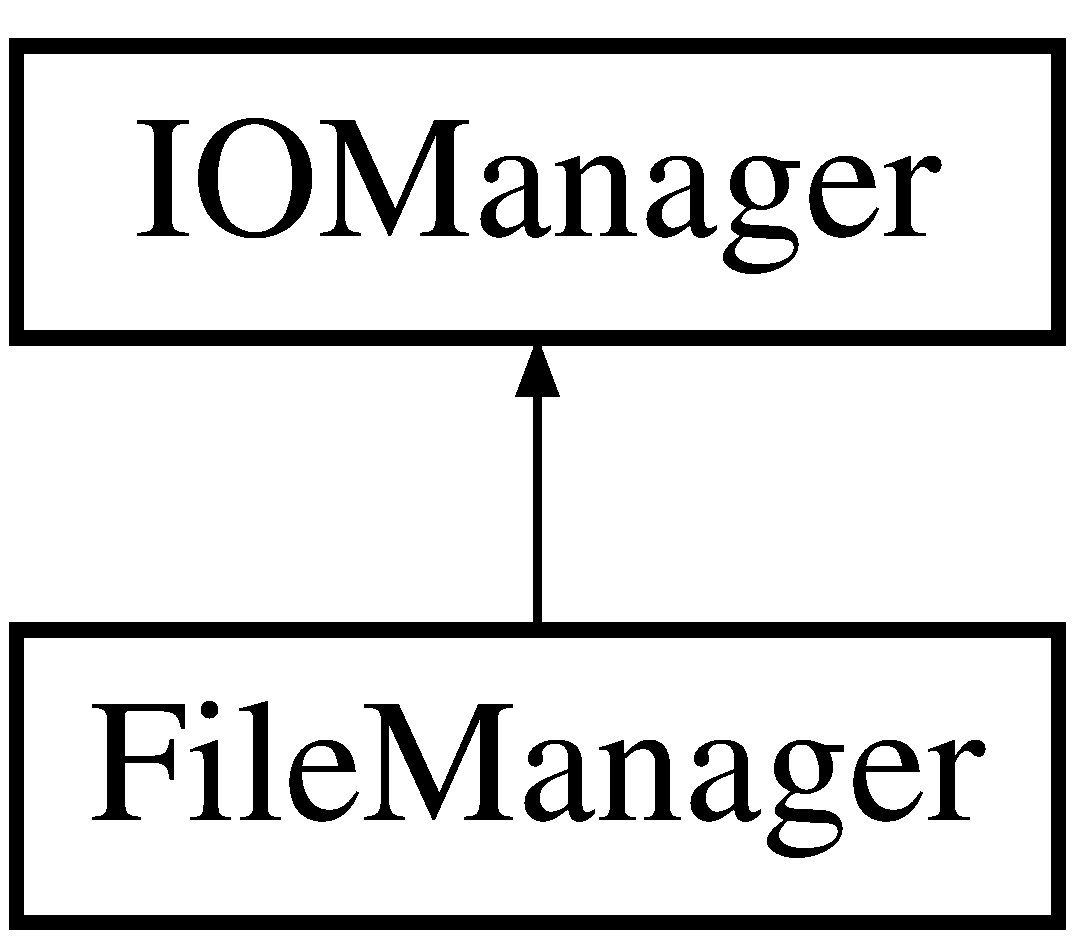
\includegraphics[height=2cm]{classJKBuilder_1_1FileManager}
\end{center}
\end{figure}
\subsection*{Public Member Functions}
\begin{DoxyCompactItemize}
\item 
void \hyperlink{classJKBuilder_1_1FileManager_a7f7a3199c392465d0767c6506c1af5b4}{Close} ()
\begin{DoxyCompactList}\small\item\em Will let the user close the file. \item\end{DoxyCompactList}\item 
\hyperlink{classJKBuilder_1_1FileManager_ad2b836abb993359aa5ee2cdaaf647a7f}{FileManager} (std::string filename)
\begin{DoxyCompactList}\small\item\em Defaults to mode =write. \item\end{DoxyCompactList}\item 
\hyperlink{classJKBuilder_1_1FileManager_acb45faebe31bb3a16cf5bf9e031a8f08}{$\sim$FileManager} ()
\begin{DoxyCompactList}\small\item\em Frees memory associated with the path and the file. \item\end{DoxyCompactList}\item 
{\footnotesize template$<$class T $>$ }\\\hyperlink{classJKBuilder_1_1IOManager}{IOManager} \& \hyperlink{classJKBuilder_1_1IOManager_a505a35212a21e4884ed24b021c0add4b}{operator$<$$<$} (const T \&message)
\begin{DoxyCompactList}\small\item\em This is the call that prints our messages, unless it is a double... \item\end{DoxyCompactList}\item 
\hyperlink{classJKBuilder_1_1IOManager}{IOManager} \& \hyperlink{classJKBuilder_1_1IOManager_a127779d1803b6ffe9e44a3a36e46910e}{operator$<$$<$} (const double \&message)
\begin{DoxyCompactList}\small\item\em Then it is this call, because we want to control the precision then. \item\end{DoxyCompactList}\item 
\hyperlink{classJKBuilder_1_1IOManager}{IOManager} \& \hyperlink{classJKBuilder_1_1IOManager_a4ab394f377d37c6598659317320ec38c}{operator$<$$<$} (std::ostream \&($\ast$fn)(std::ostream \&))
\begin{DoxyCompactList}\small\item\em This function is used for the endl character. \item\end{DoxyCompactList}\end{DoxyCompactItemize}
\subsection*{Static Public Attributes}
\begin{DoxyCompactItemize}
\item 
static bool \hyperlink{classJKBuilder_1_1IOManager_aababa9aef0d20ddcfce2d78f41ae1dd8}{power} = true
\begin{DoxyCompactList}\small\item\em The state of the printer's power. \item\end{DoxyCompactList}\end{DoxyCompactItemize}
\subsection*{Protected Member Functions}
\begin{DoxyCompactItemize}
\item 
virtual void \hyperlink{classJKBuilder_1_1IOManager_a3abc9519dd5220ecb1154daa25f557fe}{print} (const std::string message)
\begin{DoxyCompactList}\small\item\em This is the function that actually does the printing. \item\end{DoxyCompactList}\item 
virtual void \hyperlink{classJKBuilder_1_1IOManager_a7f207ac705d33a0cd9794a9f0b4a1fa0}{EoL} ()
\begin{DoxyCompactList}\small\item\em This is the function that prints the \char`\"{}end of line\char`\"{} character. \item\end{DoxyCompactList}\end{DoxyCompactItemize}
\subsection*{Protected Attributes}
\begin{DoxyCompactItemize}
\item 
std::stringstream \hyperlink{classJKBuilder_1_1IOManager_adbf6a7492c6521b38c1510aebe307770}{buffer}
\begin{DoxyCompactList}\small\item\em This is the line/data we want to print out. \item\end{DoxyCompactList}\item 
std::ostream $\ast$ \hyperlink{classJKBuilder_1_1IOManager_aafe3b1218427d92a689d147f74e74f4b}{Output}
\begin{DoxyCompactList}\small\item\em Returns the current output, defaults to cout. \item\end{DoxyCompactList}\item 
int \hyperlink{classJKBuilder_1_1IOManager_aa95455ed52a8459fad69509a4a0411b5}{precision}
\begin{DoxyCompactList}\small\item\em The precision a double will be printed to. \item\end{DoxyCompactList}\end{DoxyCompactItemize}
\subsection*{Private Member Functions}
\begin{DoxyCompactItemize}
\item 
void \hyperlink{classJKBuilder_1_1FileManager_a5e53001785ff30ae485a113b9b8a0ddc}{Open} ()
\begin{DoxyCompactList}\small\item\em Opens the file. \item\end{DoxyCompactList}\item 
bool \hyperlink{classJKBuilder_1_1FileManager_aa9a207f89881ad3eeb418619bef880ed}{Exists} ()
\begin{DoxyCompactList}\small\item\em Returns true if the file exists. \item\end{DoxyCompactList}\item 
bool \hyperlink{classJKBuilder_1_1FileManager_a1822528b9d87e3897acff000f0ef4629}{IsOpen} ()
\begin{DoxyCompactList}\small\item\em Returns true if the file is open. \item\end{DoxyCompactList}\end{DoxyCompactItemize}
\subsection*{Private Attributes}
\begin{DoxyCompactItemize}
\item 
std::string \hyperlink{classJKBuilder_1_1FileManager_a6c71000b535e65812d96eee3386307c4}{mode}
\begin{DoxyCompactList}\small\item\em Can be either \char`\"{}READ\char`\"{} or \char`\"{}WRITE\char`\"{}. \item\end{DoxyCompactList}\item 
std::fstream $\ast$ \hyperlink{classJKBuilder_1_1FileManager_a48c4cd5efd7b8b98629f1cd343d977a5}{file}
\begin{DoxyCompactList}\small\item\em This is the actual file. \item\end{DoxyCompactList}\item 
boost::filesystem::path $\ast$ \hyperlink{classJKBuilder_1_1FileManager_ac00a0f5150a654e2c127753617a833c8}{p}
\begin{DoxyCompactList}\small\item\em This the path to the file. \item\end{DoxyCompactList}\end{DoxyCompactItemize}


\subsection{Constructor \& Destructor Documentation}
\hypertarget{classJKBuilder_1_1FileManager_ad2b836abb993359aa5ee2cdaaf647a7f}{
\index{JKBuilder::FileManager@{JKBuilder::FileManager}!FileManager@{FileManager}}
\index{FileManager@{FileManager}!JKBuilder::FileManager@{JKBuilder::FileManager}}
\subsubsection[{FileManager}]{\setlength{\rightskip}{0pt plus 5cm}{\bf FileManager} (std::string {\em filename})}}
\label{classJKBuilder_1_1FileManager_ad2b836abb993359aa5ee2cdaaf647a7f}


Defaults to mode =write. \hypertarget{classJKBuilder_1_1FileManager_acb45faebe31bb3a16cf5bf9e031a8f08}{
\index{JKBuilder::FileManager@{JKBuilder::FileManager}!$\sim$FileManager@{$\sim$FileManager}}
\index{$\sim$FileManager@{$\sim$FileManager}!JKBuilder::FileManager@{JKBuilder::FileManager}}
\subsubsection[{$\sim$FileManager}]{\setlength{\rightskip}{0pt plus 5cm}$\sim${\bf FileManager} ()}}
\label{classJKBuilder_1_1FileManager_acb45faebe31bb3a16cf5bf9e031a8f08}


Frees memory associated with the path and the file. 

\subsection{Member Function Documentation}
\hypertarget{classJKBuilder_1_1FileManager_a5e53001785ff30ae485a113b9b8a0ddc}{
\index{JKBuilder::FileManager@{JKBuilder::FileManager}!Open@{Open}}
\index{Open@{Open}!JKBuilder::FileManager@{JKBuilder::FileManager}}
\subsubsection[{Open}]{\setlength{\rightskip}{0pt plus 5cm}void Open ()\hspace{0.3cm}{\ttfamily  \mbox{[}private\mbox{]}}}}
\label{classJKBuilder_1_1FileManager_a5e53001785ff30ae485a113b9b8a0ddc}


Opens the file. \hypertarget{classJKBuilder_1_1FileManager_aa9a207f89881ad3eeb418619bef880ed}{
\index{JKBuilder::FileManager@{JKBuilder::FileManager}!Exists@{Exists}}
\index{Exists@{Exists}!JKBuilder::FileManager@{JKBuilder::FileManager}}
\subsubsection[{Exists}]{\setlength{\rightskip}{0pt plus 5cm}bool Exists ()\hspace{0.3cm}{\ttfamily  \mbox{[}private\mbox{]}}}}
\label{classJKBuilder_1_1FileManager_aa9a207f89881ad3eeb418619bef880ed}


Returns true if the file exists. \hypertarget{classJKBuilder_1_1FileManager_a1822528b9d87e3897acff000f0ef4629}{
\index{JKBuilder::FileManager@{JKBuilder::FileManager}!IsOpen@{IsOpen}}
\index{IsOpen@{IsOpen}!JKBuilder::FileManager@{JKBuilder::FileManager}}
\subsubsection[{IsOpen}]{\setlength{\rightskip}{0pt plus 5cm}bool IsOpen ()\hspace{0.3cm}{\ttfamily  \mbox{[}private\mbox{]}}}}
\label{classJKBuilder_1_1FileManager_a1822528b9d87e3897acff000f0ef4629}


Returns true if the file is open. \hypertarget{classJKBuilder_1_1FileManager_a7f7a3199c392465d0767c6506c1af5b4}{
\index{JKBuilder::FileManager@{JKBuilder::FileManager}!Close@{Close}}
\index{Close@{Close}!JKBuilder::FileManager@{JKBuilder::FileManager}}
\subsubsection[{Close}]{\setlength{\rightskip}{0pt plus 5cm}void Close ()}}
\label{classJKBuilder_1_1FileManager_a7f7a3199c392465d0767c6506c1af5b4}


Will let the user close the file. \hypertarget{classJKBuilder_1_1IOManager_a3abc9519dd5220ecb1154daa25f557fe}{
\index{JKBuilder::FileManager@{JKBuilder::FileManager}!print@{print}}
\index{print@{print}!JKBuilder::FileManager@{JKBuilder::FileManager}}
\subsubsection[{print}]{\setlength{\rightskip}{0pt plus 5cm}void print (const std::string {\em message})\hspace{0.3cm}{\ttfamily  \mbox{[}protected, virtual, inherited\mbox{]}}}}
\label{classJKBuilder_1_1IOManager_a3abc9519dd5220ecb1154daa25f557fe}


This is the function that actually does the printing. 

Reimplemented in \hyperlink{classJKBuilder_1_1printer_aa32ee0a81ade611982bfc9861c5a05bb}{printer}.\hypertarget{classJKBuilder_1_1IOManager_a7f207ac705d33a0cd9794a9f0b4a1fa0}{
\index{JKBuilder::FileManager@{JKBuilder::FileManager}!EoL@{EoL}}
\index{EoL@{EoL}!JKBuilder::FileManager@{JKBuilder::FileManager}}
\subsubsection[{EoL}]{\setlength{\rightskip}{0pt plus 5cm}void EoL ()\hspace{0.3cm}{\ttfamily  \mbox{[}protected, virtual, inherited\mbox{]}}}}
\label{classJKBuilder_1_1IOManager_a7f207ac705d33a0cd9794a9f0b4a1fa0}


This is the function that prints the \char`\"{}end of line\char`\"{} character. 

Reimplemented in \hyperlink{classJKBuilder_1_1error_a7f207ac705d33a0cd9794a9f0b4a1fa0}{error}, and \hyperlink{classJKBuilder_1_1printer_a7f207ac705d33a0cd9794a9f0b4a1fa0}{printer}.\hypertarget{classJKBuilder_1_1IOManager_a505a35212a21e4884ed24b021c0add4b}{
\index{JKBuilder::FileManager@{JKBuilder::FileManager}!operator$<$$<$@{operator$<$$<$}}
\index{operator$<$$<$@{operator$<$$<$}!JKBuilder::FileManager@{JKBuilder::FileManager}}
\subsubsection[{operator$<$$<$}]{\setlength{\rightskip}{0pt plus 5cm}{\bf IOManager} \& operator$<$$<$ (const T \& {\em message})\hspace{0.3cm}{\ttfamily  \mbox{[}inline, inherited\mbox{]}}}}
\label{classJKBuilder_1_1IOManager_a505a35212a21e4884ed24b021c0add4b}


This is the call that prints our messages, unless it is a double... \hypertarget{classJKBuilder_1_1IOManager_a127779d1803b6ffe9e44a3a36e46910e}{
\index{JKBuilder::FileManager@{JKBuilder::FileManager}!operator$<$$<$@{operator$<$$<$}}
\index{operator$<$$<$@{operator$<$$<$}!JKBuilder::FileManager@{JKBuilder::FileManager}}
\subsubsection[{operator$<$$<$}]{\setlength{\rightskip}{0pt plus 5cm}{\bf IOManager} \& operator$<$$<$ (const double \& {\em message})\hspace{0.3cm}{\ttfamily  \mbox{[}inherited\mbox{]}}}}
\label{classJKBuilder_1_1IOManager_a127779d1803b6ffe9e44a3a36e46910e}


Then it is this call, because we want to control the precision then. \hypertarget{classJKBuilder_1_1IOManager_a4ab394f377d37c6598659317320ec38c}{
\index{JKBuilder::FileManager@{JKBuilder::FileManager}!operator$<$$<$@{operator$<$$<$}}
\index{operator$<$$<$@{operator$<$$<$}!JKBuilder::FileManager@{JKBuilder::FileManager}}
\subsubsection[{operator$<$$<$}]{\setlength{\rightskip}{0pt plus 5cm}{\bf IOManager} \& operator$<$$<$ (std::ostream \&($\ast$)(std::ostream \&) {\em fn})\hspace{0.3cm}{\ttfamily  \mbox{[}inherited\mbox{]}}}}
\label{classJKBuilder_1_1IOManager_a4ab394f377d37c6598659317320ec38c}


This function is used for the endl character. When invoked with \char`\"{}endl\char`\"{} prints the content of the stringstream and clears it. Supports multiple endl's in a stream. The weird function signature is due to the signature of endl. 

\subsection{Member Data Documentation}
\hypertarget{classJKBuilder_1_1FileManager_a6c71000b535e65812d96eee3386307c4}{
\index{JKBuilder::FileManager@{JKBuilder::FileManager}!mode@{mode}}
\index{mode@{mode}!JKBuilder::FileManager@{JKBuilder::FileManager}}
\subsubsection[{mode}]{\setlength{\rightskip}{0pt plus 5cm}std::string {\bf mode}\hspace{0.3cm}{\ttfamily  \mbox{[}private\mbox{]}}}}
\label{classJKBuilder_1_1FileManager_a6c71000b535e65812d96eee3386307c4}


Can be either \char`\"{}READ\char`\"{} or \char`\"{}WRITE\char`\"{}. \hypertarget{classJKBuilder_1_1FileManager_a48c4cd5efd7b8b98629f1cd343d977a5}{
\index{JKBuilder::FileManager@{JKBuilder::FileManager}!file@{file}}
\index{file@{file}!JKBuilder::FileManager@{JKBuilder::FileManager}}
\subsubsection[{file}]{\setlength{\rightskip}{0pt plus 5cm}std::fstream$\ast$ {\bf file}\hspace{0.3cm}{\ttfamily  \mbox{[}private\mbox{]}}}}
\label{classJKBuilder_1_1FileManager_a48c4cd5efd7b8b98629f1cd343d977a5}


This is the actual file. \hypertarget{classJKBuilder_1_1FileManager_ac00a0f5150a654e2c127753617a833c8}{
\index{JKBuilder::FileManager@{JKBuilder::FileManager}!p@{p}}
\index{p@{p}!JKBuilder::FileManager@{JKBuilder::FileManager}}
\subsubsection[{p}]{\setlength{\rightskip}{0pt plus 5cm}boost::filesystem::path$\ast$ {\bf p}\hspace{0.3cm}{\ttfamily  \mbox{[}private\mbox{]}}}}
\label{classJKBuilder_1_1FileManager_ac00a0f5150a654e2c127753617a833c8}


This the path to the file. \hypertarget{classJKBuilder_1_1IOManager_adbf6a7492c6521b38c1510aebe307770}{
\index{JKBuilder::FileManager@{JKBuilder::FileManager}!buffer@{buffer}}
\index{buffer@{buffer}!JKBuilder::FileManager@{JKBuilder::FileManager}}
\subsubsection[{buffer}]{\setlength{\rightskip}{0pt plus 5cm}std::stringstream {\bf buffer}\hspace{0.3cm}{\ttfamily  \mbox{[}protected, inherited\mbox{]}}}}
\label{classJKBuilder_1_1IOManager_adbf6a7492c6521b38c1510aebe307770}


This is the line/data we want to print out. \hypertarget{classJKBuilder_1_1IOManager_aafe3b1218427d92a689d147f74e74f4b}{
\index{JKBuilder::FileManager@{JKBuilder::FileManager}!Output@{Output}}
\index{Output@{Output}!JKBuilder::FileManager@{JKBuilder::FileManager}}
\subsubsection[{Output}]{\setlength{\rightskip}{0pt plus 5cm}std::ostream$\ast$ {\bf Output}\hspace{0.3cm}{\ttfamily  \mbox{[}protected, inherited\mbox{]}}}}
\label{classJKBuilder_1_1IOManager_aafe3b1218427d92a689d147f74e74f4b}


Returns the current output, defaults to cout. \hypertarget{classJKBuilder_1_1IOManager_aa95455ed52a8459fad69509a4a0411b5}{
\index{JKBuilder::FileManager@{JKBuilder::FileManager}!precision@{precision}}
\index{precision@{precision}!JKBuilder::FileManager@{JKBuilder::FileManager}}
\subsubsection[{precision}]{\setlength{\rightskip}{0pt plus 5cm}int {\bf precision}\hspace{0.3cm}{\ttfamily  \mbox{[}protected, inherited\mbox{]}}}}
\label{classJKBuilder_1_1IOManager_aa95455ed52a8459fad69509a4a0411b5}


The precision a double will be printed to. \hypertarget{classJKBuilder_1_1IOManager_aababa9aef0d20ddcfce2d78f41ae1dd8}{
\index{JKBuilder::FileManager@{JKBuilder::FileManager}!power@{power}}
\index{power@{power}!JKBuilder::FileManager@{JKBuilder::FileManager}}
\subsubsection[{power}]{\setlength{\rightskip}{0pt plus 5cm}bool {\bf power} = true\hspace{0.3cm}{\ttfamily  \mbox{[}static, inherited\mbox{]}}}}
\label{classJKBuilder_1_1IOManager_aababa9aef0d20ddcfce2d78f41ae1dd8}


The state of the printer's power. If true then we are printing data to the output. If false then we are not. Note the static keyword. Turning off power for one \hyperlink{classJKBuilder_1_1printer}{printer} turns off the power for all of them. You flipped the breaker if you will. 

The documentation for this class was generated from the following files:\begin{DoxyCompactItemize}
\item 
src/\hyperlink{FileManager_8h}{FileManager.h}\item 
src/\hyperlink{FileManager_8cpp}{FileManager.cpp}\end{DoxyCompactItemize}

\hypertarget{classJKBuilder_1_1Integrals}{
\section{Integrals Class Reference}
\label{classJKBuilder_1_1Integrals}\index{JKBuilder::Integrals@{JKBuilder::Integrals}}
}


The \hyperlink{classJKBuilder_1_1Integrals}{Integrals} class is an API to the various integral packages that may be used.  


{\ttfamily \#include $<$Integrals.h$>$}\subsection*{Public Member Functions}
\begin{DoxyCompactItemize}
\item 
void \hyperlink{classJKBuilder_1_1Integrals_a192b23625f0ca29472adb24ea0167d04}{AddFxns} (\hyperlink{Integrals_8h_ac8a8046e90f302a56e8d49058926be33}{ComputeFxn} \&CF, \hyperlink{Integrals_8h_ab945cefec686042cf6ebb998aa068552}{BufferFxn} \&BF)
\item 
\hyperlink{classJKBuilder_1_1Integrals_ad62b2f3d89ff3b7777582513a89381f0}{Integrals} ()
\item 
int \hyperlink{classJKBuilder_1_1Integrals_ac5087342e58e3fd449a58e82ea7e4b9c}{ComputeShell} (int P, int Q, int R, int S, int thread=0)
\item 
const double $\ast$ \hyperlink{classJKBuilder_1_1Integrals_ad0720a0de5aa5cbe34ac5f4b80754ee7}{TheIntegrals} (int thread=0)
\end{DoxyCompactItemize}
\subsection*{Private Attributes}
\begin{DoxyCompactItemize}
\item 
std::vector$<$ \hyperlink{Integrals_8h_ac8a8046e90f302a56e8d49058926be33}{ComputeFxn} $>$ \hyperlink{classJKBuilder_1_1Integrals_a968679304a6d15dd63858873608113b5}{ComputeInts}
\item 
std::vector$<$ \hyperlink{Integrals_8h_ab945cefec686042cf6ebb998aa068552}{BufferFxn} $>$ \hyperlink{classJKBuilder_1_1Integrals_a877ca0c4fd4342f3d3ca7078e65fbfeb}{DaInts}
\end{DoxyCompactItemize}


\subsection{Detailed Description}
The \hyperlink{classJKBuilder_1_1Integrals}{Integrals} class is an API to the various integral packages that may be used. The \hyperlink{classJKBuilder_1_1Integrals}{Integrals} class really does two things: calls the appropriate compute function and provides a way of accessing the actual elements. This is all accomplished by fxn pointers, meaning it's ability to do these things will be as fast or slow as the functions it calls. 

\subsection{Constructor \& Destructor Documentation}
\hypertarget{classJKBuilder_1_1Integrals_ad62b2f3d89ff3b7777582513a89381f0}{
\index{JKBuilder::Integrals@{JKBuilder::Integrals}!Integrals@{Integrals}}
\index{Integrals@{Integrals}!JKBuilder::Integrals@{JKBuilder::Integrals}}
\subsubsection[{Integrals}]{\setlength{\rightskip}{0pt plus 5cm}{\bf Integrals} ()}}
\label{classJKBuilder_1_1Integrals_ad62b2f3d89ff3b7777582513a89381f0}


\subsection{Member Function Documentation}
\hypertarget{classJKBuilder_1_1Integrals_a192b23625f0ca29472adb24ea0167d04}{
\index{JKBuilder::Integrals@{JKBuilder::Integrals}!AddFxns@{AddFxns}}
\index{AddFxns@{AddFxns}!JKBuilder::Integrals@{JKBuilder::Integrals}}
\subsubsection[{AddFxns}]{\setlength{\rightskip}{0pt plus 5cm}void AddFxns ({\bf ComputeFxn} \& {\em CF}, \/  {\bf BufferFxn} \& {\em BF})}}
\label{classJKBuilder_1_1Integrals_a192b23625f0ca29472adb24ea0167d04}
\hypertarget{classJKBuilder_1_1Integrals_ac5087342e58e3fd449a58e82ea7e4b9c}{
\index{JKBuilder::Integrals@{JKBuilder::Integrals}!ComputeShell@{ComputeShell}}
\index{ComputeShell@{ComputeShell}!JKBuilder::Integrals@{JKBuilder::Integrals}}
\subsubsection[{ComputeShell}]{\setlength{\rightskip}{0pt plus 5cm}int ComputeShell (int {\em P}, \/  int {\em Q}, \/  int {\em R}, \/  int {\em S}, \/  int {\em thread} = {\ttfamily 0})}}
\label{classJKBuilder_1_1Integrals_ac5087342e58e3fd449a58e82ea7e4b9c}
\hypertarget{classJKBuilder_1_1Integrals_ad0720a0de5aa5cbe34ac5f4b80754ee7}{
\index{JKBuilder::Integrals@{JKBuilder::Integrals}!TheIntegrals@{TheIntegrals}}
\index{TheIntegrals@{TheIntegrals}!JKBuilder::Integrals@{JKBuilder::Integrals}}
\subsubsection[{TheIntegrals}]{\setlength{\rightskip}{0pt plus 5cm}const double $\ast$ TheIntegrals (int {\em thread} = {\ttfamily 0})}}
\label{classJKBuilder_1_1Integrals_ad0720a0de5aa5cbe34ac5f4b80754ee7}


\subsection{Member Data Documentation}
\hypertarget{classJKBuilder_1_1Integrals_a968679304a6d15dd63858873608113b5}{
\index{JKBuilder::Integrals@{JKBuilder::Integrals}!ComputeInts@{ComputeInts}}
\index{ComputeInts@{ComputeInts}!JKBuilder::Integrals@{JKBuilder::Integrals}}
\subsubsection[{ComputeInts}]{\setlength{\rightskip}{0pt plus 5cm}std::vector$<${\bf ComputeFxn}$>$ {\bf ComputeInts}\hspace{0.3cm}{\ttfamily  \mbox{[}private\mbox{]}}}}
\label{classJKBuilder_1_1Integrals_a968679304a6d15dd63858873608113b5}
\hypertarget{classJKBuilder_1_1Integrals_a877ca0c4fd4342f3d3ca7078e65fbfeb}{
\index{JKBuilder::Integrals@{JKBuilder::Integrals}!DaInts@{DaInts}}
\index{DaInts@{DaInts}!JKBuilder::Integrals@{JKBuilder::Integrals}}
\subsubsection[{DaInts}]{\setlength{\rightskip}{0pt plus 5cm}std::vector$<${\bf BufferFxn}$>$ {\bf DaInts}\hspace{0.3cm}{\ttfamily  \mbox{[}private\mbox{]}}}}
\label{classJKBuilder_1_1Integrals_a877ca0c4fd4342f3d3ca7078e65fbfeb}


The documentation for this class was generated from the following files:\begin{DoxyCompactItemize}
\item 
src/\hyperlink{Integrals_8h}{Integrals.h}\item 
src/\hyperlink{Integrals_8cpp}{Integrals.cpp}\end{DoxyCompactItemize}

\hypertarget{classJKBuilder_1_1IOManager}{
\section{IOManager Class Reference}
\label{classJKBuilder_1_1IOManager}\index{JKBuilder::IOManager@{JKBuilder::IOManager}}
}


The class that controls the input and output (streams) of this library.  


{\ttfamily \#include $<$IOManager.h$>$}Inheritance diagram for IOManager::\begin{figure}[H]
\begin{center}
\leavevmode
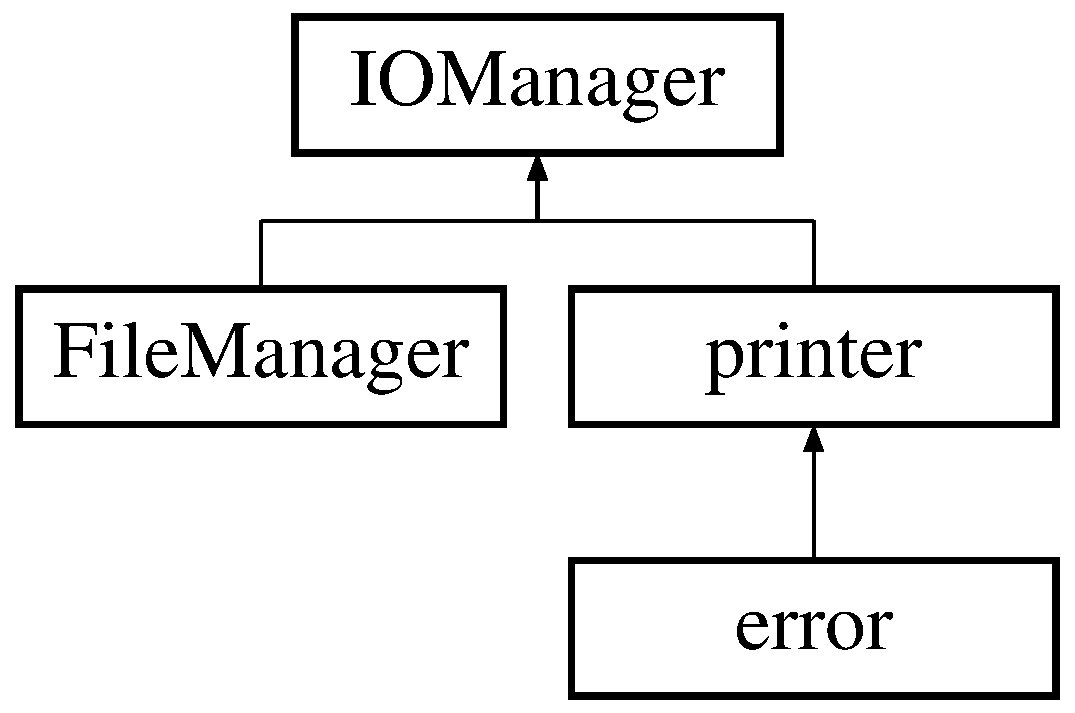
\includegraphics[height=3cm]{classJKBuilder_1_1IOManager}
\end{center}
\end{figure}
\subsection*{Public Member Functions}
\begin{DoxyCompactItemize}
\item 
{\footnotesize template$<$class T $>$ }\\\hyperlink{classJKBuilder_1_1IOManager}{IOManager} \& \hyperlink{classJKBuilder_1_1IOManager_a505a35212a21e4884ed24b021c0add4b}{operator$<$$<$} (const T \&message)
\begin{DoxyCompactList}\small\item\em This is the call that prints our messages, unless it is a double... \item\end{DoxyCompactList}\item 
\hyperlink{classJKBuilder_1_1IOManager}{IOManager} \& \hyperlink{classJKBuilder_1_1IOManager_a127779d1803b6ffe9e44a3a36e46910e}{operator$<$$<$} (const double \&message)
\begin{DoxyCompactList}\small\item\em Then it is this call, because we want to control the precision then. \item\end{DoxyCompactList}\item 
\hyperlink{classJKBuilder_1_1IOManager}{IOManager} \& \hyperlink{classJKBuilder_1_1IOManager_a4ab394f377d37c6598659317320ec38c}{operator$<$$<$} (std::ostream \&($\ast$fn)(std::ostream \&))
\begin{DoxyCompactList}\small\item\em This function is used for the endl character. \item\end{DoxyCompactList}\item 
\hyperlink{classJKBuilder_1_1IOManager_afabc1befb314e6ce3d793ab1319295c5}{IOManager} ()
\begin{DoxyCompactList}\small\item\em Defaults precision to 8 and Output=stdcout. \item\end{DoxyCompactList}\item 
virtual \hyperlink{classJKBuilder_1_1IOManager_ad7f67249558880cb6386ff44abea33f2}{$\sim$IOManager} ()
\begin{DoxyCompactList}\small\item\em No memory to free up so it does nothing. \item\end{DoxyCompactList}\end{DoxyCompactItemize}
\subsection*{Static Public Attributes}
\begin{DoxyCompactItemize}
\item 
static bool \hyperlink{classJKBuilder_1_1IOManager_aababa9aef0d20ddcfce2d78f41ae1dd8}{power} = true
\begin{DoxyCompactList}\small\item\em The state of the printer's power. \item\end{DoxyCompactList}\end{DoxyCompactItemize}
\subsection*{Protected Member Functions}
\begin{DoxyCompactItemize}
\item 
virtual void \hyperlink{classJKBuilder_1_1IOManager_a3abc9519dd5220ecb1154daa25f557fe}{print} (const std::string message)
\begin{DoxyCompactList}\small\item\em This is the function that actually does the printing. \item\end{DoxyCompactList}\item 
virtual void \hyperlink{classJKBuilder_1_1IOManager_a7f207ac705d33a0cd9794a9f0b4a1fa0}{EoL} ()
\begin{DoxyCompactList}\small\item\em This is the function that prints the \char`\"{}end of line\char`\"{} character. \item\end{DoxyCompactList}\end{DoxyCompactItemize}
\subsection*{Protected Attributes}
\begin{DoxyCompactItemize}
\item 
std::stringstream \hyperlink{classJKBuilder_1_1IOManager_adbf6a7492c6521b38c1510aebe307770}{buffer}
\begin{DoxyCompactList}\small\item\em This is the line/data we want to print out. \item\end{DoxyCompactList}\item 
std::ostream $\ast$ \hyperlink{classJKBuilder_1_1IOManager_aafe3b1218427d92a689d147f74e74f4b}{Output}
\begin{DoxyCompactList}\small\item\em Returns the current output, defaults to cout. \item\end{DoxyCompactList}\item 
int \hyperlink{classJKBuilder_1_1IOManager_aa95455ed52a8459fad69509a4a0411b5}{precision}
\begin{DoxyCompactList}\small\item\em The precision a double will be printed to. \item\end{DoxyCompactList}\end{DoxyCompactItemize}


\subsection{Detailed Description}
The class that controls the input and output (streams) of this library. For right now we are primarily interested in output, but support for input may be added later, in which case it makes sense to derive a IManager and an OManager 

\subsection{Constructor \& Destructor Documentation}
\hypertarget{classJKBuilder_1_1IOManager_afabc1befb314e6ce3d793ab1319295c5}{
\index{JKBuilder::IOManager@{JKBuilder::IOManager}!IOManager@{IOManager}}
\index{IOManager@{IOManager}!JKBuilder::IOManager@{JKBuilder::IOManager}}
\subsubsection[{IOManager}]{\setlength{\rightskip}{0pt plus 5cm}{\bf IOManager} ()}}
\label{classJKBuilder_1_1IOManager_afabc1befb314e6ce3d793ab1319295c5}


Defaults precision to 8 and Output=stdcout. \hypertarget{classJKBuilder_1_1IOManager_ad7f67249558880cb6386ff44abea33f2}{
\index{JKBuilder::IOManager@{JKBuilder::IOManager}!$\sim$IOManager@{$\sim$IOManager}}
\index{$\sim$IOManager@{$\sim$IOManager}!JKBuilder::IOManager@{JKBuilder::IOManager}}
\subsubsection[{$\sim$IOManager}]{\setlength{\rightskip}{0pt plus 5cm}$\sim${\bf IOManager} ()\hspace{0.3cm}{\ttfamily  \mbox{[}virtual\mbox{]}}}}
\label{classJKBuilder_1_1IOManager_ad7f67249558880cb6386ff44abea33f2}


No memory to free up so it does nothing. 

\subsection{Member Function Documentation}
\hypertarget{classJKBuilder_1_1IOManager_a3abc9519dd5220ecb1154daa25f557fe}{
\index{JKBuilder::IOManager@{JKBuilder::IOManager}!print@{print}}
\index{print@{print}!JKBuilder::IOManager@{JKBuilder::IOManager}}
\subsubsection[{print}]{\setlength{\rightskip}{0pt plus 5cm}void print (const std::string {\em message})\hspace{0.3cm}{\ttfamily  \mbox{[}protected, virtual\mbox{]}}}}
\label{classJKBuilder_1_1IOManager_a3abc9519dd5220ecb1154daa25f557fe}


This is the function that actually does the printing. 

Reimplemented in \hyperlink{classJKBuilder_1_1printer_aa32ee0a81ade611982bfc9861c5a05bb}{printer}.\hypertarget{classJKBuilder_1_1IOManager_a7f207ac705d33a0cd9794a9f0b4a1fa0}{
\index{JKBuilder::IOManager@{JKBuilder::IOManager}!EoL@{EoL}}
\index{EoL@{EoL}!JKBuilder::IOManager@{JKBuilder::IOManager}}
\subsubsection[{EoL}]{\setlength{\rightskip}{0pt plus 5cm}void EoL ()\hspace{0.3cm}{\ttfamily  \mbox{[}protected, virtual\mbox{]}}}}
\label{classJKBuilder_1_1IOManager_a7f207ac705d33a0cd9794a9f0b4a1fa0}


This is the function that prints the \char`\"{}end of line\char`\"{} character. 

Reimplemented in \hyperlink{classJKBuilder_1_1error_a7f207ac705d33a0cd9794a9f0b4a1fa0}{error}, and \hyperlink{classJKBuilder_1_1printer_a7f207ac705d33a0cd9794a9f0b4a1fa0}{printer}.\hypertarget{classJKBuilder_1_1IOManager_a505a35212a21e4884ed24b021c0add4b}{
\index{JKBuilder::IOManager@{JKBuilder::IOManager}!operator$<$$<$@{operator$<$$<$}}
\index{operator$<$$<$@{operator$<$$<$}!JKBuilder::IOManager@{JKBuilder::IOManager}}
\subsubsection[{operator$<$$<$}]{\setlength{\rightskip}{0pt plus 5cm}{\bf IOManager} \& operator$<$$<$ (const T \& {\em message})\hspace{0.3cm}{\ttfamily  \mbox{[}inline\mbox{]}}}}
\label{classJKBuilder_1_1IOManager_a505a35212a21e4884ed24b021c0add4b}


This is the call that prints our messages, unless it is a double... \hypertarget{classJKBuilder_1_1IOManager_a127779d1803b6ffe9e44a3a36e46910e}{
\index{JKBuilder::IOManager@{JKBuilder::IOManager}!operator$<$$<$@{operator$<$$<$}}
\index{operator$<$$<$@{operator$<$$<$}!JKBuilder::IOManager@{JKBuilder::IOManager}}
\subsubsection[{operator$<$$<$}]{\setlength{\rightskip}{0pt plus 5cm}{\bf IOManager} \& operator$<$$<$ (const double \& {\em message})}}
\label{classJKBuilder_1_1IOManager_a127779d1803b6ffe9e44a3a36e46910e}


Then it is this call, because we want to control the precision then. \hypertarget{classJKBuilder_1_1IOManager_a4ab394f377d37c6598659317320ec38c}{
\index{JKBuilder::IOManager@{JKBuilder::IOManager}!operator$<$$<$@{operator$<$$<$}}
\index{operator$<$$<$@{operator$<$$<$}!JKBuilder::IOManager@{JKBuilder::IOManager}}
\subsubsection[{operator$<$$<$}]{\setlength{\rightskip}{0pt plus 5cm}{\bf IOManager} \& operator$<$$<$ (std::ostream \&($\ast$)(std::ostream \&) {\em fn})}}
\label{classJKBuilder_1_1IOManager_a4ab394f377d37c6598659317320ec38c}


This function is used for the endl character. When invoked with \char`\"{}endl\char`\"{} prints the content of the stringstream and clears it. Supports multiple endl's in a stream. The weird function signature is due to the signature of endl. 

\subsection{Member Data Documentation}
\hypertarget{classJKBuilder_1_1IOManager_adbf6a7492c6521b38c1510aebe307770}{
\index{JKBuilder::IOManager@{JKBuilder::IOManager}!buffer@{buffer}}
\index{buffer@{buffer}!JKBuilder::IOManager@{JKBuilder::IOManager}}
\subsubsection[{buffer}]{\setlength{\rightskip}{0pt plus 5cm}std::stringstream {\bf buffer}\hspace{0.3cm}{\ttfamily  \mbox{[}protected\mbox{]}}}}
\label{classJKBuilder_1_1IOManager_adbf6a7492c6521b38c1510aebe307770}


This is the line/data we want to print out. \hypertarget{classJKBuilder_1_1IOManager_aafe3b1218427d92a689d147f74e74f4b}{
\index{JKBuilder::IOManager@{JKBuilder::IOManager}!Output@{Output}}
\index{Output@{Output}!JKBuilder::IOManager@{JKBuilder::IOManager}}
\subsubsection[{Output}]{\setlength{\rightskip}{0pt plus 5cm}std::ostream$\ast$ {\bf Output}\hspace{0.3cm}{\ttfamily  \mbox{[}protected\mbox{]}}}}
\label{classJKBuilder_1_1IOManager_aafe3b1218427d92a689d147f74e74f4b}


Returns the current output, defaults to cout. \hypertarget{classJKBuilder_1_1IOManager_aa95455ed52a8459fad69509a4a0411b5}{
\index{JKBuilder::IOManager@{JKBuilder::IOManager}!precision@{precision}}
\index{precision@{precision}!JKBuilder::IOManager@{JKBuilder::IOManager}}
\subsubsection[{precision}]{\setlength{\rightskip}{0pt plus 5cm}int {\bf precision}\hspace{0.3cm}{\ttfamily  \mbox{[}protected\mbox{]}}}}
\label{classJKBuilder_1_1IOManager_aa95455ed52a8459fad69509a4a0411b5}


The precision a double will be printed to. \hypertarget{classJKBuilder_1_1IOManager_aababa9aef0d20ddcfce2d78f41ae1dd8}{
\index{JKBuilder::IOManager@{JKBuilder::IOManager}!power@{power}}
\index{power@{power}!JKBuilder::IOManager@{JKBuilder::IOManager}}
\subsubsection[{power}]{\setlength{\rightskip}{0pt plus 5cm}bool {\bf power} = true\hspace{0.3cm}{\ttfamily  \mbox{[}static\mbox{]}}}}
\label{classJKBuilder_1_1IOManager_aababa9aef0d20ddcfce2d78f41ae1dd8}


The state of the printer's power. If true then we are printing data to the output. If false then we are not. Note the static keyword. Turning off power for one \hyperlink{classJKBuilder_1_1printer}{printer} turns off the power for all of them. You flipped the breaker if you will. 

The documentation for this class was generated from the following files:\begin{DoxyCompactItemize}
\item 
src/\hyperlink{IOManager_8h}{IOManager.h}\item 
src/\hyperlink{IOManager_8cpp}{IOManager.cpp}\end{DoxyCompactItemize}

\hypertarget{classJKBuilder_1_1Iterator}{
\section{Iterator Class Reference}
\label{classJKBuilder_1_1Iterator}\index{JKBuilder::Iterator@{JKBuilder::Iterator}}
}


{\ttfamily \#include $<$Iterators.h$>$}Inheritance diagram for Iterator::\begin{figure}[H]
\begin{center}
\leavevmode
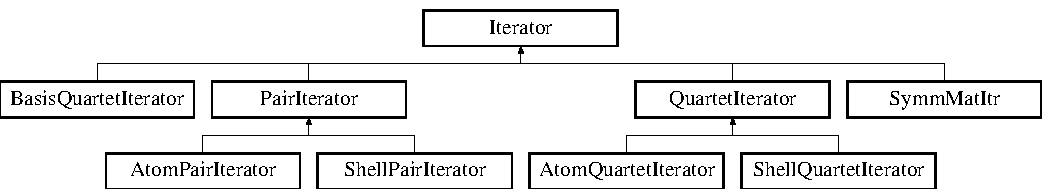
\includegraphics[height=2.54545cm]{classJKBuilder_1_1Iterator}
\end{center}
\end{figure}
\subsection*{Public Member Functions}
\begin{DoxyCompactItemize}
\item 
virtual void \hyperlink{classJKBuilder_1_1Iterator_a34ca36a99b20ae3170babadaffe51ed2}{Start} (int n=0)
\begin{DoxyCompactList}\small\item\em Returns an iterator suitable for starting on iteration n. \item\end{DoxyCompactList}\item 
virtual void \hyperlink{classJKBuilder_1_1Iterator_a5f692b73d2e160450f4617bb75825e11}{End} (int n=-\/1)
\begin{DoxyCompactList}\small\item\em Returns an iterator representing the state of the iterator after n iterations have occured. \item\end{DoxyCompactList}\item 
\hyperlink{classJKBuilder_1_1Iterator_a73347fde83464fe47afb15d2e34d86ad}{Iterator} (\hyperlink{classJKBuilder_1_1Iterator}{Iterator} const \&IteratorIn)
\item 
\hyperlink{classJKBuilder_1_1Iterator_a1f703720e1f5d97a0386c2dfe803c763}{Iterator} ()
\item 
virtual \hyperlink{classJKBuilder_1_1Iterator_a844b82815a73859e781b4798eb82f221}{$\sim$Iterator} ()
\item 
\hyperlink{classJKBuilder_1_1Iterator}{Iterator} \hyperlink{classJKBuilder_1_1Iterator_ac1702aedba13b4112b891b58dfd78eba}{operator++} (int)
\begin{DoxyCompactList}\small\item\em Increments the iterator after returning it's value. \item\end{DoxyCompactList}\item 
\hyperlink{classJKBuilder_1_1Iterator}{Iterator} \& \hyperlink{classJKBuilder_1_1Iterator_ae1f21c74128a5ef5d1b9de72ceb09be8}{operator++} ()
\begin{DoxyCompactList}\small\item\em Increments the iterator before returning it's value. \item\end{DoxyCompactList}\item 
bool \hyperlink{classJKBuilder_1_1Iterator_a1ea001976a5bc8ae8dc365e2a912b59a}{operator==} (const \hyperlink{classJKBuilder_1_1Iterator}{Iterator} \&other) const 
\item 
bool \hyperlink{classJKBuilder_1_1Iterator_a8c06af8ae0d9d1614ae9f81629275926}{operator!=} (const \hyperlink{classJKBuilder_1_1Iterator}{Iterator} \&other)
\begin{DoxyCompactList}\small\item\em Returns the opposite of operator==. \item\end{DoxyCompactList}\item 
\hyperlink{classJKBuilder_1_1Iterator}{Iterator} \& \hyperlink{classJKBuilder_1_1Iterator_ae6f4f24e1855d2aaf89a8a60a9f1521b}{operator=} (\hyperlink{classJKBuilder_1_1Iterator}{Iterator} const \&other)
\item 
void \hyperlink{classJKBuilder_1_1Iterator_aa83de505e29125c1d3ac7bb1b13ca15a}{SetStart} (std::vector$<$ int $>$ const \&other)
\begin{DoxyCompactList}\small\item\em Sets the N Indices to the N given in other. \item\end{DoxyCompactList}\item 
void \hyperlink{classJKBuilder_1_1Iterator_aad84ec668b5f41210db34c540aaa31fc}{SetEnd} (std::vector$<$ int $>$ const \&other)
\begin{DoxyCompactList}\small\item\em Sets the N MaxInd in other. \item\end{DoxyCompactList}\item 
int \hyperlink{classJKBuilder_1_1Iterator_a74247cf730a06b23fcb1ec64e5596b25}{operator\mbox{[}$\,$\mbox{]}} (const int i) const 
\begin{DoxyCompactList}\small\item\em Returns index i. \item\end{DoxyCompactList}\end{DoxyCompactItemize}
\subsection*{Protected Member Functions}
\begin{DoxyCompactItemize}
\item 
virtual void \hyperlink{classJKBuilder_1_1Iterator_a7874a07e98b52f4f147cde6f39353bae}{Iterate} ()
\end{DoxyCompactItemize}
\subsection*{Protected Attributes}
\begin{DoxyCompactItemize}
\item 
std::vector$<$ int $>$ \hyperlink{classJKBuilder_1_1Iterator_a20ca24f6d827aba144bb087c4bcb74a0}{CurrentValue}
\begin{DoxyCompactList}\small\item\em The current value. \item\end{DoxyCompactList}\item 
std::vector$<$ int $>$ \hyperlink{classJKBuilder_1_1Iterator_ab6b56d3c4e9353bc938dd6249cde9ca0}{MaxInd}
\begin{DoxyCompactList}\small\item\em This is a vector of length N containing the maximum each index can be. \item\end{DoxyCompactList}\end{DoxyCompactItemize}
\subsection*{Private Member Functions}
\begin{DoxyCompactItemize}
\item 
void \hyperlink{classJKBuilder_1_1Iterator_aacb7559eb1b8aab6e7bb6a56602d97ff}{Copy} (\hyperlink{classJKBuilder_1_1Iterator}{Iterator} const \&other)
\end{DoxyCompactItemize}


\subsection{Constructor \& Destructor Documentation}
\hypertarget{classJKBuilder_1_1Iterator_a73347fde83464fe47afb15d2e34d86ad}{
\index{JKBuilder::Iterator@{JKBuilder::Iterator}!Iterator@{Iterator}}
\index{Iterator@{Iterator}!JKBuilder::Iterator@{JKBuilder::Iterator}}
\subsubsection[{Iterator}]{\setlength{\rightskip}{0pt plus 5cm}{\bf Iterator} ({\bf Iterator} const \& {\em IteratorIn})}}
\label{classJKBuilder_1_1Iterator_a73347fde83464fe47afb15d2e34d86ad}
\hypertarget{classJKBuilder_1_1Iterator_a1f703720e1f5d97a0386c2dfe803c763}{
\index{JKBuilder::Iterator@{JKBuilder::Iterator}!Iterator@{Iterator}}
\index{Iterator@{Iterator}!JKBuilder::Iterator@{JKBuilder::Iterator}}
\subsubsection[{Iterator}]{\setlength{\rightskip}{0pt plus 5cm}{\bf Iterator} ()}}
\label{classJKBuilder_1_1Iterator_a1f703720e1f5d97a0386c2dfe803c763}
\hypertarget{classJKBuilder_1_1Iterator_a844b82815a73859e781b4798eb82f221}{
\index{JKBuilder::Iterator@{JKBuilder::Iterator}!$\sim$Iterator@{$\sim$Iterator}}
\index{$\sim$Iterator@{$\sim$Iterator}!JKBuilder::Iterator@{JKBuilder::Iterator}}
\subsubsection[{$\sim$Iterator}]{\setlength{\rightskip}{0pt plus 5cm}$\sim${\bf Iterator} ()\hspace{0.3cm}{\ttfamily  \mbox{[}virtual\mbox{]}}}}
\label{classJKBuilder_1_1Iterator_a844b82815a73859e781b4798eb82f221}


\subsection{Member Function Documentation}
\hypertarget{classJKBuilder_1_1Iterator_aacb7559eb1b8aab6e7bb6a56602d97ff}{
\index{JKBuilder::Iterator@{JKBuilder::Iterator}!Copy@{Copy}}
\index{Copy@{Copy}!JKBuilder::Iterator@{JKBuilder::Iterator}}
\subsubsection[{Copy}]{\setlength{\rightskip}{0pt plus 5cm}void Copy ({\bf Iterator} const \& {\em other})\hspace{0.3cm}{\ttfamily  \mbox{[}private\mbox{]}}}}
\label{classJKBuilder_1_1Iterator_aacb7559eb1b8aab6e7bb6a56602d97ff}


Reimplemented in \hyperlink{classJKBuilder_1_1PairIterator_ad9163efc0e961126baecc84da6555045}{PairIterator}, and \hyperlink{classJKBuilder_1_1QuartetIterator_a1cc9d53b063e002ead95abb45f05f0c3}{QuartetIterator}.\hypertarget{classJKBuilder_1_1Iterator_a7874a07e98b52f4f147cde6f39353bae}{
\index{JKBuilder::Iterator@{JKBuilder::Iterator}!Iterate@{Iterate}}
\index{Iterate@{Iterate}!JKBuilder::Iterator@{JKBuilder::Iterator}}
\subsubsection[{Iterate}]{\setlength{\rightskip}{0pt plus 5cm}void Iterate ()\hspace{0.3cm}{\ttfamily  \mbox{[}protected, virtual\mbox{]}}}}
\label{classJKBuilder_1_1Iterator_a7874a07e98b52f4f147cde6f39353bae}


Reimplemented in \hyperlink{classJKBuilder_1_1PairIterator_a7874a07e98b52f4f147cde6f39353bae}{PairIterator}, \hyperlink{classJKBuilder_1_1QuartetIterator_a7874a07e98b52f4f147cde6f39353bae}{QuartetIterator}, \hyperlink{classJKBuilder_1_1ShellPairIterator_a7874a07e98b52f4f147cde6f39353bae}{ShellPairIterator}, and \hyperlink{classJKBuilder_1_1SymmMatItr_a7874a07e98b52f4f147cde6f39353bae}{SymmMatItr}.\hypertarget{classJKBuilder_1_1Iterator_a34ca36a99b20ae3170babadaffe51ed2}{
\index{JKBuilder::Iterator@{JKBuilder::Iterator}!Start@{Start}}
\index{Start@{Start}!JKBuilder::Iterator@{JKBuilder::Iterator}}
\subsubsection[{Start}]{\setlength{\rightskip}{0pt plus 5cm}void Start (int {\em n} = {\ttfamily 0})\hspace{0.3cm}{\ttfamily  \mbox{[}virtual\mbox{]}}}}
\label{classJKBuilder_1_1Iterator_a34ca36a99b20ae3170babadaffe51ed2}


Returns an iterator suitable for starting on iteration n. 

Reimplemented in \hyperlink{classJKBuilder_1_1QuartetIterator_a34ca36a99b20ae3170babadaffe51ed2}{QuartetIterator}.\hypertarget{classJKBuilder_1_1Iterator_a5f692b73d2e160450f4617bb75825e11}{
\index{JKBuilder::Iterator@{JKBuilder::Iterator}!End@{End}}
\index{End@{End}!JKBuilder::Iterator@{JKBuilder::Iterator}}
\subsubsection[{End}]{\setlength{\rightskip}{0pt plus 5cm}void End (int {\em n} = {\ttfamily -\/1})\hspace{0.3cm}{\ttfamily  \mbox{[}virtual\mbox{]}}}}
\label{classJKBuilder_1_1Iterator_a5f692b73d2e160450f4617bb75825e11}


Returns an iterator representing the state of the iterator after n iterations have occured. The default argument is n=-\/1, which is a flag corresponding to the last iteration of the iterator 

Reimplemented in \hyperlink{classJKBuilder_1_1QuartetIterator_a5f692b73d2e160450f4617bb75825e11}{QuartetIterator}.\hypertarget{classJKBuilder_1_1Iterator_ac1702aedba13b4112b891b58dfd78eba}{
\index{JKBuilder::Iterator@{JKBuilder::Iterator}!operator++@{operator++}}
\index{operator++@{operator++}!JKBuilder::Iterator@{JKBuilder::Iterator}}
\subsubsection[{operator++}]{\setlength{\rightskip}{0pt plus 5cm}{\bf Iterator} operator++ (int)}}
\label{classJKBuilder_1_1Iterator_ac1702aedba13b4112b891b58dfd78eba}


Increments the iterator after returning it's value. \hypertarget{classJKBuilder_1_1Iterator_ae1f21c74128a5ef5d1b9de72ceb09be8}{
\index{JKBuilder::Iterator@{JKBuilder::Iterator}!operator++@{operator++}}
\index{operator++@{operator++}!JKBuilder::Iterator@{JKBuilder::Iterator}}
\subsubsection[{operator++}]{\setlength{\rightskip}{0pt plus 5cm}{\bf Iterator} \& operator++ ()}}
\label{classJKBuilder_1_1Iterator_ae1f21c74128a5ef5d1b9de72ceb09be8}


Increments the iterator before returning it's value. \hypertarget{classJKBuilder_1_1Iterator_a1ea001976a5bc8ae8dc365e2a912b59a}{
\index{JKBuilder::Iterator@{JKBuilder::Iterator}!operator==@{operator==}}
\index{operator==@{operator==}!JKBuilder::Iterator@{JKBuilder::Iterator}}
\subsubsection[{operator==}]{\setlength{\rightskip}{0pt plus 5cm}bool operator== (const {\bf Iterator} \& {\em other}) const}}
\label{classJKBuilder_1_1Iterator_a1ea001976a5bc8ae8dc365e2a912b59a}


Reimplemented in \hyperlink{classJKBuilder_1_1PairIterator_a6b4e430066f478e5e400edd39ef93968}{PairIterator}.\hypertarget{classJKBuilder_1_1Iterator_a8c06af8ae0d9d1614ae9f81629275926}{
\index{JKBuilder::Iterator@{JKBuilder::Iterator}!operator!=@{operator!=}}
\index{operator!=@{operator!=}!JKBuilder::Iterator@{JKBuilder::Iterator}}
\subsubsection[{operator!=}]{\setlength{\rightskip}{0pt plus 5cm}bool operator!= (const {\bf Iterator} \& {\em other})}}
\label{classJKBuilder_1_1Iterator_a8c06af8ae0d9d1614ae9f81629275926}


Returns the opposite of operator==. \hypertarget{classJKBuilder_1_1Iterator_ae6f4f24e1855d2aaf89a8a60a9f1521b}{
\index{JKBuilder::Iterator@{JKBuilder::Iterator}!operator=@{operator=}}
\index{operator=@{operator=}!JKBuilder::Iterator@{JKBuilder::Iterator}}
\subsubsection[{operator=}]{\setlength{\rightskip}{0pt plus 5cm}{\bf Iterator} \& operator= ({\bf Iterator} const \& {\em other})}}
\label{classJKBuilder_1_1Iterator_ae6f4f24e1855d2aaf89a8a60a9f1521b}


Reimplemented in \hyperlink{classJKBuilder_1_1PairIterator_a698aa7b3d6495bd74dcff5b93be868a8}{PairIterator}, \hyperlink{classJKBuilder_1_1QuartetIterator_ab3cd17222545586596dbbc6aa3ca7046}{QuartetIterator}, \hyperlink{classJKBuilder_1_1AtomPairIterator_aefda578091b26523e72740cec884aa45}{AtomPairIterator}, \hyperlink{classJKBuilder_1_1AtomQuartetIterator_a39f50a07009d2e9e81e1d64da594084f}{AtomQuartetIterator}, \hyperlink{classJKBuilder_1_1ShellPairIterator_af3001050bade3a939d83971d1a3f47e7}{ShellPairIterator}, and \hyperlink{classJKBuilder_1_1ShellQuartetIterator_acd8ac6ed2e831bcb87e65acc0de747db}{ShellQuartetIterator}.\hypertarget{classJKBuilder_1_1Iterator_aa83de505e29125c1d3ac7bb1b13ca15a}{
\index{JKBuilder::Iterator@{JKBuilder::Iterator}!SetStart@{SetStart}}
\index{SetStart@{SetStart}!JKBuilder::Iterator@{JKBuilder::Iterator}}
\subsubsection[{SetStart}]{\setlength{\rightskip}{0pt plus 5cm}void SetStart (std::vector$<$ int $>$ const \& {\em other})}}
\label{classJKBuilder_1_1Iterator_aa83de505e29125c1d3ac7bb1b13ca15a}


Sets the N Indices to the N given in other. \hypertarget{classJKBuilder_1_1Iterator_aad84ec668b5f41210db34c540aaa31fc}{
\index{JKBuilder::Iterator@{JKBuilder::Iterator}!SetEnd@{SetEnd}}
\index{SetEnd@{SetEnd}!JKBuilder::Iterator@{JKBuilder::Iterator}}
\subsubsection[{SetEnd}]{\setlength{\rightskip}{0pt plus 5cm}void SetEnd (std::vector$<$ int $>$ const \& {\em other})}}
\label{classJKBuilder_1_1Iterator_aad84ec668b5f41210db34c540aaa31fc}


Sets the N MaxInd in other. \hypertarget{classJKBuilder_1_1Iterator_a74247cf730a06b23fcb1ec64e5596b25}{
\index{JKBuilder::Iterator@{JKBuilder::Iterator}!operator\mbox{[}\mbox{]}@{operator[]}}
\index{operator\mbox{[}\mbox{]}@{operator[]}!JKBuilder::Iterator@{JKBuilder::Iterator}}
\subsubsection[{operator[]}]{\setlength{\rightskip}{0pt plus 5cm}int operator\mbox{[}$\,$\mbox{]} (const int {\em i}) const}}
\label{classJKBuilder_1_1Iterator_a74247cf730a06b23fcb1ec64e5596b25}


Returns index i. 

\subsection{Member Data Documentation}
\hypertarget{classJKBuilder_1_1Iterator_a20ca24f6d827aba144bb087c4bcb74a0}{
\index{JKBuilder::Iterator@{JKBuilder::Iterator}!CurrentValue@{CurrentValue}}
\index{CurrentValue@{CurrentValue}!JKBuilder::Iterator@{JKBuilder::Iterator}}
\subsubsection[{CurrentValue}]{\setlength{\rightskip}{0pt plus 5cm}std::vector$<$int$>$ {\bf CurrentValue}\hspace{0.3cm}{\ttfamily  \mbox{[}protected\mbox{]}}}}
\label{classJKBuilder_1_1Iterator_a20ca24f6d827aba144bb087c4bcb74a0}


The current value. \hypertarget{classJKBuilder_1_1Iterator_ab6b56d3c4e9353bc938dd6249cde9ca0}{
\index{JKBuilder::Iterator@{JKBuilder::Iterator}!MaxInd@{MaxInd}}
\index{MaxInd@{MaxInd}!JKBuilder::Iterator@{JKBuilder::Iterator}}
\subsubsection[{MaxInd}]{\setlength{\rightskip}{0pt plus 5cm}std::vector$<$int$>$ {\bf MaxInd}\hspace{0.3cm}{\ttfamily  \mbox{[}protected\mbox{]}}}}
\label{classJKBuilder_1_1Iterator_ab6b56d3c4e9353bc938dd6249cde9ca0}


This is a vector of length N containing the maximum each index can be. 

The documentation for this class was generated from the following files:\begin{DoxyCompactItemize}
\item 
src/\hyperlink{Iterators_8h}{Iterators.h}\item 
src/\hyperlink{Iterator_8cpp}{Iterator.cpp}\end{DoxyCompactItemize}

\hypertarget{classJKBuilder_1_1IteratorRules}{
\section{IteratorRules Class Reference}
\label{classJKBuilder_1_1IteratorRules}\index{JKBuilder::IteratorRules@{JKBuilder::IteratorRules}}
}


A set of rules governing how an iterator works.  


{\ttfamily \#include $<$IteratorRules.h$>$}\subsection*{Public Member Functions}
\begin{DoxyCompactItemize}
\item 
virtual bool \hyperlink{classJKBuilder_1_1IteratorRules_ae197a0b320460b5c5d42d58bc921ddbc}{IsAcceptable} (vector$<$ int $>$ \&Indices)
\begin{DoxyCompactList}\small\item\em Returns true if a set of indices. \item\end{DoxyCompactList}\item 
\hyperlink{classJKBuilder_1_1IteratorRules_ae657e753967d73a7b2966dccb364682b}{IteratorRules} ()
\item 
virtual \hyperlink{classJKBuilder_1_1IteratorRules_a59f6acedab9a2a18057b88a2c4d6df92}{$\sim$IteratorRules} ()
\end{DoxyCompactItemize}
\subsection*{Public Attributes}
\begin{DoxyCompactItemize}
\item 
vector$<$ int $>$ \hyperlink{classJKBuilder_1_1IteratorRules_a405a336c1e1fa1b3a7a3e906b07722bf}{FreshStart}
\begin{DoxyCompactList}\small\item\em This is the absolute first value an iterator playing by these rules can have. \item\end{DoxyCompactList}\item 
vector$<$ int $>$ \hyperlink{classJKBuilder_1_1IteratorRules_a1e9f42e2eb6c6f9752414b8e43a3b36a}{TotalEnd}
\begin{DoxyCompactList}\small\item\em This is the absolute last value an iterator playing by these rules can have. \item\end{DoxyCompactList}\end{DoxyCompactItemize}
\subsection*{Protected Attributes}
\begin{DoxyCompactItemize}
\item 
bool \hyperlink{classJKBuilder_1_1IteratorRules_afa98914b6f51cb9bd2eafa7c01a614e5}{LeftToRight}
\begin{DoxyCompactList}\small\item\em If true, we try increment the left most index that can be incremented, if false we start at the right. \item\end{DoxyCompactList}\item 
bool \hyperlink{classJKBuilder_1_1IteratorRules_a3cb2f931e32ad7450b106c2137dc5b7f}{Distinct}
\begin{DoxyCompactList}\small\item\em If true, then all indices must be different. \item\end{DoxyCompactList}\end{DoxyCompactItemize}


\subsection{Detailed Description}
A set of rules governing how an iterator works. One can envision several common ways one may want to increment 4 (chosen for the sake of argument) indices, all of which go up to n (again for the sake of argument):

0 0 0 0 0 0 0 1 0 0 0 2 ... 0 0 0 n 0 0 1 0 ... n n n n

or the left to right variant of this (mirror the lines above). Another common instance is incurred when we want to only count unique indices:

3 2 1 0 4 2 1 0 4 3 1 0 4 3 2 0 4 3 2 1 5 2 1 0 ... n n-\/1 n-\/2 n-\/3

the mirror case is again possible. 

\subsection{Constructor \& Destructor Documentation}
\hypertarget{classJKBuilder_1_1IteratorRules_ae657e753967d73a7b2966dccb364682b}{
\index{JKBuilder::IteratorRules@{JKBuilder::IteratorRules}!IteratorRules@{IteratorRules}}
\index{IteratorRules@{IteratorRules}!JKBuilder::IteratorRules@{JKBuilder::IteratorRules}}
\subsubsection[{IteratorRules}]{\setlength{\rightskip}{0pt plus 5cm}{\bf IteratorRules} ()}}
\label{classJKBuilder_1_1IteratorRules_ae657e753967d73a7b2966dccb364682b}
\hypertarget{classJKBuilder_1_1IteratorRules_a59f6acedab9a2a18057b88a2c4d6df92}{
\index{JKBuilder::IteratorRules@{JKBuilder::IteratorRules}!$\sim$IteratorRules@{$\sim$IteratorRules}}
\index{$\sim$IteratorRules@{$\sim$IteratorRules}!JKBuilder::IteratorRules@{JKBuilder::IteratorRules}}
\subsubsection[{$\sim$IteratorRules}]{\setlength{\rightskip}{0pt plus 5cm}$\sim${\bf IteratorRules} ()\hspace{0.3cm}{\ttfamily  \mbox{[}virtual\mbox{]}}}}
\label{classJKBuilder_1_1IteratorRules_a59f6acedab9a2a18057b88a2c4d6df92}


\subsection{Member Function Documentation}
\hypertarget{classJKBuilder_1_1IteratorRules_ae197a0b320460b5c5d42d58bc921ddbc}{
\index{JKBuilder::IteratorRules@{JKBuilder::IteratorRules}!IsAcceptable@{IsAcceptable}}
\index{IsAcceptable@{IsAcceptable}!JKBuilder::IteratorRules@{JKBuilder::IteratorRules}}
\subsubsection[{IsAcceptable}]{\setlength{\rightskip}{0pt plus 5cm}bool IsAcceptable (vector$<$ int $>$ \& {\em Indices})\hspace{0.3cm}{\ttfamily  \mbox{[}virtual\mbox{]}}}}
\label{classJKBuilder_1_1IteratorRules_ae197a0b320460b5c5d42d58bc921ddbc}


Returns true if a set of indices. 

\subsection{Member Data Documentation}
\hypertarget{classJKBuilder_1_1IteratorRules_afa98914b6f51cb9bd2eafa7c01a614e5}{
\index{JKBuilder::IteratorRules@{JKBuilder::IteratorRules}!LeftToRight@{LeftToRight}}
\index{LeftToRight@{LeftToRight}!JKBuilder::IteratorRules@{JKBuilder::IteratorRules}}
\subsubsection[{LeftToRight}]{\setlength{\rightskip}{0pt plus 5cm}bool {\bf LeftToRight}\hspace{0.3cm}{\ttfamily  \mbox{[}protected\mbox{]}}}}
\label{classJKBuilder_1_1IteratorRules_afa98914b6f51cb9bd2eafa7c01a614e5}


If true, we try increment the left most index that can be incremented, if false we start at the right. \hypertarget{classJKBuilder_1_1IteratorRules_a3cb2f931e32ad7450b106c2137dc5b7f}{
\index{JKBuilder::IteratorRules@{JKBuilder::IteratorRules}!Distinct@{Distinct}}
\index{Distinct@{Distinct}!JKBuilder::IteratorRules@{JKBuilder::IteratorRules}}
\subsubsection[{Distinct}]{\setlength{\rightskip}{0pt plus 5cm}bool {\bf Distinct}\hspace{0.3cm}{\ttfamily  \mbox{[}protected\mbox{]}}}}
\label{classJKBuilder_1_1IteratorRules_a3cb2f931e32ad7450b106c2137dc5b7f}


If true, then all indices must be different. \hypertarget{classJKBuilder_1_1IteratorRules_a405a336c1e1fa1b3a7a3e906b07722bf}{
\index{JKBuilder::IteratorRules@{JKBuilder::IteratorRules}!FreshStart@{FreshStart}}
\index{FreshStart@{FreshStart}!JKBuilder::IteratorRules@{JKBuilder::IteratorRules}}
\subsubsection[{FreshStart}]{\setlength{\rightskip}{0pt plus 5cm}vector$<$int$>$ {\bf FreshStart}}}
\label{classJKBuilder_1_1IteratorRules_a405a336c1e1fa1b3a7a3e906b07722bf}


This is the absolute first value an iterator playing by these rules can have. \hypertarget{classJKBuilder_1_1IteratorRules_a1e9f42e2eb6c6f9752414b8e43a3b36a}{
\index{JKBuilder::IteratorRules@{JKBuilder::IteratorRules}!TotalEnd@{TotalEnd}}
\index{TotalEnd@{TotalEnd}!JKBuilder::IteratorRules@{JKBuilder::IteratorRules}}
\subsubsection[{TotalEnd}]{\setlength{\rightskip}{0pt plus 5cm}vector$<$int$>$ {\bf TotalEnd}}}
\label{classJKBuilder_1_1IteratorRules_a1e9f42e2eb6c6f9752414b8e43a3b36a}


This is the absolute last value an iterator playing by these rules can have. 

The documentation for this class was generated from the following files:\begin{DoxyCompactItemize}
\item 
src/\hyperlink{IteratorRules_8h}{IteratorRules.h}\item 
src/\hyperlink{IteratorRules_8cpp}{IteratorRules.cpp}\end{DoxyCompactItemize}

\hypertarget{classJKBuilder_1_1JK}{
\section{JK Class Reference}
\label{classJKBuilder_1_1JK}\index{JKBuilder::JK@{JKBuilder::JK}}
}


The main API to the \hyperlink{classJKBuilder_1_1JK}{JK} Builder Library.  


{\ttfamily \#include $<$JK.h$>$}Inheritance diagram for JK::\begin{figure}[H]
\begin{center}
\leavevmode
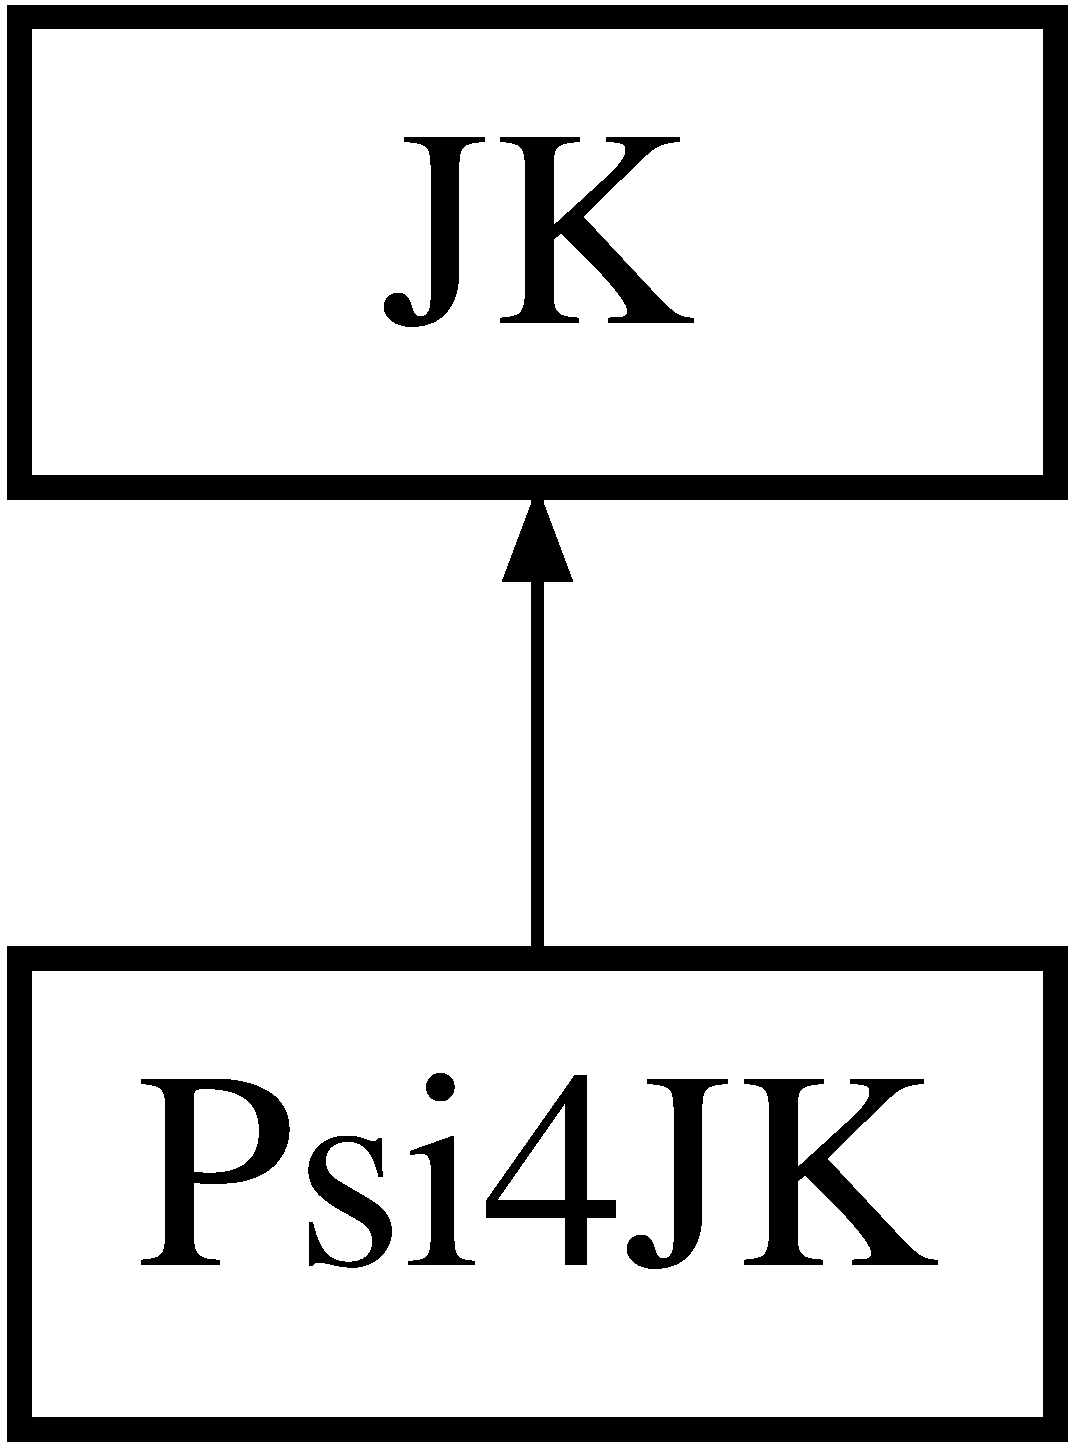
\includegraphics[height=2cm]{classJKBuilder_1_1JK}
\end{center}
\end{figure}
\subsection*{Public Member Functions}
\begin{DoxyCompactItemize}
\item 
void \hyperlink{classJKBuilder_1_1JK_ac0b62715458b98f8426017fdd8864670}{UpdateDensity} (const double $\ast$DensityMatrix)
\item 
double $\ast$ \hyperlink{classJKBuilder_1_1JK_ada0787d51feb1496d4aa3a786f870f88}{J\_\-Address} ()
\item 
double $\ast$ \hyperlink{classJKBuilder_1_1JK_a198d3c4da107eb0d9cfafa795f8d635b}{K\_\-Address} ()
\item 
double $\ast$ \hyperlink{classJKBuilder_1_1JK_a5104eb472d984f59df6ca3b91c625209}{Rho} ()
\item 
\hyperlink{classJKBuilder_1_1JK_ab667fd0f6ae1fdbf02a7aed8eb4cd4a8}{JK} ()
\item 
\hyperlink{classJKBuilder_1_1JK_a80533e1759361da2e871e53ba64161af}{$\sim$JK} ()
\begin{DoxyCompactList}\small\item\em Frees memory. \item\end{DoxyCompactList}\end{DoxyCompactItemize}
\subsection*{Protected Member Functions}
\begin{DoxyCompactItemize}
\item 
void \hyperlink{classJKBuilder_1_1JK_a13b685265e196c183897777ec2f3136a}{SetUp} (\hyperlink{classJKBuilder_1_1AOBasisSet}{AOBasisSet} $\ast$\hyperlink{classJKBuilder_1_1JK_a81392b84b45d3cf84c5c105e9fd5d09c}{basis}, \hyperlink{classJKBuilder_1_1molecule__class}{molecule\_\-class} $\ast$\hyperlink{classJKBuilder_1_1JK_ad646bdee4fc9f601f954b4a98c4da476}{molecule}, const double $\ast$DensityMatrix, double $\ast$\hyperlink{classJKBuilder_1_1JK_aa04a91cc219b5dabfce19d5316f96887}{J}, double $\ast$\hyperlink{classJKBuilder_1_1JK_a5160b673d25f0110d98097f8e7364315}{K})
\begin{DoxyCompactList}\small\item\em Sets up a bare-\/bones, distributed, \hyperlink{classJKBuilder_1_1JK}{JK} object in the DesiredBasis, on the desired molecule. \item\end{DoxyCompactList}\end{DoxyCompactItemize}
\subsection*{Protected Attributes}
\begin{DoxyCompactItemize}
\item 
bool \hyperlink{classJKBuilder_1_1JK_a072479da68be17a25570325316eade23}{Distributed}
\begin{DoxyCompactList}\small\item\em Are we calling the distributed \hyperlink{classJKBuilder_1_1JK}{JK} Builder, then true. False if we want the shared memory version. \item\end{DoxyCompactList}\item 
bool \hyperlink{classJKBuilder_1_1JK_a6324fcb7d27b80663a26f90a35f2e9b9}{Disk}
\begin{DoxyCompactList}\small\item\em Are we storing stuff on disk (true) or in memory (false). \item\end{DoxyCompactList}\item 
\hyperlink{classJKBuilder_1_1JKFactory}{JKFactory} $\ast$ \hyperlink{classJKBuilder_1_1JK_a09e4ffeb9ba2c95bf981da66beecc033}{SweatShop}
\begin{DoxyCompactList}\small\item\em Handles all the building of J and K objects. \item\end{DoxyCompactList}\item 
\hyperlink{classJKBuilder_1_1molecule__class}{molecule\_\-class} $\ast$ \hyperlink{classJKBuilder_1_1JK_ad646bdee4fc9f601f954b4a98c4da476}{molecule}
\item 
std::vector$<$ \hyperlink{namespaceJKBuilder_aef21bc37b7cf7bc5ebb5a48628db8d0f}{SharedSymJKMatrix} $>$ \hyperlink{classJKBuilder_1_1JK_aa04a91cc219b5dabfce19d5316f96887}{J}
\begin{DoxyCompactList}\small\item\em The J \hyperlink{classJKBuilder_1_1matrix}{matrix}. \item\end{DoxyCompactList}\item 
std::vector$<$ \hyperlink{namespaceJKBuilder_aef21bc37b7cf7bc5ebb5a48628db8d0f}{SharedSymJKMatrix} $>$ \hyperlink{classJKBuilder_1_1JK_a5160b673d25f0110d98097f8e7364315}{K}
\begin{DoxyCompactList}\small\item\em The K \hyperlink{classJKBuilder_1_1matrix}{matrix}. \item\end{DoxyCompactList}\item 
\hyperlink{classJKBuilder_1_1AOBasisSet}{AOBasisSet} $\ast$ \hyperlink{classJKBuilder_1_1JK_a81392b84b45d3cf84c5c105e9fd5d09c}{basis}
\item 
\hyperlink{classJKBuilder_1_1Integrals}{Integrals} \hyperlink{classJKBuilder_1_1JK_ad95ede2076c192d856848b3635efc38e}{DaInts}
\end{DoxyCompactItemize}


\subsection{Detailed Description}
The main API to the \hyperlink{classJKBuilder_1_1JK}{JK} Builder Library. The idea of the \hyperlink{classJKBuilder_1_1JK}{JK} Builder Library is to provide a nice, clean, easy to use way to build J and K matrices using distributed or shared architectures. This is to some extent the class that handles it (I say some extent because it is advisable and probably really good practice to derive from this class a child class that turns your objects into the input for my class, see Psi4JK for an example that turns Psi4's objects into my objects). If you are interfacing with my class your goal should be to call the SetUp function with the appropriate objects, which are the basis set, the molecule, the density \hyperlink{classJKBuilder_1_1matrix}{matrix}, the J \hyperlink{classJKBuilder_1_1matrix}{matrix}, and the K \hyperlink{classJKBuilder_1_1matrix}{matrix} (the last three are double stars for maximum compatibility) 

\subsection{Constructor \& Destructor Documentation}
\hypertarget{classJKBuilder_1_1JK_ab667fd0f6ae1fdbf02a7aed8eb4cd4a8}{
\index{JKBuilder::JK@{JKBuilder::JK}!JK@{JK}}
\index{JK@{JK}!JKBuilder::JK@{JKBuilder::JK}}
\subsubsection[{JK}]{\setlength{\rightskip}{0pt plus 5cm}{\bf JK} ()}}
\label{classJKBuilder_1_1JK_ab667fd0f6ae1fdbf02a7aed8eb4cd4a8}
\hypertarget{classJKBuilder_1_1JK_a80533e1759361da2e871e53ba64161af}{
\index{JKBuilder::JK@{JKBuilder::JK}!$\sim$JK@{$\sim$JK}}
\index{$\sim$JK@{$\sim$JK}!JKBuilder::JK@{JKBuilder::JK}}
\subsubsection[{$\sim$JK}]{\setlength{\rightskip}{0pt plus 5cm}$\sim${\bf JK} ()}}
\label{classJKBuilder_1_1JK_a80533e1759361da2e871e53ba64161af}


Frees memory. 

\subsection{Member Function Documentation}
\hypertarget{classJKBuilder_1_1JK_a13b685265e196c183897777ec2f3136a}{
\index{JKBuilder::JK@{JKBuilder::JK}!SetUp@{SetUp}}
\index{SetUp@{SetUp}!JKBuilder::JK@{JKBuilder::JK}}
\subsubsection[{SetUp}]{\setlength{\rightskip}{0pt plus 5cm}void SetUp ({\bf AOBasisSet} $\ast$ {\em basis}, \/  {\bf molecule\_\-class} $\ast$ {\em molecule}, \/  const double $\ast$ {\em DensityMatrix}, \/  double $\ast$ {\em J}, \/  double $\ast$ {\em K})\hspace{0.3cm}{\ttfamily  \mbox{[}protected\mbox{]}}}}
\label{classJKBuilder_1_1JK_a13b685265e196c183897777ec2f3136a}


Sets up a bare-\/bones, distributed, \hyperlink{classJKBuilder_1_1JK}{JK} object in the DesiredBasis, on the desired molecule. The \hyperlink{classJKBuilder_1_1JK}{JK} object minimally needs three things: a basis, a molecule, and density \hyperlink{classJKBuilder_1_1matrix}{matrix}. The Carts array should be in \char`\"{}messy\char`\"{} form, which is:\par
 $<$atomic number$>$=\char`\"{}\char`\"{}$>$ $<$x-\/coordinate$>$ $<$y-\/coordinate$>$ $<$z-\/coordinate$>$\par
 this way we do not have to pass the identities in separately. Also note the atomic numbers will be mapped to integers via an int cast. To be on the safe side you may want to use numbers slightly bigger then the desired value, e.g. 6.01 for carbon; however simply setting it to 6.000000000000....should be OK as well. Also note that \hyperlink{classJKBuilder_1_1JK}{JK} objects can only be used for one molecule and basis set at a time.


\begin{DoxyParams}{Parameters}
\item[\mbox{$\leftarrow$} {\em basis}]The basis set object for the class \item[\mbox{$\leftarrow$} {\em molecule}]The molecule object \item[\mbox{$\leftarrow$} {\em DensityMatrix}]the density \hyperlink{classJKBuilder_1_1matrix}{matrix} \end{DoxyParams}
\hypertarget{classJKBuilder_1_1JK_ac0b62715458b98f8426017fdd8864670}{
\index{JKBuilder::JK@{JKBuilder::JK}!UpdateDensity@{UpdateDensity}}
\index{UpdateDensity@{UpdateDensity}!JKBuilder::JK@{JKBuilder::JK}}
\subsubsection[{UpdateDensity}]{\setlength{\rightskip}{0pt plus 5cm}void UpdateDensity (const double $\ast$ {\em DensityMatrix})}}
\label{classJKBuilder_1_1JK_ac0b62715458b98f8426017fdd8864670}
\hypertarget{classJKBuilder_1_1JK_ada0787d51feb1496d4aa3a786f870f88}{
\index{JKBuilder::JK@{JKBuilder::JK}!J\_\-Address@{J\_\-Address}}
\index{J\_\-Address@{J\_\-Address}!JKBuilder::JK@{JKBuilder::JK}}
\subsubsection[{J\_\-Address}]{\setlength{\rightskip}{0pt plus 5cm}double $\ast$ J\_\-Address ()}}
\label{classJKBuilder_1_1JK_ada0787d51feb1496d4aa3a786f870f88}
\hypertarget{classJKBuilder_1_1JK_a198d3c4da107eb0d9cfafa795f8d635b}{
\index{JKBuilder::JK@{JKBuilder::JK}!K\_\-Address@{K\_\-Address}}
\index{K\_\-Address@{K\_\-Address}!JKBuilder::JK@{JKBuilder::JK}}
\subsubsection[{K\_\-Address}]{\setlength{\rightskip}{0pt plus 5cm}double $\ast$ K\_\-Address ()}}
\label{classJKBuilder_1_1JK_a198d3c4da107eb0d9cfafa795f8d635b}
\hypertarget{classJKBuilder_1_1JK_a5104eb472d984f59df6ca3b91c625209}{
\index{JKBuilder::JK@{JKBuilder::JK}!Rho@{Rho}}
\index{Rho@{Rho}!JKBuilder::JK@{JKBuilder::JK}}
\subsubsection[{Rho}]{\setlength{\rightskip}{0pt plus 5cm}double$\ast$ Rho ()}}
\label{classJKBuilder_1_1JK_a5104eb472d984f59df6ca3b91c625209}


\subsection{Member Data Documentation}
\hypertarget{classJKBuilder_1_1JK_a072479da68be17a25570325316eade23}{
\index{JKBuilder::JK@{JKBuilder::JK}!Distributed@{Distributed}}
\index{Distributed@{Distributed}!JKBuilder::JK@{JKBuilder::JK}}
\subsubsection[{Distributed}]{\setlength{\rightskip}{0pt plus 5cm}bool {\bf Distributed}\hspace{0.3cm}{\ttfamily  \mbox{[}protected\mbox{]}}}}
\label{classJKBuilder_1_1JK_a072479da68be17a25570325316eade23}


Are we calling the distributed \hyperlink{classJKBuilder_1_1JK}{JK} Builder, then true. False if we want the shared memory version. \hypertarget{classJKBuilder_1_1JK_a6324fcb7d27b80663a26f90a35f2e9b9}{
\index{JKBuilder::JK@{JKBuilder::JK}!Disk@{Disk}}
\index{Disk@{Disk}!JKBuilder::JK@{JKBuilder::JK}}
\subsubsection[{Disk}]{\setlength{\rightskip}{0pt plus 5cm}bool {\bf Disk}\hspace{0.3cm}{\ttfamily  \mbox{[}protected\mbox{]}}}}
\label{classJKBuilder_1_1JK_a6324fcb7d27b80663a26f90a35f2e9b9}


Are we storing stuff on disk (true) or in memory (false). \hypertarget{classJKBuilder_1_1JK_a09e4ffeb9ba2c95bf981da66beecc033}{
\index{JKBuilder::JK@{JKBuilder::JK}!SweatShop@{SweatShop}}
\index{SweatShop@{SweatShop}!JKBuilder::JK@{JKBuilder::JK}}
\subsubsection[{SweatShop}]{\setlength{\rightskip}{0pt plus 5cm}{\bf JKFactory}$\ast$ {\bf SweatShop}\hspace{0.3cm}{\ttfamily  \mbox{[}protected\mbox{]}}}}
\label{classJKBuilder_1_1JK_a09e4ffeb9ba2c95bf981da66beecc033}


Handles all the building of J and K objects. Eventually this will be static so that we aren't rebuilding the integrals if we make several \hyperlink{classJKBuilder_1_1JK}{JK} objects \hypertarget{classJKBuilder_1_1JK_ad646bdee4fc9f601f954b4a98c4da476}{
\index{JKBuilder::JK@{JKBuilder::JK}!molecule@{molecule}}
\index{molecule@{molecule}!JKBuilder::JK@{JKBuilder::JK}}
\subsubsection[{molecule}]{\setlength{\rightskip}{0pt plus 5cm}{\bf molecule\_\-class}$\ast$ {\bf molecule}\hspace{0.3cm}{\ttfamily  \mbox{[}protected\mbox{]}}}}
\label{classJKBuilder_1_1JK_ad646bdee4fc9f601f954b4a98c4da476}
\hypertarget{classJKBuilder_1_1JK_aa04a91cc219b5dabfce19d5316f96887}{
\index{JKBuilder::JK@{JKBuilder::JK}!J@{J}}
\index{J@{J}!JKBuilder::JK@{JKBuilder::JK}}
\subsubsection[{J}]{\setlength{\rightskip}{0pt plus 5cm}std::vector$<${\bf SharedSymJKMatrix}$>$ {\bf J}\hspace{0.3cm}{\ttfamily  \mbox{[}protected\mbox{]}}}}
\label{classJKBuilder_1_1JK_aa04a91cc219b5dabfce19d5316f96887}


The J \hyperlink{classJKBuilder_1_1matrix}{matrix}. \hypertarget{classJKBuilder_1_1JK_a5160b673d25f0110d98097f8e7364315}{
\index{JKBuilder::JK@{JKBuilder::JK}!K@{K}}
\index{K@{K}!JKBuilder::JK@{JKBuilder::JK}}
\subsubsection[{K}]{\setlength{\rightskip}{0pt plus 5cm}std::vector$<${\bf SharedSymJKMatrix}$>$ {\bf K}\hspace{0.3cm}{\ttfamily  \mbox{[}protected\mbox{]}}}}
\label{classJKBuilder_1_1JK_a5160b673d25f0110d98097f8e7364315}


The K \hyperlink{classJKBuilder_1_1matrix}{matrix}. \hypertarget{classJKBuilder_1_1JK_a81392b84b45d3cf84c5c105e9fd5d09c}{
\index{JKBuilder::JK@{JKBuilder::JK}!basis@{basis}}
\index{basis@{basis}!JKBuilder::JK@{JKBuilder::JK}}
\subsubsection[{basis}]{\setlength{\rightskip}{0pt plus 5cm}{\bf AOBasisSet}$\ast$ {\bf basis}\hspace{0.3cm}{\ttfamily  \mbox{[}protected\mbox{]}}}}
\label{classJKBuilder_1_1JK_a81392b84b45d3cf84c5c105e9fd5d09c}
\hypertarget{classJKBuilder_1_1JK_ad95ede2076c192d856848b3635efc38e}{
\index{JKBuilder::JK@{JKBuilder::JK}!DaInts@{DaInts}}
\index{DaInts@{DaInts}!JKBuilder::JK@{JKBuilder::JK}}
\subsubsection[{DaInts}]{\setlength{\rightskip}{0pt plus 5cm}{\bf Integrals} {\bf DaInts}\hspace{0.3cm}{\ttfamily  \mbox{[}protected\mbox{]}}}}
\label{classJKBuilder_1_1JK_ad95ede2076c192d856848b3635efc38e}


The documentation for this class was generated from the following files:\begin{DoxyCompactItemize}
\item 
src/\hyperlink{JK_8h}{JK.h}\item 
src/\hyperlink{JK_8cpp}{JK.cpp}\end{DoxyCompactItemize}

\hypertarget{classJKBuilder_1_1JKFactory}{
\section{JKFactory Class Reference}
\label{classJKBuilder_1_1JKFactory}\index{JKBuilder::JKFactory@{JKBuilder::JKFactory}}
}


The \hyperlink{classJKBuilder_1_1JKFactory}{JKFactory} class is an abstract base class that is responsible for building the J and K matrices.  


{\ttfamily \#include $<$JKFactory.h$>$}Inheritance diagram for JKFactory::\begin{figure}[H]
\begin{center}
\leavevmode
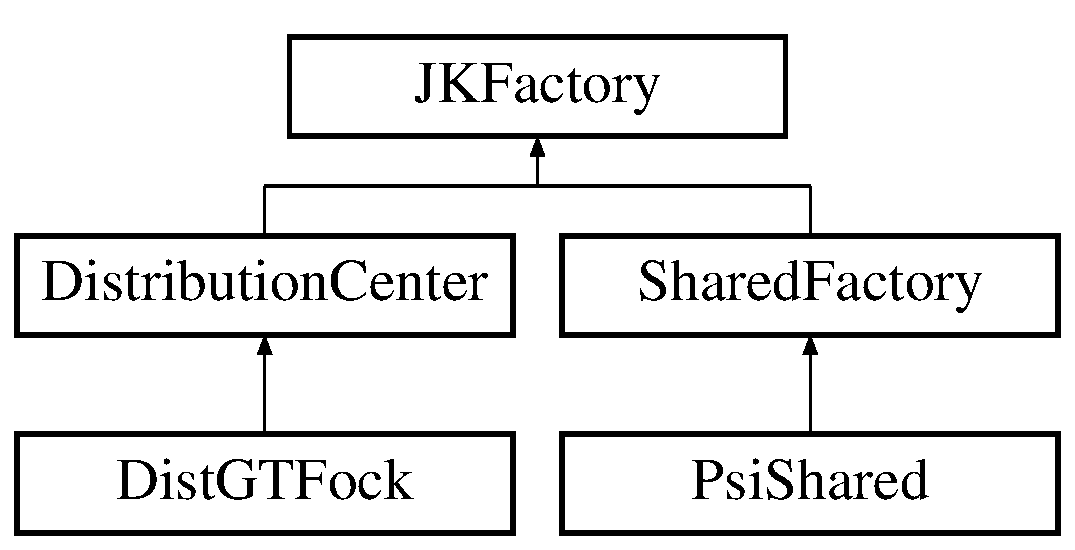
\includegraphics[height=3cm]{classJKBuilder_1_1JKFactory}
\end{center}
\end{figure}
\subsection*{Public Member Functions}
\begin{DoxyCompactItemize}
\item 
virtual void \hyperlink{classJKBuilder_1_1JKFactory_ae253b309dafe3ce003fdabfd315318b8}{BuildJK} (const double $\ast$DensityMatrix, \hyperlink{namespaceJKBuilder_aef21bc37b7cf7bc5ebb5a48628db8d0f}{SharedSymJKMatrix} \&J\_\-Matrix, \hyperlink{namespaceJKBuilder_aef21bc37b7cf7bc5ebb5a48628db8d0f}{SharedSymJKMatrix} \&K\_\-Matrix)=0
\begin{DoxyCompactList}\small\item\em The function actually in charge of building the J and K matrices. \item\end{DoxyCompactList}\item 
\hyperlink{classJKBuilder_1_1JKFactory_a05f3bfba8a8e2c8182393027e6cbbd5c}{JKFactory} ()
\begin{DoxyCompactList}\small\item\em No set up for this class. \item\end{DoxyCompactList}\item 
virtual \hyperlink{classJKBuilder_1_1JKFactory_a9350f429f8b82b14409553f0a2245a7b}{$\sim$JKFactory} ()
\begin{DoxyCompactList}\small\item\em Nothing to destroy for this class. \item\end{DoxyCompactList}\end{DoxyCompactItemize}


\subsection{Detailed Description}
The \hyperlink{classJKBuilder_1_1JKFactory}{JKFactory} class is an abstract base class that is responsible for building the J and K matrices. 

\subsection{Constructor \& Destructor Documentation}
\hypertarget{classJKBuilder_1_1JKFactory_a05f3bfba8a8e2c8182393027e6cbbd5c}{
\index{JKBuilder::JKFactory@{JKBuilder::JKFactory}!JKFactory@{JKFactory}}
\index{JKFactory@{JKFactory}!JKBuilder::JKFactory@{JKBuilder::JKFactory}}
\subsubsection[{JKFactory}]{\setlength{\rightskip}{0pt plus 5cm}{\bf JKFactory} ()}}
\label{classJKBuilder_1_1JKFactory_a05f3bfba8a8e2c8182393027e6cbbd5c}


No set up for this class. \hypertarget{classJKBuilder_1_1JKFactory_a9350f429f8b82b14409553f0a2245a7b}{
\index{JKBuilder::JKFactory@{JKBuilder::JKFactory}!$\sim$JKFactory@{$\sim$JKFactory}}
\index{$\sim$JKFactory@{$\sim$JKFactory}!JKBuilder::JKFactory@{JKBuilder::JKFactory}}
\subsubsection[{$\sim$JKFactory}]{\setlength{\rightskip}{0pt plus 5cm}$\sim${\bf JKFactory} ()\hspace{0.3cm}{\ttfamily  \mbox{[}virtual\mbox{]}}}}
\label{classJKBuilder_1_1JKFactory_a9350f429f8b82b14409553f0a2245a7b}


Nothing to destroy for this class. 

\subsection{Member Function Documentation}
\hypertarget{classJKBuilder_1_1JKFactory_ae253b309dafe3ce003fdabfd315318b8}{
\index{JKBuilder::JKFactory@{JKBuilder::JKFactory}!BuildJK@{BuildJK}}
\index{BuildJK@{BuildJK}!JKBuilder::JKFactory@{JKBuilder::JKFactory}}
\subsubsection[{BuildJK}]{\setlength{\rightskip}{0pt plus 5cm}virtual void BuildJK (const double $\ast$ {\em DensityMatrix}, \/  {\bf SharedSymJKMatrix} \& {\em J\_\-Matrix}, \/  {\bf SharedSymJKMatrix} \& {\em K\_\-Matrix})\hspace{0.3cm}{\ttfamily  \mbox{[}pure virtual\mbox{]}}}}
\label{classJKBuilder_1_1JKFactory_ae253b309dafe3ce003fdabfd315318b8}


The function actually in charge of building the J and K matrices. This function first updates the density \hyperlink{classJKBuilder_1_1matrix}{matrix} to be the one given to it. Next, it computes J and K and returns them as \hyperlink{classJKBuilder_1_1matrix}{matrix} objects.


\begin{DoxyParams}{Parameters}
\item[\mbox{$\leftarrow$} {\em DensityMatrix}]The density \hyperlink{classJKBuilder_1_1matrix}{matrix} \item[\mbox{$\rightarrow$} {\em J}]The Coulomb \hyperlink{classJKBuilder_1_1matrix}{matrix} corresponding to DensityMatrix \item[\mbox{$\rightarrow$} {\em K}]The Exchange \hyperlink{classJKBuilder_1_1matrix}{matrix} corresponding to DensityMatrix \end{DoxyParams}


Implemented in \hyperlink{classGTFock_1_1DistGTFock_aea85d0b3d84e8e52819e8a15201e078a}{DistGTFock}, and \hyperlink{classJKBuilder_1_1PsiShared_aa5f73a8109ec88464262262164feda1e}{PsiShared}.

The documentation for this class was generated from the following files:\begin{DoxyCompactItemize}
\item 
src/\hyperlink{JKFactory_8h}{JKFactory.h}\item 
src/\hyperlink{JKFactory_8cpp}{JKFactory.cpp}\end{DoxyCompactItemize}

\hypertarget{classJKBuilder_1_1Mathmatician}{
\section{Mathmatician Class Reference}
\label{classJKBuilder_1_1Mathmatician}\index{JKBuilder::Mathmatician@{JKBuilder::Mathmatician}}
}


Mathmatician's are responsible for doing math-\/y things (basically class is the interface to the math library).  


{\ttfamily \#include $<$Mathmatician.h$>$}\subsection*{Public Member Functions}
\begin{DoxyCompactItemize}
\item 
void \hyperlink{classJKBuilder_1_1Mathmatician_a2fdf5c8c21c798896b5b9d22008340f1}{scale} (\hyperlink{classJKBuilder_1_1matrix}{matrix} $\ast$matrix2scale, const double alpha)
\item 
void \hyperlink{classJKBuilder_1_1Mathmatician_a0fa0e1a12b380900f029c0007ac3d218}{copy} (\hyperlink{classJKBuilder_1_1tensor}{tensor} $\ast$To, const \hyperlink{classJKBuilder_1_1tensor}{tensor} $\ast$From)
\end{DoxyCompactItemize}


\subsection{Detailed Description}
Mathmatician's are responsible for doing math-\/y things (basically class is the interface to the math library). 

\subsection{Member Function Documentation}
\hypertarget{classJKBuilder_1_1Mathmatician_a2fdf5c8c21c798896b5b9d22008340f1}{
\index{JKBuilder::Mathmatician@{JKBuilder::Mathmatician}!scale@{scale}}
\index{scale@{scale}!JKBuilder::Mathmatician@{JKBuilder::Mathmatician}}
\subsubsection[{scale}]{\setlength{\rightskip}{0pt plus 5cm}void scale ({\bf matrix} $\ast$ {\em matrix2scale}, \/  const double {\em alpha})}}
\label{classJKBuilder_1_1Mathmatician_a2fdf5c8c21c798896b5b9d22008340f1}
\hypertarget{classJKBuilder_1_1Mathmatician_a0fa0e1a12b380900f029c0007ac3d218}{
\index{JKBuilder::Mathmatician@{JKBuilder::Mathmatician}!copy@{copy}}
\index{copy@{copy}!JKBuilder::Mathmatician@{JKBuilder::Mathmatician}}
\subsubsection[{copy}]{\setlength{\rightskip}{0pt plus 5cm}void copy ({\bf tensor} $\ast$ {\em To}, \/  const {\bf tensor} $\ast$ {\em From})}}
\label{classJKBuilder_1_1Mathmatician_a0fa0e1a12b380900f029c0007ac3d218}


The documentation for this class was generated from the following files:\begin{DoxyCompactItemize}
\item 
src/\hyperlink{Mathmatician_8h}{Mathmatician.h}\item 
src/\hyperlink{Mathmatician_8cpp}{Mathmatician.cpp}\end{DoxyCompactItemize}

\hypertarget{classJKBuilder_1_1matrix}{
\section{matrix Class Reference}
\label{classJKBuilder_1_1matrix}\index{JKBuilder::matrix@{JKBuilder::matrix}}
}


{\ttfamily \#include $<$matrix.h$>$}Inheritance diagram for matrix::\begin{figure}[H]
\begin{center}
\leavevmode
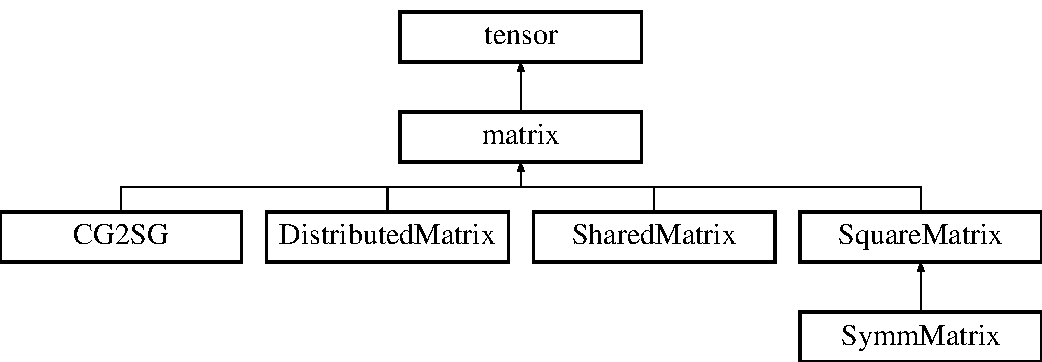
\includegraphics[height=4cm]{classJKBuilder_1_1matrix}
\end{center}
\end{figure}
\subsection*{Public Member Functions}
\begin{DoxyCompactItemize}
\item 
\hyperlink{classJKBuilder_1_1matrix_a7af07ab4ff5c2add0ae9bbf90c06c5d7}{matrix} (const int i, const int j, const bool Init=false)
\begin{DoxyCompactList}\small\item\em Makes an i by j \hyperlink{classJKBuilder_1_1matrix}{matrix} initialized to 0 if Init is set to true (defaults to false). \item\end{DoxyCompactList}\item 
\hyperlink{classJKBuilder_1_1matrix_a89f63b8297dc93a94fb0d221521fce0e}{matrix} (const double $\ast$DaMatrix, const int n, const int m)
\begin{DoxyCompactList}\small\item\em Makes an n by m \hyperlink{classJKBuilder_1_1matrix}{matrix} by copying DaMatrix. \item\end{DoxyCompactList}\item 
\hyperlink{classJKBuilder_1_1matrix_a752ebd9a51439abd10e09ff48df7e180}{matrix} (double $\ast$DaMatrix, const int n, const int m)
\begin{DoxyCompactList}\small\item\em Sets this \hyperlink{classJKBuilder_1_1matrix}{matrix} equal to the n by m \hyperlink{classJKBuilder_1_1matrix}{matrix} DaMatrix. \item\end{DoxyCompactList}\item 
\hyperlink{classJKBuilder_1_1matrix_aff55091606b5db4c54b83a04033182d7}{matrix} (const \hyperlink{classJKBuilder_1_1matrix}{matrix} \&other)
\begin{DoxyCompactList}\small\item\em Makes this \hyperlink{classJKBuilder_1_1matrix}{matrix} a copy of other. \item\end{DoxyCompactList}\item 
void \hyperlink{classJKBuilder_1_1matrix_af2563817f6505e9f8a6ee5c5c209a115}{T} ()
\begin{DoxyCompactList}\small\item\em Transposes a \hyperlink{classJKBuilder_1_1matrix}{matrix} by flipping the flag (don't forget to un-\/transpose it). \item\end{DoxyCompactList}\item 
const double \& \hyperlink{classJKBuilder_1_1matrix_a9ccbac42f4eefb704f04886001f4fb3e}{operator()} (const int i, const int j) const 
\begin{DoxyCompactList}\small\item\em Returns a non-\/editable element (i,j). \item\end{DoxyCompactList}\item 
double \& \hyperlink{classJKBuilder_1_1matrix_a3d7fca183ff1c9f4c160218746f2ef31}{operator()} (const int i, const int j)
\begin{DoxyCompactList}\small\item\em Returns an editable element (i,j). \item\end{DoxyCompactList}\item 
\hyperlink{classJKBuilder_1_1matrix}{matrix} \& \hyperlink{classJKBuilder_1_1matrix_a11df53cc3fc568369a9f612cfb556680}{operator=} (const \hyperlink{classJKBuilder_1_1matrix}{matrix} \&other)
\begin{DoxyCompactList}\small\item\em Makes this \hyperlink{classJKBuilder_1_1tensor}{tensor} a copy of other. \item\end{DoxyCompactList}\item 
\hyperlink{classJKBuilder_1_1matrix}{matrix} \& \hyperlink{classJKBuilder_1_1matrix_ad4799cbe4a5d07c77f41857a3ce914a2}{operator$\ast$} (const double alpha)
\begin{DoxyCompactList}\small\item\em Scales a \hyperlink{classJKBuilder_1_1matrix}{matrix} by alpha. \item\end{DoxyCompactList}\item 
void \hyperlink{classJKBuilder_1_1tensor_a0ca5cbe96d2a61f06ae4b543ef84f166}{Alloc} ()
\item 
bool \hyperlink{classJKBuilder_1_1tensor_a79c9a36acc5dbeab94033ca97971dc09}{IsSet} () const 
\begin{DoxyCompactList}\small\item\em Returns true if this \hyperlink{classJKBuilder_1_1tensor}{tensor} is allocated and DimsGood==true (roughly the equiv to asking if this is NULL). \item\end{DoxyCompactList}\item 
virtual void \hyperlink{classJKBuilder_1_1tensor_a98b1050f09da390896f964fb7a892391}{Initialize} ()
\begin{DoxyCompactList}\small\item\em Sets all elements to zero in the \hyperlink{classJKBuilder_1_1tensor}{tensor}, which obviously overwrites the contents. \item\end{DoxyCompactList}\item 
virtual void \hyperlink{classJKBuilder_1_1tensor_a10ffea2bf428adfa3e8319646c44a3c6}{Update} (const double $\ast$Tensor)
\begin{DoxyCompactList}\small\item\em Updates DaTensor so that it is the same as Tensor. \item\end{DoxyCompactList}\item 
int \hyperlink{classJKBuilder_1_1tensor_a537b2f14296e2f0e62f00e1703c5fa08}{TotalElements} ()
\item 
int \hyperlink{classJKBuilder_1_1tensor_a6bdcfca6493bc217b607317dbceb28b2}{DimI} (const int i) const 
\begin{DoxyCompactList}\small\item\em Returns dimension i (counting from 0). \item\end{DoxyCompactList}\item 
void \hyperlink{classJKBuilder_1_1tensor_ace6bcf62c74395ab9e37abc4935f66e0}{SetDimensions} (const int $\ast$DesiredDimensions)
\begin{DoxyCompactList}\small\item\em Copies the dimensions you want (DesiredDimensions), into the \hyperlink{classJKBuilder_1_1tensor_a2ce1e6e0782ddee097f2c4aa2663d3e9}{tensor::dimensions}. Overwrites the contents. \item\end{DoxyCompactList}\item 
virtual void \hyperlink{classJKBuilder_1_1tensor_a388f572c62279f839ee138a9afbdeeb5}{print} ()
\begin{DoxyCompactList}\small\item\em Debugging function that prints the \hyperlink{classJKBuilder_1_1tensor}{tensor} (current model not appropriate for a distributed \hyperlink{classJKBuilder_1_1tensor}{tensor}) to the \hyperlink{classJKBuilder_1_1printer}{printer}. \item\end{DoxyCompactList}\item 
virtual void \hyperlink{classJKBuilder_1_1tensor_a74b2fe351a5444c1325870dc6162f451}{print} (\hyperlink{classJKBuilder_1_1IOManager}{IOManager} \&output)
\begin{DoxyCompactList}\small\item\em Allows the user to select the destination of the printed \hyperlink{classJKBuilder_1_1tensor}{tensor}. \item\end{DoxyCompactList}\item 
const double \& \hyperlink{classJKBuilder_1_1tensor_a4f0dc1b84b580cec49500c70f87e084a}{operator\mbox{[}$\,$\mbox{]}} (const int i) const 
\begin{DoxyCompactList}\small\item\em Returns a non-\/modifiable element i of the \hyperlink{classJKBuilder_1_1tensor}{tensor}. \item\end{DoxyCompactList}\item 
double \& \hyperlink{classJKBuilder_1_1tensor_a38c9fed6b117f7cf8b76785648d76b62}{operator\mbox{[}$\,$\mbox{]}} (const int i)
\begin{DoxyCompactList}\small\item\em Returns a modifiable element i of the \hyperlink{classJKBuilder_1_1tensor}{tensor}. \item\end{DoxyCompactList}\item 
bool \hyperlink{classJKBuilder_1_1tensor_a10ae0b61e655854d12c6465d2b9e3506}{operator==} (const \hyperlink{classJKBuilder_1_1tensor}{tensor} \&other)
\begin{DoxyCompactList}\small\item\em Returns true iff this \hyperlink{classJKBuilder_1_1tensor}{tensor} is equal to the other one. \item\end{DoxyCompactList}\item 
bool \hyperlink{classJKBuilder_1_1tensor_a9b42dd835ddf2eb1a26b5d525b59b2b8}{operator!=} (const \hyperlink{classJKBuilder_1_1tensor}{tensor} \&other)
\begin{DoxyCompactList}\small\item\em Returns the opposite of operator==. \item\end{DoxyCompactList}\item 
const double $\ast$ \hyperlink{classJKBuilder_1_1tensor_a6a4e024f566d3bf9ba32a349afc5bbcf}{Address} () const 
\begin{DoxyCompactList}\small\item\em Returns the starting address of the actual data so that pointers can just be passed. \item\end{DoxyCompactList}\item 
double $\ast$ \hyperlink{classJKBuilder_1_1tensor_ac982d9eb84092bfc13694448dd824cbc}{Address} ()
\end{DoxyCompactItemize}
\subsection*{Protected Member Functions}
\begin{DoxyCompactItemize}
\item 
bool \hyperlink{classJKBuilder_1_1tensor_a6e72344440b411f433eb50171648c2d0}{DimsGood} () const 
\begin{DoxyCompactList}\small\item\em Returns true if the dimensions appear set (dimensions!=NULL \&\& dimensions\mbox{[}i\mbox{]}$>$0 for all i). \item\end{DoxyCompactList}\end{DoxyCompactItemize}
\subsection*{Protected Attributes}
\begin{DoxyCompactItemize}
\item 
bool \hyperlink{classJKBuilder_1_1matrix_a77fa48e57c519482de2ec7ec182b16ef}{IsTransposed}
\begin{DoxyCompactList}\small\item\em A flag that tells us if our \hyperlink{classJKBuilder_1_1matrix}{matrix} is transposed. \item\end{DoxyCompactList}\item 
int \hyperlink{classJKBuilder_1_1tensor_a6cfd95afd0afebd625b889fb6e58371c}{rank}
\begin{DoxyCompactList}\small\item\em This is the rank of the \hyperlink{classJKBuilder_1_1tensor}{tensor}. \item\end{DoxyCompactList}\item 
double $\ast$ \hyperlink{classJKBuilder_1_1tensor_a91f7b1e58c0e5d1a49ddb8b80ab7790e}{DaTensor}
\begin{DoxyCompactList}\small\item\em Realistically we are going to want to use this for doubles, so I am not declaring this a template. \item\end{DoxyCompactList}\item 
int \hyperlink{classJKBuilder_1_1tensor_a23ae6a00bed19d2ad34d439636e797da}{nelements}
\begin{DoxyCompactList}\small\item\em This is the total number of elements in the \hyperlink{classJKBuilder_1_1tensor}{tensor}. \item\end{DoxyCompactList}\item 
int $\ast$ \hyperlink{classJKBuilder_1_1tensor_a2ce1e6e0782ddee097f2c4aa2663d3e9}{dimensions}
\begin{DoxyCompactList}\small\item\em This is the array of \hyperlink{classJKBuilder_1_1tensor}{tensor} dimensions (row,column). \item\end{DoxyCompactList}\end{DoxyCompactItemize}
\subsection*{Private Member Functions}
\begin{DoxyCompactItemize}
\item 
void \hyperlink{classJKBuilder_1_1matrix_a065caae828723eb0040120cb077780c5}{SetUp} (const int n, const int m)
\item 
void \hyperlink{classJKBuilder_1_1matrix_a75177328107f96ec679d43fce0a9e866}{Copy} (const \hyperlink{classJKBuilder_1_1matrix}{matrix} \&other)
\begin{DoxyCompactList}\small\item\em The function that actually copies the \hyperlink{classJKBuilder_1_1tensor}{tensor}. Do not use if you just want to pass pointers around, cause it copies (duh...). \item\end{DoxyCompactList}\end{DoxyCompactItemize}


\subsection{Constructor \& Destructor Documentation}
\hypertarget{classJKBuilder_1_1matrix_a7af07ab4ff5c2add0ae9bbf90c06c5d7}{
\index{JKBuilder::matrix@{JKBuilder::matrix}!matrix@{matrix}}
\index{matrix@{matrix}!JKBuilder::matrix@{JKBuilder::matrix}}
\subsubsection[{matrix}]{\setlength{\rightskip}{0pt plus 5cm}{\bf matrix} (const int {\em i}, \/  const int {\em j}, \/  const bool {\em Init} = {\ttfamily false})}}
\label{classJKBuilder_1_1matrix_a7af07ab4ff5c2add0ae9bbf90c06c5d7}


Makes an i by j \hyperlink{classJKBuilder_1_1matrix}{matrix} initialized to 0 if Init is set to true (defaults to false). \hypertarget{classJKBuilder_1_1matrix_a89f63b8297dc93a94fb0d221521fce0e}{
\index{JKBuilder::matrix@{JKBuilder::matrix}!matrix@{matrix}}
\index{matrix@{matrix}!JKBuilder::matrix@{JKBuilder::matrix}}
\subsubsection[{matrix}]{\setlength{\rightskip}{0pt plus 5cm}{\bf matrix} (const double $\ast$ {\em DaMatrix}, \/  const int {\em n}, \/  const int {\em m})}}
\label{classJKBuilder_1_1matrix_a89f63b8297dc93a94fb0d221521fce0e}


Makes an n by m \hyperlink{classJKBuilder_1_1matrix}{matrix} by copying DaMatrix. \hypertarget{classJKBuilder_1_1matrix_a752ebd9a51439abd10e09ff48df7e180}{
\index{JKBuilder::matrix@{JKBuilder::matrix}!matrix@{matrix}}
\index{matrix@{matrix}!JKBuilder::matrix@{JKBuilder::matrix}}
\subsubsection[{matrix}]{\setlength{\rightskip}{0pt plus 5cm}{\bf matrix} (double $\ast$ {\em DaMatrix}, \/  const int {\em n}, \/  const int {\em m})}}
\label{classJKBuilder_1_1matrix_a752ebd9a51439abd10e09ff48df7e180}


Sets this \hyperlink{classJKBuilder_1_1matrix}{matrix} equal to the n by m \hyperlink{classJKBuilder_1_1matrix}{matrix} DaMatrix. 

Just take the pointer \hypertarget{classJKBuilder_1_1matrix_aff55091606b5db4c54b83a04033182d7}{
\index{JKBuilder::matrix@{JKBuilder::matrix}!matrix@{matrix}}
\index{matrix@{matrix}!JKBuilder::matrix@{JKBuilder::matrix}}
\subsubsection[{matrix}]{\setlength{\rightskip}{0pt plus 5cm}{\bf matrix} (const {\bf matrix} \& {\em other})}}
\label{classJKBuilder_1_1matrix_aff55091606b5db4c54b83a04033182d7}


Makes this \hyperlink{classJKBuilder_1_1matrix}{matrix} a copy of other. 

\subsection{Member Function Documentation}
\hypertarget{classJKBuilder_1_1matrix_a065caae828723eb0040120cb077780c5}{
\index{JKBuilder::matrix@{JKBuilder::matrix}!SetUp@{SetUp}}
\index{SetUp@{SetUp}!JKBuilder::matrix@{JKBuilder::matrix}}
\subsubsection[{SetUp}]{\setlength{\rightskip}{0pt plus 5cm}void SetUp (const int {\em n}, \/  const int {\em m})\hspace{0.3cm}{\ttfamily  \mbox{[}private\mbox{]}}}}
\label{classJKBuilder_1_1matrix_a065caae828723eb0040120cb077780c5}
\hypertarget{classJKBuilder_1_1matrix_a75177328107f96ec679d43fce0a9e866}{
\index{JKBuilder::matrix@{JKBuilder::matrix}!Copy@{Copy}}
\index{Copy@{Copy}!JKBuilder::matrix@{JKBuilder::matrix}}
\subsubsection[{Copy}]{\setlength{\rightskip}{0pt plus 5cm}void Copy (const {\bf matrix} \& {\em other})\hspace{0.3cm}{\ttfamily  \mbox{[}private\mbox{]}}}}
\label{classJKBuilder_1_1matrix_a75177328107f96ec679d43fce0a9e866}


The function that actually copies the \hyperlink{classJKBuilder_1_1tensor}{tensor}. Do not use if you just want to pass pointers around, cause it copies (duh...). 

Reimplemented from \hyperlink{classJKBuilder_1_1tensor_a60e1f7417550ba45971b688cc168d34f}{tensor}.

Reimplemented in \hyperlink{classJKBuilder_1_1SymmMatrix_a7be0365900350f51e54969bb1961af8f}{SymmMatrix}.\hypertarget{classJKBuilder_1_1matrix_af2563817f6505e9f8a6ee5c5c209a115}{
\index{JKBuilder::matrix@{JKBuilder::matrix}!T@{T}}
\index{T@{T}!JKBuilder::matrix@{JKBuilder::matrix}}
\subsubsection[{T}]{\setlength{\rightskip}{0pt plus 5cm}void T ()}}
\label{classJKBuilder_1_1matrix_af2563817f6505e9f8a6ee5c5c209a115}


Transposes a \hyperlink{classJKBuilder_1_1matrix}{matrix} by flipping the flag (don't forget to un-\/transpose it). \hypertarget{classJKBuilder_1_1matrix_a9ccbac42f4eefb704f04886001f4fb3e}{
\index{JKBuilder::matrix@{JKBuilder::matrix}!operator()@{operator()}}
\index{operator()@{operator()}!JKBuilder::matrix@{JKBuilder::matrix}}
\subsubsection[{operator()}]{\setlength{\rightskip}{0pt plus 5cm}const double \& operator() (const int {\em i}, \/  const int {\em j}) const}}
\label{classJKBuilder_1_1matrix_a9ccbac42f4eefb704f04886001f4fb3e}


Returns a non-\/editable element (i,j). 

Reimplemented in \hyperlink{classJKBuilder_1_1SymmMatrix_a9ccbac42f4eefb704f04886001f4fb3e}{SymmMatrix}.\hypertarget{classJKBuilder_1_1matrix_a3d7fca183ff1c9f4c160218746f2ef31}{
\index{JKBuilder::matrix@{JKBuilder::matrix}!operator()@{operator()}}
\index{operator()@{operator()}!JKBuilder::matrix@{JKBuilder::matrix}}
\subsubsection[{operator()}]{\setlength{\rightskip}{0pt plus 5cm}double \& operator() (const int {\em i}, \/  const int {\em j})}}
\label{classJKBuilder_1_1matrix_a3d7fca183ff1c9f4c160218746f2ef31}


Returns an editable element (i,j). 

Reimplemented in \hyperlink{classJKBuilder_1_1SymmMatrix_a3d7fca183ff1c9f4c160218746f2ef31}{SymmMatrix}.\hypertarget{classJKBuilder_1_1matrix_a11df53cc3fc568369a9f612cfb556680}{
\index{JKBuilder::matrix@{JKBuilder::matrix}!operator=@{operator=}}
\index{operator=@{operator=}!JKBuilder::matrix@{JKBuilder::matrix}}
\subsubsection[{operator=}]{\setlength{\rightskip}{0pt plus 5cm}{\bf matrix} \& operator= (const {\bf matrix} \& {\em other})}}
\label{classJKBuilder_1_1matrix_a11df53cc3fc568369a9f612cfb556680}


Makes this \hyperlink{classJKBuilder_1_1tensor}{tensor} a copy of other. 

Reimplemented from \hyperlink{classJKBuilder_1_1tensor_a29113cbfe726b02b94576f631c983386}{tensor}.

Reimplemented in \hyperlink{classJKBuilder_1_1SquareMatrix_ad78e5a12d26f1984d77a57095bc4d181}{SquareMatrix}, and \hyperlink{classJKBuilder_1_1SymmMatrix_aca4a8297278ff39c5422febf1dcbc5ac}{SymmMatrix}.\hypertarget{classJKBuilder_1_1matrix_ad4799cbe4a5d07c77f41857a3ce914a2}{
\index{JKBuilder::matrix@{JKBuilder::matrix}!operator$\ast$@{operator$\ast$}}
\index{operator$\ast$@{operator$\ast$}!JKBuilder::matrix@{JKBuilder::matrix}}
\subsubsection[{operator$\ast$}]{\setlength{\rightskip}{0pt plus 5cm}{\bf matrix} \& operator$\ast$ (const double {\em alpha})}}
\label{classJKBuilder_1_1matrix_ad4799cbe4a5d07c77f41857a3ce914a2}


Scales a \hyperlink{classJKBuilder_1_1matrix}{matrix} by alpha. \hypertarget{classJKBuilder_1_1tensor_a6e72344440b411f433eb50171648c2d0}{
\index{JKBuilder::matrix@{JKBuilder::matrix}!DimsGood@{DimsGood}}
\index{DimsGood@{DimsGood}!JKBuilder::matrix@{JKBuilder::matrix}}
\subsubsection[{DimsGood}]{\setlength{\rightskip}{0pt plus 5cm}bool DimsGood () const\hspace{0.3cm}{\ttfamily  \mbox{[}protected, inherited\mbox{]}}}}
\label{classJKBuilder_1_1tensor_a6e72344440b411f433eb50171648c2d0}


Returns true if the dimensions appear set (dimensions!=NULL \&\& dimensions\mbox{[}i\mbox{]}$>$0 for all i). \hypertarget{classJKBuilder_1_1tensor_a0ca5cbe96d2a61f06ae4b543ef84f166}{
\index{JKBuilder::matrix@{JKBuilder::matrix}!Alloc@{Alloc}}
\index{Alloc@{Alloc}!JKBuilder::matrix@{JKBuilder::matrix}}
\subsubsection[{Alloc}]{\setlength{\rightskip}{0pt plus 5cm}void Alloc ()\hspace{0.3cm}{\ttfamily  \mbox{[}inherited\mbox{]}}}}
\label{classJKBuilder_1_1tensor_a0ca5cbe96d2a61f06ae4b543ef84f166}
The following function can never be virtual because base operations of the Tensor depend on them The actual memory allocation call, if DaTensor==NULL allocates the memory \hypertarget{classJKBuilder_1_1tensor_a79c9a36acc5dbeab94033ca97971dc09}{
\index{JKBuilder::matrix@{JKBuilder::matrix}!IsSet@{IsSet}}
\index{IsSet@{IsSet}!JKBuilder::matrix@{JKBuilder::matrix}}
\subsubsection[{IsSet}]{\setlength{\rightskip}{0pt plus 5cm}bool IsSet () const\hspace{0.3cm}{\ttfamily  \mbox{[}inherited\mbox{]}}}}
\label{classJKBuilder_1_1tensor_a79c9a36acc5dbeab94033ca97971dc09}


Returns true if this \hyperlink{classJKBuilder_1_1tensor}{tensor} is allocated and DimsGood==true (roughly the equiv to asking if this is NULL). \hypertarget{classJKBuilder_1_1tensor_a98b1050f09da390896f964fb7a892391}{
\index{JKBuilder::matrix@{JKBuilder::matrix}!Initialize@{Initialize}}
\index{Initialize@{Initialize}!JKBuilder::matrix@{JKBuilder::matrix}}
\subsubsection[{Initialize}]{\setlength{\rightskip}{0pt plus 5cm}void Initialize ()\hspace{0.3cm}{\ttfamily  \mbox{[}virtual, inherited\mbox{]}}}}
\label{classJKBuilder_1_1tensor_a98b1050f09da390896f964fb7a892391}


Sets all elements to zero in the \hyperlink{classJKBuilder_1_1tensor}{tensor}, which obviously overwrites the contents. 

Reimplemented in \hyperlink{classJKBuilder_1_1DistributedMatrix_a98b1050f09da390896f964fb7a892391}{DistributedMatrix}.\hypertarget{classJKBuilder_1_1tensor_a10ffea2bf428adfa3e8319646c44a3c6}{
\index{JKBuilder::matrix@{JKBuilder::matrix}!Update@{Update}}
\index{Update@{Update}!JKBuilder::matrix@{JKBuilder::matrix}}
\subsubsection[{Update}]{\setlength{\rightskip}{0pt plus 5cm}void Update (const double $\ast$ {\em Tensor})\hspace{0.3cm}{\ttfamily  \mbox{[}virtual, inherited\mbox{]}}}}
\label{classJKBuilder_1_1tensor_a10ffea2bf428adfa3e8319646c44a3c6}


Updates DaTensor so that it is the same as Tensor. Update always takes the full Tensor, not a block of it. It is child class's jobs to scatter the data if need be. 

Reimplemented in \hyperlink{classJKBuilder_1_1DistributedMatrix_a6a378face23ba83b2431cb08e8519066}{DistributedMatrix}.\hypertarget{classJKBuilder_1_1tensor_a537b2f14296e2f0e62f00e1703c5fa08}{
\index{JKBuilder::matrix@{JKBuilder::matrix}!TotalElements@{TotalElements}}
\index{TotalElements@{TotalElements}!JKBuilder::matrix@{JKBuilder::matrix}}
\subsubsection[{TotalElements}]{\setlength{\rightskip}{0pt plus 5cm}int TotalElements ()\hspace{0.3cm}{\ttfamily  \mbox{[}inherited\mbox{]}}}}
\label{classJKBuilder_1_1tensor_a537b2f14296e2f0e62f00e1703c5fa08}
\hypertarget{classJKBuilder_1_1tensor_a6bdcfca6493bc217b607317dbceb28b2}{
\index{JKBuilder::matrix@{JKBuilder::matrix}!DimI@{DimI}}
\index{DimI@{DimI}!JKBuilder::matrix@{JKBuilder::matrix}}
\subsubsection[{DimI}]{\setlength{\rightskip}{0pt plus 5cm}int DimI (const int {\em i}) const\hspace{0.3cm}{\ttfamily  \mbox{[}inherited\mbox{]}}}}
\label{classJKBuilder_1_1tensor_a6bdcfca6493bc217b607317dbceb28b2}


Returns dimension i (counting from 0). \hypertarget{classJKBuilder_1_1tensor_ace6bcf62c74395ab9e37abc4935f66e0}{
\index{JKBuilder::matrix@{JKBuilder::matrix}!SetDimensions@{SetDimensions}}
\index{SetDimensions@{SetDimensions}!JKBuilder::matrix@{JKBuilder::matrix}}
\subsubsection[{SetDimensions}]{\setlength{\rightskip}{0pt plus 5cm}void SetDimensions (const int $\ast$ {\em DesiredDimensions})\hspace{0.3cm}{\ttfamily  \mbox{[}inherited\mbox{]}}}}
\label{classJKBuilder_1_1tensor_ace6bcf62c74395ab9e37abc4935f66e0}


Copies the dimensions you want (DesiredDimensions), into the \hyperlink{classJKBuilder_1_1tensor_a2ce1e6e0782ddee097f2c4aa2663d3e9}{tensor::dimensions}. Overwrites the contents. \hypertarget{classJKBuilder_1_1tensor_a388f572c62279f839ee138a9afbdeeb5}{
\index{JKBuilder::matrix@{JKBuilder::matrix}!print@{print}}
\index{print@{print}!JKBuilder::matrix@{JKBuilder::matrix}}
\subsubsection[{print}]{\setlength{\rightskip}{0pt plus 5cm}void print ()\hspace{0.3cm}{\ttfamily  \mbox{[}virtual, inherited\mbox{]}}}}
\label{classJKBuilder_1_1tensor_a388f572c62279f839ee138a9afbdeeb5}


Debugging function that prints the \hyperlink{classJKBuilder_1_1tensor}{tensor} (current model not appropriate for a distributed \hyperlink{classJKBuilder_1_1tensor}{tensor}) to the \hyperlink{classJKBuilder_1_1printer}{printer}. 

Reimplemented in \hyperlink{classJKBuilder_1_1DistributedMatrix_a388f572c62279f839ee138a9afbdeeb5}{DistributedMatrix}.\hypertarget{classJKBuilder_1_1tensor_a74b2fe351a5444c1325870dc6162f451}{
\index{JKBuilder::matrix@{JKBuilder::matrix}!print@{print}}
\index{print@{print}!JKBuilder::matrix@{JKBuilder::matrix}}
\subsubsection[{print}]{\setlength{\rightskip}{0pt plus 5cm}void print ({\bf IOManager} \& {\em output})\hspace{0.3cm}{\ttfamily  \mbox{[}virtual, inherited\mbox{]}}}}
\label{classJKBuilder_1_1tensor_a74b2fe351a5444c1325870dc6162f451}


Allows the user to select the destination of the printed \hyperlink{classJKBuilder_1_1tensor}{tensor}. 

Reimplemented in \hyperlink{classJKBuilder_1_1DistributedMatrix_a74b2fe351a5444c1325870dc6162f451}{DistributedMatrix}.\hypertarget{classJKBuilder_1_1tensor_a4f0dc1b84b580cec49500c70f87e084a}{
\index{JKBuilder::matrix@{JKBuilder::matrix}!operator\mbox{[}\mbox{]}@{operator[]}}
\index{operator\mbox{[}\mbox{]}@{operator[]}!JKBuilder::matrix@{JKBuilder::matrix}}
\subsubsection[{operator[]}]{\setlength{\rightskip}{0pt plus 5cm}const double \& operator\mbox{[}$\,$\mbox{]} (const int {\em i}) const\hspace{0.3cm}{\ttfamily  \mbox{[}inherited\mbox{]}}}}
\label{classJKBuilder_1_1tensor_a4f0dc1b84b580cec49500c70f87e084a}


Returns a non-\/modifiable element i of the \hyperlink{classJKBuilder_1_1tensor}{tensor}. \hypertarget{classJKBuilder_1_1tensor_a38c9fed6b117f7cf8b76785648d76b62}{
\index{JKBuilder::matrix@{JKBuilder::matrix}!operator\mbox{[}\mbox{]}@{operator[]}}
\index{operator\mbox{[}\mbox{]}@{operator[]}!JKBuilder::matrix@{JKBuilder::matrix}}
\subsubsection[{operator[]}]{\setlength{\rightskip}{0pt plus 5cm}double \& operator\mbox{[}$\,$\mbox{]} (const int {\em i})\hspace{0.3cm}{\ttfamily  \mbox{[}inherited\mbox{]}}}}
\label{classJKBuilder_1_1tensor_a38c9fed6b117f7cf8b76785648d76b62}


Returns a modifiable element i of the \hyperlink{classJKBuilder_1_1tensor}{tensor}. \hypertarget{classJKBuilder_1_1tensor_a10ae0b61e655854d12c6465d2b9e3506}{
\index{JKBuilder::matrix@{JKBuilder::matrix}!operator==@{operator==}}
\index{operator==@{operator==}!JKBuilder::matrix@{JKBuilder::matrix}}
\subsubsection[{operator==}]{\setlength{\rightskip}{0pt plus 5cm}bool operator== (const {\bf tensor} \& {\em other})\hspace{0.3cm}{\ttfamily  \mbox{[}inherited\mbox{]}}}}
\label{classJKBuilder_1_1tensor_a10ae0b61e655854d12c6465d2b9e3506}


Returns true iff this \hyperlink{classJKBuilder_1_1tensor}{tensor} is equal to the other one. \hypertarget{classJKBuilder_1_1tensor_a9b42dd835ddf2eb1a26b5d525b59b2b8}{
\index{JKBuilder::matrix@{JKBuilder::matrix}!operator!=@{operator!=}}
\index{operator!=@{operator!=}!JKBuilder::matrix@{JKBuilder::matrix}}
\subsubsection[{operator!=}]{\setlength{\rightskip}{0pt plus 5cm}bool operator!= (const {\bf tensor} \& {\em other})\hspace{0.3cm}{\ttfamily  \mbox{[}inherited\mbox{]}}}}
\label{classJKBuilder_1_1tensor_a9b42dd835ddf2eb1a26b5d525b59b2b8}


Returns the opposite of operator==. \hypertarget{classJKBuilder_1_1tensor_a6a4e024f566d3bf9ba32a349afc5bbcf}{
\index{JKBuilder::matrix@{JKBuilder::matrix}!Address@{Address}}
\index{Address@{Address}!JKBuilder::matrix@{JKBuilder::matrix}}
\subsubsection[{Address}]{\setlength{\rightskip}{0pt plus 5cm}const double $\ast$ Address () const\hspace{0.3cm}{\ttfamily  \mbox{[}inherited\mbox{]}}}}
\label{classJKBuilder_1_1tensor_a6a4e024f566d3bf9ba32a349afc5bbcf}


Returns the starting address of the actual data so that pointers can just be passed. \hypertarget{classJKBuilder_1_1tensor_ac982d9eb84092bfc13694448dd824cbc}{
\index{JKBuilder::matrix@{JKBuilder::matrix}!Address@{Address}}
\index{Address@{Address}!JKBuilder::matrix@{JKBuilder::matrix}}
\subsubsection[{Address}]{\setlength{\rightskip}{0pt plus 5cm}double $\ast$ Address ()\hspace{0.3cm}{\ttfamily  \mbox{[}inherited\mbox{]}}}}
\label{classJKBuilder_1_1tensor_ac982d9eb84092bfc13694448dd824cbc}


\subsection{Member Data Documentation}
\hypertarget{classJKBuilder_1_1matrix_a77fa48e57c519482de2ec7ec182b16ef}{
\index{JKBuilder::matrix@{JKBuilder::matrix}!IsTransposed@{IsTransposed}}
\index{IsTransposed@{IsTransposed}!JKBuilder::matrix@{JKBuilder::matrix}}
\subsubsection[{IsTransposed}]{\setlength{\rightskip}{0pt plus 5cm}bool {\bf IsTransposed}\hspace{0.3cm}{\ttfamily  \mbox{[}protected\mbox{]}}}}
\label{classJKBuilder_1_1matrix_a77fa48e57c519482de2ec7ec182b16ef}


A flag that tells us if our \hyperlink{classJKBuilder_1_1matrix}{matrix} is transposed. \hypertarget{classJKBuilder_1_1tensor_a6cfd95afd0afebd625b889fb6e58371c}{
\index{JKBuilder::matrix@{JKBuilder::matrix}!rank@{rank}}
\index{rank@{rank}!JKBuilder::matrix@{JKBuilder::matrix}}
\subsubsection[{rank}]{\setlength{\rightskip}{0pt plus 5cm}int {\bf rank}\hspace{0.3cm}{\ttfamily  \mbox{[}protected, inherited\mbox{]}}}}
\label{classJKBuilder_1_1tensor_a6cfd95afd0afebd625b889fb6e58371c}


This is the rank of the \hyperlink{classJKBuilder_1_1tensor}{tensor}. \hypertarget{classJKBuilder_1_1tensor_a91f7b1e58c0e5d1a49ddb8b80ab7790e}{
\index{JKBuilder::matrix@{JKBuilder::matrix}!DaTensor@{DaTensor}}
\index{DaTensor@{DaTensor}!JKBuilder::matrix@{JKBuilder::matrix}}
\subsubsection[{DaTensor}]{\setlength{\rightskip}{0pt plus 5cm}double$\ast$ {\bf DaTensor}\hspace{0.3cm}{\ttfamily  \mbox{[}protected, inherited\mbox{]}}}}
\label{classJKBuilder_1_1tensor_a91f7b1e58c0e5d1a49ddb8b80ab7790e}


Realistically we are going to want to use this for doubles, so I am not declaring this a template. \hypertarget{classJKBuilder_1_1tensor_a23ae6a00bed19d2ad34d439636e797da}{
\index{JKBuilder::matrix@{JKBuilder::matrix}!nelements@{nelements}}
\index{nelements@{nelements}!JKBuilder::matrix@{JKBuilder::matrix}}
\subsubsection[{nelements}]{\setlength{\rightskip}{0pt plus 5cm}int {\bf nelements}\hspace{0.3cm}{\ttfamily  \mbox{[}protected, inherited\mbox{]}}}}
\label{classJKBuilder_1_1tensor_a23ae6a00bed19d2ad34d439636e797da}


This is the total number of elements in the \hyperlink{classJKBuilder_1_1tensor}{tensor}. \hypertarget{classJKBuilder_1_1tensor_a2ce1e6e0782ddee097f2c4aa2663d3e9}{
\index{JKBuilder::matrix@{JKBuilder::matrix}!dimensions@{dimensions}}
\index{dimensions@{dimensions}!JKBuilder::matrix@{JKBuilder::matrix}}
\subsubsection[{dimensions}]{\setlength{\rightskip}{0pt plus 5cm}int$\ast$ {\bf dimensions}\hspace{0.3cm}{\ttfamily  \mbox{[}protected, inherited\mbox{]}}}}
\label{classJKBuilder_1_1tensor_a2ce1e6e0782ddee097f2c4aa2663d3e9}


This is the array of \hyperlink{classJKBuilder_1_1tensor}{tensor} dimensions (row,column). These dimensions are for the whole object, not blocks of it or anything else like that. What this means is that for say a 12 by 12 \hyperlink{classJKBuilder_1_1matrix}{matrix} distributed in 6 by 6 blocks these values are 12, not 6. 

The documentation for this class was generated from the following files:\begin{DoxyCompactItemize}
\item 
src/\hyperlink{matrix_8h}{matrix.h}\item 
src/\hyperlink{matrix_8cpp}{matrix.cpp}\end{DoxyCompactItemize}

\hypertarget{classJKBuilder_1_1molecule__class}{
\section{molecule\_\-class Class Reference}
\label{classJKBuilder_1_1molecule__class}\index{JKBuilder::molecule\_\-class@{JKBuilder::molecule\_\-class}}
}


The top level class in charge of holding molecular details.  


{\ttfamily \#include $<$molecule.h$>$}\subsection*{Public Member Functions}
\begin{DoxyCompactItemize}
\item 
void \hyperlink{classJKBuilder_1_1molecule__class_a16b721cec672dda3fc1a3c90e3d71120}{WriteGTFockXYZFile} () const 
\begin{DoxyCompactList}\small\item\em This function writes the molecule as an $\ast$.xyz file to the current directory. \item\end{DoxyCompactList}\item 
int \hyperlink{classJKBuilder_1_1molecule__class_abb0ac82b97b1f6476539eb2b712bbceb}{GetNatoms} () const 
\begin{DoxyCompactList}\small\item\em Returns the number of atoms. \item\end{DoxyCompactList}\item 
int \hyperlink{classJKBuilder_1_1molecule__class_aeb29d9144c99d302f7b43d5398929ea5}{GetNelec} () const 
\begin{DoxyCompactList}\small\item\em Returns the number of electrons $\sum_i Z_i-q$, where $q$ is the total system charge. \item\end{DoxyCompactList}\item 
const double \& \hyperlink{classJKBuilder_1_1molecule__class_a9ccbac42f4eefb704f04886001f4fb3e}{operator()} (const int i, const int j) const 
\begin{DoxyCompactList}\small\item\em Returns Cartesian coordinate j of \hyperlink{classJKBuilder_1_1atom}{atom} i (in bohr). \item\end{DoxyCompactList}\item 
const \hyperlink{classJKBuilder_1_1atom}{atom} $\ast$ \hyperlink{classJKBuilder_1_1molecule__class_a8a54a3b159b0eb733c877569b32f13e3}{operator\mbox{[}$\,$\mbox{]}} (const int i) const 
\begin{DoxyCompactList}\small\item\em Returns Atom i. \item\end{DoxyCompactList}\item 
\hyperlink{classJKBuilder_1_1molecule__class_a227b81bd92795b9926c71e77fa2e3d94}{molecule\_\-class} (const double $\ast$InCarts, const int NumAtoms, const int \hyperlink{classJKBuilder_1_1molecule__class_ae8b866d74c9f0b8464b1aee9788c04eb}{charge}=0, const bool bohr=false)
\begin{DoxyCompactList}\small\item\em Makes the molecule. \item\end{DoxyCompactList}\item 
\hyperlink{classJKBuilder_1_1molecule__class_a60295ae66e9fad98bd3feaa08a443d6d}{molecule\_\-class} ()
\begin{DoxyCompactList}\small\item\em Sets all pointers=NULL and NAtoms=0. \item\end{DoxyCompactList}\item 
\hyperlink{classJKBuilder_1_1molecule__class_ae8b7f222e2b1b67f0b5d078456e6b6bc}{$\sim$molecule\_\-class} ()
\begin{DoxyCompactList}\small\item\em Frees the memory. \item\end{DoxyCompactList}\end{DoxyCompactItemize}
\subsection*{Private Attributes}
\begin{DoxyCompactItemize}
\item 
std::vector$<$ \hyperlink{classJKBuilder_1_1atom}{atom} $\ast$ $>$ \hyperlink{classJKBuilder_1_1molecule__class_a88ab0e266efe1ae93e6005501b372c76}{atoms}
\begin{DoxyCompactList}\small\item\em The actual atoms. \item\end{DoxyCompactList}\item 
int \hyperlink{classJKBuilder_1_1molecule__class_a849e4a1d5fee0c024e42b658d3babd02}{Nelec}
\begin{DoxyCompactList}\small\item\em The total number of electrons. \item\end{DoxyCompactList}\item 
int \hyperlink{classJKBuilder_1_1molecule__class_ae8b866d74c9f0b8464b1aee9788c04eb}{charge}
\begin{DoxyCompactList}\small\item\em The charge of the system. \item\end{DoxyCompactList}\end{DoxyCompactItemize}


\subsection{Detailed Description}
The top level class in charge of holding molecular details. The \hyperlink{classJKBuilder_1_1molecule__class}{molecule\_\-class} object is basically a set of atoms (just like a real molecule). It knows the basic details of the molecule, but nothing too fancy. One key concept that is used to decrease the constructor argument list is the idea of \char`\"{}messy\char`\"{} coordinates. This is simply an Natoms by 4 array where element i,0 is the atomic number of \hyperlink{classJKBuilder_1_1atom}{atom} i, and i,1 to i,3 are the x,y, and z coordinates of \hyperlink{classJKBuilder_1_1atom}{atom} i, respectively. 

\subsection{Constructor \& Destructor Documentation}
\hypertarget{classJKBuilder_1_1molecule__class_a227b81bd92795b9926c71e77fa2e3d94}{
\index{JKBuilder::molecule\_\-class@{JKBuilder::molecule\_\-class}!molecule\_\-class@{molecule\_\-class}}
\index{molecule\_\-class@{molecule\_\-class}!JKBuilder::molecule_class@{JKBuilder::molecule\_\-class}}
\subsubsection[{molecule\_\-class}]{\setlength{\rightskip}{0pt plus 5cm}{\bf molecule\_\-class} (const double $\ast$ {\em InCarts}, \/  const int {\em NumAtoms}, \/  const int {\em charge} = {\ttfamily 0}, \/  const bool {\em bohr} = {\ttfamily false})}}
\label{classJKBuilder_1_1molecule__class_a227b81bd92795b9926c71e77fa2e3d94}


Makes the molecule. Really two parts to this constructor, first it creates a bunch of JKBuilder::atoms (natoms of them...). Then it Calculates the number of electrons by adding up the Z's of each \hyperlink{classJKBuilder_1_1atom}{atom} and subtracting out the charge.


\begin{DoxyParams}{Parameters}
\item[\mbox{$\leftarrow$} {\em InCarts}]The Cartesian coordinates, in messy form \item[\mbox{$\leftarrow$} {\em NumAtoms}]The number of atoms \item[\mbox{$\leftarrow$} {\em charge}]The charge of the molecule, in atomic units, (defaults to 0) \item[\mbox{$\leftarrow$} {\em bohr}]True means the coordinates in InCarts are in atomic units, (defaults to false) \end{DoxyParams}
\hypertarget{classJKBuilder_1_1molecule__class_a60295ae66e9fad98bd3feaa08a443d6d}{
\index{JKBuilder::molecule\_\-class@{JKBuilder::molecule\_\-class}!molecule\_\-class@{molecule\_\-class}}
\index{molecule\_\-class@{molecule\_\-class}!JKBuilder::molecule_class@{JKBuilder::molecule\_\-class}}
\subsubsection[{molecule\_\-class}]{\setlength{\rightskip}{0pt plus 5cm}{\bf molecule\_\-class} ()}}
\label{classJKBuilder_1_1molecule__class_a60295ae66e9fad98bd3feaa08a443d6d}


Sets all pointers=NULL and NAtoms=0. \hypertarget{classJKBuilder_1_1molecule__class_ae8b7f222e2b1b67f0b5d078456e6b6bc}{
\index{JKBuilder::molecule\_\-class@{JKBuilder::molecule\_\-class}!$\sim$molecule\_\-class@{$\sim$molecule\_\-class}}
\index{$\sim$molecule\_\-class@{$\sim$molecule\_\-class}!JKBuilder::molecule_class@{JKBuilder::molecule\_\-class}}
\subsubsection[{$\sim$molecule\_\-class}]{\setlength{\rightskip}{0pt plus 5cm}$\sim${\bf molecule\_\-class} ()}}
\label{classJKBuilder_1_1molecule__class_ae8b7f222e2b1b67f0b5d078456e6b6bc}


Frees the memory. 

\subsection{Member Function Documentation}
\hypertarget{classJKBuilder_1_1molecule__class_a16b721cec672dda3fc1a3c90e3d71120}{
\index{JKBuilder::molecule\_\-class@{JKBuilder::molecule\_\-class}!WriteGTFockXYZFile@{WriteGTFockXYZFile}}
\index{WriteGTFockXYZFile@{WriteGTFockXYZFile}!JKBuilder::molecule_class@{JKBuilder::molecule\_\-class}}
\subsubsection[{WriteGTFockXYZFile}]{\setlength{\rightskip}{0pt plus 5cm}void WriteGTFockXYZFile () const}}
\label{classJKBuilder_1_1molecule__class_a16b721cec672dda3fc1a3c90e3d71120}


This function writes the molecule as an $\ast$.xyz file to the current directory. In order to interface with the \hyperlink{namespaceGTFock}{GTFock} library we need an $\ast$.xyz file. This routine will make that file. Note that for whatever reason, the \hyperlink{namespaceGTFock}{GTFock} library does not include the standard comment line in the $\ast$.xyz file, so we also do not. \hypertarget{classJKBuilder_1_1molecule__class_abb0ac82b97b1f6476539eb2b712bbceb}{
\index{JKBuilder::molecule\_\-class@{JKBuilder::molecule\_\-class}!GetNatoms@{GetNatoms}}
\index{GetNatoms@{GetNatoms}!JKBuilder::molecule_class@{JKBuilder::molecule\_\-class}}
\subsubsection[{GetNatoms}]{\setlength{\rightskip}{0pt plus 5cm}int GetNatoms () const}}
\label{classJKBuilder_1_1molecule__class_abb0ac82b97b1f6476539eb2b712bbceb}


Returns the number of atoms. \hypertarget{classJKBuilder_1_1molecule__class_aeb29d9144c99d302f7b43d5398929ea5}{
\index{JKBuilder::molecule\_\-class@{JKBuilder::molecule\_\-class}!GetNelec@{GetNelec}}
\index{GetNelec@{GetNelec}!JKBuilder::molecule_class@{JKBuilder::molecule\_\-class}}
\subsubsection[{GetNelec}]{\setlength{\rightskip}{0pt plus 5cm}int GetNelec () const}}
\label{classJKBuilder_1_1molecule__class_aeb29d9144c99d302f7b43d5398929ea5}


Returns the number of electrons $\sum_i Z_i-q$, where $q$ is the total system charge. \hypertarget{classJKBuilder_1_1molecule__class_a9ccbac42f4eefb704f04886001f4fb3e}{
\index{JKBuilder::molecule\_\-class@{JKBuilder::molecule\_\-class}!operator()@{operator()}}
\index{operator()@{operator()}!JKBuilder::molecule_class@{JKBuilder::molecule\_\-class}}
\subsubsection[{operator()}]{\setlength{\rightskip}{0pt plus 5cm}const double \& operator() (const int {\em i}, \/  const int {\em j}) const}}
\label{classJKBuilder_1_1molecule__class_a9ccbac42f4eefb704f04886001f4fb3e}


Returns Cartesian coordinate j of \hyperlink{classJKBuilder_1_1atom}{atom} i (in bohr). \hypertarget{classJKBuilder_1_1molecule__class_a8a54a3b159b0eb733c877569b32f13e3}{
\index{JKBuilder::molecule\_\-class@{JKBuilder::molecule\_\-class}!operator\mbox{[}\mbox{]}@{operator[]}}
\index{operator\mbox{[}\mbox{]}@{operator[]}!JKBuilder::molecule_class@{JKBuilder::molecule\_\-class}}
\subsubsection[{operator[]}]{\setlength{\rightskip}{0pt plus 5cm}const {\bf atom} $\ast$ operator\mbox{[}$\,$\mbox{]} (const int {\em i}) const}}
\label{classJKBuilder_1_1molecule__class_a8a54a3b159b0eb733c877569b32f13e3}


Returns Atom i. 

\subsection{Member Data Documentation}
\hypertarget{classJKBuilder_1_1molecule__class_a88ab0e266efe1ae93e6005501b372c76}{
\index{JKBuilder::molecule\_\-class@{JKBuilder::molecule\_\-class}!atoms@{atoms}}
\index{atoms@{atoms}!JKBuilder::molecule_class@{JKBuilder::molecule\_\-class}}
\subsubsection[{atoms}]{\setlength{\rightskip}{0pt plus 5cm}std::vector$<${\bf atom}$\ast$$>$ {\bf atoms}\hspace{0.3cm}{\ttfamily  \mbox{[}private\mbox{]}}}}
\label{classJKBuilder_1_1molecule__class_a88ab0e266efe1ae93e6005501b372c76}


The actual atoms. \hypertarget{classJKBuilder_1_1molecule__class_a849e4a1d5fee0c024e42b658d3babd02}{
\index{JKBuilder::molecule\_\-class@{JKBuilder::molecule\_\-class}!Nelec@{Nelec}}
\index{Nelec@{Nelec}!JKBuilder::molecule_class@{JKBuilder::molecule\_\-class}}
\subsubsection[{Nelec}]{\setlength{\rightskip}{0pt plus 5cm}int {\bf Nelec}\hspace{0.3cm}{\ttfamily  \mbox{[}private\mbox{]}}}}
\label{classJKBuilder_1_1molecule__class_a849e4a1d5fee0c024e42b658d3babd02}


The total number of electrons. \hypertarget{classJKBuilder_1_1molecule__class_ae8b866d74c9f0b8464b1aee9788c04eb}{
\index{JKBuilder::molecule\_\-class@{JKBuilder::molecule\_\-class}!charge@{charge}}
\index{charge@{charge}!JKBuilder::molecule_class@{JKBuilder::molecule\_\-class}}
\subsubsection[{charge}]{\setlength{\rightskip}{0pt plus 5cm}int {\bf charge}\hspace{0.3cm}{\ttfamily  \mbox{[}private\mbox{]}}}}
\label{classJKBuilder_1_1molecule__class_ae8b866d74c9f0b8464b1aee9788c04eb}


The charge of the system. 

The documentation for this class was generated from the following files:\begin{DoxyCompactItemize}
\item 
src/\hyperlink{molecule_8h}{molecule.h}\item 
src/\hyperlink{molecule_8cpp}{molecule.cpp}\end{DoxyCompactItemize}

\hypertarget{classJKBuilder_1_1MPIManager}{
\section{MPIManager Class Reference}
\label{classJKBuilder_1_1MPIManager}\index{JKBuilder::MPIManager@{JKBuilder::MPIManager}}
}


{\ttfamily \#include $<$MPIManager.h$>$}\subsection*{Public Member Functions}
\begin{DoxyCompactItemize}
\item 
int \hyperlink{classJKBuilder_1_1MPIManager_af29235075c80eddd344e686522304ae3}{GetNProc} ()
\begin{DoxyCompactList}\small\item\em Returns the number of processors MPI can use. \item\end{DoxyCompactList}\item 
int \hyperlink{classJKBuilder_1_1MPIManager_ad7e8bcb21ab0390b8330848222de5dcd}{GetNProc} (string Comm)
\begin{DoxyCompactList}\small\item\em Returns the number of processors communicator Comm has. \item\end{DoxyCompactList}\item 
int \hyperlink{classJKBuilder_1_1MPIManager_a8381bb709c5cc6aec8837bacd875db19}{WhoAmI} ()
\begin{DoxyCompactList}\small\item\em Returns threadID for MPI\_\-COMM\_\-WORLD by calling \hyperlink{classJKBuilder_1_1MPIManager_a8381bb709c5cc6aec8837bacd875db19}{MPIManager::WhoAmI}(\char`\"{}MPI\_\-COMM\_\-WORLD\char`\"{}). \item\end{DoxyCompactList}\item 
int \hyperlink{classJKBuilder_1_1MPIManager_ae78ccb19a8d31a623839b5a25ccd95ba}{WhoAmI} (string Comm)
\begin{DoxyCompactList}\small\item\em Returns thread ID of communicator Comm. \item\end{DoxyCompactList}\item 
void \hyperlink{classJKBuilder_1_1MPIManager_accd63186e1017516c2c303c5683a370d}{Send} (void $\ast$buffer, int count, string datatype, int root, string comm)
\begin{DoxyCompactList}\small\item\em Sends signal to process root. \item\end{DoxyCompactList}\item 
void \hyperlink{classJKBuilder_1_1MPIManager_ab1442bcae2404867a58c12e3d1cc2b15}{Receive} (void $\ast$buffer, int count, string datatype, int root, string comm)
\begin{DoxyCompactList}\small\item\em Receives signal from process root. \item\end{DoxyCompactList}\item 
void \hyperlink{classJKBuilder_1_1MPIManager_ae7fbfac94b9a7fff2f378fb34b550957}{Broadcast} (void $\ast$buffer, int count, string datatype, int root, string comm)
\begin{DoxyCompactList}\small\item\em Broadcast sends information from root, to all other processess. \item\end{DoxyCompactList}\item 
void \hyperlink{classJKBuilder_1_1MPIManager_a9b48de66ac7a99bc490fe3d4d940ca47}{NewComm} (string OldComm, int Color, int rank, string NewComm)
\begin{DoxyCompactList}\small\item\em Uses the processors in OldComm to make NewComm based on the Color criteria and sorted by rank. \item\end{DoxyCompactList}\item 
void \hyperlink{classJKBuilder_1_1MPIManager_a361624cbb5157081a71a2d1038fec676}{AllGather} (void $\ast$Message2Send, int Sendlength, string SendType, void $\ast$Buffer2Rec, int Receivelength, string ReceiveType, string Comm)
\item 
void \hyperlink{classJKBuilder_1_1MPIManager_a5c9f3bb8eb11f62048166357ea651f44}{Barrier} (string comm)
\item 
\hyperlink{classJKBuilder_1_1MPIManager_ac5bf36d4313f974db1d1d21362d97d04}{MPIManager} ()
\item 
\hyperlink{classJKBuilder_1_1MPIManager_a8bb26f25399bff1611d0c7db989333d0}{$\sim$MPIManager} ()
\end{DoxyCompactItemize}
\subsection*{Private Member Functions}
\begin{DoxyCompactItemize}
\item 
MPI\_\-Datatype \hyperlink{classJKBuilder_1_1MPIManager_a10170badfc93237bc6726ea1571da1e2}{DataType} (const string type)
\begin{DoxyCompactList}\small\item\em Function that maps from our string MPI datatypes to the real ones. \item\end{DoxyCompactList}\item 
MPI\_\-Comm \hyperlink{classJKBuilder_1_1MPIManager_aa684a7e66e1a5459234d78e7e4c0be6e}{CommType} (const string type)
\begin{DoxyCompactList}\small\item\em Function that maps from our string Communicator identifiers to the real ones. \item\end{DoxyCompactList}\item 
void \hyperlink{classJKBuilder_1_1MPIManager_a5097097fb8c69072f75bfc3a496abe1e}{StartMPI} ()
\begin{DoxyCompactList}\small\item\em A function that takes care of starting MPI routines if they have not been started yet. \item\end{DoxyCompactList}\item 
void \hyperlink{classJKBuilder_1_1MPIManager_a2eaaa3e6682681e7f143eabf2f3b2a22}{EndMPI} ()
\begin{DoxyCompactList}\small\item\em Ends MPI run. \item\end{DoxyCompactList}\end{DoxyCompactItemize}
\subsection*{Private Attributes}
\begin{DoxyCompactItemize}
\item 
bool \hyperlink{classJKBuilder_1_1MPIManager_a872aa5f69571aa82d846d4e359c83180}{DidIStartMPI}
\begin{DoxyCompactList}\small\item\em A flag that tells us if we started MPI. \item\end{DoxyCompactList}\end{DoxyCompactItemize}
\subsection*{Static Private Attributes}
\begin{DoxyCompactItemize}
\item 
static vector$<$ MPI\_\-Comm $>$ \hyperlink{classJKBuilder_1_1MPIManager_af2e854b00a926ebf1d7c5ecf42b39730}{CommNumber}
\begin{DoxyCompactList}\small\item\em This is a vector of the \char`\"{}real\char`\"{} communicators. \item\end{DoxyCompactList}\item 
static vector$<$ string $>$ \hyperlink{classJKBuilder_1_1MPIManager_a5c4dab3dd2e63bd6c3095b187a108a79}{KnownComms}
\begin{DoxyCompactList}\small\item\em This is a vector their string labels. \item\end{DoxyCompactList}\item 
static bool \hyperlink{classJKBuilder_1_1MPIManager_a69d6fedda1d1b6c334d4b158a25c7d6c}{MPIStarted} = false
\begin{DoxyCompactList}\small\item\em A flag that tells us whether or not MPI has been started so we don't have to keep checking. \item\end{DoxyCompactList}\item 
static int \hyperlink{classJKBuilder_1_1MPIManager_adcb0533b7c1700c2da6b4a0b64c9c947}{NProcs} = 0
\begin{DoxyCompactList}\small\item\em The number of Processors. \item\end{DoxyCompactList}\end{DoxyCompactItemize}


\subsection{Constructor \& Destructor Documentation}
\hypertarget{classJKBuilder_1_1MPIManager_ac5bf36d4313f974db1d1d21362d97d04}{
\index{JKBuilder::MPIManager@{JKBuilder::MPIManager}!MPIManager@{MPIManager}}
\index{MPIManager@{MPIManager}!JKBuilder::MPIManager@{JKBuilder::MPIManager}}
\subsubsection[{MPIManager}]{\setlength{\rightskip}{0pt plus 5cm}{\bf MPIManager} ()}}
\label{classJKBuilder_1_1MPIManager_ac5bf36d4313f974db1d1d21362d97d04}
\hypertarget{classJKBuilder_1_1MPIManager_a8bb26f25399bff1611d0c7db989333d0}{
\index{JKBuilder::MPIManager@{JKBuilder::MPIManager}!$\sim$MPIManager@{$\sim$MPIManager}}
\index{$\sim$MPIManager@{$\sim$MPIManager}!JKBuilder::MPIManager@{JKBuilder::MPIManager}}
\subsubsection[{$\sim$MPIManager}]{\setlength{\rightskip}{0pt plus 5cm}$\sim${\bf MPIManager} ()}}
\label{classJKBuilder_1_1MPIManager_a8bb26f25399bff1611d0c7db989333d0}


\subsection{Member Function Documentation}
\hypertarget{classJKBuilder_1_1MPIManager_a10170badfc93237bc6726ea1571da1e2}{
\index{JKBuilder::MPIManager@{JKBuilder::MPIManager}!DataType@{DataType}}
\index{DataType@{DataType}!JKBuilder::MPIManager@{JKBuilder::MPIManager}}
\subsubsection[{DataType}]{\setlength{\rightskip}{0pt plus 5cm}MPI\_\-Datatype DataType (const string {\em type})\hspace{0.3cm}{\ttfamily  \mbox{[}private\mbox{]}}}}
\label{classJKBuilder_1_1MPIManager_a10170badfc93237bc6726ea1571da1e2}


Function that maps from our string MPI datatypes to the real ones. \hypertarget{classJKBuilder_1_1MPIManager_aa684a7e66e1a5459234d78e7e4c0be6e}{
\index{JKBuilder::MPIManager@{JKBuilder::MPIManager}!CommType@{CommType}}
\index{CommType@{CommType}!JKBuilder::MPIManager@{JKBuilder::MPIManager}}
\subsubsection[{CommType}]{\setlength{\rightskip}{0pt plus 5cm}MPI\_\-Comm CommType (const string {\em type})\hspace{0.3cm}{\ttfamily  \mbox{[}private\mbox{]}}}}
\label{classJKBuilder_1_1MPIManager_aa684a7e66e1a5459234d78e7e4c0be6e}


Function that maps from our string Communicator identifiers to the real ones. \hypertarget{classJKBuilder_1_1MPIManager_a5097097fb8c69072f75bfc3a496abe1e}{
\index{JKBuilder::MPIManager@{JKBuilder::MPIManager}!StartMPI@{StartMPI}}
\index{StartMPI@{StartMPI}!JKBuilder::MPIManager@{JKBuilder::MPIManager}}
\subsubsection[{StartMPI}]{\setlength{\rightskip}{0pt plus 5cm}void StartMPI ()\hspace{0.3cm}{\ttfamily  \mbox{[}private\mbox{]}}}}
\label{classJKBuilder_1_1MPIManager_a5097097fb8c69072f75bfc3a496abe1e}


A function that takes care of starting MPI routines if they have not been started yet. \hypertarget{classJKBuilder_1_1MPIManager_a2eaaa3e6682681e7f143eabf2f3b2a22}{
\index{JKBuilder::MPIManager@{JKBuilder::MPIManager}!EndMPI@{EndMPI}}
\index{EndMPI@{EndMPI}!JKBuilder::MPIManager@{JKBuilder::MPIManager}}
\subsubsection[{EndMPI}]{\setlength{\rightskip}{0pt plus 5cm}void EndMPI ()\hspace{0.3cm}{\ttfamily  \mbox{[}private\mbox{]}}}}
\label{classJKBuilder_1_1MPIManager_a2eaaa3e6682681e7f143eabf2f3b2a22}


Ends MPI run. \hypertarget{classJKBuilder_1_1MPIManager_af29235075c80eddd344e686522304ae3}{
\index{JKBuilder::MPIManager@{JKBuilder::MPIManager}!GetNProc@{GetNProc}}
\index{GetNProc@{GetNProc}!JKBuilder::MPIManager@{JKBuilder::MPIManager}}
\subsubsection[{GetNProc}]{\setlength{\rightskip}{0pt plus 5cm}int GetNProc ()}}
\label{classJKBuilder_1_1MPIManager_af29235075c80eddd344e686522304ae3}


Returns the number of processors MPI can use. \hypertarget{classJKBuilder_1_1MPIManager_ad7e8bcb21ab0390b8330848222de5dcd}{
\index{JKBuilder::MPIManager@{JKBuilder::MPIManager}!GetNProc@{GetNProc}}
\index{GetNProc@{GetNProc}!JKBuilder::MPIManager@{JKBuilder::MPIManager}}
\subsubsection[{GetNProc}]{\setlength{\rightskip}{0pt plus 5cm}int GetNProc (string {\em Comm})}}
\label{classJKBuilder_1_1MPIManager_ad7e8bcb21ab0390b8330848222de5dcd}


Returns the number of processors communicator Comm has. \hypertarget{classJKBuilder_1_1MPIManager_a8381bb709c5cc6aec8837bacd875db19}{
\index{JKBuilder::MPIManager@{JKBuilder::MPIManager}!WhoAmI@{WhoAmI}}
\index{WhoAmI@{WhoAmI}!JKBuilder::MPIManager@{JKBuilder::MPIManager}}
\subsubsection[{WhoAmI}]{\setlength{\rightskip}{0pt plus 5cm}int WhoAmI ()}}
\label{classJKBuilder_1_1MPIManager_a8381bb709c5cc6aec8837bacd875db19}


Returns threadID for MPI\_\-COMM\_\-WORLD by calling \hyperlink{classJKBuilder_1_1MPIManager_a8381bb709c5cc6aec8837bacd875db19}{MPIManager::WhoAmI}(\char`\"{}MPI\_\-COMM\_\-WORLD\char`\"{}). \hypertarget{classJKBuilder_1_1MPIManager_ae78ccb19a8d31a623839b5a25ccd95ba}{
\index{JKBuilder::MPIManager@{JKBuilder::MPIManager}!WhoAmI@{WhoAmI}}
\index{WhoAmI@{WhoAmI}!JKBuilder::MPIManager@{JKBuilder::MPIManager}}
\subsubsection[{WhoAmI}]{\setlength{\rightskip}{0pt plus 5cm}int WhoAmI (string {\em Comm})}}
\label{classJKBuilder_1_1MPIManager_ae78ccb19a8d31a623839b5a25ccd95ba}


Returns thread ID of communicator Comm. \hypertarget{classJKBuilder_1_1MPIManager_accd63186e1017516c2c303c5683a370d}{
\index{JKBuilder::MPIManager@{JKBuilder::MPIManager}!Send@{Send}}
\index{Send@{Send}!JKBuilder::MPIManager@{JKBuilder::MPIManager}}
\subsubsection[{Send}]{\setlength{\rightskip}{0pt plus 5cm}void Send (void $\ast$ {\em buffer}, \/  int {\em count}, \/  string {\em datatype}, \/  int {\em root}, \/  string {\em comm})}}
\label{classJKBuilder_1_1MPIManager_accd63186e1017516c2c303c5683a370d}


Sends signal to process root. \hypertarget{classJKBuilder_1_1MPIManager_ab1442bcae2404867a58c12e3d1cc2b15}{
\index{JKBuilder::MPIManager@{JKBuilder::MPIManager}!Receive@{Receive}}
\index{Receive@{Receive}!JKBuilder::MPIManager@{JKBuilder::MPIManager}}
\subsubsection[{Receive}]{\setlength{\rightskip}{0pt plus 5cm}void Receive (void $\ast$ {\em buffer}, \/  int {\em count}, \/  string {\em datatype}, \/  int {\em root}, \/  string {\em comm})}}
\label{classJKBuilder_1_1MPIManager_ab1442bcae2404867a58c12e3d1cc2b15}


Receives signal from process root. \hypertarget{classJKBuilder_1_1MPIManager_ae7fbfac94b9a7fff2f378fb34b550957}{
\index{JKBuilder::MPIManager@{JKBuilder::MPIManager}!Broadcast@{Broadcast}}
\index{Broadcast@{Broadcast}!JKBuilder::MPIManager@{JKBuilder::MPIManager}}
\subsubsection[{Broadcast}]{\setlength{\rightskip}{0pt plus 5cm}void Broadcast (void $\ast$ {\em buffer}, \/  int {\em count}, \/  string {\em datatype}, \/  int {\em root}, \/  string {\em comm})}}
\label{classJKBuilder_1_1MPIManager_ae7fbfac94b9a7fff2f378fb34b550957}


Broadcast sends information from root, to all other processess. \hypertarget{classJKBuilder_1_1MPIManager_a9b48de66ac7a99bc490fe3d4d940ca47}{
\index{JKBuilder::MPIManager@{JKBuilder::MPIManager}!NewComm@{NewComm}}
\index{NewComm@{NewComm}!JKBuilder::MPIManager@{JKBuilder::MPIManager}}
\subsubsection[{NewComm}]{\setlength{\rightskip}{0pt plus 5cm}void NewComm (string {\em OldComm}, \/  int {\em Color}, \/  int {\em rank}, \/  string {\em NewComm})}}
\label{classJKBuilder_1_1MPIManager_a9b48de66ac7a99bc490fe3d4d940ca47}


Uses the processors in OldComm to make NewComm based on the Color criteria and sorted by rank. \hypertarget{classJKBuilder_1_1MPIManager_a361624cbb5157081a71a2d1038fec676}{
\index{JKBuilder::MPIManager@{JKBuilder::MPIManager}!AllGather@{AllGather}}
\index{AllGather@{AllGather}!JKBuilder::MPIManager@{JKBuilder::MPIManager}}
\subsubsection[{AllGather}]{\setlength{\rightskip}{0pt plus 5cm}void AllGather (void $\ast$ {\em Message2Send}, \/  int {\em Sendlength}, \/  string {\em SendType}, \/  void $\ast$ {\em Buffer2Rec}, \/  int {\em Receivelength}, \/  string {\em ReceiveType}, \/  string {\em Comm})}}
\label{classJKBuilder_1_1MPIManager_a361624cbb5157081a71a2d1038fec676}
\hypertarget{classJKBuilder_1_1MPIManager_a5c9f3bb8eb11f62048166357ea651f44}{
\index{JKBuilder::MPIManager@{JKBuilder::MPIManager}!Barrier@{Barrier}}
\index{Barrier@{Barrier}!JKBuilder::MPIManager@{JKBuilder::MPIManager}}
\subsubsection[{Barrier}]{\setlength{\rightskip}{0pt plus 5cm}void Barrier (string {\em comm})}}
\label{classJKBuilder_1_1MPIManager_a5c9f3bb8eb11f62048166357ea651f44}


\subsection{Member Data Documentation}
\hypertarget{classJKBuilder_1_1MPIManager_af2e854b00a926ebf1d7c5ecf42b39730}{
\index{JKBuilder::MPIManager@{JKBuilder::MPIManager}!CommNumber@{CommNumber}}
\index{CommNumber@{CommNumber}!JKBuilder::MPIManager@{JKBuilder::MPIManager}}
\subsubsection[{CommNumber}]{\setlength{\rightskip}{0pt plus 5cm}vector$<$ MPI\_\-Comm $>$ {\bf CommNumber}\hspace{0.3cm}{\ttfamily  \mbox{[}static, private\mbox{]}}}}
\label{classJKBuilder_1_1MPIManager_af2e854b00a926ebf1d7c5ecf42b39730}


This is a vector of the \char`\"{}real\char`\"{} communicators. \hypertarget{classJKBuilder_1_1MPIManager_a5c4dab3dd2e63bd6c3095b187a108a79}{
\index{JKBuilder::MPIManager@{JKBuilder::MPIManager}!KnownComms@{KnownComms}}
\index{KnownComms@{KnownComms}!JKBuilder::MPIManager@{JKBuilder::MPIManager}}
\subsubsection[{KnownComms}]{\setlength{\rightskip}{0pt plus 5cm}vector$<$ string $>$ {\bf KnownComms}\hspace{0.3cm}{\ttfamily  \mbox{[}static, private\mbox{]}}}}
\label{classJKBuilder_1_1MPIManager_a5c4dab3dd2e63bd6c3095b187a108a79}


This is a vector their string labels. At the outset two communicators are known: MPI\_\-COMM\_\-WORLD and MPI\_\-COMM\_\-SELF (both all caps). The user may add more comms by calling NewComm with some string identifier for the new comm, these identifiers will be case sensitive. \hypertarget{classJKBuilder_1_1MPIManager_a69d6fedda1d1b6c334d4b158a25c7d6c}{
\index{JKBuilder::MPIManager@{JKBuilder::MPIManager}!MPIStarted@{MPIStarted}}
\index{MPIStarted@{MPIStarted}!JKBuilder::MPIManager@{JKBuilder::MPIManager}}
\subsubsection[{MPIStarted}]{\setlength{\rightskip}{0pt plus 5cm}bool {\bf MPIStarted} = false\hspace{0.3cm}{\ttfamily  \mbox{[}static, private\mbox{]}}}}
\label{classJKBuilder_1_1MPIManager_a69d6fedda1d1b6c334d4b158a25c7d6c}


A flag that tells us whether or not MPI has been started so we don't have to keep checking. \hypertarget{classJKBuilder_1_1MPIManager_a872aa5f69571aa82d846d4e359c83180}{
\index{JKBuilder::MPIManager@{JKBuilder::MPIManager}!DidIStartMPI@{DidIStartMPI}}
\index{DidIStartMPI@{DidIStartMPI}!JKBuilder::MPIManager@{JKBuilder::MPIManager}}
\subsubsection[{DidIStartMPI}]{\setlength{\rightskip}{0pt plus 5cm}bool {\bf DidIStartMPI}\hspace{0.3cm}{\ttfamily  \mbox{[}private\mbox{]}}}}
\label{classJKBuilder_1_1MPIManager_a872aa5f69571aa82d846d4e359c83180}


A flag that tells us if we started MPI. \hypertarget{classJKBuilder_1_1MPIManager_adcb0533b7c1700c2da6b4a0b64c9c947}{
\index{JKBuilder::MPIManager@{JKBuilder::MPIManager}!NProcs@{NProcs}}
\index{NProcs@{NProcs}!JKBuilder::MPIManager@{JKBuilder::MPIManager}}
\subsubsection[{NProcs}]{\setlength{\rightskip}{0pt plus 5cm}int {\bf NProcs} = 0\hspace{0.3cm}{\ttfamily  \mbox{[}static, private\mbox{]}}}}
\label{classJKBuilder_1_1MPIManager_adcb0533b7c1700c2da6b4a0b64c9c947}


The number of Processors. 

The documentation for this class was generated from the following files:\begin{DoxyCompactItemize}
\item 
src/\hyperlink{MPIManager_8h}{MPIManager.h}\item 
src/\hyperlink{MPIManager_8cpp}{MPIManager.cpp}\end{DoxyCompactItemize}

\hypertarget{classJKBuilder_1_1PairIterator}{
\section{PairIterator Class Reference}
\label{classJKBuilder_1_1PairIterator}\index{JKBuilder::PairIterator@{JKBuilder::PairIterator}}
}


Generalization of \hyperlink{classJKBuilder_1_1Iterator}{Iterator} to a pair iterator that demands that index 0$>$=index 1, as is needed for many pairs.  


{\ttfamily \#include $<$Iterators.h$>$}Inheritance diagram for PairIterator::\begin{figure}[H]
\begin{center}
\leavevmode
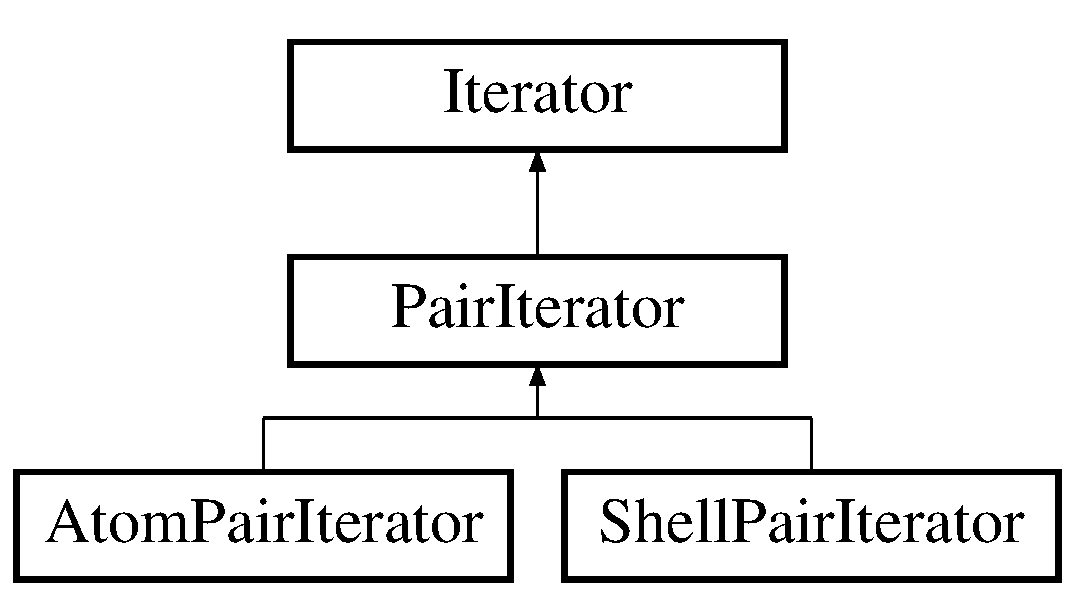
\includegraphics[height=3cm]{classJKBuilder_1_1PairIterator}
\end{center}
\end{figure}
\subsection*{Public Member Functions}
\begin{DoxyCompactItemize}
\item 
int \hyperlink{classJKBuilder_1_1PairIterator_a370ad37c854fbbf6421ebf9ab35cd027}{ID} (const int i) const 
\begin{DoxyCompactList}\small\item\em Returns the ID of element i of the pair. \item\end{DoxyCompactList}\item 
virtual \hyperlink{classJKBuilder_1_1PairIterator_a129fcb5bc5ef5ddd5760925e80573483}{$\sim$PairIterator} ()
\begin{DoxyCompactList}\small\item\em No memory to free. \item\end{DoxyCompactList}\item 
\hyperlink{classJKBuilder_1_1PairIterator_a4863c44859616a6498bd4447b1e3b056}{PairIterator} (\hyperlink{classJKBuilder_1_1PairIterator}{PairIterator} const \&other)
\item 
\hyperlink{classJKBuilder_1_1PairIterator_a2827cf29cfa8dbb7e254901450b52e5e}{PairIterator} (int $\ast$IDs)
\begin{DoxyCompactList}\small\item\em Sets both absoluteIDS to 0. \item\end{DoxyCompactList}\item 
virtual bool \hyperlink{classJKBuilder_1_1PairIterator_a1984297ca1081efc0513ec2f5e6a6177}{operator$<$} (\hyperlink{classJKBuilder_1_1PairIterator}{PairIterator} const \&other)
\item 
bool \hyperlink{classJKBuilder_1_1PairIterator_a9c95b8dd7929cb34336a944ce96e88a7}{operator$<$=} (\hyperlink{classJKBuilder_1_1PairIterator}{PairIterator} const \&other)
\begin{DoxyCompactList}\small\item\em Returns true if operator$<$ is true or operator== is true. \item\end{DoxyCompactList}\item 
bool \hyperlink{classJKBuilder_1_1PairIterator_ab37a738406950a5e19931f4c09b41f29}{operator$>$} (\hyperlink{classJKBuilder_1_1PairIterator}{PairIterator} const \&other)
\begin{DoxyCompactList}\small\item\em Returns true if operator$<$= is false. \item\end{DoxyCompactList}\item 
bool \hyperlink{classJKBuilder_1_1PairIterator_a0064337d38b8f97d0367be2e9bd31d62}{operator$>$=} (\hyperlink{classJKBuilder_1_1PairIterator}{PairIterator} const \&other)
\begin{DoxyCompactList}\small\item\em Returns true if operator$>$ or operator== is true. \item\end{DoxyCompactList}\item 
bool \hyperlink{classJKBuilder_1_1PairIterator_a6b4e430066f478e5e400edd39ef93968}{operator==} (\hyperlink{classJKBuilder_1_1PairIterator}{PairIterator} const \&other) const 
\item 
\hyperlink{classJKBuilder_1_1PairIterator}{PairIterator} \& \hyperlink{classJKBuilder_1_1PairIterator_a698aa7b3d6495bd74dcff5b93be868a8}{operator=} (\hyperlink{classJKBuilder_1_1PairIterator}{PairIterator} const \&other)
\item 
virtual void \hyperlink{classJKBuilder_1_1Iterator_a34ca36a99b20ae3170babadaffe51ed2}{Start} (int n=0)
\begin{DoxyCompactList}\small\item\em Returns an iterator suitable for starting on iteration n. \item\end{DoxyCompactList}\item 
virtual void \hyperlink{classJKBuilder_1_1Iterator_a5f692b73d2e160450f4617bb75825e11}{End} (int n=-\/1)
\begin{DoxyCompactList}\small\item\em Returns an iterator representing the state of the iterator after n iterations have occured. \item\end{DoxyCompactList}\item 
\hyperlink{classJKBuilder_1_1Iterator}{Iterator} \hyperlink{classJKBuilder_1_1Iterator_ac1702aedba13b4112b891b58dfd78eba}{operator++} (int)
\begin{DoxyCompactList}\small\item\em Increments the iterator after returning it's value. \item\end{DoxyCompactList}\item 
\hyperlink{classJKBuilder_1_1Iterator}{Iterator} \& \hyperlink{classJKBuilder_1_1Iterator_ae1f21c74128a5ef5d1b9de72ceb09be8}{operator++} ()
\begin{DoxyCompactList}\small\item\em Increments the iterator before returning it's value. \item\end{DoxyCompactList}\item 
bool \hyperlink{classJKBuilder_1_1Iterator_a8c06af8ae0d9d1614ae9f81629275926}{operator!=} (const \hyperlink{classJKBuilder_1_1Iterator}{Iterator} \&other)
\begin{DoxyCompactList}\small\item\em Returns the opposite of operator==. \item\end{DoxyCompactList}\item 
void \hyperlink{classJKBuilder_1_1Iterator_aa83de505e29125c1d3ac7bb1b13ca15a}{SetStart} (std::vector$<$ int $>$ const \&other)
\begin{DoxyCompactList}\small\item\em Sets the N Indices to the N given in other. \item\end{DoxyCompactList}\item 
void \hyperlink{classJKBuilder_1_1Iterator_aad84ec668b5f41210db34c540aaa31fc}{SetEnd} (std::vector$<$ int $>$ const \&other)
\begin{DoxyCompactList}\small\item\em Sets the N MaxInd in other. \item\end{DoxyCompactList}\item 
int \hyperlink{classJKBuilder_1_1Iterator_a74247cf730a06b23fcb1ec64e5596b25}{operator\mbox{[}$\,$\mbox{]}} (const int i) const 
\begin{DoxyCompactList}\small\item\em Returns index i. \item\end{DoxyCompactList}\end{DoxyCompactItemize}
\subsection*{Protected Member Functions}
\begin{DoxyCompactItemize}
\item 
virtual void \hyperlink{classJKBuilder_1_1PairIterator_a7874a07e98b52f4f147cde6f39353bae}{Iterate} ()
\begin{DoxyCompactList}\small\item\em Returns the next valid pair. \item\end{DoxyCompactList}\end{DoxyCompactItemize}
\subsection*{Protected Attributes}
\begin{DoxyCompactItemize}
\item 
int \hyperlink{classJKBuilder_1_1PairIterator_a5c96d22e39dea8044c7caf8c1213e813}{AbsoluteIDs} \mbox{[}2\mbox{]}
\begin{DoxyCompactList}\small\item\em The absolute identity of the system this pair is part of. \item\end{DoxyCompactList}\item 
std::vector$<$ int $>$ \hyperlink{classJKBuilder_1_1Iterator_a20ca24f6d827aba144bb087c4bcb74a0}{CurrentValue}
\begin{DoxyCompactList}\small\item\em The current value. \item\end{DoxyCompactList}\item 
std::vector$<$ int $>$ \hyperlink{classJKBuilder_1_1Iterator_ab6b56d3c4e9353bc938dd6249cde9ca0}{MaxInd}
\begin{DoxyCompactList}\small\item\em This is a vector of length N containing the maximum each index can be. \item\end{DoxyCompactList}\end{DoxyCompactItemize}
\subsection*{Private Member Functions}
\begin{DoxyCompactItemize}
\item 
void \hyperlink{classJKBuilder_1_1PairIterator_ad9163efc0e961126baecc84da6555045}{Copy} (\hyperlink{classJKBuilder_1_1PairIterator}{PairIterator} const \&other)
\end{DoxyCompactItemize}


\subsection{Detailed Description}
Generalization of \hyperlink{classJKBuilder_1_1Iterator}{Iterator} to a pair iterator that demands that index 0$>$=index 1, as is needed for many pairs. 

\subsection{Constructor \& Destructor Documentation}
\hypertarget{classJKBuilder_1_1PairIterator_a129fcb5bc5ef5ddd5760925e80573483}{
\index{JKBuilder::PairIterator@{JKBuilder::PairIterator}!$\sim$PairIterator@{$\sim$PairIterator}}
\index{$\sim$PairIterator@{$\sim$PairIterator}!JKBuilder::PairIterator@{JKBuilder::PairIterator}}
\subsubsection[{$\sim$PairIterator}]{\setlength{\rightskip}{0pt plus 5cm}$\sim${\bf PairIterator} ()\hspace{0.3cm}{\ttfamily  \mbox{[}virtual\mbox{]}}}}
\label{classJKBuilder_1_1PairIterator_a129fcb5bc5ef5ddd5760925e80573483}


No memory to free. \hypertarget{classJKBuilder_1_1PairIterator_a4863c44859616a6498bd4447b1e3b056}{
\index{JKBuilder::PairIterator@{JKBuilder::PairIterator}!PairIterator@{PairIterator}}
\index{PairIterator@{PairIterator}!JKBuilder::PairIterator@{JKBuilder::PairIterator}}
\subsubsection[{PairIterator}]{\setlength{\rightskip}{0pt plus 5cm}{\bf PairIterator} ({\bf PairIterator} const \& {\em other})}}
\label{classJKBuilder_1_1PairIterator_a4863c44859616a6498bd4447b1e3b056}
\hypertarget{classJKBuilder_1_1PairIterator_a2827cf29cfa8dbb7e254901450b52e5e}{
\index{JKBuilder::PairIterator@{JKBuilder::PairIterator}!PairIterator@{PairIterator}}
\index{PairIterator@{PairIterator}!JKBuilder::PairIterator@{JKBuilder::PairIterator}}
\subsubsection[{PairIterator}]{\setlength{\rightskip}{0pt plus 5cm}{\bf PairIterator} (int $\ast$ {\em IDs} = {\ttfamily NULL})}}
\label{classJKBuilder_1_1PairIterator_a2827cf29cfa8dbb7e254901450b52e5e}


Sets both absoluteIDS to 0. 

\subsection{Member Function Documentation}
\hypertarget{classJKBuilder_1_1PairIterator_ad9163efc0e961126baecc84da6555045}{
\index{JKBuilder::PairIterator@{JKBuilder::PairIterator}!Copy@{Copy}}
\index{Copy@{Copy}!JKBuilder::PairIterator@{JKBuilder::PairIterator}}
\subsubsection[{Copy}]{\setlength{\rightskip}{0pt plus 5cm}void Copy ({\bf PairIterator} const \& {\em other})\hspace{0.3cm}{\ttfamily  \mbox{[}private\mbox{]}}}}
\label{classJKBuilder_1_1PairIterator_ad9163efc0e961126baecc84da6555045}


Reimplemented from \hyperlink{classJKBuilder_1_1Iterator_aacb7559eb1b8aab6e7bb6a56602d97ff}{Iterator}.\hypertarget{classJKBuilder_1_1PairIterator_a7874a07e98b52f4f147cde6f39353bae}{
\index{JKBuilder::PairIterator@{JKBuilder::PairIterator}!Iterate@{Iterate}}
\index{Iterate@{Iterate}!JKBuilder::PairIterator@{JKBuilder::PairIterator}}
\subsubsection[{Iterate}]{\setlength{\rightskip}{0pt plus 5cm}void Iterate ()\hspace{0.3cm}{\ttfamily  \mbox{[}protected, virtual\mbox{]}}}}
\label{classJKBuilder_1_1PairIterator_a7874a07e98b52f4f147cde6f39353bae}


Returns the next valid pair. Letting the indices in this pair be P and Q. This returns the next pair that satisfies Q$<$=P 

Reimplemented from \hyperlink{classJKBuilder_1_1Iterator_a7874a07e98b52f4f147cde6f39353bae}{Iterator}.

Reimplemented in \hyperlink{classJKBuilder_1_1ShellPairIterator_a7874a07e98b52f4f147cde6f39353bae}{ShellPairIterator}.\hypertarget{classJKBuilder_1_1PairIterator_a370ad37c854fbbf6421ebf9ab35cd027}{
\index{JKBuilder::PairIterator@{JKBuilder::PairIterator}!ID@{ID}}
\index{ID@{ID}!JKBuilder::PairIterator@{JKBuilder::PairIterator}}
\subsubsection[{ID}]{\setlength{\rightskip}{0pt plus 5cm}int ID (const int {\em i}) const}}
\label{classJKBuilder_1_1PairIterator_a370ad37c854fbbf6421ebf9ab35cd027}


Returns the ID of element i of the pair. \hypertarget{classJKBuilder_1_1PairIterator_a1984297ca1081efc0513ec2f5e6a6177}{
\index{JKBuilder::PairIterator@{JKBuilder::PairIterator}!operator$<$@{operator$<$}}
\index{operator$<$@{operator$<$}!JKBuilder::PairIterator@{JKBuilder::PairIterator}}
\subsubsection[{operator$<$}]{\setlength{\rightskip}{0pt plus 5cm}bool operator$<$ ({\bf PairIterator} const \& {\em other})\hspace{0.3cm}{\ttfamily  \mbox{[}virtual\mbox{]}}}}
\label{classJKBuilder_1_1PairIterator_a1984297ca1081efc0513ec2f5e6a6177}
\hypertarget{classJKBuilder_1_1PairIterator_a9c95b8dd7929cb34336a944ce96e88a7}{
\index{JKBuilder::PairIterator@{JKBuilder::PairIterator}!operator$<$=@{operator$<$=}}
\index{operator$<$=@{operator$<$=}!JKBuilder::PairIterator@{JKBuilder::PairIterator}}
\subsubsection[{operator$<$=}]{\setlength{\rightskip}{0pt plus 5cm}bool operator$<$= ({\bf PairIterator} const \& {\em other})}}
\label{classJKBuilder_1_1PairIterator_a9c95b8dd7929cb34336a944ce96e88a7}


Returns true if operator$<$ is true or operator== is true. \hypertarget{classJKBuilder_1_1PairIterator_ab37a738406950a5e19931f4c09b41f29}{
\index{JKBuilder::PairIterator@{JKBuilder::PairIterator}!operator$>$@{operator$>$}}
\index{operator$>$@{operator$>$}!JKBuilder::PairIterator@{JKBuilder::PairIterator}}
\subsubsection[{operator$>$}]{\setlength{\rightskip}{0pt plus 5cm}bool operator$>$ ({\bf PairIterator} const \& {\em other})}}
\label{classJKBuilder_1_1PairIterator_ab37a738406950a5e19931f4c09b41f29}


Returns true if operator$<$= is false. \hypertarget{classJKBuilder_1_1PairIterator_a0064337d38b8f97d0367be2e9bd31d62}{
\index{JKBuilder::PairIterator@{JKBuilder::PairIterator}!operator$>$=@{operator$>$=}}
\index{operator$>$=@{operator$>$=}!JKBuilder::PairIterator@{JKBuilder::PairIterator}}
\subsubsection[{operator$>$=}]{\setlength{\rightskip}{0pt plus 5cm}bool operator$>$= ({\bf PairIterator} const \& {\em other})}}
\label{classJKBuilder_1_1PairIterator_a0064337d38b8f97d0367be2e9bd31d62}


Returns true if operator$>$ or operator== is true. \hypertarget{classJKBuilder_1_1PairIterator_a6b4e430066f478e5e400edd39ef93968}{
\index{JKBuilder::PairIterator@{JKBuilder::PairIterator}!operator==@{operator==}}
\index{operator==@{operator==}!JKBuilder::PairIterator@{JKBuilder::PairIterator}}
\subsubsection[{operator==}]{\setlength{\rightskip}{0pt plus 5cm}bool operator== ({\bf PairIterator} const \& {\em other}) const}}
\label{classJKBuilder_1_1PairIterator_a6b4e430066f478e5e400edd39ef93968}


Reimplemented from \hyperlink{classJKBuilder_1_1Iterator_a1ea001976a5bc8ae8dc365e2a912b59a}{Iterator}.\hypertarget{classJKBuilder_1_1PairIterator_a698aa7b3d6495bd74dcff5b93be868a8}{
\index{JKBuilder::PairIterator@{JKBuilder::PairIterator}!operator=@{operator=}}
\index{operator=@{operator=}!JKBuilder::PairIterator@{JKBuilder::PairIterator}}
\subsubsection[{operator=}]{\setlength{\rightskip}{0pt plus 5cm}{\bf PairIterator} \& operator= ({\bf PairIterator} const \& {\em other})}}
\label{classJKBuilder_1_1PairIterator_a698aa7b3d6495bd74dcff5b93be868a8}


Reimplemented from \hyperlink{classJKBuilder_1_1Iterator_ae6f4f24e1855d2aaf89a8a60a9f1521b}{Iterator}.

Reimplemented in \hyperlink{classJKBuilder_1_1AtomPairIterator_aefda578091b26523e72740cec884aa45}{AtomPairIterator}, and \hyperlink{classJKBuilder_1_1ShellPairIterator_af3001050bade3a939d83971d1a3f47e7}{ShellPairIterator}.\hypertarget{classJKBuilder_1_1Iterator_a34ca36a99b20ae3170babadaffe51ed2}{
\index{JKBuilder::PairIterator@{JKBuilder::PairIterator}!Start@{Start}}
\index{Start@{Start}!JKBuilder::PairIterator@{JKBuilder::PairIterator}}
\subsubsection[{Start}]{\setlength{\rightskip}{0pt plus 5cm}void Start (int {\em n} = {\ttfamily 0})\hspace{0.3cm}{\ttfamily  \mbox{[}virtual, inherited\mbox{]}}}}
\label{classJKBuilder_1_1Iterator_a34ca36a99b20ae3170babadaffe51ed2}


Returns an iterator suitable for starting on iteration n. 

Reimplemented in \hyperlink{classJKBuilder_1_1QuartetIterator_a34ca36a99b20ae3170babadaffe51ed2}{QuartetIterator}.\hypertarget{classJKBuilder_1_1Iterator_a5f692b73d2e160450f4617bb75825e11}{
\index{JKBuilder::PairIterator@{JKBuilder::PairIterator}!End@{End}}
\index{End@{End}!JKBuilder::PairIterator@{JKBuilder::PairIterator}}
\subsubsection[{End}]{\setlength{\rightskip}{0pt plus 5cm}void End (int {\em n} = {\ttfamily -\/1})\hspace{0.3cm}{\ttfamily  \mbox{[}virtual, inherited\mbox{]}}}}
\label{classJKBuilder_1_1Iterator_a5f692b73d2e160450f4617bb75825e11}


Returns an iterator representing the state of the iterator after n iterations have occured. The default argument is n=-\/1, which is a flag corresponding to the last iteration of the iterator 

Reimplemented in \hyperlink{classJKBuilder_1_1QuartetIterator_a5f692b73d2e160450f4617bb75825e11}{QuartetIterator}.\hypertarget{classJKBuilder_1_1Iterator_ac1702aedba13b4112b891b58dfd78eba}{
\index{JKBuilder::PairIterator@{JKBuilder::PairIterator}!operator++@{operator++}}
\index{operator++@{operator++}!JKBuilder::PairIterator@{JKBuilder::PairIterator}}
\subsubsection[{operator++}]{\setlength{\rightskip}{0pt plus 5cm}{\bf Iterator} operator++ (int)\hspace{0.3cm}{\ttfamily  \mbox{[}inherited\mbox{]}}}}
\label{classJKBuilder_1_1Iterator_ac1702aedba13b4112b891b58dfd78eba}


Increments the iterator after returning it's value. \hypertarget{classJKBuilder_1_1Iterator_ae1f21c74128a5ef5d1b9de72ceb09be8}{
\index{JKBuilder::PairIterator@{JKBuilder::PairIterator}!operator++@{operator++}}
\index{operator++@{operator++}!JKBuilder::PairIterator@{JKBuilder::PairIterator}}
\subsubsection[{operator++}]{\setlength{\rightskip}{0pt plus 5cm}{\bf Iterator} \& operator++ ()\hspace{0.3cm}{\ttfamily  \mbox{[}inherited\mbox{]}}}}
\label{classJKBuilder_1_1Iterator_ae1f21c74128a5ef5d1b9de72ceb09be8}


Increments the iterator before returning it's value. \hypertarget{classJKBuilder_1_1Iterator_a8c06af8ae0d9d1614ae9f81629275926}{
\index{JKBuilder::PairIterator@{JKBuilder::PairIterator}!operator!=@{operator!=}}
\index{operator!=@{operator!=}!JKBuilder::PairIterator@{JKBuilder::PairIterator}}
\subsubsection[{operator!=}]{\setlength{\rightskip}{0pt plus 5cm}bool operator!= (const {\bf Iterator} \& {\em other})\hspace{0.3cm}{\ttfamily  \mbox{[}inherited\mbox{]}}}}
\label{classJKBuilder_1_1Iterator_a8c06af8ae0d9d1614ae9f81629275926}


Returns the opposite of operator==. \hypertarget{classJKBuilder_1_1Iterator_aa83de505e29125c1d3ac7bb1b13ca15a}{
\index{JKBuilder::PairIterator@{JKBuilder::PairIterator}!SetStart@{SetStart}}
\index{SetStart@{SetStart}!JKBuilder::PairIterator@{JKBuilder::PairIterator}}
\subsubsection[{SetStart}]{\setlength{\rightskip}{0pt plus 5cm}void SetStart (std::vector$<$ int $>$ const \& {\em other})\hspace{0.3cm}{\ttfamily  \mbox{[}inherited\mbox{]}}}}
\label{classJKBuilder_1_1Iterator_aa83de505e29125c1d3ac7bb1b13ca15a}


Sets the N Indices to the N given in other. \hypertarget{classJKBuilder_1_1Iterator_aad84ec668b5f41210db34c540aaa31fc}{
\index{JKBuilder::PairIterator@{JKBuilder::PairIterator}!SetEnd@{SetEnd}}
\index{SetEnd@{SetEnd}!JKBuilder::PairIterator@{JKBuilder::PairIterator}}
\subsubsection[{SetEnd}]{\setlength{\rightskip}{0pt plus 5cm}void SetEnd (std::vector$<$ int $>$ const \& {\em other})\hspace{0.3cm}{\ttfamily  \mbox{[}inherited\mbox{]}}}}
\label{classJKBuilder_1_1Iterator_aad84ec668b5f41210db34c540aaa31fc}


Sets the N MaxInd in other. \hypertarget{classJKBuilder_1_1Iterator_a74247cf730a06b23fcb1ec64e5596b25}{
\index{JKBuilder::PairIterator@{JKBuilder::PairIterator}!operator\mbox{[}\mbox{]}@{operator[]}}
\index{operator\mbox{[}\mbox{]}@{operator[]}!JKBuilder::PairIterator@{JKBuilder::PairIterator}}
\subsubsection[{operator[]}]{\setlength{\rightskip}{0pt plus 5cm}int operator\mbox{[}$\,$\mbox{]} (const int {\em i}) const\hspace{0.3cm}{\ttfamily  \mbox{[}inherited\mbox{]}}}}
\label{classJKBuilder_1_1Iterator_a74247cf730a06b23fcb1ec64e5596b25}


Returns index i. 

\subsection{Member Data Documentation}
\hypertarget{classJKBuilder_1_1PairIterator_a5c96d22e39dea8044c7caf8c1213e813}{
\index{JKBuilder::PairIterator@{JKBuilder::PairIterator}!AbsoluteIDs@{AbsoluteIDs}}
\index{AbsoluteIDs@{AbsoluteIDs}!JKBuilder::PairIterator@{JKBuilder::PairIterator}}
\subsubsection[{AbsoluteIDs}]{\setlength{\rightskip}{0pt plus 5cm}int {\bf AbsoluteIDs}\mbox{[}2\mbox{]}\hspace{0.3cm}{\ttfamily  \mbox{[}protected\mbox{]}}}}
\label{classJKBuilder_1_1PairIterator_a5c96d22e39dea8044c7caf8c1213e813}


The absolute identity of the system this pair is part of. If this is a pair of atoms set all elements of this to 0 (all atoms are part of the same molecule. If this is a pair of shells set it to the identity of the \hyperlink{classJKBuilder_1_1atom}{atom} the shell is on. \hypertarget{classJKBuilder_1_1Iterator_a20ca24f6d827aba144bb087c4bcb74a0}{
\index{JKBuilder::PairIterator@{JKBuilder::PairIterator}!CurrentValue@{CurrentValue}}
\index{CurrentValue@{CurrentValue}!JKBuilder::PairIterator@{JKBuilder::PairIterator}}
\subsubsection[{CurrentValue}]{\setlength{\rightskip}{0pt plus 5cm}std::vector$<$int$>$ {\bf CurrentValue}\hspace{0.3cm}{\ttfamily  \mbox{[}protected, inherited\mbox{]}}}}
\label{classJKBuilder_1_1Iterator_a20ca24f6d827aba144bb087c4bcb74a0}


The current value. \hypertarget{classJKBuilder_1_1Iterator_ab6b56d3c4e9353bc938dd6249cde9ca0}{
\index{JKBuilder::PairIterator@{JKBuilder::PairIterator}!MaxInd@{MaxInd}}
\index{MaxInd@{MaxInd}!JKBuilder::PairIterator@{JKBuilder::PairIterator}}
\subsubsection[{MaxInd}]{\setlength{\rightskip}{0pt plus 5cm}std::vector$<$int$>$ {\bf MaxInd}\hspace{0.3cm}{\ttfamily  \mbox{[}protected, inherited\mbox{]}}}}
\label{classJKBuilder_1_1Iterator_ab6b56d3c4e9353bc938dd6249cde9ca0}


This is a vector of length N containing the maximum each index can be. 

The documentation for this class was generated from the following files:\begin{DoxyCompactItemize}
\item 
src/\hyperlink{Iterators_8h}{Iterators.h}\item 
src/\hyperlink{Iterator_8cpp}{Iterator.cpp}\end{DoxyCompactItemize}

\hypertarget{classJKBuilder_1_1Primitive}{
\section{Primitive Class Reference}
\label{classJKBuilder_1_1Primitive}\index{JKBuilder::Primitive@{JKBuilder::Primitive}}
}


A Gaussian primitive.  


{\ttfamily \#include $<$BasisSet.h$>$}\subsection*{Public Member Functions}
\begin{DoxyCompactItemize}
\item 
\hyperlink{classJKBuilder_1_1Primitive_ad5c80a16eab14367b76a4dc79844d0d5}{Primitive} (double c0=0, double beta0=0)
\begin{DoxyCompactList}\small\item\em Creates a \hyperlink{classJKBuilder_1_1Primitive}{Primitive} with exponent scale factor beta0 and expansion coefficient c0. \item\end{DoxyCompactList}\item 
double \hyperlink{classJKBuilder_1_1Primitive_a229a18fdc499aafe149c55011f9fb2fb}{GetC} ()
\begin{DoxyCompactList}\small\item\em Returns c. \item\end{DoxyCompactList}\item 
double \hyperlink{classJKBuilder_1_1Primitive_a8b788f95c3fa1f2cc9aedaa1b92b78a1}{GetBeta} ()
\begin{DoxyCompactList}\small\item\em Returns beta. \item\end{DoxyCompactList}\item 
void \hyperlink{classJKBuilder_1_1Primitive_a388f572c62279f839ee138a9afbdeeb5}{print} ()
\begin{DoxyCompactList}\small\item\em Prints out the primitive. \item\end{DoxyCompactList}\end{DoxyCompactItemize}
\subsection*{Private Attributes}
\begin{DoxyCompactItemize}
\item 
double \hyperlink{classJKBuilder_1_1Primitive_a2c09e929a6ea340fc9653cca414b11d3}{c}
\begin{DoxyCompactList}\small\item\em The expansion coefficient of this primitive. \item\end{DoxyCompactList}\item 
double \hyperlink{classJKBuilder_1_1Primitive_a9424343761f8c4f4c1afe8f5b6bf471b}{beta}
\begin{DoxyCompactList}\small\item\em The exponent scale factor of this primitive. \item\end{DoxyCompactList}\end{DoxyCompactItemize}


\subsection{Detailed Description}
A Gaussian primitive. Gaussian primitives are assumed of the form:

\[ g_i\left(\bf{r}:c_i,\beta_i\right)=c_i\ \rm{e}^{-\beta_i\bf{r}^2}, \]

where $c_i$ is the expansion coefficient associated with this primitive, and $\beta_i$ is exponent scale factor. The smaller $\beta_i$ the more diffuse the primitive. 

\subsection{Constructor \& Destructor Documentation}
\hypertarget{classJKBuilder_1_1Primitive_ad5c80a16eab14367b76a4dc79844d0d5}{
\index{JKBuilder::Primitive@{JKBuilder::Primitive}!Primitive@{Primitive}}
\index{Primitive@{Primitive}!JKBuilder::Primitive@{JKBuilder::Primitive}}
\subsubsection[{Primitive}]{\setlength{\rightskip}{0pt plus 5cm}{\bf Primitive} (double {\em c0} = {\ttfamily 0}, \/  double {\em beta0} = {\ttfamily 0})}}
\label{classJKBuilder_1_1Primitive_ad5c80a16eab14367b76a4dc79844d0d5}


Creates a \hyperlink{classJKBuilder_1_1Primitive}{Primitive} with exponent scale factor beta0 and expansion coefficient c0. 

\subsection{Member Function Documentation}
\hypertarget{classJKBuilder_1_1Primitive_a229a18fdc499aafe149c55011f9fb2fb}{
\index{JKBuilder::Primitive@{JKBuilder::Primitive}!GetC@{GetC}}
\index{GetC@{GetC}!JKBuilder::Primitive@{JKBuilder::Primitive}}
\subsubsection[{GetC}]{\setlength{\rightskip}{0pt plus 5cm}double GetC ()}}
\label{classJKBuilder_1_1Primitive_a229a18fdc499aafe149c55011f9fb2fb}


Returns c. \hypertarget{classJKBuilder_1_1Primitive_a8b788f95c3fa1f2cc9aedaa1b92b78a1}{
\index{JKBuilder::Primitive@{JKBuilder::Primitive}!GetBeta@{GetBeta}}
\index{GetBeta@{GetBeta}!JKBuilder::Primitive@{JKBuilder::Primitive}}
\subsubsection[{GetBeta}]{\setlength{\rightskip}{0pt plus 5cm}double GetBeta ()}}
\label{classJKBuilder_1_1Primitive_a8b788f95c3fa1f2cc9aedaa1b92b78a1}


Returns beta. \hypertarget{classJKBuilder_1_1Primitive_a388f572c62279f839ee138a9afbdeeb5}{
\index{JKBuilder::Primitive@{JKBuilder::Primitive}!print@{print}}
\index{print@{print}!JKBuilder::Primitive@{JKBuilder::Primitive}}
\subsubsection[{print}]{\setlength{\rightskip}{0pt plus 5cm}void print ()}}
\label{classJKBuilder_1_1Primitive_a388f572c62279f839ee138a9afbdeeb5}


Prints out the primitive. 

\subsection{Member Data Documentation}
\hypertarget{classJKBuilder_1_1Primitive_a2c09e929a6ea340fc9653cca414b11d3}{
\index{JKBuilder::Primitive@{JKBuilder::Primitive}!c@{c}}
\index{c@{c}!JKBuilder::Primitive@{JKBuilder::Primitive}}
\subsubsection[{c}]{\setlength{\rightskip}{0pt plus 5cm}double {\bf c}\hspace{0.3cm}{\ttfamily  \mbox{[}private\mbox{]}}}}
\label{classJKBuilder_1_1Primitive_a2c09e929a6ea340fc9653cca414b11d3}


The expansion coefficient of this primitive. \hypertarget{classJKBuilder_1_1Primitive_a9424343761f8c4f4c1afe8f5b6bf471b}{
\index{JKBuilder::Primitive@{JKBuilder::Primitive}!beta@{beta}}
\index{beta@{beta}!JKBuilder::Primitive@{JKBuilder::Primitive}}
\subsubsection[{beta}]{\setlength{\rightskip}{0pt plus 5cm}double {\bf beta}\hspace{0.3cm}{\ttfamily  \mbox{[}private\mbox{]}}}}
\label{classJKBuilder_1_1Primitive_a9424343761f8c4f4c1afe8f5b6bf471b}


The exponent scale factor of this primitive. 

The documentation for this class was generated from the following files:\begin{DoxyCompactItemize}
\item 
src/\hyperlink{BasisSet_8h}{BasisSet.h}\item 
src/\hyperlink{BasisSet_8cpp}{BasisSet.cpp}\end{DoxyCompactItemize}

\hypertarget{classJKBuilder_1_1printer}{
\section{printer Class Reference}
\label{classJKBuilder_1_1printer}\index{JKBuilder::printer@{JKBuilder::printer}}
}


The class in charge of printing to std::cout.  


{\ttfamily \#include $<$printer.h$>$}Inheritance diagram for printer::\begin{figure}[H]
\begin{center}
\leavevmode
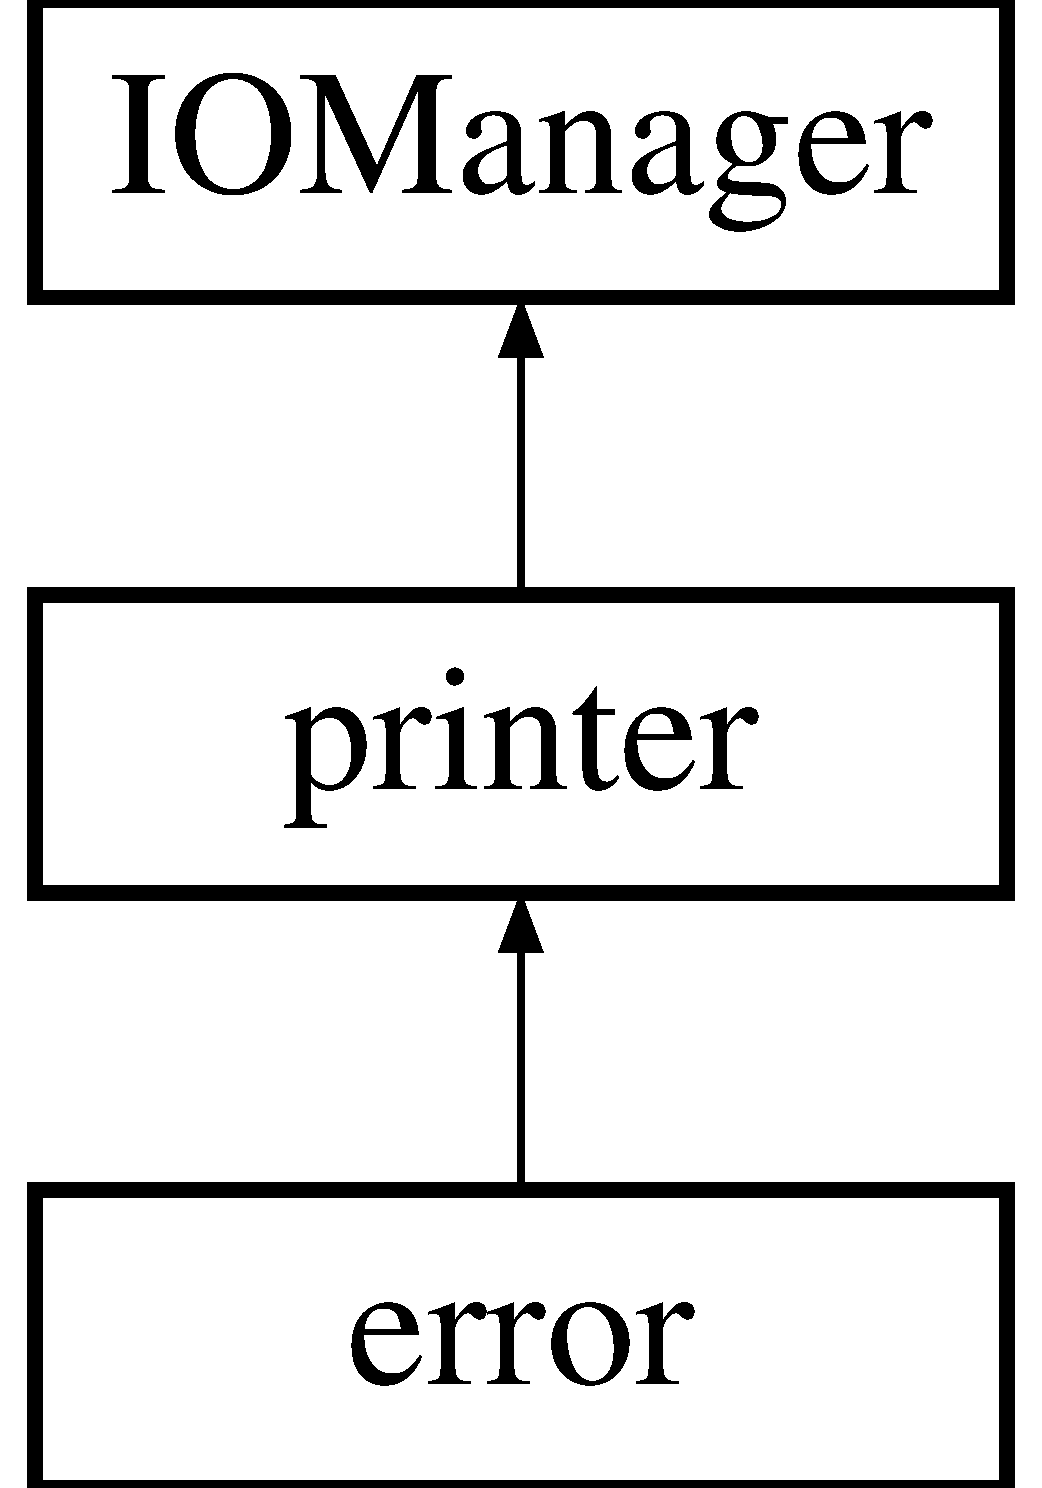
\includegraphics[height=3cm]{classJKBuilder_1_1printer}
\end{center}
\end{figure}
\subsection*{Public Member Functions}
\begin{DoxyCompactItemize}
\item 
\hyperlink{classJKBuilder_1_1printer_af4e2cc2ab8b108895389d46fa14d4a13}{printer} (int ncolumns=80)
\begin{DoxyCompactList}\small\item\em Input is the number of columns we are allowed to print out to, ncolumns defaults to 80. \item\end{DoxyCompactList}\item 
virtual \hyperlink{classJKBuilder_1_1printer_a555702a98f98cda2ba39f19c0c9397c6}{$\sim$printer} ()
\begin{DoxyCompactList}\small\item\em No memory to free so it does nothing. \item\end{DoxyCompactList}\item 
{\footnotesize template$<$class T $>$ }\\\hyperlink{classJKBuilder_1_1IOManager}{IOManager} \& \hyperlink{classJKBuilder_1_1IOManager_a505a35212a21e4884ed24b021c0add4b}{operator$<$$<$} (const T \&message)
\begin{DoxyCompactList}\small\item\em This is the call that prints our messages, unless it is a double... \item\end{DoxyCompactList}\item 
\hyperlink{classJKBuilder_1_1IOManager}{IOManager} \& \hyperlink{classJKBuilder_1_1IOManager_a127779d1803b6ffe9e44a3a36e46910e}{operator$<$$<$} (const double \&message)
\begin{DoxyCompactList}\small\item\em Then it is this call, because we want to control the precision then. \item\end{DoxyCompactList}\item 
\hyperlink{classJKBuilder_1_1IOManager}{IOManager} \& \hyperlink{classJKBuilder_1_1IOManager_a4ab394f377d37c6598659317320ec38c}{operator$<$$<$} (std::ostream \&($\ast$fn)(std::ostream \&))
\begin{DoxyCompactList}\small\item\em This function is used for the endl character. \item\end{DoxyCompactList}\end{DoxyCompactItemize}
\subsection*{Static Public Attributes}
\begin{DoxyCompactItemize}
\item 
static bool \hyperlink{classJKBuilder_1_1IOManager_aababa9aef0d20ddcfce2d78f41ae1dd8}{power} = true
\begin{DoxyCompactList}\small\item\em The state of the printer's power. \item\end{DoxyCompactList}\end{DoxyCompactItemize}
\subsection*{Protected Member Functions}
\begin{DoxyCompactItemize}
\item 
virtual void \hyperlink{classJKBuilder_1_1printer_a7f207ac705d33a0cd9794a9f0b4a1fa0}{EoL} ()
\begin{DoxyCompactList}\small\item\em Returns the End of Line character, this form also resets the column. \item\end{DoxyCompactList}\item 
void \hyperlink{classJKBuilder_1_1printer_aa32ee0a81ade611982bfc9861c5a05bb}{print} (const string message)
\begin{DoxyCompactList}\small\item\em This is the function that actually does the printing. \item\end{DoxyCompactList}\end{DoxyCompactItemize}
\subsection*{Protected Attributes}
\begin{DoxyCompactItemize}
\item 
std::stringstream \hyperlink{classJKBuilder_1_1IOManager_adbf6a7492c6521b38c1510aebe307770}{buffer}
\begin{DoxyCompactList}\small\item\em This is the line/data we want to print out. \item\end{DoxyCompactList}\item 
std::ostream $\ast$ \hyperlink{classJKBuilder_1_1IOManager_aafe3b1218427d92a689d147f74e74f4b}{Output}
\begin{DoxyCompactList}\small\item\em Returns the current output, defaults to cout. \item\end{DoxyCompactList}\item 
int \hyperlink{classJKBuilder_1_1IOManager_aa95455ed52a8459fad69509a4a0411b5}{precision}
\begin{DoxyCompactList}\small\item\em The precision a double will be printed to. \item\end{DoxyCompactList}\end{DoxyCompactItemize}
\subsection*{Private Attributes}
\begin{DoxyCompactItemize}
\item 
int \hyperlink{classJKBuilder_1_1printer_a7c4b990ebe8d2c098f3974f6ffe0c9b4}{ncols}
\begin{DoxyCompactList}\small\item\em The number of columns we are allowed to print out to before word wrap. \item\end{DoxyCompactList}\end{DoxyCompactItemize}
\subsection*{Static Private Attributes}
\begin{DoxyCompactItemize}
\item 
static int \hyperlink{classJKBuilder_1_1printer_a60dae4c6e78188cd718b696e4f08fc71}{column} = 0
\begin{DoxyCompactList}\small\item\em This is which of the ncols we are printing to. \item\end{DoxyCompactList}\end{DoxyCompactItemize}


\subsection{Detailed Description}
The class in charge of printing to std::cout. As the name of the class implies, this class is designed to handle all of my printing. It's biggest feature is come release time, I can pull the plug on all printers, simultaneously by shutting off the power and I will never see printing from this library again. 

\subsection{Constructor \& Destructor Documentation}
\hypertarget{classJKBuilder_1_1printer_af4e2cc2ab8b108895389d46fa14d4a13}{
\index{JKBuilder::printer@{JKBuilder::printer}!printer@{printer}}
\index{printer@{printer}!JKBuilder::printer@{JKBuilder::printer}}
\subsubsection[{printer}]{\setlength{\rightskip}{0pt plus 5cm}{\bf printer} (int {\em ncolumns} = {\ttfamily 80})}}
\label{classJKBuilder_1_1printer_af4e2cc2ab8b108895389d46fa14d4a13}


Input is the number of columns we are allowed to print out to, ncolumns defaults to 80. \hypertarget{classJKBuilder_1_1printer_a555702a98f98cda2ba39f19c0c9397c6}{
\index{JKBuilder::printer@{JKBuilder::printer}!$\sim$printer@{$\sim$printer}}
\index{$\sim$printer@{$\sim$printer}!JKBuilder::printer@{JKBuilder::printer}}
\subsubsection[{$\sim$printer}]{\setlength{\rightskip}{0pt plus 5cm}$\sim${\bf printer} ()\hspace{0.3cm}{\ttfamily  \mbox{[}virtual\mbox{]}}}}
\label{classJKBuilder_1_1printer_a555702a98f98cda2ba39f19c0c9397c6}


No memory to free so it does nothing. 

\subsection{Member Function Documentation}
\hypertarget{classJKBuilder_1_1printer_a7f207ac705d33a0cd9794a9f0b4a1fa0}{
\index{JKBuilder::printer@{JKBuilder::printer}!EoL@{EoL}}
\index{EoL@{EoL}!JKBuilder::printer@{JKBuilder::printer}}
\subsubsection[{EoL}]{\setlength{\rightskip}{0pt plus 5cm}void EoL ()\hspace{0.3cm}{\ttfamily  \mbox{[}protected, virtual\mbox{]}}}}
\label{classJKBuilder_1_1printer_a7f207ac705d33a0cd9794a9f0b4a1fa0}


Returns the End of Line character, this form also resets the column. 

Reimplemented from \hyperlink{classJKBuilder_1_1IOManager_a7f207ac705d33a0cd9794a9f0b4a1fa0}{IOManager}.

Reimplemented in \hyperlink{classJKBuilder_1_1error_a7f207ac705d33a0cd9794a9f0b4a1fa0}{error}.\hypertarget{classJKBuilder_1_1printer_aa32ee0a81ade611982bfc9861c5a05bb}{
\index{JKBuilder::printer@{JKBuilder::printer}!print@{print}}
\index{print@{print}!JKBuilder::printer@{JKBuilder::printer}}
\subsubsection[{print}]{\setlength{\rightskip}{0pt plus 5cm}void print (const string {\em message})\hspace{0.3cm}{\ttfamily  \mbox{[}protected, virtual\mbox{]}}}}
\label{classJKBuilder_1_1printer_aa32ee0a81ade611982bfc9861c5a05bb}


This is the function that actually does the printing. 

Reimplemented from \hyperlink{classJKBuilder_1_1IOManager_a3abc9519dd5220ecb1154daa25f557fe}{IOManager}.\hypertarget{classJKBuilder_1_1IOManager_a505a35212a21e4884ed24b021c0add4b}{
\index{JKBuilder::printer@{JKBuilder::printer}!operator$<$$<$@{operator$<$$<$}}
\index{operator$<$$<$@{operator$<$$<$}!JKBuilder::printer@{JKBuilder::printer}}
\subsubsection[{operator$<$$<$}]{\setlength{\rightskip}{0pt plus 5cm}{\bf IOManager} \& operator$<$$<$ (const T \& {\em message})\hspace{0.3cm}{\ttfamily  \mbox{[}inline, inherited\mbox{]}}}}
\label{classJKBuilder_1_1IOManager_a505a35212a21e4884ed24b021c0add4b}


This is the call that prints our messages, unless it is a double... \hypertarget{classJKBuilder_1_1IOManager_a127779d1803b6ffe9e44a3a36e46910e}{
\index{JKBuilder::printer@{JKBuilder::printer}!operator$<$$<$@{operator$<$$<$}}
\index{operator$<$$<$@{operator$<$$<$}!JKBuilder::printer@{JKBuilder::printer}}
\subsubsection[{operator$<$$<$}]{\setlength{\rightskip}{0pt plus 5cm}{\bf IOManager} \& operator$<$$<$ (const double \& {\em message})\hspace{0.3cm}{\ttfamily  \mbox{[}inherited\mbox{]}}}}
\label{classJKBuilder_1_1IOManager_a127779d1803b6ffe9e44a3a36e46910e}


Then it is this call, because we want to control the precision then. \hypertarget{classJKBuilder_1_1IOManager_a4ab394f377d37c6598659317320ec38c}{
\index{JKBuilder::printer@{JKBuilder::printer}!operator$<$$<$@{operator$<$$<$}}
\index{operator$<$$<$@{operator$<$$<$}!JKBuilder::printer@{JKBuilder::printer}}
\subsubsection[{operator$<$$<$}]{\setlength{\rightskip}{0pt plus 5cm}{\bf IOManager} \& operator$<$$<$ (std::ostream \&($\ast$)(std::ostream \&) {\em fn})\hspace{0.3cm}{\ttfamily  \mbox{[}inherited\mbox{]}}}}
\label{classJKBuilder_1_1IOManager_a4ab394f377d37c6598659317320ec38c}


This function is used for the endl character. When invoked with \char`\"{}endl\char`\"{} prints the content of the stringstream and clears it. Supports multiple endl's in a stream. The weird function signature is due to the signature of endl. 

\subsection{Member Data Documentation}
\hypertarget{classJKBuilder_1_1printer_a7c4b990ebe8d2c098f3974f6ffe0c9b4}{
\index{JKBuilder::printer@{JKBuilder::printer}!ncols@{ncols}}
\index{ncols@{ncols}!JKBuilder::printer@{JKBuilder::printer}}
\subsubsection[{ncols}]{\setlength{\rightskip}{0pt plus 5cm}int {\bf ncols}\hspace{0.3cm}{\ttfamily  \mbox{[}private\mbox{]}}}}
\label{classJKBuilder_1_1printer_a7c4b990ebe8d2c098f3974f6ffe0c9b4}


The number of columns we are allowed to print out to before word wrap. \hypertarget{classJKBuilder_1_1printer_a60dae4c6e78188cd718b696e4f08fc71}{
\index{JKBuilder::printer@{JKBuilder::printer}!column@{column}}
\index{column@{column}!JKBuilder::printer@{JKBuilder::printer}}
\subsubsection[{column}]{\setlength{\rightskip}{0pt plus 5cm}int {\bf column} = 0\hspace{0.3cm}{\ttfamily  \mbox{[}static, private\mbox{]}}}}
\label{classJKBuilder_1_1printer_a60dae4c6e78188cd718b696e4f08fc71}


This is which of the ncols we are printing to. \hypertarget{classJKBuilder_1_1IOManager_adbf6a7492c6521b38c1510aebe307770}{
\index{JKBuilder::printer@{JKBuilder::printer}!buffer@{buffer}}
\index{buffer@{buffer}!JKBuilder::printer@{JKBuilder::printer}}
\subsubsection[{buffer}]{\setlength{\rightskip}{0pt plus 5cm}std::stringstream {\bf buffer}\hspace{0.3cm}{\ttfamily  \mbox{[}protected, inherited\mbox{]}}}}
\label{classJKBuilder_1_1IOManager_adbf6a7492c6521b38c1510aebe307770}


This is the line/data we want to print out. \hypertarget{classJKBuilder_1_1IOManager_aafe3b1218427d92a689d147f74e74f4b}{
\index{JKBuilder::printer@{JKBuilder::printer}!Output@{Output}}
\index{Output@{Output}!JKBuilder::printer@{JKBuilder::printer}}
\subsubsection[{Output}]{\setlength{\rightskip}{0pt plus 5cm}std::ostream$\ast$ {\bf Output}\hspace{0.3cm}{\ttfamily  \mbox{[}protected, inherited\mbox{]}}}}
\label{classJKBuilder_1_1IOManager_aafe3b1218427d92a689d147f74e74f4b}


Returns the current output, defaults to cout. \hypertarget{classJKBuilder_1_1IOManager_aa95455ed52a8459fad69509a4a0411b5}{
\index{JKBuilder::printer@{JKBuilder::printer}!precision@{precision}}
\index{precision@{precision}!JKBuilder::printer@{JKBuilder::printer}}
\subsubsection[{precision}]{\setlength{\rightskip}{0pt plus 5cm}int {\bf precision}\hspace{0.3cm}{\ttfamily  \mbox{[}protected, inherited\mbox{]}}}}
\label{classJKBuilder_1_1IOManager_aa95455ed52a8459fad69509a4a0411b5}


The precision a double will be printed to. \hypertarget{classJKBuilder_1_1IOManager_aababa9aef0d20ddcfce2d78f41ae1dd8}{
\index{JKBuilder::printer@{JKBuilder::printer}!power@{power}}
\index{power@{power}!JKBuilder::printer@{JKBuilder::printer}}
\subsubsection[{power}]{\setlength{\rightskip}{0pt plus 5cm}bool {\bf power} = true\hspace{0.3cm}{\ttfamily  \mbox{[}static, inherited\mbox{]}}}}
\label{classJKBuilder_1_1IOManager_aababa9aef0d20ddcfce2d78f41ae1dd8}


The state of the printer's power. If true then we are printing data to the output. If false then we are not. Note the static keyword. Turning off power for one \hyperlink{classJKBuilder_1_1printer}{printer} turns off the power for all of them. You flipped the breaker if you will. 

The documentation for this class was generated from the following files:\begin{DoxyCompactItemize}
\item 
src/\hyperlink{printer_8h}{printer.h}\item 
src/\hyperlink{printer_8cpp}{printer.cpp}\end{DoxyCompactItemize}

\hypertarget{classpsi_1_1scf_1_1Psi4JK}{
\section{Psi4JK Class Reference}
\label{classpsi_1_1scf_1_1Psi4JK}\index{psi::scf::Psi4JK@{psi::scf::Psi4JK}}
}


{\ttfamily \#include $<$Psi4JK.h$>$}Inheritance diagram for Psi4JK::\begin{figure}[H]
\begin{center}
\leavevmode
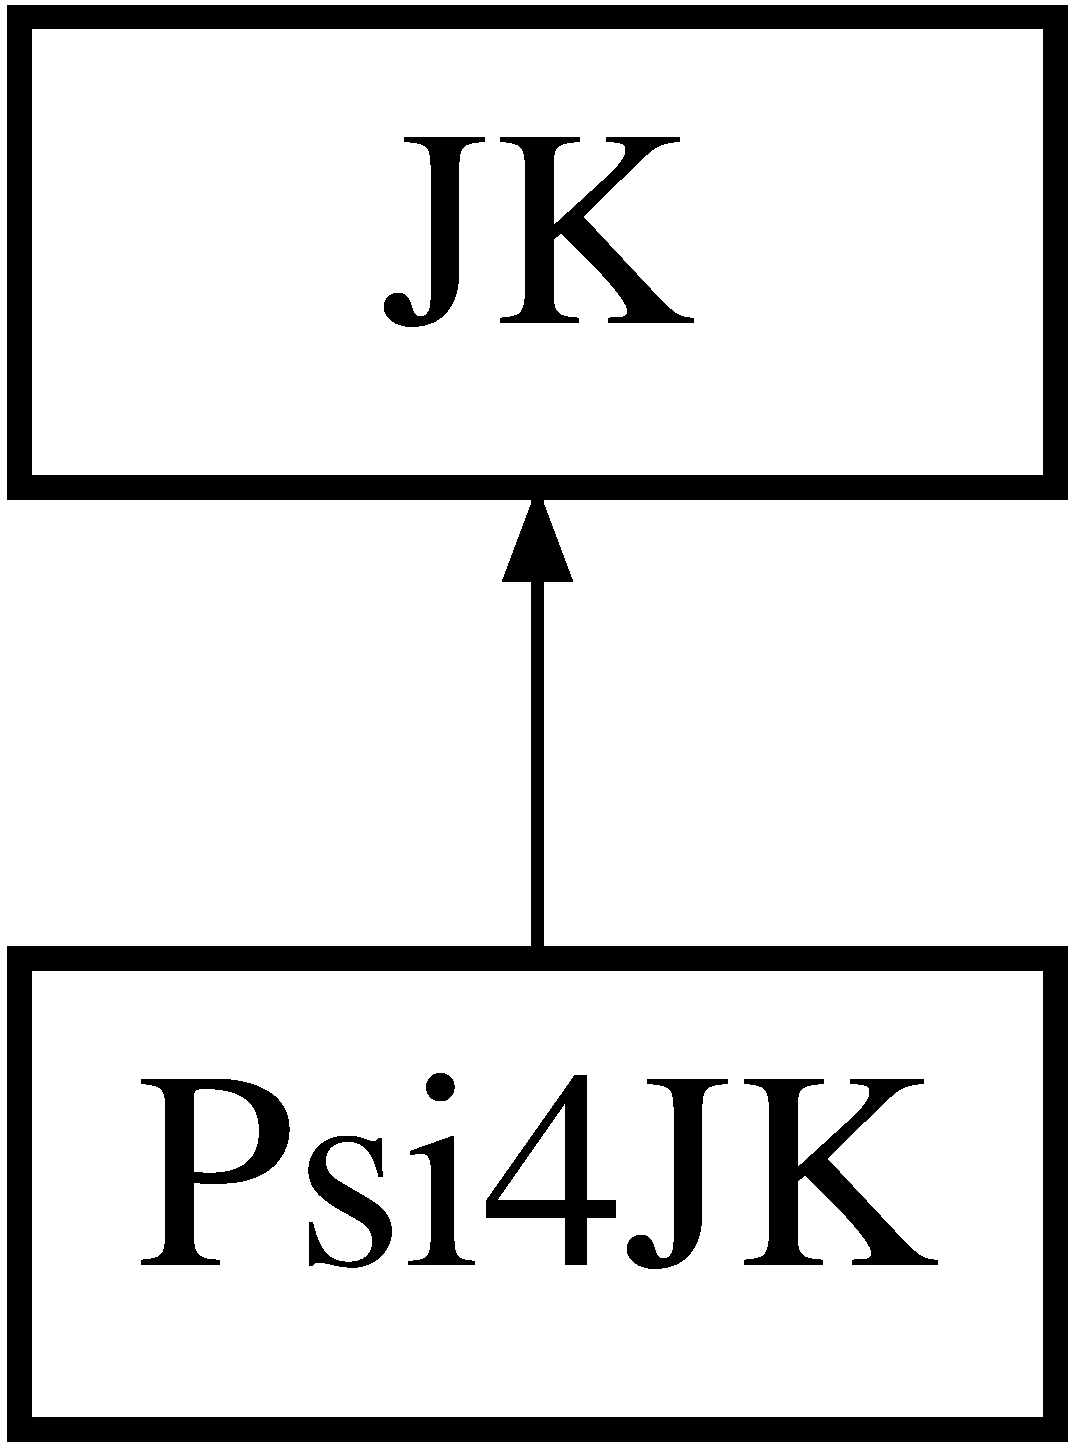
\includegraphics[height=2cm]{classpsi_1_1scf_1_1Psi4JK}
\end{center}
\end{figure}
\subsection*{Public Member Functions}
\begin{DoxyCompactItemize}
\item 
\hyperlink{classpsi_1_1scf_1_1Psi4JK_ad4c73ca14721107f570bbf67a1ce18bb}{Psi4JK} (\hyperlink{namespacepsi_a00b3104f9d454b5adfe2d16e5f8d1e14}{SharedPsiBasis} \&PsiBasis, const \hyperlink{namespacepsi_a672173d36fd5e5d06c17ff19c3bacb9d}{SharedMatrix} \&Density, \hyperlink{namespacepsi_a672173d36fd5e5d06c17ff19c3bacb9d}{SharedMatrix} \&\hyperlink{classJKBuilder_1_1JK_aa04a91cc219b5dabfce19d5316f96887}{J}, \hyperlink{namespacepsi_a672173d36fd5e5d06c17ff19c3bacb9d}{SharedMatrix} \&\hyperlink{classJKBuilder_1_1JK_a5160b673d25f0110d98097f8e7364315}{K})
\item 
void \hyperlink{classpsi_1_1scf_1_1Psi4JK_a36bddec95b737f7ee42688b0de2e730b}{UpdateDensity} (const \hyperlink{namespacepsi_a672173d36fd5e5d06c17ff19c3bacb9d}{SharedMatrix} \&Density, \hyperlink{namespacepsi_a672173d36fd5e5d06c17ff19c3bacb9d}{SharedMatrix} \&\hyperlink{classJKBuilder_1_1JK_aa04a91cc219b5dabfce19d5316f96887}{J}, \hyperlink{namespacepsi_a672173d36fd5e5d06c17ff19c3bacb9d}{SharedMatrix} \&\hyperlink{classJKBuilder_1_1JK_a5160b673d25f0110d98097f8e7364315}{K})
\item 
void \hyperlink{classJKBuilder_1_1JK_ac0b62715458b98f8426017fdd8864670}{UpdateDensity} (const double $\ast$DensityMatrix)
\item 
double $\ast$ \hyperlink{classJKBuilder_1_1JK_ada0787d51feb1496d4aa3a786f870f88}{J\_\-Address} ()
\item 
double $\ast$ \hyperlink{classJKBuilder_1_1JK_a198d3c4da107eb0d9cfafa795f8d635b}{K\_\-Address} ()
\item 
double $\ast$ \hyperlink{classJKBuilder_1_1JK_a5104eb472d984f59df6ca3b91c625209}{Rho} ()
\end{DoxyCompactItemize}
\subsection*{Protected Member Functions}
\begin{DoxyCompactItemize}
\item 
void \hyperlink{classJKBuilder_1_1JK_a13b685265e196c183897777ec2f3136a}{SetUp} (AOBasisSet $\ast$\hyperlink{classJKBuilder_1_1JK_a81392b84b45d3cf84c5c105e9fd5d09c}{basis}, molecule\_\-class $\ast$\hyperlink{classJKBuilder_1_1JK_ad646bdee4fc9f601f954b4a98c4da476}{molecule}, const double $\ast$DensityMatrix, double $\ast$\hyperlink{classJKBuilder_1_1JK_aa04a91cc219b5dabfce19d5316f96887}{J}, double $\ast$\hyperlink{classJKBuilder_1_1JK_a5160b673d25f0110d98097f8e7364315}{K})
\begin{DoxyCompactList}\small\item\em Sets up a bare-\/bones, distributed, \hyperlink{classJKBuilder_1_1JK}{JK} object in the DesiredBasis, on the desired molecule. \item\end{DoxyCompactList}\end{DoxyCompactItemize}
\subsection*{Protected Attributes}
\begin{DoxyCompactItemize}
\item 
bool \hyperlink{classJKBuilder_1_1JK_a072479da68be17a25570325316eade23}{Distributed}
\begin{DoxyCompactList}\small\item\em Are we calling the distributed \hyperlink{classJKBuilder_1_1JK}{JK} Builder, then true. False if we want the shared memory version. \item\end{DoxyCompactList}\item 
bool \hyperlink{classJKBuilder_1_1JK_a6324fcb7d27b80663a26f90a35f2e9b9}{Disk}
\begin{DoxyCompactList}\small\item\em Are we storing stuff on disk (true) or in memory (false). \item\end{DoxyCompactList}\item 
JKFactory $\ast$ \hyperlink{classJKBuilder_1_1JK_a09e4ffeb9ba2c95bf981da66beecc033}{SweatShop}
\begin{DoxyCompactList}\small\item\em Handles all the building of J and K objects. \item\end{DoxyCompactList}\item 
molecule\_\-class $\ast$ \hyperlink{classJKBuilder_1_1JK_ad646bdee4fc9f601f954b4a98c4da476}{molecule}
\item 
std::vector$<$ SharedSymJKMatrix $>$ \hyperlink{classJKBuilder_1_1JK_aa04a91cc219b5dabfce19d5316f96887}{J}
\begin{DoxyCompactList}\small\item\em The J \hyperlink{classJKBuilder_1_1matrix}{matrix}. \item\end{DoxyCompactList}\item 
std::vector$<$ SharedSymJKMatrix $>$ \hyperlink{classJKBuilder_1_1JK_a5160b673d25f0110d98097f8e7364315}{K}
\begin{DoxyCompactList}\small\item\em The K \hyperlink{classJKBuilder_1_1matrix}{matrix}. \item\end{DoxyCompactList}\item 
AOBasisSet $\ast$ \hyperlink{classJKBuilder_1_1JK_a81392b84b45d3cf84c5c105e9fd5d09c}{basis}
\item 
Integrals \hyperlink{classJKBuilder_1_1JK_ad95ede2076c192d856848b3635efc38e}{DaInts}
\end{DoxyCompactItemize}
\subsection*{Private Member Functions}
\begin{DoxyCompactItemize}
\item 
void \hyperlink{classpsi_1_1scf_1_1Psi4JK_a3c559c20a0aa33fa3c6d9bf9e9aefff8}{MakeT} ()
\begin{DoxyCompactList}\small\item\em Function that sets up T. \item\end{DoxyCompactList}\item 
void \hyperlink{classpsi_1_1scf_1_1Psi4JK_a33ac8f638424d92033ec6a72ffc96d6b}{FillBasis} (psi::BasisSet \&PsiBasis)
\begin{DoxyCompactList}\small\item\em Function that makes the \hyperlink{classJKBuilder_1_1AOBasisSet}{JKBuilder::AOBasisSet} object (allocates the memory for it). \item\end{DoxyCompactList}\item 
void \hyperlink{classpsi_1_1scf_1_1Psi4JK_a1cd8cf0f476576f25976b4b822230afa}{MakeMolecule} (psi::BasisSet \&PsiBasis)
\begin{DoxyCompactList}\small\item\em Function that makes the \hyperlink{classJKBuilder_1_1molecule__class}{JKBuilder::molecule\_\-class} object (allocates the memory for it). \item\end{DoxyCompactList}\item 
void \hyperlink{classpsi_1_1scf_1_1Psi4JK_ac2f36c6229344fb608c6d868377a5548}{UpdateJorK} (\hyperlink{namespacepsi_a672173d36fd5e5d06c17ff19c3bacb9d}{SharedMatrix} \&NewMat, \hyperlink{namespaceJKBuilder_aef21bc37b7cf7bc5ebb5a48628db8d0f}{JKBuilder::SharedSymJKMatrix} \&MyMatrix)
\begin{DoxyCompactList}\small\item\em Given a Psi4 matrix, NewMat, builds a SharedSymJKMatrix around the pointer. \item\end{DoxyCompactList}\item 
void \hyperlink{classpsi_1_1scf_1_1Psi4JK_a76433c0bae70a347630890a4c497b488}{MakeInts} (\hyperlink{namespacepsi_a00b3104f9d454b5adfe2d16e5f8d1e14}{SharedPsiBasis} \&PsiBasis)
\end{DoxyCompactItemize}
\subsection*{Private Attributes}
\begin{DoxyCompactItemize}
\item 
double $\ast$ \hyperlink{classpsi_1_1scf_1_1Psi4JK_a92cb38c784d8c2e0b1c80d40e5a2fe64}{density}
\item 
int \hyperlink{classpsi_1_1scf_1_1Psi4JK_a58cb6ef9f81c24f9444912b29a402a7a}{nbasis}
\item 
\hyperlink{namespacepsi_a672173d36fd5e5d06c17ff19c3bacb9d}{SharedMatrix} \hyperlink{classpsi_1_1scf_1_1Psi4JK_af705cc477a1c67061c47a2e881c15422}{T}
\begin{DoxyCompactList}\small\item\em The transformation matrix to ERD's ordering. \item\end{DoxyCompactList}\item 
bool \hyperlink{classpsi_1_1scf_1_1Psi4JK_aff7a60d3f21b50f4ad18e40d99d33a61}{scale}
\begin{DoxyCompactList}\small\item\em True if we need to transform with T. \item\end{DoxyCompactList}\item 
std::vector$<$ \hyperlink{namespacepsi_a7b2115040860b8011075023be6fbeb9a}{SharedInts} $>$ \hyperlink{classpsi_1_1scf_1_1Psi4JK_abf9e78c6ffafd24366286f9dbf937e14}{Ints}
\item 
std::vector$<$ \hyperlink{namespacepsi_a3b03bcb6d101bc7caa7ea1a26b9e1f50}{SharedIntFact} $>$ \hyperlink{classpsi_1_1scf_1_1Psi4JK_a63f6583dc209a73acfa1cb9c7cfc3553}{IntFactory}
\end{DoxyCompactItemize}


\subsection{Constructor \& Destructor Documentation}
\hypertarget{classpsi_1_1scf_1_1Psi4JK_ad4c73ca14721107f570bbf67a1ce18bb}{
\index{psi::scf::Psi4JK@{psi::scf::Psi4JK}!Psi4JK@{Psi4JK}}
\index{Psi4JK@{Psi4JK}!psi::scf::Psi4JK@{psi::scf::Psi4JK}}
\subsubsection[{Psi4JK}]{\setlength{\rightskip}{0pt plus 5cm}{\bf Psi4JK} ({\bf SharedPsiBasis} \& {\em PsiBasis}, \/  const {\bf SharedMatrix} \& {\em Density}, \/  {\bf SharedMatrix} \& {\em J}, \/  {\bf SharedMatrix} \& {\em K})}}
\label{classpsi_1_1scf_1_1Psi4JK_ad4c73ca14721107f570bbf67a1ce18bb}


\subsection{Member Function Documentation}
\hypertarget{classpsi_1_1scf_1_1Psi4JK_a3c559c20a0aa33fa3c6d9bf9e9aefff8}{
\index{psi::scf::Psi4JK@{psi::scf::Psi4JK}!MakeT@{MakeT}}
\index{MakeT@{MakeT}!psi::scf::Psi4JK@{psi::scf::Psi4JK}}
\subsubsection[{MakeT}]{\setlength{\rightskip}{0pt plus 5cm}void MakeT ()\hspace{0.3cm}{\ttfamily  \mbox{[}private\mbox{]}}}}
\label{classpsi_1_1scf_1_1Psi4JK_a3c559c20a0aa33fa3c6d9bf9e9aefff8}


Function that sets up T. \hypertarget{classpsi_1_1scf_1_1Psi4JK_a33ac8f638424d92033ec6a72ffc96d6b}{
\index{psi::scf::Psi4JK@{psi::scf::Psi4JK}!FillBasis@{FillBasis}}
\index{FillBasis@{FillBasis}!psi::scf::Psi4JK@{psi::scf::Psi4JK}}
\subsubsection[{FillBasis}]{\setlength{\rightskip}{0pt plus 5cm}void FillBasis (psi::BasisSet \& {\em PsiBasis})\hspace{0.3cm}{\ttfamily  \mbox{[}private\mbox{]}}}}
\label{classpsi_1_1scf_1_1Psi4JK_a33ac8f638424d92033ec6a72ffc96d6b}


Function that makes the \hyperlink{classJKBuilder_1_1AOBasisSet}{JKBuilder::AOBasisSet} object (allocates the memory for it). \hypertarget{classpsi_1_1scf_1_1Psi4JK_a1cd8cf0f476576f25976b4b822230afa}{
\index{psi::scf::Psi4JK@{psi::scf::Psi4JK}!MakeMolecule@{MakeMolecule}}
\index{MakeMolecule@{MakeMolecule}!psi::scf::Psi4JK@{psi::scf::Psi4JK}}
\subsubsection[{MakeMolecule}]{\setlength{\rightskip}{0pt plus 5cm}void MakeMolecule (psi::BasisSet \& {\em PsiBasis})\hspace{0.3cm}{\ttfamily  \mbox{[}private\mbox{]}}}}
\label{classpsi_1_1scf_1_1Psi4JK_a1cd8cf0f476576f25976b4b822230afa}


Function that makes the \hyperlink{classJKBuilder_1_1molecule__class}{JKBuilder::molecule\_\-class} object (allocates the memory for it). \hypertarget{classpsi_1_1scf_1_1Psi4JK_ac2f36c6229344fb608c6d868377a5548}{
\index{psi::scf::Psi4JK@{psi::scf::Psi4JK}!UpdateJorK@{UpdateJorK}}
\index{UpdateJorK@{UpdateJorK}!psi::scf::Psi4JK@{psi::scf::Psi4JK}}
\subsubsection[{UpdateJorK}]{\setlength{\rightskip}{0pt plus 5cm}void UpdateJorK ({\bf SharedMatrix} \& {\em NewMat}, \/  {\bf JKBuilder::SharedSymJKMatrix} \& {\em MyMatrix})\hspace{0.3cm}{\ttfamily  \mbox{[}private\mbox{]}}}}
\label{classpsi_1_1scf_1_1Psi4JK_ac2f36c6229344fb608c6d868377a5548}


Given a Psi4 matrix, NewMat, builds a SharedSymJKMatrix around the pointer. \hypertarget{classpsi_1_1scf_1_1Psi4JK_a76433c0bae70a347630890a4c497b488}{
\index{psi::scf::Psi4JK@{psi::scf::Psi4JK}!MakeInts@{MakeInts}}
\index{MakeInts@{MakeInts}!psi::scf::Psi4JK@{psi::scf::Psi4JK}}
\subsubsection[{MakeInts}]{\setlength{\rightskip}{0pt plus 5cm}void MakeInts ({\bf SharedPsiBasis} \& {\em PsiBasis})\hspace{0.3cm}{\ttfamily  \mbox{[}private\mbox{]}}}}
\label{classpsi_1_1scf_1_1Psi4JK_a76433c0bae70a347630890a4c497b488}
\hypertarget{classpsi_1_1scf_1_1Psi4JK_a36bddec95b737f7ee42688b0de2e730b}{
\index{psi::scf::Psi4JK@{psi::scf::Psi4JK}!UpdateDensity@{UpdateDensity}}
\index{UpdateDensity@{UpdateDensity}!psi::scf::Psi4JK@{psi::scf::Psi4JK}}
\subsubsection[{UpdateDensity}]{\setlength{\rightskip}{0pt plus 5cm}void UpdateDensity (const {\bf SharedMatrix} \& {\em Density}, \/  {\bf SharedMatrix} \& {\em J}, \/  {\bf SharedMatrix} \& {\em K})}}
\label{classpsi_1_1scf_1_1Psi4JK_a36bddec95b737f7ee42688b0de2e730b}
\hypertarget{classJKBuilder_1_1JK_a13b685265e196c183897777ec2f3136a}{
\index{psi::scf::Psi4JK@{psi::scf::Psi4JK}!SetUp@{SetUp}}
\index{SetUp@{SetUp}!psi::scf::Psi4JK@{psi::scf::Psi4JK}}
\subsubsection[{SetUp}]{\setlength{\rightskip}{0pt plus 5cm}void SetUp ({\bf AOBasisSet} $\ast$ {\em basis}, \/  {\bf molecule\_\-class} $\ast$ {\em molecule}, \/  const double $\ast$ {\em DensityMatrix}, \/  double $\ast$ {\em J}, \/  double $\ast$ {\em K})\hspace{0.3cm}{\ttfamily  \mbox{[}protected, inherited\mbox{]}}}}
\label{classJKBuilder_1_1JK_a13b685265e196c183897777ec2f3136a}


Sets up a bare-\/bones, distributed, \hyperlink{classJKBuilder_1_1JK}{JK} object in the DesiredBasis, on the desired molecule. The \hyperlink{classJKBuilder_1_1JK}{JK} object minimally needs three things: a basis, a molecule, and density \hyperlink{classJKBuilder_1_1matrix}{matrix}. The Carts array should be in \char`\"{}messy\char`\"{} form, which is:\par
 $<$atomic number$>$=\char`\"{}\char`\"{}$>$ $<$x-\/coordinate$>$ $<$y-\/coordinate$>$ $<$z-\/coordinate$>$\par
 this way we do not have to pass the identities in separately. Also note the atomic numbers will be mapped to integers via an int cast. To be on the safe side you may want to use numbers slightly bigger then the desired value, e.g. 6.01 for carbon; however simply setting it to 6.000000000000....should be OK as well. Also note that \hyperlink{classJKBuilder_1_1JK}{JK} objects can only be used for one molecule and basis set at a time.


\begin{DoxyParams}{Parameters}
\item[\mbox{$\leftarrow$} {\em basis}]The basis set object for the class \item[\mbox{$\leftarrow$} {\em molecule}]The molecule object \item[\mbox{$\leftarrow$} {\em DensityMatrix}]the density \hyperlink{classJKBuilder_1_1matrix}{matrix} \end{DoxyParams}
\hypertarget{classJKBuilder_1_1JK_ac0b62715458b98f8426017fdd8864670}{
\index{psi::scf::Psi4JK@{psi::scf::Psi4JK}!UpdateDensity@{UpdateDensity}}
\index{UpdateDensity@{UpdateDensity}!psi::scf::Psi4JK@{psi::scf::Psi4JK}}
\subsubsection[{UpdateDensity}]{\setlength{\rightskip}{0pt plus 5cm}void UpdateDensity (const double $\ast$ {\em DensityMatrix})\hspace{0.3cm}{\ttfamily  \mbox{[}inherited\mbox{]}}}}
\label{classJKBuilder_1_1JK_ac0b62715458b98f8426017fdd8864670}
\hypertarget{classJKBuilder_1_1JK_ada0787d51feb1496d4aa3a786f870f88}{
\index{psi::scf::Psi4JK@{psi::scf::Psi4JK}!J\_\-Address@{J\_\-Address}}
\index{J\_\-Address@{J\_\-Address}!psi::scf::Psi4JK@{psi::scf::Psi4JK}}
\subsubsection[{J\_\-Address}]{\setlength{\rightskip}{0pt plus 5cm}double $\ast$ J\_\-Address ()\hspace{0.3cm}{\ttfamily  \mbox{[}inherited\mbox{]}}}}
\label{classJKBuilder_1_1JK_ada0787d51feb1496d4aa3a786f870f88}
\hypertarget{classJKBuilder_1_1JK_a198d3c4da107eb0d9cfafa795f8d635b}{
\index{psi::scf::Psi4JK@{psi::scf::Psi4JK}!K\_\-Address@{K\_\-Address}}
\index{K\_\-Address@{K\_\-Address}!psi::scf::Psi4JK@{psi::scf::Psi4JK}}
\subsubsection[{K\_\-Address}]{\setlength{\rightskip}{0pt plus 5cm}double $\ast$ K\_\-Address ()\hspace{0.3cm}{\ttfamily  \mbox{[}inherited\mbox{]}}}}
\label{classJKBuilder_1_1JK_a198d3c4da107eb0d9cfafa795f8d635b}
\hypertarget{classJKBuilder_1_1JK_a5104eb472d984f59df6ca3b91c625209}{
\index{psi::scf::Psi4JK@{psi::scf::Psi4JK}!Rho@{Rho}}
\index{Rho@{Rho}!psi::scf::Psi4JK@{psi::scf::Psi4JK}}
\subsubsection[{Rho}]{\setlength{\rightskip}{0pt plus 5cm}double$\ast$ Rho ()\hspace{0.3cm}{\ttfamily  \mbox{[}inherited\mbox{]}}}}
\label{classJKBuilder_1_1JK_a5104eb472d984f59df6ca3b91c625209}


\subsection{Member Data Documentation}
\hypertarget{classpsi_1_1scf_1_1Psi4JK_a92cb38c784d8c2e0b1c80d40e5a2fe64}{
\index{psi::scf::Psi4JK@{psi::scf::Psi4JK}!density@{density}}
\index{density@{density}!psi::scf::Psi4JK@{psi::scf::Psi4JK}}
\subsubsection[{density}]{\setlength{\rightskip}{0pt plus 5cm}double$\ast$ {\bf density}\hspace{0.3cm}{\ttfamily  \mbox{[}private\mbox{]}}}}
\label{classpsi_1_1scf_1_1Psi4JK_a92cb38c784d8c2e0b1c80d40e5a2fe64}
\hypertarget{classpsi_1_1scf_1_1Psi4JK_a58cb6ef9f81c24f9444912b29a402a7a}{
\index{psi::scf::Psi4JK@{psi::scf::Psi4JK}!nbasis@{nbasis}}
\index{nbasis@{nbasis}!psi::scf::Psi4JK@{psi::scf::Psi4JK}}
\subsubsection[{nbasis}]{\setlength{\rightskip}{0pt plus 5cm}int {\bf nbasis}\hspace{0.3cm}{\ttfamily  \mbox{[}private\mbox{]}}}}
\label{classpsi_1_1scf_1_1Psi4JK_a58cb6ef9f81c24f9444912b29a402a7a}
\hypertarget{classpsi_1_1scf_1_1Psi4JK_af705cc477a1c67061c47a2e881c15422}{
\index{psi::scf::Psi4JK@{psi::scf::Psi4JK}!T@{T}}
\index{T@{T}!psi::scf::Psi4JK@{psi::scf::Psi4JK}}
\subsubsection[{T}]{\setlength{\rightskip}{0pt plus 5cm}{\bf SharedMatrix} {\bf T}\hspace{0.3cm}{\ttfamily  \mbox{[}private\mbox{]}}}}
\label{classpsi_1_1scf_1_1Psi4JK_af705cc477a1c67061c47a2e881c15422}


The transformation matrix to ERD's ordering. For Cartesian Gaussians ERD is ordered (lx,ly,lz): 1. L 0 0 2. L-\/1 1 0 3. L-\/1 0 1 4. L-\/2 2 0 5. L-\/2 1 1 6. L-\/2 0 2 7. L-\/3 3 0 ....

In general the loop looks like: for (int i=0;i$<$L;i++)\{ for(int j=0;j$<$i;j++)\{ Lx=L-\/i; Ly=i-\/j; Lz=j; \} \}

This is the same for Psi4

For spherical Gaussians Psi's order is 0,1,-\/1,...,L,-\/L \hypertarget{classpsi_1_1scf_1_1Psi4JK_aff7a60d3f21b50f4ad18e40d99d33a61}{
\index{psi::scf::Psi4JK@{psi::scf::Psi4JK}!scale@{scale}}
\index{scale@{scale}!psi::scf::Psi4JK@{psi::scf::Psi4JK}}
\subsubsection[{scale}]{\setlength{\rightskip}{0pt plus 5cm}bool {\bf scale}\hspace{0.3cm}{\ttfamily  \mbox{[}private\mbox{]}}}}
\label{classpsi_1_1scf_1_1Psi4JK_aff7a60d3f21b50f4ad18e40d99d33a61}


True if we need to transform with T. \hypertarget{classpsi_1_1scf_1_1Psi4JK_abf9e78c6ffafd24366286f9dbf937e14}{
\index{psi::scf::Psi4JK@{psi::scf::Psi4JK}!Ints@{Ints}}
\index{Ints@{Ints}!psi::scf::Psi4JK@{psi::scf::Psi4JK}}
\subsubsection[{Ints}]{\setlength{\rightskip}{0pt plus 5cm}std::vector$<${\bf SharedInts}$>$ {\bf Ints}\hspace{0.3cm}{\ttfamily  \mbox{[}private\mbox{]}}}}
\label{classpsi_1_1scf_1_1Psi4JK_abf9e78c6ffafd24366286f9dbf937e14}
\hypertarget{classpsi_1_1scf_1_1Psi4JK_a63f6583dc209a73acfa1cb9c7cfc3553}{
\index{psi::scf::Psi4JK@{psi::scf::Psi4JK}!IntFactory@{IntFactory}}
\index{IntFactory@{IntFactory}!psi::scf::Psi4JK@{psi::scf::Psi4JK}}
\subsubsection[{IntFactory}]{\setlength{\rightskip}{0pt plus 5cm}std::vector$<${\bf SharedIntFact}$>$ {\bf IntFactory}\hspace{0.3cm}{\ttfamily  \mbox{[}private\mbox{]}}}}
\label{classpsi_1_1scf_1_1Psi4JK_a63f6583dc209a73acfa1cb9c7cfc3553}
\hypertarget{classJKBuilder_1_1JK_a072479da68be17a25570325316eade23}{
\index{psi::scf::Psi4JK@{psi::scf::Psi4JK}!Distributed@{Distributed}}
\index{Distributed@{Distributed}!psi::scf::Psi4JK@{psi::scf::Psi4JK}}
\subsubsection[{Distributed}]{\setlength{\rightskip}{0pt plus 5cm}bool {\bf Distributed}\hspace{0.3cm}{\ttfamily  \mbox{[}protected, inherited\mbox{]}}}}
\label{classJKBuilder_1_1JK_a072479da68be17a25570325316eade23}


Are we calling the distributed \hyperlink{classJKBuilder_1_1JK}{JK} Builder, then true. False if we want the shared memory version. \hypertarget{classJKBuilder_1_1JK_a6324fcb7d27b80663a26f90a35f2e9b9}{
\index{psi::scf::Psi4JK@{psi::scf::Psi4JK}!Disk@{Disk}}
\index{Disk@{Disk}!psi::scf::Psi4JK@{psi::scf::Psi4JK}}
\subsubsection[{Disk}]{\setlength{\rightskip}{0pt plus 5cm}bool {\bf Disk}\hspace{0.3cm}{\ttfamily  \mbox{[}protected, inherited\mbox{]}}}}
\label{classJKBuilder_1_1JK_a6324fcb7d27b80663a26f90a35f2e9b9}


Are we storing stuff on disk (true) or in memory (false). \hypertarget{classJKBuilder_1_1JK_a09e4ffeb9ba2c95bf981da66beecc033}{
\index{psi::scf::Psi4JK@{psi::scf::Psi4JK}!SweatShop@{SweatShop}}
\index{SweatShop@{SweatShop}!psi::scf::Psi4JK@{psi::scf::Psi4JK}}
\subsubsection[{SweatShop}]{\setlength{\rightskip}{0pt plus 5cm}JKFactory$\ast$ {\bf SweatShop}\hspace{0.3cm}{\ttfamily  \mbox{[}protected, inherited\mbox{]}}}}
\label{classJKBuilder_1_1JK_a09e4ffeb9ba2c95bf981da66beecc033}


Handles all the building of J and K objects. Eventually this will be static so that we aren't rebuilding the integrals if we make several \hyperlink{classJKBuilder_1_1JK}{JK} objects \hypertarget{classJKBuilder_1_1JK_ad646bdee4fc9f601f954b4a98c4da476}{
\index{psi::scf::Psi4JK@{psi::scf::Psi4JK}!molecule@{molecule}}
\index{molecule@{molecule}!psi::scf::Psi4JK@{psi::scf::Psi4JK}}
\subsubsection[{molecule}]{\setlength{\rightskip}{0pt plus 5cm}molecule\_\-class$\ast$ {\bf molecule}\hspace{0.3cm}{\ttfamily  \mbox{[}protected, inherited\mbox{]}}}}
\label{classJKBuilder_1_1JK_ad646bdee4fc9f601f954b4a98c4da476}
\hypertarget{classJKBuilder_1_1JK_aa04a91cc219b5dabfce19d5316f96887}{
\index{psi::scf::Psi4JK@{psi::scf::Psi4JK}!J@{J}}
\index{J@{J}!psi::scf::Psi4JK@{psi::scf::Psi4JK}}
\subsubsection[{J}]{\setlength{\rightskip}{0pt plus 5cm}std::vector$<$SharedSymJKMatrix$>$ {\bf J}\hspace{0.3cm}{\ttfamily  \mbox{[}protected, inherited\mbox{]}}}}
\label{classJKBuilder_1_1JK_aa04a91cc219b5dabfce19d5316f96887}


The J \hyperlink{classJKBuilder_1_1matrix}{matrix}. \hypertarget{classJKBuilder_1_1JK_a5160b673d25f0110d98097f8e7364315}{
\index{psi::scf::Psi4JK@{psi::scf::Psi4JK}!K@{K}}
\index{K@{K}!psi::scf::Psi4JK@{psi::scf::Psi4JK}}
\subsubsection[{K}]{\setlength{\rightskip}{0pt plus 5cm}std::vector$<$SharedSymJKMatrix$>$ {\bf K}\hspace{0.3cm}{\ttfamily  \mbox{[}protected, inherited\mbox{]}}}}
\label{classJKBuilder_1_1JK_a5160b673d25f0110d98097f8e7364315}


The K \hyperlink{classJKBuilder_1_1matrix}{matrix}. \hypertarget{classJKBuilder_1_1JK_a81392b84b45d3cf84c5c105e9fd5d09c}{
\index{psi::scf::Psi4JK@{psi::scf::Psi4JK}!basis@{basis}}
\index{basis@{basis}!psi::scf::Psi4JK@{psi::scf::Psi4JK}}
\subsubsection[{basis}]{\setlength{\rightskip}{0pt plus 5cm}AOBasisSet$\ast$ {\bf basis}\hspace{0.3cm}{\ttfamily  \mbox{[}protected, inherited\mbox{]}}}}
\label{classJKBuilder_1_1JK_a81392b84b45d3cf84c5c105e9fd5d09c}
\hypertarget{classJKBuilder_1_1JK_ad95ede2076c192d856848b3635efc38e}{
\index{psi::scf::Psi4JK@{psi::scf::Psi4JK}!DaInts@{DaInts}}
\index{DaInts@{DaInts}!psi::scf::Psi4JK@{psi::scf::Psi4JK}}
\subsubsection[{DaInts}]{\setlength{\rightskip}{0pt plus 5cm}Integrals {\bf DaInts}\hspace{0.3cm}{\ttfamily  \mbox{[}protected, inherited\mbox{]}}}}
\label{classJKBuilder_1_1JK_ad95ede2076c192d856848b3635efc38e}


The documentation for this class was generated from the following files:\begin{DoxyCompactItemize}
\item 
src/\hyperlink{Psi4JK_8h}{Psi4JK.h}\item 
src/\hyperlink{Psi4JK_8cpp}{Psi4JK.cpp}\end{DoxyCompactItemize}

\hypertarget{classJKBuilder_1_1PsiIntManager}{
\section{PsiIntManager Class Reference}
\label{classJKBuilder_1_1PsiIntManager}\index{JKBuilder::PsiIntManager@{JKBuilder::PsiIntManager}}
}


{\ttfamily \#include $<$PsiShared.h$>$}\subsection*{Public Member Functions}
\begin{DoxyCompactItemize}
\item 
\hyperlink{classJKBuilder_1_1PsiIntManager_a889963032b8696d99b4b6f17b2b0ea79}{PsiIntManager} (\hyperlink{namespaceJKBuilder_a5f21cc1a0cc795f1cb9aceca0400dcd0}{SharedInts} \&\hyperlink{classJKBuilder_1_1PsiIntManager_abff505bf91f526e978bc6abbf3e0cfc5}{DaInts}, \hyperlink{namespaceJKBuilder_aa50d645c83645be7de5fa94937abf1f3}{SharedBasis} \&\hyperlink{classJKBuilder_1_1PsiIntManager_a1328ec05e99c755f29d64d7ea56fee7e}{Basis})
\item 
\hyperlink{classJKBuilder_1_1ShellQuartetIterator}{ShellQuartetIterator} \hyperlink{classJKBuilder_1_1PsiIntManager_a705edceb221f8e4caf7ddece3fb564a7}{GetShellItr} (int $\ast$PQRS)
\item 
\hyperlink{classJKBuilder_1_1BasisQuartetIterator}{BasisQuartetIterator} \hyperlink{classJKBuilder_1_1PsiIntManager_a5933bbf29c242bc4ca6bf84fa4114948}{GetBasisItr} (int $\ast$PQRS, int $\ast$pqrs)
\item 
int \hyperlink{classJKBuilder_1_1PsiIntManager_a62c0b160046fddcf57ebcdaba797d50b}{GetNAtomPairs} (std::vector$<$ int $>$ \&atoms)
\item 
void \hyperlink{classJKBuilder_1_1PsiIntManager_a8599805b4cb7661e4e0878c6117d71b8}{FillIndices} (int $\ast$ij, int $\ast$IJ, int $\ast$ijkl, int $\ast$shell\_\-offset, int $\ast$nbf\_\-on\_\-atom, \hyperlink{classJKBuilder_1_1BasisQuartetIterator}{BasisQuartetIterator} \&BasisItr)
\end{DoxyCompactItemize}
\subsection*{Private Attributes}
\begin{DoxyCompactItemize}
\item 
\hyperlink{namespaceJKBuilder_a5f21cc1a0cc795f1cb9aceca0400dcd0}{SharedInts} \hyperlink{classJKBuilder_1_1PsiIntManager_abff505bf91f526e978bc6abbf3e0cfc5}{DaInts}
\item 
\hyperlink{namespaceJKBuilder_aa50d645c83645be7de5fa94937abf1f3}{SharedBasis} \hyperlink{classJKBuilder_1_1PsiIntManager_a1328ec05e99c755f29d64d7ea56fee7e}{Basis}
\end{DoxyCompactItemize}


\subsection{Constructor \& Destructor Documentation}
\hypertarget{classJKBuilder_1_1PsiIntManager_a889963032b8696d99b4b6f17b2b0ea79}{
\index{JKBuilder::PsiIntManager@{JKBuilder::PsiIntManager}!PsiIntManager@{PsiIntManager}}
\index{PsiIntManager@{PsiIntManager}!JKBuilder::PsiIntManager@{JKBuilder::PsiIntManager}}
\subsubsection[{PsiIntManager}]{\setlength{\rightskip}{0pt plus 5cm}{\bf PsiIntManager} ({\bf SharedInts} \& {\em DaInts}, \/  {\bf SharedBasis} \& {\em Basis})}}
\label{classJKBuilder_1_1PsiIntManager_a889963032b8696d99b4b6f17b2b0ea79}


\subsection{Member Function Documentation}
\hypertarget{classJKBuilder_1_1PsiIntManager_a705edceb221f8e4caf7ddece3fb564a7}{
\index{JKBuilder::PsiIntManager@{JKBuilder::PsiIntManager}!GetShellItr@{GetShellItr}}
\index{GetShellItr@{GetShellItr}!JKBuilder::PsiIntManager@{JKBuilder::PsiIntManager}}
\subsubsection[{GetShellItr}]{\setlength{\rightskip}{0pt plus 5cm}{\bf ShellQuartetIterator} GetShellItr (int $\ast$ {\em PQRS})}}
\label{classJKBuilder_1_1PsiIntManager_a705edceb221f8e4caf7ddece3fb564a7}
\hypertarget{classJKBuilder_1_1PsiIntManager_a5933bbf29c242bc4ca6bf84fa4114948}{
\index{JKBuilder::PsiIntManager@{JKBuilder::PsiIntManager}!GetBasisItr@{GetBasisItr}}
\index{GetBasisItr@{GetBasisItr}!JKBuilder::PsiIntManager@{JKBuilder::PsiIntManager}}
\subsubsection[{GetBasisItr}]{\setlength{\rightskip}{0pt plus 5cm}{\bf BasisQuartetIterator} GetBasisItr (int $\ast$ {\em PQRS}, \/  int $\ast$ {\em pqrs})}}
\label{classJKBuilder_1_1PsiIntManager_a5933bbf29c242bc4ca6bf84fa4114948}
\hypertarget{classJKBuilder_1_1PsiIntManager_a62c0b160046fddcf57ebcdaba797d50b}{
\index{JKBuilder::PsiIntManager@{JKBuilder::PsiIntManager}!GetNAtomPairs@{GetNAtomPairs}}
\index{GetNAtomPairs@{GetNAtomPairs}!JKBuilder::PsiIntManager@{JKBuilder::PsiIntManager}}
\subsubsection[{GetNAtomPairs}]{\setlength{\rightskip}{0pt plus 5cm}int GetNAtomPairs (std::vector$<$ int $>$ \& {\em atoms})}}
\label{classJKBuilder_1_1PsiIntManager_a62c0b160046fddcf57ebcdaba797d50b}
\hypertarget{classJKBuilder_1_1PsiIntManager_a8599805b4cb7661e4e0878c6117d71b8}{
\index{JKBuilder::PsiIntManager@{JKBuilder::PsiIntManager}!FillIndices@{FillIndices}}
\index{FillIndices@{FillIndices}!JKBuilder::PsiIntManager@{JKBuilder::PsiIntManager}}
\subsubsection[{FillIndices}]{\setlength{\rightskip}{0pt plus 5cm}void FillIndices (int $\ast$ {\em ij}, \/  int $\ast$ {\em IJ}, \/  int $\ast$ {\em ijkl}, \/  int $\ast$ {\em shell\_\-offset}, \/  int $\ast$ {\em nbf\_\-on\_\-atom}, \/  {\bf BasisQuartetIterator} \& {\em BasisItr})}}
\label{classJKBuilder_1_1PsiIntManager_a8599805b4cb7661e4e0878c6117d71b8}


\subsection{Member Data Documentation}
\hypertarget{classJKBuilder_1_1PsiIntManager_abff505bf91f526e978bc6abbf3e0cfc5}{
\index{JKBuilder::PsiIntManager@{JKBuilder::PsiIntManager}!DaInts@{DaInts}}
\index{DaInts@{DaInts}!JKBuilder::PsiIntManager@{JKBuilder::PsiIntManager}}
\subsubsection[{DaInts}]{\setlength{\rightskip}{0pt plus 5cm}{\bf SharedInts} {\bf DaInts}\hspace{0.3cm}{\ttfamily  \mbox{[}private\mbox{]}}}}
\label{classJKBuilder_1_1PsiIntManager_abff505bf91f526e978bc6abbf3e0cfc5}
\hypertarget{classJKBuilder_1_1PsiIntManager_a1328ec05e99c755f29d64d7ea56fee7e}{
\index{JKBuilder::PsiIntManager@{JKBuilder::PsiIntManager}!Basis@{Basis}}
\index{Basis@{Basis}!JKBuilder::PsiIntManager@{JKBuilder::PsiIntManager}}
\subsubsection[{Basis}]{\setlength{\rightskip}{0pt plus 5cm}{\bf SharedBasis} {\bf Basis}\hspace{0.3cm}{\ttfamily  \mbox{[}private\mbox{]}}}}
\label{classJKBuilder_1_1PsiIntManager_a1328ec05e99c755f29d64d7ea56fee7e}


The documentation for this class was generated from the following files:\begin{DoxyCompactItemize}
\item 
src/\hyperlink{PsiShared_8h}{PsiShared.h}\item 
src/\hyperlink{PsiShared_8cpp}{PsiShared.cpp}\end{DoxyCompactItemize}

\hypertarget{classJKBuilder_1_1PsiShared}{
\section{PsiShared Class Reference}
\label{classJKBuilder_1_1PsiShared}\index{JKBuilder::PsiShared@{JKBuilder::PsiShared}}
}


{\ttfamily \#include $<$PsiShared.h$>$}Inheritance diagram for PsiShared::\begin{figure}[H]
\begin{center}
\leavevmode
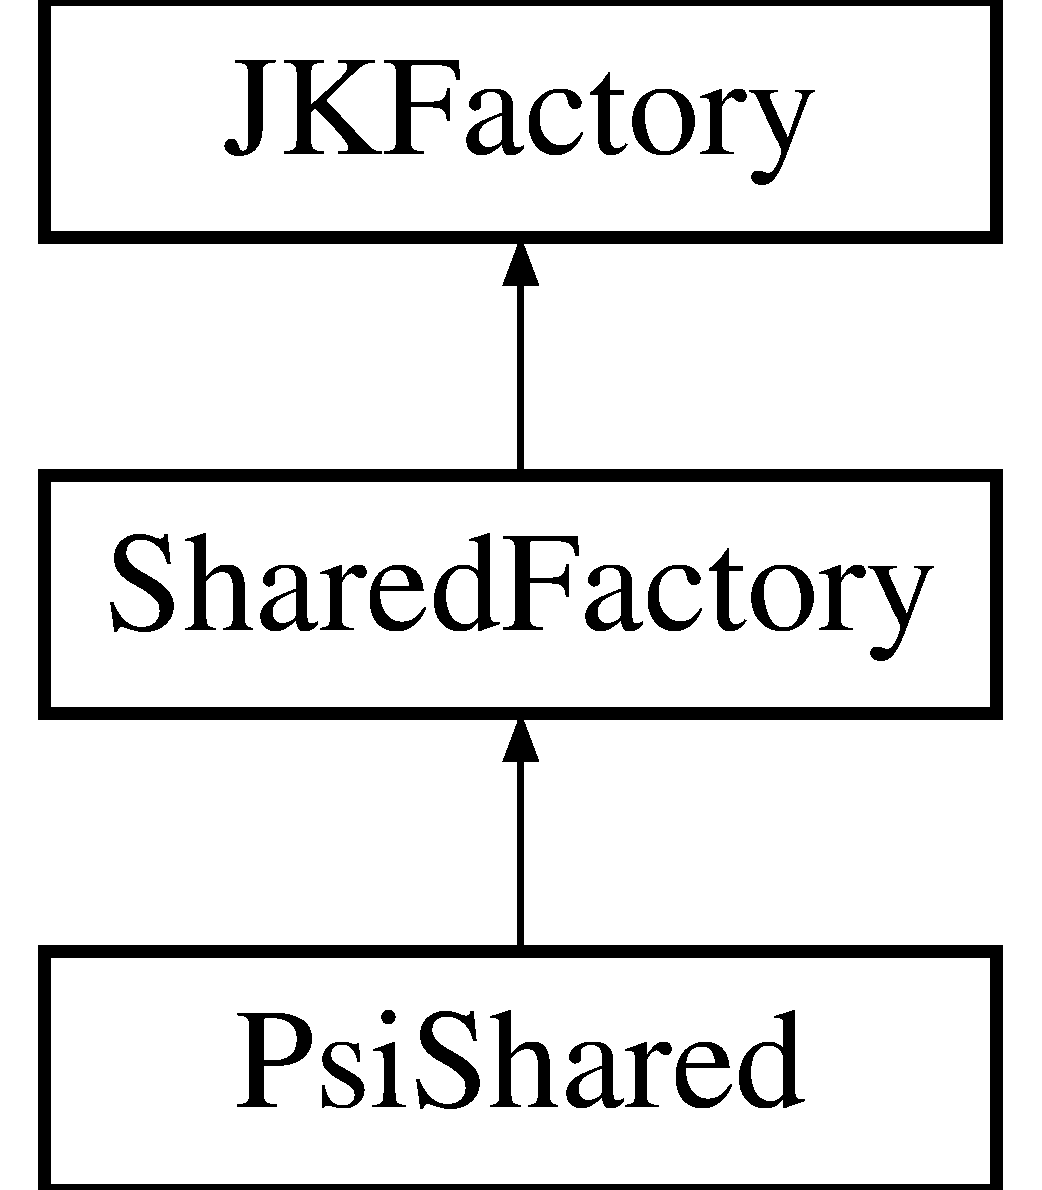
\includegraphics[height=3cm]{classJKBuilder_1_1PsiShared}
\end{center}
\end{figure}
\subsection*{Public Member Functions}
\begin{DoxyCompactItemize}
\item 
void \hyperlink{classJKBuilder_1_1PsiShared_aa5f73a8109ec88464262262164feda1e}{BuildJK} (const double $\ast$DensityMatrix, \hyperlink{namespaceJKBuilder_aef21bc37b7cf7bc5ebb5a48628db8d0f}{SharedSymJKMatrix} \&J\_\-Matrix, \hyperlink{namespaceJKBuilder_aef21bc37b7cf7bc5ebb5a48628db8d0f}{SharedSymJKMatrix} \&K\_\-Matrix)
\begin{DoxyCompactList}\small\item\em The function actually in charge of building the J and K matrices. \item\end{DoxyCompactList}\item 
\hyperlink{classJKBuilder_1_1PsiShared_a6500ac4c346e1a9c8c27f8b9f02bb29b}{PsiShared} (\hyperlink{classJKBuilder_1_1AOBasisSet}{AOBasisSet} $\ast$\hyperlink{classJKBuilder_1_1PsiShared_a33250ff04c740919f41b0ffb6c78ada5}{basis}, \hyperlink{classJKBuilder_1_1Integrals}{Integrals} $\ast$\hyperlink{classJKBuilder_1_1PsiShared_abff505bf91f526e978bc6abbf3e0cfc5}{DaInts})
\end{DoxyCompactItemize}
\subsection*{Protected Attributes}
\begin{DoxyCompactItemize}
\item 
std::vector$<$ \hyperlink{namespaceJKBuilder_a490b0a0cd0b0f8f0e280e29b03eb51a3}{Shared2Matrix} $>$ \hyperlink{classJKBuilder_1_1SharedFactory_afabc3015deddc9247c1c2822431a724f}{J}
\begin{DoxyCompactList}\small\item\em The J \hyperlink{classJKBuilder_1_1matrix}{matrix}. \item\end{DoxyCompactList}\item 
std::vector$<$ \hyperlink{namespaceJKBuilder_a490b0a0cd0b0f8f0e280e29b03eb51a3}{Shared2Matrix} $>$ \hyperlink{classJKBuilder_1_1SharedFactory_a59469c5d5576ee51c033626879e699b1}{K}
\begin{DoxyCompactList}\small\item\em The K \hyperlink{classJKBuilder_1_1matrix}{matrix}. \item\end{DoxyCompactList}\item 
std::vector$<$ \hyperlink{namespaceJKBuilder_a490b0a0cd0b0f8f0e280e29b03eb51a3}{Shared2Matrix} $>$ \hyperlink{classJKBuilder_1_1SharedFactory_af21e4022fc5e357635e5b22bb359fcba}{rho}
\begin{DoxyCompactList}\small\item\em The density. \item\end{DoxyCompactList}\end{DoxyCompactItemize}
\subsection*{Private Member Functions}
\begin{DoxyCompactItemize}
\item 
bool \hyperlink{classJKBuilder_1_1PsiShared_a911b43dc1d1da86bfdbd45e86f4be122}{IsSignificant} (const int i, const int j)
\begin{DoxyCompactList}\small\item\em Replicates Psi's Significance criteria for determining if shell pair i,j should be considered. \item\end{DoxyCompactList}\item 
bool \hyperlink{classJKBuilder_1_1PsiShared_a0ec04bf57470f228eeb9e8f608014edf}{IsSignificant} (const int i, const int j, const int k, const int l)
\begin{DoxyCompactList}\small\item\em The four-\/index version. \item\end{DoxyCompactList}\item 
double \hyperlink{classJKBuilder_1_1PsiShared_af71d3f76014ba72b33336cef6ad2e397}{CalcPrefactor} (const int p, const int q, const int r, const int s)
\begin{DoxyCompactList}\small\item\em Given a shell quartet: pqrs calculates the appropriate weighting factor. \item\end{DoxyCompactList}\item 
void \hyperlink{classJKBuilder_1_1PsiShared_a4b5b1a33d6eb89835454c8b852a1e63b}{FillJK} (std::vector$<$ double $\ast$ $>$ \&JKs, \hyperlink{namespaceJKBuilder_aa50d645c83645be7de5fa94937abf1f3}{SharedBasis} \hyperlink{classJKBuilder_1_1PsiShared_a33250ff04c740919f41b0ffb6c78ada5}{basis}, double $\ast$dp, int $\ast$PQRS, int $\ast$pqrs, const double $\ast$\hyperlink{classJKBuilder_1_1Integrals}{Integrals})
\begin{DoxyCompactList}\small\item\em Given a block of the four electron integrals fills the values into J and K. \item\end{DoxyCompactList}\item 
void \hyperlink{classJKBuilder_1_1PsiShared_ac2d3bee6c0f963913d26d6cc3f7e2403}{FillJK2} (\hyperlink{namespaceJKBuilder_aa50d645c83645be7de5fa94937abf1f3}{SharedBasis} \hyperlink{classJKBuilder_1_1PsiShared_a33250ff04c740919f41b0ffb6c78ada5}{basis}, int P, int Q, double $\ast$JorK, vector$<$ double $\ast$ $>$ JandKs, int index, bool IsSymmetric)
\end{DoxyCompactItemize}
\subsection*{Private Attributes}
\begin{DoxyCompactItemize}
\item 
\hyperlink{namespaceJKBuilder_a5f21cc1a0cc795f1cb9aceca0400dcd0}{SharedInts} \hyperlink{classJKBuilder_1_1PsiShared_abff505bf91f526e978bc6abbf3e0cfc5}{DaInts}
\item 
\hyperlink{namespaceJKBuilder_aa50d645c83645be7de5fa94937abf1f3}{SharedBasis} \hyperlink{classJKBuilder_1_1PsiShared_a33250ff04c740919f41b0ffb6c78ada5}{basis}
\end{DoxyCompactItemize}


\subsection{Constructor \& Destructor Documentation}
\hypertarget{classJKBuilder_1_1PsiShared_a6500ac4c346e1a9c8c27f8b9f02bb29b}{
\index{JKBuilder::PsiShared@{JKBuilder::PsiShared}!PsiShared@{PsiShared}}
\index{PsiShared@{PsiShared}!JKBuilder::PsiShared@{JKBuilder::PsiShared}}
\subsubsection[{PsiShared}]{\setlength{\rightskip}{0pt plus 5cm}{\bf PsiShared} ({\bf AOBasisSet} $\ast$ {\em basis}, \/  {\bf Integrals} $\ast$ {\em DaInts})}}
\label{classJKBuilder_1_1PsiShared_a6500ac4c346e1a9c8c27f8b9f02bb29b}


\subsection{Member Function Documentation}
\hypertarget{classJKBuilder_1_1PsiShared_a911b43dc1d1da86bfdbd45e86f4be122}{
\index{JKBuilder::PsiShared@{JKBuilder::PsiShared}!IsSignificant@{IsSignificant}}
\index{IsSignificant@{IsSignificant}!JKBuilder::PsiShared@{JKBuilder::PsiShared}}
\subsubsection[{IsSignificant}]{\setlength{\rightskip}{0pt plus 5cm}bool IsSignificant (const int {\em i}, \/  const int {\em j})\hspace{0.3cm}{\ttfamily  \mbox{[}private\mbox{]}}}}
\label{classJKBuilder_1_1PsiShared_a911b43dc1d1da86bfdbd45e86f4be122}


Replicates Psi's Significance criteria for determining if shell pair i,j should be considered. Right now this function does nothing because Psi's significance criteria is based on the magnitude of elements of the 4 index electrons, which I don't have a way at yet... \hypertarget{classJKBuilder_1_1PsiShared_a0ec04bf57470f228eeb9e8f608014edf}{
\index{JKBuilder::PsiShared@{JKBuilder::PsiShared}!IsSignificant@{IsSignificant}}
\index{IsSignificant@{IsSignificant}!JKBuilder::PsiShared@{JKBuilder::PsiShared}}
\subsubsection[{IsSignificant}]{\setlength{\rightskip}{0pt plus 5cm}bool IsSignificant (const int {\em i}, \/  const int {\em j}, \/  const int {\em k}, \/  const int {\em l})\hspace{0.3cm}{\ttfamily  \mbox{[}private\mbox{]}}}}
\label{classJKBuilder_1_1PsiShared_a0ec04bf57470f228eeb9e8f608014edf}


The four-\/index version. \hypertarget{classJKBuilder_1_1PsiShared_af71d3f76014ba72b33336cef6ad2e397}{
\index{JKBuilder::PsiShared@{JKBuilder::PsiShared}!CalcPrefactor@{CalcPrefactor}}
\index{CalcPrefactor@{CalcPrefactor}!JKBuilder::PsiShared@{JKBuilder::PsiShared}}
\subsubsection[{CalcPrefactor}]{\setlength{\rightskip}{0pt plus 5cm}double CalcPrefactor (const int {\em p}, \/  const int {\em q}, \/  const int {\em r}, \/  const int {\em s})\hspace{0.3cm}{\ttfamily  \mbox{[}private\mbox{]}}}}
\label{classJKBuilder_1_1PsiShared_af71d3f76014ba72b33336cef6ad2e397}


Given a shell quartet: pqrs calculates the appropriate weighting factor. To understand the origin of this prefactor see the comments regarding FillJK. \hypertarget{classJKBuilder_1_1PsiShared_a4b5b1a33d6eb89835454c8b852a1e63b}{
\index{JKBuilder::PsiShared@{JKBuilder::PsiShared}!FillJK@{FillJK}}
\index{FillJK@{FillJK}!JKBuilder::PsiShared@{JKBuilder::PsiShared}}
\subsubsection[{FillJK}]{\setlength{\rightskip}{0pt plus 5cm}void FillJK (std::vector$<$ double $\ast$ $>$ \& {\em JKs}, \/  {\bf SharedBasis} {\em basis}, \/  double $\ast$ {\em dp}, \/  int $\ast$ {\em PQRS}, \/  int $\ast$ {\em pqrs}, \/  const double $\ast$ {\em Integrals})\hspace{0.3cm}{\ttfamily  \mbox{[}private\mbox{]}}}}
\label{classJKBuilder_1_1PsiShared_a4b5b1a33d6eb89835454c8b852a1e63b}


Given a block of the four electron integrals fills the values into J and K. Assume we have a block of the four electron integrals that corresponds to shells p,q,r, and s on atoms P,Q,R, and S respectively. Letting i,j,k,l be basis functions belonging to shells p,q,r, and s respectively, it is this functions job to fill in J and K respectively.

Elements of J and K are defined in terms of the density \hyperlink{classJKBuilder_1_1matrix}{matrix}, D, and the four electron integrals as: \begin{eqnarray*} J_{ij}=\sum_{kl}D_{kl}(ij|kl)\\ K_{ij}=\sum_{kl}D_{kl}(ik|jl)\\ K_{ik}=\sum_{jl}D_{jl}(ij|kl), \end{eqnarray*} where in the last line we swapped dummy indices for the exchange \hyperlink{classJKBuilder_1_1matrix}{matrix}, so that it is in terms of the same four electron integral element.

Assume that p!=q!=r!=s for the time being, then note that the summation over kl runs over all pairs including lk; however, the iterator will not give us this element because (ij$|$kl)=(ij$|$lk) and we agreed to only iterate over unique elements. This means we have to add both of these at the same time:

\begin{eqnarray*} J_{ij}=\sum_{kl}\left(D_{kl}+D_{lk}\right)(ij|kl)\\ J_{kl}=\sum_{kl}\left(D_{ij}+D_{ji}\right)(ij|kl), \end{eqnarray*}

where the last line accounts for the fact that we agreed not to iterate over (kl$|$ij), which consequently means we are also not iterating over (kl$|$ji), because they all have the same value. Noting the symmetry of the four electron integral, we are also not iterating over (ji$|$kl), (ji$|$lk), (lk$|$ij), and (lk$|$ji), which correspond to elements J\_\-\{ji\} and J\_\-\{lk\} of the Coulomb \hyperlink{classJKBuilder_1_1matrix}{matrix}. Note that : \begin{eqnarray*} J_{ij}=\sum_{kl}\left(D_{kl}+D_{lk}\right)(ij|kl)\\ J_{ji}=\sum_{kl}\left(D_{kl}+D_{lk}\right)(ij|kl)\\ \therefore J_{ij}=J_{ji}\forall\ \{i,j,D\}, \end{eqnarray*} furthermore this is true whether or not D is symmetric (i.e. D\_\-\{kl\}=D\_\-\{lk\}), which means we never have to worry about the last four elements of this list.

What about the exchange \hyperlink{classJKBuilder_1_1matrix}{matrix}? Our discussion of the J \hyperlink{classJKBuilder_1_1matrix}{matrix} shows that for each element (ij$|$kl), we are essentially considering eight elements: (ij$|$kl), (ij$|$lk), (kl$|$ij), (kl$|$ji), (ji$|$kl), (ji$|$lk), (lk$|$ij), and (lk$|$ji). Based on the equation for the exchange \hyperlink{classJKBuilder_1_1matrix}{matrix} given above, this means we need to update elements $K_{ik}$,$K_{il}$,$K_{ki}$, $K_{kj}$, $K_{jk}$, $K_{li}$, and $K_{lj}$ respectively. Unlike the J \hyperlink{classJKBuilder_1_1matrix}{matrix}: \begin{eqnarray*} K_{ik}=\sum_{jl}D_{jl}(ij|kl)\\ K_{ki}=\sum_{lj}D_{lj}(ji|lk)\\ K_{ik}=K_{ki} \iff\ D_{jl}=D_{lj}, \end{eqnarray*} i.e. if D is symmetric, we only need to consider four elements ($K_{ik}$,$K_{il}$,$K_{jk}$ and $K_{jl}$) if it is not we have to consider all 8, bummer....

Now consider what happens if r==s, in that case our assumption that because (ij$|$kl)=(ij$|$lk) we are not going to consider the element (ij$|$lk) are false (because we iterate each index over the entire range). And if we use the same code, we will double count this integral. Of course an analogous situation exists for p==q and when both are true we actually quadruple count. Less obvious is that when p==r and q==s, also leads to a double counting (not quadruple) scenario; this case stems from assuming we are only going to consider (ij$|$kl) and not (kl$|$ij). Note that p==r or q==s alone corresponds to considering (ij$|$kl) and (kj$|$il) \mbox{[}or (il$|$kj) for the q==s case\mbox{]}, which need to be considered, i.e. there is no general symmetry relation between them. It follows that for the case when p==q==r==s we octuple count the quantity. This is what the prefactor function above accounts for.

It seems to me that these \char`\"{}fringe\char`\"{} cases are actually quite common... TODO: Check if we get a much faster code by omitting these \char`\"{}fringe\char`\"{} cases from the summations. \hypertarget{classJKBuilder_1_1PsiShared_ac2d3bee6c0f963913d26d6cc3f7e2403}{
\index{JKBuilder::PsiShared@{JKBuilder::PsiShared}!FillJK2@{FillJK2}}
\index{FillJK2@{FillJK2}!JKBuilder::PsiShared@{JKBuilder::PsiShared}}
\subsubsection[{FillJK2}]{\setlength{\rightskip}{0pt plus 5cm}void FillJK2 ({\bf SharedBasis} {\em basis}, \/  int {\em P}, \/  int {\em Q}, \/  double $\ast$ {\em JorK}, \/  vector$<$ double $\ast$ $>$ {\em JandKs}, \/  int {\em index}, \/  bool {\em IsSymmetric})\hspace{0.3cm}{\ttfamily  \mbox{[}private\mbox{]}}}}
\label{classJKBuilder_1_1PsiShared_ac2d3bee6c0f963913d26d6cc3f7e2403}
\hypertarget{classJKBuilder_1_1PsiShared_aa5f73a8109ec88464262262164feda1e}{
\index{JKBuilder::PsiShared@{JKBuilder::PsiShared}!BuildJK@{BuildJK}}
\index{BuildJK@{BuildJK}!JKBuilder::PsiShared@{JKBuilder::PsiShared}}
\subsubsection[{BuildJK}]{\setlength{\rightskip}{0pt plus 5cm}void BuildJK (const double $\ast$ {\em DensityMatrix}, \/  {\bf SharedSymJKMatrix} \& {\em J\_\-Matrix}, \/  {\bf SharedSymJKMatrix} \& {\em K\_\-Matrix})\hspace{0.3cm}{\ttfamily  \mbox{[}virtual\mbox{]}}}}
\label{classJKBuilder_1_1PsiShared_aa5f73a8109ec88464262262164feda1e}


The function actually in charge of building the J and K matrices. This function first updates the density \hyperlink{classJKBuilder_1_1matrix}{matrix} to be the one given to it. Next, it computes J and K and returns them as \hyperlink{classJKBuilder_1_1matrix}{matrix} objects.


\begin{DoxyParams}{Parameters}
\item[\mbox{$\leftarrow$} {\em DensityMatrix}]The density \hyperlink{classJKBuilder_1_1matrix}{matrix} \item[\mbox{$\rightarrow$} {\em J}]The Coulomb \hyperlink{classJKBuilder_1_1matrix}{matrix} corresponding to DensityMatrix \item[\mbox{$\rightarrow$} {\em K}]The Exchange \hyperlink{classJKBuilder_1_1matrix}{matrix} corresponding to DensityMatrix \end{DoxyParams}


Implements \hyperlink{classJKBuilder_1_1JKFactory_ae253b309dafe3ce003fdabfd315318b8}{JKFactory}.

\subsection{Member Data Documentation}
\hypertarget{classJKBuilder_1_1PsiShared_abff505bf91f526e978bc6abbf3e0cfc5}{
\index{JKBuilder::PsiShared@{JKBuilder::PsiShared}!DaInts@{DaInts}}
\index{DaInts@{DaInts}!JKBuilder::PsiShared@{JKBuilder::PsiShared}}
\subsubsection[{DaInts}]{\setlength{\rightskip}{0pt plus 5cm}{\bf SharedInts} {\bf DaInts}\hspace{0.3cm}{\ttfamily  \mbox{[}private\mbox{]}}}}
\label{classJKBuilder_1_1PsiShared_abff505bf91f526e978bc6abbf3e0cfc5}
\hypertarget{classJKBuilder_1_1PsiShared_a33250ff04c740919f41b0ffb6c78ada5}{
\index{JKBuilder::PsiShared@{JKBuilder::PsiShared}!basis@{basis}}
\index{basis@{basis}!JKBuilder::PsiShared@{JKBuilder::PsiShared}}
\subsubsection[{basis}]{\setlength{\rightskip}{0pt plus 5cm}{\bf SharedBasis} {\bf basis}\hspace{0.3cm}{\ttfamily  \mbox{[}private\mbox{]}}}}
\label{classJKBuilder_1_1PsiShared_a33250ff04c740919f41b0ffb6c78ada5}
\hypertarget{classJKBuilder_1_1SharedFactory_afabc3015deddc9247c1c2822431a724f}{
\index{JKBuilder::PsiShared@{JKBuilder::PsiShared}!J@{J}}
\index{J@{J}!JKBuilder::PsiShared@{JKBuilder::PsiShared}}
\subsubsection[{J}]{\setlength{\rightskip}{0pt plus 5cm}std::vector$<${\bf Shared2Matrix}$>$ {\bf J}\hspace{0.3cm}{\ttfamily  \mbox{[}protected, inherited\mbox{]}}}}
\label{classJKBuilder_1_1SharedFactory_afabc3015deddc9247c1c2822431a724f}


The J \hyperlink{classJKBuilder_1_1matrix}{matrix}. \hypertarget{classJKBuilder_1_1SharedFactory_a59469c5d5576ee51c033626879e699b1}{
\index{JKBuilder::PsiShared@{JKBuilder::PsiShared}!K@{K}}
\index{K@{K}!JKBuilder::PsiShared@{JKBuilder::PsiShared}}
\subsubsection[{K}]{\setlength{\rightskip}{0pt plus 5cm}std::vector$<${\bf Shared2Matrix}$>$ {\bf K}\hspace{0.3cm}{\ttfamily  \mbox{[}protected, inherited\mbox{]}}}}
\label{classJKBuilder_1_1SharedFactory_a59469c5d5576ee51c033626879e699b1}


The K \hyperlink{classJKBuilder_1_1matrix}{matrix}. \hypertarget{classJKBuilder_1_1SharedFactory_af21e4022fc5e357635e5b22bb359fcba}{
\index{JKBuilder::PsiShared@{JKBuilder::PsiShared}!rho@{rho}}
\index{rho@{rho}!JKBuilder::PsiShared@{JKBuilder::PsiShared}}
\subsubsection[{rho}]{\setlength{\rightskip}{0pt plus 5cm}std::vector$<${\bf Shared2Matrix}$>$ {\bf rho}\hspace{0.3cm}{\ttfamily  \mbox{[}protected, inherited\mbox{]}}}}
\label{classJKBuilder_1_1SharedFactory_af21e4022fc5e357635e5b22bb359fcba}


The density. 

The documentation for this class was generated from the following files:\begin{DoxyCompactItemize}
\item 
src/\hyperlink{PsiShared_8h}{PsiShared.h}\item 
src/\hyperlink{PsiShared_8cpp}{PsiShared.cpp}\end{DoxyCompactItemize}

\hypertarget{classJKBuilder_1_1QuartetIterator}{
\section{QuartetIterator Class Reference}
\label{classJKBuilder_1_1QuartetIterator}\index{JKBuilder::QuartetIterator@{JKBuilder::QuartetIterator}}
}


Generalization to an iterator that iterates over two pairs of pairs.  


{\ttfamily \#include $<$Iterators.h$>$}Inheritance diagram for QuartetIterator::\begin{figure}[H]
\begin{center}
\leavevmode
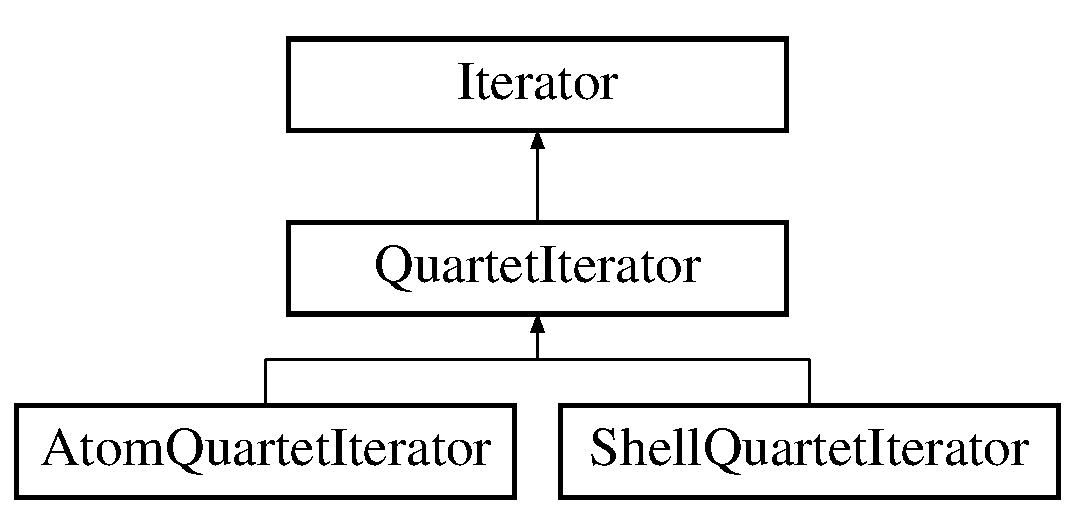
\includegraphics[height=3cm]{classJKBuilder_1_1QuartetIterator}
\end{center}
\end{figure}
\subsection*{Public Member Functions}
\begin{DoxyCompactItemize}
\item 
void \hyperlink{classJKBuilder_1_1QuartetIterator_a34ca36a99b20ae3170babadaffe51ed2}{Start} (int n=0)
\begin{DoxyCompactList}\small\item\em Returns an iterator suitable for starting on iteration n. \item\end{DoxyCompactList}\item 
void \hyperlink{classJKBuilder_1_1QuartetIterator_a5f692b73d2e160450f4617bb75825e11}{End} (int n=-\/1)
\begin{DoxyCompactList}\small\item\em Returns an iterator representing the state of the iterator after n iterations have occured. \item\end{DoxyCompactList}\item 
\hyperlink{classJKBuilder_1_1QuartetIterator_a07d00ea07b0f26457f2552be518080ba}{QuartetIterator} ()
\item 
\hyperlink{classJKBuilder_1_1QuartetIterator_af4c9d6672dc0009768dd792e7f98ae7d}{QuartetIterator} (\hyperlink{classJKBuilder_1_1QuartetIterator}{QuartetIterator} const \&other)
\item 
virtual \hyperlink{classJKBuilder_1_1QuartetIterator_a45af941f47c9b8051f2ed69d47157e12}{$\sim$QuartetIterator} ()
\item 
\hyperlink{classJKBuilder_1_1QuartetIterator}{QuartetIterator} \& \hyperlink{classJKBuilder_1_1QuartetIterator_ab3cd17222545586596dbbc6aa3ca7046}{operator=} (\hyperlink{classJKBuilder_1_1QuartetIterator}{QuartetIterator} const \&other)
\item 
\hyperlink{classJKBuilder_1_1Iterator}{Iterator} \hyperlink{classJKBuilder_1_1Iterator_ac1702aedba13b4112b891b58dfd78eba}{operator++} (int)
\begin{DoxyCompactList}\small\item\em Increments the iterator after returning it's value. \item\end{DoxyCompactList}\item 
\hyperlink{classJKBuilder_1_1Iterator}{Iterator} \& \hyperlink{classJKBuilder_1_1Iterator_ae1f21c74128a5ef5d1b9de72ceb09be8}{operator++} ()
\begin{DoxyCompactList}\small\item\em Increments the iterator before returning it's value. \item\end{DoxyCompactList}\item 
bool \hyperlink{classJKBuilder_1_1Iterator_a1ea001976a5bc8ae8dc365e2a912b59a}{operator==} (const \hyperlink{classJKBuilder_1_1Iterator}{Iterator} \&other) const 
\item 
bool \hyperlink{classJKBuilder_1_1Iterator_a8c06af8ae0d9d1614ae9f81629275926}{operator!=} (const \hyperlink{classJKBuilder_1_1Iterator}{Iterator} \&other)
\begin{DoxyCompactList}\small\item\em Returns the opposite of operator==. \item\end{DoxyCompactList}\item 
void \hyperlink{classJKBuilder_1_1Iterator_aa83de505e29125c1d3ac7bb1b13ca15a}{SetStart} (std::vector$<$ int $>$ const \&other)
\begin{DoxyCompactList}\small\item\em Sets the N Indices to the N given in other. \item\end{DoxyCompactList}\item 
void \hyperlink{classJKBuilder_1_1Iterator_aad84ec668b5f41210db34c540aaa31fc}{SetEnd} (std::vector$<$ int $>$ const \&other)
\begin{DoxyCompactList}\small\item\em Sets the N MaxInd in other. \item\end{DoxyCompactList}\item 
int \hyperlink{classJKBuilder_1_1Iterator_a74247cf730a06b23fcb1ec64e5596b25}{operator\mbox{[}$\,$\mbox{]}} (const int i) const 
\begin{DoxyCompactList}\small\item\em Returns index i. \item\end{DoxyCompactList}\end{DoxyCompactItemize}
\subsection*{Protected Member Functions}
\begin{DoxyCompactItemize}
\item 
virtual bool \hyperlink{classJKBuilder_1_1QuartetIterator_af88c46759ac710bbd36c17601dc62d55}{RSIsMaxed} ()=0
\begin{DoxyCompactList}\small\item\em The definition of what it means for RS to be maxed. \item\end{DoxyCompactList}\item 
virtual bool \hyperlink{classJKBuilder_1_1QuartetIterator_ac51ff9a02f4a201598f7820476c52faf}{RSIsOK} ()=0
\begin{DoxyCompactList}\small\item\em A check to see if the iterated RS value is acceptable. \item\end{DoxyCompactList}\item 
virtual void \hyperlink{classJKBuilder_1_1QuartetIterator_a7874a07e98b52f4f147cde6f39353bae}{Iterate} ()
\item 
void \hyperlink{classJKBuilder_1_1QuartetIterator_a1af5c865d6e9cfe63d0dedc53bdc13ba}{UpdateCurrentValue} ()
\begin{DoxyCompactList}\small\item\em Copies PQ and RS into CurrentValue. \item\end{DoxyCompactList}\end{DoxyCompactItemize}
\subsection*{Protected Attributes}
\begin{DoxyCompactItemize}
\item 
\hyperlink{classJKBuilder_1_1PairIterator}{PairIterator} $\ast$ \hyperlink{classJKBuilder_1_1QuartetIterator_a84f5c3632fba19d3bb85e1cffb9e51f7}{PQ}
\item 
\hyperlink{classJKBuilder_1_1PairIterator}{PairIterator} $\ast$ \hyperlink{classJKBuilder_1_1QuartetIterator_a26b777bf7ea22524f1cc725020ee2082}{RS}
\item 
std::vector$<$ int $>$ \hyperlink{classJKBuilder_1_1Iterator_a20ca24f6d827aba144bb087c4bcb74a0}{CurrentValue}
\begin{DoxyCompactList}\small\item\em The current value. \item\end{DoxyCompactList}\item 
std::vector$<$ int $>$ \hyperlink{classJKBuilder_1_1Iterator_ab6b56d3c4e9353bc938dd6249cde9ca0}{MaxInd}
\begin{DoxyCompactList}\small\item\em This is a vector of length N containing the maximum each index can be. \item\end{DoxyCompactList}\end{DoxyCompactItemize}
\subsection*{Private Member Functions}
\begin{DoxyCompactItemize}
\item 
void \hyperlink{classJKBuilder_1_1QuartetIterator_a1cc9d53b063e002ead95abb45f05f0c3}{Copy} (\hyperlink{classJKBuilder_1_1QuartetIterator}{QuartetIterator} const \&other)
\end{DoxyCompactItemize}


\subsection{Detailed Description}
Generalization to an iterator that iterates over two pairs of pairs. 

\subsection{Constructor \& Destructor Documentation}
\hypertarget{classJKBuilder_1_1QuartetIterator_a07d00ea07b0f26457f2552be518080ba}{
\index{JKBuilder::QuartetIterator@{JKBuilder::QuartetIterator}!QuartetIterator@{QuartetIterator}}
\index{QuartetIterator@{QuartetIterator}!JKBuilder::QuartetIterator@{JKBuilder::QuartetIterator}}
\subsubsection[{QuartetIterator}]{\setlength{\rightskip}{0pt plus 5cm}{\bf QuartetIterator} ()}}
\label{classJKBuilder_1_1QuartetIterator_a07d00ea07b0f26457f2552be518080ba}
\hypertarget{classJKBuilder_1_1QuartetIterator_af4c9d6672dc0009768dd792e7f98ae7d}{
\index{JKBuilder::QuartetIterator@{JKBuilder::QuartetIterator}!QuartetIterator@{QuartetIterator}}
\index{QuartetIterator@{QuartetIterator}!JKBuilder::QuartetIterator@{JKBuilder::QuartetIterator}}
\subsubsection[{QuartetIterator}]{\setlength{\rightskip}{0pt plus 5cm}{\bf QuartetIterator} ({\bf QuartetIterator} const \& {\em other})}}
\label{classJKBuilder_1_1QuartetIterator_af4c9d6672dc0009768dd792e7f98ae7d}
\hypertarget{classJKBuilder_1_1QuartetIterator_a45af941f47c9b8051f2ed69d47157e12}{
\index{JKBuilder::QuartetIterator@{JKBuilder::QuartetIterator}!$\sim$QuartetIterator@{$\sim$QuartetIterator}}
\index{$\sim$QuartetIterator@{$\sim$QuartetIterator}!JKBuilder::QuartetIterator@{JKBuilder::QuartetIterator}}
\subsubsection[{$\sim$QuartetIterator}]{\setlength{\rightskip}{0pt plus 5cm}$\sim${\bf QuartetIterator} ()\hspace{0.3cm}{\ttfamily  \mbox{[}virtual\mbox{]}}}}
\label{classJKBuilder_1_1QuartetIterator_a45af941f47c9b8051f2ed69d47157e12}


\subsection{Member Function Documentation}
\hypertarget{classJKBuilder_1_1QuartetIterator_a1cc9d53b063e002ead95abb45f05f0c3}{
\index{JKBuilder::QuartetIterator@{JKBuilder::QuartetIterator}!Copy@{Copy}}
\index{Copy@{Copy}!JKBuilder::QuartetIterator@{JKBuilder::QuartetIterator}}
\subsubsection[{Copy}]{\setlength{\rightskip}{0pt plus 5cm}void Copy ({\bf QuartetIterator} const \& {\em other})\hspace{0.3cm}{\ttfamily  \mbox{[}private\mbox{]}}}}
\label{classJKBuilder_1_1QuartetIterator_a1cc9d53b063e002ead95abb45f05f0c3}


Reimplemented from \hyperlink{classJKBuilder_1_1Iterator_aacb7559eb1b8aab6e7bb6a56602d97ff}{Iterator}.\hypertarget{classJKBuilder_1_1QuartetIterator_af88c46759ac710bbd36c17601dc62d55}{
\index{JKBuilder::QuartetIterator@{JKBuilder::QuartetIterator}!RSIsMaxed@{RSIsMaxed}}
\index{RSIsMaxed@{RSIsMaxed}!JKBuilder::QuartetIterator@{JKBuilder::QuartetIterator}}
\subsubsection[{RSIsMaxed}]{\setlength{\rightskip}{0pt plus 5cm}virtual bool RSIsMaxed ()\hspace{0.3cm}{\ttfamily  \mbox{[}protected, pure virtual\mbox{]}}}}
\label{classJKBuilder_1_1QuartetIterator_af88c46759ac710bbd36c17601dc62d55}


The definition of what it means for RS to be maxed. 

Implemented in \hyperlink{classJKBuilder_1_1AtomQuartetIterator_a458dcf49c4c4bbb1e3d3d39d3dc086c9}{AtomQuartetIterator}, and \hyperlink{classJKBuilder_1_1ShellQuartetIterator_a458dcf49c4c4bbb1e3d3d39d3dc086c9}{ShellQuartetIterator}.\hypertarget{classJKBuilder_1_1QuartetIterator_ac51ff9a02f4a201598f7820476c52faf}{
\index{JKBuilder::QuartetIterator@{JKBuilder::QuartetIterator}!RSIsOK@{RSIsOK}}
\index{RSIsOK@{RSIsOK}!JKBuilder::QuartetIterator@{JKBuilder::QuartetIterator}}
\subsubsection[{RSIsOK}]{\setlength{\rightskip}{0pt plus 5cm}virtual bool RSIsOK ()\hspace{0.3cm}{\ttfamily  \mbox{[}protected, pure virtual\mbox{]}}}}
\label{classJKBuilder_1_1QuartetIterator_ac51ff9a02f4a201598f7820476c52faf}


A check to see if the iterated RS value is acceptable. 

Implemented in \hyperlink{classJKBuilder_1_1AtomQuartetIterator_a13e657ea529c0566a0bf48e9c5a488d7}{AtomQuartetIterator}, and \hyperlink{classJKBuilder_1_1ShellQuartetIterator_a13e657ea529c0566a0bf48e9c5a488d7}{ShellQuartetIterator}.\hypertarget{classJKBuilder_1_1QuartetIterator_a7874a07e98b52f4f147cde6f39353bae}{
\index{JKBuilder::QuartetIterator@{JKBuilder::QuartetIterator}!Iterate@{Iterate}}
\index{Iterate@{Iterate}!JKBuilder::QuartetIterator@{JKBuilder::QuartetIterator}}
\subsubsection[{Iterate}]{\setlength{\rightskip}{0pt plus 5cm}void Iterate ()\hspace{0.3cm}{\ttfamily  \mbox{[}protected, virtual\mbox{]}}}}
\label{classJKBuilder_1_1QuartetIterator_a7874a07e98b52f4f147cde6f39353bae}


Reimplemented from \hyperlink{classJKBuilder_1_1Iterator_a7874a07e98b52f4f147cde6f39353bae}{Iterator}.\hypertarget{classJKBuilder_1_1QuartetIterator_a1af5c865d6e9cfe63d0dedc53bdc13ba}{
\index{JKBuilder::QuartetIterator@{JKBuilder::QuartetIterator}!UpdateCurrentValue@{UpdateCurrentValue}}
\index{UpdateCurrentValue@{UpdateCurrentValue}!JKBuilder::QuartetIterator@{JKBuilder::QuartetIterator}}
\subsubsection[{UpdateCurrentValue}]{\setlength{\rightskip}{0pt plus 5cm}void UpdateCurrentValue ()\hspace{0.3cm}{\ttfamily  \mbox{[}protected\mbox{]}}}}
\label{classJKBuilder_1_1QuartetIterator_a1af5c865d6e9cfe63d0dedc53bdc13ba}


Copies PQ and RS into CurrentValue. \hypertarget{classJKBuilder_1_1QuartetIterator_a34ca36a99b20ae3170babadaffe51ed2}{
\index{JKBuilder::QuartetIterator@{JKBuilder::QuartetIterator}!Start@{Start}}
\index{Start@{Start}!JKBuilder::QuartetIterator@{JKBuilder::QuartetIterator}}
\subsubsection[{Start}]{\setlength{\rightskip}{0pt plus 5cm}void Start (int {\em n} = {\ttfamily 0})\hspace{0.3cm}{\ttfamily  \mbox{[}virtual\mbox{]}}}}
\label{classJKBuilder_1_1QuartetIterator_a34ca36a99b20ae3170babadaffe51ed2}


Returns an iterator suitable for starting on iteration n. 

Reimplemented from \hyperlink{classJKBuilder_1_1Iterator_a34ca36a99b20ae3170babadaffe51ed2}{Iterator}.\hypertarget{classJKBuilder_1_1QuartetIterator_a5f692b73d2e160450f4617bb75825e11}{
\index{JKBuilder::QuartetIterator@{JKBuilder::QuartetIterator}!End@{End}}
\index{End@{End}!JKBuilder::QuartetIterator@{JKBuilder::QuartetIterator}}
\subsubsection[{End}]{\setlength{\rightskip}{0pt plus 5cm}void End (int {\em n} = {\ttfamily -\/1})\hspace{0.3cm}{\ttfamily  \mbox{[}virtual\mbox{]}}}}
\label{classJKBuilder_1_1QuartetIterator_a5f692b73d2e160450f4617bb75825e11}


Returns an iterator representing the state of the iterator after n iterations have occured. The default argument is n=-\/1, which is a flag corresponding to the last iteration of the iterator 

Reimplemented from \hyperlink{classJKBuilder_1_1Iterator_a5f692b73d2e160450f4617bb75825e11}{Iterator}.\hypertarget{classJKBuilder_1_1QuartetIterator_ab3cd17222545586596dbbc6aa3ca7046}{
\index{JKBuilder::QuartetIterator@{JKBuilder::QuartetIterator}!operator=@{operator=}}
\index{operator=@{operator=}!JKBuilder::QuartetIterator@{JKBuilder::QuartetIterator}}
\subsubsection[{operator=}]{\setlength{\rightskip}{0pt plus 5cm}{\bf QuartetIterator} \& operator= ({\bf QuartetIterator} const \& {\em other})}}
\label{classJKBuilder_1_1QuartetIterator_ab3cd17222545586596dbbc6aa3ca7046}


Reimplemented from \hyperlink{classJKBuilder_1_1Iterator_ae6f4f24e1855d2aaf89a8a60a9f1521b}{Iterator}.

Reimplemented in \hyperlink{classJKBuilder_1_1AtomQuartetIterator_a39f50a07009d2e9e81e1d64da594084f}{AtomQuartetIterator}, and \hyperlink{classJKBuilder_1_1ShellQuartetIterator_acd8ac6ed2e831bcb87e65acc0de747db}{ShellQuartetIterator}.\hypertarget{classJKBuilder_1_1Iterator_ac1702aedba13b4112b891b58dfd78eba}{
\index{JKBuilder::QuartetIterator@{JKBuilder::QuartetIterator}!operator++@{operator++}}
\index{operator++@{operator++}!JKBuilder::QuartetIterator@{JKBuilder::QuartetIterator}}
\subsubsection[{operator++}]{\setlength{\rightskip}{0pt plus 5cm}{\bf Iterator} operator++ (int)\hspace{0.3cm}{\ttfamily  \mbox{[}inherited\mbox{]}}}}
\label{classJKBuilder_1_1Iterator_ac1702aedba13b4112b891b58dfd78eba}


Increments the iterator after returning it's value. \hypertarget{classJKBuilder_1_1Iterator_ae1f21c74128a5ef5d1b9de72ceb09be8}{
\index{JKBuilder::QuartetIterator@{JKBuilder::QuartetIterator}!operator++@{operator++}}
\index{operator++@{operator++}!JKBuilder::QuartetIterator@{JKBuilder::QuartetIterator}}
\subsubsection[{operator++}]{\setlength{\rightskip}{0pt plus 5cm}{\bf Iterator} \& operator++ ()\hspace{0.3cm}{\ttfamily  \mbox{[}inherited\mbox{]}}}}
\label{classJKBuilder_1_1Iterator_ae1f21c74128a5ef5d1b9de72ceb09be8}


Increments the iterator before returning it's value. \hypertarget{classJKBuilder_1_1Iterator_a1ea001976a5bc8ae8dc365e2a912b59a}{
\index{JKBuilder::QuartetIterator@{JKBuilder::QuartetIterator}!operator==@{operator==}}
\index{operator==@{operator==}!JKBuilder::QuartetIterator@{JKBuilder::QuartetIterator}}
\subsubsection[{operator==}]{\setlength{\rightskip}{0pt plus 5cm}bool operator== (const {\bf Iterator} \& {\em other}) const\hspace{0.3cm}{\ttfamily  \mbox{[}inherited\mbox{]}}}}
\label{classJKBuilder_1_1Iterator_a1ea001976a5bc8ae8dc365e2a912b59a}


Reimplemented in \hyperlink{classJKBuilder_1_1PairIterator_a6b4e430066f478e5e400edd39ef93968}{PairIterator}.\hypertarget{classJKBuilder_1_1Iterator_a8c06af8ae0d9d1614ae9f81629275926}{
\index{JKBuilder::QuartetIterator@{JKBuilder::QuartetIterator}!operator!=@{operator!=}}
\index{operator!=@{operator!=}!JKBuilder::QuartetIterator@{JKBuilder::QuartetIterator}}
\subsubsection[{operator!=}]{\setlength{\rightskip}{0pt plus 5cm}bool operator!= (const {\bf Iterator} \& {\em other})\hspace{0.3cm}{\ttfamily  \mbox{[}inherited\mbox{]}}}}
\label{classJKBuilder_1_1Iterator_a8c06af8ae0d9d1614ae9f81629275926}


Returns the opposite of operator==. \hypertarget{classJKBuilder_1_1Iterator_aa83de505e29125c1d3ac7bb1b13ca15a}{
\index{JKBuilder::QuartetIterator@{JKBuilder::QuartetIterator}!SetStart@{SetStart}}
\index{SetStart@{SetStart}!JKBuilder::QuartetIterator@{JKBuilder::QuartetIterator}}
\subsubsection[{SetStart}]{\setlength{\rightskip}{0pt plus 5cm}void SetStart (std::vector$<$ int $>$ const \& {\em other})\hspace{0.3cm}{\ttfamily  \mbox{[}inherited\mbox{]}}}}
\label{classJKBuilder_1_1Iterator_aa83de505e29125c1d3ac7bb1b13ca15a}


Sets the N Indices to the N given in other. \hypertarget{classJKBuilder_1_1Iterator_aad84ec668b5f41210db34c540aaa31fc}{
\index{JKBuilder::QuartetIterator@{JKBuilder::QuartetIterator}!SetEnd@{SetEnd}}
\index{SetEnd@{SetEnd}!JKBuilder::QuartetIterator@{JKBuilder::QuartetIterator}}
\subsubsection[{SetEnd}]{\setlength{\rightskip}{0pt plus 5cm}void SetEnd (std::vector$<$ int $>$ const \& {\em other})\hspace{0.3cm}{\ttfamily  \mbox{[}inherited\mbox{]}}}}
\label{classJKBuilder_1_1Iterator_aad84ec668b5f41210db34c540aaa31fc}


Sets the N MaxInd in other. \hypertarget{classJKBuilder_1_1Iterator_a74247cf730a06b23fcb1ec64e5596b25}{
\index{JKBuilder::QuartetIterator@{JKBuilder::QuartetIterator}!operator\mbox{[}\mbox{]}@{operator[]}}
\index{operator\mbox{[}\mbox{]}@{operator[]}!JKBuilder::QuartetIterator@{JKBuilder::QuartetIterator}}
\subsubsection[{operator[]}]{\setlength{\rightskip}{0pt plus 5cm}int operator\mbox{[}$\,$\mbox{]} (const int {\em i}) const\hspace{0.3cm}{\ttfamily  \mbox{[}inherited\mbox{]}}}}
\label{classJKBuilder_1_1Iterator_a74247cf730a06b23fcb1ec64e5596b25}


Returns index i. 

\subsection{Member Data Documentation}
\hypertarget{classJKBuilder_1_1QuartetIterator_a84f5c3632fba19d3bb85e1cffb9e51f7}{
\index{JKBuilder::QuartetIterator@{JKBuilder::QuartetIterator}!PQ@{PQ}}
\index{PQ@{PQ}!JKBuilder::QuartetIterator@{JKBuilder::QuartetIterator}}
\subsubsection[{PQ}]{\setlength{\rightskip}{0pt plus 5cm}{\bf PairIterator}$\ast$ {\bf PQ}\hspace{0.3cm}{\ttfamily  \mbox{[}protected\mbox{]}}}}
\label{classJKBuilder_1_1QuartetIterator_a84f5c3632fba19d3bb85e1cffb9e51f7}
\hypertarget{classJKBuilder_1_1QuartetIterator_a26b777bf7ea22524f1cc725020ee2082}{
\index{JKBuilder::QuartetIterator@{JKBuilder::QuartetIterator}!RS@{RS}}
\index{RS@{RS}!JKBuilder::QuartetIterator@{JKBuilder::QuartetIterator}}
\subsubsection[{RS}]{\setlength{\rightskip}{0pt plus 5cm}{\bf PairIterator}$\ast$ {\bf RS}\hspace{0.3cm}{\ttfamily  \mbox{[}protected\mbox{]}}}}
\label{classJKBuilder_1_1QuartetIterator_a26b777bf7ea22524f1cc725020ee2082}
\hypertarget{classJKBuilder_1_1Iterator_a20ca24f6d827aba144bb087c4bcb74a0}{
\index{JKBuilder::QuartetIterator@{JKBuilder::QuartetIterator}!CurrentValue@{CurrentValue}}
\index{CurrentValue@{CurrentValue}!JKBuilder::QuartetIterator@{JKBuilder::QuartetIterator}}
\subsubsection[{CurrentValue}]{\setlength{\rightskip}{0pt plus 5cm}std::vector$<$int$>$ {\bf CurrentValue}\hspace{0.3cm}{\ttfamily  \mbox{[}protected, inherited\mbox{]}}}}
\label{classJKBuilder_1_1Iterator_a20ca24f6d827aba144bb087c4bcb74a0}


The current value. \hypertarget{classJKBuilder_1_1Iterator_ab6b56d3c4e9353bc938dd6249cde9ca0}{
\index{JKBuilder::QuartetIterator@{JKBuilder::QuartetIterator}!MaxInd@{MaxInd}}
\index{MaxInd@{MaxInd}!JKBuilder::QuartetIterator@{JKBuilder::QuartetIterator}}
\subsubsection[{MaxInd}]{\setlength{\rightskip}{0pt plus 5cm}std::vector$<$int$>$ {\bf MaxInd}\hspace{0.3cm}{\ttfamily  \mbox{[}protected, inherited\mbox{]}}}}
\label{classJKBuilder_1_1Iterator_ab6b56d3c4e9353bc938dd6249cde9ca0}


This is a vector of length N containing the maximum each index can be. 

The documentation for this class was generated from the following files:\begin{DoxyCompactItemize}
\item 
src/\hyperlink{Iterators_8h}{Iterators.h}\item 
src/\hyperlink{Iterator_8cpp}{Iterator.cpp}\end{DoxyCompactItemize}

\hypertarget{classJKBuilder_1_1SharedFactory}{
\section{SharedFactory Class Reference}
\label{classJKBuilder_1_1SharedFactory}\index{JKBuilder::SharedFactory@{JKBuilder::SharedFactory}}
}


{\ttfamily \#include $<$SharedFactory.h$>$}Inheritance diagram for SharedFactory::\begin{figure}[H]
\begin{center}
\leavevmode
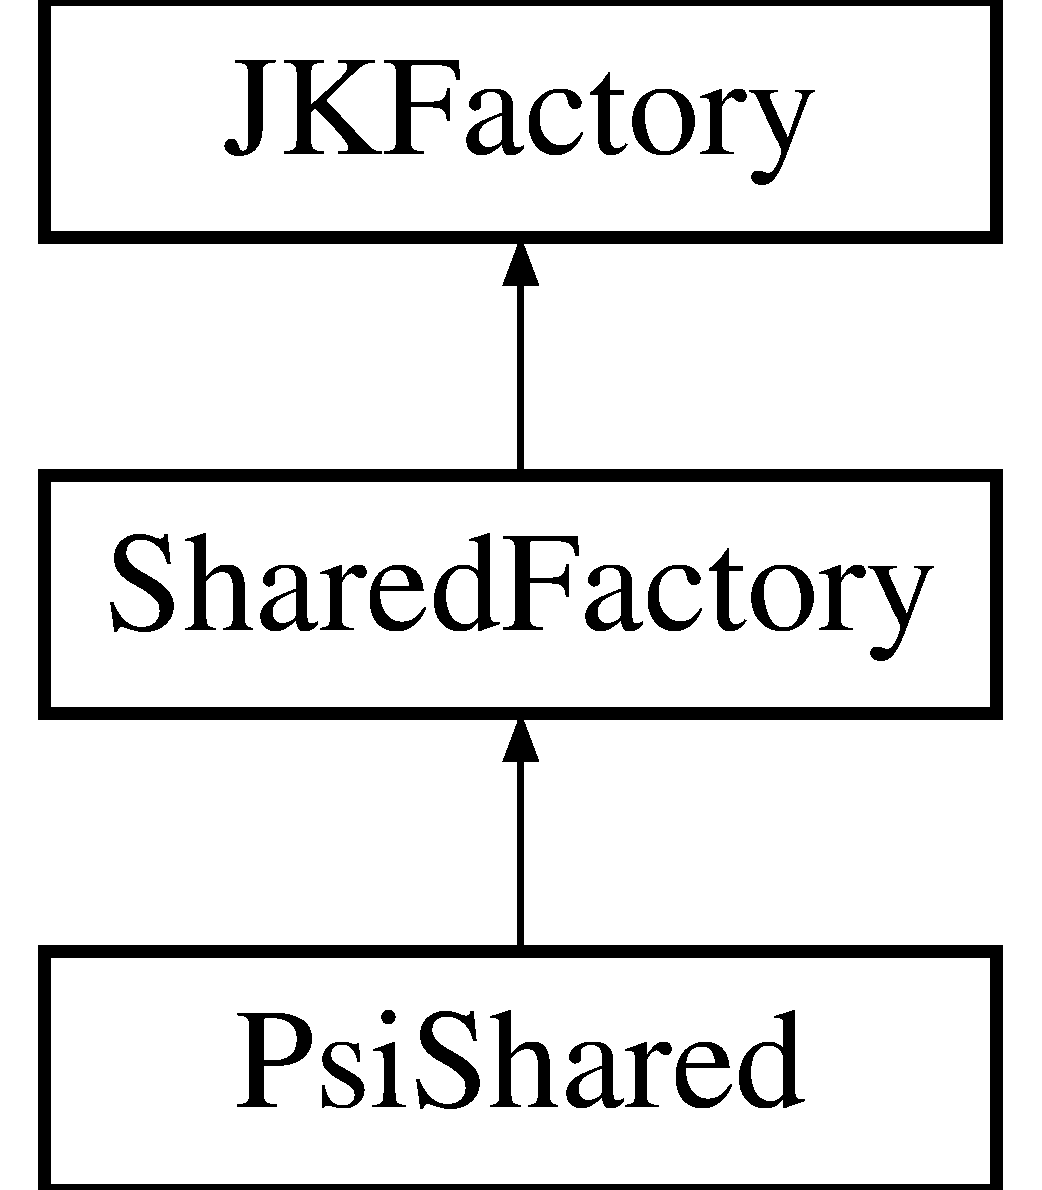
\includegraphics[height=3cm]{classJKBuilder_1_1SharedFactory}
\end{center}
\end{figure}
\subsection*{Public Member Functions}
\begin{DoxyCompactItemize}
\item 
\hyperlink{classJKBuilder_1_1SharedFactory_aaa83ebf150f7d8a94957a024e3b93251}{SharedFactory} (\hyperlink{classJKBuilder_1_1AOBasisSet}{AOBasisSet} $\ast$basis)
\item 
\hyperlink{classJKBuilder_1_1SharedFactory_af0da783c0ceefa7d1f2bf9be1cd53ba6}{$\sim$SharedFactory} ()
\item 
virtual void \hyperlink{classJKBuilder_1_1JKFactory_ae253b309dafe3ce003fdabfd315318b8}{BuildJK} (const double $\ast$DensityMatrix, \hyperlink{namespaceJKBuilder_aef21bc37b7cf7bc5ebb5a48628db8d0f}{SharedSymJKMatrix} \&J\_\-Matrix, \hyperlink{namespaceJKBuilder_aef21bc37b7cf7bc5ebb5a48628db8d0f}{SharedSymJKMatrix} \&K\_\-Matrix)=0
\begin{DoxyCompactList}\small\item\em The function actually in charge of building the J and K matrices. \item\end{DoxyCompactList}\end{DoxyCompactItemize}
\subsection*{Protected Attributes}
\begin{DoxyCompactItemize}
\item 
std::vector$<$ \hyperlink{namespaceJKBuilder_a490b0a0cd0b0f8f0e280e29b03eb51a3}{Shared2Matrix} $>$ \hyperlink{classJKBuilder_1_1SharedFactory_afabc3015deddc9247c1c2822431a724f}{J}
\begin{DoxyCompactList}\small\item\em The J \hyperlink{classJKBuilder_1_1matrix}{matrix}. \item\end{DoxyCompactList}\item 
std::vector$<$ \hyperlink{namespaceJKBuilder_a490b0a0cd0b0f8f0e280e29b03eb51a3}{Shared2Matrix} $>$ \hyperlink{classJKBuilder_1_1SharedFactory_a59469c5d5576ee51c033626879e699b1}{K}
\begin{DoxyCompactList}\small\item\em The K \hyperlink{classJKBuilder_1_1matrix}{matrix}. \item\end{DoxyCompactList}\item 
std::vector$<$ \hyperlink{namespaceJKBuilder_a490b0a0cd0b0f8f0e280e29b03eb51a3}{Shared2Matrix} $>$ \hyperlink{classJKBuilder_1_1SharedFactory_af21e4022fc5e357635e5b22bb359fcba}{rho}
\begin{DoxyCompactList}\small\item\em The density. \item\end{DoxyCompactList}\end{DoxyCompactItemize}


\subsection{Constructor \& Destructor Documentation}
\hypertarget{classJKBuilder_1_1SharedFactory_aaa83ebf150f7d8a94957a024e3b93251}{
\index{JKBuilder::SharedFactory@{JKBuilder::SharedFactory}!SharedFactory@{SharedFactory}}
\index{SharedFactory@{SharedFactory}!JKBuilder::SharedFactory@{JKBuilder::SharedFactory}}
\subsubsection[{SharedFactory}]{\setlength{\rightskip}{0pt plus 5cm}{\bf SharedFactory} ({\bf AOBasisSet} $\ast$ {\em basis})}}
\label{classJKBuilder_1_1SharedFactory_aaa83ebf150f7d8a94957a024e3b93251}
\hypertarget{classJKBuilder_1_1SharedFactory_af0da783c0ceefa7d1f2bf9be1cd53ba6}{
\index{JKBuilder::SharedFactory@{JKBuilder::SharedFactory}!$\sim$SharedFactory@{$\sim$SharedFactory}}
\index{$\sim$SharedFactory@{$\sim$SharedFactory}!JKBuilder::SharedFactory@{JKBuilder::SharedFactory}}
\subsubsection[{$\sim$SharedFactory}]{\setlength{\rightskip}{0pt plus 5cm}$\sim${\bf SharedFactory} ()}}
\label{classJKBuilder_1_1SharedFactory_af0da783c0ceefa7d1f2bf9be1cd53ba6}


\subsection{Member Function Documentation}
\hypertarget{classJKBuilder_1_1JKFactory_ae253b309dafe3ce003fdabfd315318b8}{
\index{JKBuilder::SharedFactory@{JKBuilder::SharedFactory}!BuildJK@{BuildJK}}
\index{BuildJK@{BuildJK}!JKBuilder::SharedFactory@{JKBuilder::SharedFactory}}
\subsubsection[{BuildJK}]{\setlength{\rightskip}{0pt plus 5cm}virtual void BuildJK (const double $\ast$ {\em DensityMatrix}, \/  {\bf SharedSymJKMatrix} \& {\em J\_\-Matrix}, \/  {\bf SharedSymJKMatrix} \& {\em K\_\-Matrix})\hspace{0.3cm}{\ttfamily  \mbox{[}pure virtual, inherited\mbox{]}}}}
\label{classJKBuilder_1_1JKFactory_ae253b309dafe3ce003fdabfd315318b8}


The function actually in charge of building the J and K matrices. This function first updates the density \hyperlink{classJKBuilder_1_1matrix}{matrix} to be the one given to it. Next, it computes J and K and returns them as \hyperlink{classJKBuilder_1_1matrix}{matrix} objects.


\begin{DoxyParams}{Parameters}
\item[\mbox{$\leftarrow$} {\em DensityMatrix}]The density \hyperlink{classJKBuilder_1_1matrix}{matrix} \item[\mbox{$\rightarrow$} {\em J}]The Coulomb \hyperlink{classJKBuilder_1_1matrix}{matrix} corresponding to DensityMatrix \item[\mbox{$\rightarrow$} {\em K}]The Exchange \hyperlink{classJKBuilder_1_1matrix}{matrix} corresponding to DensityMatrix \end{DoxyParams}


Implemented in \hyperlink{classGTFock_1_1DistGTFock_aea85d0b3d84e8e52819e8a15201e078a}{DistGTFock}, and \hyperlink{classJKBuilder_1_1PsiShared_aa5f73a8109ec88464262262164feda1e}{PsiShared}.

\subsection{Member Data Documentation}
\hypertarget{classJKBuilder_1_1SharedFactory_afabc3015deddc9247c1c2822431a724f}{
\index{JKBuilder::SharedFactory@{JKBuilder::SharedFactory}!J@{J}}
\index{J@{J}!JKBuilder::SharedFactory@{JKBuilder::SharedFactory}}
\subsubsection[{J}]{\setlength{\rightskip}{0pt plus 5cm}std::vector$<${\bf Shared2Matrix}$>$ {\bf J}\hspace{0.3cm}{\ttfamily  \mbox{[}protected\mbox{]}}}}
\label{classJKBuilder_1_1SharedFactory_afabc3015deddc9247c1c2822431a724f}


The J \hyperlink{classJKBuilder_1_1matrix}{matrix}. \hypertarget{classJKBuilder_1_1SharedFactory_a59469c5d5576ee51c033626879e699b1}{
\index{JKBuilder::SharedFactory@{JKBuilder::SharedFactory}!K@{K}}
\index{K@{K}!JKBuilder::SharedFactory@{JKBuilder::SharedFactory}}
\subsubsection[{K}]{\setlength{\rightskip}{0pt plus 5cm}std::vector$<${\bf Shared2Matrix}$>$ {\bf K}\hspace{0.3cm}{\ttfamily  \mbox{[}protected\mbox{]}}}}
\label{classJKBuilder_1_1SharedFactory_a59469c5d5576ee51c033626879e699b1}


The K \hyperlink{classJKBuilder_1_1matrix}{matrix}. \hypertarget{classJKBuilder_1_1SharedFactory_af21e4022fc5e357635e5b22bb359fcba}{
\index{JKBuilder::SharedFactory@{JKBuilder::SharedFactory}!rho@{rho}}
\index{rho@{rho}!JKBuilder::SharedFactory@{JKBuilder::SharedFactory}}
\subsubsection[{rho}]{\setlength{\rightskip}{0pt plus 5cm}std::vector$<${\bf Shared2Matrix}$>$ {\bf rho}\hspace{0.3cm}{\ttfamily  \mbox{[}protected\mbox{]}}}}
\label{classJKBuilder_1_1SharedFactory_af21e4022fc5e357635e5b22bb359fcba}


The density. 

The documentation for this class was generated from the following files:\begin{DoxyCompactItemize}
\item 
src/\hyperlink{SharedFactory_8h}{SharedFactory.h}\item 
src/\hyperlink{SharedFactory_8cpp}{SharedFactory.cpp}\end{DoxyCompactItemize}

\hypertarget{classJKBuilder_1_1SharedMatrix}{
\section{SharedMatrix Class Reference}
\label{classJKBuilder_1_1SharedMatrix}\index{JKBuilder::SharedMatrix@{JKBuilder::SharedMatrix}}
}


{\ttfamily \#include $<$SharedMatrix.h$>$}Inheritance diagram for SharedMatrix::\begin{figure}[H]
\begin{center}
\leavevmode
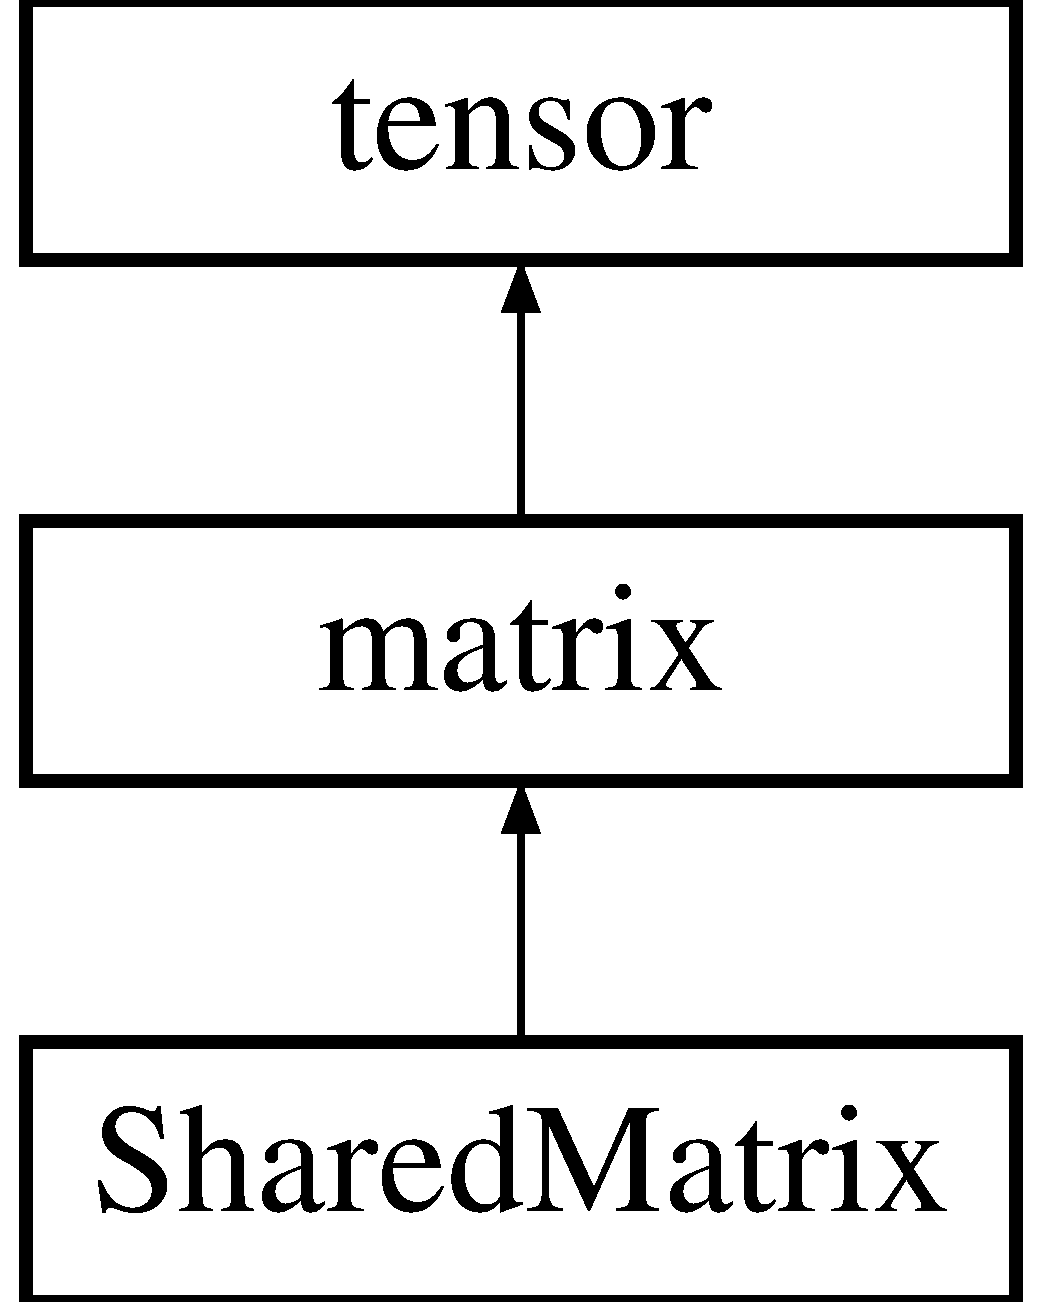
\includegraphics[height=3cm]{classJKBuilder_1_1SharedMatrix}
\end{center}
\end{figure}
\subsection*{Public Member Functions}
\begin{DoxyCompactItemize}
\item 
\hyperlink{classJKBuilder_1_1SharedMatrix_af772312dbed003a511b08981c4867a86}{SharedMatrix} (const int n, const int m, const bool init=false)
\item 
void \hyperlink{classJKBuilder_1_1matrix_af2563817f6505e9f8a6ee5c5c209a115}{T} ()
\begin{DoxyCompactList}\small\item\em Transposes a \hyperlink{classJKBuilder_1_1matrix}{matrix} by flipping the flag (don't forget to un-\/transpose it). \item\end{DoxyCompactList}\item 
const double \& \hyperlink{classJKBuilder_1_1matrix_a9ccbac42f4eefb704f04886001f4fb3e}{operator()} (const int i, const int j) const 
\begin{DoxyCompactList}\small\item\em Returns a non-\/editable element (i,j). \item\end{DoxyCompactList}\item 
double \& \hyperlink{classJKBuilder_1_1matrix_a3d7fca183ff1c9f4c160218746f2ef31}{operator()} (const int i, const int j)
\begin{DoxyCompactList}\small\item\em Returns an editable element (i,j). \item\end{DoxyCompactList}\item 
\hyperlink{classJKBuilder_1_1matrix}{matrix} \& \hyperlink{classJKBuilder_1_1matrix_ad4799cbe4a5d07c77f41857a3ce914a2}{operator$\ast$} (const double alpha)
\begin{DoxyCompactList}\small\item\em Scales a \hyperlink{classJKBuilder_1_1matrix}{matrix} by alpha. \item\end{DoxyCompactList}\item 
void \hyperlink{classJKBuilder_1_1tensor_a0ca5cbe96d2a61f06ae4b543ef84f166}{Alloc} ()
\item 
bool \hyperlink{classJKBuilder_1_1tensor_a79c9a36acc5dbeab94033ca97971dc09}{IsSet} () const 
\begin{DoxyCompactList}\small\item\em Returns true if this \hyperlink{classJKBuilder_1_1tensor}{tensor} is allocated and DimsGood==true (roughly the equiv to asking if this is NULL). \item\end{DoxyCompactList}\item 
virtual void \hyperlink{classJKBuilder_1_1tensor_a98b1050f09da390896f964fb7a892391}{Initialize} ()
\begin{DoxyCompactList}\small\item\em Sets all elements to zero in the \hyperlink{classJKBuilder_1_1tensor}{tensor}, which obviously overwrites the contents. \item\end{DoxyCompactList}\item 
virtual void \hyperlink{classJKBuilder_1_1tensor_a10ffea2bf428adfa3e8319646c44a3c6}{Update} (const double $\ast$Tensor)
\begin{DoxyCompactList}\small\item\em Updates DaTensor so that it is the same as Tensor. \item\end{DoxyCompactList}\item 
int \hyperlink{classJKBuilder_1_1tensor_a537b2f14296e2f0e62f00e1703c5fa08}{TotalElements} ()
\item 
int \hyperlink{classJKBuilder_1_1tensor_a6bdcfca6493bc217b607317dbceb28b2}{DimI} (const int i) const 
\begin{DoxyCompactList}\small\item\em Returns dimension i (counting from 0). \item\end{DoxyCompactList}\item 
void \hyperlink{classJKBuilder_1_1tensor_ace6bcf62c74395ab9e37abc4935f66e0}{SetDimensions} (const int $\ast$DesiredDimensions)
\begin{DoxyCompactList}\small\item\em Copies the dimensions you want (DesiredDimensions), into the \hyperlink{classJKBuilder_1_1tensor_a2ce1e6e0782ddee097f2c4aa2663d3e9}{tensor::dimensions}. Overwrites the contents. \item\end{DoxyCompactList}\item 
virtual void \hyperlink{classJKBuilder_1_1tensor_a388f572c62279f839ee138a9afbdeeb5}{print} ()
\begin{DoxyCompactList}\small\item\em Debugging function that prints the \hyperlink{classJKBuilder_1_1tensor}{tensor} (current model not appropriate for a distributed \hyperlink{classJKBuilder_1_1tensor}{tensor}) to the \hyperlink{classJKBuilder_1_1printer}{printer}. \item\end{DoxyCompactList}\item 
virtual void \hyperlink{classJKBuilder_1_1tensor_a74b2fe351a5444c1325870dc6162f451}{print} (\hyperlink{classJKBuilder_1_1IOManager}{IOManager} \&output)
\begin{DoxyCompactList}\small\item\em Allows the user to select the destination of the printed \hyperlink{classJKBuilder_1_1tensor}{tensor}. \item\end{DoxyCompactList}\item 
const double \& \hyperlink{classJKBuilder_1_1tensor_a4f0dc1b84b580cec49500c70f87e084a}{operator\mbox{[}$\,$\mbox{]}} (const int i) const 
\begin{DoxyCompactList}\small\item\em Returns a non-\/modifiable element i of the \hyperlink{classJKBuilder_1_1tensor}{tensor}. \item\end{DoxyCompactList}\item 
double \& \hyperlink{classJKBuilder_1_1tensor_a38c9fed6b117f7cf8b76785648d76b62}{operator\mbox{[}$\,$\mbox{]}} (const int i)
\begin{DoxyCompactList}\small\item\em Returns a modifiable element i of the \hyperlink{classJKBuilder_1_1tensor}{tensor}. \item\end{DoxyCompactList}\item 
bool \hyperlink{classJKBuilder_1_1tensor_a10ae0b61e655854d12c6465d2b9e3506}{operator==} (const \hyperlink{classJKBuilder_1_1tensor}{tensor} \&other)
\begin{DoxyCompactList}\small\item\em Returns true iff this \hyperlink{classJKBuilder_1_1tensor}{tensor} is equal to the other one. \item\end{DoxyCompactList}\item 
bool \hyperlink{classJKBuilder_1_1tensor_a9b42dd835ddf2eb1a26b5d525b59b2b8}{operator!=} (const \hyperlink{classJKBuilder_1_1tensor}{tensor} \&other)
\begin{DoxyCompactList}\small\item\em Returns the opposite of operator==. \item\end{DoxyCompactList}\item 
const double $\ast$ \hyperlink{classJKBuilder_1_1tensor_a6a4e024f566d3bf9ba32a349afc5bbcf}{Address} () const 
\begin{DoxyCompactList}\small\item\em Returns the starting address of the actual data so that pointers can just be passed. \item\end{DoxyCompactList}\item 
double $\ast$ \hyperlink{classJKBuilder_1_1tensor_ac982d9eb84092bfc13694448dd824cbc}{Address} ()
\end{DoxyCompactItemize}
\subsection*{Protected Member Functions}
\begin{DoxyCompactItemize}
\item 
bool \hyperlink{classJKBuilder_1_1tensor_a6e72344440b411f433eb50171648c2d0}{DimsGood} () const 
\begin{DoxyCompactList}\small\item\em Returns true if the dimensions appear set (dimensions!=NULL \&\& dimensions\mbox{[}i\mbox{]}$>$0 for all i). \item\end{DoxyCompactList}\end{DoxyCompactItemize}
\subsection*{Protected Attributes}
\begin{DoxyCompactItemize}
\item 
bool \hyperlink{classJKBuilder_1_1matrix_a77fa48e57c519482de2ec7ec182b16ef}{IsTransposed}
\begin{DoxyCompactList}\small\item\em A flag that tells us if our \hyperlink{classJKBuilder_1_1matrix}{matrix} is transposed. \item\end{DoxyCompactList}\item 
int \hyperlink{classJKBuilder_1_1tensor_a6cfd95afd0afebd625b889fb6e58371c}{rank}
\begin{DoxyCompactList}\small\item\em This is the rank of the \hyperlink{classJKBuilder_1_1tensor}{tensor}. \item\end{DoxyCompactList}\item 
double $\ast$ \hyperlink{classJKBuilder_1_1tensor_a91f7b1e58c0e5d1a49ddb8b80ab7790e}{DaTensor}
\begin{DoxyCompactList}\small\item\em Realistically we are going to want to use this for doubles, so I am not declaring this a template. \item\end{DoxyCompactList}\item 
int \hyperlink{classJKBuilder_1_1tensor_a23ae6a00bed19d2ad34d439636e797da}{nelements}
\begin{DoxyCompactList}\small\item\em This is the total number of elements in the \hyperlink{classJKBuilder_1_1tensor}{tensor}. \item\end{DoxyCompactList}\item 
int $\ast$ \hyperlink{classJKBuilder_1_1tensor_a2ce1e6e0782ddee097f2c4aa2663d3e9}{dimensions}
\begin{DoxyCompactList}\small\item\em This is the array of \hyperlink{classJKBuilder_1_1tensor}{tensor} dimensions (row,column). \item\end{DoxyCompactList}\end{DoxyCompactItemize}


\subsection{Constructor \& Destructor Documentation}
\hypertarget{classJKBuilder_1_1SharedMatrix_af772312dbed003a511b08981c4867a86}{
\index{JKBuilder::SharedMatrix@{JKBuilder::SharedMatrix}!SharedMatrix@{SharedMatrix}}
\index{SharedMatrix@{SharedMatrix}!JKBuilder::SharedMatrix@{JKBuilder::SharedMatrix}}
\subsubsection[{SharedMatrix}]{\setlength{\rightskip}{0pt plus 5cm}{\bf SharedMatrix} (const int {\em n}, \/  const int {\em m}, \/  const bool {\em init} = {\ttfamily false})}}
\label{classJKBuilder_1_1SharedMatrix_af772312dbed003a511b08981c4867a86}


\subsection{Member Function Documentation}
\hypertarget{classJKBuilder_1_1matrix_af2563817f6505e9f8a6ee5c5c209a115}{
\index{JKBuilder::SharedMatrix@{JKBuilder::SharedMatrix}!T@{T}}
\index{T@{T}!JKBuilder::SharedMatrix@{JKBuilder::SharedMatrix}}
\subsubsection[{T}]{\setlength{\rightskip}{0pt plus 5cm}void T ()\hspace{0.3cm}{\ttfamily  \mbox{[}inherited\mbox{]}}}}
\label{classJKBuilder_1_1matrix_af2563817f6505e9f8a6ee5c5c209a115}


Transposes a \hyperlink{classJKBuilder_1_1matrix}{matrix} by flipping the flag (don't forget to un-\/transpose it). \hypertarget{classJKBuilder_1_1matrix_a9ccbac42f4eefb704f04886001f4fb3e}{
\index{JKBuilder::SharedMatrix@{JKBuilder::SharedMatrix}!operator()@{operator()}}
\index{operator()@{operator()}!JKBuilder::SharedMatrix@{JKBuilder::SharedMatrix}}
\subsubsection[{operator()}]{\setlength{\rightskip}{0pt plus 5cm}const double \& operator() (const int {\em i}, \/  const int {\em j}) const\hspace{0.3cm}{\ttfamily  \mbox{[}inherited\mbox{]}}}}
\label{classJKBuilder_1_1matrix_a9ccbac42f4eefb704f04886001f4fb3e}


Returns a non-\/editable element (i,j). 

Reimplemented in \hyperlink{classJKBuilder_1_1SymmMatrix_a9ccbac42f4eefb704f04886001f4fb3e}{SymmMatrix}.\hypertarget{classJKBuilder_1_1matrix_a3d7fca183ff1c9f4c160218746f2ef31}{
\index{JKBuilder::SharedMatrix@{JKBuilder::SharedMatrix}!operator()@{operator()}}
\index{operator()@{operator()}!JKBuilder::SharedMatrix@{JKBuilder::SharedMatrix}}
\subsubsection[{operator()}]{\setlength{\rightskip}{0pt plus 5cm}double \& operator() (const int {\em i}, \/  const int {\em j})\hspace{0.3cm}{\ttfamily  \mbox{[}inherited\mbox{]}}}}
\label{classJKBuilder_1_1matrix_a3d7fca183ff1c9f4c160218746f2ef31}


Returns an editable element (i,j). 

Reimplemented in \hyperlink{classJKBuilder_1_1SymmMatrix_a3d7fca183ff1c9f4c160218746f2ef31}{SymmMatrix}.\hypertarget{classJKBuilder_1_1matrix_ad4799cbe4a5d07c77f41857a3ce914a2}{
\index{JKBuilder::SharedMatrix@{JKBuilder::SharedMatrix}!operator$\ast$@{operator$\ast$}}
\index{operator$\ast$@{operator$\ast$}!JKBuilder::SharedMatrix@{JKBuilder::SharedMatrix}}
\subsubsection[{operator$\ast$}]{\setlength{\rightskip}{0pt plus 5cm}{\bf matrix} \& operator$\ast$ (const double {\em alpha})\hspace{0.3cm}{\ttfamily  \mbox{[}inherited\mbox{]}}}}
\label{classJKBuilder_1_1matrix_ad4799cbe4a5d07c77f41857a3ce914a2}


Scales a \hyperlink{classJKBuilder_1_1matrix}{matrix} by alpha. \hypertarget{classJKBuilder_1_1tensor_a6e72344440b411f433eb50171648c2d0}{
\index{JKBuilder::SharedMatrix@{JKBuilder::SharedMatrix}!DimsGood@{DimsGood}}
\index{DimsGood@{DimsGood}!JKBuilder::SharedMatrix@{JKBuilder::SharedMatrix}}
\subsubsection[{DimsGood}]{\setlength{\rightskip}{0pt plus 5cm}bool DimsGood () const\hspace{0.3cm}{\ttfamily  \mbox{[}protected, inherited\mbox{]}}}}
\label{classJKBuilder_1_1tensor_a6e72344440b411f433eb50171648c2d0}


Returns true if the dimensions appear set (dimensions!=NULL \&\& dimensions\mbox{[}i\mbox{]}$>$0 for all i). \hypertarget{classJKBuilder_1_1tensor_a0ca5cbe96d2a61f06ae4b543ef84f166}{
\index{JKBuilder::SharedMatrix@{JKBuilder::SharedMatrix}!Alloc@{Alloc}}
\index{Alloc@{Alloc}!JKBuilder::SharedMatrix@{JKBuilder::SharedMatrix}}
\subsubsection[{Alloc}]{\setlength{\rightskip}{0pt plus 5cm}void Alloc ()\hspace{0.3cm}{\ttfamily  \mbox{[}inherited\mbox{]}}}}
\label{classJKBuilder_1_1tensor_a0ca5cbe96d2a61f06ae4b543ef84f166}
The following function can never be virtual because base operations of the Tensor depend on them The actual memory allocation call, if DaTensor==NULL allocates the memory \hypertarget{classJKBuilder_1_1tensor_a79c9a36acc5dbeab94033ca97971dc09}{
\index{JKBuilder::SharedMatrix@{JKBuilder::SharedMatrix}!IsSet@{IsSet}}
\index{IsSet@{IsSet}!JKBuilder::SharedMatrix@{JKBuilder::SharedMatrix}}
\subsubsection[{IsSet}]{\setlength{\rightskip}{0pt plus 5cm}bool IsSet () const\hspace{0.3cm}{\ttfamily  \mbox{[}inherited\mbox{]}}}}
\label{classJKBuilder_1_1tensor_a79c9a36acc5dbeab94033ca97971dc09}


Returns true if this \hyperlink{classJKBuilder_1_1tensor}{tensor} is allocated and DimsGood==true (roughly the equiv to asking if this is NULL). \hypertarget{classJKBuilder_1_1tensor_a98b1050f09da390896f964fb7a892391}{
\index{JKBuilder::SharedMatrix@{JKBuilder::SharedMatrix}!Initialize@{Initialize}}
\index{Initialize@{Initialize}!JKBuilder::SharedMatrix@{JKBuilder::SharedMatrix}}
\subsubsection[{Initialize}]{\setlength{\rightskip}{0pt plus 5cm}void Initialize ()\hspace{0.3cm}{\ttfamily  \mbox{[}virtual, inherited\mbox{]}}}}
\label{classJKBuilder_1_1tensor_a98b1050f09da390896f964fb7a892391}


Sets all elements to zero in the \hyperlink{classJKBuilder_1_1tensor}{tensor}, which obviously overwrites the contents. 

Reimplemented in \hyperlink{classJKBuilder_1_1DistributedMatrix_a98b1050f09da390896f964fb7a892391}{DistributedMatrix}.\hypertarget{classJKBuilder_1_1tensor_a10ffea2bf428adfa3e8319646c44a3c6}{
\index{JKBuilder::SharedMatrix@{JKBuilder::SharedMatrix}!Update@{Update}}
\index{Update@{Update}!JKBuilder::SharedMatrix@{JKBuilder::SharedMatrix}}
\subsubsection[{Update}]{\setlength{\rightskip}{0pt plus 5cm}void Update (const double $\ast$ {\em Tensor})\hspace{0.3cm}{\ttfamily  \mbox{[}virtual, inherited\mbox{]}}}}
\label{classJKBuilder_1_1tensor_a10ffea2bf428adfa3e8319646c44a3c6}


Updates DaTensor so that it is the same as Tensor. Update always takes the full Tensor, not a block of it. It is child class's jobs to scatter the data if need be. 

Reimplemented in \hyperlink{classJKBuilder_1_1DistributedMatrix_a6a378face23ba83b2431cb08e8519066}{DistributedMatrix}.\hypertarget{classJKBuilder_1_1tensor_a537b2f14296e2f0e62f00e1703c5fa08}{
\index{JKBuilder::SharedMatrix@{JKBuilder::SharedMatrix}!TotalElements@{TotalElements}}
\index{TotalElements@{TotalElements}!JKBuilder::SharedMatrix@{JKBuilder::SharedMatrix}}
\subsubsection[{TotalElements}]{\setlength{\rightskip}{0pt plus 5cm}int TotalElements ()\hspace{0.3cm}{\ttfamily  \mbox{[}inherited\mbox{]}}}}
\label{classJKBuilder_1_1tensor_a537b2f14296e2f0e62f00e1703c5fa08}
\hypertarget{classJKBuilder_1_1tensor_a6bdcfca6493bc217b607317dbceb28b2}{
\index{JKBuilder::SharedMatrix@{JKBuilder::SharedMatrix}!DimI@{DimI}}
\index{DimI@{DimI}!JKBuilder::SharedMatrix@{JKBuilder::SharedMatrix}}
\subsubsection[{DimI}]{\setlength{\rightskip}{0pt plus 5cm}int DimI (const int {\em i}) const\hspace{0.3cm}{\ttfamily  \mbox{[}inherited\mbox{]}}}}
\label{classJKBuilder_1_1tensor_a6bdcfca6493bc217b607317dbceb28b2}


Returns dimension i (counting from 0). \hypertarget{classJKBuilder_1_1tensor_ace6bcf62c74395ab9e37abc4935f66e0}{
\index{JKBuilder::SharedMatrix@{JKBuilder::SharedMatrix}!SetDimensions@{SetDimensions}}
\index{SetDimensions@{SetDimensions}!JKBuilder::SharedMatrix@{JKBuilder::SharedMatrix}}
\subsubsection[{SetDimensions}]{\setlength{\rightskip}{0pt plus 5cm}void SetDimensions (const int $\ast$ {\em DesiredDimensions})\hspace{0.3cm}{\ttfamily  \mbox{[}inherited\mbox{]}}}}
\label{classJKBuilder_1_1tensor_ace6bcf62c74395ab9e37abc4935f66e0}


Copies the dimensions you want (DesiredDimensions), into the \hyperlink{classJKBuilder_1_1tensor_a2ce1e6e0782ddee097f2c4aa2663d3e9}{tensor::dimensions}. Overwrites the contents. \hypertarget{classJKBuilder_1_1tensor_a388f572c62279f839ee138a9afbdeeb5}{
\index{JKBuilder::SharedMatrix@{JKBuilder::SharedMatrix}!print@{print}}
\index{print@{print}!JKBuilder::SharedMatrix@{JKBuilder::SharedMatrix}}
\subsubsection[{print}]{\setlength{\rightskip}{0pt plus 5cm}void print ()\hspace{0.3cm}{\ttfamily  \mbox{[}virtual, inherited\mbox{]}}}}
\label{classJKBuilder_1_1tensor_a388f572c62279f839ee138a9afbdeeb5}


Debugging function that prints the \hyperlink{classJKBuilder_1_1tensor}{tensor} (current model not appropriate for a distributed \hyperlink{classJKBuilder_1_1tensor}{tensor}) to the \hyperlink{classJKBuilder_1_1printer}{printer}. 

Reimplemented in \hyperlink{classJKBuilder_1_1DistributedMatrix_a388f572c62279f839ee138a9afbdeeb5}{DistributedMatrix}.\hypertarget{classJKBuilder_1_1tensor_a74b2fe351a5444c1325870dc6162f451}{
\index{JKBuilder::SharedMatrix@{JKBuilder::SharedMatrix}!print@{print}}
\index{print@{print}!JKBuilder::SharedMatrix@{JKBuilder::SharedMatrix}}
\subsubsection[{print}]{\setlength{\rightskip}{0pt plus 5cm}void print ({\bf IOManager} \& {\em output})\hspace{0.3cm}{\ttfamily  \mbox{[}virtual, inherited\mbox{]}}}}
\label{classJKBuilder_1_1tensor_a74b2fe351a5444c1325870dc6162f451}


Allows the user to select the destination of the printed \hyperlink{classJKBuilder_1_1tensor}{tensor}. 

Reimplemented in \hyperlink{classJKBuilder_1_1DistributedMatrix_a74b2fe351a5444c1325870dc6162f451}{DistributedMatrix}.\hypertarget{classJKBuilder_1_1tensor_a4f0dc1b84b580cec49500c70f87e084a}{
\index{JKBuilder::SharedMatrix@{JKBuilder::SharedMatrix}!operator\mbox{[}\mbox{]}@{operator[]}}
\index{operator\mbox{[}\mbox{]}@{operator[]}!JKBuilder::SharedMatrix@{JKBuilder::SharedMatrix}}
\subsubsection[{operator[]}]{\setlength{\rightskip}{0pt plus 5cm}const double \& operator\mbox{[}$\,$\mbox{]} (const int {\em i}) const\hspace{0.3cm}{\ttfamily  \mbox{[}inherited\mbox{]}}}}
\label{classJKBuilder_1_1tensor_a4f0dc1b84b580cec49500c70f87e084a}


Returns a non-\/modifiable element i of the \hyperlink{classJKBuilder_1_1tensor}{tensor}. \hypertarget{classJKBuilder_1_1tensor_a38c9fed6b117f7cf8b76785648d76b62}{
\index{JKBuilder::SharedMatrix@{JKBuilder::SharedMatrix}!operator\mbox{[}\mbox{]}@{operator[]}}
\index{operator\mbox{[}\mbox{]}@{operator[]}!JKBuilder::SharedMatrix@{JKBuilder::SharedMatrix}}
\subsubsection[{operator[]}]{\setlength{\rightskip}{0pt plus 5cm}double \& operator\mbox{[}$\,$\mbox{]} (const int {\em i})\hspace{0.3cm}{\ttfamily  \mbox{[}inherited\mbox{]}}}}
\label{classJKBuilder_1_1tensor_a38c9fed6b117f7cf8b76785648d76b62}


Returns a modifiable element i of the \hyperlink{classJKBuilder_1_1tensor}{tensor}. \hypertarget{classJKBuilder_1_1tensor_a10ae0b61e655854d12c6465d2b9e3506}{
\index{JKBuilder::SharedMatrix@{JKBuilder::SharedMatrix}!operator==@{operator==}}
\index{operator==@{operator==}!JKBuilder::SharedMatrix@{JKBuilder::SharedMatrix}}
\subsubsection[{operator==}]{\setlength{\rightskip}{0pt plus 5cm}bool operator== (const {\bf tensor} \& {\em other})\hspace{0.3cm}{\ttfamily  \mbox{[}inherited\mbox{]}}}}
\label{classJKBuilder_1_1tensor_a10ae0b61e655854d12c6465d2b9e3506}


Returns true iff this \hyperlink{classJKBuilder_1_1tensor}{tensor} is equal to the other one. \hypertarget{classJKBuilder_1_1tensor_a9b42dd835ddf2eb1a26b5d525b59b2b8}{
\index{JKBuilder::SharedMatrix@{JKBuilder::SharedMatrix}!operator!=@{operator!=}}
\index{operator!=@{operator!=}!JKBuilder::SharedMatrix@{JKBuilder::SharedMatrix}}
\subsubsection[{operator!=}]{\setlength{\rightskip}{0pt plus 5cm}bool operator!= (const {\bf tensor} \& {\em other})\hspace{0.3cm}{\ttfamily  \mbox{[}inherited\mbox{]}}}}
\label{classJKBuilder_1_1tensor_a9b42dd835ddf2eb1a26b5d525b59b2b8}


Returns the opposite of operator==. \hypertarget{classJKBuilder_1_1tensor_a6a4e024f566d3bf9ba32a349afc5bbcf}{
\index{JKBuilder::SharedMatrix@{JKBuilder::SharedMatrix}!Address@{Address}}
\index{Address@{Address}!JKBuilder::SharedMatrix@{JKBuilder::SharedMatrix}}
\subsubsection[{Address}]{\setlength{\rightskip}{0pt plus 5cm}const double $\ast$ Address () const\hspace{0.3cm}{\ttfamily  \mbox{[}inherited\mbox{]}}}}
\label{classJKBuilder_1_1tensor_a6a4e024f566d3bf9ba32a349afc5bbcf}


Returns the starting address of the actual data so that pointers can just be passed. \hypertarget{classJKBuilder_1_1tensor_ac982d9eb84092bfc13694448dd824cbc}{
\index{JKBuilder::SharedMatrix@{JKBuilder::SharedMatrix}!Address@{Address}}
\index{Address@{Address}!JKBuilder::SharedMatrix@{JKBuilder::SharedMatrix}}
\subsubsection[{Address}]{\setlength{\rightskip}{0pt plus 5cm}double $\ast$ Address ()\hspace{0.3cm}{\ttfamily  \mbox{[}inherited\mbox{]}}}}
\label{classJKBuilder_1_1tensor_ac982d9eb84092bfc13694448dd824cbc}


\subsection{Member Data Documentation}
\hypertarget{classJKBuilder_1_1matrix_a77fa48e57c519482de2ec7ec182b16ef}{
\index{JKBuilder::SharedMatrix@{JKBuilder::SharedMatrix}!IsTransposed@{IsTransposed}}
\index{IsTransposed@{IsTransposed}!JKBuilder::SharedMatrix@{JKBuilder::SharedMatrix}}
\subsubsection[{IsTransposed}]{\setlength{\rightskip}{0pt plus 5cm}bool {\bf IsTransposed}\hspace{0.3cm}{\ttfamily  \mbox{[}protected, inherited\mbox{]}}}}
\label{classJKBuilder_1_1matrix_a77fa48e57c519482de2ec7ec182b16ef}


A flag that tells us if our \hyperlink{classJKBuilder_1_1matrix}{matrix} is transposed. \hypertarget{classJKBuilder_1_1tensor_a6cfd95afd0afebd625b889fb6e58371c}{
\index{JKBuilder::SharedMatrix@{JKBuilder::SharedMatrix}!rank@{rank}}
\index{rank@{rank}!JKBuilder::SharedMatrix@{JKBuilder::SharedMatrix}}
\subsubsection[{rank}]{\setlength{\rightskip}{0pt plus 5cm}int {\bf rank}\hspace{0.3cm}{\ttfamily  \mbox{[}protected, inherited\mbox{]}}}}
\label{classJKBuilder_1_1tensor_a6cfd95afd0afebd625b889fb6e58371c}


This is the rank of the \hyperlink{classJKBuilder_1_1tensor}{tensor}. \hypertarget{classJKBuilder_1_1tensor_a91f7b1e58c0e5d1a49ddb8b80ab7790e}{
\index{JKBuilder::SharedMatrix@{JKBuilder::SharedMatrix}!DaTensor@{DaTensor}}
\index{DaTensor@{DaTensor}!JKBuilder::SharedMatrix@{JKBuilder::SharedMatrix}}
\subsubsection[{DaTensor}]{\setlength{\rightskip}{0pt plus 5cm}double$\ast$ {\bf DaTensor}\hspace{0.3cm}{\ttfamily  \mbox{[}protected, inherited\mbox{]}}}}
\label{classJKBuilder_1_1tensor_a91f7b1e58c0e5d1a49ddb8b80ab7790e}


Realistically we are going to want to use this for doubles, so I am not declaring this a template. \hypertarget{classJKBuilder_1_1tensor_a23ae6a00bed19d2ad34d439636e797da}{
\index{JKBuilder::SharedMatrix@{JKBuilder::SharedMatrix}!nelements@{nelements}}
\index{nelements@{nelements}!JKBuilder::SharedMatrix@{JKBuilder::SharedMatrix}}
\subsubsection[{nelements}]{\setlength{\rightskip}{0pt plus 5cm}int {\bf nelements}\hspace{0.3cm}{\ttfamily  \mbox{[}protected, inherited\mbox{]}}}}
\label{classJKBuilder_1_1tensor_a23ae6a00bed19d2ad34d439636e797da}


This is the total number of elements in the \hyperlink{classJKBuilder_1_1tensor}{tensor}. \hypertarget{classJKBuilder_1_1tensor_a2ce1e6e0782ddee097f2c4aa2663d3e9}{
\index{JKBuilder::SharedMatrix@{JKBuilder::SharedMatrix}!dimensions@{dimensions}}
\index{dimensions@{dimensions}!JKBuilder::SharedMatrix@{JKBuilder::SharedMatrix}}
\subsubsection[{dimensions}]{\setlength{\rightskip}{0pt plus 5cm}int$\ast$ {\bf dimensions}\hspace{0.3cm}{\ttfamily  \mbox{[}protected, inherited\mbox{]}}}}
\label{classJKBuilder_1_1tensor_a2ce1e6e0782ddee097f2c4aa2663d3e9}


This is the array of \hyperlink{classJKBuilder_1_1tensor}{tensor} dimensions (row,column). These dimensions are for the whole object, not blocks of it or anything else like that. What this means is that for say a 12 by 12 \hyperlink{classJKBuilder_1_1matrix}{matrix} distributed in 6 by 6 blocks these values are 12, not 6. 

The documentation for this class was generated from the following files:\begin{DoxyCompactItemize}
\item 
src/\hyperlink{SharedMatrix_8h}{SharedMatrix.h}\item 
src/\hyperlink{SharedMatrix_8cpp}{SharedMatrix.cpp}\end{DoxyCompactItemize}

\hypertarget{classJKBuilder_1_1Shell}{
\section{Shell Class Reference}
\label{classJKBuilder_1_1Shell}\index{JKBuilder::Shell@{JKBuilder::Shell}}
}


A shell of Gaussian primitives.  


{\ttfamily \#include $<$BasisSet.h$>$}Inheritance diagram for Shell::\begin{figure}[H]
\begin{center}
\leavevmode
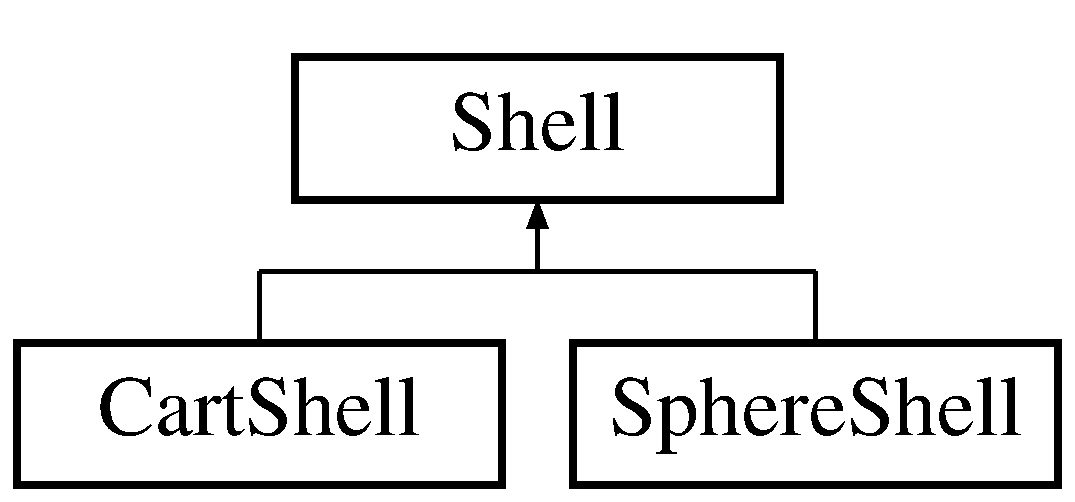
\includegraphics[height=2cm]{classJKBuilder_1_1Shell}
\end{center}
\end{figure}
\subsection*{Public Member Functions}
\begin{DoxyCompactItemize}
\item 
\hyperlink{classJKBuilder_1_1Shell_aaf2d048844f6fbd887a4d915fd25e711}{Shell} (int l\_\-=0, bool isCart=true)
\begin{DoxyCompactList}\small\item\em Creates a \hyperlink{classJKBuilder_1_1Shell}{Shell}. \item\end{DoxyCompactList}\item 
virtual \hyperlink{classJKBuilder_1_1Shell_aafdad0fa9de137c286b786898f3ba361}{$\sim$Shell} ()
\begin{DoxyCompactList}\small\item\em Frees memory associated with the shell. \item\end{DoxyCompactList}\item 
int \hyperlink{classJKBuilder_1_1Shell_abc886cd4e35d3c56a0250b7d06986f61}{GetNPrims} ()
\begin{DoxyCompactList}\small\item\em Returns the number of primitives. \item\end{DoxyCompactList}\item 
int \hyperlink{classJKBuilder_1_1Shell_a7cc8fc5bc043267a7b47e69503e0e308}{GetL} ()
\begin{DoxyCompactList}\small\item\em Returns the angular momentum. \item\end{DoxyCompactList}\item 
bool \hyperlink{classJKBuilder_1_1Shell_a75c22d97e837f5c439eb51aa223bed98}{IsCart} ()
\begin{DoxyCompactList}\small\item\em Returns true if this a Cartesian like shell. \item\end{DoxyCompactList}\item 
virtual int \hyperlink{classJKBuilder_1_1Shell_a1167cdb6f1e1ba08ba6cbffa0b32ca77}{GetNBasis} ()=0
\begin{DoxyCompactList}\small\item\em Returns the number of basis functions in the shell. \item\end{DoxyCompactList}\item 
void \hyperlink{classJKBuilder_1_1Shell_a20ec923cb07d5d3762fffa4501d09924}{AddPrimitive} (double c0, double beta0)
\begin{DoxyCompactList}\small\item\em Creates a primitive with expansion coefficient c0 and exponent scale factor beta0. \item\end{DoxyCompactList}\item 
\hyperlink{classJKBuilder_1_1Primitive}{Primitive} $\ast$ \hyperlink{classJKBuilder_1_1Shell_ae98a68bcb237e53c8c063aded1b34f2e}{operator\mbox{[}$\,$\mbox{]}} (const int i)
\begin{DoxyCompactList}\small\item\em Returns a pointer to the i-\/th primitive. \item\end{DoxyCompactList}\item 
void \hyperlink{classJKBuilder_1_1Shell_a388f572c62279f839ee138a9afbdeeb5}{print} ()
\begin{DoxyCompactList}\small\item\em Prints out the shell. \item\end{DoxyCompactList}\end{DoxyCompactItemize}
\subsection*{Protected Attributes}
\begin{DoxyCompactItemize}
\item 
bool \hyperlink{classJKBuilder_1_1Shell_a8a5f217a40aac0ce092effdd9b6db9f6}{spherical}
\begin{DoxyCompactList}\small\item\em True if spherical, false if Cartesian. \item\end{DoxyCompactList}\item 
int \hyperlink{classJKBuilder_1_1Shell_a89606eca6b563ec68d2da2e84657736f}{l}
\begin{DoxyCompactList}\small\item\em The angular momentum of this shell. \item\end{DoxyCompactList}\item 
std::vector$<$ \hyperlink{classJKBuilder_1_1Primitive}{Primitive} $\ast$ $>$ \hyperlink{classJKBuilder_1_1Shell_afd0049f3a997082e636f4dae72879da2}{gi}
\begin{DoxyCompactList}\small\item\em A vector of the Primitives for this shell. \item\end{DoxyCompactList}\end{DoxyCompactItemize}
\subsection*{Private Member Functions}
\begin{DoxyCompactItemize}
\item 
std::string \hyperlink{classJKBuilder_1_1Shell_abf69d46e0ac3418b1e7926c9e18def95}{l2string} ()
\end{DoxyCompactItemize}


\subsection{Detailed Description}
A shell of Gaussian primitives. Each shell, of momentum $\ell$, is a set of functions $\left\lbrace\phi^{abc}:a+b+c=\ell\right\rbrace$, each of which is assumed of the form:

\[ \phi^{abc}\left(\bf{r}\right)=\left(x-x_0\right)^a\left(y-y_0\right)^b\left(z-z_0\right)^c\sum_i g_i\left(\bf{r}:c_i,\beta_i\right) \]

Note, that the actual member flag controlling whether the shell Cartesian or spherical is true for spherical and false for Cartesian, which is the opposite of how everything outside of the class sees it. For better or for worse, I decided to do it this way so that I could use words with Cart in them and not interfere with the flag. Of course I know also have Cartesian coordinates in the class, so that logic is out the window...

This class is an abstract base class that is the parent to \hyperlink{classJKBuilder_1_1CartShell}{CartShell} and \hyperlink{classJKBuilder_1_1SphereShell}{SphereShell}, which in turn implement the GetNBasis fxn as is appropriate for that type. 

\subsection{Constructor \& Destructor Documentation}
\hypertarget{classJKBuilder_1_1Shell_aaf2d048844f6fbd887a4d915fd25e711}{
\index{JKBuilder::Shell@{JKBuilder::Shell}!Shell@{Shell}}
\index{Shell@{Shell}!JKBuilder::Shell@{JKBuilder::Shell}}
\subsubsection[{Shell}]{\setlength{\rightskip}{0pt plus 5cm}{\bf Shell} (int {\em l\_\-} = {\ttfamily 0}, \/  bool {\em isCart} = {\ttfamily true})}}
\label{classJKBuilder_1_1Shell_aaf2d048844f6fbd887a4d915fd25e711}


Creates a \hyperlink{classJKBuilder_1_1Shell}{Shell}. 
\begin{DoxyParams}{Parameters}
\item[\mbox{$\leftarrow$} {\em l\_\-}]with angular momentum (default is s-\/type) \item[\mbox{$\leftarrow$} {\em isCart}]if true, which is the default, orbitals are Cartesian like, if false, they are spherical like \end{DoxyParams}
\hypertarget{classJKBuilder_1_1Shell_aafdad0fa9de137c286b786898f3ba361}{
\index{JKBuilder::Shell@{JKBuilder::Shell}!$\sim$Shell@{$\sim$Shell}}
\index{$\sim$Shell@{$\sim$Shell}!JKBuilder::Shell@{JKBuilder::Shell}}
\subsubsection[{$\sim$Shell}]{\setlength{\rightskip}{0pt plus 5cm}$\sim${\bf Shell} ()\hspace{0.3cm}{\ttfamily  \mbox{[}virtual\mbox{]}}}}
\label{classJKBuilder_1_1Shell_aafdad0fa9de137c286b786898f3ba361}


Frees memory associated with the shell. 

\subsection{Member Function Documentation}
\hypertarget{classJKBuilder_1_1Shell_abf69d46e0ac3418b1e7926c9e18def95}{
\index{JKBuilder::Shell@{JKBuilder::Shell}!l2string@{l2string}}
\index{l2string@{l2string}!JKBuilder::Shell@{JKBuilder::Shell}}
\subsubsection[{l2string}]{\setlength{\rightskip}{0pt plus 5cm}string l2string ()\hspace{0.3cm}{\ttfamily  \mbox{[}private\mbox{]}}}}
\label{classJKBuilder_1_1Shell_abf69d46e0ac3418b1e7926c9e18def95}
\hypertarget{classJKBuilder_1_1Shell_abc886cd4e35d3c56a0250b7d06986f61}{
\index{JKBuilder::Shell@{JKBuilder::Shell}!GetNPrims@{GetNPrims}}
\index{GetNPrims@{GetNPrims}!JKBuilder::Shell@{JKBuilder::Shell}}
\subsubsection[{GetNPrims}]{\setlength{\rightskip}{0pt plus 5cm}int GetNPrims ()}}
\label{classJKBuilder_1_1Shell_abc886cd4e35d3c56a0250b7d06986f61}


Returns the number of primitives. \hypertarget{classJKBuilder_1_1Shell_a7cc8fc5bc043267a7b47e69503e0e308}{
\index{JKBuilder::Shell@{JKBuilder::Shell}!GetL@{GetL}}
\index{GetL@{GetL}!JKBuilder::Shell@{JKBuilder::Shell}}
\subsubsection[{GetL}]{\setlength{\rightskip}{0pt plus 5cm}int GetL ()}}
\label{classJKBuilder_1_1Shell_a7cc8fc5bc043267a7b47e69503e0e308}


Returns the angular momentum. \hypertarget{classJKBuilder_1_1Shell_a75c22d97e837f5c439eb51aa223bed98}{
\index{JKBuilder::Shell@{JKBuilder::Shell}!IsCart@{IsCart}}
\index{IsCart@{IsCart}!JKBuilder::Shell@{JKBuilder::Shell}}
\subsubsection[{IsCart}]{\setlength{\rightskip}{0pt plus 5cm}bool IsCart ()}}
\label{classJKBuilder_1_1Shell_a75c22d97e837f5c439eb51aa223bed98}


Returns true if this a Cartesian like shell. \hypertarget{classJKBuilder_1_1Shell_a1167cdb6f1e1ba08ba6cbffa0b32ca77}{
\index{JKBuilder::Shell@{JKBuilder::Shell}!GetNBasis@{GetNBasis}}
\index{GetNBasis@{GetNBasis}!JKBuilder::Shell@{JKBuilder::Shell}}
\subsubsection[{GetNBasis}]{\setlength{\rightskip}{0pt plus 5cm}virtual int GetNBasis ()\hspace{0.3cm}{\ttfamily  \mbox{[}pure virtual\mbox{]}}}}
\label{classJKBuilder_1_1Shell_a1167cdb6f1e1ba08ba6cbffa0b32ca77}


Returns the number of basis functions in the shell. 

Implemented in \hyperlink{classJKBuilder_1_1CartShell_a297c144fb990284ac5973c99cdd55f91}{CartShell}, and \hyperlink{classJKBuilder_1_1SphereShell_a297c144fb990284ac5973c99cdd55f91}{SphereShell}.\hypertarget{classJKBuilder_1_1Shell_a20ec923cb07d5d3762fffa4501d09924}{
\index{JKBuilder::Shell@{JKBuilder::Shell}!AddPrimitive@{AddPrimitive}}
\index{AddPrimitive@{AddPrimitive}!JKBuilder::Shell@{JKBuilder::Shell}}
\subsubsection[{AddPrimitive}]{\setlength{\rightskip}{0pt plus 5cm}void AddPrimitive (double {\em c0}, \/  double {\em beta0})}}
\label{classJKBuilder_1_1Shell_a20ec923cb07d5d3762fffa4501d09924}


Creates a primitive with expansion coefficient c0 and exponent scale factor beta0. \hypertarget{classJKBuilder_1_1Shell_ae98a68bcb237e53c8c063aded1b34f2e}{
\index{JKBuilder::Shell@{JKBuilder::Shell}!operator\mbox{[}\mbox{]}@{operator[]}}
\index{operator\mbox{[}\mbox{]}@{operator[]}!JKBuilder::Shell@{JKBuilder::Shell}}
\subsubsection[{operator[]}]{\setlength{\rightskip}{0pt plus 5cm}{\bf Primitive} $\ast$ operator\mbox{[}$\,$\mbox{]} (const int {\em i})}}
\label{classJKBuilder_1_1Shell_ae98a68bcb237e53c8c063aded1b34f2e}


Returns a pointer to the i-\/th primitive. \hypertarget{classJKBuilder_1_1Shell_a388f572c62279f839ee138a9afbdeeb5}{
\index{JKBuilder::Shell@{JKBuilder::Shell}!print@{print}}
\index{print@{print}!JKBuilder::Shell@{JKBuilder::Shell}}
\subsubsection[{print}]{\setlength{\rightskip}{0pt plus 5cm}void print ()}}
\label{classJKBuilder_1_1Shell_a388f572c62279f839ee138a9afbdeeb5}


Prints out the shell. 

\subsection{Member Data Documentation}
\hypertarget{classJKBuilder_1_1Shell_a8a5f217a40aac0ce092effdd9b6db9f6}{
\index{JKBuilder::Shell@{JKBuilder::Shell}!spherical@{spherical}}
\index{spherical@{spherical}!JKBuilder::Shell@{JKBuilder::Shell}}
\subsubsection[{spherical}]{\setlength{\rightskip}{0pt plus 5cm}bool {\bf spherical}\hspace{0.3cm}{\ttfamily  \mbox{[}protected\mbox{]}}}}
\label{classJKBuilder_1_1Shell_a8a5f217a40aac0ce092effdd9b6db9f6}


True if spherical, false if Cartesian. \hypertarget{classJKBuilder_1_1Shell_a89606eca6b563ec68d2da2e84657736f}{
\index{JKBuilder::Shell@{JKBuilder::Shell}!l@{l}}
\index{l@{l}!JKBuilder::Shell@{JKBuilder::Shell}}
\subsubsection[{l}]{\setlength{\rightskip}{0pt plus 5cm}int {\bf l}\hspace{0.3cm}{\ttfamily  \mbox{[}protected\mbox{]}}}}
\label{classJKBuilder_1_1Shell_a89606eca6b563ec68d2da2e84657736f}


The angular momentum of this shell. \hypertarget{classJKBuilder_1_1Shell_afd0049f3a997082e636f4dae72879da2}{
\index{JKBuilder::Shell@{JKBuilder::Shell}!gi@{gi}}
\index{gi@{gi}!JKBuilder::Shell@{JKBuilder::Shell}}
\subsubsection[{gi}]{\setlength{\rightskip}{0pt plus 5cm}std::vector$<${\bf Primitive}$\ast$$>$ {\bf gi}\hspace{0.3cm}{\ttfamily  \mbox{[}protected\mbox{]}}}}
\label{classJKBuilder_1_1Shell_afd0049f3a997082e636f4dae72879da2}


A vector of the Primitives for this shell. 

The documentation for this class was generated from the following files:\begin{DoxyCompactItemize}
\item 
src/\hyperlink{BasisSet_8h}{BasisSet.h}\item 
src/\hyperlink{BasisSet_8cpp}{BasisSet.cpp}\end{DoxyCompactItemize}

\hypertarget{classJKBuilder_1_1ShellPairIterator}{
\section{ShellPairIterator Class Reference}
\label{classJKBuilder_1_1ShellPairIterator}\index{JKBuilder::ShellPairIterator@{JKBuilder::ShellPairIterator}}
}


Iterates over a pair of shells.  


{\ttfamily \#include $<$Iterators.h$>$}Inheritance diagram for ShellPairIterator::\begin{figure}[H]
\begin{center}
\leavevmode
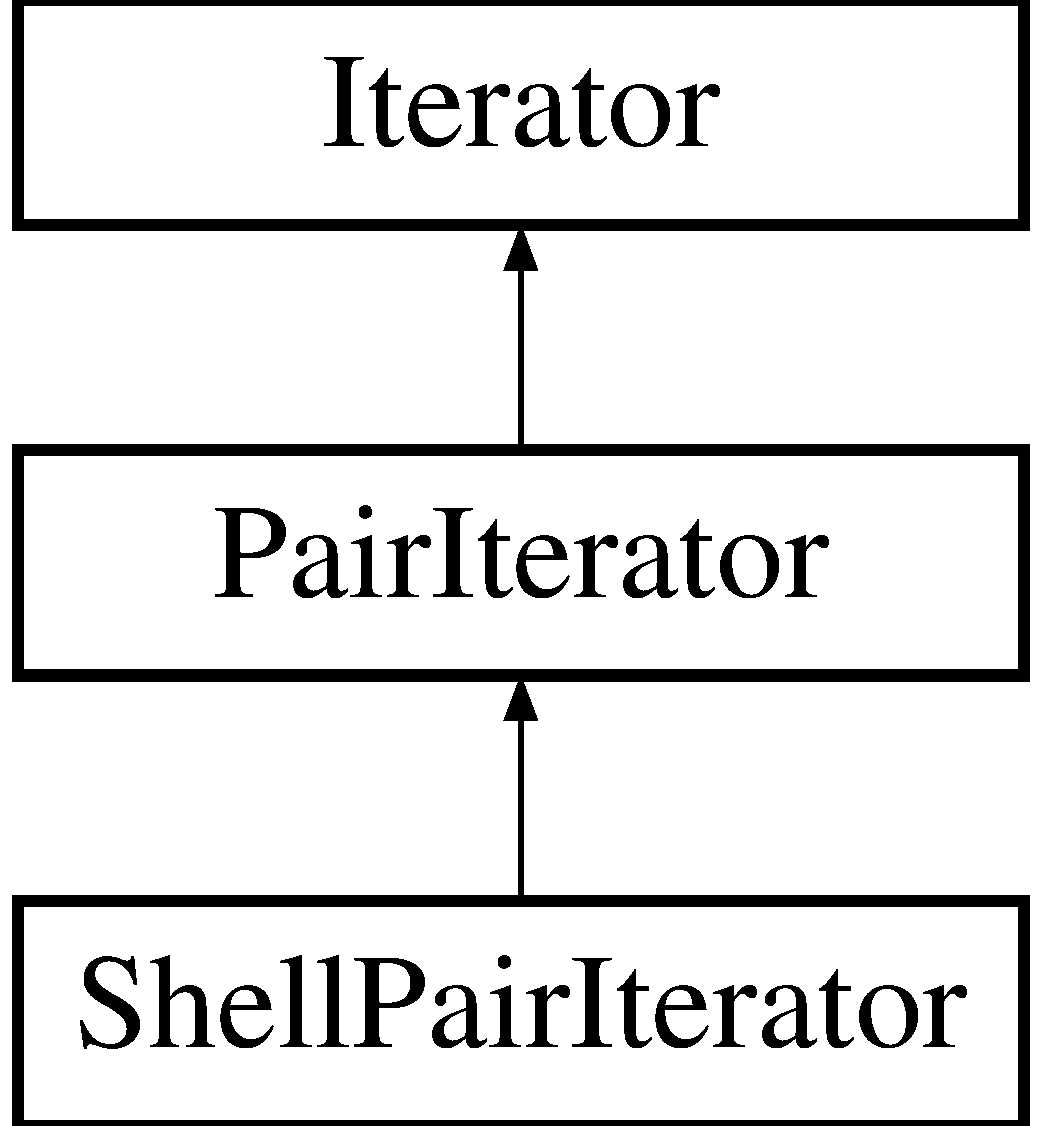
\includegraphics[height=3cm]{classJKBuilder_1_1ShellPairIterator}
\end{center}
\end{figure}
\subsection*{Public Member Functions}
\begin{DoxyCompactItemize}
\item 
\hyperlink{classJKBuilder_1_1ShellPairIterator_a09d264284681ba51a345d1bf04e73a1a}{ShellPairIterator} (\hyperlink{classJKBuilder_1_1ShellPairIterator}{ShellPairIterator} const \&other)
\begin{DoxyCompactList}\small\item\em Makes this shell pair iterator a copy of other. \item\end{DoxyCompactList}\item 
\hyperlink{classJKBuilder_1_1ShellPairIterator_aa348d2d0bd41d0944cf43db3ca6b967f}{ShellPairIterator} (const std::vector$<$ \hyperlink{classJKBuilder_1_1AtomicBasisSet}{AtomicBasisSet} $\ast$ $>$ \&ABSs, int $\ast$Atoms, bool start)
\begin{DoxyCompactList}\small\item\em Given the Atomic basis sets for the two atoms in Atoms makes an iterator (start==true) or the end condition (start==false). \item\end{DoxyCompactList}\item 
virtual \hyperlink{classJKBuilder_1_1ShellPairIterator_a4374ea1e5f0ed1fad10a7c4cf86f6d90}{$\sim$ShellPairIterator} ()
\begin{DoxyCompactList}\small\item\em No memory to free. \item\end{DoxyCompactList}\item 
\hyperlink{classJKBuilder_1_1ShellPairIterator}{ShellPairIterator} \& \hyperlink{classJKBuilder_1_1ShellPairIterator_af3001050bade3a939d83971d1a3f47e7}{operator=} (\hyperlink{classJKBuilder_1_1ShellPairIterator}{ShellPairIterator} const \&other)
\item 
int \hyperlink{classJKBuilder_1_1PairIterator_a370ad37c854fbbf6421ebf9ab35cd027}{ID} (const int i) const 
\begin{DoxyCompactList}\small\item\em Returns the ID of element i of the pair. \item\end{DoxyCompactList}\item 
virtual bool \hyperlink{classJKBuilder_1_1PairIterator_a1984297ca1081efc0513ec2f5e6a6177}{operator$<$} (\hyperlink{classJKBuilder_1_1PairIterator}{PairIterator} const \&other)
\item 
bool \hyperlink{classJKBuilder_1_1PairIterator_a9c95b8dd7929cb34336a944ce96e88a7}{operator$<$=} (\hyperlink{classJKBuilder_1_1PairIterator}{PairIterator} const \&other)
\begin{DoxyCompactList}\small\item\em Returns true if operator$<$ is true or operator== is true. \item\end{DoxyCompactList}\item 
bool \hyperlink{classJKBuilder_1_1PairIterator_ab37a738406950a5e19931f4c09b41f29}{operator$>$} (\hyperlink{classJKBuilder_1_1PairIterator}{PairIterator} const \&other)
\begin{DoxyCompactList}\small\item\em Returns true if operator$<$= is false. \item\end{DoxyCompactList}\item 
bool \hyperlink{classJKBuilder_1_1PairIterator_a0064337d38b8f97d0367be2e9bd31d62}{operator$>$=} (\hyperlink{classJKBuilder_1_1PairIterator}{PairIterator} const \&other)
\begin{DoxyCompactList}\small\item\em Returns true if operator$>$ or operator== is true. \item\end{DoxyCompactList}\item 
bool \hyperlink{classJKBuilder_1_1PairIterator_a6b4e430066f478e5e400edd39ef93968}{operator==} (\hyperlink{classJKBuilder_1_1PairIterator}{PairIterator} const \&other) const 
\item 
virtual void \hyperlink{classJKBuilder_1_1Iterator_a34ca36a99b20ae3170babadaffe51ed2}{Start} (int n=0)
\begin{DoxyCompactList}\small\item\em Returns an iterator suitable for starting on iteration n. \item\end{DoxyCompactList}\item 
virtual void \hyperlink{classJKBuilder_1_1Iterator_a5f692b73d2e160450f4617bb75825e11}{End} (int n=-\/1)
\begin{DoxyCompactList}\small\item\em Returns an iterator representing the state of the iterator after n iterations have occured. \item\end{DoxyCompactList}\item 
\hyperlink{classJKBuilder_1_1Iterator}{Iterator} \hyperlink{classJKBuilder_1_1Iterator_ac1702aedba13b4112b891b58dfd78eba}{operator++} (int)
\begin{DoxyCompactList}\small\item\em Increments the iterator after returning it's value. \item\end{DoxyCompactList}\item 
\hyperlink{classJKBuilder_1_1Iterator}{Iterator} \& \hyperlink{classJKBuilder_1_1Iterator_ae1f21c74128a5ef5d1b9de72ceb09be8}{operator++} ()
\begin{DoxyCompactList}\small\item\em Increments the iterator before returning it's value. \item\end{DoxyCompactList}\item 
bool \hyperlink{classJKBuilder_1_1Iterator_a8c06af8ae0d9d1614ae9f81629275926}{operator!=} (const \hyperlink{classJKBuilder_1_1Iterator}{Iterator} \&other)
\begin{DoxyCompactList}\small\item\em Returns the opposite of operator==. \item\end{DoxyCompactList}\item 
void \hyperlink{classJKBuilder_1_1Iterator_aa83de505e29125c1d3ac7bb1b13ca15a}{SetStart} (std::vector$<$ int $>$ const \&other)
\begin{DoxyCompactList}\small\item\em Sets the N Indices to the N given in other. \item\end{DoxyCompactList}\item 
void \hyperlink{classJKBuilder_1_1Iterator_aad84ec668b5f41210db34c540aaa31fc}{SetEnd} (std::vector$<$ int $>$ const \&other)
\begin{DoxyCompactList}\small\item\em Sets the N MaxInd in other. \item\end{DoxyCompactList}\item 
int \hyperlink{classJKBuilder_1_1Iterator_a74247cf730a06b23fcb1ec64e5596b25}{operator\mbox{[}$\,$\mbox{]}} (const int i) const 
\begin{DoxyCompactList}\small\item\em Returns index i. \item\end{DoxyCompactList}\end{DoxyCompactItemize}
\subsection*{Protected Member Functions}
\begin{DoxyCompactItemize}
\item 
void \hyperlink{classJKBuilder_1_1ShellPairIterator_a7874a07e98b52f4f147cde6f39353bae}{Iterate} ()
\begin{DoxyCompactList}\small\item\em Returns the next valid pair. \item\end{DoxyCompactList}\end{DoxyCompactItemize}
\subsection*{Protected Attributes}
\begin{DoxyCompactItemize}
\item 
int \hyperlink{classJKBuilder_1_1PairIterator_a5c96d22e39dea8044c7caf8c1213e813}{AbsoluteIDs} \mbox{[}2\mbox{]}
\begin{DoxyCompactList}\small\item\em The absolute identity of the system this pair is part of. \item\end{DoxyCompactList}\item 
std::vector$<$ int $>$ \hyperlink{classJKBuilder_1_1Iterator_a20ca24f6d827aba144bb087c4bcb74a0}{CurrentValue}
\begin{DoxyCompactList}\small\item\em The current value. \item\end{DoxyCompactList}\item 
std::vector$<$ int $>$ \hyperlink{classJKBuilder_1_1Iterator_ab6b56d3c4e9353bc938dd6249cde9ca0}{MaxInd}
\begin{DoxyCompactList}\small\item\em This is a vector of length N containing the maximum each index can be. \item\end{DoxyCompactList}\end{DoxyCompactItemize}


\subsection{Detailed Description}
Iterates over a pair of shells. 

\subsection{Constructor \& Destructor Documentation}
\hypertarget{classJKBuilder_1_1ShellPairIterator_a09d264284681ba51a345d1bf04e73a1a}{
\index{JKBuilder::ShellPairIterator@{JKBuilder::ShellPairIterator}!ShellPairIterator@{ShellPairIterator}}
\index{ShellPairIterator@{ShellPairIterator}!JKBuilder::ShellPairIterator@{JKBuilder::ShellPairIterator}}
\subsubsection[{ShellPairIterator}]{\setlength{\rightskip}{0pt plus 5cm}{\bf ShellPairIterator} ({\bf ShellPairIterator} const \& {\em other})}}
\label{classJKBuilder_1_1ShellPairIterator_a09d264284681ba51a345d1bf04e73a1a}


Makes this shell pair iterator a copy of other. \hypertarget{classJKBuilder_1_1ShellPairIterator_aa348d2d0bd41d0944cf43db3ca6b967f}{
\index{JKBuilder::ShellPairIterator@{JKBuilder::ShellPairIterator}!ShellPairIterator@{ShellPairIterator}}
\index{ShellPairIterator@{ShellPairIterator}!JKBuilder::ShellPairIterator@{JKBuilder::ShellPairIterator}}
\subsubsection[{ShellPairIterator}]{\setlength{\rightskip}{0pt plus 5cm}{\bf ShellPairIterator} (const std::vector$<$ {\bf AtomicBasisSet} $\ast$ $>$ \& {\em ABSs}, \/  int $\ast$ {\em Atoms}, \/  bool {\em start})}}
\label{classJKBuilder_1_1ShellPairIterator_aa348d2d0bd41d0944cf43db3ca6b967f}


Given the Atomic basis sets for the two atoms in Atoms makes an iterator (start==true) or the end condition (start==false). \hypertarget{classJKBuilder_1_1ShellPairIterator_a4374ea1e5f0ed1fad10a7c4cf86f6d90}{
\index{JKBuilder::ShellPairIterator@{JKBuilder::ShellPairIterator}!$\sim$ShellPairIterator@{$\sim$ShellPairIterator}}
\index{$\sim$ShellPairIterator@{$\sim$ShellPairIterator}!JKBuilder::ShellPairIterator@{JKBuilder::ShellPairIterator}}
\subsubsection[{$\sim$ShellPairIterator}]{\setlength{\rightskip}{0pt plus 5cm}$\sim${\bf ShellPairIterator} ()\hspace{0.3cm}{\ttfamily  \mbox{[}virtual\mbox{]}}}}
\label{classJKBuilder_1_1ShellPairIterator_a4374ea1e5f0ed1fad10a7c4cf86f6d90}


No memory to free. 

\subsection{Member Function Documentation}
\hypertarget{classJKBuilder_1_1ShellPairIterator_a7874a07e98b52f4f147cde6f39353bae}{
\index{JKBuilder::ShellPairIterator@{JKBuilder::ShellPairIterator}!Iterate@{Iterate}}
\index{Iterate@{Iterate}!JKBuilder::ShellPairIterator@{JKBuilder::ShellPairIterator}}
\subsubsection[{Iterate}]{\setlength{\rightskip}{0pt plus 5cm}void Iterate ()\hspace{0.3cm}{\ttfamily  \mbox{[}protected, virtual\mbox{]}}}}
\label{classJKBuilder_1_1ShellPairIterator_a7874a07e98b52f4f147cde6f39353bae}


Returns the next valid pair. Letting the indices in this pair be P and Q. This returns the next pair that satisfies Q$<$=P 

Reimplemented from \hyperlink{classJKBuilder_1_1PairIterator_a7874a07e98b52f4f147cde6f39353bae}{PairIterator}.\hypertarget{classJKBuilder_1_1ShellPairIterator_af3001050bade3a939d83971d1a3f47e7}{
\index{JKBuilder::ShellPairIterator@{JKBuilder::ShellPairIterator}!operator=@{operator=}}
\index{operator=@{operator=}!JKBuilder::ShellPairIterator@{JKBuilder::ShellPairIterator}}
\subsubsection[{operator=}]{\setlength{\rightskip}{0pt plus 5cm}{\bf ShellPairIterator} \& operator= ({\bf ShellPairIterator} const \& {\em other})}}
\label{classJKBuilder_1_1ShellPairIterator_af3001050bade3a939d83971d1a3f47e7}


Reimplemented from \hyperlink{classJKBuilder_1_1PairIterator_a698aa7b3d6495bd74dcff5b93be868a8}{PairIterator}.\hypertarget{classJKBuilder_1_1PairIterator_a370ad37c854fbbf6421ebf9ab35cd027}{
\index{JKBuilder::ShellPairIterator@{JKBuilder::ShellPairIterator}!ID@{ID}}
\index{ID@{ID}!JKBuilder::ShellPairIterator@{JKBuilder::ShellPairIterator}}
\subsubsection[{ID}]{\setlength{\rightskip}{0pt plus 5cm}int ID (const int {\em i}) const\hspace{0.3cm}{\ttfamily  \mbox{[}inherited\mbox{]}}}}
\label{classJKBuilder_1_1PairIterator_a370ad37c854fbbf6421ebf9ab35cd027}


Returns the ID of element i of the pair. \hypertarget{classJKBuilder_1_1PairIterator_a1984297ca1081efc0513ec2f5e6a6177}{
\index{JKBuilder::ShellPairIterator@{JKBuilder::ShellPairIterator}!operator$<$@{operator$<$}}
\index{operator$<$@{operator$<$}!JKBuilder::ShellPairIterator@{JKBuilder::ShellPairIterator}}
\subsubsection[{operator$<$}]{\setlength{\rightskip}{0pt plus 5cm}bool operator$<$ ({\bf PairIterator} const \& {\em other})\hspace{0.3cm}{\ttfamily  \mbox{[}virtual, inherited\mbox{]}}}}
\label{classJKBuilder_1_1PairIterator_a1984297ca1081efc0513ec2f5e6a6177}
\hypertarget{classJKBuilder_1_1PairIterator_a9c95b8dd7929cb34336a944ce96e88a7}{
\index{JKBuilder::ShellPairIterator@{JKBuilder::ShellPairIterator}!operator$<$=@{operator$<$=}}
\index{operator$<$=@{operator$<$=}!JKBuilder::ShellPairIterator@{JKBuilder::ShellPairIterator}}
\subsubsection[{operator$<$=}]{\setlength{\rightskip}{0pt plus 5cm}bool operator$<$= ({\bf PairIterator} const \& {\em other})\hspace{0.3cm}{\ttfamily  \mbox{[}inherited\mbox{]}}}}
\label{classJKBuilder_1_1PairIterator_a9c95b8dd7929cb34336a944ce96e88a7}


Returns true if operator$<$ is true or operator== is true. \hypertarget{classJKBuilder_1_1PairIterator_ab37a738406950a5e19931f4c09b41f29}{
\index{JKBuilder::ShellPairIterator@{JKBuilder::ShellPairIterator}!operator$>$@{operator$>$}}
\index{operator$>$@{operator$>$}!JKBuilder::ShellPairIterator@{JKBuilder::ShellPairIterator}}
\subsubsection[{operator$>$}]{\setlength{\rightskip}{0pt plus 5cm}bool operator$>$ ({\bf PairIterator} const \& {\em other})\hspace{0.3cm}{\ttfamily  \mbox{[}inherited\mbox{]}}}}
\label{classJKBuilder_1_1PairIterator_ab37a738406950a5e19931f4c09b41f29}


Returns true if operator$<$= is false. \hypertarget{classJKBuilder_1_1PairIterator_a0064337d38b8f97d0367be2e9bd31d62}{
\index{JKBuilder::ShellPairIterator@{JKBuilder::ShellPairIterator}!operator$>$=@{operator$>$=}}
\index{operator$>$=@{operator$>$=}!JKBuilder::ShellPairIterator@{JKBuilder::ShellPairIterator}}
\subsubsection[{operator$>$=}]{\setlength{\rightskip}{0pt plus 5cm}bool operator$>$= ({\bf PairIterator} const \& {\em other})\hspace{0.3cm}{\ttfamily  \mbox{[}inherited\mbox{]}}}}
\label{classJKBuilder_1_1PairIterator_a0064337d38b8f97d0367be2e9bd31d62}


Returns true if operator$>$ or operator== is true. \hypertarget{classJKBuilder_1_1PairIterator_a6b4e430066f478e5e400edd39ef93968}{
\index{JKBuilder::ShellPairIterator@{JKBuilder::ShellPairIterator}!operator==@{operator==}}
\index{operator==@{operator==}!JKBuilder::ShellPairIterator@{JKBuilder::ShellPairIterator}}
\subsubsection[{operator==}]{\setlength{\rightskip}{0pt plus 5cm}bool operator== ({\bf PairIterator} const \& {\em other}) const\hspace{0.3cm}{\ttfamily  \mbox{[}inherited\mbox{]}}}}
\label{classJKBuilder_1_1PairIterator_a6b4e430066f478e5e400edd39ef93968}


Reimplemented from \hyperlink{classJKBuilder_1_1Iterator_a1ea001976a5bc8ae8dc365e2a912b59a}{Iterator}.\hypertarget{classJKBuilder_1_1Iterator_a34ca36a99b20ae3170babadaffe51ed2}{
\index{JKBuilder::ShellPairIterator@{JKBuilder::ShellPairIterator}!Start@{Start}}
\index{Start@{Start}!JKBuilder::ShellPairIterator@{JKBuilder::ShellPairIterator}}
\subsubsection[{Start}]{\setlength{\rightskip}{0pt plus 5cm}void Start (int {\em n} = {\ttfamily 0})\hspace{0.3cm}{\ttfamily  \mbox{[}virtual, inherited\mbox{]}}}}
\label{classJKBuilder_1_1Iterator_a34ca36a99b20ae3170babadaffe51ed2}


Returns an iterator suitable for starting on iteration n. 

Reimplemented in \hyperlink{classJKBuilder_1_1QuartetIterator_a34ca36a99b20ae3170babadaffe51ed2}{QuartetIterator}.\hypertarget{classJKBuilder_1_1Iterator_a5f692b73d2e160450f4617bb75825e11}{
\index{JKBuilder::ShellPairIterator@{JKBuilder::ShellPairIterator}!End@{End}}
\index{End@{End}!JKBuilder::ShellPairIterator@{JKBuilder::ShellPairIterator}}
\subsubsection[{End}]{\setlength{\rightskip}{0pt plus 5cm}void End (int {\em n} = {\ttfamily -\/1})\hspace{0.3cm}{\ttfamily  \mbox{[}virtual, inherited\mbox{]}}}}
\label{classJKBuilder_1_1Iterator_a5f692b73d2e160450f4617bb75825e11}


Returns an iterator representing the state of the iterator after n iterations have occured. The default argument is n=-\/1, which is a flag corresponding to the last iteration of the iterator 

Reimplemented in \hyperlink{classJKBuilder_1_1QuartetIterator_a5f692b73d2e160450f4617bb75825e11}{QuartetIterator}.\hypertarget{classJKBuilder_1_1Iterator_ac1702aedba13b4112b891b58dfd78eba}{
\index{JKBuilder::ShellPairIterator@{JKBuilder::ShellPairIterator}!operator++@{operator++}}
\index{operator++@{operator++}!JKBuilder::ShellPairIterator@{JKBuilder::ShellPairIterator}}
\subsubsection[{operator++}]{\setlength{\rightskip}{0pt plus 5cm}{\bf Iterator} operator++ (int)\hspace{0.3cm}{\ttfamily  \mbox{[}inherited\mbox{]}}}}
\label{classJKBuilder_1_1Iterator_ac1702aedba13b4112b891b58dfd78eba}


Increments the iterator after returning it's value. \hypertarget{classJKBuilder_1_1Iterator_ae1f21c74128a5ef5d1b9de72ceb09be8}{
\index{JKBuilder::ShellPairIterator@{JKBuilder::ShellPairIterator}!operator++@{operator++}}
\index{operator++@{operator++}!JKBuilder::ShellPairIterator@{JKBuilder::ShellPairIterator}}
\subsubsection[{operator++}]{\setlength{\rightskip}{0pt plus 5cm}{\bf Iterator} \& operator++ ()\hspace{0.3cm}{\ttfamily  \mbox{[}inherited\mbox{]}}}}
\label{classJKBuilder_1_1Iterator_ae1f21c74128a5ef5d1b9de72ceb09be8}


Increments the iterator before returning it's value. \hypertarget{classJKBuilder_1_1Iterator_a8c06af8ae0d9d1614ae9f81629275926}{
\index{JKBuilder::ShellPairIterator@{JKBuilder::ShellPairIterator}!operator!=@{operator!=}}
\index{operator!=@{operator!=}!JKBuilder::ShellPairIterator@{JKBuilder::ShellPairIterator}}
\subsubsection[{operator!=}]{\setlength{\rightskip}{0pt plus 5cm}bool operator!= (const {\bf Iterator} \& {\em other})\hspace{0.3cm}{\ttfamily  \mbox{[}inherited\mbox{]}}}}
\label{classJKBuilder_1_1Iterator_a8c06af8ae0d9d1614ae9f81629275926}


Returns the opposite of operator==. \hypertarget{classJKBuilder_1_1Iterator_aa83de505e29125c1d3ac7bb1b13ca15a}{
\index{JKBuilder::ShellPairIterator@{JKBuilder::ShellPairIterator}!SetStart@{SetStart}}
\index{SetStart@{SetStart}!JKBuilder::ShellPairIterator@{JKBuilder::ShellPairIterator}}
\subsubsection[{SetStart}]{\setlength{\rightskip}{0pt plus 5cm}void SetStart (std::vector$<$ int $>$ const \& {\em other})\hspace{0.3cm}{\ttfamily  \mbox{[}inherited\mbox{]}}}}
\label{classJKBuilder_1_1Iterator_aa83de505e29125c1d3ac7bb1b13ca15a}


Sets the N Indices to the N given in other. \hypertarget{classJKBuilder_1_1Iterator_aad84ec668b5f41210db34c540aaa31fc}{
\index{JKBuilder::ShellPairIterator@{JKBuilder::ShellPairIterator}!SetEnd@{SetEnd}}
\index{SetEnd@{SetEnd}!JKBuilder::ShellPairIterator@{JKBuilder::ShellPairIterator}}
\subsubsection[{SetEnd}]{\setlength{\rightskip}{0pt plus 5cm}void SetEnd (std::vector$<$ int $>$ const \& {\em other})\hspace{0.3cm}{\ttfamily  \mbox{[}inherited\mbox{]}}}}
\label{classJKBuilder_1_1Iterator_aad84ec668b5f41210db34c540aaa31fc}


Sets the N MaxInd in other. \hypertarget{classJKBuilder_1_1Iterator_a74247cf730a06b23fcb1ec64e5596b25}{
\index{JKBuilder::ShellPairIterator@{JKBuilder::ShellPairIterator}!operator\mbox{[}\mbox{]}@{operator[]}}
\index{operator\mbox{[}\mbox{]}@{operator[]}!JKBuilder::ShellPairIterator@{JKBuilder::ShellPairIterator}}
\subsubsection[{operator[]}]{\setlength{\rightskip}{0pt plus 5cm}int operator\mbox{[}$\,$\mbox{]} (const int {\em i}) const\hspace{0.3cm}{\ttfamily  \mbox{[}inherited\mbox{]}}}}
\label{classJKBuilder_1_1Iterator_a74247cf730a06b23fcb1ec64e5596b25}


Returns index i. 

\subsection{Member Data Documentation}
\hypertarget{classJKBuilder_1_1PairIterator_a5c96d22e39dea8044c7caf8c1213e813}{
\index{JKBuilder::ShellPairIterator@{JKBuilder::ShellPairIterator}!AbsoluteIDs@{AbsoluteIDs}}
\index{AbsoluteIDs@{AbsoluteIDs}!JKBuilder::ShellPairIterator@{JKBuilder::ShellPairIterator}}
\subsubsection[{AbsoluteIDs}]{\setlength{\rightskip}{0pt plus 5cm}int {\bf AbsoluteIDs}\mbox{[}2\mbox{]}\hspace{0.3cm}{\ttfamily  \mbox{[}protected, inherited\mbox{]}}}}
\label{classJKBuilder_1_1PairIterator_a5c96d22e39dea8044c7caf8c1213e813}


The absolute identity of the system this pair is part of. If this is a pair of atoms set all elements of this to 0 (all atoms are part of the same molecule. If this is a pair of shells set it to the identity of the \hyperlink{classJKBuilder_1_1atom}{atom} the shell is on. \hypertarget{classJKBuilder_1_1Iterator_a20ca24f6d827aba144bb087c4bcb74a0}{
\index{JKBuilder::ShellPairIterator@{JKBuilder::ShellPairIterator}!CurrentValue@{CurrentValue}}
\index{CurrentValue@{CurrentValue}!JKBuilder::ShellPairIterator@{JKBuilder::ShellPairIterator}}
\subsubsection[{CurrentValue}]{\setlength{\rightskip}{0pt plus 5cm}std::vector$<$int$>$ {\bf CurrentValue}\hspace{0.3cm}{\ttfamily  \mbox{[}protected, inherited\mbox{]}}}}
\label{classJKBuilder_1_1Iterator_a20ca24f6d827aba144bb087c4bcb74a0}


The current value. \hypertarget{classJKBuilder_1_1Iterator_ab6b56d3c4e9353bc938dd6249cde9ca0}{
\index{JKBuilder::ShellPairIterator@{JKBuilder::ShellPairIterator}!MaxInd@{MaxInd}}
\index{MaxInd@{MaxInd}!JKBuilder::ShellPairIterator@{JKBuilder::ShellPairIterator}}
\subsubsection[{MaxInd}]{\setlength{\rightskip}{0pt plus 5cm}std::vector$<$int$>$ {\bf MaxInd}\hspace{0.3cm}{\ttfamily  \mbox{[}protected, inherited\mbox{]}}}}
\label{classJKBuilder_1_1Iterator_ab6b56d3c4e9353bc938dd6249cde9ca0}


This is a vector of length N containing the maximum each index can be. 

The documentation for this class was generated from the following files:\begin{DoxyCompactItemize}
\item 
src/\hyperlink{Iterators_8h}{Iterators.h}\item 
src/\hyperlink{Iterator_8cpp}{Iterator.cpp}\end{DoxyCompactItemize}

\hypertarget{classJKBuilder_1_1ShellQuartetIterator}{
\section{ShellQuartetIterator Class Reference}
\label{classJKBuilder_1_1ShellQuartetIterator}\index{JKBuilder::ShellQuartetIterator@{JKBuilder::ShellQuartetIterator}}
}


An iterator that takes advantage of symmetry of the shells.  


{\ttfamily \#include $<$Iterators.h$>$}Inheritance diagram for ShellQuartetIterator::\begin{figure}[H]
\begin{center}
\leavevmode
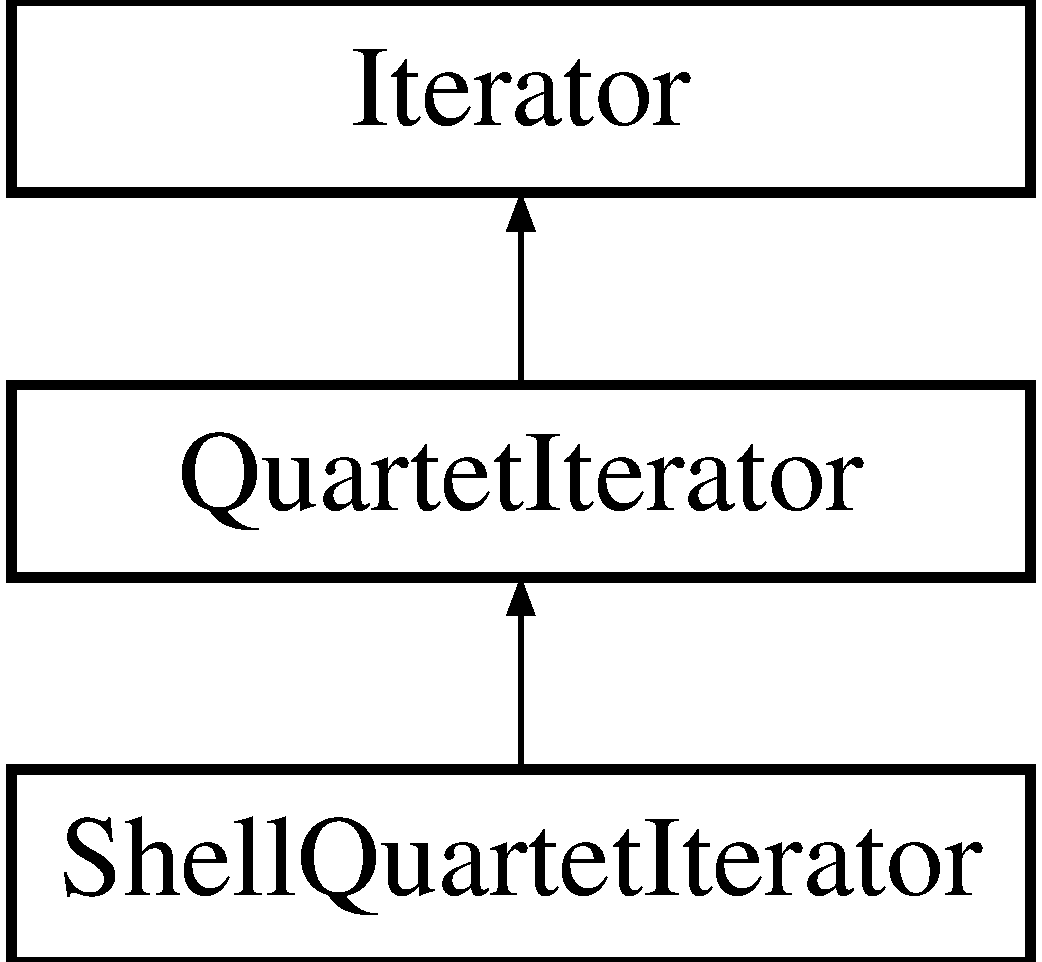
\includegraphics[height=3cm]{classJKBuilder_1_1ShellQuartetIterator}
\end{center}
\end{figure}
\subsection*{Public Member Functions}
\begin{DoxyCompactItemize}
\item 
\hyperlink{classJKBuilder_1_1ShellQuartetIterator_a2b20876856cd8912d9fba4c28428175a}{ShellQuartetIterator} (const std::vector$<$ \hyperlink{classJKBuilder_1_1AtomicBasisSet}{AtomicBasisSet} $\ast$ $>$ \&ABS, int $\ast$Atoms, bool start)
\begin{DoxyCompactList}\small\item\em Makes a new shell quartet iterator (start=true) or the end condition, corresponding to the four Atoms in atoms. \item\end{DoxyCompactList}\item 
\hyperlink{classJKBuilder_1_1ShellQuartetIterator_a6a14b77cf2a987250aa1d25c4e6482a5}{ShellQuartetIterator} (\hyperlink{classJKBuilder_1_1ShellQuartetIterator}{ShellQuartetIterator} const \&other)
\begin{DoxyCompactList}\small\item\em Makes this iterator a copy of other. \item\end{DoxyCompactList}\item 
\hyperlink{classJKBuilder_1_1ShellQuartetIterator}{ShellQuartetIterator} \& \hyperlink{classJKBuilder_1_1ShellQuartetIterator_acd8ac6ed2e831bcb87e65acc0de747db}{operator=} (\hyperlink{classJKBuilder_1_1ShellQuartetIterator}{ShellQuartetIterator} const \&other)
\item 
void \hyperlink{classJKBuilder_1_1QuartetIterator_a34ca36a99b20ae3170babadaffe51ed2}{Start} (int n=0)
\begin{DoxyCompactList}\small\item\em Returns an iterator suitable for starting on iteration n. \item\end{DoxyCompactList}\item 
void \hyperlink{classJKBuilder_1_1QuartetIterator_a5f692b73d2e160450f4617bb75825e11}{End} (int n=-\/1)
\begin{DoxyCompactList}\small\item\em Returns an iterator representing the state of the iterator after n iterations have occured. \item\end{DoxyCompactList}\item 
\hyperlink{classJKBuilder_1_1Iterator}{Iterator} \hyperlink{classJKBuilder_1_1Iterator_ac1702aedba13b4112b891b58dfd78eba}{operator++} (int)
\begin{DoxyCompactList}\small\item\em Increments the iterator after returning it's value. \item\end{DoxyCompactList}\item 
\hyperlink{classJKBuilder_1_1Iterator}{Iterator} \& \hyperlink{classJKBuilder_1_1Iterator_ae1f21c74128a5ef5d1b9de72ceb09be8}{operator++} ()
\begin{DoxyCompactList}\small\item\em Increments the iterator before returning it's value. \item\end{DoxyCompactList}\item 
bool \hyperlink{classJKBuilder_1_1Iterator_a1ea001976a5bc8ae8dc365e2a912b59a}{operator==} (const \hyperlink{classJKBuilder_1_1Iterator}{Iterator} \&other) const 
\item 
bool \hyperlink{classJKBuilder_1_1Iterator_a8c06af8ae0d9d1614ae9f81629275926}{operator!=} (const \hyperlink{classJKBuilder_1_1Iterator}{Iterator} \&other)
\begin{DoxyCompactList}\small\item\em Returns the opposite of operator==. \item\end{DoxyCompactList}\item 
void \hyperlink{classJKBuilder_1_1Iterator_aa83de505e29125c1d3ac7bb1b13ca15a}{SetStart} (std::vector$<$ int $>$ const \&other)
\begin{DoxyCompactList}\small\item\em Sets the N Indices to the N given in other. \item\end{DoxyCompactList}\item 
void \hyperlink{classJKBuilder_1_1Iterator_aad84ec668b5f41210db34c540aaa31fc}{SetEnd} (std::vector$<$ int $>$ const \&other)
\begin{DoxyCompactList}\small\item\em Sets the N MaxInd in other. \item\end{DoxyCompactList}\item 
int \hyperlink{classJKBuilder_1_1Iterator_a74247cf730a06b23fcb1ec64e5596b25}{operator\mbox{[}$\,$\mbox{]}} (const int i) const 
\begin{DoxyCompactList}\small\item\em Returns index i. \item\end{DoxyCompactList}\end{DoxyCompactItemize}
\subsection*{Protected Member Functions}
\begin{DoxyCompactItemize}
\item 
bool \hyperlink{classJKBuilder_1_1ShellQuartetIterator_a458dcf49c4c4bbb1e3d3d39d3dc086c9}{RSIsMaxed} ()
\begin{DoxyCompactList}\small\item\em The definition of what it means for RS to be maxed. \item\end{DoxyCompactList}\item 
bool \hyperlink{classJKBuilder_1_1ShellQuartetIterator_a13e657ea529c0566a0bf48e9c5a488d7}{RSIsOK} ()
\begin{DoxyCompactList}\small\item\em A check to see if the iterated RS value is acceptable. \item\end{DoxyCompactList}\item 
virtual void \hyperlink{classJKBuilder_1_1QuartetIterator_a7874a07e98b52f4f147cde6f39353bae}{Iterate} ()
\item 
void \hyperlink{classJKBuilder_1_1QuartetIterator_a1af5c865d6e9cfe63d0dedc53bdc13ba}{UpdateCurrentValue} ()
\begin{DoxyCompactList}\small\item\em Copies PQ and RS into CurrentValue. \item\end{DoxyCompactList}\end{DoxyCompactItemize}
\subsection*{Protected Attributes}
\begin{DoxyCompactItemize}
\item 
\hyperlink{classJKBuilder_1_1PairIterator}{PairIterator} $\ast$ \hyperlink{classJKBuilder_1_1QuartetIterator_a84f5c3632fba19d3bb85e1cffb9e51f7}{PQ}
\item 
\hyperlink{classJKBuilder_1_1PairIterator}{PairIterator} $\ast$ \hyperlink{classJKBuilder_1_1QuartetIterator_a26b777bf7ea22524f1cc725020ee2082}{RS}
\item 
std::vector$<$ int $>$ \hyperlink{classJKBuilder_1_1Iterator_a20ca24f6d827aba144bb087c4bcb74a0}{CurrentValue}
\begin{DoxyCompactList}\small\item\em The current value. \item\end{DoxyCompactList}\item 
std::vector$<$ int $>$ \hyperlink{classJKBuilder_1_1Iterator_ab6b56d3c4e9353bc938dd6249cde9ca0}{MaxInd}
\begin{DoxyCompactList}\small\item\em This is a vector of length N containing the maximum each index can be. \item\end{DoxyCompactList}\end{DoxyCompactItemize}


\subsection{Detailed Description}
An iterator that takes advantage of symmetry of the shells. For maximum complexity the four-\/index integrals can be thought of as a rank 12 \hyperlink{classJKBuilder_1_1tensor}{tensor}. At the top level it is a rank 4 \hyperlink{classJKBuilder_1_1tensor}{tensor} indexed by atoms, each element in that \hyperlink{classJKBuilder_1_1tensor}{tensor} is a rank 4 \hyperlink{classJKBuilder_1_1tensor}{tensor} indexed by shells, each element in that \hyperlink{classJKBuilder_1_1tensor}{tensor} is a rank 4 \hyperlink{classJKBuilder_1_1tensor}{tensor} indexed by basis functions. We can avoid a lot of calculations because of symmetry of the elements. The \hyperlink{classJKBuilder_1_1ShellQuartetIterator}{ShellQuartetIterator} (SQI) class is invoked by passing four Atomic basis sets and telling it whether you want the resulting iterator to be the starting iterator or the end condition. SQI assumes that the first two atoms will be forming a shell pair and the second two will be forming a shell pair. Calling them atoms P,Q,R, and S respectively, which give shells p,q,r, and s respectively, we know: \begin{eqnarray*} \left(pq|rs\right)=&\left(qp|rs\right)\\ =&\left(pq|sr\right)\\ =&\left(qp|sr\right)\\ =&\left(rs|pq\right)\\ =&\left(sr|pq\right)\\ =&\left(rs|qp\right)\\ =&\left(sr|qp\right), \end{eqnarray*} where the first three, and the last three, equalities follow from the fact that p,q,r and s are real and the fourth follows from the indistinguishability of electrons.

Thinking of each pair, (p,q), as a composite index, whose value, i, is obtained by the mapping $i=p*N_{Shells}+q$ and each pair, (r,s), as a composite index, whose value, j, is obtained by the mapping $j=r*N_{Shells}+s$, where $N_{Shells}$, is the number of shells in the entire molecule, we can enforce the fourth symmetry by not letting j exceeding i. That is we only consider (i,j) pairs: (0,0); (1,0); (1,1); etc... Mandating that we want to count i and j sequentially, i.e. i(j)=0,1,2,... then we need to count q(s) up to $N_{Shells}$, then increment p(r) by one and continue incrementing p(r). This does not account for the first and last three equalities though, which mean that certain values of i and j, specifically values for which p and q, or r and s have been transposed, should not be included in our i and j pairs. Because we are incrementing q and s, before p and r respectively, this means restricting q and s to values less then or equal to p and r, respectively will enforce the remaining symmetry criteria.

The actual implementation is a bit more complicated because we use relative shell indices, e.g. shell 1 on \hyperlink{classJKBuilder_1_1atom}{atom} 2, instead of absolute indices, but the definition of the boolean relation operators for the \hyperlink{classJKBuilder_1_1ShellPairIterator}{ShellPairIterator} hide the vast majority of this additional complexity. 

\subsection{Constructor \& Destructor Documentation}
\hypertarget{classJKBuilder_1_1ShellQuartetIterator_a2b20876856cd8912d9fba4c28428175a}{
\index{JKBuilder::ShellQuartetIterator@{JKBuilder::ShellQuartetIterator}!ShellQuartetIterator@{ShellQuartetIterator}}
\index{ShellQuartetIterator@{ShellQuartetIterator}!JKBuilder::ShellQuartetIterator@{JKBuilder::ShellQuartetIterator}}
\subsubsection[{ShellQuartetIterator}]{\setlength{\rightskip}{0pt plus 5cm}{\bf ShellQuartetIterator} (const std::vector$<$ {\bf AtomicBasisSet} $\ast$ $>$ \& {\em ABS}, \/  int $\ast$ {\em Atoms}, \/  bool {\em start})}}
\label{classJKBuilder_1_1ShellQuartetIterator_a2b20876856cd8912d9fba4c28428175a}


Makes a new shell quartet iterator (start=true) or the end condition, corresponding to the four Atoms in atoms. \hypertarget{classJKBuilder_1_1ShellQuartetIterator_a6a14b77cf2a987250aa1d25c4e6482a5}{
\index{JKBuilder::ShellQuartetIterator@{JKBuilder::ShellQuartetIterator}!ShellQuartetIterator@{ShellQuartetIterator}}
\index{ShellQuartetIterator@{ShellQuartetIterator}!JKBuilder::ShellQuartetIterator@{JKBuilder::ShellQuartetIterator}}
\subsubsection[{ShellQuartetIterator}]{\setlength{\rightskip}{0pt plus 5cm}{\bf ShellQuartetIterator} ({\bf ShellQuartetIterator} const \& {\em other})}}
\label{classJKBuilder_1_1ShellQuartetIterator_a6a14b77cf2a987250aa1d25c4e6482a5}


Makes this iterator a copy of other. 

\subsection{Member Function Documentation}
\hypertarget{classJKBuilder_1_1ShellQuartetIterator_a458dcf49c4c4bbb1e3d3d39d3dc086c9}{
\index{JKBuilder::ShellQuartetIterator@{JKBuilder::ShellQuartetIterator}!RSIsMaxed@{RSIsMaxed}}
\index{RSIsMaxed@{RSIsMaxed}!JKBuilder::ShellQuartetIterator@{JKBuilder::ShellQuartetIterator}}
\subsubsection[{RSIsMaxed}]{\setlength{\rightskip}{0pt plus 5cm}bool RSIsMaxed ()\hspace{0.3cm}{\ttfamily  \mbox{[}protected, virtual\mbox{]}}}}
\label{classJKBuilder_1_1ShellQuartetIterator_a458dcf49c4c4bbb1e3d3d39d3dc086c9}


The definition of what it means for RS to be maxed. 

Implements \hyperlink{classJKBuilder_1_1QuartetIterator_af88c46759ac710bbd36c17601dc62d55}{QuartetIterator}.\hypertarget{classJKBuilder_1_1ShellQuartetIterator_a13e657ea529c0566a0bf48e9c5a488d7}{
\index{JKBuilder::ShellQuartetIterator@{JKBuilder::ShellQuartetIterator}!RSIsOK@{RSIsOK}}
\index{RSIsOK@{RSIsOK}!JKBuilder::ShellQuartetIterator@{JKBuilder::ShellQuartetIterator}}
\subsubsection[{RSIsOK}]{\setlength{\rightskip}{0pt plus 5cm}bool RSIsOK ()\hspace{0.3cm}{\ttfamily  \mbox{[}protected, virtual\mbox{]}}}}
\label{classJKBuilder_1_1ShellQuartetIterator_a13e657ea529c0566a0bf48e9c5a488d7}


A check to see if the iterated RS value is acceptable. 

Implements \hyperlink{classJKBuilder_1_1QuartetIterator_ac51ff9a02f4a201598f7820476c52faf}{QuartetIterator}.\hypertarget{classJKBuilder_1_1ShellQuartetIterator_acd8ac6ed2e831bcb87e65acc0de747db}{
\index{JKBuilder::ShellQuartetIterator@{JKBuilder::ShellQuartetIterator}!operator=@{operator=}}
\index{operator=@{operator=}!JKBuilder::ShellQuartetIterator@{JKBuilder::ShellQuartetIterator}}
\subsubsection[{operator=}]{\setlength{\rightskip}{0pt plus 5cm}{\bf ShellQuartetIterator} \& operator= ({\bf ShellQuartetIterator} const \& {\em other})}}
\label{classJKBuilder_1_1ShellQuartetIterator_acd8ac6ed2e831bcb87e65acc0de747db}


Reimplemented from \hyperlink{classJKBuilder_1_1QuartetIterator_ab3cd17222545586596dbbc6aa3ca7046}{QuartetIterator}.\hypertarget{classJKBuilder_1_1QuartetIterator_a7874a07e98b52f4f147cde6f39353bae}{
\index{JKBuilder::ShellQuartetIterator@{JKBuilder::ShellQuartetIterator}!Iterate@{Iterate}}
\index{Iterate@{Iterate}!JKBuilder::ShellQuartetIterator@{JKBuilder::ShellQuartetIterator}}
\subsubsection[{Iterate}]{\setlength{\rightskip}{0pt plus 5cm}void Iterate ()\hspace{0.3cm}{\ttfamily  \mbox{[}protected, virtual, inherited\mbox{]}}}}
\label{classJKBuilder_1_1QuartetIterator_a7874a07e98b52f4f147cde6f39353bae}


Reimplemented from \hyperlink{classJKBuilder_1_1Iterator_a7874a07e98b52f4f147cde6f39353bae}{Iterator}.\hypertarget{classJKBuilder_1_1QuartetIterator_a1af5c865d6e9cfe63d0dedc53bdc13ba}{
\index{JKBuilder::ShellQuartetIterator@{JKBuilder::ShellQuartetIterator}!UpdateCurrentValue@{UpdateCurrentValue}}
\index{UpdateCurrentValue@{UpdateCurrentValue}!JKBuilder::ShellQuartetIterator@{JKBuilder::ShellQuartetIterator}}
\subsubsection[{UpdateCurrentValue}]{\setlength{\rightskip}{0pt plus 5cm}void UpdateCurrentValue ()\hspace{0.3cm}{\ttfamily  \mbox{[}protected, inherited\mbox{]}}}}
\label{classJKBuilder_1_1QuartetIterator_a1af5c865d6e9cfe63d0dedc53bdc13ba}


Copies PQ and RS into CurrentValue. \hypertarget{classJKBuilder_1_1QuartetIterator_a34ca36a99b20ae3170babadaffe51ed2}{
\index{JKBuilder::ShellQuartetIterator@{JKBuilder::ShellQuartetIterator}!Start@{Start}}
\index{Start@{Start}!JKBuilder::ShellQuartetIterator@{JKBuilder::ShellQuartetIterator}}
\subsubsection[{Start}]{\setlength{\rightskip}{0pt plus 5cm}void Start (int {\em n} = {\ttfamily 0})\hspace{0.3cm}{\ttfamily  \mbox{[}virtual, inherited\mbox{]}}}}
\label{classJKBuilder_1_1QuartetIterator_a34ca36a99b20ae3170babadaffe51ed2}


Returns an iterator suitable for starting on iteration n. 

Reimplemented from \hyperlink{classJKBuilder_1_1Iterator_a34ca36a99b20ae3170babadaffe51ed2}{Iterator}.\hypertarget{classJKBuilder_1_1QuartetIterator_a5f692b73d2e160450f4617bb75825e11}{
\index{JKBuilder::ShellQuartetIterator@{JKBuilder::ShellQuartetIterator}!End@{End}}
\index{End@{End}!JKBuilder::ShellQuartetIterator@{JKBuilder::ShellQuartetIterator}}
\subsubsection[{End}]{\setlength{\rightskip}{0pt plus 5cm}void End (int {\em n} = {\ttfamily -\/1})\hspace{0.3cm}{\ttfamily  \mbox{[}virtual, inherited\mbox{]}}}}
\label{classJKBuilder_1_1QuartetIterator_a5f692b73d2e160450f4617bb75825e11}


Returns an iterator representing the state of the iterator after n iterations have occured. The default argument is n=-\/1, which is a flag corresponding to the last iteration of the iterator 

Reimplemented from \hyperlink{classJKBuilder_1_1Iterator_a5f692b73d2e160450f4617bb75825e11}{Iterator}.\hypertarget{classJKBuilder_1_1Iterator_ac1702aedba13b4112b891b58dfd78eba}{
\index{JKBuilder::ShellQuartetIterator@{JKBuilder::ShellQuartetIterator}!operator++@{operator++}}
\index{operator++@{operator++}!JKBuilder::ShellQuartetIterator@{JKBuilder::ShellQuartetIterator}}
\subsubsection[{operator++}]{\setlength{\rightskip}{0pt plus 5cm}{\bf Iterator} operator++ (int)\hspace{0.3cm}{\ttfamily  \mbox{[}inherited\mbox{]}}}}
\label{classJKBuilder_1_1Iterator_ac1702aedba13b4112b891b58dfd78eba}


Increments the iterator after returning it's value. \hypertarget{classJKBuilder_1_1Iterator_ae1f21c74128a5ef5d1b9de72ceb09be8}{
\index{JKBuilder::ShellQuartetIterator@{JKBuilder::ShellQuartetIterator}!operator++@{operator++}}
\index{operator++@{operator++}!JKBuilder::ShellQuartetIterator@{JKBuilder::ShellQuartetIterator}}
\subsubsection[{operator++}]{\setlength{\rightskip}{0pt plus 5cm}{\bf Iterator} \& operator++ ()\hspace{0.3cm}{\ttfamily  \mbox{[}inherited\mbox{]}}}}
\label{classJKBuilder_1_1Iterator_ae1f21c74128a5ef5d1b9de72ceb09be8}


Increments the iterator before returning it's value. \hypertarget{classJKBuilder_1_1Iterator_a1ea001976a5bc8ae8dc365e2a912b59a}{
\index{JKBuilder::ShellQuartetIterator@{JKBuilder::ShellQuartetIterator}!operator==@{operator==}}
\index{operator==@{operator==}!JKBuilder::ShellQuartetIterator@{JKBuilder::ShellQuartetIterator}}
\subsubsection[{operator==}]{\setlength{\rightskip}{0pt plus 5cm}bool operator== (const {\bf Iterator} \& {\em other}) const\hspace{0.3cm}{\ttfamily  \mbox{[}inherited\mbox{]}}}}
\label{classJKBuilder_1_1Iterator_a1ea001976a5bc8ae8dc365e2a912b59a}


Reimplemented in \hyperlink{classJKBuilder_1_1PairIterator_a6b4e430066f478e5e400edd39ef93968}{PairIterator}.\hypertarget{classJKBuilder_1_1Iterator_a8c06af8ae0d9d1614ae9f81629275926}{
\index{JKBuilder::ShellQuartetIterator@{JKBuilder::ShellQuartetIterator}!operator!=@{operator!=}}
\index{operator!=@{operator!=}!JKBuilder::ShellQuartetIterator@{JKBuilder::ShellQuartetIterator}}
\subsubsection[{operator!=}]{\setlength{\rightskip}{0pt plus 5cm}bool operator!= (const {\bf Iterator} \& {\em other})\hspace{0.3cm}{\ttfamily  \mbox{[}inherited\mbox{]}}}}
\label{classJKBuilder_1_1Iterator_a8c06af8ae0d9d1614ae9f81629275926}


Returns the opposite of operator==. \hypertarget{classJKBuilder_1_1Iterator_aa83de505e29125c1d3ac7bb1b13ca15a}{
\index{JKBuilder::ShellQuartetIterator@{JKBuilder::ShellQuartetIterator}!SetStart@{SetStart}}
\index{SetStart@{SetStart}!JKBuilder::ShellQuartetIterator@{JKBuilder::ShellQuartetIterator}}
\subsubsection[{SetStart}]{\setlength{\rightskip}{0pt plus 5cm}void SetStart (std::vector$<$ int $>$ const \& {\em other})\hspace{0.3cm}{\ttfamily  \mbox{[}inherited\mbox{]}}}}
\label{classJKBuilder_1_1Iterator_aa83de505e29125c1d3ac7bb1b13ca15a}


Sets the N Indices to the N given in other. \hypertarget{classJKBuilder_1_1Iterator_aad84ec668b5f41210db34c540aaa31fc}{
\index{JKBuilder::ShellQuartetIterator@{JKBuilder::ShellQuartetIterator}!SetEnd@{SetEnd}}
\index{SetEnd@{SetEnd}!JKBuilder::ShellQuartetIterator@{JKBuilder::ShellQuartetIterator}}
\subsubsection[{SetEnd}]{\setlength{\rightskip}{0pt plus 5cm}void SetEnd (std::vector$<$ int $>$ const \& {\em other})\hspace{0.3cm}{\ttfamily  \mbox{[}inherited\mbox{]}}}}
\label{classJKBuilder_1_1Iterator_aad84ec668b5f41210db34c540aaa31fc}


Sets the N MaxInd in other. \hypertarget{classJKBuilder_1_1Iterator_a74247cf730a06b23fcb1ec64e5596b25}{
\index{JKBuilder::ShellQuartetIterator@{JKBuilder::ShellQuartetIterator}!operator\mbox{[}\mbox{]}@{operator[]}}
\index{operator\mbox{[}\mbox{]}@{operator[]}!JKBuilder::ShellQuartetIterator@{JKBuilder::ShellQuartetIterator}}
\subsubsection[{operator[]}]{\setlength{\rightskip}{0pt plus 5cm}int operator\mbox{[}$\,$\mbox{]} (const int {\em i}) const\hspace{0.3cm}{\ttfamily  \mbox{[}inherited\mbox{]}}}}
\label{classJKBuilder_1_1Iterator_a74247cf730a06b23fcb1ec64e5596b25}


Returns index i. 

\subsection{Member Data Documentation}
\hypertarget{classJKBuilder_1_1QuartetIterator_a84f5c3632fba19d3bb85e1cffb9e51f7}{
\index{JKBuilder::ShellQuartetIterator@{JKBuilder::ShellQuartetIterator}!PQ@{PQ}}
\index{PQ@{PQ}!JKBuilder::ShellQuartetIterator@{JKBuilder::ShellQuartetIterator}}
\subsubsection[{PQ}]{\setlength{\rightskip}{0pt plus 5cm}{\bf PairIterator}$\ast$ {\bf PQ}\hspace{0.3cm}{\ttfamily  \mbox{[}protected, inherited\mbox{]}}}}
\label{classJKBuilder_1_1QuartetIterator_a84f5c3632fba19d3bb85e1cffb9e51f7}
\hypertarget{classJKBuilder_1_1QuartetIterator_a26b777bf7ea22524f1cc725020ee2082}{
\index{JKBuilder::ShellQuartetIterator@{JKBuilder::ShellQuartetIterator}!RS@{RS}}
\index{RS@{RS}!JKBuilder::ShellQuartetIterator@{JKBuilder::ShellQuartetIterator}}
\subsubsection[{RS}]{\setlength{\rightskip}{0pt plus 5cm}{\bf PairIterator}$\ast$ {\bf RS}\hspace{0.3cm}{\ttfamily  \mbox{[}protected, inherited\mbox{]}}}}
\label{classJKBuilder_1_1QuartetIterator_a26b777bf7ea22524f1cc725020ee2082}
\hypertarget{classJKBuilder_1_1Iterator_a20ca24f6d827aba144bb087c4bcb74a0}{
\index{JKBuilder::ShellQuartetIterator@{JKBuilder::ShellQuartetIterator}!CurrentValue@{CurrentValue}}
\index{CurrentValue@{CurrentValue}!JKBuilder::ShellQuartetIterator@{JKBuilder::ShellQuartetIterator}}
\subsubsection[{CurrentValue}]{\setlength{\rightskip}{0pt plus 5cm}std::vector$<$int$>$ {\bf CurrentValue}\hspace{0.3cm}{\ttfamily  \mbox{[}protected, inherited\mbox{]}}}}
\label{classJKBuilder_1_1Iterator_a20ca24f6d827aba144bb087c4bcb74a0}


The current value. \hypertarget{classJKBuilder_1_1Iterator_ab6b56d3c4e9353bc938dd6249cde9ca0}{
\index{JKBuilder::ShellQuartetIterator@{JKBuilder::ShellQuartetIterator}!MaxInd@{MaxInd}}
\index{MaxInd@{MaxInd}!JKBuilder::ShellQuartetIterator@{JKBuilder::ShellQuartetIterator}}
\subsubsection[{MaxInd}]{\setlength{\rightskip}{0pt plus 5cm}std::vector$<$int$>$ {\bf MaxInd}\hspace{0.3cm}{\ttfamily  \mbox{[}protected, inherited\mbox{]}}}}
\label{classJKBuilder_1_1Iterator_ab6b56d3c4e9353bc938dd6249cde9ca0}


This is a vector of length N containing the maximum each index can be. 

The documentation for this class was generated from the following files:\begin{DoxyCompactItemize}
\item 
src/\hyperlink{Iterators_8h}{Iterators.h}\item 
src/\hyperlink{Iterator_8cpp}{Iterator.cpp}\end{DoxyCompactItemize}

\hypertarget{classJKBuilder_1_1SphereShell}{
\section{SphereShell Class Reference}
\label{classJKBuilder_1_1SphereShell}\index{JKBuilder::SphereShell@{JKBuilder::SphereShell}}
}


Specialization of \hyperlink{classJKBuilder_1_1Shell}{Shell} to Spherical Gaussians.  


{\ttfamily \#include $<$BasisSet.h$>$}Inheritance diagram for SphereShell::\begin{figure}[H]
\begin{center}
\leavevmode
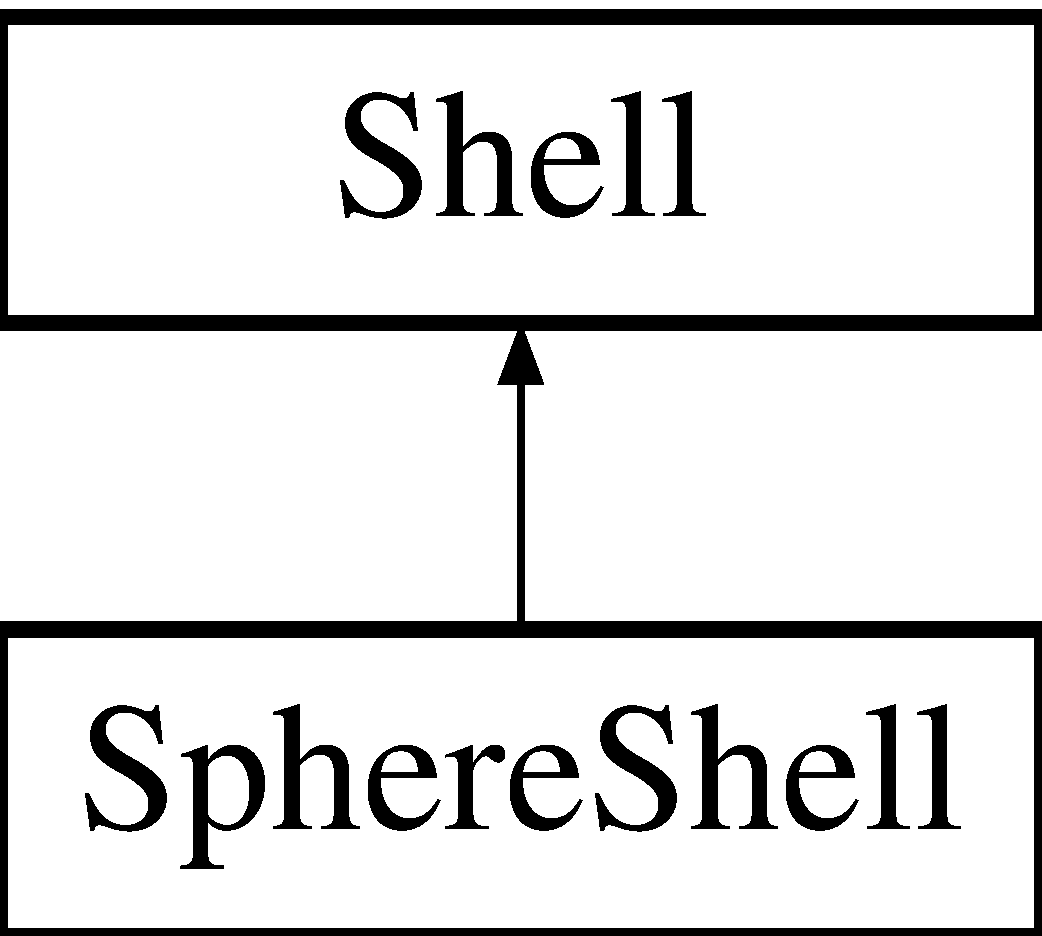
\includegraphics[height=2cm]{classJKBuilder_1_1SphereShell}
\end{center}
\end{figure}
\subsection*{Public Member Functions}
\begin{DoxyCompactItemize}
\item 
\hyperlink{classJKBuilder_1_1SphereShell_af92e2c0e6f04dbf41105b543a6eebdcd}{SphereShell} (int \hyperlink{classJKBuilder_1_1Shell_a89606eca6b563ec68d2da2e84657736f}{l}=0)
\begin{DoxyCompactList}\small\item\em Calls \hyperlink{classJKBuilder_1_1Shell}{Shell} constructor with IsCart=false. \item\end{DoxyCompactList}\item 
int \hyperlink{classJKBuilder_1_1SphereShell_a297c144fb990284ac5973c99cdd55f91}{GetNBasis} ()
\begin{DoxyCompactList}\small\item\em Returns the number of basis functions. \item\end{DoxyCompactList}\item 
int \hyperlink{classJKBuilder_1_1Shell_abc886cd4e35d3c56a0250b7d06986f61}{GetNPrims} ()
\begin{DoxyCompactList}\small\item\em Returns the number of primitives. \item\end{DoxyCompactList}\item 
int \hyperlink{classJKBuilder_1_1Shell_a7cc8fc5bc043267a7b47e69503e0e308}{GetL} ()
\begin{DoxyCompactList}\small\item\em Returns the angular momentum. \item\end{DoxyCompactList}\item 
bool \hyperlink{classJKBuilder_1_1Shell_a75c22d97e837f5c439eb51aa223bed98}{IsCart} ()
\begin{DoxyCompactList}\small\item\em Returns true if this a Cartesian like shell. \item\end{DoxyCompactList}\item 
void \hyperlink{classJKBuilder_1_1Shell_a20ec923cb07d5d3762fffa4501d09924}{AddPrimitive} (double c0, double beta0)
\begin{DoxyCompactList}\small\item\em Creates a primitive with expansion coefficient c0 and exponent scale factor beta0. \item\end{DoxyCompactList}\item 
\hyperlink{classJKBuilder_1_1Primitive}{Primitive} $\ast$ \hyperlink{classJKBuilder_1_1Shell_ae98a68bcb237e53c8c063aded1b34f2e}{operator\mbox{[}$\,$\mbox{]}} (const int i)
\begin{DoxyCompactList}\small\item\em Returns a pointer to the i-\/th primitive. \item\end{DoxyCompactList}\item 
void \hyperlink{classJKBuilder_1_1Shell_a388f572c62279f839ee138a9afbdeeb5}{print} ()
\begin{DoxyCompactList}\small\item\em Prints out the shell. \item\end{DoxyCompactList}\end{DoxyCompactItemize}
\subsection*{Protected Attributes}
\begin{DoxyCompactItemize}
\item 
bool \hyperlink{classJKBuilder_1_1Shell_a8a5f217a40aac0ce092effdd9b6db9f6}{spherical}
\begin{DoxyCompactList}\small\item\em True if spherical, false if Cartesian. \item\end{DoxyCompactList}\item 
int \hyperlink{classJKBuilder_1_1Shell_a89606eca6b563ec68d2da2e84657736f}{l}
\begin{DoxyCompactList}\small\item\em The angular momentum of this shell. \item\end{DoxyCompactList}\item 
std::vector$<$ \hyperlink{classJKBuilder_1_1Primitive}{Primitive} $\ast$ $>$ \hyperlink{classJKBuilder_1_1Shell_afd0049f3a997082e636f4dae72879da2}{gi}
\begin{DoxyCompactList}\small\item\em A vector of the Primitives for this shell. \item\end{DoxyCompactList}\end{DoxyCompactItemize}


\subsection{Detailed Description}
Specialization of \hyperlink{classJKBuilder_1_1Shell}{Shell} to Spherical Gaussians. A shell of spherical Gaussians is characterized by a momentum $\ell$ and has one Gaussian for each value in the set $\lbrace i:0\le |i|\le\ell\rbrace$, which amounts to $2\ell+1$ allowed values. 

\subsection{Constructor \& Destructor Documentation}
\hypertarget{classJKBuilder_1_1SphereShell_af92e2c0e6f04dbf41105b543a6eebdcd}{
\index{JKBuilder::SphereShell@{JKBuilder::SphereShell}!SphereShell@{SphereShell}}
\index{SphereShell@{SphereShell}!JKBuilder::SphereShell@{JKBuilder::SphereShell}}
\subsubsection[{SphereShell}]{\setlength{\rightskip}{0pt plus 5cm}{\bf SphereShell} (int {\em l} = {\ttfamily 0})}}
\label{classJKBuilder_1_1SphereShell_af92e2c0e6f04dbf41105b543a6eebdcd}


Calls \hyperlink{classJKBuilder_1_1Shell}{Shell} constructor with IsCart=false. 

\subsection{Member Function Documentation}
\hypertarget{classJKBuilder_1_1SphereShell_a297c144fb990284ac5973c99cdd55f91}{
\index{JKBuilder::SphereShell@{JKBuilder::SphereShell}!GetNBasis@{GetNBasis}}
\index{GetNBasis@{GetNBasis}!JKBuilder::SphereShell@{JKBuilder::SphereShell}}
\subsubsection[{GetNBasis}]{\setlength{\rightskip}{0pt plus 5cm}int GetNBasis ()\hspace{0.3cm}{\ttfamily  \mbox{[}virtual\mbox{]}}}}
\label{classJKBuilder_1_1SphereShell_a297c144fb990284ac5973c99cdd55f91}


Returns the number of basis functions. 

Implements \hyperlink{classJKBuilder_1_1Shell_a1167cdb6f1e1ba08ba6cbffa0b32ca77}{Shell}.\hypertarget{classJKBuilder_1_1Shell_abc886cd4e35d3c56a0250b7d06986f61}{
\index{JKBuilder::SphereShell@{JKBuilder::SphereShell}!GetNPrims@{GetNPrims}}
\index{GetNPrims@{GetNPrims}!JKBuilder::SphereShell@{JKBuilder::SphereShell}}
\subsubsection[{GetNPrims}]{\setlength{\rightskip}{0pt plus 5cm}int GetNPrims ()\hspace{0.3cm}{\ttfamily  \mbox{[}inherited\mbox{]}}}}
\label{classJKBuilder_1_1Shell_abc886cd4e35d3c56a0250b7d06986f61}


Returns the number of primitives. \hypertarget{classJKBuilder_1_1Shell_a7cc8fc5bc043267a7b47e69503e0e308}{
\index{JKBuilder::SphereShell@{JKBuilder::SphereShell}!GetL@{GetL}}
\index{GetL@{GetL}!JKBuilder::SphereShell@{JKBuilder::SphereShell}}
\subsubsection[{GetL}]{\setlength{\rightskip}{0pt plus 5cm}int GetL ()\hspace{0.3cm}{\ttfamily  \mbox{[}inherited\mbox{]}}}}
\label{classJKBuilder_1_1Shell_a7cc8fc5bc043267a7b47e69503e0e308}


Returns the angular momentum. \hypertarget{classJKBuilder_1_1Shell_a75c22d97e837f5c439eb51aa223bed98}{
\index{JKBuilder::SphereShell@{JKBuilder::SphereShell}!IsCart@{IsCart}}
\index{IsCart@{IsCart}!JKBuilder::SphereShell@{JKBuilder::SphereShell}}
\subsubsection[{IsCart}]{\setlength{\rightskip}{0pt plus 5cm}bool IsCart ()\hspace{0.3cm}{\ttfamily  \mbox{[}inherited\mbox{]}}}}
\label{classJKBuilder_1_1Shell_a75c22d97e837f5c439eb51aa223bed98}


Returns true if this a Cartesian like shell. \hypertarget{classJKBuilder_1_1Shell_a20ec923cb07d5d3762fffa4501d09924}{
\index{JKBuilder::SphereShell@{JKBuilder::SphereShell}!AddPrimitive@{AddPrimitive}}
\index{AddPrimitive@{AddPrimitive}!JKBuilder::SphereShell@{JKBuilder::SphereShell}}
\subsubsection[{AddPrimitive}]{\setlength{\rightskip}{0pt plus 5cm}void AddPrimitive (double {\em c0}, \/  double {\em beta0})\hspace{0.3cm}{\ttfamily  \mbox{[}inherited\mbox{]}}}}
\label{classJKBuilder_1_1Shell_a20ec923cb07d5d3762fffa4501d09924}


Creates a primitive with expansion coefficient c0 and exponent scale factor beta0. \hypertarget{classJKBuilder_1_1Shell_ae98a68bcb237e53c8c063aded1b34f2e}{
\index{JKBuilder::SphereShell@{JKBuilder::SphereShell}!operator\mbox{[}\mbox{]}@{operator[]}}
\index{operator\mbox{[}\mbox{]}@{operator[]}!JKBuilder::SphereShell@{JKBuilder::SphereShell}}
\subsubsection[{operator[]}]{\setlength{\rightskip}{0pt plus 5cm}{\bf Primitive} $\ast$ operator\mbox{[}$\,$\mbox{]} (const int {\em i})\hspace{0.3cm}{\ttfamily  \mbox{[}inherited\mbox{]}}}}
\label{classJKBuilder_1_1Shell_ae98a68bcb237e53c8c063aded1b34f2e}


Returns a pointer to the i-\/th primitive. \hypertarget{classJKBuilder_1_1Shell_a388f572c62279f839ee138a9afbdeeb5}{
\index{JKBuilder::SphereShell@{JKBuilder::SphereShell}!print@{print}}
\index{print@{print}!JKBuilder::SphereShell@{JKBuilder::SphereShell}}
\subsubsection[{print}]{\setlength{\rightskip}{0pt plus 5cm}void print ()\hspace{0.3cm}{\ttfamily  \mbox{[}inherited\mbox{]}}}}
\label{classJKBuilder_1_1Shell_a388f572c62279f839ee138a9afbdeeb5}


Prints out the shell. 

\subsection{Member Data Documentation}
\hypertarget{classJKBuilder_1_1Shell_a8a5f217a40aac0ce092effdd9b6db9f6}{
\index{JKBuilder::SphereShell@{JKBuilder::SphereShell}!spherical@{spherical}}
\index{spherical@{spherical}!JKBuilder::SphereShell@{JKBuilder::SphereShell}}
\subsubsection[{spherical}]{\setlength{\rightskip}{0pt plus 5cm}bool {\bf spherical}\hspace{0.3cm}{\ttfamily  \mbox{[}protected, inherited\mbox{]}}}}
\label{classJKBuilder_1_1Shell_a8a5f217a40aac0ce092effdd9b6db9f6}


True if spherical, false if Cartesian. \hypertarget{classJKBuilder_1_1Shell_a89606eca6b563ec68d2da2e84657736f}{
\index{JKBuilder::SphereShell@{JKBuilder::SphereShell}!l@{l}}
\index{l@{l}!JKBuilder::SphereShell@{JKBuilder::SphereShell}}
\subsubsection[{l}]{\setlength{\rightskip}{0pt plus 5cm}int {\bf l}\hspace{0.3cm}{\ttfamily  \mbox{[}protected, inherited\mbox{]}}}}
\label{classJKBuilder_1_1Shell_a89606eca6b563ec68d2da2e84657736f}


The angular momentum of this shell. \hypertarget{classJKBuilder_1_1Shell_afd0049f3a997082e636f4dae72879da2}{
\index{JKBuilder::SphereShell@{JKBuilder::SphereShell}!gi@{gi}}
\index{gi@{gi}!JKBuilder::SphereShell@{JKBuilder::SphereShell}}
\subsubsection[{gi}]{\setlength{\rightskip}{0pt plus 5cm}std::vector$<${\bf Primitive}$\ast$$>$ {\bf gi}\hspace{0.3cm}{\ttfamily  \mbox{[}protected, inherited\mbox{]}}}}
\label{classJKBuilder_1_1Shell_afd0049f3a997082e636f4dae72879da2}


A vector of the Primitives for this shell. 

The documentation for this class was generated from the following files:\begin{DoxyCompactItemize}
\item 
src/\hyperlink{BasisSet_8h}{BasisSet.h}\item 
src/\hyperlink{BasisSet_8cpp}{BasisSet.cpp}\end{DoxyCompactItemize}

\hypertarget{classJKBuilder_1_1SquareMatrix}{
\section{SquareMatrix Class Reference}
\label{classJKBuilder_1_1SquareMatrix}\index{JKBuilder::SquareMatrix@{JKBuilder::SquareMatrix}}
}


A generalization of the \hyperlink{classJKBuilder_1_1matrix}{matrix} class to square matrices.  


{\ttfamily \#include $<$SymmMatrix.h$>$}Inheritance diagram for SquareMatrix::\begin{figure}[H]
\begin{center}
\leavevmode
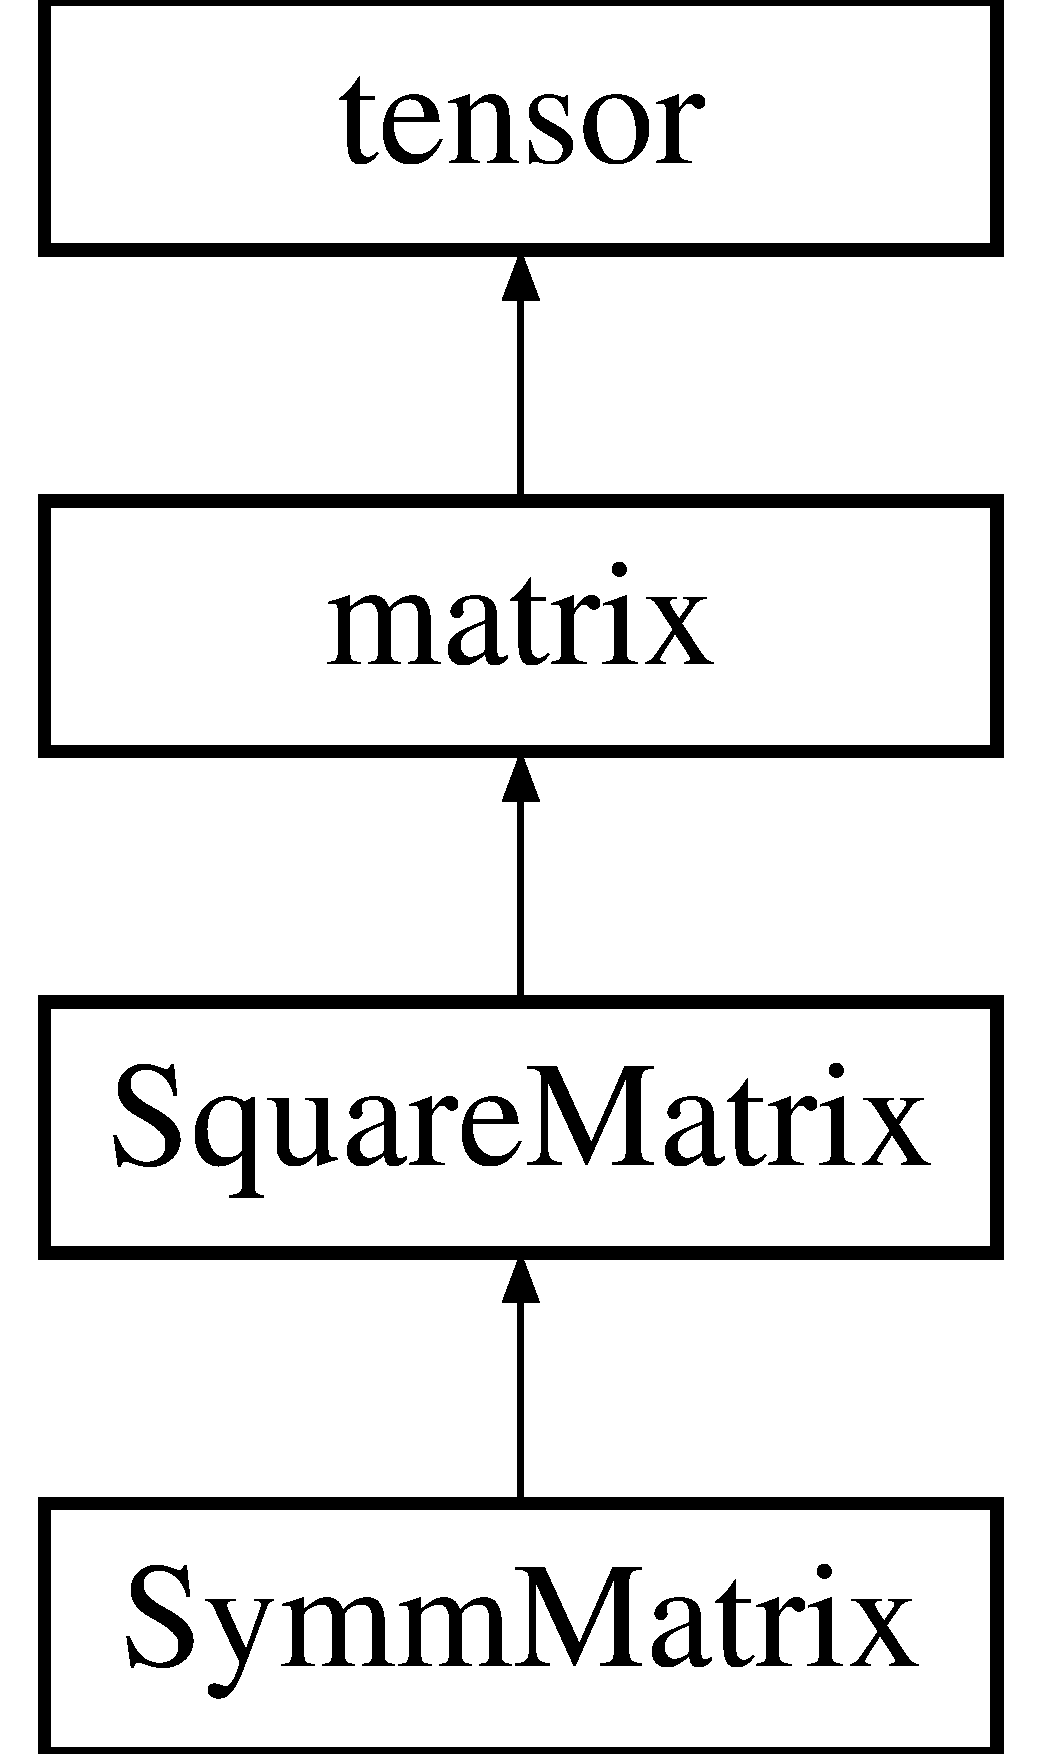
\includegraphics[height=4cm]{classJKBuilder_1_1SquareMatrix}
\end{center}
\end{figure}
\subsection*{Public Member Functions}
\begin{DoxyCompactItemize}
\item 
\hyperlink{classJKBuilder_1_1SquareMatrix_af755a00337cbb65c3456c2d2c80cdb08}{SquareMatrix} (const int n, const bool Init=false)
\begin{DoxyCompactList}\small\item\em Allocates memory for an n$\ast$n \hyperlink{classJKBuilder_1_1matrix}{matrix} and sets it to 0 if Init==true (default is false). \item\end{DoxyCompactList}\item 
\hyperlink{classJKBuilder_1_1SquareMatrix_a9b4d71581dc48d35a53e3e63a86be2b0}{SquareMatrix} (const double $\ast$DaMatrix, const int n)
\begin{DoxyCompactList}\small\item\em Makes an n by n \hyperlink{classJKBuilder_1_1matrix}{matrix} by copying DaMatrix. \item\end{DoxyCompactList}\item 
\hyperlink{classJKBuilder_1_1SquareMatrix_adfb34b7570c1de2cf7b96ba76fde9b01}{SquareMatrix} (double $\ast$DaMatrix, const int n)
\begin{DoxyCompactList}\small\item\em Sets this \hyperlink{classJKBuilder_1_1matrix}{matrix} equal to the n by m \hyperlink{classJKBuilder_1_1matrix}{matrix} DaMatrix. \item\end{DoxyCompactList}\item 
\hyperlink{classJKBuilder_1_1SquareMatrix_a2ef83e63ad627a33ea913bc245f00f43}{SquareMatrix} (const \hyperlink{classJKBuilder_1_1SquareMatrix}{SquareMatrix} \&other)
\begin{DoxyCompactList}\small\item\em Makes this \hyperlink{classJKBuilder_1_1matrix}{matrix} a copy of other. \item\end{DoxyCompactList}\item 
\hyperlink{classJKBuilder_1_1SquareMatrix}{SquareMatrix} \& \hyperlink{classJKBuilder_1_1SquareMatrix_ad78e5a12d26f1984d77a57095bc4d181}{operator=} (const \hyperlink{classJKBuilder_1_1SquareMatrix}{SquareMatrix} \&other)
\begin{DoxyCompactList}\small\item\em Sets this \hyperlink{classJKBuilder_1_1matrix}{matrix} equal to the other one. \item\end{DoxyCompactList}\item 
void \hyperlink{classJKBuilder_1_1matrix_af2563817f6505e9f8a6ee5c5c209a115}{T} ()
\begin{DoxyCompactList}\small\item\em Transposes a \hyperlink{classJKBuilder_1_1matrix}{matrix} by flipping the flag (don't forget to un-\/transpose it). \item\end{DoxyCompactList}\item 
const double \& \hyperlink{classJKBuilder_1_1matrix_a9ccbac42f4eefb704f04886001f4fb3e}{operator()} (const int i, const int j) const 
\begin{DoxyCompactList}\small\item\em Returns a non-\/editable element (i,j). \item\end{DoxyCompactList}\item 
double \& \hyperlink{classJKBuilder_1_1matrix_a3d7fca183ff1c9f4c160218746f2ef31}{operator()} (const int i, const int j)
\begin{DoxyCompactList}\small\item\em Returns an editable element (i,j). \item\end{DoxyCompactList}\item 
\hyperlink{classJKBuilder_1_1matrix}{matrix} \& \hyperlink{classJKBuilder_1_1matrix_ad4799cbe4a5d07c77f41857a3ce914a2}{operator$\ast$} (const double alpha)
\begin{DoxyCompactList}\small\item\em Scales a \hyperlink{classJKBuilder_1_1matrix}{matrix} by alpha. \item\end{DoxyCompactList}\item 
void \hyperlink{classJKBuilder_1_1tensor_a0ca5cbe96d2a61f06ae4b543ef84f166}{Alloc} ()
\item 
bool \hyperlink{classJKBuilder_1_1tensor_a79c9a36acc5dbeab94033ca97971dc09}{IsSet} () const 
\begin{DoxyCompactList}\small\item\em Returns true if this \hyperlink{classJKBuilder_1_1tensor}{tensor} is allocated and DimsGood==true (roughly the equiv to asking if this is NULL). \item\end{DoxyCompactList}\item 
virtual void \hyperlink{classJKBuilder_1_1tensor_a98b1050f09da390896f964fb7a892391}{Initialize} ()
\begin{DoxyCompactList}\small\item\em Sets all elements to zero in the \hyperlink{classJKBuilder_1_1tensor}{tensor}, which obviously overwrites the contents. \item\end{DoxyCompactList}\item 
virtual void \hyperlink{classJKBuilder_1_1tensor_a10ffea2bf428adfa3e8319646c44a3c6}{Update} (const double $\ast$Tensor)
\begin{DoxyCompactList}\small\item\em Updates DaTensor so that it is the same as Tensor. \item\end{DoxyCompactList}\item 
int \hyperlink{classJKBuilder_1_1tensor_a537b2f14296e2f0e62f00e1703c5fa08}{TotalElements} ()
\item 
int \hyperlink{classJKBuilder_1_1tensor_a6bdcfca6493bc217b607317dbceb28b2}{DimI} (const int i) const 
\begin{DoxyCompactList}\small\item\em Returns dimension i (counting from 0). \item\end{DoxyCompactList}\item 
void \hyperlink{classJKBuilder_1_1tensor_ace6bcf62c74395ab9e37abc4935f66e0}{SetDimensions} (const int $\ast$DesiredDimensions)
\begin{DoxyCompactList}\small\item\em Copies the dimensions you want (DesiredDimensions), into the \hyperlink{classJKBuilder_1_1tensor_a2ce1e6e0782ddee097f2c4aa2663d3e9}{tensor::dimensions}. Overwrites the contents. \item\end{DoxyCompactList}\item 
virtual void \hyperlink{classJKBuilder_1_1tensor_a388f572c62279f839ee138a9afbdeeb5}{print} ()
\begin{DoxyCompactList}\small\item\em Debugging function that prints the \hyperlink{classJKBuilder_1_1tensor}{tensor} (current model not appropriate for a distributed \hyperlink{classJKBuilder_1_1tensor}{tensor}) to the \hyperlink{classJKBuilder_1_1printer}{printer}. \item\end{DoxyCompactList}\item 
virtual void \hyperlink{classJKBuilder_1_1tensor_a74b2fe351a5444c1325870dc6162f451}{print} (\hyperlink{classJKBuilder_1_1IOManager}{IOManager} \&output)
\begin{DoxyCompactList}\small\item\em Allows the user to select the destination of the printed \hyperlink{classJKBuilder_1_1tensor}{tensor}. \item\end{DoxyCompactList}\item 
const double \& \hyperlink{classJKBuilder_1_1tensor_a4f0dc1b84b580cec49500c70f87e084a}{operator\mbox{[}$\,$\mbox{]}} (const int i) const 
\begin{DoxyCompactList}\small\item\em Returns a non-\/modifiable element i of the \hyperlink{classJKBuilder_1_1tensor}{tensor}. \item\end{DoxyCompactList}\item 
double \& \hyperlink{classJKBuilder_1_1tensor_a38c9fed6b117f7cf8b76785648d76b62}{operator\mbox{[}$\,$\mbox{]}} (const int i)
\begin{DoxyCompactList}\small\item\em Returns a modifiable element i of the \hyperlink{classJKBuilder_1_1tensor}{tensor}. \item\end{DoxyCompactList}\item 
bool \hyperlink{classJKBuilder_1_1tensor_a10ae0b61e655854d12c6465d2b9e3506}{operator==} (const \hyperlink{classJKBuilder_1_1tensor}{tensor} \&other)
\begin{DoxyCompactList}\small\item\em Returns true iff this \hyperlink{classJKBuilder_1_1tensor}{tensor} is equal to the other one. \item\end{DoxyCompactList}\item 
bool \hyperlink{classJKBuilder_1_1tensor_a9b42dd835ddf2eb1a26b5d525b59b2b8}{operator!=} (const \hyperlink{classJKBuilder_1_1tensor}{tensor} \&other)
\begin{DoxyCompactList}\small\item\em Returns the opposite of operator==. \item\end{DoxyCompactList}\item 
const double $\ast$ \hyperlink{classJKBuilder_1_1tensor_a6a4e024f566d3bf9ba32a349afc5bbcf}{Address} () const 
\begin{DoxyCompactList}\small\item\em Returns the starting address of the actual data so that pointers can just be passed. \item\end{DoxyCompactList}\item 
double $\ast$ \hyperlink{classJKBuilder_1_1tensor_ac982d9eb84092bfc13694448dd824cbc}{Address} ()
\end{DoxyCompactItemize}
\subsection*{Protected Member Functions}
\begin{DoxyCompactItemize}
\item 
bool \hyperlink{classJKBuilder_1_1tensor_a6e72344440b411f433eb50171648c2d0}{DimsGood} () const 
\begin{DoxyCompactList}\small\item\em Returns true if the dimensions appear set (dimensions!=NULL \&\& dimensions\mbox{[}i\mbox{]}$>$0 for all i). \item\end{DoxyCompactList}\end{DoxyCompactItemize}
\subsection*{Protected Attributes}
\begin{DoxyCompactItemize}
\item 
bool \hyperlink{classJKBuilder_1_1matrix_a77fa48e57c519482de2ec7ec182b16ef}{IsTransposed}
\begin{DoxyCompactList}\small\item\em A flag that tells us if our \hyperlink{classJKBuilder_1_1matrix}{matrix} is transposed. \item\end{DoxyCompactList}\item 
int \hyperlink{classJKBuilder_1_1tensor_a6cfd95afd0afebd625b889fb6e58371c}{rank}
\begin{DoxyCompactList}\small\item\em This is the rank of the \hyperlink{classJKBuilder_1_1tensor}{tensor}. \item\end{DoxyCompactList}\item 
double $\ast$ \hyperlink{classJKBuilder_1_1tensor_a91f7b1e58c0e5d1a49ddb8b80ab7790e}{DaTensor}
\begin{DoxyCompactList}\small\item\em Realistically we are going to want to use this for doubles, so I am not declaring this a template. \item\end{DoxyCompactList}\item 
int \hyperlink{classJKBuilder_1_1tensor_a23ae6a00bed19d2ad34d439636e797da}{nelements}
\begin{DoxyCompactList}\small\item\em This is the total number of elements in the \hyperlink{classJKBuilder_1_1tensor}{tensor}. \item\end{DoxyCompactList}\item 
int $\ast$ \hyperlink{classJKBuilder_1_1tensor_a2ce1e6e0782ddee097f2c4aa2663d3e9}{dimensions}
\begin{DoxyCompactList}\small\item\em This is the array of \hyperlink{classJKBuilder_1_1tensor}{tensor} dimensions (row,column). \item\end{DoxyCompactList}\end{DoxyCompactItemize}


\subsection{Detailed Description}
A generalization of the \hyperlink{classJKBuilder_1_1matrix}{matrix} class to square matrices. The main difference, to the user, is that square matrices do not require two indices. 

\subsection{Constructor \& Destructor Documentation}
\hypertarget{classJKBuilder_1_1SquareMatrix_af755a00337cbb65c3456c2d2c80cdb08}{
\index{JKBuilder::SquareMatrix@{JKBuilder::SquareMatrix}!SquareMatrix@{SquareMatrix}}
\index{SquareMatrix@{SquareMatrix}!JKBuilder::SquareMatrix@{JKBuilder::SquareMatrix}}
\subsubsection[{SquareMatrix}]{\setlength{\rightskip}{0pt plus 5cm}{\bf SquareMatrix} (const int {\em n}, \/  const bool {\em Init} = {\ttfamily false})}}
\label{classJKBuilder_1_1SquareMatrix_af755a00337cbb65c3456c2d2c80cdb08}


Allocates memory for an n$\ast$n \hyperlink{classJKBuilder_1_1matrix}{matrix} and sets it to 0 if Init==true (default is false). \hypertarget{classJKBuilder_1_1SquareMatrix_a9b4d71581dc48d35a53e3e63a86be2b0}{
\index{JKBuilder::SquareMatrix@{JKBuilder::SquareMatrix}!SquareMatrix@{SquareMatrix}}
\index{SquareMatrix@{SquareMatrix}!JKBuilder::SquareMatrix@{JKBuilder::SquareMatrix}}
\subsubsection[{SquareMatrix}]{\setlength{\rightskip}{0pt plus 5cm}{\bf SquareMatrix} (const double $\ast$ {\em DaMatrix}, \/  const int {\em n})}}
\label{classJKBuilder_1_1SquareMatrix_a9b4d71581dc48d35a53e3e63a86be2b0}


Makes an n by n \hyperlink{classJKBuilder_1_1matrix}{matrix} by copying DaMatrix. \hypertarget{classJKBuilder_1_1SquareMatrix_adfb34b7570c1de2cf7b96ba76fde9b01}{
\index{JKBuilder::SquareMatrix@{JKBuilder::SquareMatrix}!SquareMatrix@{SquareMatrix}}
\index{SquareMatrix@{SquareMatrix}!JKBuilder::SquareMatrix@{JKBuilder::SquareMatrix}}
\subsubsection[{SquareMatrix}]{\setlength{\rightskip}{0pt plus 5cm}{\bf SquareMatrix} (double $\ast$ {\em DaMatrix}, \/  const int {\em n})}}
\label{classJKBuilder_1_1SquareMatrix_adfb34b7570c1de2cf7b96ba76fde9b01}


Sets this \hyperlink{classJKBuilder_1_1matrix}{matrix} equal to the n by m \hyperlink{classJKBuilder_1_1matrix}{matrix} DaMatrix. \hypertarget{classJKBuilder_1_1SquareMatrix_a2ef83e63ad627a33ea913bc245f00f43}{
\index{JKBuilder::SquareMatrix@{JKBuilder::SquareMatrix}!SquareMatrix@{SquareMatrix}}
\index{SquareMatrix@{SquareMatrix}!JKBuilder::SquareMatrix@{JKBuilder::SquareMatrix}}
\subsubsection[{SquareMatrix}]{\setlength{\rightskip}{0pt plus 5cm}{\bf SquareMatrix} (const {\bf SquareMatrix} \& {\em other})}}
\label{classJKBuilder_1_1SquareMatrix_a2ef83e63ad627a33ea913bc245f00f43}


Makes this \hyperlink{classJKBuilder_1_1matrix}{matrix} a copy of other. 

\subsection{Member Function Documentation}
\hypertarget{classJKBuilder_1_1SquareMatrix_ad78e5a12d26f1984d77a57095bc4d181}{
\index{JKBuilder::SquareMatrix@{JKBuilder::SquareMatrix}!operator=@{operator=}}
\index{operator=@{operator=}!JKBuilder::SquareMatrix@{JKBuilder::SquareMatrix}}
\subsubsection[{operator=}]{\setlength{\rightskip}{0pt plus 5cm}{\bf SquareMatrix} \& operator= (const {\bf SquareMatrix} \& {\em other})}}
\label{classJKBuilder_1_1SquareMatrix_ad78e5a12d26f1984d77a57095bc4d181}


Sets this \hyperlink{classJKBuilder_1_1matrix}{matrix} equal to the other one. 

Reimplemented from \hyperlink{classJKBuilder_1_1matrix_a11df53cc3fc568369a9f612cfb556680}{matrix}.

Reimplemented in \hyperlink{classJKBuilder_1_1SymmMatrix_aca4a8297278ff39c5422febf1dcbc5ac}{SymmMatrix}.\hypertarget{classJKBuilder_1_1matrix_af2563817f6505e9f8a6ee5c5c209a115}{
\index{JKBuilder::SquareMatrix@{JKBuilder::SquareMatrix}!T@{T}}
\index{T@{T}!JKBuilder::SquareMatrix@{JKBuilder::SquareMatrix}}
\subsubsection[{T}]{\setlength{\rightskip}{0pt plus 5cm}void T ()\hspace{0.3cm}{\ttfamily  \mbox{[}inherited\mbox{]}}}}
\label{classJKBuilder_1_1matrix_af2563817f6505e9f8a6ee5c5c209a115}


Transposes a \hyperlink{classJKBuilder_1_1matrix}{matrix} by flipping the flag (don't forget to un-\/transpose it). \hypertarget{classJKBuilder_1_1matrix_a9ccbac42f4eefb704f04886001f4fb3e}{
\index{JKBuilder::SquareMatrix@{JKBuilder::SquareMatrix}!operator()@{operator()}}
\index{operator()@{operator()}!JKBuilder::SquareMatrix@{JKBuilder::SquareMatrix}}
\subsubsection[{operator()}]{\setlength{\rightskip}{0pt plus 5cm}const double \& operator() (const int {\em i}, \/  const int {\em j}) const\hspace{0.3cm}{\ttfamily  \mbox{[}inherited\mbox{]}}}}
\label{classJKBuilder_1_1matrix_a9ccbac42f4eefb704f04886001f4fb3e}


Returns a non-\/editable element (i,j). 

Reimplemented in \hyperlink{classJKBuilder_1_1SymmMatrix_a9ccbac42f4eefb704f04886001f4fb3e}{SymmMatrix}.\hypertarget{classJKBuilder_1_1matrix_a3d7fca183ff1c9f4c160218746f2ef31}{
\index{JKBuilder::SquareMatrix@{JKBuilder::SquareMatrix}!operator()@{operator()}}
\index{operator()@{operator()}!JKBuilder::SquareMatrix@{JKBuilder::SquareMatrix}}
\subsubsection[{operator()}]{\setlength{\rightskip}{0pt plus 5cm}double \& operator() (const int {\em i}, \/  const int {\em j})\hspace{0.3cm}{\ttfamily  \mbox{[}inherited\mbox{]}}}}
\label{classJKBuilder_1_1matrix_a3d7fca183ff1c9f4c160218746f2ef31}


Returns an editable element (i,j). 

Reimplemented in \hyperlink{classJKBuilder_1_1SymmMatrix_a3d7fca183ff1c9f4c160218746f2ef31}{SymmMatrix}.\hypertarget{classJKBuilder_1_1matrix_ad4799cbe4a5d07c77f41857a3ce914a2}{
\index{JKBuilder::SquareMatrix@{JKBuilder::SquareMatrix}!operator$\ast$@{operator$\ast$}}
\index{operator$\ast$@{operator$\ast$}!JKBuilder::SquareMatrix@{JKBuilder::SquareMatrix}}
\subsubsection[{operator$\ast$}]{\setlength{\rightskip}{0pt plus 5cm}{\bf matrix} \& operator$\ast$ (const double {\em alpha})\hspace{0.3cm}{\ttfamily  \mbox{[}inherited\mbox{]}}}}
\label{classJKBuilder_1_1matrix_ad4799cbe4a5d07c77f41857a3ce914a2}


Scales a \hyperlink{classJKBuilder_1_1matrix}{matrix} by alpha. \hypertarget{classJKBuilder_1_1tensor_a6e72344440b411f433eb50171648c2d0}{
\index{JKBuilder::SquareMatrix@{JKBuilder::SquareMatrix}!DimsGood@{DimsGood}}
\index{DimsGood@{DimsGood}!JKBuilder::SquareMatrix@{JKBuilder::SquareMatrix}}
\subsubsection[{DimsGood}]{\setlength{\rightskip}{0pt plus 5cm}bool DimsGood () const\hspace{0.3cm}{\ttfamily  \mbox{[}protected, inherited\mbox{]}}}}
\label{classJKBuilder_1_1tensor_a6e72344440b411f433eb50171648c2d0}


Returns true if the dimensions appear set (dimensions!=NULL \&\& dimensions\mbox{[}i\mbox{]}$>$0 for all i). \hypertarget{classJKBuilder_1_1tensor_a0ca5cbe96d2a61f06ae4b543ef84f166}{
\index{JKBuilder::SquareMatrix@{JKBuilder::SquareMatrix}!Alloc@{Alloc}}
\index{Alloc@{Alloc}!JKBuilder::SquareMatrix@{JKBuilder::SquareMatrix}}
\subsubsection[{Alloc}]{\setlength{\rightskip}{0pt plus 5cm}void Alloc ()\hspace{0.3cm}{\ttfamily  \mbox{[}inherited\mbox{]}}}}
\label{classJKBuilder_1_1tensor_a0ca5cbe96d2a61f06ae4b543ef84f166}
The following function can never be virtual because base operations of the Tensor depend on them The actual memory allocation call, if DaTensor==NULL allocates the memory \hypertarget{classJKBuilder_1_1tensor_a79c9a36acc5dbeab94033ca97971dc09}{
\index{JKBuilder::SquareMatrix@{JKBuilder::SquareMatrix}!IsSet@{IsSet}}
\index{IsSet@{IsSet}!JKBuilder::SquareMatrix@{JKBuilder::SquareMatrix}}
\subsubsection[{IsSet}]{\setlength{\rightskip}{0pt plus 5cm}bool IsSet () const\hspace{0.3cm}{\ttfamily  \mbox{[}inherited\mbox{]}}}}
\label{classJKBuilder_1_1tensor_a79c9a36acc5dbeab94033ca97971dc09}


Returns true if this \hyperlink{classJKBuilder_1_1tensor}{tensor} is allocated and DimsGood==true (roughly the equiv to asking if this is NULL). \hypertarget{classJKBuilder_1_1tensor_a98b1050f09da390896f964fb7a892391}{
\index{JKBuilder::SquareMatrix@{JKBuilder::SquareMatrix}!Initialize@{Initialize}}
\index{Initialize@{Initialize}!JKBuilder::SquareMatrix@{JKBuilder::SquareMatrix}}
\subsubsection[{Initialize}]{\setlength{\rightskip}{0pt plus 5cm}void Initialize ()\hspace{0.3cm}{\ttfamily  \mbox{[}virtual, inherited\mbox{]}}}}
\label{classJKBuilder_1_1tensor_a98b1050f09da390896f964fb7a892391}


Sets all elements to zero in the \hyperlink{classJKBuilder_1_1tensor}{tensor}, which obviously overwrites the contents. 

Reimplemented in \hyperlink{classJKBuilder_1_1DistributedMatrix_a98b1050f09da390896f964fb7a892391}{DistributedMatrix}.\hypertarget{classJKBuilder_1_1tensor_a10ffea2bf428adfa3e8319646c44a3c6}{
\index{JKBuilder::SquareMatrix@{JKBuilder::SquareMatrix}!Update@{Update}}
\index{Update@{Update}!JKBuilder::SquareMatrix@{JKBuilder::SquareMatrix}}
\subsubsection[{Update}]{\setlength{\rightskip}{0pt plus 5cm}void Update (const double $\ast$ {\em Tensor})\hspace{0.3cm}{\ttfamily  \mbox{[}virtual, inherited\mbox{]}}}}
\label{classJKBuilder_1_1tensor_a10ffea2bf428adfa3e8319646c44a3c6}


Updates DaTensor so that it is the same as Tensor. Update always takes the full Tensor, not a block of it. It is child class's jobs to scatter the data if need be. 

Reimplemented in \hyperlink{classJKBuilder_1_1DistributedMatrix_a6a378face23ba83b2431cb08e8519066}{DistributedMatrix}.\hypertarget{classJKBuilder_1_1tensor_a537b2f14296e2f0e62f00e1703c5fa08}{
\index{JKBuilder::SquareMatrix@{JKBuilder::SquareMatrix}!TotalElements@{TotalElements}}
\index{TotalElements@{TotalElements}!JKBuilder::SquareMatrix@{JKBuilder::SquareMatrix}}
\subsubsection[{TotalElements}]{\setlength{\rightskip}{0pt plus 5cm}int TotalElements ()\hspace{0.3cm}{\ttfamily  \mbox{[}inherited\mbox{]}}}}
\label{classJKBuilder_1_1tensor_a537b2f14296e2f0e62f00e1703c5fa08}
\hypertarget{classJKBuilder_1_1tensor_a6bdcfca6493bc217b607317dbceb28b2}{
\index{JKBuilder::SquareMatrix@{JKBuilder::SquareMatrix}!DimI@{DimI}}
\index{DimI@{DimI}!JKBuilder::SquareMatrix@{JKBuilder::SquareMatrix}}
\subsubsection[{DimI}]{\setlength{\rightskip}{0pt plus 5cm}int DimI (const int {\em i}) const\hspace{0.3cm}{\ttfamily  \mbox{[}inherited\mbox{]}}}}
\label{classJKBuilder_1_1tensor_a6bdcfca6493bc217b607317dbceb28b2}


Returns dimension i (counting from 0). \hypertarget{classJKBuilder_1_1tensor_ace6bcf62c74395ab9e37abc4935f66e0}{
\index{JKBuilder::SquareMatrix@{JKBuilder::SquareMatrix}!SetDimensions@{SetDimensions}}
\index{SetDimensions@{SetDimensions}!JKBuilder::SquareMatrix@{JKBuilder::SquareMatrix}}
\subsubsection[{SetDimensions}]{\setlength{\rightskip}{0pt plus 5cm}void SetDimensions (const int $\ast$ {\em DesiredDimensions})\hspace{0.3cm}{\ttfamily  \mbox{[}inherited\mbox{]}}}}
\label{classJKBuilder_1_1tensor_ace6bcf62c74395ab9e37abc4935f66e0}


Copies the dimensions you want (DesiredDimensions), into the \hyperlink{classJKBuilder_1_1tensor_a2ce1e6e0782ddee097f2c4aa2663d3e9}{tensor::dimensions}. Overwrites the contents. \hypertarget{classJKBuilder_1_1tensor_a388f572c62279f839ee138a9afbdeeb5}{
\index{JKBuilder::SquareMatrix@{JKBuilder::SquareMatrix}!print@{print}}
\index{print@{print}!JKBuilder::SquareMatrix@{JKBuilder::SquareMatrix}}
\subsubsection[{print}]{\setlength{\rightskip}{0pt plus 5cm}void print ()\hspace{0.3cm}{\ttfamily  \mbox{[}virtual, inherited\mbox{]}}}}
\label{classJKBuilder_1_1tensor_a388f572c62279f839ee138a9afbdeeb5}


Debugging function that prints the \hyperlink{classJKBuilder_1_1tensor}{tensor} (current model not appropriate for a distributed \hyperlink{classJKBuilder_1_1tensor}{tensor}) to the \hyperlink{classJKBuilder_1_1printer}{printer}. 

Reimplemented in \hyperlink{classJKBuilder_1_1DistributedMatrix_a388f572c62279f839ee138a9afbdeeb5}{DistributedMatrix}.\hypertarget{classJKBuilder_1_1tensor_a74b2fe351a5444c1325870dc6162f451}{
\index{JKBuilder::SquareMatrix@{JKBuilder::SquareMatrix}!print@{print}}
\index{print@{print}!JKBuilder::SquareMatrix@{JKBuilder::SquareMatrix}}
\subsubsection[{print}]{\setlength{\rightskip}{0pt plus 5cm}void print ({\bf IOManager} \& {\em output})\hspace{0.3cm}{\ttfamily  \mbox{[}virtual, inherited\mbox{]}}}}
\label{classJKBuilder_1_1tensor_a74b2fe351a5444c1325870dc6162f451}


Allows the user to select the destination of the printed \hyperlink{classJKBuilder_1_1tensor}{tensor}. 

Reimplemented in \hyperlink{classJKBuilder_1_1DistributedMatrix_a74b2fe351a5444c1325870dc6162f451}{DistributedMatrix}.\hypertarget{classJKBuilder_1_1tensor_a4f0dc1b84b580cec49500c70f87e084a}{
\index{JKBuilder::SquareMatrix@{JKBuilder::SquareMatrix}!operator\mbox{[}\mbox{]}@{operator[]}}
\index{operator\mbox{[}\mbox{]}@{operator[]}!JKBuilder::SquareMatrix@{JKBuilder::SquareMatrix}}
\subsubsection[{operator[]}]{\setlength{\rightskip}{0pt plus 5cm}const double \& operator\mbox{[}$\,$\mbox{]} (const int {\em i}) const\hspace{0.3cm}{\ttfamily  \mbox{[}inherited\mbox{]}}}}
\label{classJKBuilder_1_1tensor_a4f0dc1b84b580cec49500c70f87e084a}


Returns a non-\/modifiable element i of the \hyperlink{classJKBuilder_1_1tensor}{tensor}. \hypertarget{classJKBuilder_1_1tensor_a38c9fed6b117f7cf8b76785648d76b62}{
\index{JKBuilder::SquareMatrix@{JKBuilder::SquareMatrix}!operator\mbox{[}\mbox{]}@{operator[]}}
\index{operator\mbox{[}\mbox{]}@{operator[]}!JKBuilder::SquareMatrix@{JKBuilder::SquareMatrix}}
\subsubsection[{operator[]}]{\setlength{\rightskip}{0pt plus 5cm}double \& operator\mbox{[}$\,$\mbox{]} (const int {\em i})\hspace{0.3cm}{\ttfamily  \mbox{[}inherited\mbox{]}}}}
\label{classJKBuilder_1_1tensor_a38c9fed6b117f7cf8b76785648d76b62}


Returns a modifiable element i of the \hyperlink{classJKBuilder_1_1tensor}{tensor}. \hypertarget{classJKBuilder_1_1tensor_a10ae0b61e655854d12c6465d2b9e3506}{
\index{JKBuilder::SquareMatrix@{JKBuilder::SquareMatrix}!operator==@{operator==}}
\index{operator==@{operator==}!JKBuilder::SquareMatrix@{JKBuilder::SquareMatrix}}
\subsubsection[{operator==}]{\setlength{\rightskip}{0pt plus 5cm}bool operator== (const {\bf tensor} \& {\em other})\hspace{0.3cm}{\ttfamily  \mbox{[}inherited\mbox{]}}}}
\label{classJKBuilder_1_1tensor_a10ae0b61e655854d12c6465d2b9e3506}


Returns true iff this \hyperlink{classJKBuilder_1_1tensor}{tensor} is equal to the other one. \hypertarget{classJKBuilder_1_1tensor_a9b42dd835ddf2eb1a26b5d525b59b2b8}{
\index{JKBuilder::SquareMatrix@{JKBuilder::SquareMatrix}!operator!=@{operator!=}}
\index{operator!=@{operator!=}!JKBuilder::SquareMatrix@{JKBuilder::SquareMatrix}}
\subsubsection[{operator!=}]{\setlength{\rightskip}{0pt plus 5cm}bool operator!= (const {\bf tensor} \& {\em other})\hspace{0.3cm}{\ttfamily  \mbox{[}inherited\mbox{]}}}}
\label{classJKBuilder_1_1tensor_a9b42dd835ddf2eb1a26b5d525b59b2b8}


Returns the opposite of operator==. \hypertarget{classJKBuilder_1_1tensor_a6a4e024f566d3bf9ba32a349afc5bbcf}{
\index{JKBuilder::SquareMatrix@{JKBuilder::SquareMatrix}!Address@{Address}}
\index{Address@{Address}!JKBuilder::SquareMatrix@{JKBuilder::SquareMatrix}}
\subsubsection[{Address}]{\setlength{\rightskip}{0pt plus 5cm}const double $\ast$ Address () const\hspace{0.3cm}{\ttfamily  \mbox{[}inherited\mbox{]}}}}
\label{classJKBuilder_1_1tensor_a6a4e024f566d3bf9ba32a349afc5bbcf}


Returns the starting address of the actual data so that pointers can just be passed. \hypertarget{classJKBuilder_1_1tensor_ac982d9eb84092bfc13694448dd824cbc}{
\index{JKBuilder::SquareMatrix@{JKBuilder::SquareMatrix}!Address@{Address}}
\index{Address@{Address}!JKBuilder::SquareMatrix@{JKBuilder::SquareMatrix}}
\subsubsection[{Address}]{\setlength{\rightskip}{0pt plus 5cm}double $\ast$ Address ()\hspace{0.3cm}{\ttfamily  \mbox{[}inherited\mbox{]}}}}
\label{classJKBuilder_1_1tensor_ac982d9eb84092bfc13694448dd824cbc}


\subsection{Member Data Documentation}
\hypertarget{classJKBuilder_1_1matrix_a77fa48e57c519482de2ec7ec182b16ef}{
\index{JKBuilder::SquareMatrix@{JKBuilder::SquareMatrix}!IsTransposed@{IsTransposed}}
\index{IsTransposed@{IsTransposed}!JKBuilder::SquareMatrix@{JKBuilder::SquareMatrix}}
\subsubsection[{IsTransposed}]{\setlength{\rightskip}{0pt plus 5cm}bool {\bf IsTransposed}\hspace{0.3cm}{\ttfamily  \mbox{[}protected, inherited\mbox{]}}}}
\label{classJKBuilder_1_1matrix_a77fa48e57c519482de2ec7ec182b16ef}


A flag that tells us if our \hyperlink{classJKBuilder_1_1matrix}{matrix} is transposed. \hypertarget{classJKBuilder_1_1tensor_a6cfd95afd0afebd625b889fb6e58371c}{
\index{JKBuilder::SquareMatrix@{JKBuilder::SquareMatrix}!rank@{rank}}
\index{rank@{rank}!JKBuilder::SquareMatrix@{JKBuilder::SquareMatrix}}
\subsubsection[{rank}]{\setlength{\rightskip}{0pt plus 5cm}int {\bf rank}\hspace{0.3cm}{\ttfamily  \mbox{[}protected, inherited\mbox{]}}}}
\label{classJKBuilder_1_1tensor_a6cfd95afd0afebd625b889fb6e58371c}


This is the rank of the \hyperlink{classJKBuilder_1_1tensor}{tensor}. \hypertarget{classJKBuilder_1_1tensor_a91f7b1e58c0e5d1a49ddb8b80ab7790e}{
\index{JKBuilder::SquareMatrix@{JKBuilder::SquareMatrix}!DaTensor@{DaTensor}}
\index{DaTensor@{DaTensor}!JKBuilder::SquareMatrix@{JKBuilder::SquareMatrix}}
\subsubsection[{DaTensor}]{\setlength{\rightskip}{0pt plus 5cm}double$\ast$ {\bf DaTensor}\hspace{0.3cm}{\ttfamily  \mbox{[}protected, inherited\mbox{]}}}}
\label{classJKBuilder_1_1tensor_a91f7b1e58c0e5d1a49ddb8b80ab7790e}


Realistically we are going to want to use this for doubles, so I am not declaring this a template. \hypertarget{classJKBuilder_1_1tensor_a23ae6a00bed19d2ad34d439636e797da}{
\index{JKBuilder::SquareMatrix@{JKBuilder::SquareMatrix}!nelements@{nelements}}
\index{nelements@{nelements}!JKBuilder::SquareMatrix@{JKBuilder::SquareMatrix}}
\subsubsection[{nelements}]{\setlength{\rightskip}{0pt plus 5cm}int {\bf nelements}\hspace{0.3cm}{\ttfamily  \mbox{[}protected, inherited\mbox{]}}}}
\label{classJKBuilder_1_1tensor_a23ae6a00bed19d2ad34d439636e797da}


This is the total number of elements in the \hyperlink{classJKBuilder_1_1tensor}{tensor}. \hypertarget{classJKBuilder_1_1tensor_a2ce1e6e0782ddee097f2c4aa2663d3e9}{
\index{JKBuilder::SquareMatrix@{JKBuilder::SquareMatrix}!dimensions@{dimensions}}
\index{dimensions@{dimensions}!JKBuilder::SquareMatrix@{JKBuilder::SquareMatrix}}
\subsubsection[{dimensions}]{\setlength{\rightskip}{0pt plus 5cm}int$\ast$ {\bf dimensions}\hspace{0.3cm}{\ttfamily  \mbox{[}protected, inherited\mbox{]}}}}
\label{classJKBuilder_1_1tensor_a2ce1e6e0782ddee097f2c4aa2663d3e9}


This is the array of \hyperlink{classJKBuilder_1_1tensor}{tensor} dimensions (row,column). These dimensions are for the whole object, not blocks of it or anything else like that. What this means is that for say a 12 by 12 \hyperlink{classJKBuilder_1_1matrix}{matrix} distributed in 6 by 6 blocks these values are 12, not 6. 

The documentation for this class was generated from the following files:\begin{DoxyCompactItemize}
\item 
src/\hyperlink{SymmMatrix_8h}{SymmMatrix.h}\item 
src/\hyperlink{SymmMatrix_8cpp}{SymmMatrix.cpp}\end{DoxyCompactItemize}

\hypertarget{classJKBuilder_1_1SymmMatItr}{
\section{SymmMatItr Class Reference}
\label{classJKBuilder_1_1SymmMatItr}\index{JKBuilder::SymmMatItr@{JKBuilder::SymmMatItr}}
}


{\ttfamily \#include $<$SymmMatrix.h$>$}Inheritance diagram for SymmMatItr::\begin{figure}[H]
\begin{center}
\leavevmode
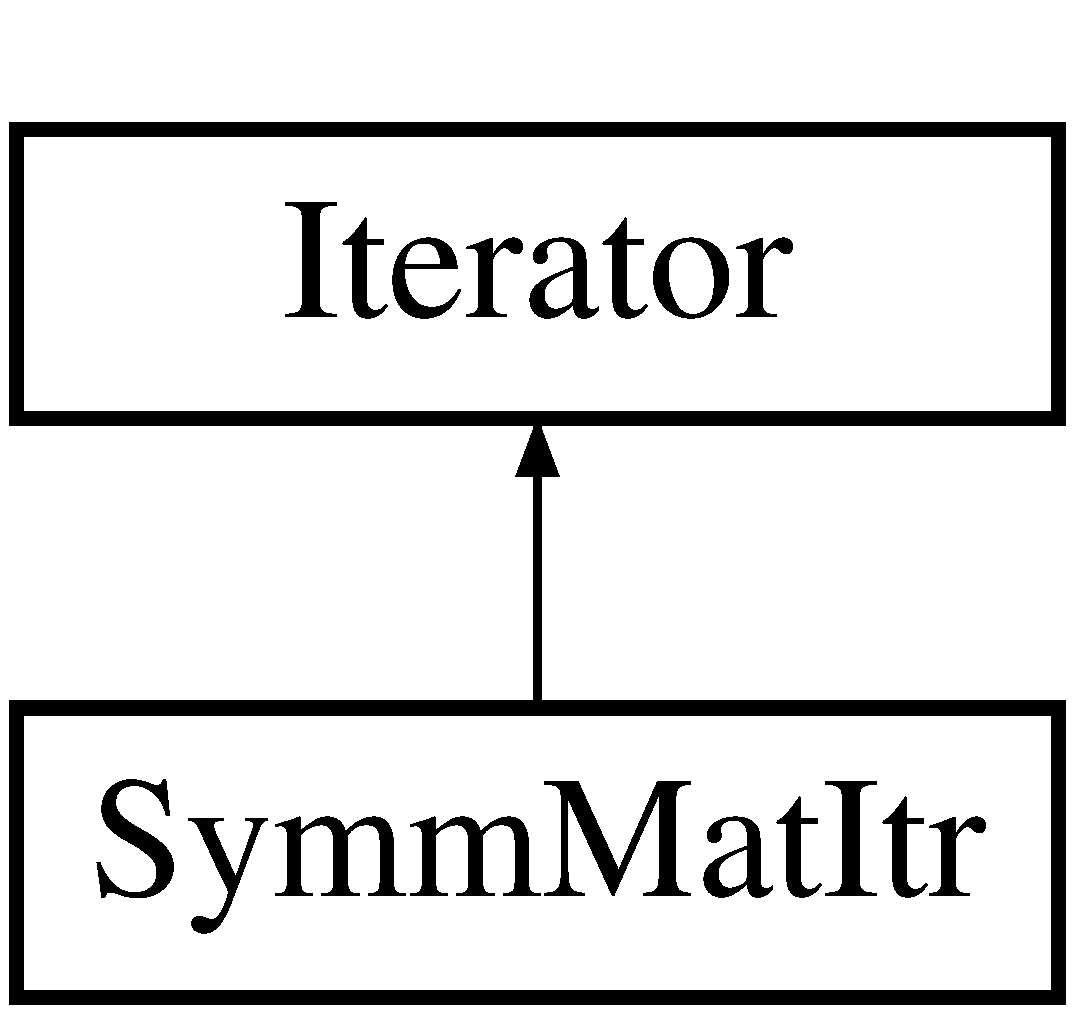
\includegraphics[height=2cm]{classJKBuilder_1_1SymmMatItr}
\end{center}
\end{figure}
\subsection*{Public Member Functions}
\begin{DoxyCompactItemize}
\item 
void \hyperlink{classJKBuilder_1_1SymmMatItr_a7874a07e98b52f4f147cde6f39353bae}{Iterate} ()
\begin{DoxyCompactList}\small\item\em The default NIndexIterator goes right to left, we want to go left to right and stop at diagonal. \item\end{DoxyCompactList}\item 
\hyperlink{classJKBuilder_1_1SymmMatItr_a5b2e8dde1f98a28e0e22b9fc4e911376}{SymmMatItr} (const int N, const bool end=false)
\item 
virtual void \hyperlink{classJKBuilder_1_1Iterator_a34ca36a99b20ae3170babadaffe51ed2}{Start} (int n=0)
\begin{DoxyCompactList}\small\item\em Returns an iterator suitable for starting on iteration n. \item\end{DoxyCompactList}\item 
virtual void \hyperlink{classJKBuilder_1_1Iterator_a5f692b73d2e160450f4617bb75825e11}{End} (int n=-\/1)
\begin{DoxyCompactList}\small\item\em Returns an iterator representing the state of the iterator after n iterations have occured. \item\end{DoxyCompactList}\item 
\hyperlink{classJKBuilder_1_1Iterator}{Iterator} \hyperlink{classJKBuilder_1_1Iterator_ac1702aedba13b4112b891b58dfd78eba}{operator++} (int)
\begin{DoxyCompactList}\small\item\em Increments the iterator after returning it's value. \item\end{DoxyCompactList}\item 
\hyperlink{classJKBuilder_1_1Iterator}{Iterator} \& \hyperlink{classJKBuilder_1_1Iterator_ae1f21c74128a5ef5d1b9de72ceb09be8}{operator++} ()
\begin{DoxyCompactList}\small\item\em Increments the iterator before returning it's value. \item\end{DoxyCompactList}\item 
bool \hyperlink{classJKBuilder_1_1Iterator_a1ea001976a5bc8ae8dc365e2a912b59a}{operator==} (const \hyperlink{classJKBuilder_1_1Iterator}{Iterator} \&other) const 
\item 
bool \hyperlink{classJKBuilder_1_1Iterator_a8c06af8ae0d9d1614ae9f81629275926}{operator!=} (const \hyperlink{classJKBuilder_1_1Iterator}{Iterator} \&other)
\begin{DoxyCompactList}\small\item\em Returns the opposite of operator==. \item\end{DoxyCompactList}\item 
void \hyperlink{classJKBuilder_1_1Iterator_aa83de505e29125c1d3ac7bb1b13ca15a}{SetStart} (std::vector$<$ int $>$ const \&other)
\begin{DoxyCompactList}\small\item\em Sets the N Indices to the N given in other. \item\end{DoxyCompactList}\item 
void \hyperlink{classJKBuilder_1_1Iterator_aad84ec668b5f41210db34c540aaa31fc}{SetEnd} (std::vector$<$ int $>$ const \&other)
\begin{DoxyCompactList}\small\item\em Sets the N MaxInd in other. \item\end{DoxyCompactList}\item 
int \hyperlink{classJKBuilder_1_1Iterator_a74247cf730a06b23fcb1ec64e5596b25}{operator\mbox{[}$\,$\mbox{]}} (const int i) const 
\begin{DoxyCompactList}\small\item\em Returns index i. \item\end{DoxyCompactList}\end{DoxyCompactItemize}
\subsection*{Protected Attributes}
\begin{DoxyCompactItemize}
\item 
std::vector$<$ int $>$ \hyperlink{classJKBuilder_1_1Iterator_a20ca24f6d827aba144bb087c4bcb74a0}{CurrentValue}
\begin{DoxyCompactList}\small\item\em The current value. \item\end{DoxyCompactList}\item 
std::vector$<$ int $>$ \hyperlink{classJKBuilder_1_1Iterator_ab6b56d3c4e9353bc938dd6249cde9ca0}{MaxInd}
\begin{DoxyCompactList}\small\item\em This is a vector of length N containing the maximum each index can be. \item\end{DoxyCompactList}\end{DoxyCompactItemize}


\subsection{Constructor \& Destructor Documentation}
\hypertarget{classJKBuilder_1_1SymmMatItr_a5b2e8dde1f98a28e0e22b9fc4e911376}{
\index{JKBuilder::SymmMatItr@{JKBuilder::SymmMatItr}!SymmMatItr@{SymmMatItr}}
\index{SymmMatItr@{SymmMatItr}!JKBuilder::SymmMatItr@{JKBuilder::SymmMatItr}}
\subsubsection[{SymmMatItr}]{\setlength{\rightskip}{0pt plus 5cm}{\bf SymmMatItr} (const int {\em N}, \/  const bool {\em end} = {\ttfamily false})}}
\label{classJKBuilder_1_1SymmMatItr_a5b2e8dde1f98a28e0e22b9fc4e911376}


\subsection{Member Function Documentation}
\hypertarget{classJKBuilder_1_1SymmMatItr_a7874a07e98b52f4f147cde6f39353bae}{
\index{JKBuilder::SymmMatItr@{JKBuilder::SymmMatItr}!Iterate@{Iterate}}
\index{Iterate@{Iterate}!JKBuilder::SymmMatItr@{JKBuilder::SymmMatItr}}
\subsubsection[{Iterate}]{\setlength{\rightskip}{0pt plus 5cm}void Iterate ()\hspace{0.3cm}{\ttfamily  \mbox{[}virtual\mbox{]}}}}
\label{classJKBuilder_1_1SymmMatItr_a7874a07e98b52f4f147cde6f39353bae}


The default NIndexIterator goes right to left, we want to go left to right and stop at diagonal. 

Reimplemented from \hyperlink{classJKBuilder_1_1Iterator_a7874a07e98b52f4f147cde6f39353bae}{Iterator}.\hypertarget{classJKBuilder_1_1Iterator_a34ca36a99b20ae3170babadaffe51ed2}{
\index{JKBuilder::SymmMatItr@{JKBuilder::SymmMatItr}!Start@{Start}}
\index{Start@{Start}!JKBuilder::SymmMatItr@{JKBuilder::SymmMatItr}}
\subsubsection[{Start}]{\setlength{\rightskip}{0pt plus 5cm}void Start (int {\em n} = {\ttfamily 0})\hspace{0.3cm}{\ttfamily  \mbox{[}virtual, inherited\mbox{]}}}}
\label{classJKBuilder_1_1Iterator_a34ca36a99b20ae3170babadaffe51ed2}


Returns an iterator suitable for starting on iteration n. 

Reimplemented in \hyperlink{classJKBuilder_1_1QuartetIterator_a34ca36a99b20ae3170babadaffe51ed2}{QuartetIterator}.\hypertarget{classJKBuilder_1_1Iterator_a5f692b73d2e160450f4617bb75825e11}{
\index{JKBuilder::SymmMatItr@{JKBuilder::SymmMatItr}!End@{End}}
\index{End@{End}!JKBuilder::SymmMatItr@{JKBuilder::SymmMatItr}}
\subsubsection[{End}]{\setlength{\rightskip}{0pt plus 5cm}void End (int {\em n} = {\ttfamily -\/1})\hspace{0.3cm}{\ttfamily  \mbox{[}virtual, inherited\mbox{]}}}}
\label{classJKBuilder_1_1Iterator_a5f692b73d2e160450f4617bb75825e11}


Returns an iterator representing the state of the iterator after n iterations have occured. The default argument is n=-\/1, which is a flag corresponding to the last iteration of the iterator 

Reimplemented in \hyperlink{classJKBuilder_1_1QuartetIterator_a5f692b73d2e160450f4617bb75825e11}{QuartetIterator}.\hypertarget{classJKBuilder_1_1Iterator_ac1702aedba13b4112b891b58dfd78eba}{
\index{JKBuilder::SymmMatItr@{JKBuilder::SymmMatItr}!operator++@{operator++}}
\index{operator++@{operator++}!JKBuilder::SymmMatItr@{JKBuilder::SymmMatItr}}
\subsubsection[{operator++}]{\setlength{\rightskip}{0pt plus 5cm}{\bf Iterator} operator++ (int)\hspace{0.3cm}{\ttfamily  \mbox{[}inherited\mbox{]}}}}
\label{classJKBuilder_1_1Iterator_ac1702aedba13b4112b891b58dfd78eba}


Increments the iterator after returning it's value. \hypertarget{classJKBuilder_1_1Iterator_ae1f21c74128a5ef5d1b9de72ceb09be8}{
\index{JKBuilder::SymmMatItr@{JKBuilder::SymmMatItr}!operator++@{operator++}}
\index{operator++@{operator++}!JKBuilder::SymmMatItr@{JKBuilder::SymmMatItr}}
\subsubsection[{operator++}]{\setlength{\rightskip}{0pt plus 5cm}{\bf Iterator} \& operator++ ()\hspace{0.3cm}{\ttfamily  \mbox{[}inherited\mbox{]}}}}
\label{classJKBuilder_1_1Iterator_ae1f21c74128a5ef5d1b9de72ceb09be8}


Increments the iterator before returning it's value. \hypertarget{classJKBuilder_1_1Iterator_a1ea001976a5bc8ae8dc365e2a912b59a}{
\index{JKBuilder::SymmMatItr@{JKBuilder::SymmMatItr}!operator==@{operator==}}
\index{operator==@{operator==}!JKBuilder::SymmMatItr@{JKBuilder::SymmMatItr}}
\subsubsection[{operator==}]{\setlength{\rightskip}{0pt plus 5cm}bool operator== (const {\bf Iterator} \& {\em other}) const\hspace{0.3cm}{\ttfamily  \mbox{[}inherited\mbox{]}}}}
\label{classJKBuilder_1_1Iterator_a1ea001976a5bc8ae8dc365e2a912b59a}


Reimplemented in \hyperlink{classJKBuilder_1_1PairIterator_a6b4e430066f478e5e400edd39ef93968}{PairIterator}.\hypertarget{classJKBuilder_1_1Iterator_a8c06af8ae0d9d1614ae9f81629275926}{
\index{JKBuilder::SymmMatItr@{JKBuilder::SymmMatItr}!operator!=@{operator!=}}
\index{operator!=@{operator!=}!JKBuilder::SymmMatItr@{JKBuilder::SymmMatItr}}
\subsubsection[{operator!=}]{\setlength{\rightskip}{0pt plus 5cm}bool operator!= (const {\bf Iterator} \& {\em other})\hspace{0.3cm}{\ttfamily  \mbox{[}inherited\mbox{]}}}}
\label{classJKBuilder_1_1Iterator_a8c06af8ae0d9d1614ae9f81629275926}


Returns the opposite of operator==. \hypertarget{classJKBuilder_1_1Iterator_aa83de505e29125c1d3ac7bb1b13ca15a}{
\index{JKBuilder::SymmMatItr@{JKBuilder::SymmMatItr}!SetStart@{SetStart}}
\index{SetStart@{SetStart}!JKBuilder::SymmMatItr@{JKBuilder::SymmMatItr}}
\subsubsection[{SetStart}]{\setlength{\rightskip}{0pt plus 5cm}void SetStart (std::vector$<$ int $>$ const \& {\em other})\hspace{0.3cm}{\ttfamily  \mbox{[}inherited\mbox{]}}}}
\label{classJKBuilder_1_1Iterator_aa83de505e29125c1d3ac7bb1b13ca15a}


Sets the N Indices to the N given in other. \hypertarget{classJKBuilder_1_1Iterator_aad84ec668b5f41210db34c540aaa31fc}{
\index{JKBuilder::SymmMatItr@{JKBuilder::SymmMatItr}!SetEnd@{SetEnd}}
\index{SetEnd@{SetEnd}!JKBuilder::SymmMatItr@{JKBuilder::SymmMatItr}}
\subsubsection[{SetEnd}]{\setlength{\rightskip}{0pt plus 5cm}void SetEnd (std::vector$<$ int $>$ const \& {\em other})\hspace{0.3cm}{\ttfamily  \mbox{[}inherited\mbox{]}}}}
\label{classJKBuilder_1_1Iterator_aad84ec668b5f41210db34c540aaa31fc}


Sets the N MaxInd in other. \hypertarget{classJKBuilder_1_1Iterator_a74247cf730a06b23fcb1ec64e5596b25}{
\index{JKBuilder::SymmMatItr@{JKBuilder::SymmMatItr}!operator\mbox{[}\mbox{]}@{operator[]}}
\index{operator\mbox{[}\mbox{]}@{operator[]}!JKBuilder::SymmMatItr@{JKBuilder::SymmMatItr}}
\subsubsection[{operator[]}]{\setlength{\rightskip}{0pt plus 5cm}int operator\mbox{[}$\,$\mbox{]} (const int {\em i}) const\hspace{0.3cm}{\ttfamily  \mbox{[}inherited\mbox{]}}}}
\label{classJKBuilder_1_1Iterator_a74247cf730a06b23fcb1ec64e5596b25}


Returns index i. 

\subsection{Member Data Documentation}
\hypertarget{classJKBuilder_1_1Iterator_a20ca24f6d827aba144bb087c4bcb74a0}{
\index{JKBuilder::SymmMatItr@{JKBuilder::SymmMatItr}!CurrentValue@{CurrentValue}}
\index{CurrentValue@{CurrentValue}!JKBuilder::SymmMatItr@{JKBuilder::SymmMatItr}}
\subsubsection[{CurrentValue}]{\setlength{\rightskip}{0pt plus 5cm}std::vector$<$int$>$ {\bf CurrentValue}\hspace{0.3cm}{\ttfamily  \mbox{[}protected, inherited\mbox{]}}}}
\label{classJKBuilder_1_1Iterator_a20ca24f6d827aba144bb087c4bcb74a0}


The current value. \hypertarget{classJKBuilder_1_1Iterator_ab6b56d3c4e9353bc938dd6249cde9ca0}{
\index{JKBuilder::SymmMatItr@{JKBuilder::SymmMatItr}!MaxInd@{MaxInd}}
\index{MaxInd@{MaxInd}!JKBuilder::SymmMatItr@{JKBuilder::SymmMatItr}}
\subsubsection[{MaxInd}]{\setlength{\rightskip}{0pt plus 5cm}std::vector$<$int$>$ {\bf MaxInd}\hspace{0.3cm}{\ttfamily  \mbox{[}protected, inherited\mbox{]}}}}
\label{classJKBuilder_1_1Iterator_ab6b56d3c4e9353bc938dd6249cde9ca0}


This is a vector of length N containing the maximum each index can be. 

The documentation for this class was generated from the following files:\begin{DoxyCompactItemize}
\item 
src/\hyperlink{SymmMatrix_8h}{SymmMatrix.h}\item 
src/\hyperlink{SymmMatrix_8cpp}{SymmMatrix.cpp}\end{DoxyCompactItemize}

\hypertarget{classJKBuilder_1_1SymmMatrix}{
\section{SymmMatrix Class Reference}
\label{classJKBuilder_1_1SymmMatrix}\index{JKBuilder::SymmMatrix@{JKBuilder::SymmMatrix}}
}


Generalization of a square \hyperlink{classJKBuilder_1_1matrix}{matrix} to a symmetric \hyperlink{classJKBuilder_1_1matrix}{matrix}.  


{\ttfamily \#include $<$SymmMatrix.h$>$}Inheritance diagram for SymmMatrix::\begin{figure}[H]
\begin{center}
\leavevmode
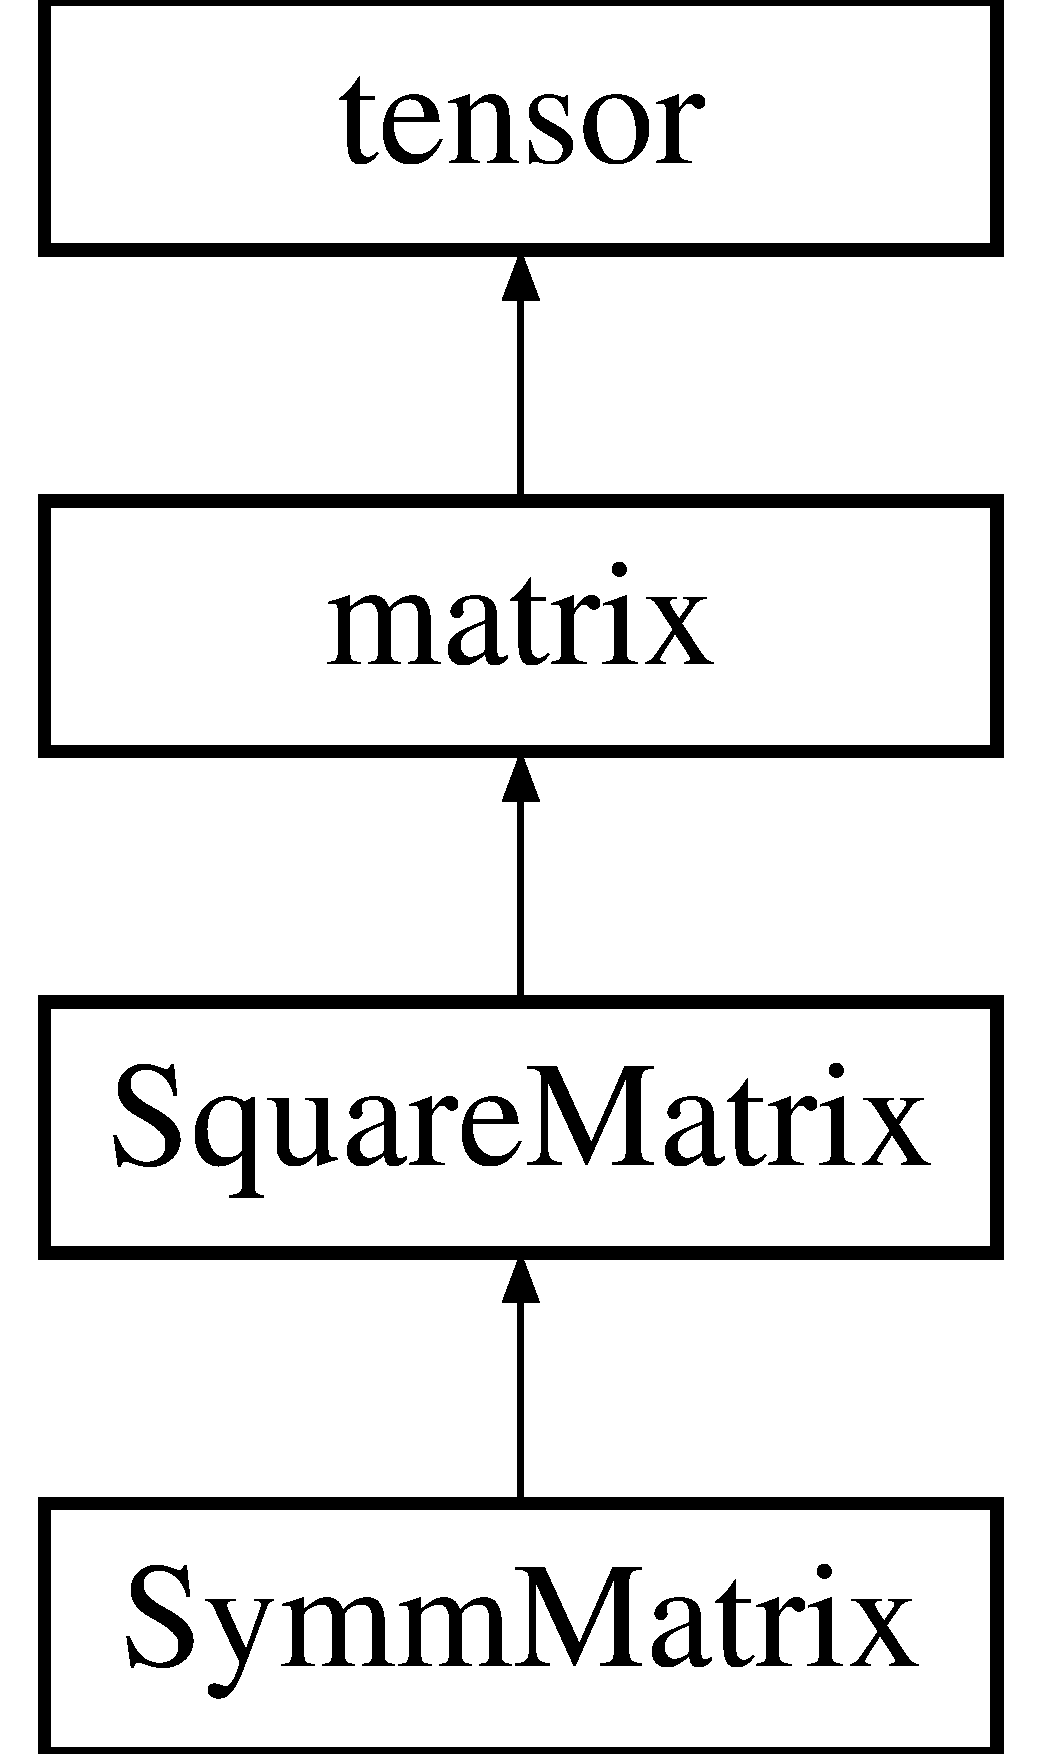
\includegraphics[height=4cm]{classJKBuilder_1_1SymmMatrix}
\end{center}
\end{figure}
\subsection*{Public Member Functions}
\begin{DoxyCompactItemize}
\item 
\hyperlink{classJKBuilder_1_1SymmMatrix_a0232cfa05984c1f35917eff2a56a77dc}{SymmMatrix} (const int n, const bool Init=false)
\begin{DoxyCompactList}\small\item\em Allocates (and sets to 0 if Init==true) an n by n \hyperlink{classJKBuilder_1_1matrix}{matrix}. \item\end{DoxyCompactList}\item 
\hyperlink{classJKBuilder_1_1SymmMatrix_a772cb659e7f24da6add4891fe3a176e2}{SymmMatrix} (const double $\ast$DaMatrix, const int n)
\begin{DoxyCompactList}\small\item\em Makes an n by n \hyperlink{classJKBuilder_1_1matrix}{matrix} by copying DaMatrix. \item\end{DoxyCompactList}\item 
\hyperlink{classJKBuilder_1_1SymmMatrix_a485694eb867a2f935521aa7cc869dd25}{SymmMatrix} (double $\ast$DaMatrix, const int n)
\begin{DoxyCompactList}\small\item\em Sets this \hyperlink{classJKBuilder_1_1matrix}{matrix} equal to the n by n \hyperlink{classJKBuilder_1_1matrix}{matrix} DaMatrix. \item\end{DoxyCompactList}\item 
\hyperlink{classJKBuilder_1_1SymmMatrix_aee15e64745fb95965ac5a526a70a7330}{SymmMatrix} (const \hyperlink{classJKBuilder_1_1SymmMatrix}{SymmMatrix} \&other)
\begin{DoxyCompactList}\small\item\em Makes this \hyperlink{classJKBuilder_1_1matrix}{matrix} a copy of other. \item\end{DoxyCompactList}\item 
\hyperlink{classJKBuilder_1_1SymmMatrix}{SymmMatrix} \& \hyperlink{classJKBuilder_1_1SymmMatrix_aca4a8297278ff39c5422febf1dcbc5ac}{operator=} (const \hyperlink{classJKBuilder_1_1SymmMatrix}{SymmMatrix} \&other)
\begin{DoxyCompactList}\small\item\em Makes this \hyperlink{classJKBuilder_1_1matrix}{matrix} equal to the other one. \item\end{DoxyCompactList}\item 
const double \& \hyperlink{classJKBuilder_1_1SymmMatrix_a9ccbac42f4eefb704f04886001f4fb3e}{operator()} (const int i, const int j) const 
\begin{DoxyCompactList}\small\item\em Returns a non-\/editable element (i,j). \item\end{DoxyCompactList}\item 
double \& \hyperlink{classJKBuilder_1_1SymmMatrix_a3d7fca183ff1c9f4c160218746f2ef31}{operator()} (const int i, const int j)
\begin{DoxyCompactList}\small\item\em Returns an editable element (i,j). \item\end{DoxyCompactList}\item 
void \hyperlink{classJKBuilder_1_1SymmMatrix_ad1dc6c225dae96f6c5f8f91e5462c645}{Symmetrize} ()
\begin{DoxyCompactList}\small\item\em Copies the lower half into the upper half. \item\end{DoxyCompactList}\item 
void \hyperlink{classJKBuilder_1_1matrix_af2563817f6505e9f8a6ee5c5c209a115}{T} ()
\begin{DoxyCompactList}\small\item\em Transposes a \hyperlink{classJKBuilder_1_1matrix}{matrix} by flipping the flag (don't forget to un-\/transpose it). \item\end{DoxyCompactList}\item 
\hyperlink{classJKBuilder_1_1matrix}{matrix} \& \hyperlink{classJKBuilder_1_1matrix_ad4799cbe4a5d07c77f41857a3ce914a2}{operator$\ast$} (const double alpha)
\begin{DoxyCompactList}\small\item\em Scales a \hyperlink{classJKBuilder_1_1matrix}{matrix} by alpha. \item\end{DoxyCompactList}\item 
void \hyperlink{classJKBuilder_1_1tensor_a0ca5cbe96d2a61f06ae4b543ef84f166}{Alloc} ()
\item 
bool \hyperlink{classJKBuilder_1_1tensor_a79c9a36acc5dbeab94033ca97971dc09}{IsSet} () const 
\begin{DoxyCompactList}\small\item\em Returns true if this \hyperlink{classJKBuilder_1_1tensor}{tensor} is allocated and DimsGood==true (roughly the equiv to asking if this is NULL). \item\end{DoxyCompactList}\item 
virtual void \hyperlink{classJKBuilder_1_1tensor_a98b1050f09da390896f964fb7a892391}{Initialize} ()
\begin{DoxyCompactList}\small\item\em Sets all elements to zero in the \hyperlink{classJKBuilder_1_1tensor}{tensor}, which obviously overwrites the contents. \item\end{DoxyCompactList}\item 
virtual void \hyperlink{classJKBuilder_1_1tensor_a10ffea2bf428adfa3e8319646c44a3c6}{Update} (const double $\ast$Tensor)
\begin{DoxyCompactList}\small\item\em Updates DaTensor so that it is the same as Tensor. \item\end{DoxyCompactList}\item 
int \hyperlink{classJKBuilder_1_1tensor_a537b2f14296e2f0e62f00e1703c5fa08}{TotalElements} ()
\item 
int \hyperlink{classJKBuilder_1_1tensor_a6bdcfca6493bc217b607317dbceb28b2}{DimI} (const int i) const 
\begin{DoxyCompactList}\small\item\em Returns dimension i (counting from 0). \item\end{DoxyCompactList}\item 
void \hyperlink{classJKBuilder_1_1tensor_ace6bcf62c74395ab9e37abc4935f66e0}{SetDimensions} (const int $\ast$DesiredDimensions)
\begin{DoxyCompactList}\small\item\em Copies the dimensions you want (DesiredDimensions), into the \hyperlink{classJKBuilder_1_1tensor_a2ce1e6e0782ddee097f2c4aa2663d3e9}{tensor::dimensions}. Overwrites the contents. \item\end{DoxyCompactList}\item 
virtual void \hyperlink{classJKBuilder_1_1tensor_a388f572c62279f839ee138a9afbdeeb5}{print} ()
\begin{DoxyCompactList}\small\item\em Debugging function that prints the \hyperlink{classJKBuilder_1_1tensor}{tensor} (current model not appropriate for a distributed \hyperlink{classJKBuilder_1_1tensor}{tensor}) to the \hyperlink{classJKBuilder_1_1printer}{printer}. \item\end{DoxyCompactList}\item 
virtual void \hyperlink{classJKBuilder_1_1tensor_a74b2fe351a5444c1325870dc6162f451}{print} (\hyperlink{classJKBuilder_1_1IOManager}{IOManager} \&output)
\begin{DoxyCompactList}\small\item\em Allows the user to select the destination of the printed \hyperlink{classJKBuilder_1_1tensor}{tensor}. \item\end{DoxyCompactList}\item 
const double \& \hyperlink{classJKBuilder_1_1tensor_a4f0dc1b84b580cec49500c70f87e084a}{operator\mbox{[}$\,$\mbox{]}} (const int i) const 
\begin{DoxyCompactList}\small\item\em Returns a non-\/modifiable element i of the \hyperlink{classJKBuilder_1_1tensor}{tensor}. \item\end{DoxyCompactList}\item 
double \& \hyperlink{classJKBuilder_1_1tensor_a38c9fed6b117f7cf8b76785648d76b62}{operator\mbox{[}$\,$\mbox{]}} (const int i)
\begin{DoxyCompactList}\small\item\em Returns a modifiable element i of the \hyperlink{classJKBuilder_1_1tensor}{tensor}. \item\end{DoxyCompactList}\item 
bool \hyperlink{classJKBuilder_1_1tensor_a10ae0b61e655854d12c6465d2b9e3506}{operator==} (const \hyperlink{classJKBuilder_1_1tensor}{tensor} \&other)
\begin{DoxyCompactList}\small\item\em Returns true iff this \hyperlink{classJKBuilder_1_1tensor}{tensor} is equal to the other one. \item\end{DoxyCompactList}\item 
bool \hyperlink{classJKBuilder_1_1tensor_a9b42dd835ddf2eb1a26b5d525b59b2b8}{operator!=} (const \hyperlink{classJKBuilder_1_1tensor}{tensor} \&other)
\begin{DoxyCompactList}\small\item\em Returns the opposite of operator==. \item\end{DoxyCompactList}\item 
const double $\ast$ \hyperlink{classJKBuilder_1_1tensor_a6a4e024f566d3bf9ba32a349afc5bbcf}{Address} () const 
\begin{DoxyCompactList}\small\item\em Returns the starting address of the actual data so that pointers can just be passed. \item\end{DoxyCompactList}\item 
double $\ast$ \hyperlink{classJKBuilder_1_1tensor_ac982d9eb84092bfc13694448dd824cbc}{Address} ()
\end{DoxyCompactItemize}
\subsection*{Protected Member Functions}
\begin{DoxyCompactItemize}
\item 
bool \hyperlink{classJKBuilder_1_1tensor_a6e72344440b411f433eb50171648c2d0}{DimsGood} () const 
\begin{DoxyCompactList}\small\item\em Returns true if the dimensions appear set (dimensions!=NULL \&\& dimensions\mbox{[}i\mbox{]}$>$0 for all i). \item\end{DoxyCompactList}\end{DoxyCompactItemize}
\subsection*{Protected Attributes}
\begin{DoxyCompactItemize}
\item 
bool \hyperlink{classJKBuilder_1_1matrix_a77fa48e57c519482de2ec7ec182b16ef}{IsTransposed}
\begin{DoxyCompactList}\small\item\em A flag that tells us if our \hyperlink{classJKBuilder_1_1matrix}{matrix} is transposed. \item\end{DoxyCompactList}\item 
int \hyperlink{classJKBuilder_1_1tensor_a6cfd95afd0afebd625b889fb6e58371c}{rank}
\begin{DoxyCompactList}\small\item\em This is the rank of the \hyperlink{classJKBuilder_1_1tensor}{tensor}. \item\end{DoxyCompactList}\item 
double $\ast$ \hyperlink{classJKBuilder_1_1tensor_a91f7b1e58c0e5d1a49ddb8b80ab7790e}{DaTensor}
\begin{DoxyCompactList}\small\item\em Realistically we are going to want to use this for doubles, so I am not declaring this a template. \item\end{DoxyCompactList}\item 
int \hyperlink{classJKBuilder_1_1tensor_a23ae6a00bed19d2ad34d439636e797da}{nelements}
\begin{DoxyCompactList}\small\item\em This is the total number of elements in the \hyperlink{classJKBuilder_1_1tensor}{tensor}. \item\end{DoxyCompactList}\item 
int $\ast$ \hyperlink{classJKBuilder_1_1tensor_a2ce1e6e0782ddee097f2c4aa2663d3e9}{dimensions}
\begin{DoxyCompactList}\small\item\em This is the array of \hyperlink{classJKBuilder_1_1tensor}{tensor} dimensions (row,column). \item\end{DoxyCompactList}\end{DoxyCompactItemize}
\subsection*{Private Member Functions}
\begin{DoxyCompactItemize}
\item 
void \hyperlink{classJKBuilder_1_1SymmMatrix_aa9f626f684be5ba6ce49b6a335c2e5fe}{Copy} (const double $\ast$DaMatrix)
\item 
void \hyperlink{classJKBuilder_1_1SymmMatrix_a7be0365900350f51e54969bb1961af8f}{Copy} (const \hyperlink{classJKBuilder_1_1SymmMatrix}{SymmMatrix} \&other)
\begin{DoxyCompactList}\small\item\em The function that actually copies the \hyperlink{classJKBuilder_1_1tensor}{tensor}. Do not use if you just want to pass pointers around, cause it copies (duh...). \item\end{DoxyCompactList}\end{DoxyCompactItemize}


\subsection{Detailed Description}
Generalization of a square \hyperlink{classJKBuilder_1_1matrix}{matrix} to a symmetric \hyperlink{classJKBuilder_1_1matrix}{matrix}. My convention is to only use the lower triangular part of a symmetric \hyperlink{classJKBuilder_1_1matrix}{matrix}. 

\subsection{Constructor \& Destructor Documentation}
\hypertarget{classJKBuilder_1_1SymmMatrix_a0232cfa05984c1f35917eff2a56a77dc}{
\index{JKBuilder::SymmMatrix@{JKBuilder::SymmMatrix}!SymmMatrix@{SymmMatrix}}
\index{SymmMatrix@{SymmMatrix}!JKBuilder::SymmMatrix@{JKBuilder::SymmMatrix}}
\subsubsection[{SymmMatrix}]{\setlength{\rightskip}{0pt plus 5cm}{\bf SymmMatrix} (const int {\em n}, \/  const bool {\em Init} = {\ttfamily false})}}
\label{classJKBuilder_1_1SymmMatrix_a0232cfa05984c1f35917eff2a56a77dc}


Allocates (and sets to 0 if Init==true) an n by n \hyperlink{classJKBuilder_1_1matrix}{matrix}. \hypertarget{classJKBuilder_1_1SymmMatrix_a772cb659e7f24da6add4891fe3a176e2}{
\index{JKBuilder::SymmMatrix@{JKBuilder::SymmMatrix}!SymmMatrix@{SymmMatrix}}
\index{SymmMatrix@{SymmMatrix}!JKBuilder::SymmMatrix@{JKBuilder::SymmMatrix}}
\subsubsection[{SymmMatrix}]{\setlength{\rightskip}{0pt plus 5cm}{\bf SymmMatrix} (const double $\ast$ {\em DaMatrix}, \/  const int {\em n})}}
\label{classJKBuilder_1_1SymmMatrix_a772cb659e7f24da6add4891fe3a176e2}


Makes an n by n \hyperlink{classJKBuilder_1_1matrix}{matrix} by copying DaMatrix. \hypertarget{classJKBuilder_1_1SymmMatrix_a485694eb867a2f935521aa7cc869dd25}{
\index{JKBuilder::SymmMatrix@{JKBuilder::SymmMatrix}!SymmMatrix@{SymmMatrix}}
\index{SymmMatrix@{SymmMatrix}!JKBuilder::SymmMatrix@{JKBuilder::SymmMatrix}}
\subsubsection[{SymmMatrix}]{\setlength{\rightskip}{0pt plus 5cm}{\bf SymmMatrix} (double $\ast$ {\em DaMatrix}, \/  const int {\em n})}}
\label{classJKBuilder_1_1SymmMatrix_a485694eb867a2f935521aa7cc869dd25}


Sets this \hyperlink{classJKBuilder_1_1matrix}{matrix} equal to the n by n \hyperlink{classJKBuilder_1_1matrix}{matrix} DaMatrix. \hypertarget{classJKBuilder_1_1SymmMatrix_aee15e64745fb95965ac5a526a70a7330}{
\index{JKBuilder::SymmMatrix@{JKBuilder::SymmMatrix}!SymmMatrix@{SymmMatrix}}
\index{SymmMatrix@{SymmMatrix}!JKBuilder::SymmMatrix@{JKBuilder::SymmMatrix}}
\subsubsection[{SymmMatrix}]{\setlength{\rightskip}{0pt plus 5cm}{\bf SymmMatrix} (const {\bf SymmMatrix} \& {\em other})}}
\label{classJKBuilder_1_1SymmMatrix_aee15e64745fb95965ac5a526a70a7330}


Makes this \hyperlink{classJKBuilder_1_1matrix}{matrix} a copy of other. 

\subsection{Member Function Documentation}
\hypertarget{classJKBuilder_1_1SymmMatrix_aa9f626f684be5ba6ce49b6a335c2e5fe}{
\index{JKBuilder::SymmMatrix@{JKBuilder::SymmMatrix}!Copy@{Copy}}
\index{Copy@{Copy}!JKBuilder::SymmMatrix@{JKBuilder::SymmMatrix}}
\subsubsection[{Copy}]{\setlength{\rightskip}{0pt plus 5cm}void Copy (const double $\ast$ {\em DaMatrix})\hspace{0.3cm}{\ttfamily  \mbox{[}private\mbox{]}}}}
\label{classJKBuilder_1_1SymmMatrix_aa9f626f684be5ba6ce49b6a335c2e5fe}
\hypertarget{classJKBuilder_1_1SymmMatrix_a7be0365900350f51e54969bb1961af8f}{
\index{JKBuilder::SymmMatrix@{JKBuilder::SymmMatrix}!Copy@{Copy}}
\index{Copy@{Copy}!JKBuilder::SymmMatrix@{JKBuilder::SymmMatrix}}
\subsubsection[{Copy}]{\setlength{\rightskip}{0pt plus 5cm}void Copy (const {\bf SymmMatrix} \& {\em other})\hspace{0.3cm}{\ttfamily  \mbox{[}private\mbox{]}}}}
\label{classJKBuilder_1_1SymmMatrix_a7be0365900350f51e54969bb1961af8f}


The function that actually copies the \hyperlink{classJKBuilder_1_1tensor}{tensor}. Do not use if you just want to pass pointers around, cause it copies (duh...). 

Reimplemented from \hyperlink{classJKBuilder_1_1matrix_a75177328107f96ec679d43fce0a9e866}{matrix}.\hypertarget{classJKBuilder_1_1SymmMatrix_aca4a8297278ff39c5422febf1dcbc5ac}{
\index{JKBuilder::SymmMatrix@{JKBuilder::SymmMatrix}!operator=@{operator=}}
\index{operator=@{operator=}!JKBuilder::SymmMatrix@{JKBuilder::SymmMatrix}}
\subsubsection[{operator=}]{\setlength{\rightskip}{0pt plus 5cm}{\bf SymmMatrix} \& operator= (const {\bf SymmMatrix} \& {\em other})}}
\label{classJKBuilder_1_1SymmMatrix_aca4a8297278ff39c5422febf1dcbc5ac}


Makes this \hyperlink{classJKBuilder_1_1matrix}{matrix} equal to the other one. 

Reimplemented from \hyperlink{classJKBuilder_1_1SquareMatrix_ad78e5a12d26f1984d77a57095bc4d181}{SquareMatrix}.\hypertarget{classJKBuilder_1_1SymmMatrix_a9ccbac42f4eefb704f04886001f4fb3e}{
\index{JKBuilder::SymmMatrix@{JKBuilder::SymmMatrix}!operator()@{operator()}}
\index{operator()@{operator()}!JKBuilder::SymmMatrix@{JKBuilder::SymmMatrix}}
\subsubsection[{operator()}]{\setlength{\rightskip}{0pt plus 5cm}const double \& operator() (const int {\em i}, \/  const int {\em j}) const}}
\label{classJKBuilder_1_1SymmMatrix_a9ccbac42f4eefb704f04886001f4fb3e}


Returns a non-\/editable element (i,j). 

Reimplemented from \hyperlink{classJKBuilder_1_1matrix_a9ccbac42f4eefb704f04886001f4fb3e}{matrix}.\hypertarget{classJKBuilder_1_1SymmMatrix_a3d7fca183ff1c9f4c160218746f2ef31}{
\index{JKBuilder::SymmMatrix@{JKBuilder::SymmMatrix}!operator()@{operator()}}
\index{operator()@{operator()}!JKBuilder::SymmMatrix@{JKBuilder::SymmMatrix}}
\subsubsection[{operator()}]{\setlength{\rightskip}{0pt plus 5cm}double \& operator() (const int {\em i}, \/  const int {\em j})}}
\label{classJKBuilder_1_1SymmMatrix_a3d7fca183ff1c9f4c160218746f2ef31}


Returns an editable element (i,j). 

Reimplemented from \hyperlink{classJKBuilder_1_1matrix_a3d7fca183ff1c9f4c160218746f2ef31}{matrix}.\hypertarget{classJKBuilder_1_1SymmMatrix_ad1dc6c225dae96f6c5f8f91e5462c645}{
\index{JKBuilder::SymmMatrix@{JKBuilder::SymmMatrix}!Symmetrize@{Symmetrize}}
\index{Symmetrize@{Symmetrize}!JKBuilder::SymmMatrix@{JKBuilder::SymmMatrix}}
\subsubsection[{Symmetrize}]{\setlength{\rightskip}{0pt plus 5cm}void Symmetrize ()}}
\label{classJKBuilder_1_1SymmMatrix_ad1dc6c225dae96f6c5f8f91e5462c645}


Copies the lower half into the upper half. \hypertarget{classJKBuilder_1_1matrix_af2563817f6505e9f8a6ee5c5c209a115}{
\index{JKBuilder::SymmMatrix@{JKBuilder::SymmMatrix}!T@{T}}
\index{T@{T}!JKBuilder::SymmMatrix@{JKBuilder::SymmMatrix}}
\subsubsection[{T}]{\setlength{\rightskip}{0pt plus 5cm}void T ()\hspace{0.3cm}{\ttfamily  \mbox{[}inherited\mbox{]}}}}
\label{classJKBuilder_1_1matrix_af2563817f6505e9f8a6ee5c5c209a115}


Transposes a \hyperlink{classJKBuilder_1_1matrix}{matrix} by flipping the flag (don't forget to un-\/transpose it). \hypertarget{classJKBuilder_1_1matrix_ad4799cbe4a5d07c77f41857a3ce914a2}{
\index{JKBuilder::SymmMatrix@{JKBuilder::SymmMatrix}!operator$\ast$@{operator$\ast$}}
\index{operator$\ast$@{operator$\ast$}!JKBuilder::SymmMatrix@{JKBuilder::SymmMatrix}}
\subsubsection[{operator$\ast$}]{\setlength{\rightskip}{0pt plus 5cm}{\bf matrix} \& operator$\ast$ (const double {\em alpha})\hspace{0.3cm}{\ttfamily  \mbox{[}inherited\mbox{]}}}}
\label{classJKBuilder_1_1matrix_ad4799cbe4a5d07c77f41857a3ce914a2}


Scales a \hyperlink{classJKBuilder_1_1matrix}{matrix} by alpha. \hypertarget{classJKBuilder_1_1tensor_a6e72344440b411f433eb50171648c2d0}{
\index{JKBuilder::SymmMatrix@{JKBuilder::SymmMatrix}!DimsGood@{DimsGood}}
\index{DimsGood@{DimsGood}!JKBuilder::SymmMatrix@{JKBuilder::SymmMatrix}}
\subsubsection[{DimsGood}]{\setlength{\rightskip}{0pt plus 5cm}bool DimsGood () const\hspace{0.3cm}{\ttfamily  \mbox{[}protected, inherited\mbox{]}}}}
\label{classJKBuilder_1_1tensor_a6e72344440b411f433eb50171648c2d0}


Returns true if the dimensions appear set (dimensions!=NULL \&\& dimensions\mbox{[}i\mbox{]}$>$0 for all i). \hypertarget{classJKBuilder_1_1tensor_a0ca5cbe96d2a61f06ae4b543ef84f166}{
\index{JKBuilder::SymmMatrix@{JKBuilder::SymmMatrix}!Alloc@{Alloc}}
\index{Alloc@{Alloc}!JKBuilder::SymmMatrix@{JKBuilder::SymmMatrix}}
\subsubsection[{Alloc}]{\setlength{\rightskip}{0pt plus 5cm}void Alloc ()\hspace{0.3cm}{\ttfamily  \mbox{[}inherited\mbox{]}}}}
\label{classJKBuilder_1_1tensor_a0ca5cbe96d2a61f06ae4b543ef84f166}
The following function can never be virtual because base operations of the Tensor depend on them The actual memory allocation call, if DaTensor==NULL allocates the memory \hypertarget{classJKBuilder_1_1tensor_a79c9a36acc5dbeab94033ca97971dc09}{
\index{JKBuilder::SymmMatrix@{JKBuilder::SymmMatrix}!IsSet@{IsSet}}
\index{IsSet@{IsSet}!JKBuilder::SymmMatrix@{JKBuilder::SymmMatrix}}
\subsubsection[{IsSet}]{\setlength{\rightskip}{0pt plus 5cm}bool IsSet () const\hspace{0.3cm}{\ttfamily  \mbox{[}inherited\mbox{]}}}}
\label{classJKBuilder_1_1tensor_a79c9a36acc5dbeab94033ca97971dc09}


Returns true if this \hyperlink{classJKBuilder_1_1tensor}{tensor} is allocated and DimsGood==true (roughly the equiv to asking if this is NULL). \hypertarget{classJKBuilder_1_1tensor_a98b1050f09da390896f964fb7a892391}{
\index{JKBuilder::SymmMatrix@{JKBuilder::SymmMatrix}!Initialize@{Initialize}}
\index{Initialize@{Initialize}!JKBuilder::SymmMatrix@{JKBuilder::SymmMatrix}}
\subsubsection[{Initialize}]{\setlength{\rightskip}{0pt plus 5cm}void Initialize ()\hspace{0.3cm}{\ttfamily  \mbox{[}virtual, inherited\mbox{]}}}}
\label{classJKBuilder_1_1tensor_a98b1050f09da390896f964fb7a892391}


Sets all elements to zero in the \hyperlink{classJKBuilder_1_1tensor}{tensor}, which obviously overwrites the contents. 

Reimplemented in \hyperlink{classJKBuilder_1_1DistributedMatrix_a98b1050f09da390896f964fb7a892391}{DistributedMatrix}.\hypertarget{classJKBuilder_1_1tensor_a10ffea2bf428adfa3e8319646c44a3c6}{
\index{JKBuilder::SymmMatrix@{JKBuilder::SymmMatrix}!Update@{Update}}
\index{Update@{Update}!JKBuilder::SymmMatrix@{JKBuilder::SymmMatrix}}
\subsubsection[{Update}]{\setlength{\rightskip}{0pt plus 5cm}void Update (const double $\ast$ {\em Tensor})\hspace{0.3cm}{\ttfamily  \mbox{[}virtual, inherited\mbox{]}}}}
\label{classJKBuilder_1_1tensor_a10ffea2bf428adfa3e8319646c44a3c6}


Updates DaTensor so that it is the same as Tensor. Update always takes the full Tensor, not a block of it. It is child class's jobs to scatter the data if need be. 

Reimplemented in \hyperlink{classJKBuilder_1_1DistributedMatrix_a6a378face23ba83b2431cb08e8519066}{DistributedMatrix}.\hypertarget{classJKBuilder_1_1tensor_a537b2f14296e2f0e62f00e1703c5fa08}{
\index{JKBuilder::SymmMatrix@{JKBuilder::SymmMatrix}!TotalElements@{TotalElements}}
\index{TotalElements@{TotalElements}!JKBuilder::SymmMatrix@{JKBuilder::SymmMatrix}}
\subsubsection[{TotalElements}]{\setlength{\rightskip}{0pt plus 5cm}int TotalElements ()\hspace{0.3cm}{\ttfamily  \mbox{[}inherited\mbox{]}}}}
\label{classJKBuilder_1_1tensor_a537b2f14296e2f0e62f00e1703c5fa08}
\hypertarget{classJKBuilder_1_1tensor_a6bdcfca6493bc217b607317dbceb28b2}{
\index{JKBuilder::SymmMatrix@{JKBuilder::SymmMatrix}!DimI@{DimI}}
\index{DimI@{DimI}!JKBuilder::SymmMatrix@{JKBuilder::SymmMatrix}}
\subsubsection[{DimI}]{\setlength{\rightskip}{0pt plus 5cm}int DimI (const int {\em i}) const\hspace{0.3cm}{\ttfamily  \mbox{[}inherited\mbox{]}}}}
\label{classJKBuilder_1_1tensor_a6bdcfca6493bc217b607317dbceb28b2}


Returns dimension i (counting from 0). \hypertarget{classJKBuilder_1_1tensor_ace6bcf62c74395ab9e37abc4935f66e0}{
\index{JKBuilder::SymmMatrix@{JKBuilder::SymmMatrix}!SetDimensions@{SetDimensions}}
\index{SetDimensions@{SetDimensions}!JKBuilder::SymmMatrix@{JKBuilder::SymmMatrix}}
\subsubsection[{SetDimensions}]{\setlength{\rightskip}{0pt plus 5cm}void SetDimensions (const int $\ast$ {\em DesiredDimensions})\hspace{0.3cm}{\ttfamily  \mbox{[}inherited\mbox{]}}}}
\label{classJKBuilder_1_1tensor_ace6bcf62c74395ab9e37abc4935f66e0}


Copies the dimensions you want (DesiredDimensions), into the \hyperlink{classJKBuilder_1_1tensor_a2ce1e6e0782ddee097f2c4aa2663d3e9}{tensor::dimensions}. Overwrites the contents. \hypertarget{classJKBuilder_1_1tensor_a388f572c62279f839ee138a9afbdeeb5}{
\index{JKBuilder::SymmMatrix@{JKBuilder::SymmMatrix}!print@{print}}
\index{print@{print}!JKBuilder::SymmMatrix@{JKBuilder::SymmMatrix}}
\subsubsection[{print}]{\setlength{\rightskip}{0pt plus 5cm}void print ()\hspace{0.3cm}{\ttfamily  \mbox{[}virtual, inherited\mbox{]}}}}
\label{classJKBuilder_1_1tensor_a388f572c62279f839ee138a9afbdeeb5}


Debugging function that prints the \hyperlink{classJKBuilder_1_1tensor}{tensor} (current model not appropriate for a distributed \hyperlink{classJKBuilder_1_1tensor}{tensor}) to the \hyperlink{classJKBuilder_1_1printer}{printer}. 

Reimplemented in \hyperlink{classJKBuilder_1_1DistributedMatrix_a388f572c62279f839ee138a9afbdeeb5}{DistributedMatrix}.\hypertarget{classJKBuilder_1_1tensor_a74b2fe351a5444c1325870dc6162f451}{
\index{JKBuilder::SymmMatrix@{JKBuilder::SymmMatrix}!print@{print}}
\index{print@{print}!JKBuilder::SymmMatrix@{JKBuilder::SymmMatrix}}
\subsubsection[{print}]{\setlength{\rightskip}{0pt plus 5cm}void print ({\bf IOManager} \& {\em output})\hspace{0.3cm}{\ttfamily  \mbox{[}virtual, inherited\mbox{]}}}}
\label{classJKBuilder_1_1tensor_a74b2fe351a5444c1325870dc6162f451}


Allows the user to select the destination of the printed \hyperlink{classJKBuilder_1_1tensor}{tensor}. 

Reimplemented in \hyperlink{classJKBuilder_1_1DistributedMatrix_a74b2fe351a5444c1325870dc6162f451}{DistributedMatrix}.\hypertarget{classJKBuilder_1_1tensor_a4f0dc1b84b580cec49500c70f87e084a}{
\index{JKBuilder::SymmMatrix@{JKBuilder::SymmMatrix}!operator\mbox{[}\mbox{]}@{operator[]}}
\index{operator\mbox{[}\mbox{]}@{operator[]}!JKBuilder::SymmMatrix@{JKBuilder::SymmMatrix}}
\subsubsection[{operator[]}]{\setlength{\rightskip}{0pt plus 5cm}const double \& operator\mbox{[}$\,$\mbox{]} (const int {\em i}) const\hspace{0.3cm}{\ttfamily  \mbox{[}inherited\mbox{]}}}}
\label{classJKBuilder_1_1tensor_a4f0dc1b84b580cec49500c70f87e084a}


Returns a non-\/modifiable element i of the \hyperlink{classJKBuilder_1_1tensor}{tensor}. \hypertarget{classJKBuilder_1_1tensor_a38c9fed6b117f7cf8b76785648d76b62}{
\index{JKBuilder::SymmMatrix@{JKBuilder::SymmMatrix}!operator\mbox{[}\mbox{]}@{operator[]}}
\index{operator\mbox{[}\mbox{]}@{operator[]}!JKBuilder::SymmMatrix@{JKBuilder::SymmMatrix}}
\subsubsection[{operator[]}]{\setlength{\rightskip}{0pt plus 5cm}double \& operator\mbox{[}$\,$\mbox{]} (const int {\em i})\hspace{0.3cm}{\ttfamily  \mbox{[}inherited\mbox{]}}}}
\label{classJKBuilder_1_1tensor_a38c9fed6b117f7cf8b76785648d76b62}


Returns a modifiable element i of the \hyperlink{classJKBuilder_1_1tensor}{tensor}. \hypertarget{classJKBuilder_1_1tensor_a10ae0b61e655854d12c6465d2b9e3506}{
\index{JKBuilder::SymmMatrix@{JKBuilder::SymmMatrix}!operator==@{operator==}}
\index{operator==@{operator==}!JKBuilder::SymmMatrix@{JKBuilder::SymmMatrix}}
\subsubsection[{operator==}]{\setlength{\rightskip}{0pt plus 5cm}bool operator== (const {\bf tensor} \& {\em other})\hspace{0.3cm}{\ttfamily  \mbox{[}inherited\mbox{]}}}}
\label{classJKBuilder_1_1tensor_a10ae0b61e655854d12c6465d2b9e3506}


Returns true iff this \hyperlink{classJKBuilder_1_1tensor}{tensor} is equal to the other one. \hypertarget{classJKBuilder_1_1tensor_a9b42dd835ddf2eb1a26b5d525b59b2b8}{
\index{JKBuilder::SymmMatrix@{JKBuilder::SymmMatrix}!operator!=@{operator!=}}
\index{operator!=@{operator!=}!JKBuilder::SymmMatrix@{JKBuilder::SymmMatrix}}
\subsubsection[{operator!=}]{\setlength{\rightskip}{0pt plus 5cm}bool operator!= (const {\bf tensor} \& {\em other})\hspace{0.3cm}{\ttfamily  \mbox{[}inherited\mbox{]}}}}
\label{classJKBuilder_1_1tensor_a9b42dd835ddf2eb1a26b5d525b59b2b8}


Returns the opposite of operator==. \hypertarget{classJKBuilder_1_1tensor_a6a4e024f566d3bf9ba32a349afc5bbcf}{
\index{JKBuilder::SymmMatrix@{JKBuilder::SymmMatrix}!Address@{Address}}
\index{Address@{Address}!JKBuilder::SymmMatrix@{JKBuilder::SymmMatrix}}
\subsubsection[{Address}]{\setlength{\rightskip}{0pt plus 5cm}const double $\ast$ Address () const\hspace{0.3cm}{\ttfamily  \mbox{[}inherited\mbox{]}}}}
\label{classJKBuilder_1_1tensor_a6a4e024f566d3bf9ba32a349afc5bbcf}


Returns the starting address of the actual data so that pointers can just be passed. \hypertarget{classJKBuilder_1_1tensor_ac982d9eb84092bfc13694448dd824cbc}{
\index{JKBuilder::SymmMatrix@{JKBuilder::SymmMatrix}!Address@{Address}}
\index{Address@{Address}!JKBuilder::SymmMatrix@{JKBuilder::SymmMatrix}}
\subsubsection[{Address}]{\setlength{\rightskip}{0pt plus 5cm}double $\ast$ Address ()\hspace{0.3cm}{\ttfamily  \mbox{[}inherited\mbox{]}}}}
\label{classJKBuilder_1_1tensor_ac982d9eb84092bfc13694448dd824cbc}


\subsection{Member Data Documentation}
\hypertarget{classJKBuilder_1_1matrix_a77fa48e57c519482de2ec7ec182b16ef}{
\index{JKBuilder::SymmMatrix@{JKBuilder::SymmMatrix}!IsTransposed@{IsTransposed}}
\index{IsTransposed@{IsTransposed}!JKBuilder::SymmMatrix@{JKBuilder::SymmMatrix}}
\subsubsection[{IsTransposed}]{\setlength{\rightskip}{0pt plus 5cm}bool {\bf IsTransposed}\hspace{0.3cm}{\ttfamily  \mbox{[}protected, inherited\mbox{]}}}}
\label{classJKBuilder_1_1matrix_a77fa48e57c519482de2ec7ec182b16ef}


A flag that tells us if our \hyperlink{classJKBuilder_1_1matrix}{matrix} is transposed. \hypertarget{classJKBuilder_1_1tensor_a6cfd95afd0afebd625b889fb6e58371c}{
\index{JKBuilder::SymmMatrix@{JKBuilder::SymmMatrix}!rank@{rank}}
\index{rank@{rank}!JKBuilder::SymmMatrix@{JKBuilder::SymmMatrix}}
\subsubsection[{rank}]{\setlength{\rightskip}{0pt plus 5cm}int {\bf rank}\hspace{0.3cm}{\ttfamily  \mbox{[}protected, inherited\mbox{]}}}}
\label{classJKBuilder_1_1tensor_a6cfd95afd0afebd625b889fb6e58371c}


This is the rank of the \hyperlink{classJKBuilder_1_1tensor}{tensor}. \hypertarget{classJKBuilder_1_1tensor_a91f7b1e58c0e5d1a49ddb8b80ab7790e}{
\index{JKBuilder::SymmMatrix@{JKBuilder::SymmMatrix}!DaTensor@{DaTensor}}
\index{DaTensor@{DaTensor}!JKBuilder::SymmMatrix@{JKBuilder::SymmMatrix}}
\subsubsection[{DaTensor}]{\setlength{\rightskip}{0pt plus 5cm}double$\ast$ {\bf DaTensor}\hspace{0.3cm}{\ttfamily  \mbox{[}protected, inherited\mbox{]}}}}
\label{classJKBuilder_1_1tensor_a91f7b1e58c0e5d1a49ddb8b80ab7790e}


Realistically we are going to want to use this for doubles, so I am not declaring this a template. \hypertarget{classJKBuilder_1_1tensor_a23ae6a00bed19d2ad34d439636e797da}{
\index{JKBuilder::SymmMatrix@{JKBuilder::SymmMatrix}!nelements@{nelements}}
\index{nelements@{nelements}!JKBuilder::SymmMatrix@{JKBuilder::SymmMatrix}}
\subsubsection[{nelements}]{\setlength{\rightskip}{0pt plus 5cm}int {\bf nelements}\hspace{0.3cm}{\ttfamily  \mbox{[}protected, inherited\mbox{]}}}}
\label{classJKBuilder_1_1tensor_a23ae6a00bed19d2ad34d439636e797da}


This is the total number of elements in the \hyperlink{classJKBuilder_1_1tensor}{tensor}. \hypertarget{classJKBuilder_1_1tensor_a2ce1e6e0782ddee097f2c4aa2663d3e9}{
\index{JKBuilder::SymmMatrix@{JKBuilder::SymmMatrix}!dimensions@{dimensions}}
\index{dimensions@{dimensions}!JKBuilder::SymmMatrix@{JKBuilder::SymmMatrix}}
\subsubsection[{dimensions}]{\setlength{\rightskip}{0pt plus 5cm}int$\ast$ {\bf dimensions}\hspace{0.3cm}{\ttfamily  \mbox{[}protected, inherited\mbox{]}}}}
\label{classJKBuilder_1_1tensor_a2ce1e6e0782ddee097f2c4aa2663d3e9}


This is the array of \hyperlink{classJKBuilder_1_1tensor}{tensor} dimensions (row,column). These dimensions are for the whole object, not blocks of it or anything else like that. What this means is that for say a 12 by 12 \hyperlink{classJKBuilder_1_1matrix}{matrix} distributed in 6 by 6 blocks these values are 12, not 6. 

The documentation for this class was generated from the following files:\begin{DoxyCompactItemize}
\item 
src/\hyperlink{SymmMatrix_8h}{SymmMatrix.h}\item 
src/\hyperlink{SymmMatrix_8cpp}{SymmMatrix.cpp}\end{DoxyCompactItemize}

\hypertarget{classJKBuilder_1_1tensor}{
\section{tensor Class Reference}
\label{classJKBuilder_1_1tensor}\index{JKBuilder::tensor@{JKBuilder::tensor}}
}


The \hyperlink{classJKBuilder_1_1tensor}{tensor} class is meant to serve as a base class for matrices, at some point it is intended to be the base class for other ranks than 2.  


{\ttfamily \#include $<$tensor.h$>$}Inheritance diagram for tensor::\begin{figure}[H]
\begin{center}
\leavevmode
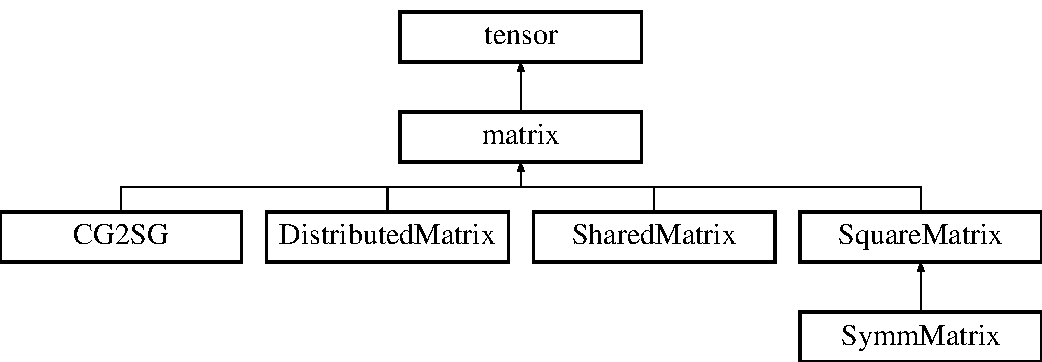
\includegraphics[height=4cm]{classJKBuilder_1_1tensor}
\end{center}
\end{figure}
\subsection*{Public Member Functions}
\begin{DoxyCompactItemize}
\item 
void \hyperlink{classJKBuilder_1_1tensor_a0ca5cbe96d2a61f06ae4b543ef84f166}{Alloc} ()
\item 
bool \hyperlink{classJKBuilder_1_1tensor_a79c9a36acc5dbeab94033ca97971dc09}{IsSet} () const 
\begin{DoxyCompactList}\small\item\em Returns true if this \hyperlink{classJKBuilder_1_1tensor}{tensor} is allocated and DimsGood==true (roughly the equiv to asking if this is NULL). \item\end{DoxyCompactList}\item 
virtual void \hyperlink{classJKBuilder_1_1tensor_a98b1050f09da390896f964fb7a892391}{Initialize} ()
\begin{DoxyCompactList}\small\item\em Sets all elements to zero in the \hyperlink{classJKBuilder_1_1tensor}{tensor}, which obviously overwrites the contents. \item\end{DoxyCompactList}\item 
virtual void \hyperlink{classJKBuilder_1_1tensor_a10ffea2bf428adfa3e8319646c44a3c6}{Update} (const double $\ast$Tensor)
\begin{DoxyCompactList}\small\item\em Updates DaTensor so that it is the same as Tensor. \item\end{DoxyCompactList}\item 
int \hyperlink{classJKBuilder_1_1tensor_a537b2f14296e2f0e62f00e1703c5fa08}{TotalElements} ()
\item 
int \hyperlink{classJKBuilder_1_1tensor_a6bdcfca6493bc217b607317dbceb28b2}{DimI} (const int i) const 
\begin{DoxyCompactList}\small\item\em Returns dimension i (counting from 0). \item\end{DoxyCompactList}\item 
void \hyperlink{classJKBuilder_1_1tensor_ace6bcf62c74395ab9e37abc4935f66e0}{SetDimensions} (const int $\ast$DesiredDimensions)
\begin{DoxyCompactList}\small\item\em Copies the dimensions you want (DesiredDimensions), into the \hyperlink{classJKBuilder_1_1tensor_a2ce1e6e0782ddee097f2c4aa2663d3e9}{tensor::dimensions}. Overwrites the contents. \item\end{DoxyCompactList}\item 
\hyperlink{classJKBuilder_1_1tensor_a35bcdda56953bef8e76bfed569bbf54c}{tensor} (const \hyperlink{classJKBuilder_1_1tensor}{tensor} \&other)
\begin{DoxyCompactList}\small\item\em Copy constructor. \item\end{DoxyCompactList}\item 
\hyperlink{classJKBuilder_1_1tensor_aceb793f098521f84a758cc6f5ff8a997}{tensor} (const int DesiredRank=2)
\begin{DoxyCompactList}\small\item\em Sets the rank to whatever rank you want, which is specified by DesiredRank (defaults to 2). \item\end{DoxyCompactList}\item 
virtual \hyperlink{classJKBuilder_1_1tensor_ac8c25ac32c0d7ab75d3764e014b05997}{$\sim$tensor} ()
\begin{DoxyCompactList}\small\item\em Frees memory associated with \hyperlink{classJKBuilder_1_1tensor_a2ce1e6e0782ddee097f2c4aa2663d3e9}{tensor::dimensions}. \item\end{DoxyCompactList}\item 
virtual void \hyperlink{classJKBuilder_1_1tensor_a388f572c62279f839ee138a9afbdeeb5}{print} ()
\begin{DoxyCompactList}\small\item\em Debugging function that prints the \hyperlink{classJKBuilder_1_1tensor}{tensor} (current model not appropriate for a distributed \hyperlink{classJKBuilder_1_1tensor}{tensor}) to the \hyperlink{classJKBuilder_1_1printer}{printer}. \item\end{DoxyCompactList}\item 
virtual void \hyperlink{classJKBuilder_1_1tensor_a74b2fe351a5444c1325870dc6162f451}{print} (\hyperlink{classJKBuilder_1_1IOManager}{IOManager} \&output)
\begin{DoxyCompactList}\small\item\em Allows the user to select the destination of the printed \hyperlink{classJKBuilder_1_1tensor}{tensor}. \item\end{DoxyCompactList}\item 
const double \& \hyperlink{classJKBuilder_1_1tensor_a4f0dc1b84b580cec49500c70f87e084a}{operator\mbox{[}$\,$\mbox{]}} (const int i) const 
\begin{DoxyCompactList}\small\item\em Returns a non-\/modifiable element i of the \hyperlink{classJKBuilder_1_1tensor}{tensor}. \item\end{DoxyCompactList}\item 
double \& \hyperlink{classJKBuilder_1_1tensor_a38c9fed6b117f7cf8b76785648d76b62}{operator\mbox{[}$\,$\mbox{]}} (const int i)
\begin{DoxyCompactList}\small\item\em Returns a modifiable element i of the \hyperlink{classJKBuilder_1_1tensor}{tensor}. \item\end{DoxyCompactList}\item 
\hyperlink{classJKBuilder_1_1tensor}{tensor} \& \hyperlink{classJKBuilder_1_1tensor_a29113cbfe726b02b94576f631c983386}{operator=} (const \hyperlink{classJKBuilder_1_1tensor}{tensor} \&other)
\begin{DoxyCompactList}\small\item\em Makes this \hyperlink{classJKBuilder_1_1tensor}{tensor} a copy of other. \item\end{DoxyCompactList}\item 
bool \hyperlink{classJKBuilder_1_1tensor_a10ae0b61e655854d12c6465d2b9e3506}{operator==} (const \hyperlink{classJKBuilder_1_1tensor}{tensor} \&other)
\begin{DoxyCompactList}\small\item\em Returns true iff this \hyperlink{classJKBuilder_1_1tensor}{tensor} is equal to the other one. \item\end{DoxyCompactList}\item 
bool \hyperlink{classJKBuilder_1_1tensor_a9b42dd835ddf2eb1a26b5d525b59b2b8}{operator!=} (const \hyperlink{classJKBuilder_1_1tensor}{tensor} \&other)
\begin{DoxyCompactList}\small\item\em Returns the opposite of operator==. \item\end{DoxyCompactList}\item 
const double $\ast$ \hyperlink{classJKBuilder_1_1tensor_a6a4e024f566d3bf9ba32a349afc5bbcf}{Address} () const 
\begin{DoxyCompactList}\small\item\em Returns the starting address of the actual data so that pointers can just be passed. \item\end{DoxyCompactList}\item 
double $\ast$ \hyperlink{classJKBuilder_1_1tensor_ac982d9eb84092bfc13694448dd824cbc}{Address} ()
\end{DoxyCompactItemize}
\subsection*{Protected Member Functions}
\begin{DoxyCompactItemize}
\item 
bool \hyperlink{classJKBuilder_1_1tensor_a6e72344440b411f433eb50171648c2d0}{DimsGood} () const 
\begin{DoxyCompactList}\small\item\em Returns true if the dimensions appear set (dimensions!=NULL \&\& dimensions\mbox{[}i\mbox{]}$>$0 for all i). \item\end{DoxyCompactList}\end{DoxyCompactItemize}
\subsection*{Protected Attributes}
\begin{DoxyCompactItemize}
\item 
int \hyperlink{classJKBuilder_1_1tensor_a6cfd95afd0afebd625b889fb6e58371c}{rank}
\begin{DoxyCompactList}\small\item\em This is the rank of the \hyperlink{classJKBuilder_1_1tensor}{tensor}. \item\end{DoxyCompactList}\item 
double $\ast$ \hyperlink{classJKBuilder_1_1tensor_a91f7b1e58c0e5d1a49ddb8b80ab7790e}{DaTensor}
\begin{DoxyCompactList}\small\item\em Realistically we are going to want to use this for doubles, so I am not declaring this a template. \item\end{DoxyCompactList}\item 
int \hyperlink{classJKBuilder_1_1tensor_a23ae6a00bed19d2ad34d439636e797da}{nelements}
\begin{DoxyCompactList}\small\item\em This is the total number of elements in the \hyperlink{classJKBuilder_1_1tensor}{tensor}. \item\end{DoxyCompactList}\item 
int $\ast$ \hyperlink{classJKBuilder_1_1tensor_a2ce1e6e0782ddee097f2c4aa2663d3e9}{dimensions}
\begin{DoxyCompactList}\small\item\em This is the array of \hyperlink{classJKBuilder_1_1tensor}{tensor} dimensions (row,column). \item\end{DoxyCompactList}\end{DoxyCompactItemize}
\subsection*{Private Member Functions}
\begin{DoxyCompactItemize}
\item 
void \hyperlink{classJKBuilder_1_1tensor_a1b06560e0e01a806b92c2386220d0b57}{SetUp} ()
\begin{DoxyCompactList}\small\item\em This function allocates the memory for the dimensions array and sets nelements to 0. \item\end{DoxyCompactList}\item 
void \hyperlink{classJKBuilder_1_1tensor_a60e1f7417550ba45971b688cc168d34f}{Copy} (const \hyperlink{classJKBuilder_1_1tensor}{tensor} \&other)
\begin{DoxyCompactList}\small\item\em The function that actually copies the \hyperlink{classJKBuilder_1_1tensor}{tensor}. Do not use if you just want to pass pointers around, cause it copies (duh...). \item\end{DoxyCompactList}\end{DoxyCompactItemize}


\subsection{Detailed Description}
The \hyperlink{classJKBuilder_1_1tensor}{tensor} class is meant to serve as a base class for matrices, at some point it is intended to be the base class for other ranks than 2. As of right now I have no need for tensors of rank other than 2 (i.e. matrices) so this best thought of as a base class and not a proper \hyperlink{classJKBuilder_1_1tensor}{tensor}. If and when the need arises, this will be modified to allow for other ranks. 

\subsection{Constructor \& Destructor Documentation}
\hypertarget{classJKBuilder_1_1tensor_a35bcdda56953bef8e76bfed569bbf54c}{
\index{JKBuilder::tensor@{JKBuilder::tensor}!tensor@{tensor}}
\index{tensor@{tensor}!JKBuilder::tensor@{JKBuilder::tensor}}
\subsubsection[{tensor}]{\setlength{\rightskip}{0pt plus 5cm}{\bf tensor} (const {\bf tensor} \& {\em other})}}
\label{classJKBuilder_1_1tensor_a35bcdda56953bef8e76bfed569bbf54c}


Copy constructor. \hypertarget{classJKBuilder_1_1tensor_aceb793f098521f84a758cc6f5ff8a997}{
\index{JKBuilder::tensor@{JKBuilder::tensor}!tensor@{tensor}}
\index{tensor@{tensor}!JKBuilder::tensor@{JKBuilder::tensor}}
\subsubsection[{tensor}]{\setlength{\rightskip}{0pt plus 5cm}{\bf tensor} (const int {\em DesiredRank} = {\ttfamily 2})}}
\label{classJKBuilder_1_1tensor_aceb793f098521f84a758cc6f5ff8a997}


Sets the rank to whatever rank you want, which is specified by DesiredRank (defaults to 2). \hypertarget{classJKBuilder_1_1tensor_ac8c25ac32c0d7ab75d3764e014b05997}{
\index{JKBuilder::tensor@{JKBuilder::tensor}!$\sim$tensor@{$\sim$tensor}}
\index{$\sim$tensor@{$\sim$tensor}!JKBuilder::tensor@{JKBuilder::tensor}}
\subsubsection[{$\sim$tensor}]{\setlength{\rightskip}{0pt plus 5cm}$\sim${\bf tensor} ()\hspace{0.3cm}{\ttfamily  \mbox{[}virtual\mbox{]}}}}
\label{classJKBuilder_1_1tensor_ac8c25ac32c0d7ab75d3764e014b05997}


Frees memory associated with \hyperlink{classJKBuilder_1_1tensor_a2ce1e6e0782ddee097f2c4aa2663d3e9}{tensor::dimensions}. 

\subsection{Member Function Documentation}
\hypertarget{classJKBuilder_1_1tensor_a1b06560e0e01a806b92c2386220d0b57}{
\index{JKBuilder::tensor@{JKBuilder::tensor}!SetUp@{SetUp}}
\index{SetUp@{SetUp}!JKBuilder::tensor@{JKBuilder::tensor}}
\subsubsection[{SetUp}]{\setlength{\rightskip}{0pt plus 5cm}void SetUp ()\hspace{0.3cm}{\ttfamily  \mbox{[}private\mbox{]}}}}
\label{classJKBuilder_1_1tensor_a1b06560e0e01a806b92c2386220d0b57}


This function allocates the memory for the dimensions array and sets nelements to 0. \hypertarget{classJKBuilder_1_1tensor_a60e1f7417550ba45971b688cc168d34f}{
\index{JKBuilder::tensor@{JKBuilder::tensor}!Copy@{Copy}}
\index{Copy@{Copy}!JKBuilder::tensor@{JKBuilder::tensor}}
\subsubsection[{Copy}]{\setlength{\rightskip}{0pt plus 5cm}void Copy (const {\bf tensor} \& {\em other})\hspace{0.3cm}{\ttfamily  \mbox{[}private\mbox{]}}}}
\label{classJKBuilder_1_1tensor_a60e1f7417550ba45971b688cc168d34f}


The function that actually copies the \hyperlink{classJKBuilder_1_1tensor}{tensor}. Do not use if you just want to pass pointers around, cause it copies (duh...). 

Reimplemented in \hyperlink{classJKBuilder_1_1matrix_a75177328107f96ec679d43fce0a9e866}{matrix}, and \hyperlink{classJKBuilder_1_1SymmMatrix_a7be0365900350f51e54969bb1961af8f}{SymmMatrix}.\hypertarget{classJKBuilder_1_1tensor_a6e72344440b411f433eb50171648c2d0}{
\index{JKBuilder::tensor@{JKBuilder::tensor}!DimsGood@{DimsGood}}
\index{DimsGood@{DimsGood}!JKBuilder::tensor@{JKBuilder::tensor}}
\subsubsection[{DimsGood}]{\setlength{\rightskip}{0pt plus 5cm}bool DimsGood () const\hspace{0.3cm}{\ttfamily  \mbox{[}protected\mbox{]}}}}
\label{classJKBuilder_1_1tensor_a6e72344440b411f433eb50171648c2d0}


Returns true if the dimensions appear set (dimensions!=NULL \&\& dimensions\mbox{[}i\mbox{]}$>$0 for all i). \hypertarget{classJKBuilder_1_1tensor_a0ca5cbe96d2a61f06ae4b543ef84f166}{
\index{JKBuilder::tensor@{JKBuilder::tensor}!Alloc@{Alloc}}
\index{Alloc@{Alloc}!JKBuilder::tensor@{JKBuilder::tensor}}
\subsubsection[{Alloc}]{\setlength{\rightskip}{0pt plus 5cm}void Alloc ()}}
\label{classJKBuilder_1_1tensor_a0ca5cbe96d2a61f06ae4b543ef84f166}
The following function can never be virtual because base operations of the Tensor depend on them The actual memory allocation call, if DaTensor==NULL allocates the memory \hypertarget{classJKBuilder_1_1tensor_a79c9a36acc5dbeab94033ca97971dc09}{
\index{JKBuilder::tensor@{JKBuilder::tensor}!IsSet@{IsSet}}
\index{IsSet@{IsSet}!JKBuilder::tensor@{JKBuilder::tensor}}
\subsubsection[{IsSet}]{\setlength{\rightskip}{0pt plus 5cm}bool IsSet () const}}
\label{classJKBuilder_1_1tensor_a79c9a36acc5dbeab94033ca97971dc09}


Returns true if this \hyperlink{classJKBuilder_1_1tensor}{tensor} is allocated and DimsGood==true (roughly the equiv to asking if this is NULL). \hypertarget{classJKBuilder_1_1tensor_a98b1050f09da390896f964fb7a892391}{
\index{JKBuilder::tensor@{JKBuilder::tensor}!Initialize@{Initialize}}
\index{Initialize@{Initialize}!JKBuilder::tensor@{JKBuilder::tensor}}
\subsubsection[{Initialize}]{\setlength{\rightskip}{0pt plus 5cm}void Initialize ()\hspace{0.3cm}{\ttfamily  \mbox{[}virtual\mbox{]}}}}
\label{classJKBuilder_1_1tensor_a98b1050f09da390896f964fb7a892391}


Sets all elements to zero in the \hyperlink{classJKBuilder_1_1tensor}{tensor}, which obviously overwrites the contents. 

Reimplemented in \hyperlink{classJKBuilder_1_1DistributedMatrix_a98b1050f09da390896f964fb7a892391}{DistributedMatrix}.\hypertarget{classJKBuilder_1_1tensor_a10ffea2bf428adfa3e8319646c44a3c6}{
\index{JKBuilder::tensor@{JKBuilder::tensor}!Update@{Update}}
\index{Update@{Update}!JKBuilder::tensor@{JKBuilder::tensor}}
\subsubsection[{Update}]{\setlength{\rightskip}{0pt plus 5cm}void Update (const double $\ast$ {\em Tensor})\hspace{0.3cm}{\ttfamily  \mbox{[}virtual\mbox{]}}}}
\label{classJKBuilder_1_1tensor_a10ffea2bf428adfa3e8319646c44a3c6}


Updates DaTensor so that it is the same as Tensor. Update always takes the full Tensor, not a block of it. It is child class's jobs to scatter the data if need be. 

Reimplemented in \hyperlink{classJKBuilder_1_1DistributedMatrix_a6a378face23ba83b2431cb08e8519066}{DistributedMatrix}.\hypertarget{classJKBuilder_1_1tensor_a537b2f14296e2f0e62f00e1703c5fa08}{
\index{JKBuilder::tensor@{JKBuilder::tensor}!TotalElements@{TotalElements}}
\index{TotalElements@{TotalElements}!JKBuilder::tensor@{JKBuilder::tensor}}
\subsubsection[{TotalElements}]{\setlength{\rightskip}{0pt plus 5cm}int TotalElements ()}}
\label{classJKBuilder_1_1tensor_a537b2f14296e2f0e62f00e1703c5fa08}
\hypertarget{classJKBuilder_1_1tensor_a6bdcfca6493bc217b607317dbceb28b2}{
\index{JKBuilder::tensor@{JKBuilder::tensor}!DimI@{DimI}}
\index{DimI@{DimI}!JKBuilder::tensor@{JKBuilder::tensor}}
\subsubsection[{DimI}]{\setlength{\rightskip}{0pt plus 5cm}int DimI (const int {\em i}) const}}
\label{classJKBuilder_1_1tensor_a6bdcfca6493bc217b607317dbceb28b2}


Returns dimension i (counting from 0). \hypertarget{classJKBuilder_1_1tensor_ace6bcf62c74395ab9e37abc4935f66e0}{
\index{JKBuilder::tensor@{JKBuilder::tensor}!SetDimensions@{SetDimensions}}
\index{SetDimensions@{SetDimensions}!JKBuilder::tensor@{JKBuilder::tensor}}
\subsubsection[{SetDimensions}]{\setlength{\rightskip}{0pt plus 5cm}void SetDimensions (const int $\ast$ {\em DesiredDimensions})}}
\label{classJKBuilder_1_1tensor_ace6bcf62c74395ab9e37abc4935f66e0}


Copies the dimensions you want (DesiredDimensions), into the \hyperlink{classJKBuilder_1_1tensor_a2ce1e6e0782ddee097f2c4aa2663d3e9}{tensor::dimensions}. Overwrites the contents. \hypertarget{classJKBuilder_1_1tensor_a388f572c62279f839ee138a9afbdeeb5}{
\index{JKBuilder::tensor@{JKBuilder::tensor}!print@{print}}
\index{print@{print}!JKBuilder::tensor@{JKBuilder::tensor}}
\subsubsection[{print}]{\setlength{\rightskip}{0pt plus 5cm}void print ()\hspace{0.3cm}{\ttfamily  \mbox{[}virtual\mbox{]}}}}
\label{classJKBuilder_1_1tensor_a388f572c62279f839ee138a9afbdeeb5}


Debugging function that prints the \hyperlink{classJKBuilder_1_1tensor}{tensor} (current model not appropriate for a distributed \hyperlink{classJKBuilder_1_1tensor}{tensor}) to the \hyperlink{classJKBuilder_1_1printer}{printer}. 

Reimplemented in \hyperlink{classJKBuilder_1_1DistributedMatrix_a388f572c62279f839ee138a9afbdeeb5}{DistributedMatrix}.\hypertarget{classJKBuilder_1_1tensor_a74b2fe351a5444c1325870dc6162f451}{
\index{JKBuilder::tensor@{JKBuilder::tensor}!print@{print}}
\index{print@{print}!JKBuilder::tensor@{JKBuilder::tensor}}
\subsubsection[{print}]{\setlength{\rightskip}{0pt plus 5cm}void print ({\bf IOManager} \& {\em output})\hspace{0.3cm}{\ttfamily  \mbox{[}virtual\mbox{]}}}}
\label{classJKBuilder_1_1tensor_a74b2fe351a5444c1325870dc6162f451}


Allows the user to select the destination of the printed \hyperlink{classJKBuilder_1_1tensor}{tensor}. 

Reimplemented in \hyperlink{classJKBuilder_1_1DistributedMatrix_a74b2fe351a5444c1325870dc6162f451}{DistributedMatrix}.\hypertarget{classJKBuilder_1_1tensor_a4f0dc1b84b580cec49500c70f87e084a}{
\index{JKBuilder::tensor@{JKBuilder::tensor}!operator\mbox{[}\mbox{]}@{operator[]}}
\index{operator\mbox{[}\mbox{]}@{operator[]}!JKBuilder::tensor@{JKBuilder::tensor}}
\subsubsection[{operator[]}]{\setlength{\rightskip}{0pt plus 5cm}const double \& operator\mbox{[}$\,$\mbox{]} (const int {\em i}) const}}
\label{classJKBuilder_1_1tensor_a4f0dc1b84b580cec49500c70f87e084a}


Returns a non-\/modifiable element i of the \hyperlink{classJKBuilder_1_1tensor}{tensor}. \hypertarget{classJKBuilder_1_1tensor_a38c9fed6b117f7cf8b76785648d76b62}{
\index{JKBuilder::tensor@{JKBuilder::tensor}!operator\mbox{[}\mbox{]}@{operator[]}}
\index{operator\mbox{[}\mbox{]}@{operator[]}!JKBuilder::tensor@{JKBuilder::tensor}}
\subsubsection[{operator[]}]{\setlength{\rightskip}{0pt plus 5cm}double \& operator\mbox{[}$\,$\mbox{]} (const int {\em i})}}
\label{classJKBuilder_1_1tensor_a38c9fed6b117f7cf8b76785648d76b62}


Returns a modifiable element i of the \hyperlink{classJKBuilder_1_1tensor}{tensor}. \hypertarget{classJKBuilder_1_1tensor_a29113cbfe726b02b94576f631c983386}{
\index{JKBuilder::tensor@{JKBuilder::tensor}!operator=@{operator=}}
\index{operator=@{operator=}!JKBuilder::tensor@{JKBuilder::tensor}}
\subsubsection[{operator=}]{\setlength{\rightskip}{0pt plus 5cm}{\bf tensor} \& operator= (const {\bf tensor} \& {\em other})}}
\label{classJKBuilder_1_1tensor_a29113cbfe726b02b94576f631c983386}


Makes this \hyperlink{classJKBuilder_1_1tensor}{tensor} a copy of other. 

Reimplemented in \hyperlink{classJKBuilder_1_1matrix_a11df53cc3fc568369a9f612cfb556680}{matrix}, \hyperlink{classJKBuilder_1_1SquareMatrix_ad78e5a12d26f1984d77a57095bc4d181}{SquareMatrix}, and \hyperlink{classJKBuilder_1_1SymmMatrix_aca4a8297278ff39c5422febf1dcbc5ac}{SymmMatrix}.\hypertarget{classJKBuilder_1_1tensor_a10ae0b61e655854d12c6465d2b9e3506}{
\index{JKBuilder::tensor@{JKBuilder::tensor}!operator==@{operator==}}
\index{operator==@{operator==}!JKBuilder::tensor@{JKBuilder::tensor}}
\subsubsection[{operator==}]{\setlength{\rightskip}{0pt plus 5cm}bool operator== (const {\bf tensor} \& {\em other})}}
\label{classJKBuilder_1_1tensor_a10ae0b61e655854d12c6465d2b9e3506}


Returns true iff this \hyperlink{classJKBuilder_1_1tensor}{tensor} is equal to the other one. \hypertarget{classJKBuilder_1_1tensor_a9b42dd835ddf2eb1a26b5d525b59b2b8}{
\index{JKBuilder::tensor@{JKBuilder::tensor}!operator!=@{operator!=}}
\index{operator!=@{operator!=}!JKBuilder::tensor@{JKBuilder::tensor}}
\subsubsection[{operator!=}]{\setlength{\rightskip}{0pt plus 5cm}bool operator!= (const {\bf tensor} \& {\em other})}}
\label{classJKBuilder_1_1tensor_a9b42dd835ddf2eb1a26b5d525b59b2b8}


Returns the opposite of operator==. \hypertarget{classJKBuilder_1_1tensor_a6a4e024f566d3bf9ba32a349afc5bbcf}{
\index{JKBuilder::tensor@{JKBuilder::tensor}!Address@{Address}}
\index{Address@{Address}!JKBuilder::tensor@{JKBuilder::tensor}}
\subsubsection[{Address}]{\setlength{\rightskip}{0pt plus 5cm}const double $\ast$ Address () const}}
\label{classJKBuilder_1_1tensor_a6a4e024f566d3bf9ba32a349afc5bbcf}


Returns the starting address of the actual data so that pointers can just be passed. \hypertarget{classJKBuilder_1_1tensor_ac982d9eb84092bfc13694448dd824cbc}{
\index{JKBuilder::tensor@{JKBuilder::tensor}!Address@{Address}}
\index{Address@{Address}!JKBuilder::tensor@{JKBuilder::tensor}}
\subsubsection[{Address}]{\setlength{\rightskip}{0pt plus 5cm}double $\ast$ Address ()}}
\label{classJKBuilder_1_1tensor_ac982d9eb84092bfc13694448dd824cbc}


\subsection{Member Data Documentation}
\hypertarget{classJKBuilder_1_1tensor_a6cfd95afd0afebd625b889fb6e58371c}{
\index{JKBuilder::tensor@{JKBuilder::tensor}!rank@{rank}}
\index{rank@{rank}!JKBuilder::tensor@{JKBuilder::tensor}}
\subsubsection[{rank}]{\setlength{\rightskip}{0pt plus 5cm}int {\bf rank}\hspace{0.3cm}{\ttfamily  \mbox{[}protected\mbox{]}}}}
\label{classJKBuilder_1_1tensor_a6cfd95afd0afebd625b889fb6e58371c}


This is the rank of the \hyperlink{classJKBuilder_1_1tensor}{tensor}. \hypertarget{classJKBuilder_1_1tensor_a91f7b1e58c0e5d1a49ddb8b80ab7790e}{
\index{JKBuilder::tensor@{JKBuilder::tensor}!DaTensor@{DaTensor}}
\index{DaTensor@{DaTensor}!JKBuilder::tensor@{JKBuilder::tensor}}
\subsubsection[{DaTensor}]{\setlength{\rightskip}{0pt plus 5cm}double$\ast$ {\bf DaTensor}\hspace{0.3cm}{\ttfamily  \mbox{[}protected\mbox{]}}}}
\label{classJKBuilder_1_1tensor_a91f7b1e58c0e5d1a49ddb8b80ab7790e}


Realistically we are going to want to use this for doubles, so I am not declaring this a template. \hypertarget{classJKBuilder_1_1tensor_a23ae6a00bed19d2ad34d439636e797da}{
\index{JKBuilder::tensor@{JKBuilder::tensor}!nelements@{nelements}}
\index{nelements@{nelements}!JKBuilder::tensor@{JKBuilder::tensor}}
\subsubsection[{nelements}]{\setlength{\rightskip}{0pt plus 5cm}int {\bf nelements}\hspace{0.3cm}{\ttfamily  \mbox{[}protected\mbox{]}}}}
\label{classJKBuilder_1_1tensor_a23ae6a00bed19d2ad34d439636e797da}


This is the total number of elements in the \hyperlink{classJKBuilder_1_1tensor}{tensor}. \hypertarget{classJKBuilder_1_1tensor_a2ce1e6e0782ddee097f2c4aa2663d3e9}{
\index{JKBuilder::tensor@{JKBuilder::tensor}!dimensions@{dimensions}}
\index{dimensions@{dimensions}!JKBuilder::tensor@{JKBuilder::tensor}}
\subsubsection[{dimensions}]{\setlength{\rightskip}{0pt plus 5cm}int$\ast$ {\bf dimensions}\hspace{0.3cm}{\ttfamily  \mbox{[}protected\mbox{]}}}}
\label{classJKBuilder_1_1tensor_a2ce1e6e0782ddee097f2c4aa2663d3e9}


This is the array of \hyperlink{classJKBuilder_1_1tensor}{tensor} dimensions (row,column). These dimensions are for the whole object, not blocks of it or anything else like that. What this means is that for say a 12 by 12 \hyperlink{classJKBuilder_1_1matrix}{matrix} distributed in 6 by 6 blocks these values are 12, not 6. 

The documentation for this class was generated from the following files:\begin{DoxyCompactItemize}
\item 
src/\hyperlink{tensor_8h}{tensor.h}\item 
src/\hyperlink{tensor_8cpp}{tensor.cpp}\end{DoxyCompactItemize}

\chapter{File Documentation}
\hypertarget{README_8dox}{
\section{README.dox File Reference}
\label{README_8dox}\index{README.dox@{README.dox}}
}

\hypertarget{BasisSet_8cpp}{
\section{src/BasisSet.cpp File Reference}
\label{BasisSet_8cpp}\index{src/BasisSet.cpp@{src/BasisSet.cpp}}
}
{\ttfamily \#include \char`\"{}molecule.h\char`\"{}}\par
{\ttfamily \#include \char`\"{}BasisSet.h\char`\"{}}\par
{\ttfamily \#include \char`\"{}JKBuilder.h\char`\"{}}\par
\subsection*{Namespaces}
\begin{DoxyCompactItemize}
\item 
namespace \hyperlink{namespaceJKBuilder}{JKBuilder}
\end{DoxyCompactItemize}

\hypertarget{BasisSet_8h}{
\section{src/BasisSet.h File Reference}
\label{BasisSet_8h}\index{src/BasisSet.h@{src/BasisSet.h}}
}
{\ttfamily \#include $<$vector$>$}\par
\subsection*{Classes}
\begin{DoxyCompactItemize}
\item 
class \hyperlink{classJKBuilder_1_1Primitive}{Primitive}
\begin{DoxyCompactList}\small\item\em A Gaussian primitive. \item\end{DoxyCompactList}\item 
class \hyperlink{classJKBuilder_1_1Shell}{Shell}
\begin{DoxyCompactList}\small\item\em A shell of Gaussian primitives. \item\end{DoxyCompactList}\item 
class \hyperlink{classJKBuilder_1_1CartShell}{CartShell}
\begin{DoxyCompactList}\small\item\em Specialization of \hyperlink{classJKBuilder_1_1Shell}{Shell} to Cartesian Gaussians. \item\end{DoxyCompactList}\item 
class \hyperlink{classJKBuilder_1_1SphereShell}{SphereShell}
\begin{DoxyCompactList}\small\item\em Specialization of \hyperlink{classJKBuilder_1_1Shell}{Shell} to Spherical Gaussians. \item\end{DoxyCompactList}\item 
class \hyperlink{classJKBuilder_1_1BasisSet}{BasisSet}
\begin{DoxyCompactList}\small\item\em An abstract base class for Gaussian basis sets. \item\end{DoxyCompactList}\item 
class \hyperlink{classJKBuilder_1_1AtomicBasisSet}{AtomicBasisSet}
\item 
class \hyperlink{classJKBuilder_1_1AOBasisSet}{AOBasisSet}
\begin{DoxyCompactList}\small\item\em The top-\/level basis set object for the \hyperlink{namespaceJKBuilder}{JKBuilder} library. \item\end{DoxyCompactList}\end{DoxyCompactItemize}
\subsection*{Namespaces}
\begin{DoxyCompactItemize}
\item 
namespace \hyperlink{namespaceJKBuilder}{JKBuilder}
\end{DoxyCompactItemize}

\hypertarget{CG2SG_8cpp}{
\section{src/CG2SG.cpp File Reference}
\label{CG2SG_8cpp}\index{src/CG2SG.cpp@{src/CG2SG.cpp}}
}
{\ttfamily \#include \char`\"{}CG2SG.h\char`\"{}}\par
{\ttfamily \#include \char`\"{}BasisSet.h\char`\"{}}\par
{\ttfamily \#include $<$cmath$>$}\par
\subsection*{Namespaces}
\begin{DoxyCompactItemize}
\item 
namespace \hyperlink{namespaceJKBuilder}{JKBuilder}
\end{DoxyCompactItemize}
\subsection*{Typedefs}
\begin{DoxyCompactItemize}
\item 
typedef unsigned long \hyperlink{namespaceJKBuilder_af632da489ebc3708ec3ab6791ee53fa4}{ULONG}
\end{DoxyCompactItemize}
\subsection*{Functions}
\begin{DoxyCompactItemize}
\item 
ULONG \hyperlink{namespaceJKBuilder_aa1788c8c311e8c98d9db3c6b8094570c}{binomial} (ULONG n, ULONG k)
\item 
ULONG \hyperlink{namespaceJKBuilder_a0abd753c6677358f15ae5ef2bc41dd4f}{factorial} (ULONG m)
\end{DoxyCompactItemize}

\hypertarget{CG2SG_8h}{
\section{src/CG2SG.h File Reference}
\label{CG2SG_8h}\index{src/CG2SG.h@{src/CG2SG.h}}
}
{\ttfamily \#include \char`\"{}matrix.h\char`\"{}}\par
\subsection*{Classes}
\begin{DoxyCompactItemize}
\item 
class \hyperlink{classJKBuilder_1_1CG2SG}{CG2SG}
\begin{DoxyCompactList}\small\item\em This class handles the transformation from Cartesian Gaussians to Spherical Gaussians. \item\end{DoxyCompactList}\end{DoxyCompactItemize}
\subsection*{Namespaces}
\begin{DoxyCompactItemize}
\item 
namespace \hyperlink{namespaceJKBuilder}{JKBuilder}
\end{DoxyCompactItemize}

\hypertarget{DistGTFock_8cpp}{
\section{src/DistGTFock.cpp File Reference}
\label{DistGTFock_8cpp}\index{src/DistGTFock.cpp@{src/DistGTFock.cpp}}
}
{\ttfamily \#include \char`\"{}DistGTFock.h\char`\"{}}\par
{\ttfamily \#include \char`\"{}molecule.h\char`\"{}}\par
{\ttfamily \#include \char`\"{}MPIManager.h\char`\"{}}\par
{\ttfamily \#include \char`\"{}JKBuilder.h\char`\"{}}\par
{\ttfamily \#include $<$cmath$>$}\par
{\ttfamily \#include $<$cstdlib$>$}\par
{\ttfamily \#include \char`\"{}include/CInt.h\char`\"{}}\par
{\ttfamily \#include \char`\"{}libcint/cint\_\-type.h\char`\"{}}\par
{\ttfamily \#include \char`\"{}include/PFock.h\char`\"{}}\par
{\ttfamily \#include \char`\"{}libpfock/pfock\_\-type.h\char`\"{}}\par
{\ttfamily \#include \char`\"{}DistributedMatrix.h\char`\"{}}\par
{\ttfamily \#include \char`\"{}FileManager.h\char`\"{}}\par
{\ttfamily \#include \char`\"{}BasisSet.h\char`\"{}}\par
{\ttfamily \#include \char`\"{}SymmMatrix.h\char`\"{}}\par
\subsection*{Namespaces}
\begin{DoxyCompactItemize}
\item 
namespace \hyperlink{namespaceGTFock}{GTFock}


\begin{DoxyCompactList}\small\item\em The class that implements distributed arrays with the \hyperlink{namespaceGTFock}{GTFock} library. \item\end{DoxyCompactList}\end{DoxyCompactItemize}
\subsection*{Functions}
\begin{DoxyCompactItemize}
\item 
void \hyperlink{namespaceGTFock_a9e4cb27d603e3109b98e47f38bc7e3a2}{DebugBasis} (BasisSet $\ast$GTbasis)
\end{DoxyCompactItemize}

\hypertarget{DistGTFock_8h}{
\section{src/DistGTFock.h File Reference}
\label{DistGTFock_8h}\index{src/DistGTFock.h@{src/DistGTFock.h}}
}
{\ttfamily \#include \char`\"{}DistributionCenter.h\char`\"{}}\par
{\ttfamily \#include \char`\"{}JKBuilder.h\char`\"{}}\par
\subsection*{Classes}
\begin{DoxyCompactItemize}
\item 
class \hyperlink{classGTFock_1_1DistGTFock}{DistGTFock}
\end{DoxyCompactItemize}
\subsection*{Namespaces}
\begin{DoxyCompactItemize}
\item 
namespace \hyperlink{namespaceJKBuilder}{JKBuilder}
\item 
namespace \hyperlink{namespaceGTFock}{GTFock}


\begin{DoxyCompactList}\small\item\em The class that implements distributed arrays with the \hyperlink{namespaceGTFock}{GTFock} library. \item\end{DoxyCompactList}\end{DoxyCompactItemize}

\hypertarget{DistributedMatrix_8cpp}{
\section{src/DistributedMatrix.cpp File Reference}
\label{DistributedMatrix_8cpp}\index{src/DistributedMatrix.cpp@{src/DistributedMatrix.cpp}}
}
{\ttfamily \#include \char`\"{}DistributedMatrix.h\char`\"{}}\par
{\ttfamily \#include \char`\"{}MPIManager.h\char`\"{}}\par
{\ttfamily \#include $<$cmath$>$}\par
{\ttfamily \#include $<$stdlib.h$>$}\par
\subsection*{Namespaces}
\begin{DoxyCompactItemize}
\item 
namespace \hyperlink{namespaceJKBuilder}{JKBuilder}
\end{DoxyCompactItemize}
\subsection*{Functions}
\begin{DoxyCompactItemize}
\item 
int \hyperlink{DistributedMatrix_8cpp_aaec66aa7f20c58cce510893341864fa5}{numroc\_\-} (int $\ast$, int $\ast$, int $\ast$, int $\ast$, int $\ast$)
\item 
void \hyperlink{namespaceJKBuilder_aafc94332505e33cee00dd5ace182d2ee}{PrintBlock} (double $\ast$block, int host, int startrow, int startcol, int endrow, int endcol)
\end{DoxyCompactItemize}


\subsection{Function Documentation}
\hypertarget{DistributedMatrix_8cpp_aaec66aa7f20c58cce510893341864fa5}{
\index{DistributedMatrix.cpp@{DistributedMatrix.cpp}!numroc\_\-@{numroc\_\-}}
\index{numroc\_\-@{numroc\_\-}!DistributedMatrix.cpp@{DistributedMatrix.cpp}}
\subsubsection[{numroc\_\-}]{\setlength{\rightskip}{0pt plus 5cm}int numroc\_\- (int $\ast$, \/  int $\ast$, \/  int $\ast$, \/  int $\ast$, \/  int $\ast$)}}
\label{DistributedMatrix_8cpp_aaec66aa7f20c58cce510893341864fa5}

\hypertarget{DistributedMatrix_8h}{
\section{src/DistributedMatrix.h File Reference}
\label{DistributedMatrix_8h}\index{src/DistributedMatrix.h@{src/DistributedMatrix.h}}
}
{\ttfamily \#include \char`\"{}matrix.h\char`\"{}}\par
{\ttfamily \#include $<$boost/smart\_\-ptr/shared\_\-ptr.hpp$>$}\par
\subsection*{Classes}
\begin{DoxyCompactItemize}
\item 
class \hyperlink{classJKBuilder_1_1DistributedMatrix}{DistributedMatrix}
\end{DoxyCompactItemize}
\subsection*{Namespaces}
\begin{DoxyCompactItemize}
\item 
namespace \hyperlink{namespaceJKBuilder}{JKBuilder}
\end{DoxyCompactItemize}
\subsection*{Typedefs}
\begin{DoxyCompactItemize}
\item 
typedef boost::shared\_\-ptr$<$ DistributedMatrix $>$ \hyperlink{namespaceJKBuilder_a3b337e72f5cb0686ec93e063dda09c70}{SharedDistMatrix}
\end{DoxyCompactItemize}

\hypertarget{DistributionCenter_8cpp}{
\section{src/DistributionCenter.cpp File Reference}
\label{DistributionCenter_8cpp}\index{src/DistributionCenter.cpp@{src/DistributionCenter.cpp}}
}
{\ttfamily \#include \char`\"{}DistributionCenter.h\char`\"{}}\par
{\ttfamily \#include \char`\"{}MPIManager.h\char`\"{}}\par
{\ttfamily \#include \char`\"{}BasisSet.h\char`\"{}}\par
{\ttfamily \#include \char`\"{}DistributedMatrix.h\char`\"{}}\par
\subsection*{Namespaces}
\begin{DoxyCompactItemize}
\item 
namespace \hyperlink{namespaceJKBuilder}{JKBuilder}
\end{DoxyCompactItemize}

\hypertarget{DistributionCenter_8h}{
\section{src/DistributionCenter.h File Reference}
\label{DistributionCenter_8h}\index{src/DistributionCenter.h@{src/DistributionCenter.h}}
}
{\ttfamily \#include \char`\"{}JKFactory.h\char`\"{}}\par
{\ttfamily \#include $<$vector$>$}\par
\subsection*{Classes}
\begin{DoxyCompactItemize}
\item 
class \hyperlink{classJKBuilder_1_1DistributionCenter}{DistributionCenter}
\begin{DoxyCompactList}\small\item\em A distribution center is a \hyperlink{classJKBuilder_1_1JKFactory}{JKFactory} that makes distributed objects. \item\end{DoxyCompactList}\end{DoxyCompactItemize}
\subsection*{Namespaces}
\begin{DoxyCompactItemize}
\item 
namespace \hyperlink{namespaceJKBuilder}{JKBuilder}
\end{DoxyCompactItemize}

\hypertarget{EigenMatrixAPI_8h}{
\section{src/EigenMatrixAPI.h File Reference}
\label{EigenMatrixAPI_8h}\index{src/EigenMatrixAPI.h@{src/EigenMatrixAPI.h}}
}
{\ttfamily \#include $<$Eigen/Dense$>$}\par
\subsection*{Namespaces}
\begin{DoxyCompactItemize}
\item 
namespace \hyperlink{namespaceJKBuilder}{JKBuilder}
\end{DoxyCompactItemize}
\subsection*{Defines}
\begin{DoxyCompactItemize}
\item 
\#define \hyperlink{EigenMatrixAPI_8h_a5bd13fea2d52009d82048504cb75e7c1}{EIGEN\_\-USE\_\-MKL\_\-ALL}
\end{DoxyCompactItemize}
\subsection*{Typedefs}
\begin{DoxyCompactItemize}
\item 
typedef Eigen::MatrixXd \hyperlink{namespaceJKBuilder_adfecb398197e2c871cba88a5f9f3c5fe}{Matrix}
\item 
typedef Eigen::Map$<$ Matrix, Eigen::Unaligned, Eigen::RowMajor $>$ \hyperlink{namespaceJKBuilder_a3f2825245708c24ccca9ddcadca9754d}{MatrixWrapper}
\item 
typedef boost::shared\_\-ptr$<$ Matrix $>$ \hyperlink{namespaceJKBuilder_a36fdf7f9a8c81e7ddac62fddb1996ab3}{SharedEigenMatrix}
\item 
typedef boost::shared\_\-ptr$<$ MatrixWrapper $>$ \hyperlink{namespaceJKBuilder_ad018675eed9ebe499b95822286a7e912}{SharedEigenWrapper}
\end{DoxyCompactItemize}


\subsection{Define Documentation}
\hypertarget{EigenMatrixAPI_8h_a5bd13fea2d52009d82048504cb75e7c1}{
\index{EigenMatrixAPI.h@{EigenMatrixAPI.h}!EIGEN\_\-USE\_\-MKL\_\-ALL@{EIGEN\_\-USE\_\-MKL\_\-ALL}}
\index{EIGEN\_\-USE\_\-MKL\_\-ALL@{EIGEN\_\-USE\_\-MKL\_\-ALL}!EigenMatrixAPI.h@{EigenMatrixAPI.h}}
\subsubsection[{EIGEN\_\-USE\_\-MKL\_\-ALL}]{\setlength{\rightskip}{0pt plus 5cm}\#define EIGEN\_\-USE\_\-MKL\_\-ALL}}
\label{EigenMatrixAPI_8h_a5bd13fea2d52009d82048504cb75e7c1}

\hypertarget{FileManager_8cpp}{
\section{src/FileManager.cpp File Reference}
\label{FileManager_8cpp}\index{src/FileManager.cpp@{src/FileManager.cpp}}
}
{\ttfamily \#include \char`\"{}FileManager.h\char`\"{}}\par
{\ttfamily \#include \char`\"{}JKBuilder.h\char`\"{}}\par
{\ttfamily \#include $<$fstream$>$}\par
{\ttfamily \#include $<$boost/filesystem/operations.hpp$>$}\par
\subsection*{Namespaces}
\begin{DoxyCompactItemize}
\item 
namespace \hyperlink{namespaceJKBuilder}{JKBuilder}
\end{DoxyCompactItemize}

\hypertarget{FileManager_8h}{
\section{src/FileManager.h File Reference}
\label{FileManager_8h}\index{src/FileManager.h@{src/FileManager.h}}
}
{\ttfamily \#include \char`\"{}IOManager.h\char`\"{}}\par
{\ttfamily \#include $<$boost/filesystem.hpp$>$}\par
\subsection*{Classes}
\begin{DoxyCompactItemize}
\item 
class \hyperlink{classJKBuilder_1_1FileManager}{FileManager}
\end{DoxyCompactItemize}
\subsection*{Namespaces}
\begin{DoxyCompactItemize}
\item 
namespace \hyperlink{namespaceJKBuilder}{JKBuilder}
\end{DoxyCompactItemize}

\hypertarget{Integrals_8cpp}{
\section{src/Integrals.cpp File Reference}
\label{Integrals_8cpp}\index{src/Integrals.cpp@{src/Integrals.cpp}}
}
{\ttfamily \#include \char`\"{}Integrals.h\char`\"{}}\par
\subsection*{Namespaces}
\begin{DoxyCompactItemize}
\item 
namespace \hyperlink{namespaceJKBuilder}{JKBuilder}
\end{DoxyCompactItemize}

\hypertarget{Integrals_8h}{
\section{src/Integrals.h File Reference}
\label{Integrals_8h}\index{src/Integrals.h@{src/Integrals.h}}
}
{\ttfamily \#include \char`\"{}boost/function.hpp\char`\"{}}\par
{\ttfamily \#include $<$vector$>$}\par
\subsection*{Classes}
\begin{DoxyCompactItemize}
\item 
class \hyperlink{classJKBuilder_1_1Integrals}{Integrals}
\begin{DoxyCompactList}\small\item\em The \hyperlink{classJKBuilder_1_1Integrals}{Integrals} class is an API to the various integral packages that may be used. \item\end{DoxyCompactList}\end{DoxyCompactItemize}
\subsection*{Namespaces}
\begin{DoxyCompactItemize}
\item 
namespace \hyperlink{namespaceJKBuilder}{JKBuilder}
\end{DoxyCompactItemize}
\subsection*{Typedefs}
\begin{DoxyCompactItemize}
\item 
typedef boost::function$<$ int(int P, int Q, int R, int S)$>$ \hyperlink{Integrals_8h_ac8a8046e90f302a56e8d49058926be33}{ComputeFxn}
\item 
typedef boost::function$<$ const double $\ast$()$>$ \hyperlink{Integrals_8h_ab945cefec686042cf6ebb998aa068552}{BufferFxn}
\end{DoxyCompactItemize}


\subsection{Typedef Documentation}
\hypertarget{Integrals_8h_ac8a8046e90f302a56e8d49058926be33}{
\index{Integrals.h@{Integrals.h}!ComputeFxn@{ComputeFxn}}
\index{ComputeFxn@{ComputeFxn}!Integrals.h@{Integrals.h}}
\subsubsection[{ComputeFxn}]{\setlength{\rightskip}{0pt plus 5cm}typedef boost::function$<$int (int P, int Q, int R, int S)$>$ {\bf ComputeFxn}}}
\label{Integrals_8h_ac8a8046e90f302a56e8d49058926be33}
\hypertarget{Integrals_8h_ab945cefec686042cf6ebb998aa068552}{
\index{Integrals.h@{Integrals.h}!BufferFxn@{BufferFxn}}
\index{BufferFxn@{BufferFxn}!Integrals.h@{Integrals.h}}
\subsubsection[{BufferFxn}]{\setlength{\rightskip}{0pt plus 5cm}typedef boost::function$<$const double$\ast$ ()$>$ {\bf BufferFxn}}}
\label{Integrals_8h_ab945cefec686042cf6ebb998aa068552}

\hypertarget{IOManager_8cpp}{
\section{src/IOManager.cpp File Reference}
\label{IOManager_8cpp}\index{src/IOManager.cpp@{src/IOManager.cpp}}
}
{\ttfamily \#include \char`\"{}IOManager.h\char`\"{}}\par
{\ttfamily \#include $<$iomanip$>$}\par
\subsection*{Namespaces}
\begin{DoxyCompactItemize}
\item 
namespace \hyperlink{namespaceJKBuilder}{JKBuilder}
\end{DoxyCompactItemize}

\hypertarget{IOManager_8h}{
\section{src/IOManager.h File Reference}
\label{IOManager_8h}\index{src/IOManager.h@{src/IOManager.h}}
}
{\ttfamily \#include $<$iostream$>$}\par
{\ttfamily \#include $<$sstream$>$}\par
\subsection*{Classes}
\begin{DoxyCompactItemize}
\item 
class \hyperlink{classJKBuilder_1_1IOManager}{IOManager}
\begin{DoxyCompactList}\small\item\em The class that controls the input and output (streams) of this library. \item\end{DoxyCompactList}\end{DoxyCompactItemize}
\subsection*{Namespaces}
\begin{DoxyCompactItemize}
\item 
namespace \hyperlink{namespaceJKBuilder}{JKBuilder}
\end{DoxyCompactItemize}

\hypertarget{Iterator_8cpp}{
\section{src/Iterator.cpp File Reference}
\label{Iterator_8cpp}\index{src/Iterator.cpp@{src/Iterator.cpp}}
}
{\ttfamily \#include \char`\"{}Iterators.h\char`\"{}}\par
{\ttfamily \#include \char`\"{}JKBuilder.h\char`\"{}}\par
{\ttfamily \#include \char`\"{}BasisSet.h\char`\"{}}\par
\subsection*{Namespaces}
\begin{DoxyCompactItemize}
\item 
namespace \hyperlink{namespaceJKBuilder}{JKBuilder}
\end{DoxyCompactItemize}

\hypertarget{IteratorRules_8cpp}{
\section{src/IteratorRules.cpp File Reference}
\label{IteratorRules_8cpp}\index{src/IteratorRules.cpp@{src/IteratorRules.cpp}}
}
{\ttfamily \#include \char`\"{}IteratorRules.h\char`\"{}}\par
\subsection*{Namespaces}
\begin{DoxyCompactItemize}
\item 
namespace \hyperlink{namespaceJKBuilder}{JKBuilder}
\end{DoxyCompactItemize}

\hypertarget{IteratorRules_8h}{
\section{src/IteratorRules.h File Reference}
\label{IteratorRules_8h}\index{src/IteratorRules.h@{src/IteratorRules.h}}
}
\subsection*{Classes}
\begin{DoxyCompactItemize}
\item 
class \hyperlink{classJKBuilder_1_1IteratorRules}{IteratorRules}
\begin{DoxyCompactList}\small\item\em A set of rules governing how an iterator works. \item\end{DoxyCompactList}\end{DoxyCompactItemize}
\subsection*{Namespaces}
\begin{DoxyCompactItemize}
\item 
namespace \hyperlink{namespaceJKBuilder}{JKBuilder}
\end{DoxyCompactItemize}

\hypertarget{Iterators_8h}{
\section{src/Iterators.h File Reference}
\label{Iterators_8h}\index{src/Iterators.h@{src/Iterators.h}}
}
{\ttfamily \#include $<$vector$>$}\par
\subsection*{Classes}
\begin{DoxyCompactItemize}
\item 
class \hyperlink{classJKBuilder_1_1Iterator}{Iterator}
\item 
class \hyperlink{classJKBuilder_1_1PairIterator}{PairIterator}
\begin{DoxyCompactList}\small\item\em Generalization of \hyperlink{classJKBuilder_1_1Iterator}{Iterator} to a pair iterator that demands that index 0$>$=index 1, as is needed for many pairs. \item\end{DoxyCompactList}\item 
class \hyperlink{classJKBuilder_1_1QuartetIterator}{QuartetIterator}
\begin{DoxyCompactList}\small\item\em Generalization to an iterator that iterates over two pairs of pairs. \item\end{DoxyCompactList}\item 
class \hyperlink{classJKBuilder_1_1AtomPairIterator}{AtomPairIterator}
\begin{DoxyCompactList}\small\item\em Class to iterate over \hyperlink{classJKBuilder_1_1atom}{atom} pairs in the ERI \hyperlink{classJKBuilder_1_1tensor}{tensor}. \item\end{DoxyCompactList}\item 
class \hyperlink{classJKBuilder_1_1AtomQuartetIterator}{AtomQuartetIterator}
\begin{DoxyCompactList}\small\item\em Iterates over pairs of Atom pairs. \item\end{DoxyCompactList}\item 
class \hyperlink{classJKBuilder_1_1ShellPairIterator}{ShellPairIterator}
\begin{DoxyCompactList}\small\item\em Iterates over a pair of shells. \item\end{DoxyCompactList}\item 
class \hyperlink{classJKBuilder_1_1ShellQuartetIterator}{ShellQuartetIterator}
\begin{DoxyCompactList}\small\item\em An iterator that takes advantage of symmetry of the shells. \item\end{DoxyCompactList}\item 
class \hyperlink{classJKBuilder_1_1BasisQuartetIterator}{BasisQuartetIterator}
\begin{DoxyCompactList}\small\item\em Iterates over the BasisPairs. \item\end{DoxyCompactList}\end{DoxyCompactItemize}
\subsection*{Namespaces}
\begin{DoxyCompactItemize}
\item 
namespace \hyperlink{namespaceJKBuilder}{JKBuilder}
\end{DoxyCompactItemize}

\hypertarget{JK_8cpp}{
\section{src/JK.cpp File Reference}
\label{JK_8cpp}\index{src/JK.cpp@{src/JK.cpp}}
}
{\ttfamily \#include \char`\"{}JK.h\char`\"{}}\par
{\ttfamily \#include \char`\"{}SymmMatrix.h\char`\"{}}\par
{\ttfamily \#include \char`\"{}JKBuilder.h\char`\"{}}\par
{\ttfamily \#include \char`\"{}DistGTFock.h\char`\"{}}\par
{\ttfamily \#include \char`\"{}PsiShared.h\char`\"{}}\par
{\ttfamily \#include \char`\"{}BasisSet.h\char`\"{}}\par
{\ttfamily \#include $<$vector$>$}\par
\subsection*{Namespaces}
\begin{DoxyCompactItemize}
\item 
namespace \hyperlink{namespaceJKBuilder}{JKBuilder}
\end{DoxyCompactItemize}

\hypertarget{JK_8h}{
\section{src/JK.h File Reference}
\label{JK_8h}\index{src/JK.h@{src/JK.h}}
}
{\ttfamily \#include \char`\"{}JKBuilder.h\char`\"{}}\par
{\ttfamily \#include $<$string$>$}\par
{\ttfamily \#include \char`\"{}Integrals.h\char`\"{}}\par
\subsection*{Classes}
\begin{DoxyCompactItemize}
\item 
class \hyperlink{classJKBuilder_1_1JK}{JK}
\begin{DoxyCompactList}\small\item\em The main API to the \hyperlink{classJKBuilder_1_1JK}{JK} Builder Library. \item\end{DoxyCompactList}\end{DoxyCompactItemize}
\subsection*{Namespaces}
\begin{DoxyCompactItemize}
\item 
namespace \hyperlink{namespaceJKBuilder}{JKBuilder}
\end{DoxyCompactItemize}

\hypertarget{JKBuilder_8cpp}{
\section{src/JKBuilder.cpp File Reference}
\label{JKBuilder_8cpp}\index{src/JKBuilder.cpp@{src/JKBuilder.cpp}}
}
{\ttfamily \#include $<$iostream$>$}\par
{\ttfamily \#include $<$stdlib.h$>$}\par
{\ttfamily \#include \char`\"{}JKBuilder.h\char`\"{}}\par
{\ttfamily \#include \char`\"{}JK.h\char`\"{}}\par
{\ttfamily \#include \char`\"{}printer.h\char`\"{}}\par
\subsection*{Namespaces}
\begin{DoxyCompactItemize}
\item 
namespace \hyperlink{namespaceJKBuilder}{JKBuilder}
\end{DoxyCompactItemize}
\subsection*{Functions}
\begin{DoxyCompactItemize}
\item 
void \hyperlink{namespaceJKBuilder_a6935fce10a29a2d7c6ebcdb26fded20f}{error} (string EMessage)
\end{DoxyCompactItemize}

\hypertarget{JKBuilder_8h}{
\section{src/JKBuilder.h File Reference}
\label{JKBuilder_8h}\index{src/JKBuilder.h@{src/JKBuilder.h}}
}
{\ttfamily \#include $<$string$>$}\par
{\ttfamily \#include \char`\"{}printer.h\char`\"{}}\par
{\ttfamily \#include \char`\"{}molecule.h\char`\"{}}\par
{\ttfamily \#include $<$boost/shared\_\-ptr.hpp$>$}\par
\subsection*{Classes}
\begin{DoxyCompactItemize}
\item 
class \hyperlink{classJKBuilder_1_1error}{error}
\begin{DoxyCompactList}\small\item\em This is my \hyperlink{classJKBuilder_1_1error}{error} class, kills the program when EoL is called. \item\end{DoxyCompactList}\end{DoxyCompactItemize}
\subsection*{Namespaces}
\begin{DoxyCompactItemize}
\item 
namespace \hyperlink{namespaceJKBuilder}{JKBuilder}
\end{DoxyCompactItemize}
\subsection*{Typedefs}
\begin{DoxyCompactItemize}
\item 
typedef boost::shared\_\-ptr$<$ matrix $>$ \hyperlink{namespaceJKBuilder_ad6c4232cd3938548f4ad3a91fbc5a2e8}{SharedJKMatrix}
\item 
typedef boost::shared\_\-ptr$<$ SymmMatrix $>$ \hyperlink{namespaceJKBuilder_aef21bc37b7cf7bc5ebb5a48628db8d0f}{SharedSymJKMatrix}
\item 
typedef boost::shared\_\-ptr$<$ SharedMatrix $>$ \hyperlink{namespaceJKBuilder_a490b0a0cd0b0f8f0e280e29b03eb51a3}{Shared2Matrix}
\item 
typedef boost::shared\_\-ptr$<$ Integrals $>$ \hyperlink{namespaceJKBuilder_a5f21cc1a0cc795f1cb9aceca0400dcd0}{SharedInts}
\item 
typedef boost::shared\_\-ptr$<$ AOBasisSet $>$ \hyperlink{namespaceJKBuilder_aa50d645c83645be7de5fa94937abf1f3}{SharedBasis}
\end{DoxyCompactItemize}
\subsection*{Functions}
\begin{DoxyCompactItemize}
\item 
void \hyperlink{namespaceJKBuilder_a6935fce10a29a2d7c6ebcdb26fded20f}{error} (string EMessage)
\end{DoxyCompactItemize}
\subsection*{Variables}
\begin{DoxyCompactItemize}
\item 
static error \hyperlink{namespaceJKBuilder_aad24947c8da52c249281295b850dec83}{EMess}
\item 
static printer \hyperlink{namespaceJKBuilder_a7ee4aa020c4d01e7c8355be5805e47a9}{hp}
\end{DoxyCompactItemize}

\hypertarget{JKFactory_8cpp}{
\section{src/JKFactory.cpp File Reference}
\label{JKFactory_8cpp}\index{src/JKFactory.cpp@{src/JKFactory.cpp}}
}
{\ttfamily \#include \char`\"{}JKFactory.h\char`\"{}}\par
\subsection*{Namespaces}
\begin{DoxyCompactItemize}
\item 
namespace \hyperlink{namespaceJKBuilder}{JKBuilder}
\end{DoxyCompactItemize}

\hypertarget{JKFactory_8h}{
\section{src/JKFactory.h File Reference}
\label{JKFactory_8h}\index{src/JKFactory.h@{src/JKFactory.h}}
}
{\ttfamily \#include $<$string$>$}\par
{\ttfamily \#include \char`\"{}JKBuilder.h\char`\"{}}\par
\subsection*{Classes}
\begin{DoxyCompactItemize}
\item 
class \hyperlink{classJKBuilder_1_1JKFactory}{JKFactory}
\begin{DoxyCompactList}\small\item\em The \hyperlink{classJKBuilder_1_1JKFactory}{JKFactory} class is an abstract base class that is responsible for building the J and K matrices. \item\end{DoxyCompactList}\end{DoxyCompactItemize}
\subsection*{Namespaces}
\begin{DoxyCompactItemize}
\item 
namespace \hyperlink{namespaceJKBuilder}{JKBuilder}
\end{DoxyCompactItemize}

\hypertarget{Mathmatician_8cpp}{
\section{src/Mathmatician.cpp File Reference}
\label{Mathmatician_8cpp}\index{src/Mathmatician.cpp@{src/Mathmatician.cpp}}
}
{\ttfamily \#include \char`\"{}Mathmatician.h\char`\"{}}\par
{\ttfamily \#include \char`\"{}matrix.h\char`\"{}}\par
{\ttfamily \#include \char`\"{}mkl.h\char`\"{}}\par
{\ttfamily \#include \char`\"{}mkl\_\-trans.h\char`\"{}}\par
\subsection*{Namespaces}
\begin{DoxyCompactItemize}
\item 
namespace \hyperlink{namespaceJKBuilder}{JKBuilder}
\end{DoxyCompactItemize}

\hypertarget{Mathmatician_8h}{
\section{src/Mathmatician.h File Reference}
\label{Mathmatician_8h}\index{src/Mathmatician.h@{src/Mathmatician.h}}
}
\subsection*{Classes}
\begin{DoxyCompactItemize}
\item 
class \hyperlink{classJKBuilder_1_1Mathmatician}{Mathmatician}
\begin{DoxyCompactList}\small\item\em Mathmatician's are responsible for doing math-\/y things (basically class is the interface to the math library). \item\end{DoxyCompactList}\end{DoxyCompactItemize}
\subsection*{Namespaces}
\begin{DoxyCompactItemize}
\item 
namespace \hyperlink{namespaceJKBuilder}{JKBuilder}
\end{DoxyCompactItemize}

\hypertarget{matrix_8cpp}{
\section{src/matrix.cpp File Reference}
\label{matrix_8cpp}\index{src/matrix.cpp@{src/matrix.cpp}}
}
{\ttfamily \#include \char`\"{}matrix.h\char`\"{}}\par
{\ttfamily \#include \char`\"{}Mathmatician.h\char`\"{}}\par
{\ttfamily \#include \char`\"{}mkl.h\char`\"{}}\par
\subsection*{Namespaces}
\begin{DoxyCompactItemize}
\item 
namespace \hyperlink{namespaceJKBuilder}{JKBuilder}
\end{DoxyCompactItemize}

\hypertarget{matrix_8h}{
\section{src/matrix.h File Reference}
\label{matrix_8h}\index{src/matrix.h@{src/matrix.h}}
}
{\ttfamily \#include $<$boost/smart\_\-ptr/shared\_\-ptr.hpp$>$}\par
{\ttfamily \#include \char`\"{}tensor.h\char`\"{}}\par
\subsection*{Classes}
\begin{DoxyCompactItemize}
\item 
class \hyperlink{classJKBuilder_1_1matrix}{matrix}
\end{DoxyCompactItemize}
\subsection*{Namespaces}
\begin{DoxyCompactItemize}
\item 
namespace \hyperlink{namespaceJKBuilder}{JKBuilder}
\end{DoxyCompactItemize}

\hypertarget{molecule_8cpp}{
\section{src/molecule.cpp File Reference}
\label{molecule_8cpp}\index{src/molecule.cpp@{src/molecule.cpp}}
}
{\ttfamily \#include \char`\"{}molecule.h\char`\"{}}\par
{\ttfamily \#include \char`\"{}JKBuilder.h\char`\"{}}\par
{\ttfamily \#include $<$iomanip$>$}\par
{\ttfamily \#include $<$fstream$>$}\par
{\ttfamily \#include $<$cmath$>$}\par
{\ttfamily \#include $<$sstream$>$}\par
\subsection*{Namespaces}
\begin{DoxyCompactItemize}
\item 
namespace \hyperlink{namespaceJKBuilder}{JKBuilder}
\end{DoxyCompactItemize}
\subsection*{Variables}
\begin{DoxyCompactItemize}
\item 
static double \hyperlink{namespaceJKBuilder_a37aaee68153498610114658cc91dab66}{a2b} = 1.889725989
\end{DoxyCompactItemize}

\hypertarget{molecule_8h}{
\section{src/molecule.h File Reference}
\label{molecule_8h}\index{src/molecule.h@{src/molecule.h}}
}
{\ttfamily \#include $<$string$>$}\par
{\ttfamily \#include $<$vector$>$}\par
\subsection*{Classes}
\begin{DoxyCompactItemize}
\item 
class \hyperlink{classJKBuilder_1_1atom}{atom}
\item 
class \hyperlink{classJKBuilder_1_1molecule__class}{molecule\_\-class}
\begin{DoxyCompactList}\small\item\em The top level class in charge of holding molecular details. \item\end{DoxyCompactList}\end{DoxyCompactItemize}
\subsection*{Namespaces}
\begin{DoxyCompactItemize}
\item 
namespace \hyperlink{namespaceJKBuilder}{JKBuilder}
\end{DoxyCompactItemize}

\hypertarget{MPIManager_8cpp}{
\section{src/MPIManager.cpp File Reference}
\label{MPIManager_8cpp}\index{src/MPIManager.cpp@{src/MPIManager.cpp}}
}
{\ttfamily \#include \char`\"{}MPIManager.h\char`\"{}}\par
{\ttfamily \#include \char`\"{}JKBuilder.h\char`\"{}}\par
{\ttfamily \#include \char`\"{}mpi.h\char`\"{}}\par
\subsection*{Namespaces}
\begin{DoxyCompactItemize}
\item 
namespace \hyperlink{namespaceJKBuilder}{JKBuilder}
\end{DoxyCompactItemize}

\hypertarget{MPIManager_8h}{
\section{src/MPIManager.h File Reference}
\label{MPIManager_8h}\index{src/MPIManager.h@{src/MPIManager.h}}
}
{\ttfamily \#include \char`\"{}mpi.h\char`\"{}}\par
{\ttfamily \#include $<$string$>$}\par
{\ttfamily \#include $<$vector$>$}\par
\subsection*{Classes}
\begin{DoxyCompactItemize}
\item 
class \hyperlink{classJKBuilder_1_1MPIManager}{MPIManager}
\end{DoxyCompactItemize}
\subsection*{Namespaces}
\begin{DoxyCompactItemize}
\item 
namespace \hyperlink{namespaceJKBuilder}{JKBuilder}
\end{DoxyCompactItemize}

\hypertarget{printer_8cpp}{
\section{src/printer.cpp File Reference}
\label{printer_8cpp}\index{src/printer.cpp@{src/printer.cpp}}
}
{\ttfamily \#include \char`\"{}printer.h\char`\"{}}\par
{\ttfamily \#include $<$iomanip$>$}\par
\subsection*{Namespaces}
\begin{DoxyCompactItemize}
\item 
namespace \hyperlink{namespaceJKBuilder}{JKBuilder}
\end{DoxyCompactItemize}

\hypertarget{printer_8h}{
\section{src/printer.h File Reference}
\label{printer_8h}\index{src/printer.h@{src/printer.h}}
}
{\ttfamily \#include \char`\"{}IOManager.h\char`\"{}}\par
\subsection*{Classes}
\begin{DoxyCompactItemize}
\item 
class \hyperlink{classJKBuilder_1_1printer}{printer}
\begin{DoxyCompactList}\small\item\em The class in charge of printing to std::cout. \item\end{DoxyCompactList}\end{DoxyCompactItemize}
\subsection*{Namespaces}
\begin{DoxyCompactItemize}
\item 
namespace \hyperlink{namespaceJKBuilder}{JKBuilder}
\end{DoxyCompactItemize}

\hypertarget{Psi4JK_8cpp}{
\section{src/Psi4JK.cpp File Reference}
\label{Psi4JK_8cpp}\index{src/Psi4JK.cpp@{src/Psi4JK.cpp}}
}
{\ttfamily \#include \char`\"{}Psi4JK.h\char`\"{}}\par
{\ttfamily \#include \char`\"{}libmints/matrix.h\char`\"{}}\par
{\ttfamily \#include \char`\"{}libmints/basisset.h\char`\"{}}\par
{\ttfamily \#include \char`\"{}libmints/basisset\_\-parser.h\char`\"{}}\par
{\ttfamily \#include \char`\"{}libmints/molecule.h\char`\"{}}\par
{\ttfamily \#include \char`\"{}libmints/twobody.h\char`\"{}}\par
{\ttfamily \#include \char`\"{}libmints/integral.h\char`\"{}}\par
{\ttfamily \#include \char`\"{}SymmMatrix.h\char`\"{}}\par
{\ttfamily \#include \char`\"{}BasisSet.h\char`\"{}}\par
{\ttfamily \#include \char`\"{}molecule.h\char`\"{}}\par
{\ttfamily \#include \char`\"{}Integrals.h\char`\"{}}\par
{\ttfamily \#include \char`\"{}boost/bind.hpp\char`\"{}}\par
\subsection*{Namespaces}
\begin{DoxyCompactItemize}
\item 
namespace \hyperlink{namespacepsi}{psi}
\item 
namespace \hyperlink{namespacepsi_1_1scf}{psi::scf}
\end{DoxyCompactItemize}

\hypertarget{Psi4JK_8h}{
\section{src/Psi4JK.h File Reference}
\label{Psi4JK_8h}\index{src/Psi4JK.h@{src/Psi4JK.h}}
}
{\ttfamily \#include \char`\"{}JK.h\char`\"{}}\par
{\ttfamily \#include $<$boost/smart\_\-ptr/shared\_\-ptr.hpp$>$}\par
\subsection*{Classes}
\begin{DoxyCompactItemize}
\item 
class \hyperlink{classpsi_1_1scf_1_1Psi4JK}{Psi4JK}
\end{DoxyCompactItemize}
\subsection*{Namespaces}
\begin{DoxyCompactItemize}
\item 
namespace \hyperlink{namespacepsi}{psi}
\item 
namespace \hyperlink{namespacepsi_1_1scf}{psi::scf}
\end{DoxyCompactItemize}
\subsection*{Typedefs}
\begin{DoxyCompactItemize}
\item 
typedef boost::shared\_\-ptr$<$ Matrix $>$ \hyperlink{namespacepsi_a672173d36fd5e5d06c17ff19c3bacb9d}{SharedMatrix}
\item 
typedef boost::shared\_\-ptr$<$ psi::TwoBodyAOInt $>$ \hyperlink{namespacepsi_a7b2115040860b8011075023be6fbeb9a}{SharedInts}
\item 
typedef boost::shared\_\-ptr$<$ IntegralFactory $>$ \hyperlink{namespacepsi_a3b03bcb6d101bc7caa7ea1a26b9e1f50}{SharedIntFact}
\item 
typedef boost::shared\_\-ptr$<$ BasisSet $>$ \hyperlink{namespacepsi_a00b3104f9d454b5adfe2d16e5f8d1e14}{SharedPsiBasis}
\end{DoxyCompactItemize}

\hypertarget{PsiShared_8cpp}{
\section{src/PsiShared.cpp File Reference}
\label{PsiShared_8cpp}\index{src/PsiShared.cpp@{src/PsiShared.cpp}}
}
{\ttfamily \#include \char`\"{}PsiShared.h\char`\"{}}\par
{\ttfamily \#include \char`\"{}BasisSet.h\char`\"{}}\par
{\ttfamily \#include \char`\"{}SharedMatrix.h\char`\"{}}\par
{\ttfamily \#include \char`\"{}SymmMatrix.h\char`\"{}}\par
{\ttfamily \#include \char`\"{}Integrals.h\char`\"{}}\par
{\ttfamily \#include \char`\"{}omp.h\char`\"{}}\par
{\ttfamily \#include $<$cstdio$>$}\par
\subsection*{Namespaces}
\begin{DoxyCompactItemize}
\item 
namespace \hyperlink{namespaceJKBuilder}{JKBuilder}
\end{DoxyCompactItemize}
\subsection*{Functions}
\begin{DoxyCompactItemize}
\item 
void \hyperlink{namespaceJKBuilder_afeb5f113e0e9c0ed41051e80f2f92271}{JandKprint} (double $\ast$J1p, int dPsize, int dQsize)
\end{DoxyCompactItemize}

\hypertarget{PsiShared_8h}{
\section{src/PsiShared.h File Reference}
\label{PsiShared_8h}\index{src/PsiShared.h@{src/PsiShared.h}}
}
{\ttfamily \#include \char`\"{}SharedFactory.h\char`\"{}}\par
{\ttfamily \#include \char`\"{}Iterators.h\char`\"{}}\par
{\ttfamily \#include \char`\"{}Integrals.h\char`\"{}}\par
{\ttfamily \#include \char`\"{}JKBuilder.h\char`\"{}}\par
\subsection*{Classes}
\begin{DoxyCompactItemize}
\item 
class \hyperlink{classJKBuilder_1_1PsiIntManager}{PsiIntManager}
\item 
class \hyperlink{classJKBuilder_1_1PsiShared}{PsiShared}
\end{DoxyCompactItemize}
\subsection*{Namespaces}
\begin{DoxyCompactItemize}
\item 
namespace \hyperlink{namespaceJKBuilder}{JKBuilder}
\end{DoxyCompactItemize}

\hypertarget{SharedFactory_8cpp}{
\section{src/SharedFactory.cpp File Reference}
\label{SharedFactory_8cpp}\index{src/SharedFactory.cpp@{src/SharedFactory.cpp}}
}
{\ttfamily \#include \char`\"{}SharedFactory.h\char`\"{}}\par
{\ttfamily \#include \char`\"{}SharedMatrix.h\char`\"{}}\par
{\ttfamily \#include \char`\"{}BasisSet.h\char`\"{}}\par
\subsection*{Namespaces}
\begin{DoxyCompactItemize}
\item 
namespace \hyperlink{namespaceJKBuilder}{JKBuilder}
\end{DoxyCompactItemize}

\hypertarget{SharedFactory_8h}{
\section{src/SharedFactory.h File Reference}
\label{SharedFactory_8h}\index{src/SharedFactory.h@{src/SharedFactory.h}}
}
{\ttfamily \#include \char`\"{}JKFactory.h\char`\"{}}\par
\subsection*{Classes}
\begin{DoxyCompactItemize}
\item 
class \hyperlink{classJKBuilder_1_1SharedFactory}{SharedFactory}
\end{DoxyCompactItemize}
\subsection*{Namespaces}
\begin{DoxyCompactItemize}
\item 
namespace \hyperlink{namespaceJKBuilder}{JKBuilder}
\end{DoxyCompactItemize}

\hypertarget{SharedMatrix_8cpp}{
\section{src/SharedMatrix.cpp File Reference}
\label{SharedMatrix_8cpp}\index{src/SharedMatrix.cpp@{src/SharedMatrix.cpp}}
}
{\ttfamily \#include \char`\"{}SharedMatrix.h\char`\"{}}\par
\subsection*{Namespaces}
\begin{DoxyCompactItemize}
\item 
namespace \hyperlink{namespaceJKBuilder}{JKBuilder}
\end{DoxyCompactItemize}

\hypertarget{SharedMatrix_8h}{
\section{src/SharedMatrix.h File Reference}
\label{SharedMatrix_8h}\index{src/SharedMatrix.h@{src/SharedMatrix.h}}
}
{\ttfamily \#include \char`\"{}matrix.h\char`\"{}}\par
\subsection*{Classes}
\begin{DoxyCompactItemize}
\item 
class \hyperlink{classJKBuilder_1_1SharedMatrix}{SharedMatrix}
\end{DoxyCompactItemize}
\subsection*{Namespaces}
\begin{DoxyCompactItemize}
\item 
namespace \hyperlink{namespaceJKBuilder}{JKBuilder}
\end{DoxyCompactItemize}

\hypertarget{SymmMatrix_8cpp}{
\section{src/SymmMatrix.cpp File Reference}
\label{SymmMatrix_8cpp}\index{src/SymmMatrix.cpp@{src/SymmMatrix.cpp}}
}
{\ttfamily \#include \char`\"{}SymmMatrix.h\char`\"{}}\par
\subsection*{Namespaces}
\begin{DoxyCompactItemize}
\item 
namespace \hyperlink{namespaceJKBuilder}{JKBuilder}
\end{DoxyCompactItemize}

\hypertarget{SymmMatrix_8h}{
\section{src/SymmMatrix.h File Reference}
\label{SymmMatrix_8h}\index{src/SymmMatrix.h@{src/SymmMatrix.h}}
}
{\ttfamily \#include \char`\"{}matrix.h\char`\"{}}\par
{\ttfamily \#include \char`\"{}Iterators.h\char`\"{}}\par
\subsection*{Classes}
\begin{DoxyCompactItemize}
\item 
class \hyperlink{classJKBuilder_1_1SquareMatrix}{SquareMatrix}
\begin{DoxyCompactList}\small\item\em A generalization of the \hyperlink{classJKBuilder_1_1matrix}{matrix} class to square matrices. \item\end{DoxyCompactList}\item 
class \hyperlink{classJKBuilder_1_1SymmMatItr}{SymmMatItr}
\item 
class \hyperlink{classJKBuilder_1_1SymmMatrix}{SymmMatrix}
\begin{DoxyCompactList}\small\item\em Generalization of a square \hyperlink{classJKBuilder_1_1matrix}{matrix} to a symmetric \hyperlink{classJKBuilder_1_1matrix}{matrix}. \item\end{DoxyCompactList}\end{DoxyCompactItemize}
\subsection*{Namespaces}
\begin{DoxyCompactItemize}
\item 
namespace \hyperlink{namespaceJKBuilder}{JKBuilder}
\end{DoxyCompactItemize}

\hypertarget{tensor_8cpp}{
\section{src/tensor.cpp File Reference}
\label{tensor_8cpp}\index{src/tensor.cpp@{src/tensor.cpp}}
}
{\ttfamily \#include \char`\"{}tensor.h\char`\"{}}\par
{\ttfamily \#include \char`\"{}IOManager.h\char`\"{}}\par
{\ttfamily \#include \char`\"{}Mathmatician.h\char`\"{}}\par
\subsection*{Namespaces}
\begin{DoxyCompactItemize}
\item 
namespace \hyperlink{namespaceJKBuilder}{JKBuilder}
\end{DoxyCompactItemize}

\hypertarget{tensor_8h}{
\section{src/tensor.h File Reference}
\label{tensor_8h}\index{src/tensor.h@{src/tensor.h}}
}
{\ttfamily \#include \char`\"{}JKBuilder.h\char`\"{}}\par
\subsection*{Classes}
\begin{DoxyCompactItemize}
\item 
class \hyperlink{classJKBuilder_1_1tensor}{tensor}
\begin{DoxyCompactList}\small\item\em The \hyperlink{classJKBuilder_1_1tensor}{tensor} class is meant to serve as a base class for matrices, at some point it is intended to be the base class for other ranks than 2. \item\end{DoxyCompactList}\end{DoxyCompactItemize}
\subsection*{Namespaces}
\begin{DoxyCompactItemize}
\item 
namespace \hyperlink{namespaceJKBuilder}{JKBuilder}
\end{DoxyCompactItemize}

\printindex
\end{document}
